\documentclass[a4paper,10pt]{book}



\usepackage[spanish]{babel}
\usepackage[printonlyused]{acronym}

\usepackage[]{hyperref}
\usepackage[]{nameref}
\usepackage[]{graphicx}


\usepackage{colortbl}

\usepackage{bibtopic}
\usepackage{amsmath}
\usepackage{amssymb}
\usepackage{graphics}
\usepackage{/home/ecuadros/Articles/Curricula/Curricula.Master/../Curricula.in/All.sty/hlundef} 
\usepackage{ae}


\usepackage{tabularx}

\usepackage{xspace}
\usepackage[]{pstricks}
\usepackage{pst-tree}
\usepackage{pst-node}
\usepackage{xspace}

\usepackage{watermark}
\usepackage{lscape}
\usepackage{fancyhdr}
\usepackage{paralist}
\usepackage{multirow}
\usepackage{multicol}
\usepackage{rotating}

\usepackage{xkeyval}
\usepackage[top=2.5cm,bottom=3.5cm,left=3cm,right=2.5cm]{geometry}


\usepackage{verbatim}

\usepackage{html}
\usepackage{comment}




\setcounter{secnumdepth}{4}
\setcounter{tocdepth}{4}


\newcommand{\OnlyCLEIC}[1]{\xspace}
\newcommand{\NotCLEIC}[1]{#1\xspace}

\newcommand{\OnlyEcuador}[1]{\xspace}
\newcommand{\NotEcuador}[1]{#1\xspace}

\newcommand{\OnlyCostaRica}[1]{\xspace}
\newcommand{\NotCostaRica}[1]{#1\xspace}

\newcommand{\OnlyPeru}[1]{#1\xspace}
\newcommand{\NotPeru}[1]{\xspace}


\newcommand{\OnlyCS}[1]{#1\xspace}
\newcommand{\NotCS}[1]{\xspace}

\newcommand{\OnlyIS}[1]{\xspace}
\newcommand{\NotIS}[1]{#1\xspace}


\newcommand{\OnlyUTEC}[1]{#1\xspace}
\newcommand{\NotUTEC}[1]{\xspace}

\newcommand{\OnlyUCSP}[1]{\xspace}
\newcommand{\NotUCSP}[1]{#1\xspace}

\newcommand{\OnlyUCR}[1]{\xspace}
\newcommand{\NotUCR}[1]{#1\xspace}

\newcommand{\OnlyANR}[1]{\xspace}
\newcommand{\NotANR}[1]{#1\xspace}

\newcommand{\OnlyUNAM}[1]{\xspace}
\newcommand{\NotUNAM}[1]{#1\xspace}

\newcommand{\OnlyUNSA}[1]{\xspace}
\newcommand{\NotUNSA}[1]{#1\xspace}

\newcommand{\OnlyUNMSM}[1]{\xspace}
\newcommand{\NotUNMSM}[1]{#1\xspace}

\newcommand{\OnlyCLEI}[1]{\xspace}
\newcommand{\NotCLEI}[1]{#1\xspace}

\newcommand{\OnlyUSGP}[1]{\xspace}
\newcommand{\NotUSGP}[1]{#1\xspace}

\newcommand{\OnlySPC}[1]{\xspace}
\newcommand{\NotSPC}[1]{#1\xspace}



\usepackage{/home/ecuadros/Articles/Curricula/Curricula.Master/../Curricula.in/lang/Espanol/CS.sty/bok-macros}





\usepackage{/home/ecuadros/Articles/Curricula/Curricula.Master/../Curricula.in/All.sty/syllabus}

\usepackage{/home/ecuadros/Articles/Curricula/Curricula.Master/../Curricula.in/All.sty/macros-only-extra}
\usepackage{/home/ecuadros/Articles/Curricula/Curricula.Master/../Curricula.in/All.sty/config-hdr-foot}



\definecolor{chartreuse1}{rgb}{0.498039215686275,1,0}
\definecolor{chartreuse2}{rgb}{0.462745098039216,0.933333333333333,0}
\definecolor{chartreuse3}{rgb}{0.4,0.803921568627451,0}
\definecolor{chartreuse4}{rgb}{0.270588235294118,0.545098039215686,0}
\definecolor{chocolate}{rgb}{0.823529411764706,0.411764705882353,0.117647058823529}
\definecolor{chocolate1}{rgb}{1,0.498039215686275,0.141176470588235}
\definecolor{chocolate2}{rgb}{0.933333333333333,0.462745098039216,0.129411764705882}
\definecolor{chocolate3}{rgb}{0.803921568627451,0.4,0.113725490196078}
\definecolor{chocolate4}{rgb}{0.545098039215686,0.270588235294118,0.0745098039215686}
\definecolor{coral}{rgb}{1,0.498039215686275,0.313725490196078}
\definecolor{coral1}{rgb}{1,0.447058823529412,0.337254901960784}
\definecolor{coral2}{rgb}{0.933333333333333,0.415686274509804,0.313725490196078}
\definecolor{coral3}{rgb}{0.803921568627451,0.356862745098039,0.270588235294118}
\definecolor{coral4}{rgb}{0.545098039215686,0.243137254901961,0.184313725490196}
\definecolor{cornflowerblue}{rgb}{0.392156862745098,0.584313725490196,0.929411764705882}
\definecolor{cornsilk}{rgb}{1,0.972549019607843,0.862745098039216}
\definecolor{cornsilk1}{rgb}{1,0.972549019607843,0.862745098039216}
\definecolor{cornsilk2}{rgb}{0.933333333333333,0.909803921568627,0.803921568627451}
\definecolor{cornsilk3}{rgb}{0.803921568627451,0.784313725490196,0.694117647058824}
\definecolor{cornsilk4}{rgb}{0.545098039215686,0.533333333333333,0.470588235294118}
\definecolor{crimson}{rgb}{0.862745098039216,0.0784313725490196,0.235294117647059}
\definecolor{cyan}{rgb}{0,1,1}
\definecolor{cyan1}{rgb}{0,1,1}
\definecolor{cyan2}{rgb}{0,0.933333333333333,0.933333333333333}
\definecolor{cyan3}{rgb}{0,0.803921568627451,0.803921568627451}
\definecolor{cyan4}{rgb}{0,0.545098039215686,0.545098039215686}
\definecolor{darkgoldenrod}{rgb}{0.72156862745098,0.525490196078431,0.0431372549019608}
\definecolor{darkgoldenrod1}{rgb}{1,0.725490196078431,0.0588235294117647}
\definecolor{darkgoldenrod2}{rgb}{0.933333333333333,0.67843137254902,0.0549019607843137}
\definecolor{darkgoldenrod3}{rgb}{0.803921568627451,0.584313725490196,0.0470588235294118}
\definecolor{darkgoldenrod4}{rgb}{0.545098039215686,0.396078431372549,0.0313725490196078}
\definecolor{darkgreen}{rgb}{0,0.392156862745098,0}
\definecolor{darkkhaki}{rgb}{0.741176470588235,0.717647058823529,0.419607843137255}
\definecolor{darkolivegreen}{rgb}{0.333333333333333,0.419607843137255,0.184313725490196}
\definecolor{darkolivegreen1}{rgb}{0.792156862745098,1,0.43921568627451}
\definecolor{darkolivegreen2}{rgb}{0.737254901960784,0.933333333333333,0.407843137254902}
\definecolor{darkolivegreen3}{rgb}{0.635294117647059,0.803921568627451,0.352941176470588}
\definecolor{darkolivegreen4}{rgb}{0.431372549019608,0.545098039215686,0.23921568627451}
\definecolor{darkorange}{rgb}{1,0.549019607843137,0}
\definecolor{darkorange1}{rgb}{1,0.498039215686275,0}
\definecolor{darkorange2}{rgb}{0.933333333333333,0.462745098039216,0}
\definecolor{darkorange3}{rgb}{0.803921568627451,0.4,0}
\definecolor{darkorange4}{rgb}{0.545098039215686,0.270588235294118,0}
\definecolor{darkorchid}{rgb}{0.6,0.196078431372549,0.8}
\definecolor{darkorchid1}{rgb}{0.749019607843137,0.243137254901961,1}
\definecolor{darkorchid2}{rgb}{0.698039215686274,0.227450980392157,0.933333333333333}
\definecolor{darkorchid3}{rgb}{0.603921568627451,0.196078431372549,0.803921568627451}
\definecolor{darkorchid4}{rgb}{0.407843137254902,0.133333333333333,0.545098039215686}
\definecolor{darksalmon}{rgb}{0.913725490196078,0.588235294117647,0.47843137254902}
\definecolor{darkseagreen}{rgb}{0.56078431372549,0.737254901960784,0.56078431372549}
\definecolor{darkseagreen1}{rgb}{0.756862745098039,1,0.756862745098039}
\definecolor{darkseagreen2}{rgb}{0.705882352941177,0.933333333333333,0.705882352941177}
\definecolor{darkseagreen3}{rgb}{0.607843137254902,0.803921568627451,0.607843137254902}
\definecolor{darkseagreen4}{rgb}{0.411764705882353,0.545098039215686,0.411764705882353}
\definecolor{darkslateblue}{rgb}{0.282352941176471,0.23921568627451,0.545098039215686}
\definecolor{darkslategray}{rgb}{0.184313725490196,0.309803921568627,0.309803921568627}
\definecolor{darkslategray1}{rgb}{0.592156862745098,1,1}
\definecolor{darkslategray2}{rgb}{0.552941176470588,0.933333333333333,0.933333333333333}
\definecolor{darkslategray3}{rgb}{0.474509803921569,0.803921568627451,0.803921568627451}
\definecolor{darkslategray4}{rgb}{0.32156862745098,0.545098039215686,0.545098039215686}
\definecolor{darkslategrey}{rgb}{0.184313725490196,0.309803921568627,0.309803921568627}
\definecolor{darkturquoise}{rgb}{0,0.807843137254902,0.819607843137255}
\definecolor{darkviolet}{rgb}{0.580392156862745,0,0.827450980392157}
\definecolor{deeppink}{rgb}{1,0.0784313725490196,0.576470588235294}
\definecolor{deeppink1}{rgb}{1,0.0784313725490196,0.576470588235294}
\definecolor{deeppink2}{rgb}{0.933333333333333,0.0705882352941176,0.537254901960784}
\definecolor{deeppink3}{rgb}{0.803921568627451,0.0627450980392157,0.462745098039216}
\definecolor{deeppink4}{rgb}{0.545098039215686,0.0392156862745098,0.313725490196078}
\definecolor{deepskyblue}{rgb}{0,0.749019607843137,1}
\definecolor{deepskyblue1}{rgb}{0,0.749019607843137,1}
\definecolor{deepskyblue2}{rgb}{0,0.698039215686274,0.933333333333333}
\definecolor{deepskyblue3}{rgb}{0,0.603921568627451,0.803921568627451}
\definecolor{deepskyblue4}{rgb}{0,0.407843137254902,0.545098039215686}
\definecolor{dimgray}{rgb}{0.411764705882353,0.411764705882353,0.411764705882353}
\definecolor{dimgrey}{rgb}{0.411764705882353,0.411764705882353,0.411764705882353}
\definecolor{dodgerblue}{rgb}{0.117647058823529,0.564705882352941,1}
\definecolor{dodgerblue1}{rgb}{0.117647058823529,0.564705882352941,1}
\definecolor{dodgerblue2}{rgb}{0.109803921568627,0.525490196078431,0.933333333333333}
\definecolor{dodgerblue3}{rgb}{0.0941176470588235,0.454901960784314,0.803921568627451}
\definecolor{dodgerblue4}{rgb}{0.0627450980392157,0.305882352941176,0.545098039215686}
\definecolor{firebrick}{rgb}{0.698039215686274,0.133333333333333,0.133333333333333}
\definecolor{firebrick1}{rgb}{1,0.188235294117647,0.188235294117647}
\definecolor{firebrick2}{rgb}{0.933333333333333,0.172549019607843,0.172549019607843}
\definecolor{firebrick3}{rgb}{0.803921568627451,0.149019607843137,0.149019607843137}
\definecolor{firebrick4}{rgb}{0.545098039215686,0.101960784313725,0.101960784313725}
\definecolor{floralwhite}{rgb}{1,0.980392156862745,0.941176470588235}
\definecolor{forestgreen}{rgb}{0.133333333333333,0.545098039215686,0.133333333333333}
\definecolor{gainsboro}{rgb}{0.862745098039216,0.862745098039216,0.862745098039216}
\definecolor{ghostwhite}{rgb}{0.972549019607843,0.972549019607843,1}
\definecolor{gold}{rgb}{1,0.843137254901961,0}
\definecolor{gold1}{rgb}{1,0.843137254901961,0}
\definecolor{gold2}{rgb}{0.933333333333333,0.788235294117647,0}
\definecolor{gold3}{rgb}{0.803921568627451,0.67843137254902,0}
\definecolor{gold4}{rgb}{0.545098039215686,0.458823529411765,0}
\definecolor{goldenrod}{rgb}{0.854901960784314,0.647058823529412,0.125490196078431}
\definecolor{goldenrod1}{rgb}{1,0.756862745098039,0.145098039215686}
\definecolor{goldenrod2}{rgb}{0.933333333333333,0.705882352941177,0.133333333333333}
\definecolor{goldenrod3}{rgb}{0.803921568627451,0.607843137254902,0.113725490196078}
\definecolor{goldenrod4}{rgb}{0.545098039215686,0.411764705882353,0.0784313725490196}
\definecolor{gray}{rgb}{0.752941176470588,0.752941176470588,0.752941176470588}
\definecolor{gray0}{rgb}{0,0,0}
\definecolor{gray1}{rgb}{0.0117647058823529,0.0117647058823529,0.0117647058823529}
\definecolor{gray2}{rgb}{0.0196078431372549,0.0196078431372549,0.0196078431372549}
\definecolor{gray3}{rgb}{0.0313725490196078,0.0313725490196078,0.0313725490196078}
\definecolor{gray4}{rgb}{0.0392156862745098,0.0392156862745098,0.0392156862745098}
\definecolor{gray5}{rgb}{0.0509803921568627,0.0509803921568627,0.0509803921568627}
\definecolor{gray6}{rgb}{0.0588235294117647,0.0588235294117647,0.0588235294117647}
\definecolor{gray7}{rgb}{0.0705882352941176,0.0705882352941176,0.0705882352941176}
\definecolor{gray8}{rgb}{0.0784313725490196,0.0784313725490196,0.0784313725490196}
\definecolor{gray9}{rgb}{0.0901960784313725,0.0901960784313725,0.0901960784313725}
\definecolor{gray10}{rgb}{0.101960784313725,0.101960784313725,0.101960784313725}
\definecolor{gray11}{rgb}{0.109803921568627,0.109803921568627,0.109803921568627}
\definecolor{gray12}{rgb}{0.12156862745098,0.12156862745098,0.12156862745098}
\definecolor{gray13}{rgb}{0.129411764705882,0.129411764705882,0.129411764705882}
\definecolor{gray14}{rgb}{0.141176470588235,0.141176470588235,0.141176470588235}
\definecolor{gray15}{rgb}{0.149019607843137,0.149019607843137,0.149019607843137}
\definecolor{gray16}{rgb}{0.16078431372549,0.16078431372549,0.16078431372549}
\definecolor{gray17}{rgb}{0.168627450980392,0.168627450980392,0.168627450980392}
\definecolor{gray18}{rgb}{0.180392156862745,0.180392156862745,0.180392156862745}
\definecolor{gray19}{rgb}{0.188235294117647,0.188235294117647,0.188235294117647}
\definecolor{gray20}{rgb}{0.2,0.2,0.2}
\definecolor{gray21}{rgb}{0.211764705882353,0.211764705882353,0.211764705882353}
\definecolor{gray22}{rgb}{0.219607843137255,0.219607843137255,0.219607843137255}
\definecolor{gray23}{rgb}{0.231372549019608,0.231372549019608,0.231372549019608}
\definecolor{gray24}{rgb}{0.23921568627451,0.23921568627451,0.23921568627451}
\definecolor{gray25}{rgb}{0.250980392156863,0.250980392156863,0.250980392156863}
\definecolor{gray26}{rgb}{0.258823529411765,0.258823529411765,0.258823529411765}
\definecolor{gray27}{rgb}{0.270588235294118,0.270588235294118,0.270588235294118}
\definecolor{gray28}{rgb}{0.27843137254902,0.27843137254902,0.27843137254902}
\definecolor{gray29}{rgb}{0.290196078431373,0.290196078431373,0.290196078431373}
\definecolor{gray30}{rgb}{0.301960784313725,0.301960784313725,0.301960784313725}
\definecolor{gray31}{rgb}{0.309803921568627,0.309803921568627,0.309803921568627}
\definecolor{gray32}{rgb}{0.32156862745098,0.32156862745098,0.32156862745098}
\definecolor{gray33}{rgb}{0.329411764705882,0.329411764705882,0.329411764705882}
\definecolor{gray34}{rgb}{0.341176470588235,0.341176470588235,0.341176470588235}
\definecolor{gray35}{rgb}{0.349019607843137,0.349019607843137,0.349019607843137}
\definecolor{gray36}{rgb}{0.36078431372549,0.36078431372549,0.36078431372549}
\definecolor{gray37}{rgb}{0.368627450980392,0.368627450980392,0.368627450980392}
\definecolor{gray38}{rgb}{0.380392156862745,0.380392156862745,0.380392156862745}
\definecolor{gray39}{rgb}{0.388235294117647,0.388235294117647,0.388235294117647}
\definecolor{gray40}{rgb}{0.4,0.4,0.4}
\definecolor{gray41}{rgb}{0.411764705882353,0.411764705882353,0.411764705882353}
\definecolor{gray42}{rgb}{0.419607843137255,0.419607843137255,0.419607843137255}
\definecolor{gray43}{rgb}{0.431372549019608,0.431372549019608,0.431372549019608}
\definecolor{gray44}{rgb}{0.43921568627451,0.43921568627451,0.43921568627451}
\definecolor{gray45}{rgb}{0.450980392156863,0.450980392156863,0.450980392156863}
\definecolor{gray46}{rgb}{0.458823529411765,0.458823529411765,0.458823529411765}
\definecolor{gray47}{rgb}{0.470588235294118,0.470588235294118,0.470588235294118}
\definecolor{gray48}{rgb}{0.47843137254902,0.47843137254902,0.47843137254902}
\definecolor{gray49}{rgb}{0.490196078431373,0.490196078431373,0.490196078431373}
\definecolor{gray50}{rgb}{0.498039215686275,0.498039215686275,0.498039215686275}
\definecolor{gray51}{rgb}{0.509803921568627,0.509803921568627,0.509803921568627}
\definecolor{gray52}{rgb}{0.52156862745098,0.52156862745098,0.52156862745098}
\definecolor{gray53}{rgb}{0.529411764705882,0.529411764705882,0.529411764705882}
\definecolor{gray54}{rgb}{0.541176470588235,0.541176470588235,0.541176470588235}
\definecolor{gray55}{rgb}{0.549019607843137,0.549019607843137,0.549019607843137}
\definecolor{gray56}{rgb}{0.56078431372549,0.56078431372549,0.56078431372549}
\definecolor{gray57}{rgb}{0.568627450980392,0.568627450980392,0.568627450980392}
\definecolor{gray58}{rgb}{0.580392156862745,0.580392156862745,0.580392156862745}
\definecolor{gray59}{rgb}{0.588235294117647,0.588235294117647,0.588235294117647}
\definecolor{gray60}{rgb}{0.6,0.6,0.6}
\definecolor{gray61}{rgb}{0.611764705882353,0.611764705882353,0.611764705882353}
\definecolor{gray62}{rgb}{0.619607843137255,0.619607843137255,0.619607843137255}
\definecolor{gray63}{rgb}{0.631372549019608,0.631372549019608,0.631372549019608}
\definecolor{gray64}{rgb}{0.63921568627451,0.63921568627451,0.63921568627451}
\definecolor{gray65}{rgb}{0.650980392156863,0.650980392156863,0.650980392156863}
\definecolor{gray66}{rgb}{0.658823529411765,0.658823529411765,0.658823529411765}
\definecolor{gray67}{rgb}{0.670588235294118,0.670588235294118,0.670588235294118}
\definecolor{gray68}{rgb}{0.67843137254902,0.67843137254902,0.67843137254902}
\definecolor{gray69}{rgb}{0.690196078431373,0.690196078431373,0.690196078431373}
\definecolor{gray70}{rgb}{0.701960784313725,0.701960784313725,0.701960784313725}
\definecolor{gray71}{rgb}{0.709803921568627,0.709803921568627,0.709803921568627}
\definecolor{gray72}{rgb}{0.72156862745098,0.72156862745098,0.72156862745098}
\definecolor{gray73}{rgb}{0.729411764705882,0.729411764705882,0.729411764705882}
\definecolor{gray74}{rgb}{0.741176470588235,0.741176470588235,0.741176470588235}
\definecolor{gray75}{rgb}{0.749019607843137,0.749019607843137,0.749019607843137}
\definecolor{gray76}{rgb}{0.76078431372549,0.76078431372549,0.76078431372549}
\definecolor{gray77}{rgb}{0.768627450980392,0.768627450980392,0.768627450980392}
\definecolor{gray78}{rgb}{0.780392156862745,0.780392156862745,0.780392156862745}
\definecolor{gray79}{rgb}{0.788235294117647,0.788235294117647,0.788235294117647}
\definecolor{gray80}{rgb}{0.8,0.8,0.8}
\definecolor{gray81}{rgb}{0.811764705882353,0.811764705882353,0.811764705882353}
\definecolor{gray82}{rgb}{0.819607843137255,0.819607843137255,0.819607843137255}
\definecolor{gray83}{rgb}{0.831372549019608,0.831372549019608,0.831372549019608}
\definecolor{gray84}{rgb}{0.83921568627451,0.83921568627451,0.83921568627451}
\definecolor{gray85}{rgb}{0.850980392156863,0.850980392156863,0.850980392156863}
\definecolor{gray86}{rgb}{0.858823529411765,0.858823529411765,0.858823529411765}
\definecolor{gray87}{rgb}{0.870588235294118,0.870588235294118,0.870588235294118}
\definecolor{gray88}{rgb}{0.87843137254902,0.87843137254902,0.87843137254902}
\definecolor{gray89}{rgb}{0.890196078431372,0.890196078431372,0.890196078431372}
\definecolor{gray90}{rgb}{0.898039215686275,0.898039215686275,0.898039215686275}
\definecolor{gray91}{rgb}{0.909803921568627,0.909803921568627,0.909803921568627}
\definecolor{gray92}{rgb}{0.92156862745098,0.92156862745098,0.92156862745098}
\definecolor{gray93}{rgb}{0.929411764705882,0.929411764705882,0.929411764705882}
\definecolor{gray94}{rgb}{0.941176470588235,0.941176470588235,0.941176470588235}
\definecolor{gray95}{rgb}{0.949019607843137,0.949019607843137,0.949019607843137}
\definecolor{gray96}{rgb}{0.96078431372549,0.96078431372549,0.96078431372549}
\definecolor{gray97}{rgb}{0.968627450980392,0.968627450980392,0.968627450980392}
\definecolor{gray98}{rgb}{0.980392156862745,0.980392156862745,0.980392156862745}
\definecolor{gray99}{rgb}{0.988235294117647,0.988235294117647,0.988235294117647}
\definecolor{gray100}{rgb}{1,1,1}
\definecolor{green}{rgb}{0,1,0}
\definecolor{green1}{rgb}{0,1,0}
\definecolor{green2}{rgb}{0,0.933333333333333,0}
\definecolor{green3}{rgb}{0,0.803921568627451,0}
\definecolor{green4}{rgb}{0,0.545098039215686,0}
\definecolor{greenyellow}{rgb}{0.67843137254902,1,0.184313725490196}
\definecolor{grey}{rgb}{0.752941176470588,0.752941176470588,0.752941176470588}
\definecolor{grey0}{rgb}{0,0,0}
\definecolor{grey1}{rgb}{0.0117647058823529,0.0117647058823529,0.0117647058823529}
\definecolor{grey2}{rgb}{0.0196078431372549,0.0196078431372549,0.0196078431372549}
\definecolor{grey3}{rgb}{0.0313725490196078,0.0313725490196078,0.0313725490196078}
\definecolor{grey4}{rgb}{0.0392156862745098,0.0392156862745098,0.0392156862745098}
\definecolor{grey5}{rgb}{0.0509803921568627,0.0509803921568627,0.0509803921568627}
\definecolor{grey6}{rgb}{0.0588235294117647,0.0588235294117647,0.0588235294117647}
\definecolor{grey7}{rgb}{0.0705882352941176,0.0705882352941176,0.0705882352941176}
\definecolor{grey8}{rgb}{0.0784313725490196,0.0784313725490196,0.0784313725490196}
\definecolor{grey9}{rgb}{0.0901960784313725,0.0901960784313725,0.0901960784313725}
\definecolor{grey10}{rgb}{0.101960784313725,0.101960784313725,0.101960784313725}
\definecolor{grey11}{rgb}{0.109803921568627,0.109803921568627,0.109803921568627}
\definecolor{grey12}{rgb}{0.12156862745098,0.12156862745098,0.12156862745098}
\definecolor{grey13}{rgb}{0.129411764705882,0.129411764705882,0.129411764705882}
\definecolor{grey14}{rgb}{0.141176470588235,0.141176470588235,0.141176470588235}
\definecolor{grey15}{rgb}{0.149019607843137,0.149019607843137,0.149019607843137}
\definecolor{grey16}{rgb}{0.16078431372549,0.16078431372549,0.16078431372549}
\definecolor{grey17}{rgb}{0.168627450980392,0.168627450980392,0.168627450980392}
\definecolor{grey18}{rgb}{0.180392156862745,0.180392156862745,0.180392156862745}
\definecolor{grey19}{rgb}{0.188235294117647,0.188235294117647,0.188235294117647}
\definecolor{grey20}{rgb}{0.2,0.2,0.2}
\definecolor{grey21}{rgb}{0.211764705882353,0.211764705882353,0.211764705882353}
\definecolor{grey22}{rgb}{0.219607843137255,0.219607843137255,0.219607843137255}
\definecolor{grey23}{rgb}{0.231372549019608,0.231372549019608,0.231372549019608}
\definecolor{grey24}{rgb}{0.23921568627451,0.23921568627451,0.23921568627451}
\definecolor{grey25}{rgb}{0.250980392156863,0.250980392156863,0.250980392156863}
\definecolor{grey26}{rgb}{0.258823529411765,0.258823529411765,0.258823529411765}
\definecolor{grey27}{rgb}{0.270588235294118,0.270588235294118,0.270588235294118}
\definecolor{grey28}{rgb}{0.27843137254902,0.27843137254902,0.27843137254902}
\definecolor{grey29}{rgb}{0.290196078431373,0.290196078431373,0.290196078431373}
\definecolor{grey30}{rgb}{0.301960784313725,0.301960784313725,0.301960784313725}
\definecolor{grey31}{rgb}{0.309803921568627,0.309803921568627,0.309803921568627}
\definecolor{grey32}{rgb}{0.32156862745098,0.32156862745098,0.32156862745098}
\definecolor{grey33}{rgb}{0.329411764705882,0.329411764705882,0.329411764705882}
\definecolor{grey34}{rgb}{0.341176470588235,0.341176470588235,0.341176470588235}
\definecolor{grey35}{rgb}{0.349019607843137,0.349019607843137,0.349019607843137}
\definecolor{grey36}{rgb}{0.36078431372549,0.36078431372549,0.36078431372549}
\definecolor{grey37}{rgb}{0.368627450980392,0.368627450980392,0.368627450980392}
\definecolor{grey38}{rgb}{0.380392156862745,0.380392156862745,0.380392156862745}
\definecolor{grey39}{rgb}{0.388235294117647,0.388235294117647,0.388235294117647}
\definecolor{grey40}{rgb}{0.4,0.4,0.4}
\definecolor{grey41}{rgb}{0.411764705882353,0.411764705882353,0.411764705882353}
\definecolor{grey42}{rgb}{0.419607843137255,0.419607843137255,0.419607843137255}
\definecolor{grey43}{rgb}{0.431372549019608,0.431372549019608,0.431372549019608}
\definecolor{grey44}{rgb}{0.43921568627451,0.43921568627451,0.43921568627451}
\definecolor{grey45}{rgb}{0.450980392156863,0.450980392156863,0.450980392156863}
\definecolor{grey46}{rgb}{0.458823529411765,0.458823529411765,0.458823529411765}
\definecolor{grey47}{rgb}{0.470588235294118,0.470588235294118,0.470588235294118}
\definecolor{grey48}{rgb}{0.47843137254902,0.47843137254902,0.47843137254902}
\definecolor{grey49}{rgb}{0.490196078431373,0.490196078431373,0.490196078431373}
\definecolor{grey50}{rgb}{0.498039215686275,0.498039215686275,0.498039215686275}
\definecolor{grey51}{rgb}{0.509803921568627,0.509803921568627,0.509803921568627}
\definecolor{grey52}{rgb}{0.52156862745098,0.52156862745098,0.52156862745098}
\definecolor{grey53}{rgb}{0.529411764705882,0.529411764705882,0.529411764705882}
\definecolor{grey54}{rgb}{0.541176470588235,0.541176470588235,0.541176470588235}
\definecolor{grey55}{rgb}{0.549019607843137,0.549019607843137,0.549019607843137}
\definecolor{grey56}{rgb}{0.56078431372549,0.56078431372549,0.56078431372549}
\definecolor{grey57}{rgb}{0.568627450980392,0.568627450980392,0.568627450980392}
\definecolor{grey58}{rgb}{0.580392156862745,0.580392156862745,0.580392156862745}
\definecolor{grey59}{rgb}{0.588235294117647,0.588235294117647,0.588235294117647}
\definecolor{grey60}{rgb}{0.6,0.6,0.6}
\definecolor{grey61}{rgb}{0.611764705882353,0.611764705882353,0.611764705882353}
\definecolor{grey62}{rgb}{0.619607843137255,0.619607843137255,0.619607843137255}
\definecolor{grey63}{rgb}{0.631372549019608,0.631372549019608,0.631372549019608}
\definecolor{grey64}{rgb}{0.63921568627451,0.63921568627451,0.63921568627451}
\definecolor{grey65}{rgb}{0.650980392156863,0.650980392156863,0.650980392156863}
\definecolor{grey66}{rgb}{0.658823529411765,0.658823529411765,0.658823529411765}
\definecolor{grey67}{rgb}{0.670588235294118,0.670588235294118,0.670588235294118}
\definecolor{grey68}{rgb}{0.67843137254902,0.67843137254902,0.67843137254902}
\definecolor{grey69}{rgb}{0.690196078431373,0.690196078431373,0.690196078431373}
\definecolor{grey70}{rgb}{0.701960784313725,0.701960784313725,0.701960784313725}
\definecolor{grey71}{rgb}{0.709803921568627,0.709803921568627,0.709803921568627}
\definecolor{grey72}{rgb}{0.72156862745098,0.72156862745098,0.72156862745098}
\definecolor{grey73}{rgb}{0.729411764705882,0.729411764705882,0.729411764705882}
\definecolor{grey74}{rgb}{0.741176470588235,0.741176470588235,0.741176470588235}
\definecolor{grey75}{rgb}{0.749019607843137,0.749019607843137,0.749019607843137}
\definecolor{grey76}{rgb}{0.76078431372549,0.76078431372549,0.76078431372549}
\definecolor{grey77}{rgb}{0.768627450980392,0.768627450980392,0.768627450980392}
\definecolor{grey78}{rgb}{0.780392156862745,0.780392156862745,0.780392156862745}
\definecolor{grey79}{rgb}{0.788235294117647,0.788235294117647,0.788235294117647}
\definecolor{grey80}{rgb}{0.8,0.8,0.8}
\definecolor{grey81}{rgb}{0.811764705882353,0.811764705882353,0.811764705882353}
\definecolor{grey82}{rgb}{0.819607843137255,0.819607843137255,0.819607843137255}
\definecolor{grey83}{rgb}{0.831372549019608,0.831372549019608,0.831372549019608}
\definecolor{grey84}{rgb}{0.83921568627451,0.83921568627451,0.83921568627451}
\definecolor{grey85}{rgb}{0.850980392156863,0.850980392156863,0.850980392156863}
\definecolor{grey86}{rgb}{0.858823529411765,0.858823529411765,0.858823529411765}
\definecolor{grey87}{rgb}{0.870588235294118,0.870588235294118,0.870588235294118}
\definecolor{grey88}{rgb}{0.87843137254902,0.87843137254902,0.87843137254902}
\definecolor{grey89}{rgb}{0.890196078431372,0.890196078431372,0.890196078431372}
\definecolor{grey90}{rgb}{0.898039215686275,0.898039215686275,0.898039215686275}
\definecolor{grey91}{rgb}{0.909803921568627,0.909803921568627,0.909803921568627}
\definecolor{grey92}{rgb}{0.92156862745098,0.92156862745098,0.92156862745098}
\definecolor{grey93}{rgb}{0.929411764705882,0.929411764705882,0.929411764705882}
\definecolor{grey94}{rgb}{0.941176470588235,0.941176470588235,0.941176470588235}
\definecolor{grey95}{rgb}{0.949019607843137,0.949019607843137,0.949019607843137}
\definecolor{grey96}{rgb}{0.96078431372549,0.96078431372549,0.96078431372549}
\definecolor{grey97}{rgb}{0.968627450980392,0.968627450980392,0.968627450980392}
\definecolor{grey98}{rgb}{0.980392156862745,0.980392156862745,0.980392156862745}
\definecolor{grey99}{rgb}{0.988235294117647,0.988235294117647,0.988235294117647}
\definecolor{grey100}{rgb}{1,1,1}
\definecolor{honeydew}{rgb}{0.941176470588235,1,0.941176470588235}
\definecolor{honeydew1}{rgb}{0.941176470588235,1,0.941176470588235}
\definecolor{honeydew2}{rgb}{0.87843137254902,0.933333333333333,0.87843137254902}
\definecolor{honeydew3}{rgb}{0.756862745098039,0.803921568627451,0.756862745098039}
\definecolor{honeydew4}{rgb}{0.513725490196078,0.545098039215686,0.513725490196078}
\definecolor{hotpink}{rgb}{1,0.411764705882353,0.705882352941177}
\definecolor{hotpink1}{rgb}{1,0.431372549019608,0.705882352941177}
\definecolor{hotpink2}{rgb}{0.933333333333333,0.415686274509804,0.654901960784314}
\definecolor{hotpink3}{rgb}{0.803921568627451,0.376470588235294,0.564705882352941}
\definecolor{hotpink4}{rgb}{0.545098039215686,0.227450980392157,0.384313725490196}
\definecolor{indianred}{rgb}{0.803921568627451,0.36078431372549,0.36078431372549}
\definecolor{indianred1}{rgb}{1,0.415686274509804,0.415686274509804}
\definecolor{indianred2}{rgb}{0.933333333333333,0.388235294117647,0.388235294117647}
\definecolor{indianred3}{rgb}{0.803921568627451,0.333333333333333,0.333333333333333}
\definecolor{indianred4}{rgb}{0.545098039215686,0.227450980392157,0.227450980392157}
\definecolor{indigo}{rgb}{0.294117647058824,0,0.509803921568627}
\definecolor{ivory}{rgb}{1,1,0.941176470588235}
\definecolor{ivory1}{rgb}{1,1,0.941176470588235}
\definecolor{ivory2}{rgb}{0.933333333333333,0.933333333333333,0.87843137254902}
\definecolor{ivory3}{rgb}{0.803921568627451,0.803921568627451,0.756862745098039}
\definecolor{ivory4}{rgb}{0.545098039215686,0.545098039215686,0.513725490196078}
\definecolor{khaki}{rgb}{0.941176470588235,0.901960784313726,0.549019607843137}
\definecolor{khaki1}{rgb}{1,0.964705882352941,0.56078431372549}
\definecolor{khaki2}{rgb}{0.933333333333333,0.901960784313726,0.52156862745098}
\definecolor{khaki3}{rgb}{0.803921568627451,0.776470588235294,0.450980392156863}
\definecolor{khaki4}{rgb}{0.545098039215686,0.525490196078431,0.305882352941176}
\definecolor{lavender}{rgb}{0.901960784313726,0.901960784313726,0.980392156862745}
\definecolor{lavenderblush}{rgb}{1,0.941176470588235,0.96078431372549}
\definecolor{lavenderblush1}{rgb}{1,0.941176470588235,0.96078431372549}
\definecolor{lavenderblush2}{rgb}{0.933333333333333,0.87843137254902,0.898039215686275}
\definecolor{lavenderblush3}{rgb}{0.803921568627451,0.756862745098039,0.772549019607843}
\definecolor{lavenderblush4}{rgb}{0.545098039215686,0.513725490196078,0.525490196078431}
\definecolor{lawngreen}{rgb}{0.486274509803922,0.988235294117647,0}
\definecolor{lemonchiffon}{rgb}{1,0.980392156862745,0.803921568627451}
\definecolor{lemonchiffon1}{rgb}{1,0.980392156862745,0.803921568627451}
\definecolor{lemonchiffon2}{rgb}{0.933333333333333,0.913725490196078,0.749019607843137}
\definecolor{lemonchiffon3}{rgb}{0.803921568627451,0.788235294117647,0.647058823529412}
\definecolor{lemonchiffon4}{rgb}{0.545098039215686,0.537254901960784,0.43921568627451}
\definecolor{lightblue}{rgb}{0.67843137254902,0.847058823529412,0.901960784313726}
\definecolor{lightblue1}{rgb}{0.749019607843137,0.937254901960784,1}
\definecolor{lightblue2}{rgb}{0.698039215686274,0.874509803921569,0.933333333333333}
\definecolor{lightblue3}{rgb}{0.603921568627451,0.752941176470588,0.803921568627451}
\definecolor{lightblue4}{rgb}{0.407843137254902,0.513725490196078,0.545098039215686}
\definecolor{lightcoral}{rgb}{0.941176470588235,0.501960784313725,0.501960784313725}
\definecolor{lightcyan}{rgb}{0.87843137254902,1,1}
\definecolor{lightcyan1}{rgb}{0.87843137254902,1,1}
\definecolor{lightcyan2}{rgb}{0.819607843137255,0.933333333333333,0.933333333333333}
\definecolor{lightcyan3}{rgb}{0.705882352941177,0.803921568627451,0.803921568627451}
\definecolor{lightcyan4}{rgb}{0.47843137254902,0.545098039215686,0.545098039215686}
\definecolor{lightgoldenrod}{rgb}{0.933333333333333,0.866666666666667,0.509803921568627}
\definecolor{lightgoldenrod1}{rgb}{1,0.925490196078431,0.545098039215686}
\definecolor{lightgoldenrod2}{rgb}{0.933333333333333,0.862745098039216,0.509803921568627}
\definecolor{lightgoldenrod3}{rgb}{0.803921568627451,0.745098039215686,0.43921568627451}
\definecolor{lightgoldenrod4}{rgb}{0.545098039215686,0.505882352941176,0.298039215686275}
\definecolor{lightgoldenrodyellow}{rgb}{0.980392156862745,0.980392156862745,0.823529411764706}
\definecolor{lightgray}{rgb}{0.827450980392157,0.827450980392157,0.827450980392157}
\definecolor{lightgrey}{rgb}{0.827450980392157,0.827450980392157,0.827450980392157}
\definecolor{lightpink}{rgb}{1,0.713725490196078,0.756862745098039}
\definecolor{lightpink1}{rgb}{1,0.682352941176471,0.725490196078431}
\definecolor{lightpink2}{rgb}{0.933333333333333,0.635294117647059,0.67843137254902}
\definecolor{lightpink3}{rgb}{0.803921568627451,0.549019607843137,0.584313725490196}
\definecolor{lightpink4}{rgb}{0.545098039215686,0.372549019607843,0.396078431372549}
\definecolor{lightsalmon}{rgb}{1,0.627450980392157,0.47843137254902}
\definecolor{lightsalmon1}{rgb}{1,0.627450980392157,0.47843137254902}
\definecolor{lightsalmon2}{rgb}{0.933333333333333,0.584313725490196,0.447058823529412}
\definecolor{lightsalmon3}{rgb}{0.803921568627451,0.505882352941176,0.384313725490196}
\definecolor{lightsalmon4}{rgb}{0.545098039215686,0.341176470588235,0.258823529411765}
\definecolor{lightseagreen}{rgb}{0.125490196078431,0.698039215686274,0.666666666666667}
\definecolor{lightskyblue}{rgb}{0.529411764705882,0.807843137254902,0.980392156862745}
\definecolor{lightskyblue1}{rgb}{0.690196078431373,0.886274509803922,1}
\definecolor{lightskyblue2}{rgb}{0.643137254901961,0.827450980392157,0.933333333333333}
\definecolor{lightskyblue3}{rgb}{0.552941176470588,0.713725490196078,0.803921568627451}
\definecolor{lightskyblue4}{rgb}{0.376470588235294,0.482352941176471,0.545098039215686}
\definecolor{lightslateblue}{rgb}{0.517647058823529,0.43921568627451,1}
\definecolor{lightslategray}{rgb}{0.466666666666667,0.533333333333333,0.6}
\definecolor{lightslategrey}{rgb}{0.466666666666667,0.533333333333333,0.6}
\definecolor{lightsteelblue}{rgb}{0.690196078431373,0.768627450980392,0.870588235294118}
\definecolor{lightsteelblue1}{rgb}{0.792156862745098,0.882352941176471,1}
\definecolor{lightsteelblue2}{rgb}{0.737254901960784,0.823529411764706,0.933333333333333}
\definecolor{lightsteelblue3}{rgb}{0.635294117647059,0.709803921568627,0.803921568627451}
\definecolor{lightsteelblue4}{rgb}{0.431372549019608,0.482352941176471,0.545098039215686}
\definecolor{lightyellow}{rgb}{1,1,0.87843137254902}
\definecolor{lightyellow1}{rgb}{1,1,0.87843137254902}
\definecolor{lightyellow2}{rgb}{0.933333333333333,0.933333333333333,0.819607843137255}
\definecolor{lightyellow3}{rgb}{0.803921568627451,0.803921568627451,0.705882352941177}
\definecolor{lightyellow4}{rgb}{0.545098039215686,0.545098039215686,0.47843137254902}
\definecolor{limegreen}{rgb}{0.196078431372549,0.803921568627451,0.196078431372549}
\definecolor{linen}{rgb}{0.980392156862745,0.941176470588235,0.901960784313726}
\definecolor{magenta}{rgb}{1,0,1}
\definecolor{magenta1}{rgb}{1,0,1}
\definecolor{magenta2}{rgb}{0.933333333333333,0,0.933333333333333}
\definecolor{magenta3}{rgb}{0.803921568627451,0,0.803921568627451}
\definecolor{magenta4}{rgb}{0.545098039215686,0,0.545098039215686}
\definecolor{maroon}{rgb}{0.690196078431373,0.188235294117647,0.376470588235294}
\definecolor{maroon1}{rgb}{1,0.203921568627451,0.701960784313725}
\definecolor{maroon2}{rgb}{0.933333333333333,0.188235294117647,0.654901960784314}
\definecolor{maroon3}{rgb}{0.803921568627451,0.16078431372549,0.564705882352941}
\definecolor{maroon4}{rgb}{0.545098039215686,0.109803921568627,0.384313725490196}
\definecolor{mediumaquamarine}{rgb}{0.4,0.803921568627451,0.666666666666667}
\definecolor{mediumblue}{rgb}{0,0,0.803921568627451}
\definecolor{mediumorchid}{rgb}{0.729411764705882,0.333333333333333,0.827450980392157}
\definecolor{mediumorchid1}{rgb}{0.87843137254902,0.4,1}
\definecolor{mediumorchid2}{rgb}{0.819607843137255,0.372549019607843,0.933333333333333}
\definecolor{mediumorchid3}{rgb}{0.705882352941177,0.32156862745098,0.803921568627451}
\definecolor{mediumorchid4}{rgb}{0.47843137254902,0.215686274509804,0.545098039215686}
\definecolor{mediumpurple}{rgb}{0.576470588235294,0.43921568627451,0.858823529411765}
\definecolor{mediumpurple1}{rgb}{0.670588235294118,0.509803921568627,1}
\definecolor{mediumpurple2}{rgb}{0.623529411764706,0.474509803921569,0.933333333333333}
\definecolor{mediumpurple3}{rgb}{0.537254901960784,0.407843137254902,0.803921568627451}
\definecolor{mediumpurple4}{rgb}{0.364705882352941,0.27843137254902,0.545098039215686}
\definecolor{mediumseagreen}{rgb}{0.235294117647059,0.701960784313725,0.443137254901961}
\definecolor{mediumslateblue}{rgb}{0.482352941176471,0.407843137254902,0.933333333333333}
\definecolor{mediumspringgreen}{rgb}{0,0.980392156862745,0.603921568627451}
\definecolor{mediumturquoise}{rgb}{0.282352941176471,0.819607843137255,0.8}
\definecolor{mediumvioletred}{rgb}{0.780392156862745,0.0823529411764706,0.52156862745098}
\definecolor{midnightblue}{rgb}{0.0980392156862745,0.0980392156862745,0.43921568627451}
\definecolor{mintcream}{rgb}{0.96078431372549,1,0.980392156862745}
\definecolor{mistyrose}{rgb}{1,0.894117647058824,0.882352941176471}
\definecolor{mistyrose1}{rgb}{1,0.894117647058824,0.882352941176471}
\definecolor{mistyrose2}{rgb}{0.933333333333333,0.835294117647059,0.823529411764706}
\definecolor{mistyrose3}{rgb}{0.803921568627451,0.717647058823529,0.709803921568627}
\definecolor{mistyrose4}{rgb}{0.545098039215686,0.490196078431373,0.482352941176471}
\definecolor{moccasin}{rgb}{1,0.894117647058824,0.709803921568627}
\definecolor{navajowhite}{rgb}{1,0.870588235294118,0.67843137254902}
\definecolor{navajowhite1}{rgb}{1,0.870588235294118,0.67843137254902}
\definecolor{navajowhite2}{rgb}{0.933333333333333,0.811764705882353,0.631372549019608}
\definecolor{navajowhite3}{rgb}{0.803921568627451,0.701960784313725,0.545098039215686}
\definecolor{navajowhite4}{rgb}{0.545098039215686,0.474509803921569,0.368627450980392}
\definecolor{navy}{rgb}{0,0,0.501960784313725}
\definecolor{navyblue}{rgb}{0,0,0.501960784313725}
\definecolor{oldlace}{rgb}{0.992156862745098,0.96078431372549,0.901960784313726}
\definecolor{olivedrab}{rgb}{0.419607843137255,0.556862745098039,0.137254901960784}
\definecolor{olivedrab1}{rgb}{0.752941176470588,1,0.243137254901961}
\definecolor{olivedrab2}{rgb}{0.701960784313725,0.933333333333333,0.227450980392157}
\definecolor{olivedrab3}{rgb}{0.603921568627451,0.803921568627451,0.196078431372549}
\definecolor{olivedrab4}{rgb}{0.411764705882353,0.545098039215686,0.133333333333333}
\definecolor{orange}{rgb}{1,0.647058823529412,0}
\definecolor{orange1}{rgb}{1,0.647058823529412,0}
\definecolor{orange2}{rgb}{0.933333333333333,0.603921568627451,0}
\definecolor{orange3}{rgb}{0.803921568627451,0.52156862745098,0}
\definecolor{orange4}{rgb}{0.545098039215686,0.352941176470588,0}
\definecolor{orangered}{rgb}{1,0.270588235294118,0}
\definecolor{orangered1}{rgb}{1,0.270588235294118,0}
\definecolor{orangered2}{rgb}{0.933333333333333,0.250980392156863,0}
\definecolor{orangered3}{rgb}{0.803921568627451,0.215686274509804,0}
\definecolor{orangered4}{rgb}{0.545098039215686,0.145098039215686,0}
\definecolor{orchid}{rgb}{0.854901960784314,0.43921568627451,0.83921568627451}
\definecolor{orchid1}{rgb}{1,0.513725490196078,0.980392156862745}
\definecolor{orchid2}{rgb}{0.933333333333333,0.47843137254902,0.913725490196078}
\definecolor{orchid3}{rgb}{0.803921568627451,0.411764705882353,0.788235294117647}
\definecolor{orchid4}{rgb}{0.545098039215686,0.27843137254902,0.537254901960784}
\definecolor{palegoldenrod}{rgb}{0.933333333333333,0.909803921568627,0.666666666666667}
\definecolor{palegreen}{rgb}{0.596078431372549,0.984313725490196,0.596078431372549}
\definecolor{palegreen1}{rgb}{0.603921568627451,1,0.603921568627451}
\definecolor{palegreen2}{rgb}{0.564705882352941,0.933333333333333,0.564705882352941}
\definecolor{palegreen3}{rgb}{0.486274509803922,0.803921568627451,0.486274509803922}
\definecolor{palegreen4}{rgb}{0.329411764705882,0.545098039215686,0.329411764705882}
\definecolor{paleturquoise}{rgb}{0.686274509803922,0.933333333333333,0.933333333333333}
\definecolor{paleturquoise1}{rgb}{0.733333333333333,1,1}
\definecolor{paleturquoise2}{rgb}{0.682352941176471,0.933333333333333,0.933333333333333}
\definecolor{paleturquoise3}{rgb}{0.588235294117647,0.803921568627451,0.803921568627451}
\definecolor{paleturquoise4}{rgb}{0.4,0.545098039215686,0.545098039215686}
\definecolor{palevioletred}{rgb}{0.858823529411765,0.43921568627451,0.576470588235294}
\definecolor{palevioletred1}{rgb}{1,0.509803921568627,0.670588235294118}
\definecolor{palevioletred2}{rgb}{0.933333333333333,0.474509803921569,0.623529411764706}
\definecolor{palevioletred3}{rgb}{0.803921568627451,0.407843137254902,0.537254901960784}
\definecolor{palevioletred4}{rgb}{0.545098039215686,0.27843137254902,0.364705882352941}
\definecolor{papayawhip}{rgb}{1,0.937254901960784,0.835294117647059}
\definecolor{peachpuff}{rgb}{1,0.854901960784314,0.725490196078431}
\definecolor{peachpuff1}{rgb}{1,0.854901960784314,0.725490196078431}
\definecolor{peachpuff2}{rgb}{0.933333333333333,0.796078431372549,0.67843137254902}
\definecolor{peachpuff3}{rgb}{0.803921568627451,0.686274509803922,0.584313725490196}
\definecolor{peachpuff4}{rgb}{0.545098039215686,0.466666666666667,0.396078431372549}
\definecolor{peru}{rgb}{0.803921568627451,0.52156862745098,0.247058823529412}
\definecolor{pink}{rgb}{1,0.752941176470588,0.796078431372549}
\definecolor{pink1}{rgb}{1,0.709803921568627,0.772549019607843}
\definecolor{pink2}{rgb}{0.933333333333333,0.662745098039216,0.72156862745098}
\definecolor{pink3}{rgb}{0.803921568627451,0.568627450980392,0.619607843137255}
\definecolor{pink4}{rgb}{0.545098039215686,0.388235294117647,0.423529411764706}
\definecolor{plum}{rgb}{0.866666666666667,0.627450980392157,0.866666666666667}
\definecolor{plum1}{rgb}{1,0.733333333333333,1}
\definecolor{plum2}{rgb}{0.933333333333333,0.682352941176471,0.933333333333333}
\definecolor{plum3}{rgb}{0.803921568627451,0.588235294117647,0.803921568627451}
\definecolor{plum4}{rgb}{0.545098039215686,0.4,0.545098039215686}
\definecolor{powderblue}{rgb}{0.690196078431373,0.87843137254902,0.901960784313726}
\definecolor{purple}{rgb}{0.627450980392157,0.125490196078431,0.941176470588235}
\definecolor{purple1}{rgb}{0.607843137254902,0.188235294117647,1}
\definecolor{purple2}{rgb}{0.568627450980392,0.172549019607843,0.933333333333333}
\definecolor{purple3}{rgb}{0.490196078431373,0.149019607843137,0.803921568627451}
\definecolor{purple4}{rgb}{0.333333333333333,0.101960784313725,0.545098039215686}
\definecolor{red}{rgb}{1,0,0}
\definecolor{red1}{rgb}{1,0,0}
\definecolor{red2}{rgb}{0.933333333333333,0,0}
\definecolor{red3}{rgb}{0.803921568627451,0,0}
\definecolor{red4}{rgb}{0.545098039215686,0,0}
\definecolor{rosybrown}{rgb}{0.737254901960784,0.56078431372549,0.56078431372549}
\definecolor{rosybrown1}{rgb}{1,0.756862745098039,0.756862745098039}
\definecolor{rosybrown2}{rgb}{0.933333333333333,0.705882352941177,0.705882352941177}
\definecolor{rosybrown3}{rgb}{0.803921568627451,0.607843137254902,0.607843137254902}
\definecolor{rosybrown4}{rgb}{0.545098039215686,0.411764705882353,0.411764705882353}
\definecolor{royalblue}{rgb}{0.254901960784314,0.411764705882353,0.882352941176471}
\definecolor{royalblue1}{rgb}{0.282352941176471,0.462745098039216,1}
\definecolor{royalblue2}{rgb}{0.262745098039216,0.431372549019608,0.933333333333333}
\definecolor{royalblue3}{rgb}{0.227450980392157,0.372549019607843,0.803921568627451}
\definecolor{royalblue4}{rgb}{0.152941176470588,0.250980392156863,0.545098039215686}
\definecolor{saddlebrown}{rgb}{0.545098039215686,0.270588235294118,0.0745098039215686}
\definecolor{salmon}{rgb}{0.980392156862745,0.501960784313725,0.447058823529412}
\definecolor{salmon1}{rgb}{1,0.549019607843137,0.411764705882353}
\definecolor{salmon2}{rgb}{0.933333333333333,0.509803921568627,0.384313725490196}
\definecolor{salmon3}{rgb}{0.803921568627451,0.43921568627451,0.329411764705882}
\definecolor{salmon4}{rgb}{0.545098039215686,0.298039215686275,0.223529411764706}
\definecolor{sandybrown}{rgb}{0.956862745098039,0.643137254901961,0.376470588235294}
\definecolor{seagreen}{rgb}{0.180392156862745,0.545098039215686,0.341176470588235}
\definecolor{seagreen1}{rgb}{0.329411764705882,1,0.623529411764706}
\definecolor{seagreen2}{rgb}{0.305882352941176,0.933333333333333,0.580392156862745}
\definecolor{seagreen3}{rgb}{0.262745098039216,0.803921568627451,0.501960784313725}
\definecolor{seagreen4}{rgb}{0.180392156862745,0.545098039215686,0.341176470588235}
\definecolor{seashell}{rgb}{1,0.96078431372549,0.933333333333333}
\definecolor{seashell1}{rgb}{1,0.96078431372549,0.933333333333333}
\definecolor{seashell2}{rgb}{0.933333333333333,0.898039215686275,0.870588235294118}
\definecolor{seashell3}{rgb}{0.803921568627451,0.772549019607843,0.749019607843137}
\definecolor{seashell4}{rgb}{0.545098039215686,0.525490196078431,0.509803921568627}
\definecolor{sienna}{rgb}{0.627450980392157,0.32156862745098,0.176470588235294}
\definecolor{sienna1}{rgb}{1,0.509803921568627,0.27843137254902}
\definecolor{sienna2}{rgb}{0.933333333333333,0.474509803921569,0.258823529411765}
\definecolor{sienna3}{rgb}{0.803921568627451,0.407843137254902,0.223529411764706}
\definecolor{sienna4}{rgb}{0.545098039215686,0.27843137254902,0.149019607843137}
\definecolor{skyblue}{rgb}{0.529411764705882,0.807843137254902,0.92156862745098}
\definecolor{skyblue1}{rgb}{0.529411764705882,0.807843137254902,1}
\definecolor{skyblue2}{rgb}{0.494117647058824,0.752941176470588,0.933333333333333}
\definecolor{skyblue3}{rgb}{0.423529411764706,0.650980392156863,0.803921568627451}
\definecolor{skyblue4}{rgb}{0.290196078431373,0.43921568627451,0.545098039215686}
\definecolor{slateblue}{rgb}{0.415686274509804,0.352941176470588,0.803921568627451}
\definecolor{slateblue1}{rgb}{0.513725490196078,0.435294117647059,1}
\definecolor{slateblue2}{rgb}{0.47843137254902,0.403921568627451,0.933333333333333}
\definecolor{slateblue3}{rgb}{0.411764705882353,0.349019607843137,0.803921568627451}
\definecolor{slateblue4}{rgb}{0.27843137254902,0.235294117647059,0.545098039215686}
\definecolor{slategray}{rgb}{0.43921568627451,0.501960784313725,0.564705882352941}
\definecolor{slategray1}{rgb}{0.776470588235294,0.886274509803922,1}
\definecolor{slategray2}{rgb}{0.725490196078431,0.827450980392157,0.933333333333333}
\definecolor{slategray3}{rgb}{0.623529411764706,0.713725490196078,0.803921568627451}
\definecolor{slategray4}{rgb}{0.423529411764706,0.482352941176471,0.545098039215686}
\definecolor{slategrey}{rgb}{0.43921568627451,0.501960784313725,0.564705882352941}
\definecolor{snow}{rgb}{1,0.980392156862745,0.980392156862745}
\definecolor{snow1}{rgb}{1,0.980392156862745,0.980392156862745}
\definecolor{snow2}{rgb}{0.933333333333333,0.913725490196078,0.913725490196078}
\definecolor{snow3}{rgb}{0.803921568627451,0.788235294117647,0.788235294117647}
\definecolor{snow4}{rgb}{0.545098039215686,0.537254901960784,0.537254901960784}
\definecolor{springgreen}{rgb}{0,1,0.498039215686275}
\definecolor{springgreen1}{rgb}{0,1,0.498039215686275}
\definecolor{springgreen2}{rgb}{0,0.933333333333333,0.462745098039216}
\definecolor{springgreen3}{rgb}{0,0.803921568627451,0.4}
\definecolor{springgreen4}{rgb}{0,0.545098039215686,0.270588235294118}
\definecolor{steelblue}{rgb}{0.274509803921569,0.509803921568627,0.705882352941177}
\definecolor{steelblue1}{rgb}{0.388235294117647,0.72156862745098,1}
\definecolor{steelblue2}{rgb}{0.36078431372549,0.674509803921569,0.933333333333333}
\definecolor{steelblue3}{rgb}{0.309803921568627,0.580392156862745,0.803921568627451}
\definecolor{steelblue4}{rgb}{0.211764705882353,0.392156862745098,0.545098039215686}
\definecolor{tan}{rgb}{0.823529411764706,0.705882352941177,0.549019607843137}
\definecolor{tan1}{rgb}{1,0.647058823529412,0.309803921568627}
\definecolor{tan2}{rgb}{0.933333333333333,0.603921568627451,0.286274509803922}
\definecolor{tan3}{rgb}{0.803921568627451,0.52156862745098,0.247058823529412}
\definecolor{tan4}{rgb}{0.545098039215686,0.352941176470588,0.168627450980392}
\definecolor{thistle}{rgb}{0.847058823529412,0.749019607843137,0.847058823529412}
\definecolor{thistle1}{rgb}{1,0.882352941176471,1}
\definecolor{thistle4}{rgb}{0.545098039215686,0.482352941176471,0.545098039215686}
\definecolor{tomato}{rgb}{1,0.388235294117647,0.27843137254902}
\definecolor{tomato1}{rgb}{1,0.388235294117647,0.27843137254902}
\definecolor{tomato2}{rgb}{0.933333333333333,0.36078431372549,0.258823529411765}
\definecolor{tomato3}{rgb}{0.803921568627451,0.309803921568627,0.223529411764706}
\definecolor{tomato4}{rgb}{0.545098039215686,0.211764705882353,0.149019607843137}
\definecolor{transparent}{rgb}{1,1,0.996078431372549}
\definecolor{turquoise}{rgb}{0.250980392156863,0.87843137254902,0.815686274509804}
\definecolor{turquoise1}{rgb}{0,0.96078431372549,1}
\definecolor{turquoise2}{rgb}{0,0.898039215686275,0.933333333333333}
\definecolor{turquoise3}{rgb}{0,0.772549019607843,0.803921568627451}
\definecolor{turquoise4}{rgb}{0,0.525490196078431,0.545098039215686}
\definecolor{violet}{rgb}{0.933333333333333,0.509803921568627,0.933333333333333}
\definecolor{violetred}{rgb}{0.815686274509804,0.125490196078431,0.564705882352941}
\definecolor{violetred1}{rgb}{1,0.243137254901961,0.588235294117647}
\definecolor{violetred2}{rgb}{0.933333333333333,0.227450980392157,0.549019607843137}
\definecolor{violetred3}{rgb}{0.803921568627451,0.196078431372549,0.470588235294118}
\definecolor{violetred4}{rgb}{0.545098039215686,0.133333333333333,0.32156862745098}
\definecolor{wheat}{rgb}{0.96078431372549,0.870588235294118,0.701960784313725}
\definecolor{wheat1}{rgb}{1,0.905882352941176,0.729411764705882}
\definecolor{wheat2}{rgb}{0.933333333333333,0.847058823529412,0.682352941176471}
\definecolor{wheat3}{rgb}{0.803921568627451,0.729411764705882,0.588235294117647}
\definecolor{wheat4}{rgb}{0.545098039215686,0.494117647058824,0.4}
\definecolor{white}{rgb}{1,1,1}
\definecolor{whitesmoke}{rgb}{0.96078431372549,0.96078431372549,0.96078431372549}
\definecolor{yellow}{rgb}{1,1,0}
\definecolor{yellow1}{rgb}{1,1,0}
\definecolor{yellow2}{rgb}{0.933333333333333,0.933333333333333,0}
\definecolor{yellow3}{rgb}{0.803921568627451,0.803921568627451,0}
\definecolor{yellow4}{rgb}{0.545098039215686,0.545098039215686,0}
\definecolor{yellowgreen}{rgb}{0.603921568627451,0.803921568627451,0.196078431372549}



\bibliographystyle{apalike}
\newcommand{\DocumentVersion}{2010}
\newcommand{\fecha}{2 de Enero de 2017}
\newcommand{\city}{Lima\xspace}
\newcommand{\country}{Perú\xspace}
\newcommand{\dictionary}{Español\xspace}
\newcommand{\SyllabusLangs}{Español,English}
\newcommand{\GraphVersion}{2\xspace}








\newcommand{\CurriculaVersion}{2016\xspace} 
\newcommand{\YYYY}{2017\xspace}          
\newcommand{\Range}{1-10}                
\newcommand{\Semester}{2017-I\xspace}      






\newcommand{\OutcomesList}{a,b,c,d,e,f,g,h,i,j,k,l,m,HU,FH,TASDSH}
\newcommand{\logowidth}{20cm}
\newcommand{\InstitutionURL}{\htmladdnormallink{http://www.utec.edu.pe}{http://www.utec.edu.pe}\xspace}

\newcommand{\UniversityEspanol}{Universidad de Ingeniería y Tecnología\xspace}
\newcommand{\UniversityEnglish}{University of Engineering and Technology\xspace}
\newcommand{\University}{\UniversityEspanol}

\newcommand{\FacultadNameEspanol}{Facultad de Computación\\ \xspace}
\newcommand{\FacultadNameEnglish}{}
\newcommand{\FacultadName}{\FacultadNameEspanol}

\newcommand{\DepartmentNameEspanol}{Departamento de Ciencia de la Computación\xspace}
\newcommand{\DepartmentNameEnglish}{Department of Computer Science\xspace}
\newcommand{\DepartmentName}{\DepartmentNameEspanol}

\newcommand{\SchoolShortNameEspanol}{Ciencia de la Computación\xspace}
\newcommand{\SchoolShortNameEnglish}{Computer Science\xspace}
\newcommand{\SchoolShortName}{\SchoolShortNameEspanol}

\newcommand{\SchoolFullNameEspanol}{Escuela Profesional de \SchoolShortNameEspanol}
\newcommand{\SchoolFullNameEnglish}{School of \SchoolShortNameEnglish}
\newcommand{\SchoolFullName}{\SchoolFullNameEspanol}

\newcommand{\SchoolFullNameBreakEspanol}{Escuela Profesional de \\ \SchoolShortNameEspanol\xspace}
\newcommand{\SchoolFullNameBreakEnglish}{School of \SchoolShortNameEnglish\xspace}
\newcommand{\SchoolFullNameBreak}{\SchoolFullNameBreakEspanol}

\newcommand{\SchoolAcro}{EPCC\xspace}
\newcommand{\SchoolURL}{\htmladdnormallink{http://cs.utec.edu.pe}{http://cs.utec.edu.pe}\xspace}
\newcommand{\underlogotext}{}

\newcommand{\GradoAcademico}{Bachiller en Ciencia de la Computación\xspace}
\newcommand{\TituloProfesional}{Licenciado en Ciencia de la Computación\xspace}
\newcommand{\GradosyTitulos}
{\begin{description}
\item [Grado Académico: ] \GradoAcademico\xspace y
\item [Titulo Profesional: ] \TituloProfesional
\end{description}
}

\newcommand{\doctitle}{Plan Curricular \YYYY\xspace del \SchoolFullName\\ \SchoolURL}

\newcommand{\AbstractIntro}{Este documento representa el informe final de la nueva 
malla curricular \YYYY del \SchoolFullName de la \University (\textit{\InstitutionURL}) 
en la ciudad de \city-\country.}

\newcommand{\OtherKeyStones}
{}

\newcommand{\profile}{
El perfil profesional de este programa profesional puede ser mejor entendido a partir de
\OnlyMainDoc{la Fig. \ref{fig.cs} (Pág. \pageref{fig.cs})}\OnlyPoster{las figuras del lado derecho}. 
Este profesional tiene como centro de su estudio a la computación. Es decir, tiene a la computación 
como fin y no como medio. De acuerdo a la definición de esta área, este profesional está llamado 
directamente a ser un impulsor del desarrollo de nuevas técnicas computacionales que 
puedan ser útiles a nivel local, nacional e internacional.

Nuestro perfil profesional está orientado a ser generador de puestos de empleo a través de la innovación permanente. 
Nuestra formación profesional tiene 3 pilares fundamentales: 
Formación Humana, un contenido de acuerdo a normas internacionales y una orientación marcada a la innovación.
}


\newcommand{\mission}{La \University ... .\xspace}

\newcommand{\HTMLFootnote}{{Generado por <A HREF='http://socios.spc.org.pe/ecuadros/'>Ernesto Cuadros-Vargas</A> <ecuadros AT spc.org.pe>, <A HREF='http://www.spc.org.pe/'>Sociedad Peruana de Computación-Perú</A> <BR>basado en el modelo de la <I>Computing Curricula</I> de <A HREF='http://www.computer.org/'>IEEE-CS</A>/<A HREF='http://www.acm.org/'>ACM</A>}}

\newcommand{\Copyrights}{Generado por Ernesto Cuadros-Vargas (ecuadros AT spc.org.pe), Sociedad Peruana de Computación (http://www.spc.org.pe/) basado en la {\it Computing Curricula} de IEEE-CS (http://www.computer.org) y ACM (http://www.acm.org/)}


 \hypersetup{  
    pdfauthor = {Ernesto Cuadros-Vargas (ecuadros@spc.org.pe)},
    pdfproducer = {Ernesto Cuadros-Vargas (ecuadros@spc.org.pe)},
    pdfpagemode=FullScreen,
    pdfsubject = {Computing Curricula},
    pdftitle = {Plan Curricular \YYYY, \SchoolFullName},
    pdfkeywords = {Computing Curricula, Peruvian Computing Society, Sociedad Peruana de Computación},
    bookmarksopen=true,
    breaklinks=true,
    raiselinks=true,
}  



 
\usepackage{/home/ecuadros/Articles/Curricula/Curricula.Master/../Curricula.in/country/Peru/country-extra-environments}





\htmladdtonavigation{\htmladdnormallink{\htmladdimg{http://server/mybutton.gif}}{http://server/link}}


\newcommand{\xref}[1]{\ref{sec:BOK:#1} \htmlref{\csname #1\endcsname}{sec:BOK:#1}, Pág.~\pageref{sec:BOK:#1}}
\newcommand{\xrefKA}[1]{\ref{sec:BOK:#1} \htmlref{\csname #1BOKArea\endcsname}{sec:BOK:#1}, Pág.~\pageref{sec:BOK:#1}}
\newcommand{\xrefTextAndPage}[1]{      \htmlref{\csname #1\endcsname}{sec:BOK:#1}\xspace (Pág.~\pageref{sec:BOK:#1})}





\begin{document}



\newcommand{\ExpandItemLong}[2]{\item[\ref{out:#1})] #2}

\newcommand{\BloomLevel}{Nivel Bloom:}

\newcommand{\ExpandOutcome}[2]
{
\ifthenelse{\equal{#1}{a}}{\ExpandItemLong{Outcomea}{\textbf{[\BloomLevel #2]} \Outcomea}}{}
\ifthenelse{\equal{#1}{b}}{\ExpandItemLong{Outcomeb}{\textbf{[\BloomLevel #2]}  \Outcomeb}}{}
\ifthenelse{\equal{#1}{c}}{\ExpandItemLong{Outcomec}{\textbf{[\BloomLevel #2]}  \Outcomec}}{}
\ifthenelse{\equal{#1}{d}}{\ExpandItemLong{Outcomed}{\textbf{[\BloomLevel #2]}  \Outcomed}}{}

\ifthenelse{\equal{#1}{e}}{\ExpandItemLong{Outcomee}{\textbf{[\BloomLevel #2]}  \Outcomee}}{}
\ifthenelse{\equal{#1}{f}}{\ExpandItemLong{Outcomef}{\textbf{[\BloomLevel #2]}  \Outcomef}}{}
\ifthenelse{\equal{#1}{g}}{\ExpandItemLong{Outcomeg}{\textbf{[\BloomLevel #2]}  \Outcomeg}}{}
\ifthenelse{\equal{#1}{h}}{\ExpandItemLong{Outcomeh}{\textbf{[\BloomLevel #2]}  \Outcomeh}}{}

\ifthenelse{\equal{#1}{i}}{\ExpandItemLong{Outcomei}{\textbf{[\BloomLevel #2]}  \Outcomei}}{}
\ifthenelse{\equal{#1}{j}}{\ExpandItemLong{Outcomej}{\textbf{[\BloomLevel #2]}  \Outcomej}}{}
\ifthenelse{\equal{#1}{k}}{\ExpandItemLong{Outcomek}{\textbf{[\BloomLevel #2]}  \Outcomek}}{}
\ifthenelse{\equal{#1}{l}}{\ExpandItemLong{Outcomel}{\textbf{[\BloomLevel #2]}  \Outcomel}}{}
\ifthenelse{\equal{#1}{m}}{\ExpandItemLong{Outcomem}{\textbf{[\BloomLevel #2]}  \Outcomem}}{}

\ifthenelse{\equal{#1}{HU}}{\ExpandItemLong{OutcomeHU}{\textbf{[\BloomLevel #2]}  \OutcomeHU}}{}
\ifthenelse{\equal{#1}{FH}}{\ExpandItemLong{OutcomeFH}{\textbf{[\BloomLevel #2]}  \OutcomeFH}}{}
\ifthenelse{\equal{#1}{TASDSH}}{\ExpandItemLong{OutcomeTASDSH}{\textbf{[\BloomLevel #2]}  \OutcomeTASDSH}}{}
}

\newcommand{\OutcomeLong}[2]{{\small \textbf{\ref{out:#1}}) #2}}

\newcommand{\PrintOutcome}[1]
{
\ifthenelse{\equal{#1}{a}}{\OutcomeLong{Outcomea}{\OutcomeaShort}}{}
\ifthenelse{\equal{#1}{b}}{\OutcomeLong{Outcomeb}{\OutcomebShort}}{}
\ifthenelse{\equal{#1}{c}}{\OutcomeLong{Outcomec}{\OutcomecShort}}{}
\ifthenelse{\equal{#1}{d}}{\OutcomeLong{Outcomed}{\OutcomedShort}}{}

\ifthenelse{\equal{#1}{e}}{\OutcomeLong{Outcomee}{\OutcomeeShort}}{}
\ifthenelse{\equal{#1}{f}}{\OutcomeLong{Outcomef}{\OutcomefShort}}{}
\ifthenelse{\equal{#1}{g}}{\OutcomeLong{Outcomeg}{\OutcomegShort}}{}
\ifthenelse{\equal{#1}{h}}{\OutcomeLong{Outcomeh}{\OutcomehShort}}{}

\ifthenelse{\equal{#1}{i}}{\OutcomeLong{Outcomei}{\OutcomeiShort}}{}
\ifthenelse{\equal{#1}{j}}{\OutcomeLong{Outcomej}{\OutcomejShort}}{}
\ifthenelse{\equal{#1}{k}}{\OutcomeLong{Outcomek}{\OutcomekShort}}{}
\ifthenelse{\equal{#1}{l}}{\OutcomeLong{Outcomel}{\OutcomelShort}}{}
\ifthenelse{\equal{#1}{m}}{\OutcomeLong{Outcomem}{\OutcomemShort}}{}

\ifthenelse{\equal{#1}{HU}}{\OutcomeLong{OutcomeHU}{\OutcomeHUShort}}{}
\ifthenelse{\equal{#1}{FH}}{\OutcomeLong{OutcomeFH}{\OutcomeFHShort}}{}
\ifthenelse{\equal{#1}{TASDSH}}{\OutcomeLong{OutcomeTASDSH}{\OutcomeTASDSHShort}}{}
}

\newcommand{\OutcomeLongWOLetter}[2]{{\small #2}}

\newcommand{\PrintOutcomeWOLetter}[1]
{
\ifthenelse{\equal{#1}{a}}{\OutcomeLongWOLetter{Outcomea}{\OutcomeaShort}}{}
\ifthenelse{\equal{#1}{b}}{\OutcomeLongWOLetter{Outcomeb}{\OutcomebShort}}{}
\ifthenelse{\equal{#1}{c}}{\OutcomeLongWOLetter{Outcomec}{\OutcomecShort}}{}
\ifthenelse{\equal{#1}{d}}{\OutcomeLongWOLetter{Outcomed}{\OutcomedShort}}{}

\ifthenelse{\equal{#1}{e}}{\OutcomeLongWOLetter{Outcomee}{\OutcomeeShort}}{}
\ifthenelse{\equal{#1}{f}}{\OutcomeLongWOLetter{Outcomef}{\OutcomefShort}}{}
\ifthenelse{\equal{#1}{g}}{\OutcomeLongWOLetter{Outcomeg}{\OutcomegShort}}{}
\ifthenelse{\equal{#1}{h}}{\OutcomeLongWOLetter{Outcomeh}{\OutcomehShort}}{}

\ifthenelse{\equal{#1}{i}}{\OutcomeLongWOLetter{Outcomei}{\OutcomeiShort}}{}
\ifthenelse{\equal{#1}{j}}{\OutcomeLongWOLetter{Outcomej}{\OutcomejShort}}{}
\ifthenelse{\equal{#1}{k}}{\OutcomeLongWOLetter{Outcomek}{\OutcomekShort}}{}
\ifthenelse{\equal{#1}{l}}{\OutcomeLongWOLetter{Outcomel}{\OutcomelShort}}{}
\ifthenelse{\equal{#1}{m}}{\OutcomeLongWOLetter{Outcomem}{\OutcomemShort}}{}

\ifthenelse{\equal{#1}{HU}}{\OutcomeLongWOLetter{OutcomeHU}{\OutcomeHUShort}}{}
\ifthenelse{\equal{#1}{FH}}{\OutcomeLongWOLetter{OutcomeFH}{\OutcomeFHShort}}{}
\ifthenelse{\equal{#1}{TASDSH}}{\OutcomeLongWOLetter{OutcomeTASDSH}{\OutcomeTASDSHShort}}{}
}

\newcommand{\OutcomeLetter}[2]{{\small \textbf{\ref{out:#1}})\ \ }}


\newcommand{\PrintOutcomeLetter}[1]
{
\ifthenelse{\equal{#1}{a}}{\OutcomeLetter{Outcomea}{\OutcomeaShort}}{}
\ifthenelse{\equal{#1}{b}}{\OutcomeLetter{Outcomeb}{\OutcomebShort}}{}
\ifthenelse{\equal{#1}{c}}{\OutcomeLetter{Outcomec}{\OutcomecShort}}{}
\ifthenelse{\equal{#1}{d}}{\OutcomeLetter{Outcomed}{\OutcomedShort}}{}

\ifthenelse{\equal{#1}{e}}{\OutcomeLetter{Outcomee}{\OutcomeeShort}}{}
\ifthenelse{\equal{#1}{f}}{\OutcomeLetter{Outcomef}{\OutcomefShort}}{}
\ifthenelse{\equal{#1}{g}}{\OutcomeLetter{Outcomeg}{\OutcomegShort}}{}
\ifthenelse{\equal{#1}{h}}{\OutcomeLetter{Outcomeh}{\OutcomehShort}}{}

\ifthenelse{\equal{#1}{i}}{\OutcomeLetter{Outcomei}{\OutcomeiShort}}{}
\ifthenelse{\equal{#1}{j}}{\OutcomeLetter{Outcomej}{\OutcomejShort}}{}
\ifthenelse{\equal{#1}{k}}{\OutcomeLetter{Outcomek}{\OutcomekShort}}{}
\ifthenelse{\equal{#1}{l}}{\OutcomeLetter{Outcomel}{\OutcomelShort}}{}
\ifthenelse{\equal{#1}{m}}{\OutcomeLetter{Outcomem}{\OutcomemShort}}{}

\ifthenelse{\equal{#1}{HU}}{\OutcomeLetter{OutcomeHU}{\OutcomeHUShort}}{}
\ifthenelse{\equal{#1}{FH}}{\OutcomeLetter{OutcomeFH}{\OutcomeFHShort}}{}
\ifthenelse{\equal{#1}{TASDSH}}{\OutcomeLetter{OutcomeTASDSH}{\OutcomeTASDSHShort}}{}
}


 
\pagestyle{empty}

\begin{center}
    \vspace{3cm}
    
\includegraphics[width=7cm]{/home/ecuadros/Articles/Curricula/Curricula.Master/../Curricula.in/country/Peru/logos/UTEC}\\
    \begin{huge}
        \underlogotext
    \end{huge}
    \vspace{3cm}

    \begin{huge}
        \doctitle
    \end{huge}
    \vspace{3cm}

\latexhtml{}{
	\begin{htmlonly}
		\begin{rawhtml}
			<TABLE BORDER=0 BORDERCOLOR=RED>
			      <TR> <TD colspan="3" align="center"> <a href="CS-UTEC-poster.pdf">
			                               <IMG SRC="CS-UTEC-poster.png" ALT="Ver p&oacute;ster de toda la carrera en PDF" height ="280"><BR>
			                               P&oacute;ster de la carrera</a>
			           </TD>
			      </TR> 
			      <TR> 
			           <TD align="center"> <a href="BookOfSyllabi.pdf">
			                               <IMG SRC="BookOfSyllabi-P1.png" ALT="Libro de S&iacute;labos" height ="500"><br>Libro de S&iacute;labos</a> 
			           </TD>
			           <TD align="center"> <a href="BookOfBibliography.pdf">
			                               <IMG SRC="BookOfBibliography-P1.png" ALT="Libro de Bibliograf&iacute;a" height ="500"><br>Libro de Bibliograf&iacute;a</a> 
			           </TD>
			           <TD align="center"> <a href="BookOfDescriptions.pdf">
							<IMG SRC="BookOfDescriptions-P1.png" ALT="Libro de Sumillas" height ="500"><br>Libro de Sumillas</a> 
				    </TD>
			      </TR>
			</TABLE>
		\end{rawhtml}
	\end{htmlonly}
}

    \begin{Large}
        \textit{-- Reporte Final --}
    \end{Large}
    \vspace{4cm}

    \begin{Large}
        \textbf{Última modificación: \fecha}
    \end{Large}
\end{center}
				\newpage
\pagestyle{empty}

~
\vfill
~

Este documento está basado en la propuesta internacional de IEEE-CS y ACM para carreras de Ciencia de la Computación, \href{www.cs2013.org}{CS2013}
que a su vez sirvió como base de la versión en Español creada por la \href{www.spc.org.pe}{Sociedad Peruana de Computación (SPC)} \href{http://education.spc.org.pe/}{http://education.spc.org.pe/}

ISBN: 




\pagebreak




				\newpage
 
\pagenumbering{roman}
\setcounter{page}{1}
\pagestyle{plain}
\begin{center}
{\bf \Huge Equipo de trabajo}
\end{center}
\vspace{1cm}

\begin{center}
\textbf{Ernesto Cuadros-Vargas (Editor)}\\ 
Miembro del DAISI, \University, \city\\
Presidente de la Sociedad Peruana de Computación (SPC) 2001-2007, 2009\\
email: \textit{ecuadros@spc.org.pe}\\
\textit{http://socios.spc.org.pe/ecuadros}
\end{center}





					\newpage
 \chapter*{Resumen ejecutivo}
\AbstractIntro

Todo el contenido del documento está basado en la propuesta internacional denominada \textit{Computing Curricula}\footnote{http://www.sigcse.org/cc2001/} 
en el área específica de Ciencia de la Computación. Este documento es el resultado de un trabajo conjunto de la 
\textit{Association for Computing Machinery} (ACM) y la Sociedad de Computación de IEEE (IEEE-CS) y 
puede ser accesado a través de la dirección \href{http://www.acm.org/education}{http://www.acm.org/education} 
en sus versions CS2001, CS2008 y \href{cs2013.org}{CS2013}.

Considerando que existen peculiaridades menores al aplicar esta propuesta internacional a nuestros paises, el modelo de \textit{Computing Curricula} 
fue utilizado para proponer el documento base de la presente malla. 

\noindent La computación hoy en día presenta 5 perfiles de formación profesional claramente definidos: 
\begin{itemize}
\item \textbf{Ciencia de la Computación} (\textit{Computer Science} -- CS),
\item Ingeniería de Computación (\textit{Computer Engineering} -- CE),
\item Sistemas de Información (\textit{Information Systems} -- IS),
\item Ingeniería de Software (\textit{Software Engineering} -- SE) y 
\item Tecnología de la Información (\textit{Information Technology} -- IT).
\end{itemize}

Los pilares fundamentales que consideramos en esta propuesta curricular son:
\begin{itemize}
\item Una sólida formación profesional en el área de Ciencia de la Computación,
\item Preparación para la generación de empresas de base tecnológica,
\item Una sólida formación ética y proyección a la sociedad
\end{itemize}

Estos pilares redundarán en la formación de profesionales que se puedan desempeñar en 
cualquier parte del mundo y que ayuden de forma clara al desarrollo de la Industria 
de Software de nuestro país. 

\OtherKeyStones

El resto de este documento está organizado de la siguiente forma: el Capítulo \ref{chap:intro}, 
define y explica el campo de acción de la Ciencia de la Computación, 
además se hace una muy breve explicación de las distintas carreras del área de 
computación propuestas por IEEE-CS y ACM.






El Capítulo \ref{chap:BOK}, muestra las áreas de Conocimiento de la Ciencia de la Computación, 
indicando los tópicos y objetivos de aprendizaje de los temas, pertenecientes a estos grupos.

El Capítulo \ref{chap:GeneralInfo} contiene la distribución por semestres, por áreas, por niveles, 
visión gráfica de la malla curricular, comparación con las diversas propuestas internacionales, 
distribución de tópicos por curso así como la distribución de habilidades por materia.

El Capítulo \ref{chap:syllabi} contiene información detallada para cada uno de los cursos 
incluyendo las habilidades con las cuales contribuye, bibliografía por cada unidad así 
como el número de horas mínimas por cada unidad.



Finalmente, en el Capítulo \ref{chap:laboratories} se presenta una sugerencia de los laboratorios 
requeridos para el dictado de clases las mismas que podrían variar de acuerdo al volumen de alumnos que se tenga.

\newpage
	\newpage
 
\tableofcontents
\listoffigures
\listoftables
  
\chapter*{Agradecimientos}\label{chap:cs-ack}
\addcontentsline{toc}{chapter}{Agradecimientos}

Además de los autores directos de este documento, también deseamos dejar manifiesto de nuestro 
agradecimiento a otros colegas de diversas universidades del país y del mundo que gentilmente 
han aportado parte de su tiempo a darnos sus sugerencias. Entre ellos debemos mencionar a:

\begin{itemize}
\item Luis Fernando Díaz Basurco (UCSP-Perú), 
\item Nelly Condori-Fernández (UPV-España), 
\item Agustín Tornés (ITESM-CCM, México), 
\item Alex Cuadros-Vargas (UCSP, Perú),
\item Alvaro Cuno-Parari (SPC),
\item Rodrigo Lazo Paz (UCSP, Perú),
\item Juan Manuel Gutiérrez Cárdenas (\textit{University of the Witwatersrand}-Sud-Africa),
\item Lenin Henry Cari Mogrovejo por su valiosa colaboración en los aspectos de redacción y corrección ortográfica del documento.
\end{itemize}








Todo este equipo de trabajo asumió como premisa que el centro de nuestro esfuerzo, 
es la formación académica y humana \underline{de los estudiantes}.

A todos ellos deseamos agradecerles por su aporte que ha permitido generar 
este documento, único en su género en nuestro país, que servirá para sentar las 
bases de una carrera más sólida en esta fantástica área que nos ha tocado estudiar y 
de la cual nos sentimos orgullosos de formar parte: \textbf{Computación}.

			\newpage
\chapter*{Abreviaturas}
\addcontentsline{toc}{chapter}{Abreviaturas}

\begin{acronym}
\acro{AL} [AL -- Complejidad y Algoritmos]
          {{\it Algorithms and Complexity}}
\acro{ACM}{{\it Association for Computing Machinery}}
\acro{AIS}{{\it Association for Information Systems}}
\acro{APESOFT} {Asociación Peruana de Productores de Software}
\acro{AR} [AR -- Arquitectura y Organización]
          {{\it Architecture and Organization}}
\acro{CB} {Ciencias Básicas}
\acro{CC} {Ciencia de la Computación}
\acro{CE} {Ingeniería de Computación -- {\it Computer Engineering}}
\acro{CN} [CN -- Ciencia computacional]
          {{\it Computational Sciences}}
\acro{CONCYTEC}{Consejo Nacional de Ciencia y Tecnología}
\acro{CS} {Ciencia de la Computación -- {\it Computer Science}}
\acro{IS} {Sistemas de Información -- {\it Information Systems}}
\acro{IT} {Tecnología de Información -- {\it Information Technology}}
\acro{DS} [DS -- Matemáticas Discretas]
          {{\it Discrete Structures}}
\acro{ET} {Formación de Empresas de Base Tecnológica}
\acro{GV} [GV -- Computación Gráfica y Visual]
          {{\it Graphics and Visual Computing}}
\acro{HC} [HC -- Interacción Humano-Computador]
          {{\it Human-Computer Interaction}}
\acro{HPC}[HPC -- Computación de Alto Desempeño]
	  {{\it High Performance Computing}}
\acro{HU} {Humanidades}
\acro{IA} {Inteligencia Artificial}
\acro{IEEE-CS}{IEEE {\it Computer Society}}
\acro{IM} [IM -- Gestión de la Información]
          {{\it Information Management}}
\acro{IntSys} [IS -- Sistemas Inteligentes]
          {{\it Intelligent Systems}}
\acro{TI} {Tecnología de Información -- {\it Information Technology}}
\acro{NC} [NC -- Computación centrada en redes]
          {{\it Net-Centric Computing}}
\acro{OS} [OS -- Sistemas Operativos]
          {{\it Operating Systems}}
\acro{PF} [PF -- Fundamentos de Programación]
          {{\it Programming Fundamentals}}
\acro{PL} [PL -- Lenguajes de Programación]
          {{\it Programming Languages}}
\acro{SBC}{Sociedad Brasileña de Computación}
\acro{SCCC}{Sociedade Chilena de Ciencia de la Computación}
\acro{SE} {Ingeniería de software -- {\it Software Engineering}}
\acro{SP} [SP -- Asuntos sociales y profesionales]
          {{\it Social and Professional Issues}}
\acro{KA} {área de Conocimiento ({\it Knowledge Area}-KA)}
\acro{KU} {Unidades de Conocimiento ({\it Knowledge Unit}-KU)}



\acro{SPC}{Sociedad Peruana de Computación}
\acro{UCSP}{Universidad Católica San Pablo}
\acro{UNSA}{Universidad Nacional de San Agustín}
\acro{UTEC}{Universidad de Ingeniería e Tecnología}


\end{acronym}

		\newpage
. \newpage
 
\begin{btUnit}
\pagestyle{plain}
\pagenumbering{arabic}
\setcounter{page}{1}


\chapter{Introducción}\label{chap:intro}

\NotUNSA{
La computación ha sufrido un desarrollo impresionante en las últimas décadas, convirtiéndose en 
el motor del desarrollo científico, tecnológico, industrial, social, económico y cultural, 
transformando de manera significativa nuestro diario accionar.

El surgimiento del computador ha marcado una nueva era en la historia de la humanidad que era 
imposible de imaginar varias décadas atrás. La gran cantidad de aplicaciones que se han desarrollado 
en los últimos años están transformando el desarrollo de todas las disciplinas del saber, 
la comercialización en el ámbito globalizado en que vivimos, la manera en que nos comunicamos, 
los procesos de enseñanza-aprendizaje y hasta en la manera como nos entretenemos.

Para darnos una idea de la relevancia e importancia, que en nuestro país ha alcanzado esta 
disciplina, basta mencionar que actualmente se ofrecen aproximadamente más de 110 carreras de Computación a nivel nacional. 
Esto sin considerar los programas de nivel Técnico Superior No Universitario que se ofertan.

Todas estas carreras existentes tienen como centro de su estudio a la computación pero lo 
hacen con 28 nombres distintos como: Ingeniería de Sistemas, Ingeniería de Computación, 
Ingeniería de Computación y Sistemas, entre otros. A pesar de que todas ellas apuntan al mismo 
mercado de trabajo, resulta por lo menos sorprendente que no sea posible encontrar por lo menos dos 
que compartan la misma curricula.

Muchos países consideran a la computación como estratégica para su desarrollo. En Perú, 
el \ac{CONCYTEC} ha recomendado al gobierno que considere a la Computación como una de las 
áreas prioritarias de vinculación entre la academia e industria para fomentar la 
competitividad y la innovación.

Comúnmente, durante la década de los setenta, la Computación se desarrolló dentro 
de las Facultades de Ciencias en la mayoría de las universidades estadounidenses, 
británicas y de otros países. Durante la década de los ochenta, los grupos de 
computación en las universidades se esforzaron por lograr una legitimidad académica 
en su ámbito local. Frecuentemente, se transformaron en departamentos de Matemáticas y 
Computación, hasta finalmente dividirse en dos departamentos de Matemáticas y de 
Computación, en la década de los noventa. Es en esta década en que un número 
creciente de instituciones reconocieron la influencia penetrante de la Computación, 
creando unidades independientes como departamentos, escuelas o institutos dedicados a 
tal área de estudio, un cambio que ha demostrado tanto perspicacia como previsión. 

En Perú, un número cada vez mayor de instituciones de educación superior han 
tratado de seguir el desarrollo de las universidades extranjeras (aunque no siempre en 
forma muy seria o exitosa), reconociendo a la Computación como un área de estudio 
en sí misma, así como su importancia estratégica en la educación, y creando 
departamentos, escuelas o institutos dedicados a su estudio. La Facultad de \FacultadName 
no puede ser la excepción a este cambio, en el que ya se tiene un retraso relativo con 
muchas de las instituciones educativas dentro y fuera de Perú.


\section{Definiciones básicas}\label{sec:cs-definiciones-basicas}
La referencia más sólida a nivel mundial en cuanto a la propuesta de carreras de 
computación para nivel de pregrado es la que fue propuesta en conjunto por la 
\ac{ACM}, \ac{IEEE-CS} y la \ac{AIS}. Estas tres organizaciones propusieron la 
Computing Curricula en el documento denominado: {\it Joint Task Force for Computing Curricula 2005, 
Computing Curricula 2005. Overview Report}\cite{ComputingCurricula2005}.

La \acl{CC} es un término de origen estadounidense \ac{CS}. Este término es 
conocido también como informática en el ámbito europeo\footnote{El término 
europeo es derivado del vocablo francés {\it Informatique}.}.

Según el diccionario de la Real Academia de la Lengua Española (http://www.rae.es) 
ambos términos también son sinónimos.

A nivel internacional, la computación presenta 5 perfiles claramente definidos: 
\begin{itemize}
\item Ciencia de la Computación (\textit{Computer Science}) \\ \cite{CS2013},
\item Ingeniería de Computación (\textit{Computer Engineering}) \cite{ComputerEngineering2004},
\item Sistemas de Información (\textit{Information Systems}) \cite{InformationSystemsCurricula2010, InformationSystems2002Journal},
\item Ingeniería de Software (\textit{Software Engineering}) \cite{SoftwareEngineering2004},
\item Tecnología de la Información (\textit{Information Technology}) \cite{InformationTechnology2005}
\end{itemize}

La Figura \ref{fig.cs} es tomada de la definición propuesta en la \textit{Computing Curricula} 
\cite{ComputingCurricula2005} en el área de \ac{CC} cuyo última versión es la denominada CS2013 (cs2013.org) \cite{CS2013}.
La \ac{CC} cubre la mayor parte entre el extremo superior y el extremo inferior, porque el 
profesional en \ac{CC} no trata ``solamente con el hardware'' que utiliza un software o de 
``solamente la organización'' que hace uso de la información que la computación le puede proveer. 

\begin{figure}[ht]
   \centering
   \includegraphics[width=13cm]{/home/ecuadros/Articles/Curricula/Curricula.Master/../Curricula.out/Peru/CS-UTEC/cycle/2017-I/Plan2017/fig/CS}
   \caption{Campo acción de la Ciencia de la Computación}
   \label{fig.cs}
\end{figure}


Las Ciencias de la Computación cubren un amplio rango, desde sus fundamentos teóricos y algorítmicos hasta 
los \'ultimos desarrollos en robótica, visión por computadora, sistemas inteligentes, bioinformática, y 
otras áreas emocionantes. Podemos pensar que el trabajo de un científico de la computación pertenece 
a las siguientes tres categorías:

\begin{itemize}
\item \textbf{Diseño e implementación de software}. Los científicos de computación se encargan de 
desafiantes labores de programación. También supervisan otros programadores, haciéndolos concientes 
de nuevas aproximaciones.

\item \textbf{Instrumentación de nuevas formas para usar computadoras}. El progreso en las áreas 
de ciencias de la computación como redes, bases de datos, e interfaces humano-computadora permitieron 
el desarrollo de la www y actualmente se trabaja en el desarrollo de metasistemas Grid. Además, 
los investigadores trabajan ahora en hacer que los robots sean ayudantes prácticos y demuestren 
inteligencia, utilizan las bases de datos para crear nuevos conocimientos, y están utilizando 
computadoras para decifrar los secretos de nuestro ADN.

\item \textbf{Desarrollo de formas efectivas de resolver problemas de computación.} 
Por ejemplo, los científicos de la computación desarrollan las mejores formas posibles 
de almacenar información en bases de datos, enviar datos a través de la red, y 
desplegar imágenes complejas. Sus bases teóricas les permiten determinar el 
mejor desempeño posible, y su estudio de algoritmos les ayuda a desarrollar 
nuevas aproximaciones para proveer un mejor desempeño.
\end{itemize}

Las Ciencias de la Computación cubren todo el rango desde la teoría hasta la programación. Mientras otras disciplinas pueden producir titulados mejor preparados para trabajos específicos, las ciencias de la computación ofrecen un amplio fundamento que permite a sus titulados adaptarse a nuevas tecnologías y nuevas ideas.


El profesional en \ac{CC} se preocupa por casi todo en medio de estas áreas. En dirección hacia el hardware, este profesional llega a desarrollar software que permite el funcionamiento de dispositivos {\it devices}. En dirección a aspectos organizacionales, el profesional de \ac{CC} ayuda a que los sistemas de información operen correctamente en las organizaciones. Él genera la tecnología que permite que otras áreas como los sistemas de información se desarrollen adecuadamente.

El profesional en \ac{CC} diseña y desarrolla todo tipo de software, desde infraestructura de plataformas (sistemas operativos, programas de comunicación, etc.) hasta aplicación de tecnologías (navegadores de Internet, bases de datos, motores de búsqueda, etc.). Este profesional crea estas capacidades, pero no está orientado al uso de las mismas. Por lo tanto, el área sombreada (fig. \ref{fig.cs}) para \ac{CC} se estrecha y finaliza en la medida que nos movamos hacia la aplicación y configuración de productos.




\section{Perfil Profesional}\label{sec:professional-profile}
El profesional en Ciencia de la Computación tiene las siguientes características:

\begin{itemize}
\item Desarrollar tecnología computacional buscando el bien común de los individuos, la sociedad y las organizaciones.

\item Transformar, acelerar y ampliar los límites de cualquier área del conocimiento a través de soluciones innovadoras basadas en el uso eficiente de tecnología computacional.
\item Adaptarse rápidamente a los cambios tecnológicos debido a su formación basada en la investigación constante.
\item Trabajar y liderar equipos multidisciplinarios que llevan a cabo proyectos de innovación tecnológica.
\item Incrementar las ventajas competitivas de cualquier organización a través del uso eficiente de tecnología computacional gracias a su alta capacidad de abstracción.
\item Crear empresas de base tecnológica.
\item Poder seguir estudios de postgrado con exigencia internacional en áreas relacionadas.
\end{itemize}



\section{Campo y mercado ocupacional}\label{sec:job-positions}
Nuestro egresado podrá prestar sus servicios profesionales en empresas e instituciones públicas y privadas 
que requieran sus capacidades en función del desarrollo que oferta, entre ellas:

\begin{itemize}
\item Empresas dedicadas a la producción de software con calidad internacional.
\item Empresas, instituciones y organizaciones que requieran software de calidad para mejorar sus actividades y/o servicios ofertados.
\end{itemize}

Nuestro egresado puede desempeñarse en el mercado laboral sin ningún problema ya que, en general, la 
exigencia del mercado y campo ocupacional está mucho más orientada al uso de herramientas. Sin embargo, 
es poco común que los propios profesionales de esta carrera se pregunten: ?`qué tipo de formación debería 
tener si yo quisiera crear esas herramientas además de saber usarlas?. Ambos perfiles (usuario y creador) 
son bastante diferentes pues no sería posible usar algo que todavía no fue creado. En otras palabras, 
los creadores de tecnología son los que \underline{dan origen a nuevos puestos de trabajo} y abren la 
posibilidad de que otros puedan usar esa tecnología.

Debido a la formación basada en la investigación, nuestro profesional debe siempre ser un innovador 
donde trabaje. Esta misma formación permite que el egresado piense también en crear su propia empresa 
de desarrollo de software. Considerando que países como el nuestro tienen un costo de vida mucho menor 
que Norte América ó Europa, una posibilidad que se muestra interesante es la exportación de software 
pero eso requiere que la calidad del producto sea al mismo nivel de lo ofrecido a nivel internacional.

Este perfil profesional también posibilita que nuestros egresados se queden en nuestro país; producir 
software en nuestro país y venderlo fuera es más rentable que salir al extranjero y comercializarlo allá.

El campo ocupacional de un egresado es amplio y está en continua expansión y cambio. Prácticamente 
toda empresa u organización hace uso de servicios de computación de algún tipo, y la buena formación 
básica de nuestros egresados hace que puedan responder a los requerimientos de las mismas exitosamente. 
Este egresado, no sólo podrá dar soluciones a los problemas existentes sino que deberá proponer innovaciones 
tecnológicas que impulsen la empresa hacia un progreso constante.

A medida que la informatización básica de las empresas del país avanza, la necesidad de personas 
capacitadas para resolver los problemas de mayor complejidad aumenta y el plan de estudios que hemos 
desarrollado tiene como objetivo satisfacer esta demanda considerandola a mediano y largo plazo. El campo 
para las tareas de investigación y desarrollo de problemas complejos en computación es también muy amplio 
y está creciendo día a día a nivel mundial.

Debido a la capacidad innovadora de nuestro egresado, existe una mayor la probabilidad de registrar 
patentes con un alto nivel inventivo lo cual es especialmente importante en nuestros países.



\section{Importancia de la carrera en la sociedad}\label{sec:importance-in-the-society}
Uno de los caminos que se espera que siga un profesional del área de computación es 
que el se dedique a producir software o que se integre a las empresas productoras 
de software. En el ámbito de la computación, es común observar que los países 
cuentas con Asociaciones de Productores de Software cuyas políticas están 
orientadas a la exportación. Siendo así, no tendría sentido preparar a nuestros 
alumnos sólo para el mercado local o nacional. Nuestros egresados deben estar 
preparados para desenvolverse en el mundo globalizado que nos ha tocado vivir.

Nuestros futuros profesionales deben estar orientados a crear nuevas empresas 
de base tecnológica que puedan incrementar las exportaciones de software peruano. 
Este nuevo perfil está orientado a generar industria innovadora. Si nosotros somos 
capaces de exportar software competitivo también estaremos en condiciones de 
atraer nuevas inversiones. Las nuevas inversiones generarían más puestos de 
empleo bien remunerados y con un costo bajo en relación a otros tipos de 
industria. Bajo esta perspectiva, podemos afirmar que esta carrera será un 
motor que impulsará al desarrollo del país de forma decisiva con una inversión 
muy baja en relación a otros campos.

Es necesario recordar que la mayor innovación de productos comerciales de versiones 
recientes utiliza tecnología que se conocía en el mundo académico hace 20 años o más. 
Un ejemplo claro son las bases de datos que soportan datos y consultas espaciales 
desde hace muy pocos años. Sin embargo, utilizan estructuras de datos que ya 
existían hace algunas décadas. Es lógico pensar que la gente del área académica 
no se dedique a estudiar en profundidad la última versión de un determinado 
software cuando esa tecnología ya la conocían hace mucho tiempo. Por esa misma 
razón es raro en el mundo observar que una universidad tenga convenios con una 
transnacional de software para dictar solamente esa tecnología pues, nuestra 
función es generar esa tecnología y no sólo saber usarla.

Tampoco debemos olvidar que los alumnos que ingresan hoy saldrán al mercado 
dentro de 5 años aproximadamente y, en un mundo que cambia tan rápido, no podemos 
ni debemos enseñarles tomando en cuenta solamente el mercado actual. 
Nuestros profesionales deben estar preparados para resolver los problemas 
que habrá dentro de 10 o 15 años y eso sólo es posible a través de la 
investigación.



\section{Misión}\label{sec:cs-mision}
\noindent Por lo antes mencionado, nuestra misión es: 

Contribuir al desarrollo científico, tecnológico y técnico del país,  
formando profesionales competentes, orientados a la creación de nueva 
cienci y tecnología computacional, como motor que impulse y consolide la industria 
del software en base a la investigación científica y tecnológica en 
áreas innovadoras formando EN NUESTROS un conjunto de habilidades y 
destrezas para la solución de problemas computacionales con un compromiso social.

\section{Visión}\label{sec:cs-vision}
\begin{itemize}
\item Queremos ser una carrera profesional acreditada con estándares internacionales y que
cuente con el reconocimiento en función de la calidad y competitividad de sus docentes 
y egresados.

\item Queremos ser una carrera que trascienda por la relevancia y pertinencia
de sus proyectos de investigación básica y aplicada.

\item Queremos ser una carrera que promueva el desarrollo de la industria del
software a nivel internacional, incorporando a sus egresados a la industria 
ya establecida o generando nuevas empresas desarrolladoras de software.

\item Queremos ser una carrera que comparta y difunda el conocimiento con
todos los sectores de la población y contribuya a la solución de los problemas 
estratégicos de nuestra sociedad.
\end{itemize}


\section{Resultados de la carrera {\it Outcomes}}\label{sec:outcomes}
Al finalizar esta carrera, el(la) egresado(a), habrá  logrado los siguientes resultados ({\it Outcomes}):

\begin{enumerate}[a)]
\item \ShowOutcomeText{a}\label{out:Outcomea}
\item \ShowOutcomeText{b}\label{out:Outcomeb}
\item \ShowOutcomeText{c}\label{out:Outcomec}
\item \ShowOutcomeText{d}\label{out:Outcomed}
\item \ShowOutcomeText{e}\label{out:Outcomee}
\item \ShowOutcomeText{f}\label{out:Outcomef}
\item \ShowOutcomeText{g}\label{out:Outcomeg}
\item \ShowOutcomeText{h}\label{out:Outcomeh}
\item \ShowOutcomeText{i}\label{out:Outcomei}
\item \ShowOutcomeText{j}\label{out:Outcomej}
\item \ShowOutcomeText{k}\label{out:Outcomek}
\item \ShowOutcomeText{l}\label{out:Outcomel}
\item \ShowOutcomeText{m}\label{out:Outcomem}
\item \ShowOutcomeText{n}\label{out:Outcomen}
\item \ShowOutcomeText{ñ}\label{out:Outcomeñ}
\item \ShowOutcomeText{o}\label{out:Outcomeo}
\end{enumerate}

Las competencias y/o resultados \ref{out:Outcomea})-\ref{out:Outcomek}) propuestas en esta malla curricular corresponden a las 
competencias y/o resultados propuestas por ABET\footnote{http://www.abet.org}.

Por otro lado, las habilidades \ref{out:Outcomel})-\ref{out:Outcomeo}) son aportes de este grupo de trabajo.

\section{Perfil de competencias profesionales (Resultados de la carrera)}\label{sec:outcomes}
La lista de competencias profesionales para lso profesionales en computación están divididas en dos grupos: Competencias generales y competencias especificas.

\subsection{Competencias Generales del profesional en Computación}
De acuerdo al más reciente publicación en este aspecto \cite{IEEECompetences}, las competencias generales para los profesionales de computación son las siguientes:

\begin{enumerate}
\renewcommand{\theenumi}{C\arabic{enumi}}
\item \Competence{C1}
\item \Competence{C2}
\item \Competence{C3}
\item \Competence{C4}
\item \Competence{C5}
\item \Competence{C6}
\item \Competence{C7}
\item \Competence{C8}
\item \Competence{C9}
\item \Competence{C10}
\item \Competence{C11}
\item \Competence{C12}
\item \Competence{C13}
\item \Competence{C14}
\item \Competence{C15}
\item \Competence{C16}
\item \Competence{C17}
\item \Competence{C18}
\item \Competence{C19}
\item \Competence{C20}
\item \Competence{C21}
\item \Competence{C22}
\item \Competence{C23}
\item \Competence{C24}
\item \Competence{C25}
\end{enumerate}

\subsection{Competencias Especí­ficas para Ciencia de la Computación (\textit{Computer Science})}
En la carrera de Ciencia de la Computación (\textit{Computer Science}) \cite{CS2013}, las competencias específicas son \cite{IEEECompetences}:

\begin{enumerate}
\renewcommand{\theenumi}{CS\arabic{enumi}}
\item \Competence{CS1}
\item \Competence{CS2}
\item \Competence{CS3}
\item \Competence{CS4}
\item \Competence{CS5}
\item \Competence{CS6}
\item \Competence{CS7}
\item \Competence{CS8}
\item \Competence{CS9}
\item \Competence{CS10}
\item \Competence{CS11}
\item \Competence{CS12}
\end{enumerate}


\subsection{Competencias Específicas para Ingeniería de Computación (\textit{Computer Engineering})}
En la carrera de Ingeniería de Computación (\textit{Computer Engineering}) \cite{ComputerEngineering2004}, las competencias específicas son \cite{IEEECompetences}:
\begin{enumerate}
\renewcommand{\theenumi}{CE\arabic{enumi}}
\item \Competence{CE1}
\item \Competence{CE2}
\item \Competence{CE3}
\item \Competence{CE4}
\item \Competence{CE5}
\item \Competence{CE6}
\item \Competence{CE7}
\item \Competence{CE8}
\end{enumerate}

\subsection{Competencias Específicas para Sistemas de Información (\textit{Information Systems})}
En la carrera de Sistemas de Información (\textit{Information Systems}) \cite{InformationSystemsCurricula2010, InformationSystems2002Journal}, las competencias específicas son \cite{IEEECompetences}:
\begin{enumerate}
\renewcommand{\theenumi}{IS\arabic{enumi}}
\item \Competence{IS1}
\item \Competence{IS2}
\item \Competence{IS3}
\item \Competence{IS4}
\item \Competence{IS5}
\item \Competence{IS6}
\item \Competence{IS7}
\item \Competence{IS8}
\item \Competence{IS9}
\item \Competence{IS10}
\item \Competence{IS11}
\end{enumerate}

\subsection{Competencias Específicas para Ingeniería de Software (\textit{Software Engineering})}
En la carrera de Ingeniería de Software (\textit{Software Engineering}) \cite{SoftwareEngineering2004}, las competencias específicas son \cite{IEEECompetences}:
\begin{enumerate}
\renewcommand{\theenumi}{SE\arabic{enumi}}
\item \Competence{SE1}
\item \Competence{SE2}
\item \Competence{SE3}
\item \Competence{SE4}
\item \Competence{SE5}
\item \Competence{SE6}
\item \Competence{SE7}
\item \Competence{SE8}
\item \Competence{SE9}
\end{enumerate}

\subsection{Competencias Específicas para Tecnología de la Información (\textit{Information Technology})}
En la carrera de Tecnología de la Información (\textit{Information Technology}) \cite{InformationTechnology2005} las competencias específicas son \cite{IEEECompetences}:
\begin{enumerate}
\renewcommand{\theenumi}{IT\arabic{enumi}}
\item \Competence{IT13}
\item \Competence{IT14}
\item \Competence{IT15}
\item \Competence{IT16}
\item \Competence{IT17}
\item \Competence{IT18}
\item \Competence{IT19}
\end{enumerate}



\section{Objetivos de Aprendizaje ({\it Learning Outcomes})}
Cada KU dentro de un KA enumera tanto un conjunto de temas y los resultados de aprendizaje ({\it Learning Outcomes})
que los estudiantes deben alcanzar en lo que respecta a los temas especificados. 
Resultados de aprendizaje no son de igual tamaño y no tienen una asignación uniforme de horas curriculares; 
temas con el mismo número de horas pueden tener muy diferentes números de los resultados del aprendizaje asociados.

Cada resultado de aprendizaje tiene un nivel asociado de dominio. 
En la definición de los diferentes niveles que dibujamos de otros enfoques curriculares, 
especialmente la taxonomía de Bloom, que ha sido bien explorado dentro de la ciencia de la computación. 
En este documento no se aplicó directamente los niveles de Bloom en parte porque varios de 
ellos son impulsados por contexto pedagógico, que introduciría demasiada pluralidad en un documento de este tipo; 
en parte porque tenemos la intención de los niveles de dominio para ser indicativa y 
no imponer restricción teórica sobre los usuarios de este documento.

Nosotros usamos tres niveles de dominio esperados que son:
\begin{description}
 \item [Nivel 1 Familiarizarse ({\it Familiarity})]: El estudiante {\bf entiende} lo que un concepto es o qué significa. Este nivel de dominio {\bf se refiere a un conocimiento básico} de un concepto en lugar de esperar instalación real con su aplicación. Proporciona una respuesta a la pregunta: {\bf ?`Qué sabe usted de esto?}
 \item [Nivel 2 Usar ({\it Usage})]: El alumno es capaz de {\bf utilizar o aplicar} un concepto de una manera concreta. El uso de un concepto puede incluir, por ejemplo, apropiadamente usando un concepto específico en un programa, utilizando una técnica de prueba en particular, o la realización de un análisis particular. Proporciona una respuesta a la pregunta: {\bf ?`Qué sabes de cómo hacerlo?}
 \item [Nivel 3 Evaluar ({\it Assessment})]: El alumno es capaz de {\bf considerar un concepto de múltiples puntos de vista} y/o {\bf justificar la selección de un determinado enfoque} para resolver un problema. Este nivel de dominio implica más que el uso de un concepto; se trata de la posibilidad de seleccionar un enfoque adecuado de las alternativas entendidas. Proporciona una respuesta a la pregunta: {\bf ?`Por qué hiciste eso?}
\end{description}










Por ejemplo, para evaluar los niveles de dominio, consideremos la noción de iteración en el desarrollo de software (for, while e iteradores). 
En el plano de la ``familiaridad'', se espera que un estudiante tenga una definición del 
concepto de iteración en el desarrollo de software y saber por qué esta técnica es útil. 

Con el fin de mostrar el dominio del nivel ``Uso'', el estudiante debe ser capaz de 
escribir un programa adecuadamente usando una forma de iteración. 

En el nivel de ``Evaluación'', en la iteración se requeriría que un estudiante comprenda múltiples métodos de iteración y 
que sea capaz de seleccionar apropiadamente entre ellos para diferentes aplicaciones.



\section{Perfil del ingresante}

El aspirante a ingresar a la \SchoolFullName de la \University debe tener:

\noindent Conocimientos de:
\begin{enumerate}
\item La operación básica de una computadora.
\item Conceptos básicos de operaciones algebraicas, geometría y precálculo.
\item Su entorno social en la actualidad.
\end{enumerate}

\noindent Habilidades para:
\begin{enumerate}
\item Entender la relaciones entre los hechos y encontrar las causas que los produjeron, prever consecuencias y así poder resolver problemas de una manera coherente.  
\item Diferenciar patrones, es decir, captar la diferencia entre la realidad observada y el modelo mental o idea preconcebida que se ha tenido. 
Percibir las relaciones lógicas (de funcionamiento o de comportamiento) existentes entre las observaciones realizadas.
\item Expresarse en forma oral o escrita de los procesos que llevan a la solución de un problema dado.
\item Concentración y constancia en el trabajo.
\item Comprensión, análisis y síntesis.
\item Hábitos y métodos adecuados para el estudio.
\end{enumerate}

\noindent Actitudes de:
\begin{enumerate}
\item Interés y gusto por el estudio de las ciencias de la computación y matemáticas.
\item Disposición para el trabajo académico, en forma cooperativa y participativa, dentro y fuera del aula de clases.
\item Iniciativa y competencia en el desempeño escolar.
\end{enumerate}

\section{Perfil del egresado}

El egresado del Programa Profesional de Ciencia de la Computación es capaz de: 
\begin{enumerate}
\item Desarrollar tecnología computacional buscando el bien común de los individuos, la sociedad y las organizaciones.
\item Aportar con su formación humana y sus capacidades científicas y profesionales con la solución de los problemas sociales de nuestro entorno.
\item Transformar, acelerar y ampliar los límites de cualquier área del conocimiento a través de soluciones innovadoras basadas en el uso eficiente de tecnología computacional.
\item Adaptarse rápidamente a los cambios tecnológicos debido a su formación basada en la investigación constante.
\item Trabajar y liderar equipos multidisciplinarios que llevan a cabo proyectos de innovación tecnológica.
\item Incrementar las ventajas competitivas de cualquier organización a través del uso eficiente de tecnología computacional gracias a su alta capacidad de abstracción.
\item Crear empresas de base tecnológica.
\item Poder seguir estudios de postgrado con exigencia internacional en áreas relacionadas.
\end{enumerate}

\begin{landscape}
\chapter{Equivalencias con otros planes curriculares}\label{chap:equivalence}
A continuación se pueden observar las equivalencias de la presente malla con el(los) Plan(es) curricular(es) anterior(ES). 
Para ver mayores detalles de la malla propuesta observar la sección~\ref{sec:courses-by-semester} Pág.~\pageref{sec:courses-by-semester}.



\end{landscape}




\section{Grados y Títulos}\label{sec:cs-grados-y-titulos}
Cumplida la aprobación de los créditos académicos propuestos en la malla curricular 
y luego de haber cumplido con los requisitos estipulados en el reglamento de grados y 
títulos de la carrera, el egresado recibirá:

\GradosyTitulos



\section{Recursos para dictado de clases}\label{sec:resources-to-teach}
Un profesional innovador debe estar al tanto de los últimos avances de su área siempre. 
Los últimos avances de esta área no son presentados en los libros necesariamente. 
Debemos utilizar publicaciones de revistas indexadas de circulación mundial. 
Por esa razón tomamos como base la suscripción institucional a ACM e IEEE-CS. 
Es recomendado que el docente use este material para discutir en clase las 
tendencias en todas las áreas.

Los laboratorios de cómputo también deben ser renovados de acuerdo a la rapidez 
propia de esta área y esto implica renovaciones constantes para poder garantizar 
que los estudiantes estén actualizados.

}





\chapter{Cuerpo del conocimiento de Ciencia de la Computación}\label{chap:BOK}
\noindent 
Las 18 principales áreas de conocimiento en Ciencia de la Computación son:

\begin{multicols}{2}
\scriptsize
\noindent
{\bf \ref{sec:BOK:PL} \htmlref{Lenguajes de programación (PL)\xspace}{sec:BOK:PL}\xspace (Pág..~\pageref{sec:BOK:PL})}
\begin{itemize}
\item \ref{sec:BOK:PLObjectOrientedProgramming} \htmlref{Programación orientada a objetos\xspace}{sec:BOK:PLObjectOrientedProgramming}\xspace (Pág..~\pageref{sec:BOK:PLObjectOrientedProgramming})
\item \ref{sec:BOK:PLFunctionalProgramming} \htmlref{Programación funcional\xspace}{sec:BOK:PLFunctionalProgramming}\xspace (Pág..~\pageref{sec:BOK:PLFunctionalProgramming})
\item \ref{sec:BOK:PLEventDrivenandReactiveProgramming} \htmlref{Programación reactiva y dirigida por eventos\xspace}{sec:BOK:PLEventDrivenandReactiveProgramming}\xspace (Pág..~\pageref{sec:BOK:PLEventDrivenandReactiveProgramming})
\item \ref{sec:BOK:PLBasicTypeSystems} \htmlref{Sistemas de tipos básicos\xspace}{sec:BOK:PLBasicTypeSystems}\xspace (Pág..~\pageref{sec:BOK:PLBasicTypeSystems})
\item \ref{sec:BOK:PLProgramRepresentation} \htmlref{Representación de programas\xspace}{sec:BOK:PLProgramRepresentation}\xspace (Pág..~\pageref{sec:BOK:PLProgramRepresentation})
\item \ref{sec:BOK:PLLanguageTranslationandExecution} \htmlref{Traducción y ejecución de lenguajes\xspace}{sec:BOK:PLLanguageTranslationandExecution}\xspace (Pág..~\pageref{sec:BOK:PLLanguageTranslationandExecution})
\item \ref{sec:BOK:PLSyntaxAnalysis} \htmlref{Análisis de sintaxis\xspace}{sec:BOK:PLSyntaxAnalysis}\xspace (Pág..~\pageref{sec:BOK:PLSyntaxAnalysis})
\item \ref{sec:BOK:PLCompilerSemanticAnalysis} \htmlref{Análisis semántico de compiladores\xspace}{sec:BOK:PLCompilerSemanticAnalysis}\xspace (Pág..~\pageref{sec:BOK:PLCompilerSemanticAnalysis})
\item \ref{sec:BOK:PLCodeGeneration} \htmlref{Generación de código\xspace}{sec:BOK:PLCodeGeneration}\xspace (Pág..~\pageref{sec:BOK:PLCodeGeneration})
\item \ref{sec:BOK:PLRuntimeSystems} \htmlref{Sistemas de tiempo de ejecución\xspace}{sec:BOK:PLRuntimeSystems}\xspace (Pág..~\pageref{sec:BOK:PLRuntimeSystems})
\item \ref{sec:BOK:PLStaticAnalysis} \htmlref{Análisis estático\xspace}{sec:BOK:PLStaticAnalysis}\xspace (Pág..~\pageref{sec:BOK:PLStaticAnalysis})
\item \ref{sec:BOK:PLAdvancedProgrammingConstructs} \htmlref{Construcciones de programación avanzados\xspace}{sec:BOK:PLAdvancedProgrammingConstructs}\xspace (Pág..~\pageref{sec:BOK:PLAdvancedProgrammingConstructs})
\item \ref{sec:BOK:PLConcurrencyandParallelism} \htmlref{Concurrencia y Paralelismo\xspace}{sec:BOK:PLConcurrencyandParallelism}\xspace (Pág..~\pageref{sec:BOK:PLConcurrencyandParallelism})
\item \ref{sec:BOK:PLTypeSystems} \htmlref{Sistemas de tipos\xspace}{sec:BOK:PLTypeSystems}\xspace (Pág..~\pageref{sec:BOK:PLTypeSystems})
\item \ref{sec:BOK:PLFormalSemantics} \htmlref{Semántica formal\xspace}{sec:BOK:PLFormalSemantics}\xspace (Pág..~\pageref{sec:BOK:PLFormalSemantics})
\item \ref{sec:BOK:PLLanguagePragmatics} \htmlref{Pragmática de lenguajes\xspace}{sec:BOK:PLLanguagePragmatics}\xspace (Pág..~\pageref{sec:BOK:PLLanguagePragmatics})
\item \ref{sec:BOK:PLLogicProgramming} \htmlref{Programación lógica\xspace}{sec:BOK:PLLogicProgramming}\xspace (Pág..~\pageref{sec:BOK:PLLogicProgramming})
\end{itemize}

{\bf \ref{sec:BOK:NC} \htmlref{Redes y comunicaciones (NC)\xspace}{sec:BOK:NC}\xspace (Pág..~\pageref{sec:BOK:NC})}
\begin{itemize}
\item \ref{sec:BOK:NCIntroduction} \htmlref{Introducción\xspace}{sec:BOK:NCIntroduction}\xspace (Pág..~\pageref{sec:BOK:NCIntroduction})
\item \ref{sec:BOK:NCNetworkedApplications} \htmlref{Aplicaciones en red\xspace}{sec:BOK:NCNetworkedApplications}\xspace (Pág..~\pageref{sec:BOK:NCNetworkedApplications})
\item \ref{sec:BOK:NCReliableDataDelivery} \htmlref{Entrega confiable de datos\xspace}{sec:BOK:NCReliableDataDelivery}\xspace (Pág..~\pageref{sec:BOK:NCReliableDataDelivery})
\item \ref{sec:BOK:NCRoutingandForwarding} \htmlref{Ruteo y reenvío\xspace}{sec:BOK:NCRoutingandForwarding}\xspace (Pág..~\pageref{sec:BOK:NCRoutingandForwarding})
\item \ref{sec:BOK:NCLocalAreaNetworks} \htmlref{Redes de área local \xspace}{sec:BOK:NCLocalAreaNetworks}\xspace (Pág..~\pageref{sec:BOK:NCLocalAreaNetworks})
\item \ref{sec:BOK:NCResourceAllocation} \htmlref{Asignación de recursos\xspace}{sec:BOK:NCResourceAllocation}\xspace (Pág..~\pageref{sec:BOK:NCResourceAllocation})
\item \ref{sec:BOK:NCMobility} \htmlref{Celulares\xspace}{sec:BOK:NCMobility}\xspace (Pág..~\pageref{sec:BOK:NCMobility})
\item \ref{sec:BOK:NCSocialNetworking} \htmlref{Redes sociales\xspace}{sec:BOK:NCSocialNetworking}\xspace (Pág..~\pageref{sec:BOK:NCSocialNetworking})
\end{itemize}

{\bf \ref{sec:BOK:GV} \htmlref{Gráficos y Visualización (GV)\xspace}{sec:BOK:GV}\xspace (Pág..~\pageref{sec:BOK:GV})}
\begin{itemize}
\item \ref{sec:BOK:GVFundamentalConcepts} \htmlref{Conceptos Fundamentales\xspace}{sec:BOK:GVFundamentalConcepts}\xspace (Pág..~\pageref{sec:BOK:GVFundamentalConcepts})
\item \ref{sec:BOK:GVBasicRendering} \htmlref{Rendering Básico\xspace}{sec:BOK:GVBasicRendering}\xspace (Pág..~\pageref{sec:BOK:GVBasicRendering})
\item \ref{sec:BOK:GVGeometricModeling} \htmlref{Modelado Geométrico\xspace}{sec:BOK:GVGeometricModeling}\xspace (Pág..~\pageref{sec:BOK:GVGeometricModeling})
\item \ref{sec:BOK:GVAdvancedRendering} \htmlref{Renderizado Avanzado\xspace}{sec:BOK:GVAdvancedRendering}\xspace (Pág..~\pageref{sec:BOK:GVAdvancedRendering})
\item \ref{sec:BOK:GVComputerAnimation} \htmlref{Animación por computadora\xspace}{sec:BOK:GVComputerAnimation}\xspace (Pág..~\pageref{sec:BOK:GVComputerAnimation})
\item \ref{sec:BOK:GVVisualization} \htmlref{Visualización\xspace}{sec:BOK:GVVisualization}\xspace (Pág..~\pageref{sec:BOK:GVVisualization})
\end{itemize}

{\bf \ref{sec:BOK:OS} \htmlref{Sistemas Operativos (OS)\xspace}{sec:BOK:OS}\xspace (Pág..~\pageref{sec:BOK:OS})}
\begin{itemize}
\item \ref{sec:BOK:OSOverviewofOperatingSystems} \htmlref{Visión general de Sistemas Operativos\xspace}{sec:BOK:OSOverviewofOperatingSystems}\xspace (Pág..~\pageref{sec:BOK:OSOverviewofOperatingSystems})
\item \ref{sec:BOK:OSOperatingSystemPrinciples} \htmlref{Principios de Sistemas Operativos\xspace}{sec:BOK:OSOperatingSystemPrinciples}\xspace (Pág..~\pageref{sec:BOK:OSOperatingSystemPrinciples})
\item \ref{sec:BOK:OSConcurrency} \htmlref{Concurrencia\xspace}{sec:BOK:OSConcurrency}\xspace (Pág..~\pageref{sec:BOK:OSConcurrency})
\item \ref{sec:BOK:OSSchedulingandDispatch} \htmlref{Planificación y despacho\xspace}{sec:BOK:OSSchedulingandDispatch}\xspace (Pág..~\pageref{sec:BOK:OSSchedulingandDispatch})
\item \ref{sec:BOK:OSMemoryManagement} \htmlref{Manejo de memoria\xspace}{sec:BOK:OSMemoryManagement}\xspace (Pág..~\pageref{sec:BOK:OSMemoryManagement})
\item \ref{sec:BOK:OSSecurityandProtection} \htmlref{Seguridad y protección\xspace}{sec:BOK:OSSecurityandProtection}\xspace (Pág..~\pageref{sec:BOK:OSSecurityandProtection})
\item \ref{sec:BOK:OSVirtualMachines} \htmlref{Máquinas virtuales\xspace}{sec:BOK:OSVirtualMachines}\xspace (Pág..~\pageref{sec:BOK:OSVirtualMachines})
\item \ref{sec:BOK:OSDeviceManagement} \htmlref{Manejo de dispositivos\xspace}{sec:BOK:OSDeviceManagement}\xspace (Pág..~\pageref{sec:BOK:OSDeviceManagement})
\item \ref{sec:BOK:OSFileSystems} \htmlref{Sistema de archivos\xspace}{sec:BOK:OSFileSystems}\xspace (Pág..~\pageref{sec:BOK:OSFileSystems})
\item \ref{sec:BOK:OSRealTimeandEmbeddedSystems} \htmlref{Sistemas empotrados y de tiempo real\xspace}{sec:BOK:OSRealTimeandEmbeddedSystems}\xspace (Pág..~\pageref{sec:BOK:OSRealTimeandEmbeddedSystems})
\item \ref{sec:BOK:OSFaultTolerance} \htmlref{Tolerancia a fallas\xspace}{sec:BOK:OSFaultTolerance}\xspace (Pág..~\pageref{sec:BOK:OSFaultTolerance})
\item \ref{sec:BOK:OSSystemPerformanceEvaluation} \htmlref{Evaluación del desempeño de sistemas\xspace}{sec:BOK:OSSystemPerformanceEvaluation}\xspace (Pág..~\pageref{sec:BOK:OSSystemPerformanceEvaluation})
\end{itemize}

{\bf \ref{sec:BOK:IM} \htmlref{Gestión de la información (IM)\xspace}{sec:BOK:IM}\xspace (Pág..~\pageref{sec:BOK:IM})}
\begin{itemize}
\item \ref{sec:BOK:IMInformationManagementConcepts} \htmlref{Conceptos de Gestión de la Información\xspace}{sec:BOK:IMInformationManagementConcepts}\xspace (Pág..~\pageref{sec:BOK:IMInformationManagementConcepts})
\item \ref{sec:BOK:IMDatabaseSystems} \htmlref{Sistemas de Bases de Datos\xspace}{sec:BOK:IMDatabaseSystems}\xspace (Pág..~\pageref{sec:BOK:IMDatabaseSystems})
\item \ref{sec:BOK:IMDataModeling} \htmlref{Modelado de datos\xspace}{sec:BOK:IMDataModeling}\xspace (Pág..~\pageref{sec:BOK:IMDataModeling})
\item \ref{sec:BOK:IMIndexing} \htmlref{Indexación\xspace}{sec:BOK:IMIndexing}\xspace (Pág..~\pageref{sec:BOK:IMIndexing})
\item \ref{sec:BOK:IMRelationalDatabases} \htmlref{Bases de Datos Relacionales\xspace}{sec:BOK:IMRelationalDatabases}\xspace (Pág..~\pageref{sec:BOK:IMRelationalDatabases})
\item \ref{sec:BOK:IMQueryLanguages} \htmlref{Lenguajes de Consulta\xspace}{sec:BOK:IMQueryLanguages}\xspace (Pág..~\pageref{sec:BOK:IMQueryLanguages})
\item \ref{sec:BOK:IMTransactionProcessing} \htmlref{Procesamiento de Transacciones\xspace}{sec:BOK:IMTransactionProcessing}\xspace (Pág..~\pageref{sec:BOK:IMTransactionProcessing})
\item \ref{sec:BOK:IMDistributedDatabases} \htmlref{Bases de Datos Distribuidas\xspace}{sec:BOK:IMDistributedDatabases}\xspace (Pág..~\pageref{sec:BOK:IMDistributedDatabases})
\item \ref{sec:BOK:IMPhysicalDatabaseDesign} \htmlref{Diseño Físico de Bases de Datos\xspace}{sec:BOK:IMPhysicalDatabaseDesign}\xspace (Pág..~\pageref{sec:BOK:IMPhysicalDatabaseDesign})
\item \ref{sec:BOK:IMDataMining} \htmlref{Minería de Datos\xspace}{sec:BOK:IMDataMining}\xspace (Pág..~\pageref{sec:BOK:IMDataMining})
\item \ref{sec:BOK:IMInformationStorageandRetrieval} \htmlref{Almacenamiento y Recuperación de Información\xspace}{sec:BOK:IMInformationStorageandRetrieval}\xspace (Pág..~\pageref{sec:BOK:IMInformationStorageandRetrieval})
\item \ref{sec:BOK:IMMultimediaSystems} \htmlref{Sistemas Multimedia\xspace}{sec:BOK:IMMultimediaSystems}\xspace (Pág..~\pageref{sec:BOK:IMMultimediaSystems})
\end{itemize}

{\bf \ref{sec:BOK:SF} \htmlref{Fundamentos de Sistemas (SF)\xspace}{sec:BOK:SF}\xspace (Pág..~\pageref{sec:BOK:SF})}
\begin{itemize}
\item \ref{sec:BOK:SFComputationalParadigms} \htmlref{Paradigmas computacionales\xspace}{sec:BOK:SFComputationalParadigms}\xspace (Pág..~\pageref{sec:BOK:SFComputationalParadigms})
\item \ref{sec:BOK:SFCrossLayerCommunications} \htmlref{Comunicación a través de múltiples capas\xspace}{sec:BOK:SFCrossLayerCommunications}\xspace (Pág..~\pageref{sec:BOK:SFCrossLayerCommunications})
\item \ref{sec:BOK:SFStateandStateMachines} \htmlref{Estados y máquinas de estados\xspace}{sec:BOK:SFStateandStateMachines}\xspace (Pág..~\pageref{sec:BOK:SFStateandStateMachines})
\item \ref{sec:BOK:SFParallelism} \htmlref{Paralelismo\xspace}{sec:BOK:SFParallelism}\xspace (Pág..~\pageref{sec:BOK:SFParallelism})
\item \ref{sec:BOK:SFEvaluation} \htmlref{Evaluación\xspace}{sec:BOK:SFEvaluation}\xspace (Pág..~\pageref{sec:BOK:SFEvaluation})
\item \ref{sec:BOK:SFResourceAllocationandScheduling} \htmlref{Asignación de recursos y planeamiento\xspace}{sec:BOK:SFResourceAllocationandScheduling}\xspace (Pág..~\pageref{sec:BOK:SFResourceAllocationandScheduling})
\item \ref{sec:BOK:SFProximity} \htmlref{Proximidad\xspace}{sec:BOK:SFProximity}\xspace (Pág..~\pageref{sec:BOK:SFProximity})
\item \ref{sec:BOK:SFVirtualizationandIsolation} \htmlref{Virtualización y aislamiento\xspace}{sec:BOK:SFVirtualizationandIsolation}\xspace (Pág..~\pageref{sec:BOK:SFVirtualizationandIsolation})
\item \ref{sec:BOK:SFReliabilitythroughRedundancy} \htmlref{Confiabilidad a través de redundancia\xspace}{sec:BOK:SFReliabilitythroughRedundancy}\xspace (Pág..~\pageref{sec:BOK:SFReliabilitythroughRedundancy})
\item \ref{sec:BOK:SFQuantitativeEvaluation} \htmlref{Evaluación cuantitativa\xspace}{sec:BOK:SFQuantitativeEvaluation}\xspace (Pág..~\pageref{sec:BOK:SFQuantitativeEvaluation})
\end{itemize}

{\bf \ref{sec:BOK:SDF} \htmlref{Fundamentos del desarrollo de software (SDF)\xspace}{sec:BOK:SDF}\xspace (Pág..~\pageref{sec:BOK:SDF})}
\begin{itemize}
\item \ref{sec:BOK:SDFAlgorithmsandDesign} \htmlref{Algoritmos y Diseño\xspace}{sec:BOK:SDFAlgorithmsandDesign}\xspace (Pág..~\pageref{sec:BOK:SDFAlgorithmsandDesign})
\item \ref{sec:BOK:SDFFundamentalProgrammingConcepts} \htmlref{Conceptos Fundamentales de Programación\xspace}{sec:BOK:SDFFundamentalProgrammingConcepts}\xspace (Pág..~\pageref{sec:BOK:SDFFundamentalProgrammingConcepts})
\item \ref{sec:BOK:SDFFundamentalDataStructures} \htmlref{Estructuras de Datos Fundamentales\xspace}{sec:BOK:SDFFundamentalDataStructures}\xspace (Pág..~\pageref{sec:BOK:SDFFundamentalDataStructures})
\item \ref{sec:BOK:SDFDevelopmentMethods} \htmlref{Métodos de Desarrollo\xspace}{sec:BOK:SDFDevelopmentMethods}\xspace (Pág..~\pageref{sec:BOK:SDFDevelopmentMethods})
\end{itemize}

{\bf \ref{sec:BOK:AL} \htmlref{Algoritmos y Complejidad (AL)\xspace}{sec:BOK:AL}\xspace (Pág..~\pageref{sec:BOK:AL})}
\begin{itemize}
\item \ref{sec:BOK:ALBasicAnalysis} \htmlref{Análisis Básico\xspace}{sec:BOK:ALBasicAnalysis}\xspace (Pág..~\pageref{sec:BOK:ALBasicAnalysis})
\item \ref{sec:BOK:ALAlgorithmicStrategies} \htmlref{Estrategias Algorítmicas\xspace}{sec:BOK:ALAlgorithmicStrategies}\xspace (Pág..~\pageref{sec:BOK:ALAlgorithmicStrategies})
\item \ref{sec:BOK:ALFundamentalDataStructuresandAlgorithms} \htmlref{Algoritmos y Estructuras de Datos fundamentales\xspace}{sec:BOK:ALFundamentalDataStructuresandAlgorithms}\xspace (Pág..~\pageref{sec:BOK:ALFundamentalDataStructuresandAlgorithms})
\item \ref{sec:BOK:ALBasicAutomataComputabilityandComplexity} \htmlref{Computabilidad y complejidad básica de autómatas\xspace}{sec:BOK:ALBasicAutomataComputabilityandComplexity}\xspace (Pág..~\pageref{sec:BOK:ALBasicAutomataComputabilityandComplexity})
\item \ref{sec:BOK:ALAdvancedComputationalComplexity} \htmlref{Complejidad Computacional Avanzada\xspace}{sec:BOK:ALAdvancedComputationalComplexity}\xspace (Pág..~\pageref{sec:BOK:ALAdvancedComputationalComplexity})
\item \ref{sec:BOK:ALAdvancedAutomataTheoryandComputability} \htmlref{Teoría y Computabilidad Avanzada de Autómatas\xspace}{sec:BOK:ALAdvancedAutomataTheoryandComputability}\xspace (Pág..~\pageref{sec:BOK:ALAdvancedAutomataTheoryandComputability})
\item \ref{sec:BOK:ALAdvancedDataStructuresAlgorithmsandAnalysis} \htmlref{Estructuras de Datos Avanzadas y Análisis de Algoritmos\xspace}{sec:BOK:ALAdvancedDataStructuresAlgorithmsandAnalysis}\xspace (Pág..~\pageref{sec:BOK:ALAdvancedDataStructuresAlgorithmsandAnalysis})
\end{itemize}

{\bf \ref{sec:BOK:SE} \htmlref{Ingeniería de Software (SE)\xspace}{sec:BOK:SE}\xspace (Pág..~\pageref{sec:BOK:SE})}
\begin{itemize}
\item \ref{sec:BOK:SESoftwareProcesses} \htmlref{Procesos de Software\xspace}{sec:BOK:SESoftwareProcesses}\xspace (Pág..~\pageref{sec:BOK:SESoftwareProcesses})
\item \ref{sec:BOK:SESoftwareProjectManagement} \htmlref{Gestión de Proyectos de Software\xspace}{sec:BOK:SESoftwareProjectManagement}\xspace (Pág..~\pageref{sec:BOK:SESoftwareProjectManagement})
\item \ref{sec:BOK:SEToolsandEnvironments} \htmlref{Herramientas y Entornos\xspace}{sec:BOK:SEToolsandEnvironments}\xspace (Pág..~\pageref{sec:BOK:SEToolsandEnvironments})
\item \ref{sec:BOK:SERequirementsEngineering} \htmlref{Ingeniería de Requisitos\xspace}{sec:BOK:SERequirementsEngineering}\xspace (Pág..~\pageref{sec:BOK:SERequirementsEngineering})
\item \ref{sec:BOK:SESoftwareDesign} \htmlref{Diseño de Software\xspace}{sec:BOK:SESoftwareDesign}\xspace (Pág..~\pageref{sec:BOK:SESoftwareDesign})
\item \ref{sec:BOK:SESoftwareConstruction} \htmlref{Construcción de Software\xspace}{sec:BOK:SESoftwareConstruction}\xspace (Pág..~\pageref{sec:BOK:SESoftwareConstruction})
\item \ref{sec:BOK:SESoftwareVerificationandValidation} \htmlref{Verificación y Validación de Software\xspace}{sec:BOK:SESoftwareVerificationandValidation}\xspace (Pág..~\pageref{sec:BOK:SESoftwareVerificationandValidation})
\item \ref{sec:BOK:SESoftwareEvolution} \htmlref{Evolución de Software\xspace}{sec:BOK:SESoftwareEvolution}\xspace (Pág..~\pageref{sec:BOK:SESoftwareEvolution})
\item \ref{sec:BOK:SESoftwareReliability} \htmlref{Fiabilidad de Software\xspace}{sec:BOK:SESoftwareReliability}\xspace (Pág..~\pageref{sec:BOK:SESoftwareReliability})
\item \ref{sec:BOK:SEFormalMethods} \htmlref{Métodos Formales\xspace}{sec:BOK:SEFormalMethods}\xspace (Pág..~\pageref{sec:BOK:SEFormalMethods})
\end{itemize}

{\bf \ref{sec:BOK:IAS} \htmlref{Aseguramiento y Seguridad de la Información (IAS)\xspace}{sec:BOK:IAS}\xspace (Pág..~\pageref{sec:BOK:IAS})}
\begin{itemize}
\item \ref{sec:BOK:IASFoundationalConceptsinSecurity} \htmlref{Fundamentos y Conceptos en Seguridad\xspace}{sec:BOK:IASFoundationalConceptsinSecurity}\xspace (Pág..~\pageref{sec:BOK:IASFoundationalConceptsinSecurity})
\item \ref{sec:BOK:IASPrinciplesofSecureDesign} \htmlref{Principios de Diseño Seguro\xspace}{sec:BOK:IASPrinciplesofSecureDesign}\xspace (Pág..~\pageref{sec:BOK:IASPrinciplesofSecureDesign})
\item \ref{sec:BOK:IASDefensiveProgramming} \htmlref{Programación Defensiva\xspace}{sec:BOK:IASDefensiveProgramming}\xspace (Pág..~\pageref{sec:BOK:IASDefensiveProgramming})
\item \ref{sec:BOK:IASThreatsandAttacks} \htmlref{Ataques y Amenazas\xspace}{sec:BOK:IASThreatsandAttacks}\xspace (Pág..~\pageref{sec:BOK:IASThreatsandAttacks})
\item \ref{sec:BOK:IASNetworkSecurity} \htmlref{Seguridad de Red\xspace}{sec:BOK:IASNetworkSecurity}\xspace (Pág..~\pageref{sec:BOK:IASNetworkSecurity})
\item \ref{sec:BOK:IASCryptography} \htmlref{Criptografía\xspace}{sec:BOK:IASCryptography}\xspace (Pág..~\pageref{sec:BOK:IASCryptography})
\item \ref{sec:BOK:IASWebSecurity} \htmlref{Seguridad en la Web\xspace}{sec:BOK:IASWebSecurity}\xspace (Pág..~\pageref{sec:BOK:IASWebSecurity})
\item \ref{sec:BOK:IASPlatformSecurity} \htmlref{Seguridad de plataformas\xspace}{sec:BOK:IASPlatformSecurity}\xspace (Pág..~\pageref{sec:BOK:IASPlatformSecurity})
\item \ref{sec:BOK:IASSecurityPolicyandGovernance} \htmlref{Política de Seguridad y Gobernabilidad\xspace}{sec:BOK:IASSecurityPolicyandGovernance}\xspace (Pág..~\pageref{sec:BOK:IASSecurityPolicyandGovernance})
\item \ref{sec:BOK:IASDigitalForensics} \htmlref{Investigación digital (Digital Forensics)\xspace}{sec:BOK:IASDigitalForensics}\xspace (Pág..~\pageref{sec:BOK:IASDigitalForensics})
\item \ref{sec:BOK:IASSecureSoftwareEngineering} \htmlref{Seguridad en Ingeniería de Software\xspace}{sec:BOK:IASSecureSoftwareEngineering}\xspace (Pág..~\pageref{sec:BOK:IASSecureSoftwareEngineering})
\end{itemize}

{\bf \ref{sec:BOK:CN} \htmlref{Ciencia Computacional (CN)\xspace}{sec:BOK:CN}\xspace (Pág..~\pageref{sec:BOK:CN})}
\begin{itemize}
\item \ref{sec:BOK:CNIntroductiontoModelingandSimulation} \htmlref{Introducción al modelamiento y simulación\xspace}{sec:BOK:CNIntroductiontoModelingandSimulation}\xspace (Pág..~\pageref{sec:BOK:CNIntroductiontoModelingandSimulation})
\item \ref{sec:BOK:CNModelingandSimulation} \htmlref{Modelamiento y simulación\xspace}{sec:BOK:CNModelingandSimulation}\xspace (Pág..~\pageref{sec:BOK:CNModelingandSimulation})
\item \ref{sec:BOK:CNProcessing} \htmlref{Procesamiento\xspace}{sec:BOK:CNProcessing}\xspace (Pág..~\pageref{sec:BOK:CNProcessing})
\item \ref{sec:BOK:CNInteractiveVisualization} \htmlref{Visualización interactiva\xspace}{sec:BOK:CNInteractiveVisualization}\xspace (Pág..~\pageref{sec:BOK:CNInteractiveVisualization})
\item \ref{sec:BOK:CNDataInformationandKnowledge} \htmlref{Datos, información y conocimiento\xspace}{sec:BOK:CNDataInformationandKnowledge}\xspace (Pág..~\pageref{sec:BOK:CNDataInformationandKnowledge})
\item \ref{sec:BOK:CNNumericalAnalysis} \htmlref{Análisis numérico\xspace}{sec:BOK:CNNumericalAnalysis}\xspace (Pág..~\pageref{sec:BOK:CNNumericalAnalysis})
\end{itemize}

{\bf \ref{sec:BOK:DS} \htmlref{Estructuras Discretas (DS)\xspace}{sec:BOK:DS}\xspace (Pág..~\pageref{sec:BOK:DS})}
\begin{itemize}
\item \ref{sec:BOK:DSSetsRelationsandFunctions} \htmlref{Funciones, relaciones y conjuntos\xspace}{sec:BOK:DSSetsRelationsandFunctions}\xspace (Pág..~\pageref{sec:BOK:DSSetsRelationsandFunctions})
\item \ref{sec:BOK:DSBasicLogic} \htmlref{Lógica básica\xspace}{sec:BOK:DSBasicLogic}\xspace (Pág..~\pageref{sec:BOK:DSBasicLogic})
\item \ref{sec:BOK:DSProofTechniques} \htmlref{Técnicas de demostración\xspace}{sec:BOK:DSProofTechniques}\xspace (Pág..~\pageref{sec:BOK:DSProofTechniques})
\item \ref{sec:BOK:DSBasicsofCounting} \htmlref{Fundamentos de conteo\xspace}{sec:BOK:DSBasicsofCounting}\xspace (Pág..~\pageref{sec:BOK:DSBasicsofCounting})
\item \ref{sec:BOK:DSGraphsandTrees} \htmlref{Árboles y Grafos\xspace}{sec:BOK:DSGraphsandTrees}\xspace (Pág..~\pageref{sec:BOK:DSGraphsandTrees})
\item \ref{sec:BOK:DSDiscreteProbability} \htmlref{Probabilidad Discreta\xspace}{sec:BOK:DSDiscreteProbability}\xspace (Pág..~\pageref{sec:BOK:DSDiscreteProbability})
\end{itemize}

{\bf \ref{sec:BOK:SP} \htmlref{Asuntos sociales y práctica profesional (SP)\xspace}{sec:BOK:SP}\xspace (Pág..~\pageref{sec:BOK:SP})}
\begin{itemize}
\item \ref{sec:BOK:SPSocialContext} \htmlref{Contexto Social\xspace}{sec:BOK:SPSocialContext}\xspace (Pág..~\pageref{sec:BOK:SPSocialContext})
\item \ref{sec:BOK:SPAnalyticalTools} \htmlref{Herramientas de Análisis\xspace}{sec:BOK:SPAnalyticalTools}\xspace (Pág..~\pageref{sec:BOK:SPAnalyticalTools})
\item \ref{sec:BOK:SPProfessionalEthics} \htmlref{Ética Profesional\xspace}{sec:BOK:SPProfessionalEthics}\xspace (Pág..~\pageref{sec:BOK:SPProfessionalEthics})
\item \ref{sec:BOK:SPIntellectualProperty} \htmlref{Propiedad Intelectual\xspace}{sec:BOK:SPIntellectualProperty}\xspace (Pág..~\pageref{sec:BOK:SPIntellectualProperty})
\item \ref{sec:BOK:SPPrivacyandCivilLiberties} \htmlref{Privacidad y Libertades Civiles\xspace}{sec:BOK:SPPrivacyandCivilLiberties}\xspace (Pág..~\pageref{sec:BOK:SPPrivacyandCivilLiberties})
\item \ref{sec:BOK:SPProfessionalCommunication} \htmlref{Comunicación profesional\xspace}{sec:BOK:SPProfessionalCommunication}\xspace (Pág..~\pageref{sec:BOK:SPProfessionalCommunication})
\item \ref{sec:BOK:SPSustainability} \htmlref{Sostenibilidad\xspace}{sec:BOK:SPSustainability}\xspace (Pág..~\pageref{sec:BOK:SPSustainability})
\item \ref{sec:BOK:SPHistory} \htmlref{Historia\xspace}{sec:BOK:SPHistory}\xspace (Pág..~\pageref{sec:BOK:SPHistory})
\item \ref{sec:BOK:SPEconomiesofComputing} \htmlref{Economía de la Computación\xspace}{sec:BOK:SPEconomiesofComputing}\xspace (Pág..~\pageref{sec:BOK:SPEconomiesofComputing})
\item \ref{sec:BOK:SPSecurityPoliciesLawsandComputerCrimes} \htmlref{Políticas de seguridad, Leyes y crímenes computacionales\xspace}{sec:BOK:SPSecurityPoliciesLawsandComputerCrimes}\xspace (Pág..~\pageref{sec:BOK:SPSecurityPoliciesLawsandComputerCrimes})
\end{itemize}

{\bf \ref{sec:BOK:IS} \htmlref{Sistemas Inteligentes (IS)\xspace}{sec:BOK:IS}\xspace (Pág..~\pageref{sec:BOK:IS})}
\begin{itemize}
\item \ref{sec:BOK:ISFundamentalIssues} \htmlref{Cuestiones fundamentales\xspace}{sec:BOK:ISFundamentalIssues}\xspace (Pág..~\pageref{sec:BOK:ISFundamentalIssues})
\item \ref{sec:BOK:ISBasicSearchStrategies} \htmlref{Estrategias de búsquedas básicas\xspace}{sec:BOK:ISBasicSearchStrategies}\xspace (Pág..~\pageref{sec:BOK:ISBasicSearchStrategies})
\item \ref{sec:BOK:ISBasicKnowledgeRepresentationandReasoning} \htmlref{Raciocinio y representación básica de conocimiento\xspace}{sec:BOK:ISBasicKnowledgeRepresentationandReasoning}\xspace (Pág..~\pageref{sec:BOK:ISBasicKnowledgeRepresentationandReasoning})
\item \ref{sec:BOK:ISBasicMachineLearning} \htmlref{Aprendizaje Automático Básico\xspace}{sec:BOK:ISBasicMachineLearning}\xspace (Pág..~\pageref{sec:BOK:ISBasicMachineLearning})
\item \ref{sec:BOK:ISAdvancedSearch} \htmlref{Búsqueda Avanzada\xspace}{sec:BOK:ISAdvancedSearch}\xspace (Pág..~\pageref{sec:BOK:ISAdvancedSearch})
\item \ref{sec:BOK:ISAdvancedRepresentationandReasoning} \htmlref{Representación Avanzada y Razonamiento\xspace}{sec:BOK:ISAdvancedRepresentationandReasoning}\xspace (Pág..~\pageref{sec:BOK:ISAdvancedRepresentationandReasoning})
\item \ref{sec:BOK:ISReasoningUnderUncertainty} \htmlref{Razonamiento Bajo Incertidumbre\xspace}{sec:BOK:ISReasoningUnderUncertainty}\xspace (Pág..~\pageref{sec:BOK:ISReasoningUnderUncertainty})
\item \ref{sec:BOK:ISAgents} \htmlref{Agentes\xspace}{sec:BOK:ISAgents}\xspace (Pág..~\pageref{sec:BOK:ISAgents})
\item \ref{sec:BOK:ISNaturalLanguageProcessing} \htmlref{Procesamiento del Lenguaje Natural\xspace}{sec:BOK:ISNaturalLanguageProcessing}\xspace (Pág..~\pageref{sec:BOK:ISNaturalLanguageProcessing})
\item \ref{sec:BOK:ISAdvancedMachineLearning} \htmlref{Aprendizaje de máquina avanzado\xspace}{sec:BOK:ISAdvancedMachineLearning}\xspace (Pág..~\pageref{sec:BOK:ISAdvancedMachineLearning})
\item \ref{sec:BOK:ISRobotics} \htmlref{Robótica\xspace}{sec:BOK:ISRobotics}\xspace (Pág..~\pageref{sec:BOK:ISRobotics})
\item \ref{sec:BOK:ISPerceptionandComputerVision} \htmlref{Visión y percepción por computador\xspace}{sec:BOK:ISPerceptionandComputerVision}\xspace (Pág..~\pageref{sec:BOK:ISPerceptionandComputerVision})
\end{itemize}

{\bf \ref{sec:BOK:PD} \htmlref{Computación paralela y distribuída (PD)\xspace}{sec:BOK:PD}\xspace (Pág..~\pageref{sec:BOK:PD})}
\begin{itemize}
\item \ref{sec:BOK:PDParallelismFundamentals} \htmlref{Fundamentos de paralelismo\xspace}{sec:BOK:PDParallelismFundamentals}\xspace (Pág..~\pageref{sec:BOK:PDParallelismFundamentals})
\item \ref{sec:BOK:PDParallelDecomposition} \htmlref{Descomposición en paralelo\xspace}{sec:BOK:PDParallelDecomposition}\xspace (Pág..~\pageref{sec:BOK:PDParallelDecomposition})
\item \ref{sec:BOK:PDCommunicationandCoordination} \htmlref{Comunicación y coordinación\xspace}{sec:BOK:PDCommunicationandCoordination}\xspace (Pág..~\pageref{sec:BOK:PDCommunicationandCoordination})
\item \ref{sec:BOK:PDParallelAlgorithmsAnalysisandProgramming} \htmlref{Análisis y programación de algoritmos paralelos\xspace}{sec:BOK:PDParallelAlgorithmsAnalysisandProgramming}\xspace (Pág..~\pageref{sec:BOK:PDParallelAlgorithmsAnalysisandProgramming})
\item \ref{sec:BOK:PDParallelArchitecture} \htmlref{Arquitecturas paralelas\xspace}{sec:BOK:PDParallelArchitecture}\xspace (Pág..~\pageref{sec:BOK:PDParallelArchitecture})
\item \ref{sec:BOK:PDParallelPerformance} \htmlref{Desempeño en paralelo\xspace}{sec:BOK:PDParallelPerformance}\xspace (Pág..~\pageref{sec:BOK:PDParallelPerformance})
\item \ref{sec:BOK:PDDistributedSystems} \htmlref{Sistemas distribuídos\xspace}{sec:BOK:PDDistributedSystems}\xspace (Pág..~\pageref{sec:BOK:PDDistributedSystems})
\item \ref{sec:BOK:PDCloudComputing} \htmlref{Cloud Computing\xspace}{sec:BOK:PDCloudComputing}\xspace (Pág..~\pageref{sec:BOK:PDCloudComputing})
\item \ref{sec:BOK:PDFormalModelsandSemantics} \htmlref{Modelos y semántica formal\xspace}{sec:BOK:PDFormalModelsandSemantics}\xspace (Pág..~\pageref{sec:BOK:PDFormalModelsandSemantics})
\end{itemize}

{\bf \ref{sec:BOK:HCI} \htmlref{Interacción Humano-Computador (HCI)\xspace}{sec:BOK:HCI}\xspace (Pág..~\pageref{sec:BOK:HCI})}
\begin{itemize}
\item \ref{sec:BOK:HCIFoundations} \htmlref{Fundamentos\xspace}{sec:BOK:HCIFoundations}\xspace (Pág..~\pageref{sec:BOK:HCIFoundations})
\item \ref{sec:BOK:HCIDesigningInteraction} \htmlref{Diseño de Interacción\xspace}{sec:BOK:HCIDesigningInteraction}\xspace (Pág..~\pageref{sec:BOK:HCIDesigningInteraction})
\item \ref{sec:BOK:HCIProgrammingInteractiveSystems} \htmlref{Programación de Sistemas Interactivos\xspace}{sec:BOK:HCIProgrammingInteractiveSystems}\xspace (Pág..~\pageref{sec:BOK:HCIProgrammingInteractiveSystems})
\item \ref{sec:BOK:HCIUsercentereddesignandtesting} \htmlref{Diseño y Testing centrados en el usuario\xspace}{sec:BOK:HCIUsercentereddesignandtesting}\xspace (Pág..~\pageref{sec:BOK:HCIUsercentereddesignandtesting})
\item \ref{sec:BOK:HCINewInteractiveTechnologies} \htmlref{Nuevas Tecnologías Interactivas\xspace}{sec:BOK:HCINewInteractiveTechnologies}\xspace (Pág..~\pageref{sec:BOK:HCINewInteractiveTechnologies})
\item \ref{sec:BOK:HCICollaborationandcommunication} \htmlref{Colaboración y Comunicación\xspace}{sec:BOK:HCICollaborationandcommunication}\xspace (Pág..~\pageref{sec:BOK:HCICollaborationandcommunication})
\item \ref{sec:BOK:HCIStatisticalmethodsforHCI} \htmlref{Métodos estadísticos para HCI\xspace}{sec:BOK:HCIStatisticalmethodsforHCI}\xspace (Pág..~\pageref{sec:BOK:HCIStatisticalmethodsforHCI})
\item \ref{sec:BOK:HCIHumanfactorsandsecurity} \htmlref{Factores Humanos y seguridad\xspace}{sec:BOK:HCIHumanfactorsandsecurity}\xspace (Pág..~\pageref{sec:BOK:HCIHumanfactorsandsecurity})
\item \ref{sec:BOK:HCIDesignorientedHCI} \htmlref{HCI orientada al diseño\xspace}{sec:BOK:HCIDesignorientedHCI}\xspace (Pág..~\pageref{sec:BOK:HCIDesignorientedHCI})
\item \ref{sec:BOK:HCIMixedAugmentedandVirtualReality} \htmlref{Realidad virtual y aumentada mezcladas\xspace}{sec:BOK:HCIMixedAugmentedandVirtualReality}\xspace (Pág..~\pageref{sec:BOK:HCIMixedAugmentedandVirtualReality})
\end{itemize}

{\bf \ref{sec:BOK:AR} \htmlref{Arquitectura y Organización (AR)\xspace}{sec:BOK:AR}\xspace (Pág..~\pageref{sec:BOK:AR})}
\begin{itemize}
\item \ref{sec:BOK:ARDigitallogicanddigitalsystems} \htmlref{Lógica digital y sistemas digitales\xspace}{sec:BOK:ARDigitallogicanddigitalsystems}\xspace (Pág..~\pageref{sec:BOK:ARDigitallogicanddigitalsystems})
\item \ref{sec:BOK:ARMachinelevelrepresentationofdata} \htmlref{Representación de datos a nivel máquina\xspace}{sec:BOK:ARMachinelevelrepresentationofdata}\xspace (Pág..~\pageref{sec:BOK:ARMachinelevelrepresentationofdata})
\item \ref{sec:BOK:ARAssemblylevelmachineorganization} \htmlref{Organización de la Máquina a Nivel Ensamblador\xspace}{sec:BOK:ARAssemblylevelmachineorganization}\xspace (Pág..~\pageref{sec:BOK:ARAssemblylevelmachineorganization})
\item \ref{sec:BOK:ARMemorysystemorganizationandarchitecture} \htmlref{Organización y Arquitectura del Sistema de Memoria\xspace}{sec:BOK:ARMemorysystemorganizationandarchitecture}\xspace (Pág..~\pageref{sec:BOK:ARMemorysystemorganizationandarchitecture})
\item \ref{sec:BOK:ARInterfacingandcommunication} \htmlref{Interfaz y comunicación\xspace}{sec:BOK:ARInterfacingandcommunication}\xspace (Pág..~\pageref{sec:BOK:ARInterfacingandcommunication})
\item \ref{sec:BOK:ARFunctionalorganization} \htmlref{Organización funcional\xspace}{sec:BOK:ARFunctionalorganization}\xspace (Pág..~\pageref{sec:BOK:ARFunctionalorganization})
\item \ref{sec:BOK:ARMultiprocessingandalternativearchitectures} \htmlref{Multiprocesamiento y arquitecturas alternativas\xspace}{sec:BOK:ARMultiprocessingandalternativearchitectures}\xspace (Pág..~\pageref{sec:BOK:ARMultiprocessingandalternativearchitectures})
\item \ref{sec:BOK:ARPerformanceenhancements} \htmlref{Mejoras de rendimiento\xspace}{sec:BOK:ARPerformanceenhancements}\xspace (Pág..~\pageref{sec:BOK:ARPerformanceenhancements})
\end{itemize}

{\bf \ref{sec:BOK:PBD} \htmlref{Desarrollo basados en plataforma (PBD)\xspace}{sec:BOK:PBD}\xspace (Pág..~\pageref{sec:BOK:PBD})}
\begin{itemize}
\item \ref{sec:BOK:PBDIntroduction} \htmlref{Introducción\xspace}{sec:BOK:PBDIntroduction}\xspace (Pág..~\pageref{sec:BOK:PBDIntroduction})
\item \ref{sec:BOK:PBDWebPlatforms} \htmlref{Plataformas web\xspace}{sec:BOK:PBDWebPlatforms}\xspace (Pág..~\pageref{sec:BOK:PBDWebPlatforms})
\item \ref{sec:BOK:PBDMobilePlatforms} \htmlref{Plataformas móviles\xspace}{sec:BOK:PBDMobilePlatforms}\xspace (Pág..~\pageref{sec:BOK:PBDMobilePlatforms})
\item \ref{sec:BOK:PBDIndustrialPlatforms} \htmlref{Plataformas industriales\xspace}{sec:BOK:PBDIndustrialPlatforms}\xspace (Pág..~\pageref{sec:BOK:PBDIndustrialPlatforms})
\item \ref{sec:BOK:PBDGamePlatforms} \htmlref{Plataformas para video juegos\xspace}{sec:BOK:PBDGamePlatforms}\xspace (Pág..~\pageref{sec:BOK:PBDGamePlatforms})
\end{itemize}

\end{multicols}




\section{Lenguajes de programación (PL)\xspace}\label{sec:BOK:PL}
Los lenguajes de programación son el medio a través del cual los programadores describen con precisión los conceptos, formulan algoritmos, y la representan sus soluciones. Un científico de la computación con diferentes lenguajes, por separado o en conjunto. Los científicos de la computación deben entender los modelos de programación de los diferentes lenguajes y tomar decisiones de diseño basados en el lenguaje de programación y conceptos complementarios. El profesional a menudo necesitará aprender nuevos lenguajes y construcciones de programación y debe entender los fundamentos de como las características del lenguaje de programación estan definidas, compuestas, y implementadas. El uso eficaz de los lenguajes de programación, y la apreciación de sus limitaciones, también requiere un conocimiento básico de traducción de lenguajes de programación y su análisis de ambientes estáticos y dinámicos, así como los componentes de tiempo de ejecución tales como la gestión de memoria, entre otros detalles de relevancia.\xspace

\begin{center}
\begin{tabularx}{\textwidth}{|X|p{1cm}|p{1cm}|p{1.4cm}|}\hline
{\bf \acf{KA}} & {\bf Core Tier1} & {\bf Core Tier2} & {\bf Electivo} \\ \hline
\ref{sec:BOK:PLObjectOrientedProgramming} \htmlref{Programación orientada a objetos\xspace}{sec:BOK:PLObjectOrientedProgramming}\xspace (Pág..~\pageref{sec:BOK:PLObjectOrientedProgramming}) & 4 & 6 & No \\ \hline
\ref{sec:BOK:PLFunctionalProgramming} \htmlref{Programación funcional\xspace}{sec:BOK:PLFunctionalProgramming}\xspace (Pág..~\pageref{sec:BOK:PLFunctionalProgramming}) & 3 & 4 & No \\ \hline
\ref{sec:BOK:PLEventDrivenandReactiveProgramming} \htmlref{Programación reactiva y dirigida por eventos\xspace}{sec:BOK:PLEventDrivenandReactiveProgramming}\xspace (Pág..~\pageref{sec:BOK:PLEventDrivenandReactiveProgramming}) & ~ & 2 & No \\ \hline
\ref{sec:BOK:PLBasicTypeSystems} \htmlref{Sistemas de tipos básicos\xspace}{sec:BOK:PLBasicTypeSystems}\xspace (Pág..~\pageref{sec:BOK:PLBasicTypeSystems}) & 1 & 4 & No \\ \hline
\ref{sec:BOK:PLProgramRepresentation} \htmlref{Representación de programas\xspace}{sec:BOK:PLProgramRepresentation}\xspace (Pág..~\pageref{sec:BOK:PLProgramRepresentation}) & ~ & 1 & No \\ \hline
\ref{sec:BOK:PLLanguageTranslationandExecution} \htmlref{Traducción y ejecución de lenguajes\xspace}{sec:BOK:PLLanguageTranslationandExecution}\xspace (Pág..~\pageref{sec:BOK:PLLanguageTranslationandExecution}) & ~ & 3 & No \\ \hline
\ref{sec:BOK:PLSyntaxAnalysis} \htmlref{Análisis de sintaxis\xspace}{sec:BOK:PLSyntaxAnalysis}\xspace (Pág..~\pageref{sec:BOK:PLSyntaxAnalysis}) & ~ & ~ & Si \\ \hline
\ref{sec:BOK:PLCompilerSemanticAnalysis} \htmlref{Análisis semántico de compiladores\xspace}{sec:BOK:PLCompilerSemanticAnalysis}\xspace (Pág..~\pageref{sec:BOK:PLCompilerSemanticAnalysis}) & ~ & ~ & Si \\ \hline
\ref{sec:BOK:PLCodeGeneration} \htmlref{Generación de código\xspace}{sec:BOK:PLCodeGeneration}\xspace (Pág..~\pageref{sec:BOK:PLCodeGeneration}) & ~ & ~ & Si \\ \hline
\ref{sec:BOK:PLRuntimeSystems} \htmlref{Sistemas de tiempo de ejecución\xspace}{sec:BOK:PLRuntimeSystems}\xspace (Pág..~\pageref{sec:BOK:PLRuntimeSystems}) & ~ & ~ & Si \\ \hline
\ref{sec:BOK:PLStaticAnalysis} \htmlref{Análisis estático\xspace}{sec:BOK:PLStaticAnalysis}\xspace (Pág..~\pageref{sec:BOK:PLStaticAnalysis}) & ~ & ~ & Si \\ \hline
\ref{sec:BOK:PLAdvancedProgrammingConstructs} \htmlref{Construcciones de programación avanzados\xspace}{sec:BOK:PLAdvancedProgrammingConstructs}\xspace (Pág..~\pageref{sec:BOK:PLAdvancedProgrammingConstructs}) & ~ & ~ & Si \\ \hline
\ref{sec:BOK:PLConcurrencyandParallelism} \htmlref{Concurrencia y Paralelismo\xspace}{sec:BOK:PLConcurrencyandParallelism}\xspace (Pág..~\pageref{sec:BOK:PLConcurrencyandParallelism}) & ~ & ~ & Si \\ \hline
\ref{sec:BOK:PLTypeSystems} \htmlref{Sistemas de tipos\xspace}{sec:BOK:PLTypeSystems}\xspace (Pág..~\pageref{sec:BOK:PLTypeSystems}) & ~ & ~ & Si \\ \hline
\ref{sec:BOK:PLFormalSemantics} \htmlref{Semántica formal\xspace}{sec:BOK:PLFormalSemantics}\xspace (Pág..~\pageref{sec:BOK:PLFormalSemantics}) & ~ & ~ & Si \\ \hline
\ref{sec:BOK:PLLanguagePragmatics} \htmlref{Pragmática de lenguajes\xspace}{sec:BOK:PLLanguagePragmatics}\xspace (Pág..~\pageref{sec:BOK:PLLanguagePragmatics}) & ~ & ~ & Si \\ \hline
\ref{sec:BOK:PLLogicProgramming} \htmlref{Programación lógica\xspace}{sec:BOK:PLLogicProgramming}\xspace (Pág..~\pageref{sec:BOK:PLLogicProgramming}) & ~ & ~ & Si \\ \hline
\end{tabularx}
\end{center}


\subsection{PL/Programación orientada a objetos\xspace~(4 horas Core-Tier1,~6 horas Core-Tier2)}\label{sec:BOK:PLObjectOrientedProgramming}
\noindent {\bf Tópicos:}\\
\noindent {\bf Core Tier1}
\begin{itemize}
	\item Diseño orientado a objetos:
\begin{subtopics}
\item Descomposicion en objetos que almacenan estados y poseen comportamiento
\item Diseño basado en jerarquia de clases para modelamiento
\end{subtopics}\xspace\label{sec:BOK:PLObjectOrientedProgrammingTopicObject}
	\item Definición de las categorías, campos, métodos y constructores.\xspace\label{sec:BOK:PLObjectOrientedProgrammingTopicDefinition}
	\item Las subclases, herencia y método de alteración temporal.\xspace\label{sec:BOK:PLObjectOrientedProgrammingTopicSubclasses}
	\item Asignación dinámica: definición de método de llamada.\xspace\label{sec:BOK:PLObjectOrientedProgrammingTopicDynamic}
\end{itemize}

\noindent {\bf Core Tier2}
\begin{itemize}
	\item Subtipificación:
\begin{subtopics} 
\item Polimorfismo artículo Subtipo; upcasts implícitos en lenguajes con tipos.
\item Noción de reemplazo de comportamiento: los subtipos de actuar como supertipos.
\item Relación entre subtipos y la herencia.
\end{subtopics}\xspace\xspace \\ {\bf Ref:} \htmlref{Sistemas de tipos\xspace}{sec:BOK:PLTypeSystems}\label{sec:BOK:PLObjectOrientedProgrammingTopicSubtyping}
	\item Lenguajes orientados a objetos para la encapsulación:
\begin{subtopics} 
\item privacidad y la visibilidad de miembros de la clase 
\item Interfaces revelan único método de firmas 
\item clases base abstractas 
\end{subtopics}\xspace\label{sec:BOK:PLObjectOrientedProgrammingTopicObjectOriented}
	\item Uso de coleccion de clases, iteradores, y otros componentes de la libreria estandar.\xspace\label{sec:BOK:PLObjectOrientedProgrammingTopicUsing}
\end{itemize}


\noindent {\bf Objetivos de Aprendizaje:}\\
\noindent {\bf Core-Tier1:}
\begin{enumerate}
	\setcounter{enumi}{0}
	\item Diseñar e implementar una clase\xspace\xspace[Usar]\label{sec:BOK:PLObjectOrientedProgrammingLODesignAndClass}
	\item Usar subclase para diseñar una jerarquía simple de clases que permita al código ser reusable por diferentes subclases\xspace\xspace[Usar]\label{sec:BOK:PLObjectOrientedProgrammingLOUseSubclassing}
	\item Razonar correctamente sobre el flujo de control en un programa mediante el envío dinámico\xspace\xspace[Usar]\label{sec:BOK:PLObjectOrientedProgrammingLOCorrectly}
	\item Comparar y contrastar (1) el enfoque procedurar/funcional- definiendo una función por cada operación con el cuerdo de la función proporcionando un caso por cada variación de dato - y (2) el enfoque orientado a objetos - definiendo una clase por cada variación de dato con la definición de la clase proporcionando un método por cada operación. Entender ambos enfoques como una definición de variaciones y operaciones de una matriz\xspace\xspace[Evaluar]\label{sec:BOK:PLObjectOrientedProgrammingLOCompareAndThe}
\end{enumerate}
\noindent {\bf Core-Tier2:}
\begin{enumerate}
	\setcounter{enumi}{4}
	\item Explicar la relación entre la herencia orientada a objetos (codigo compartido y {\it overriding}) y subtipificación (la idea de un subtipo es ser utilizable en un contexto en el que espera al supertipo)\xspace\xspace[Familiarizarse]\label{sec:BOK:PLObjectOrientedProgrammingLOExplainTheObject}
	\item Usar mecanismos de encapsulación orientada a objetos, tal como interfaces y miembros privados\xspace\xspace[Usar]\label{sec:BOK:PLObjectOrientedProgrammingLOUseObject}
	\item Definir y usar iteradores y otras operaciones sobre agregaciones, incluyendo operaciones que tienen funciones como argumentos, en múltiples lenguajes de programación, selecionar la forma mas natural por cada lenguaje\xspace\xspace[Usar]\label{sec:BOK:PLObjectOrientedProgrammingLODefineAndAnd}
\end{enumerate}


\subsection{PL/Programación funcional\xspace~(3 horas Core-Tier1,~4 horas Core-Tier2)}\label{sec:BOK:PLFunctionalProgramming}
\noindent {\bf Tópicos:}\\
\noindent {\bf Core Tier1}
\begin{itemize}
	\item El efecto de la programación  libre:
\begin{subtopics}
\item Llamadas a función que no tiene efecto secundarios, para facilitar el razonamiento composicional
\item Variables inmutables, prevencion de cambios no esperados en los datos del programa por otro código.
\item Datos que pueden ser subnombrados o copiados libremente sin introducir efectos no deseados del cambio
\end{subtopics}\xspace\label{sec:BOK:PLFunctionalProgrammingTopicEffect}
	\item Procesamiento de estructuras de datos (p.e. arboles) a través de fuciones con casos para cada variación de los datos.
\begin{subtopics}
\item Constructores asociados al lenguaje tales como uniones discriminadas y reconocimiento de patrones sobre ellos.
\item Funciones definidas sobre datos compuestos en términos de funciones aplicadas a las piezas constituidas.
\end{subtopics}\xspace\label{sec:BOK:PLFunctionalProgrammingTopicProcessing}
	\item Funciones de primera clase (obtener, retornar y funciones de almacenamiento)\xspace\label{sec:BOK:PLFunctionalProgrammingTopicFirst}
\end{itemize}

\noindent {\bf Core Tier2}
\begin{itemize}
	\item Cierres de función (funciones que usan variables en entornos léxicos cerrados)
\begin{subtopics}
\item Significado y definicion básicos -  creacion de cierres en tiempo de ejecución mediante la captura del entorno.
\item Idiomas canónicos: llamadas de retorno, argumentos de iteradores, código reusable mediante  argumentos de función
\item Uso del cierre para encapsular datos en su entorno
\item Evaluación y aplicación parcial
\end{subtopics}\xspace\label{sec:BOK:PLFunctionalProgrammingTopicFunction}
	\item Definición de las operaciones de orden superior en los agregados, especialmente en mapa, reducir / doblar, y el filtro.\xspace\label{sec:BOK:PLFunctionalProgrammingTopicDefining}
\end{itemize}


\noindent {\bf Objetivos de Aprendizaje:}\\
\noindent {\bf Core-Tier1:}
\begin{enumerate}
	\setcounter{enumi}{0}
	\item Escribir algoritmos básicos que eviten asignación a un estado mutable o considerar igualdad de referencia\xspace\xspace[Usar]\label{sec:BOK:PLFunctionalProgrammingLOWriteBasic}
	\item Escribir funciones útiles que puedan tomar y retornar otras funciones\xspace\xspace[Usar]\label{sec:BOK:PLFunctionalProgrammingLOWriteUseful}
	\item Comparar y contrastar (1) el enfoque procedurar/funcional- definiendo una función por cada operación con el cuerdo de la función proporcionando un caso por cada variación de dato - y (2) el enfoque orientado a objetos - definiendo una clase por cada variación de dato con la definición de la clase proporcionando un método por cada operación. Entender ambos enfoques como una definición de variaciones y operaciones de una matriz\xspace\xspace[Evaluar]\label{sec:BOK:PLFunctionalProgrammingLOCompareAndTheApproach}
\end{enumerate}
\noindent {\bf Core-Tier2:}
\begin{enumerate}
	\setcounter{enumi}{3}
	\item Razonar correctamente sobre variables y el ámbito léxico en un programa usando funciones de cierre ({\it function closures})\xspace\xspace[Usar]\label{sec:BOK:PLFunctionalProgrammingLOCorrectlyReason}
	\item Usar mecanismos de encapsulamiento funcional, tal como {\it closures} e interfaces modulares\xspace\xspace[Usar]\label{sec:BOK:PLFunctionalProgrammingLOUseFunctional}
	\item Definir y usar iteradores y otras operaciones sobre agregaciones, incluyendo operaciones que tienen funciones como argumentos, en múltiples lenguajes de programación, seleccionar la forma mas natural por cada lenguaje\xspace\xspace[Usar]\label{sec:BOK:PLFunctionalProgrammingLODefineAndAndOn}
\end{enumerate}


\subsection{PL/Programación reactiva y dirigida por eventos\xspace~(2 horas Core-Tier2)}\label{sec:BOK:PLEventDrivenandReactiveProgramming}
Este material puede ser independiente o estar integrado con otras unidades de conocimiento sobre la concurrencia, la asincronía, y roscado para permitir contrastar hechos con hilos.\xspace\\
\noindent {\bf Tópicos:}\\
\noindent {\bf Core Tier2}
\begin{itemize}
	\item Eventos y controladores de eventos.\xspace\label{sec:BOK:PLEventDrivenandReactiveProgrammingTopicEvents}
	\item Usos canónicos como interfaces gráficas de usuario, dispositivos móviles, robots, servidores.\xspace\label{sec:BOK:PLEventDrivenandReactiveProgrammingTopicCanonical}
	\item Uso de frameworks reactivos.
\begin{subtopics}
\item Definición de controladores/oyentes (handles/listeners) de eventos.
\item Bucle principal de enventos no controlado po el escritor controlador de eventos (event-handler-writer)
\end{subtopics}\xspace\label{sec:BOK:PLEventDrivenandReactiveProgrammingTopicUsingA}
	\item Eventos y eventos del programa generados externamente generada.\xspace\label{sec:BOK:PLEventDrivenandReactiveProgrammingTopicExternally}
	\item La separación de modelo, vista y controlador.\xspace\label{sec:BOK:PLEventDrivenandReactiveProgrammingTopicSeparation}
\end{itemize}


\noindent {\bf Objetivos de Aprendizaje:}\\
\noindent {\bf Core-Tier2:}
\begin{enumerate}
	\setcounter{enumi}{0}
	\item Escribir manejadores de eventos para su uso en sistemas reactivos tales como GUIs\xspace\xspace[Usar]\label{sec:BOK:PLEventDrivenandReactiveProgrammingLOWriteEvent}
	\item Explicar porque el estilo de programación manejada por eventos es natural en dominios donde el programa reacciona a eventos externos\xspace\xspace[Familiarizarse]\label{sec:BOK:PLEventDrivenandReactiveProgrammingLOExplainWhyDriven}
	\item Describir un sistema interactivo en términos de un modelo, una vista y un controlador\xspace\xspace[Familiarizarse]\label{sec:BOK:PLEventDrivenandReactiveProgrammingLODescribeAn}
\end{enumerate}


\subsection{PL/Sistemas de tipos básicos\xspace~(1 horas Core-Tier1,~4 horas Core-Tier2)}\label{sec:BOK:PLBasicTypeSystems}
Las horas-core tier2 serían bien gastadas tanto en los temas estratégicos Core-Tier2 y en un tratamiento menos superficial de los resultados Core-Tier1 aprendizaje topicsand.\xspace\\
\noindent {\bf Tópicos:}\\
\noindent {\bf Core Tier1}
\begin{itemize}
	\item Tipos como conjunto de valores junto con un conjunto de operaciones.
\begin{subtopics}
\item Tipos primitivos (p.e. numeros, booleanos)
\item Composición de tipos construidos de otros tipos (p.e., registros, uniones, arreglos, listas, funciones, referencias)
\end{subtopics}\xspace\label{sec:BOK:PLBasicTypeSystemsTopicA}
	\item Asociación de tipos de variables, argumentos, resultados y campos.\xspace\label{sec:BOK:PLBasicTypeSystemsTopicAssociation}
	\item Tipo de seguridad y los errores causados por el uso de valores de manera incompatible dadas sus tipos previstos.\xspace\label{sec:BOK:PLBasicTypeSystemsTopicType}
	\item Metas y limitaciones de tipos estáticos
\begin{subtopics}
\item Eliminación de algunas clases de errores sin ejecutar el programa
\item Indecisión significa que un análisis estatico puede aproximar el comportamiento de un programa 
\end{subtopics}\xspace\label{sec:BOK:PLBasicTypeSystemsTopicGoals}
\end{itemize}

\noindent {\bf Core Tier2}
\begin{itemize}
	\item Tipos genéricos (polimorfismo paramétrico)
\begin{subtopics}
\item Definición
\item Uso de librerías genéricas tales como colecciones.
\item Comparación con polimorfismo ad-hoc y polimorfismo de subtipos
\end{subtopics}\xspace\label{sec:BOK:PLBasicTypeSystemsTopicGeneric}
	\item Beneficios complementarios de tipos estáticos y dinámicos:
\begin{subtopics}
\item Errores tempranos vs. errores tardíos/evitados.
\item Refuerzo invariante durante el desarrollo y mantenimiento del código vs. decisiones pospuestas de tipos durante la la creacion de prototipos y permitir convenientemente la codificación flexible de patrones tales como colecciones heterogéneas.
\item Evitar el mal uso del código vs. permitir más reuso de código.
\item Detectar programas incompletos vs. permitir que programas incompletos se ejecuten
\end{subtopics}\xspace\label{sec:BOK:PLBasicTypeSystemsTopicComplementary}
\end{itemize}


\noindent {\bf Objetivos de Aprendizaje:}\\
\noindent {\bf Core-Tier1:}
\begin{enumerate}
	\setcounter{enumi}{0}
	\item Tanto para tipo primitivo y un tipo compuesto, describir de manera informal los valores que tiene dicho tipo\xspace\xspace[Familiarizarse]\label{sec:BOK:PLBasicTypeSystemsLOForBoth}
	\item Para un lenguaje con sistema de tipos estático, describir las operaciones que están prohibidas de forma estática, como pasar el tipo incorrecto de valor a una función o método\xspace\xspace[Familiarizarse]\label{sec:BOK:PLBasicTypeSystemsLOForA}
	\item Describir ejemplos de errores de programa detectadas por un sistema de tipos\xspace\xspace[Familiarizarse]\label{sec:BOK:PLBasicTypeSystemsLODescribeExamples}
	\item Para múltiples lenguajes de programación, identificar propiedades de un programa con verificación estática y propiedades de un programa con verificación dinámica\xspace\xspace[Usar]\label{sec:BOK:PLBasicTypeSystemsLOForMultiple}
	\item Dar un ejemplo de un programa que no verifique tipos en un lenguaje particular y sin embargo no tenga error cuando es ejecutado\xspace\xspace[Familiarizarse]\label{sec:BOK:PLBasicTypeSystemsLOGiveAnThat}
	\item Usar tipos y mensajes de error de tipos para escribir y depurar programas\xspace\xspace[Usar]\label{sec:BOK:PLBasicTypeSystemsLOUseTypes}
\end{enumerate}
\noindent {\bf Core-Tier2:}
\begin{enumerate}
	\setcounter{enumi}{6}
	\item Explicar como las reglas de tipificación definen el conjunto de operaciones que legales para un tipo\xspace\xspace[Familiarizarse]\label{sec:BOK:PLBasicTypeSystemsLOExplainHowDefine}
	\item Escribir las reglas de tipo que rigen el uso de un particular tipo compuesto\xspace\xspace[Usar]\label{sec:BOK:PLBasicTypeSystemsLOWriteDown}
	\item Explicar por qué indecidibilidad requiere sistemas de tipo para conservadoramente aproximar el comportamiento de un programa\xspace\xspace[Familiarizarse]\label{sec:BOK:PLBasicTypeSystemsLOExplainWhyType}
	\item Definir y usar piezas de programas (tales como, funciones, clases, métodos) que usan tipos genéricos, incluyendo para colecciones\xspace\xspace[Usar]\label{sec:BOK:PLBasicTypeSystemsLODefineAndPieces}
	\item Discutir las diferencias entre, genéricos ({\it generics}), subtipo y sobrecarga\xspace\xspace[Familiarizarse]\label{sec:BOK:PLBasicTypeSystemsLODiscussTheGenerics}
	\item Explicar múltiples beneficios y limitaciones de tipificación estática en escritura, mantenimiento y depuración de un software\xspace\xspace[Familiarizarse]\label{sec:BOK:PLBasicTypeSystemsLOExplainMultiple}
\end{enumerate}


\subsection{PL/Representación de programas\xspace~(1 horas Core-Tier2)}\label{sec:BOK:PLProgramRepresentation}
\noindent {\bf Tópicos:}\\
\noindent {\bf Core Tier1}
\begin{itemize}
	\item Programas que tienen otros programas como entrada tales como interpretes, compiladores, revisores de tipos y generadores de documentación.\xspace\label{sec:BOK:PLProgramRepresentationTopicPrograms}
	\item Arboles de sintaxis abstracta, para contrastar la sintaxis correcta.\xspace\label{sec:BOK:PLProgramRepresentationTopicAbstract}
	\item Estructuras de datos que representan código para ejecución, traducción o transmisión.\xspace\label{sec:BOK:PLProgramRepresentationTopicData}
\end{itemize}


\noindent {\bf Objetivos de Aprendizaje:}\\
\noindent {\bf Core-Tier2:}
\begin{enumerate}
	\setcounter{enumi}{0}
	\item Explicar como programas que procesan otros programas tratan a los otros programas como su entrada de datos\xspace\xspace[Familiarizarse]\label{sec:BOK:PLProgramRepresentationLOExplainHowProcess}
	\item Describir un árbol de sintaxis abstracto para un lenguaje pequeño\xspace\xspace[Usar]\label{sec:BOK:PLProgramRepresentationLODescribeAnTree}
	\item Describir los beneficios de tener representaciones de programas que no sean cadenas de código fuente\xspace\xspace[Familiarizarse]\label{sec:BOK:PLProgramRepresentationLODescribeTheHaving}
	\item Escribir un programa para procesar alguna representación de código para algún propósito, tales como un interprete, una expresión optimizada, o un generador de documentación\xspace\xspace[Usar]\label{sec:BOK:PLProgramRepresentationLOWriteAProcess}
\end{enumerate}


\subsection{PL/Traducción y ejecución de lenguajes\xspace~(3 horas Core-Tier2)}\label{sec:BOK:PLLanguageTranslationandExecution}
\noindent {\bf Tópicos:}\\
\noindent {\bf Core Tier2}
\begin{itemize}
	\item Interpretación vs. compilación a código nativo vs. compilación de representación portable intermedia.\xspace\label{sec:BOK:PLLanguageTranslationandExecutionTopicInterpretation}
	\item Pipeline de traducción de lenguajes: análisis, revisión opcional de tipos, traducción, enlazamiento, ejecución:
\begin{subtopics}
\item Ejecución como código nativo o con una máquina virtual
\item Alternativas como carga dinámica y codificación dinámica de código (o ``just-in-time"")
\end{subtopics}\xspace\label{sec:BOK:PLLanguageTranslationandExecutionTopicLanguage}
	\item Representación en tiempo de ejecución de construcción del lenguaje núcleo tales como objetos (tablas de métodos) y funciones de primera clase (cerradas)\xspace\label{sec:BOK:PLLanguageTranslationandExecutionTopicRun}
	\item Ejecución en tiempo real de asignación de memoria: pila de llamdas, montículo, datos estáticos:
\begin{subtopics}
\item Implementación de bucles, recursividad y llamadas de cola
\end{subtopics}\xspace\label{sec:BOK:PLLanguageTranslationandExecutionTopicRunTime}
	\item Gestión de memoria:
\begin{subtopics}
\item Gestión manual de memoria: asignación, limpieza y reuso de la pila de memoria
\item Gestión automática de memoria: recolección de datos no utilizados ({\it garbage colletion}) como una técnica automática usando la noción de accesibilidad
\end{subtopics}\xspace\label{sec:BOK:PLLanguageTranslationandExecutionTopicMemory}
\end{itemize}


\noindent {\bf Objetivos de Aprendizaje:}\\
\noindent {\bf Core-Tier2:}
\begin{enumerate}
	\setcounter{enumi}{0}
	\item Distinguir una definición de un lenguaje de una implementación particular de un lenguaje (compilador vs interprete, tiempo de ejecución de la representación de los objetos de datos, etc)\xspace\xspace[Familiarizarse]\label{sec:BOK:PLLanguageTranslationandExecutionLODistinguishA}
	\item Distinguir sintaxis y parseo de la semantica y la evaluación\xspace\xspace[Familiarizarse]\label{sec:BOK:PLLanguageTranslationandExecutionLODistinguishSyntax}
	\item Bosqueje una representación de bajo nivel de tiempo de ejecución de construcciones del lenguaje base, tales como objetos o cierres ({\it closures})\xspace\xspace[Familiarizarse]\label{sec:BOK:PLLanguageTranslationandExecutionLOSketch}
	\item Explicar cómo las implementaciones de los lenguajes de programación tipicamente organizan la memoria en datos globales, texto, {\it heap}, y secciones de pila y cómo las características tales como recursión y administración de memoria son mapeados a esté modelo de memoria\xspace\xspace[Familiarizarse]\label{sec:BOK:PLLanguageTranslationandExecutionLOExplainHowImplementations}
	\item Identificar y corregir las pérdidas de memoria y punteros desreferenciados\xspace\xspace[Usar]\label{sec:BOK:PLLanguageTranslationandExecutionLOIdentifyAndLeaks}
	\item Discutir los beneficios y limitaciones de la recolección de basura ({\it garbage collection}), incluyendo la noción de accesibilidad\xspace\xspace[Familiarizarse]\label{sec:BOK:PLLanguageTranslationandExecutionLODiscussTheLimitations}
\end{enumerate}


\subsection{PL/Análisis de sintaxis\xspace}\label{sec:BOK:PLSyntaxAnalysis}
\noindent {\bf Tópicos:}\\
\noindent {\bf Electivo}
\begin{itemize}
	\item Exploración (análisis léxico) usando expresiones regulares.\xspace\label{sec:BOK:PLSyntaxAnalysisTopicScanning}
	\item Estratégias de análisis incluyendo técnicas de arriba a abajo (top-down) (p.e. descenso recursivo, análisis temprano o LL) y de abajo a arriba (bottom-up) (ej, `llamadas hacia atrás -  bracktracking,  o LR); rol de las gramáticas libres de contexto.\xspace\label{sec:BOK:PLSyntaxAnalysisTopicParsing}
	\item Generación de exploradores (scanners) y analizadores a partir de especificaciones declarativas.\xspace\label{sec:BOK:PLSyntaxAnalysisTopicGenerating}
\end{itemize}


\noindent {\bf Objetivos de Aprendizaje:}\\
\noindent {\bf Elective:}
\begin{enumerate}
	\setcounter{enumi}{0}
	\item Usar gramáticas formales para especificar la sintaxis de los lenguajes\xspace\xspace[Usar]\label{sec:BOK:PLSyntaxAnalysisLOUseFormalSpecify}
	\item Usar herramientas declarativas para generar parseadores y escáneres\xspace\xspace[Usar]\label{sec:BOK:PLSyntaxAnalysisLOUseDeclarative}
	\item Identificar las características clave en las definiciones de sintaxis: ambiguedad, asociatividad, precedencia\xspace\xspace[Familiarizarse]\label{sec:BOK:PLSyntaxAnalysisLOIdentifyKey}
\end{enumerate}


\subsection{PL/Análisis semántico de compiladores\xspace}\label{sec:BOK:PLCompilerSemanticAnalysis}
\noindent {\bf Tópicos:}\\
\noindent {\bf Electivo}
\begin{itemize}
	\item Representaciones de programas de alto nivel tales como árboles de sintaxis abstractas.\xspace\label{sec:BOK:PLCompilerSemanticAnalysisTopicHigh}
	\item Alcance y resolución de vínculos.\xspace\label{sec:BOK:PLCompilerSemanticAnalysisTopicScope}
	\item Revisión de tipos.\xspace\label{sec:BOK:PLCompilerSemanticAnalysisTopicType}
	\item Especificaciones declarativas tales como gramáticas atribuídas.\xspace\label{sec:BOK:PLCompilerSemanticAnalysisTopicDeclarative}
\end{itemize}


\noindent {\bf Objetivos de Aprendizaje:}\\
\noindent {\bf Elective:}
\begin{enumerate}
	\setcounter{enumi}{0}
	\item Implementar analizadores sensibles al contexto y estáticos a nivel de fuente, tales como, verificadores de tipos o resolvedores de identificadores para identificar las ocurrencias de vinculo\xspace\xspace[Usar]\label{sec:BOK:PLCompilerSemanticAnalysisLOImplementContext}
	\item Describir analizadores semanticos usando una gramatica con atributos\xspace\xspace[Usar]\label{sec:BOK:PLCompilerSemanticAnalysisLODescribeSemantic}
\end{enumerate}


\subsection{PL/Generación de código\xspace}\label{sec:BOK:PLCodeGeneration}
\noindent {\bf Tópicos:}\\
\noindent {\bf Electivo}
\begin{itemize}
	\item Llamadas a procedimientos y métodos en envío.\xspace\label{sec:BOK:PLCodeGenerationTopicProcedure}
	\item Compilación separada; vinculación.\xspace\label{sec:BOK:PLCodeGenerationTopicSeparate}
	\item Selección de instrucciones.\xspace\label{sec:BOK:PLCodeGenerationTopicInstruction}
	\item Calendarización de instrucciones.\xspace\label{sec:BOK:PLCodeGenerationTopicInstructionScheduling}
	\item Asignación de registros.\xspace\label{sec:BOK:PLCodeGenerationTopicRegister}
	\item Optimización por rendija (peephole)\xspace\label{sec:BOK:PLCodeGenerationTopicPeephole}
\end{itemize}


\noindent {\bf Objetivos de Aprendizaje:}\\
\noindent {\bf Elective:}
\begin{enumerate}
	\setcounter{enumi}{0}
	\item Identificar todos los pasos esenciales para convertir automáticamente código fuente en código emsamblador o otros lenguajes de bajo nivel\xspace\xspace[Familiarizarse]\label{sec:BOK:PLCodeGenerationLOIdentifyAllFor}
	\item Generar código de bajo nivel para llamadas a funciones en lenguajes modernos\xspace\xspace[Usar]\label{sec:BOK:PLCodeGenerationLOGenerateThe}
	\item Discutir por qué la compilación separada requiere convenciones de llamadas uniformes\xspace\xspace[Familiarizarse]\label{sec:BOK:PLCodeGenerationLODiscussWhyRequires}
	\item Discutir por qué la compilación separada limita la optimización debido a efectos de llamadas desconocidas\xspace\xspace[Familiarizarse]\label{sec:BOK:PLCodeGenerationLODiscussWhyLimits}
	\item Discutir oportunidades para optimización introducida por la traducción y enfoques para alcanzar la optimización, tales como la selección de la instrucción, planificación de instruccion, asignación de registros y optimización de tipo mirilla ({\it peephole optimization})\xspace\xspace[Familiarizarse]\label{sec:BOK:PLCodeGenerationLODiscussOpportunities}
\end{enumerate}


\subsection{PL/Sistemas de tiempo de ejecución\xspace}\label{sec:BOK:PLRuntimeSystems}
\noindent {\bf Tópicos:}\\
\noindent {\bf Electivo}
\begin{itemize}
	\item Gestión dinámica de memoria, aproximaciones y técnicas: malloc/free, garbage collection (mark-sweep. copia, referencia), regiones (también conocidas como arenas o zonas)\xspace\label{sec:BOK:PLRuntimeSystemsTopicDynamic}
	\item Disposición de datos para objetos y activación de registro.\xspace\label{sec:BOK:PLRuntimeSystemsTopicData}
	\item Compilación en tiempo just-in time y re-compilación dinámica.\xspace\label{sec:BOK:PLRuntimeSystemsTopicJust}
	\item Otras características comunes de las máquinas virtuales, tales como carga de clases, hilos y seguridad.\xspace\label{sec:BOK:PLRuntimeSystemsTopicOther}
\end{itemize}


\noindent {\bf Objetivos de Aprendizaje:}\\
\noindent {\bf Elective:}
\begin{enumerate}
	\setcounter{enumi}{0}
	\item Comparar los beneficios de diferentes esquemas de administración de memoria, usando conceptos tales como, fragmentación, localidad, y sobrecarga de memoria\xspace\xspace[Familiarizarse]\label{sec:BOK:PLRuntimeSystemsLOCompareTheDifferent}
	\item Discutir beneficios y limitaciones de la gestión automática de la memoria\xspace\xspace[Familiarizarse]\label{sec:BOK:PLRuntimeSystemsLODiscussBenefits}
	\item Explicar el uso de metadatos en las representaciones de tiempo de ejecución de objetos y registros de activación, tales como los punteros de la clase, las longitudes de arreglos, direcciones de retorno, y punteros de {\it frame}\xspace\xspace[Familiarizarse]\label{sec:BOK:PLRuntimeSystemsLOExplainTheMetadata}
	\item Discutir las ventajas, desventajas y dificultades del término ({\it just-in-time}) y recompilación automática\xspace\xspace[Familiarizarse]\label{sec:BOK:PLRuntimeSystemsLODiscussAdvantages}
	\item Identificar los servicios proporcionados por los sistemas de tiempo de ejecución en lenguajes modernos\xspace\xspace[Familiarizarse]\label{sec:BOK:PLRuntimeSystemsLOIdentifyTheBy}
\end{enumerate}


\subsection{PL/Análisis estático\xspace}\label{sec:BOK:PLStaticAnalysis}
\noindent {\bf Tópicos:}\\
\noindent {\bf Electivo}
\begin{itemize}
	\item Representaciones relevantes de programas, tales como bloques básicos, grafos de control de flujos, cadenas de definiciones y asignación estática simple.\xspace\label{sec:BOK:PLStaticAnalysisTopicRelevant}
	\item Indecisión y consecuencias en el analisis de programas.\xspace\label{sec:BOK:PLStaticAnalysisTopicUndecidability}
	\item Análisis y minúsculas de flujo, tales como la comprobación de tipos y puntero escalable y análisis de alias.\xspace\label{sec:BOK:PLStaticAnalysisTopicFlow}
	\item Análisis sensibles al flujo, como hacia delante y hacia atrás de flujo de datos de análisis.\xspace\label{sec:BOK:PLStaticAnalysisTopicFlowSensitive}
	\item Análisis sensibles de camino, como modelo de software de cheques.\xspace\label{sec:BOK:PLStaticAnalysisTopicPath}
	\item Herramientas y frameworks para definir análisis. \xspace\label{sec:BOK:PLStaticAnalysisTopicTools}
	\item Rol del análisis estático en la optimización de programas.\xspace\label{sec:BOK:PLStaticAnalysisTopicRole}
	\item Rol del análisis estático en la verificación parcial y busqueda de errores.\xspace\label{sec:BOK:PLStaticAnalysisTopicRoleOf}
\end{itemize}


\noindent {\bf Objetivos de Aprendizaje:}\\
\noindent {\bf Elective:}
\begin{enumerate}
	\setcounter{enumi}{0}
	\item Definir análisis estáticos útiles en términos de un marco conceptual, como el análisis de flujo de datos\xspace\xspace[Usar]\label{sec:BOK:PLStaticAnalysisLODefineUseful}
	\item Explicar por qué los análisis estáticos de tipos no triviales ({\it non-trivial sound static analyses}) deben ser aproximados\xspace\xspace[Familiarizarse]\label{sec:BOK:PLStaticAnalysisLOExplainWhySound}
	\item Comunicar por qué un análisis es correcto ({\it sound and terminating})\xspace\xspace[Usar]\label{sec:BOK:PLStaticAnalysisLOCommunicate}
	\item Distinguir análisis de tipo: ``puede" y ``debe"\xspace\xspace[Familiarizarse]\label{sec:BOK:PLStaticAnalysisLODistinguishMay}
	\item Explicar por qué el {\it aliasing} potencial limita el análisis de tipos en los programas y como el análisis de alias puede ayudar\xspace\xspace[Familiarizarse]\label{sec:BOK:PLStaticAnalysisLOExplainWhyLimits}
	\item Usar los resultados de un análisis estático para una optimización de un programa y/o la correctitud parcial de dicho programa\xspace\xspace[Usar]\label{sec:BOK:PLStaticAnalysisLOUseTheA}
\end{enumerate}


\subsection{PL/Construcciones de programación avanzados\xspace}\label{sec:BOK:PLAdvancedProgrammingConstructs}
\noindent {\bf Tópicos:}\\
\noindent {\bf Electivo}
\begin{itemize}
	\item Evaluación perezosa y corrientes infinitas.\xspace\label{sec:BOK:PLAdvancedProgrammingConstructsTopicLazy}
	\item Abstracciones de control: Control de excepciones, continuaciones, mónadas.\xspace\label{sec:BOK:PLAdvancedProgrammingConstructsTopicControl}
	\item Abstracciones orientadas a objetos: La herencia múltiple, mixins, Rasgos, métodos múltiples.\xspace\label{sec:BOK:PLAdvancedProgrammingConstructsTopicObject}
	\item Metaprogramación: Macros, programación generativa, el desarrollo basado en modelos.\xspace\label{sec:BOK:PLAdvancedProgrammingConstructsTopicMetaprogramming}
	\item Sistemas modulares.\xspace\label{sec:BOK:PLAdvancedProgrammingConstructsTopicModule}
	\item Manipulación de cadenas a través de expresiones regulares.\xspace\label{sec:BOK:PLAdvancedProgrammingConstructsTopicString}
	\item Evaluación dinámica de código (eval)\xspace\label{sec:BOK:PLAdvancedProgrammingConstructsTopicDynamic}
	\item Soporte de los lenguajes para verificación de (assert), invariantes, pre y post condiciones.\xspace\label{sec:BOK:PLAdvancedProgrammingConstructsTopicLanguage}
\end{itemize}


\noindent {\bf Objetivos de Aprendizaje:}\\
\noindent {\bf Elective:}
\begin{enumerate}
	\setcounter{enumi}{0}
	\item Usar diversas construcciones de programación avanzada correctamente\xspace\xspace[Usar]\label{sec:BOK:PLAdvancedProgrammingConstructsLOUseVarious}
	\item Discutir cómo diversas construcciones de programación avanzada tienen como objetivo mejorar la estructura del programa, la calidad del software y la productividad del programador\xspace\xspace[Familiarizarse]\label{sec:BOK:PLAdvancedProgrammingConstructsLODiscussHowProgramming}
	\item Discutir cómo diversas construcciones de programación avanzada interactúan con la definición e implementación de otras características del lenguaje\xspace\xspace[Familiarizarse]\label{sec:BOK:PLAdvancedProgrammingConstructsLODiscussHowProgrammingWith}
\end{enumerate}


\subsection{PL/Concurrencia y Paralelismo\xspace}\label{sec:BOK:PLConcurrencyandParallelism}
Apoyo a la concurrencia es una cuestión de programación-idiomas fundamental con material rico en diseño de lenguajes de programación, implementación del lenguaje y la teoría del lenguaje. Debido a la cobertura en otras áreas de conocimiento, esta unidad de conocimiento electiva tiene como único objetivo complementar el material incluido en el Cuerpo de Conocimientos de otros lugares. Cursos sobre lenguajes de programación son un excelente lugar para incluir un tratamiento general de concurrencia incluyendo este otro material PDParallelandDistributedComputing, SFParallelism\xspace\\
\noindent {\bf Tópicos:}\\
\noindent {\bf Electivo}
\begin{itemize}
	\item Construye para las variables de rosca-compartida y la sincronización de memoria compartida.\xspace\label{sec:BOK:PLConcurrencyandParallelismTopicConstructs}
	\item Modelos de Actor.\xspace\label{sec:BOK:PLConcurrencyandParallelismTopicActor}
	\item Futuros.\xspace\label{sec:BOK:PLConcurrencyandParallelismTopicFutures}
	\item Soporte de lenguaje para paralelismo de datos.\xspace\label{sec:BOK:PLConcurrencyandParallelismTopicLanguageSupport}
	\item Modelos para pasar mensajes entre procesos secuenciales.\xspace\label{sec:BOK:PLConcurrencyandParallelismTopicModels}
	\item Efecto de modelos de consistenicia de memoria en la semántica del lenguaje y la correcta generación de código.\xspace\label{sec:BOK:PLConcurrencyandParallelismTopicEffect}
\end{itemize}


\noindent {\bf Objetivos de Aprendizaje:}\\
\noindent {\bf Elective:}
\begin{enumerate}
	\setcounter{enumi}{0}
	\item Escribir programas concurrentes correctos usando múltiples modelos de programación, tales como memoria compartida, actores, {\it futures} y primitivas de paralelismo de datos\xspace\xspace[Usar]\label{sec:BOK:PLConcurrencyandParallelismLOWriteCorrect}
	\item Usar un modelo de paso de mensajes para analizar un protocolo de comunicación\xspace\xspace[Usar]\label{sec:BOK:PLConcurrencyandParallelismLOUseAModel}
	\item Explicar porqué los lenguajes de programación no garantizan consistencia secuencial en la presencia de la carrera de datos ({\it data race}) y qué es lo que los programadores deben hacer como resultado de esto\xspace\xspace[Familiarizarse]\label{sec:BOK:PLConcurrencyandParallelismLOExplainWhyDo}
\end{enumerate}


\subsection{PL/Sistemas de tipos\xspace}\label{sec:BOK:PLTypeSystems}
\noindent {\bf Tópicos:}\\
\noindent {\bf Electivo}
\begin{itemize}
	\item Constructores de tipo composicional, como tipos de producto (para agregados), tipos de suma (para uniones), tipos de función, tipos cuantificados y tipos recursivos.\xspace\label{sec:BOK:PLTypeSystemsTopicCompositional}
	\item Comprobación de tipos.\xspace\label{sec:BOK:PLTypeSystemsTopicType}
	\item Seguridad de tipos como preservación más progreso.\xspace\label{sec:BOK:PLTypeSystemsTopicTypeSafety}
	\item Inferencia de tipos.\xspace\label{sec:BOK:PLTypeSystemsTopicTypeInference}
	\item Sobrecarga estática.\xspace\label{sec:BOK:PLTypeSystemsTopicStatic}
\end{itemize}


\noindent {\bf Objetivos de Aprendizaje:}\\
\noindent {\bf Elective:}
\begin{enumerate}
	\setcounter{enumi}{0}
	\item Definir un sistema de tipo de forma precisa y en su composición\xspace\xspace[Usar]\label{sec:BOK:PLTypeSystemsLODefineAPrecisely}
	\item Para varias construcciones de tipo fundamental, identificar los valores que describen y las invariantes que hacen que se cumplan\xspace\xspace[Familiarizarse]\label{sec:BOK:PLTypeSystemsLOForVarious}
	\item Precisar las invariantes preservadas por un sistema de tipos seguro ({\it sound type system})\xspace\xspace[Familiarizarse]\label{sec:BOK:PLTypeSystemsLOPrecisely}
	\item Demostrar la seguridad de tipos para un lenguaje simple en términos de conservación y progreso teoremas\xspace\xspace[Usar]\label{sec:BOK:PLTypeSystemsLOProveType}
	\item Implementar un algoritmo de inferencia de tipos basado en la unificación para un lenguaje básico\xspace\xspace[Usar]\label{sec:BOK:PLTypeSystemsLOImplementAType}
	\item Explicar cómo la sobrecarga estática y algoritmos de resolución asociados influyen el comportamiento dinámico de los programas\xspace\xspace[Familiarizarse]\label{sec:BOK:PLTypeSystemsLOExplainHowAndAlgorithms}
\end{enumerate}


\subsection{PL/Semántica formal\xspace}\label{sec:BOK:PLFormalSemantics}
\noindent {\bf Tópicos:}\\
\noindent {\bf Electivo}
\begin{itemize}
	\item Sintáxis vs. semántica.\xspace\label{sec:BOK:PLFormalSemanticsTopicSyntax}
	\item Cálculo Lambda.\xspace\label{sec:BOK:PLFormalSemanticsTopicLambda}
	\item Enfóques a semántica:Operacional, Denotativo, Axiomático.\xspace\label{sec:BOK:PLFormalSemanticsTopicAproaches}
	\item Demostración por inducción sobre lenguajes semánticos.\xspace\label{sec:BOK:PLFormalSemanticsTopicProofs}
	\item Definición formal y demostración para sistemas de tipo.\xspace\xspace \\ {\bf Ref:} \htmlref{Sistemas de tipos\xspace}{sec:BOK:PLTypeSystems}\label{sec:BOK:PLFormalSemanticsTopicFormal}
	\item Parametricidad.\xspace\xspace \\ {\bf Ref:} \htmlref{Sistemas de tipos\xspace}{sec:BOK:PLTypeSystems}\label{sec:BOK:PLFormalSemanticsTopicParametricity}
	\item Uso de semántica formal para modelamiento de sistemas.\xspace\label{sec:BOK:PLFormalSemanticsTopicUsing}
\end{itemize}


\noindent {\bf Objetivos de Aprendizaje:}\\
\noindent {\bf Elective:}
\begin{enumerate}
	\setcounter{enumi}{0}
	\item Define una semántica formal para un lenguaje pequeño\xspace\xspace[Usar]\label{sec:BOK:PLFormalSemanticsLOGiveAFor}
	\item Escribe un programa en cálculo lambda y muestra su evaluación hacia un forma normal\xspace\xspace[Usar]\label{sec:BOK:PLFormalSemanticsLOWriteAProgram}
	\item Discute los diversos enfoques de semánticas operacionales, de notación y axiomáticas\xspace\xspace[Familiarizarse]\label{sec:BOK:PLFormalSemanticsLODiscussTheOf}
	\item Usa la inducción para demostrar las propiedades de todos los programas de un lenguaje\xspace\xspace[Usar]\label{sec:BOK:PLFormalSemanticsLOUseInduction}
	\item Usa inducción para demostrar las propiedades de todos los programas de un lenguaje que es bien tipado de acuerdo a un sistema formalmente definido de tipos\xspace\xspace[Usar]\label{sec:BOK:PLFormalSemanticsLOUseInductionProperaties}
	\item Usa parametricidad para establecer el comportamiento de un código dado solamente su tipo\xspace\xspace[Usar]\label{sec:BOK:PLFormalSemanticsLOUseParametricity}
	\item Usa semánticas formales para construir un modelo formal de un sistema de software en vez de un lenguaje de programación\xspace\xspace[Usar]\label{sec:BOK:PLFormalSemanticsLOUseFormalBuild}
\end{enumerate}


\subsection{PL/Pragmática de lenguajes\xspace}\label{sec:BOK:PLLanguagePragmatics}
\noindent {\bf Tópicos:}\\
\noindent {\bf Electivo}
\begin{itemize}
	\item Principios de diseño de lenguaje tales como la ortogonalidad.\xspace\label{sec:BOK:PLLanguagePragmaticsTopicPrinciples}
	\item Orden de evaluación, precedencia y asociatividad.\xspace\label{sec:BOK:PLLanguagePragmaticsTopicEvaluation}
	\item Evaluación tardía vs. evaluación temprana.\xspace\label{sec:BOK:PLLanguagePragmaticsTopicEager}
	\item Definiendo controles y constructos de iteración.\xspace\label{sec:BOK:PLLanguagePragmaticsTopicDefining}
	\item Llamadas externas y sistema de librerías.\xspace\label{sec:BOK:PLLanguagePragmaticsTopicExternal}
\end{itemize}


\noindent {\bf Objetivos de Aprendizaje:}\\
\noindent {\bf Elective:}
\begin{enumerate}
	\setcounter{enumi}{0}
	\item Discute el rol de conceptos como ortogonalidad y el buen criterio de selección en el diseño de lenguajes\xspace\xspace[Familiarizarse]\label{sec:BOK:PLLanguagePragmaticsLODiscussTheConcepts}
	\item Utiliza criterios objetivos y nítidos para evaluar las decisiones en el diseño de un lenguaje\xspace\xspace[Usar]\label{sec:BOK:PLLanguagePragmaticsLOUseCrisp}
	\item Da un ejemplo de un programa cuyo resultado puede diferir dado diversas reglas de orden de evaluación, precedencia, o asociatividad\xspace\xspace[Usar]\label{sec:BOK:PLLanguagePragmaticsLOGiveAnWhose}
	\item Muestra el uso de evaluación con retraso, como en el caso de abstracciones definidas y controladas por el usuario\xspace\xspace[Familiarizarse]\label{sec:BOK:PLLanguagePragmaticsLOShowUses}
	\item Discute la necesidad de permitir llamadas a librerias externas y del sistema y las consecuencias de su implementación en un lenguaje\xspace\xspace[Familiarizarse]\label{sec:BOK:PLLanguagePragmaticsLODiscussTheAllowing}
\end{enumerate}


\subsection{PL/Programación lógica\xspace}\label{sec:BOK:PLLogicProgramming}
\noindent {\bf Tópicos:}\\
\noindent {\bf Electivo}
\begin{itemize}
	\item Representación causal de estructura de datos y algoritmos.\xspace\label{sec:BOK:PLLogicProgrammingTopicCausal}
	\item Unificación.\xspace\label{sec:BOK:PLLogicProgrammingTopicUnification}
	\item Bactracking y busqueda.\xspace\label{sec:BOK:PLLogicProgrammingTopicBactracking}
	\item Cuts.\xspace\label{sec:BOK:PLLogicProgrammingTopicCuts}
\end{itemize}


\noindent {\bf Objetivos de Aprendizaje:}\\
\noindent {\bf Elective:}
\begin{enumerate}
	\setcounter{enumi}{0}
	\item Usa un lenguaje lógico para implementar un algoritmo convencional\xspace\xspace[Usar]\label{sec:BOK:PLLogicProgrammingLOUseAToConventional}
	\item Usa un lenguaje lógico para implementar un algoritmo empleando búsqueda implícita usando claúsulas, relaciones, y cortes\xspace\xspace[Usar]\label{sec:BOK:PLLogicProgrammingLOUseAToAlgorithm}
\end{enumerate}






\section{Redes y comunicaciones (NC)\xspace}\label{sec:BOK:NC}
Las redes de Internet y de la computadora ahora son ubicuos y un número creciente de actividades informáticas dependen en gran medida de la correcta operación de la red subyacente. Redes, tanto fijos como móviles, son una parte clave del entorno informático de hoy y de mañana. Muchas de las aplicaciones informáticas que se utilizan hoy en día no sería posible sin las redes. Esta dependencia de la red subyacente es probable que aumente en el futuro. 

El objetivo de aprendizaje de alto nivel de este módulo se puede resumir como sigue: 
\begin{subtopics} 
\item Pensar en un mundo en red. El mundo es cada vez más interconectados y el uso de redes seguirá aumentando. Los estudiantes deben entender cómo se comportan las redes y los principios clave detrás de la organización y el funcionamiento de las redes. 
\item Continúa estudio. El dominio de red está evolucionando rápidamente y un primer curso de redes debe ser un punto de partida para otros cursos más avanzados en el diseño de redes, gestión de redes, redes de sensores, etc. 
\item Principios y práctica interactúan. Networking es real y muchas de las decisiones de diseño que involucran redes también dependen de las limitaciones prácticas. Los estudiantes deben ser expuestos a estas limitaciones prácticas por experimentar con la creación de redes, el uso de herramientas, y la escritura de software en red. 
\end{subtopics} 

Hay diferentes maneras de organizar un curso de creación de redes. Algunos educadores prefieren un enfoque de arriba hacia abajo, es decir, el curso se inicia desde las aplicaciones y luego explica confiable entrega, enrutamiento y reenvío. Otros educadores prefieren un enfoque de abajo hacia arriba, donde los estudiantes comienzan con las capas inferiores y construir su comprensión de las capas de red, transporte y aplicación posterior.\xspace

\begin{center}
\begin{tabularx}{\textwidth}{|X|p{1cm}|p{1cm}|p{1.4cm}|}\hline
{\bf \acf{KA}} & {\bf Core Tier1} & {\bf Core Tier2} & {\bf Electivo} \\ \hline
\ref{sec:BOK:NCIntroduction} \htmlref{Introducción\xspace}{sec:BOK:NCIntroduction}\xspace (Pág..~\pageref{sec:BOK:NCIntroduction}) & 1.5 & ~ & No \\ \hline
\ref{sec:BOK:NCNetworkedApplications} \htmlref{Aplicaciones en red\xspace}{sec:BOK:NCNetworkedApplications}\xspace (Pág..~\pageref{sec:BOK:NCNetworkedApplications}) & 1.5 & ~ & No \\ \hline
\ref{sec:BOK:NCReliableDataDelivery} \htmlref{Entrega confiable de datos\xspace}{sec:BOK:NCReliableDataDelivery}\xspace (Pág..~\pageref{sec:BOK:NCReliableDataDelivery}) & ~ & 2 & No \\ \hline
\ref{sec:BOK:NCRoutingandForwarding} \htmlref{Ruteo y reenvío\xspace}{sec:BOK:NCRoutingandForwarding}\xspace (Pág..~\pageref{sec:BOK:NCRoutingandForwarding}) & ~ & 1.5 & No \\ \hline
\ref{sec:BOK:NCLocalAreaNetworks} \htmlref{Redes de área local \xspace}{sec:BOK:NCLocalAreaNetworks}\xspace (Pág..~\pageref{sec:BOK:NCLocalAreaNetworks}) & ~ & 1.5 & No \\ \hline
\ref{sec:BOK:NCResourceAllocation} \htmlref{Asignación de recursos\xspace}{sec:BOK:NCResourceAllocation}\xspace (Pág..~\pageref{sec:BOK:NCResourceAllocation}) & ~ & 1 & No \\ \hline
\ref{sec:BOK:NCMobility} \htmlref{Celulares\xspace}{sec:BOK:NCMobility}\xspace (Pág..~\pageref{sec:BOK:NCMobility}) & ~ & 1 & No \\ \hline
\ref{sec:BOK:NCSocialNetworking} \htmlref{Redes sociales\xspace}{sec:BOK:NCSocialNetworking}\xspace (Pág..~\pageref{sec:BOK:NCSocialNetworking}) & ~ & ~ & Si \\ \hline
\end{tabularx}
\end{center}


\subsection{NC/Introducción\xspace~(1.5 horas Core-Tier1)}\label{sec:BOK:NCIntroduction}
IAS / Seguridad de la red, que analiza la seguridad de red y de sus aplicaciones.\xspace\\
\noindent {\bf Tópicos:}\\
\noindent {\bf Core Tier2}
\begin{itemize}
	\item Organización de la Internet (proveedores de servicios de Internet, proveedores de contenido, etc) \xspace\label{sec:BOK:NCIntroductionTopicOrganization}
	\item Técnicas de Switching (por ejemplo, de circuitos, de paquetes) \xspace\label{sec:BOK:NCIntroductionTopicSwitching}
	\item Piezas físicas de una red, incluidos hosts, routers, switches, ISPs, inalámbrico, LAN, punto de acceso y firewalls.\xspace\label{sec:BOK:NCIntroductionTopicPhysical}
	\item Principios de capas (encapsulación, multiplexación) \xspace\label{sec:BOK:NCIntroductionTopicLayering}
	\item Roles de las diferentes capas (aplicación, transporte, red, enlace de datos, física) \xspace\label{sec:BOK:NCIntroductionTopicRoles}
\end{itemize}


\noindent {\bf Objetivos de Aprendizaje:}\\
\noindent {\bf Core-Tier1:}
\begin{enumerate}
	\setcounter{enumi}{0}
	\item Articular la organización de la Internet\xspace\xspace[Familiarizarse]\label{sec:BOK:NCIntroductionLOArticulateThe}
	\item Listar y definir la terminología de red apropiada\xspace\xspace[Familiarizarse]\label{sec:BOK:NCIntroductionLOListAndAppropriate}
	\item Describir la estructura en capas de una arquitectura típica en red\xspace\xspace[Familiarizarse]\label{sec:BOK:NCIntroductionLODescribeTheOfNetworked}
	\item Identificar los diferentes tipos de complejidad en una red (bordes, núcleo, etc.)\xspace\xspace[Familiarizarse]\label{sec:BOK:NCIntroductionLOIdentifyTheOfA}
\end{enumerate}


\subsection{NC/Aplicaciones en red\xspace~(1.5 horas Core-Tier1)}\label{sec:BOK:NCNetworkedApplications}
\noindent {\bf Tópicos:}\\
\noindent {\bf Core Tier1}
\begin{itemize}
	\item Esquemas de denominación y dirección (DNS, direcciones IP, identificadores de recursos uniformes, etc) \xspace\label{sec:BOK:NCNetworkedApplicationsTopicNaming}
	\item Las aplicaciones distribuidas (cliente / servidor, peer-to-peer, nube, etc) \xspace\label{sec:BOK:NCNetworkedApplicationsTopicDistributed}
	\item HTTP como protocolo de capa de aplicación .\xspace\label{sec:BOK:NCNetworkedApplicationsTopicHttp}
	\item Multiplexación con TCP y UDP \xspace\label{sec:BOK:NCNetworkedApplicationsTopicMultiplexing}
	\item API de Socket\xspace\label{sec:BOK:NCNetworkedApplicationsTopicSocket}
\end{itemize}


\noindent {\bf Objetivos de Aprendizaje:}\\
\noindent {\bf Core-Tier1:}
\begin{enumerate}
	\setcounter{enumi}{0}
	\item Listar las diferencias y las relaciones entre los nombres y direcciones en una red\xspace\xspace[Familiarizarse]\label{sec:BOK:NCNetworkedApplicationsLOListTheThe}
	\item Definir los principios detrás de esquemas de denominación y ubicación del recurso\xspace\xspace[Familiarizarse]\label{sec:BOK:NCNetworkedApplicationsLODefineTheNaming}
	\item Implementar una aplicación simple cliente-servidor basada en {\it sockets} \xspace\xspace[Usar]\label{sec:BOK:NCNetworkedApplicationsLOImplementAServer}
\end{enumerate}


\subsection{NC/Entrega confiable de datos\xspace~(2 horas Core-Tier2)}\label{sec:BOK:NCReliableDataDelivery}
\noindent {\bf Tópicos:}\\
\noindent {\bf Core Tier2}
\begin{itemize}
	\item Control de errores (técnicas de retransmisión, temporizadores) \xspace\label{sec:BOK:NCReliableDataDeliveryTopicError}
	\item El control de flujo (agradecimientos, ventana deslizante) \xspace\label{sec:BOK:NCReliableDataDeliveryTopicFlow}
	\item Problemas de rendimiento (pipelining) \xspace\label{sec:BOK:NCReliableDataDeliveryTopicPerformance}
	\item TCP \xspace\label{sec:BOK:NCReliableDataDeliveryTopicTcp}
\end{itemize}


\noindent {\bf Objetivos de Aprendizaje:}\\
\noindent {\bf Core-Tier2:}
\begin{enumerate}
	\setcounter{enumi}{0}
	\item Describir el funcionamiento de los protocolos de entrega fiables\xspace\xspace[Familiarizarse]\label{sec:BOK:NCReliableDataDeliveryLODescribeTheReliable}
	\item Listar los factores que afectan al rendimiento de los protocolos de entrega fiables\xspace\xspace[Familiarizarse]\label{sec:BOK:NCReliableDataDeliveryLOListTheAffect}
	\item Diseñar e implementar un protocolo confiable simple\xspace\xspace[Usar]\label{sec:BOK:NCReliableDataDeliveryLODesignAndSimple}
\end{enumerate}


\subsection{NC/Ruteo y reenvío\xspace~(1.5 horas Core-Tier2)}\label{sec:BOK:NCRoutingandForwarding}
\noindent {\bf Tópicos:}\\
\noindent {\bf Core Tier2}
\begin{itemize}
	\item Enrutamiento vs reenvío .\xspace\label{sec:BOK:NCRoutingandForwardingTopicRouting}
	\item Enrutamiento estático .\xspace\label{sec:BOK:NCRoutingandForwardingTopicStatic}
	\item Protocolo de Internet (IP) \xspace\label{sec:BOK:NCRoutingandForwardingTopicInternet}
	\item Problemas de escalabilidad (direccionamiento jerárquico) \xspace\label{sec:BOK:NCRoutingandForwardingTopicScalability}
\end{itemize}


\noindent {\bf Objetivos de Aprendizaje:}\\
\noindent {\bf Core-Tier2:}
\begin{enumerate}
	\setcounter{enumi}{0}
	\item Describir la organización de la capa de red\xspace\xspace[Familiarizarse]\label{sec:BOK:NCRoutingandForwardingLODescribeTheThe}
	\item Describir cómo los paquetes se envían en una red IP\xspace\xspace[Familiarizarse]\label{sec:BOK:NCRoutingandForwardingLODescribeHowForwarded}
	\item Listar las ventajas de escalabilidad de direccionamiento jerárquico\xspace\xspace[Familiarizarse]\label{sec:BOK:NCRoutingandForwardingLOListTheOf}
\end{enumerate}


\subsection{NC/Redes de área local \xspace~(1.5 horas Core-Tier2)}\label{sec:BOK:NCLocalAreaNetworks}
\noindent {\bf Tópicos:}\\
\noindent {\bf Core Tier2}
\begin{itemize}
	\item Problemas de Acceso Múltiple.\xspace\label{sec:BOK:NCLocalAreaNetworksTopicMultiple}
	\item Enfoques comunes a Acceso múltiple (exponencial backoff, multiplexación por división de tiempo, etc) \xspace\label{sec:BOK:NCLocalAreaNetworksTopicCommon}
	\item Redes de área local .\xspace\label{sec:BOK:NCLocalAreaNetworksTopicLocal}
	\item Ethernet .\xspace\label{sec:BOK:NCLocalAreaNetworksTopicEthernet}
	\item Switching .\xspace\label{sec:BOK:NCLocalAreaNetworksTopicSwitching}
\end{itemize}


\noindent {\bf Objetivos de Aprendizaje:}\\
\noindent {\bf Core-Tier2:}
\begin{enumerate}
	\setcounter{enumi}{0}
	\item Describir como los paquetes son enviados en una red Ethernet\xspace\xspace[Familiarizarse]\label{sec:BOK:NCLocalAreaNetworksLODescribeHowForwardedEthernet}
	\item Describir las etapas usadas en un enfoque común para el problema de múltiples accesos\xspace\xspace[Familiarizarse]\label{sec:BOK:NCLocalAreaNetworksLODescribeTheIn}
	\item Describir las relaciones entre IP y Ethernet\xspace\xspace[Familiarizarse]\label{sec:BOK:NCLocalAreaNetworksLODescribeTheIp}
\end{enumerate}


\subsection{NC/Asignación de recursos\xspace~(1 horas Core-Tier2)}\label{sec:BOK:NCResourceAllocation}
\noindent {\bf Tópicos:}\\
\noindent {\bf Core Tier2}
\begin{itemize}
	\item Necesidad de asignación de recursos .\xspace\label{sec:BOK:NCResourceAllocationTopicNeed}
	\item Asignación fija (TDM, FDM, WDM) versus la asignación dinámica .\xspace\label{sec:BOK:NCResourceAllocationTopicFixed}
	\item De extremo a extremo frente a las red de enfoque asistida .\xspace\label{sec:BOK:NCResourceAllocationTopicEnd}
	\item Justicia.\xspace\label{sec:BOK:NCResourceAllocationTopicFairness}
	\item Principios del control de congestión.\xspace\label{sec:BOK:NCResourceAllocationTopicPrinciples}
	\item Enfoques para la congestión (por ejemplo, redes de distribución de contenidos)\xspace\label{sec:BOK:NCResourceAllocationTopicApproaches}
\end{itemize}


\noindent {\bf Objetivos de Aprendizaje:}\\
\noindent {\bf Core-Tier2:}
\begin{enumerate}
	\setcounter{enumi}{0}
	\item Describir como los recursos pueden ser almacenados en la red\xspace\xspace[Familiarizarse]\label{sec:BOK:NCResourceAllocationLODescribeHowBe}
	\item Describir los problemas de congestión en una red grande\xspace\xspace[Familiarizarse]\label{sec:BOK:NCResourceAllocationLODescribeTheInNetwork}
	\item Comparar y contrastar las técnicas de almacenamiento estático y dinámico\xspace\xspace[Evaluar]\label{sec:BOK:NCResourceAllocationLOCompareAndAnd}
	\item Comparar y contrastar los enfoques actuales de la congestión\xspace\xspace[Evaluar]\label{sec:BOK:NCResourceAllocationLOCompareAndApproaches}
\end{enumerate}


\subsection{NC/Celulares\xspace~(1 horas Core-Tier2)}\label{sec:BOK:NCMobility}
\noindent {\bf Tópicos:}\\
\noindent {\bf Core Tier2}
\begin{itemize}
	\item Principios de redes celulares.\xspace\label{sec:BOK:NCMobilityTopicPrinciplesOf}
	\item Redes 802.11 \xspace\label{sec:BOK:NCMobilityTopicEight}
	\item Problemas en el apoyo a los nodos móviles (agente local)\xspace\label{sec:BOK:NCMobilityTopicIssues}
\end{itemize}


\noindent {\bf Objetivos de Aprendizaje:}\\
\noindent {\bf Core-Tier2:}
\begin{enumerate}
	\setcounter{enumi}{0}
	\item Describir la organización de una red inalambrica\xspace\xspace[Familiarizarse]\label{sec:BOK:NCMobilityLODescribeTheA}
	\item Describir como las redes inalámbricas soportan usuarios móviles\xspace\xspace[Familiarizarse]\label{sec:BOK:NCMobilityLODescribeHowSupport}
\end{enumerate}


\subsection{NC/Redes sociales\xspace}\label{sec:BOK:NCSocialNetworking}
\noindent {\bf Tópicos:}\\
\noindent {\bf Electivo}
\begin{itemize}
	\item Panorama de las redes sociales.\xspace\label{sec:BOK:NCSocialNetworkingTopicSocial}
	\item Ejemplo plataformas de redes sociales.\xspace\label{sec:BOK:NCSocialNetworkingTopicExample}
	\item Estructura de los grafos de redes sociales.\xspace\label{sec:BOK:NCSocialNetworkingTopicStructure}
	\item Análisis de redes sociales.\xspace\label{sec:BOK:NCSocialNetworkingTopicSocialNetwork}
\end{itemize}


\noindent {\bf Objetivos de Aprendizaje:}\\
\noindent {\bf Elective:}
\begin{enumerate}
	\setcounter{enumi}{0}
	\item Discutir los principios fundamentales(como pertenencia, confianza) de una red social\xspace\xspace[Familiarizarse]\label{sec:BOK:NCSocialNetworkingLODiscussTheSuch}
	\item Describir como redes sociales existentes operan\xspace\xspace[Familiarizarse]\label{sec:BOK:NCSocialNetworkingLODescribeHowNetworks}
	\item Construir un grafo de una red social a partir de datos de la red\xspace\xspace[Usar]\label{sec:BOK:NCSocialNetworkingLOConstructA}
	\item Analizar una red social para determinar quienes son las personas importantes\xspace\xspace[Usar]\label{sec:BOK:NCSocialNetworkingLOAnalyzeATo}
	\item Evaluar una determinada interpretación de una pregunta de red social con los datos asociados\xspace\xspace[Evaluar]\label{sec:BOK:NCSocialNetworkingLOEvaluateAOf}
\end{enumerate}






\section{Gráficos y Visualización (GV)\xspace}\label{sec:BOK:GV}
{\it Computer Graphics} es el término comúnmente utilizado para describir la generación y la manipulación de imagenes por medio de la computadora. Es la ciencia de la que permite la comunicación visual a través de la computación. Sus usos incluyen dibujos animados, efectos especiales de cine, videojuegos, imágenes médicas, de ingeniería, así como científicos, información y visualización de conocimiento. Tradicionalmente, los gráficos a nivel de pregrado se ha centrado en la representación, el álgebra lineal, y los enfoques fenomenológicos. Más recientemente, la atención se ha comenzado a incluir la física, integración numérica, escalabilidad y hardware de propósito específico. Para que los estudiantes se conviertan en expertos en el uso y generación de gráficos por ordenador, muchos temas específicos de la implementación deben ser abordados, tales como formatos de archivos, interfaces de hardware y las interfaces de programa de aplicación. Estos temas cambian rápidamente, y la descripción que sigue a los intentos para evitar que sean excesivamente prescriptivos sobre ellos. El área abarcada por Gráficos y visualización se divide en varios campos relacionados entre sí: 
\begin{subtopics} 
\item Fundamentos: La infografía depende de una comprensión de cómo los seres humanos utilizan la visión para percibir la información y cómo la información se puede representar en un dispositivo de visualización. Cada científico de la computación debe tener cierta comprensión de dónde y cómo los gráficos se pueden aplicarse según corresponda, así asthe procesos fundamentales involucrados en la prestación de visualización. 
\item Modelado artículo: Información que se muestra debe ser codificada en la memoria del ordenador en alguna forma, a menudo en forma de una especificación matemática de la forma y la forma. 
\item Representación: Representación es el proceso de visualización de la información contenida en un modelo. 
\item Animación: La animación es la prestación de una manera que hace que las imágenes parecen moverse y la síntesis o la adquisición de las variaciones en el tiempo de los modelos. 
\item Visualización: El campo de la visualización busca determinar y presentar estructuras y relaciones en conjuntos de datos correlacionados subyacentes entre una amplia variedad de áreas de aplicación. El objetivo primordial de la presentación debe ser comunicar la información en un conjunto de datos con el fin de mejorar la comprensión 
\item Geometría Computacional: Geometría Computacional es el estudio de los algoritmos que se indican en términos de geometría. 
\end{subtopics} 

Gráficos y visualización está relacionado con la visión artificial y procesamiento de imágenes, que se encuentran en el área de \htmlref{Sistemas Inteligentes (IS)\xspace}{sec:BOK:IS} y algoritmos tales como la geometría computacional, que se encuentran en el área \htmlref{Algoritmos y Complejidad (AL)\xspace}{sec:BOK:AL}. Los temas de la realidad virtual son encontrados en el el área de conocimiento \htmlref{Interacción Humano-Computador (HCI)\xspace}{sec:BOK:HCI}. 

Esta descripción asume que los estudiantes están familiarizados con los conceptos fundamentales de la representación de los datos, la abstracción y la implementación del programa.\xspace

\begin{center}
\begin{tabularx}{\textwidth}{|X|p{1cm}|p{1cm}|p{1.4cm}|}\hline
{\bf \acf{KA}} & {\bf Core Tier1} & {\bf Core Tier2} & {\bf Electivo} \\ \hline
\ref{sec:BOK:GVFundamentalConcepts} \htmlref{Conceptos Fundamentales\xspace}{sec:BOK:GVFundamentalConcepts}\xspace (Pág..~\pageref{sec:BOK:GVFundamentalConcepts}) & 2 & 1 & Si \\ \hline
\ref{sec:BOK:GVBasicRendering} \htmlref{Rendering Básico\xspace}{sec:BOK:GVBasicRendering}\xspace (Pág..~\pageref{sec:BOK:GVBasicRendering}) & ~ & ~ & Si \\ \hline
\ref{sec:BOK:GVGeometricModeling} \htmlref{Modelado Geométrico\xspace}{sec:BOK:GVGeometricModeling}\xspace (Pág..~\pageref{sec:BOK:GVGeometricModeling}) & ~ & ~ & Si \\ \hline
\ref{sec:BOK:GVAdvancedRendering} \htmlref{Renderizado Avanzado\xspace}{sec:BOK:GVAdvancedRendering}\xspace (Pág..~\pageref{sec:BOK:GVAdvancedRendering}) & ~ & ~ & Si \\ \hline
\ref{sec:BOK:GVComputerAnimation} \htmlref{Animación por computadora\xspace}{sec:BOK:GVComputerAnimation}\xspace (Pág..~\pageref{sec:BOK:GVComputerAnimation}) & ~ & ~ & Si \\ \hline
\ref{sec:BOK:GVVisualization} \htmlref{Visualización\xspace}{sec:BOK:GVVisualization}\xspace (Pág..~\pageref{sec:BOK:GVVisualization}) & ~ & ~ & Si \\ \hline
\end{tabularx}
\end{center}


\subsection{GV/Conceptos Fundamentales\xspace~(2 horas Core-Tier1,~1 horas Core-Tier2)}\label{sec:BOK:GVFundamentalConcepts}
Para casi todos los científicos de la computación y desarrolladores de software, una comprensión de cómo los seres humanos interactúan con las máquinas es esencial. Mientras que estos temas pueden ser cubiertos en un curso de pregrado de gráficos estándar, también pueden ser cubiertos en los cursos de ciencia de la computacióny programación introductorias. Parte de nuestra motivación para la inclusión de los modos inmediatos y retenidas es que estos modos son análogos a votación vs programación orientada a eventos. Esta es una cuestión fundamental en la ciencia de la computación: ?`
Hay un objeto botón o existe sólo la visualización de un botón en la pantalla? Tenga en cuenta que la mayoría de los resultados en esta sección se encuentran en el nivel de conocimiento y muchos de estos temas se revisan con mayor profundidad en las secciones posteriores.\xspace\\
\noindent {\bf Tópicos:}\\
\noindent {\bf Core Tier1}
\begin{itemize}
	\item Aplicaciones multimedia, incluyendo interfaces de usuario, edición de audio y vídeo, motores de juego, cad, visualización, realidad virtual.\xspace\label{sec:BOK:GVFundamentalConceptsTopicMedia}
	\item Digitalización de datos analógicos, la resolución y los límites de la percepción humana, por ejemplo, los píxeles de la pantalla visual, puntos para impresoras láser y muestras de audio\xspace\xspace \\ {\bf Ref:} \htmlref{Fundamentos\xspace}{sec:BOK:HCIFoundations}\label{sec:BOK:GVFundamentalConceptsTopicDigitization}
	\item El uso de las API estándar para la construcción de interfaces de usuario y visualización de formatos multimedia estándar\xspace\xspace \\ {\bf Ref:} \htmlref{Diseño de Interacción\xspace}{sec:BOK:HCIDesigningInteraction}\label{sec:BOK:GVFundamentalConceptsTopicUse}
	\item Formatos estándar, incluyendo formatos sin pérdidas y con pérdidas.\xspace\label{sec:BOK:GVFundamentalConceptsTopicStandard}
\end{itemize}

\noindent {\bf Core Tier2}
\begin{itemize}
	\item Modelos de color sustractivo Aditivo y (CMYK y RGB) y por qué estos proporcionan una gama de colores.\xspace\label{sec:BOK:GVFundamentalConceptsTopicAdditive}
	\item Soluciones de compensación entre el almacenamiento de datos y los datos re-computing es personalizado por vectores y raster en representaciones de imágenes.\xspace\label{sec:BOK:GVFundamentalConceptsTopicTradeoffs}
	\item Animación como una secuencia de imágenes fijas.\xspace\label{sec:BOK:GVFundamentalConceptsTopicAnimation}
\end{itemize}

\noindent {\bf Electivo}
\begin{itemize}
	\item Almacenamiento doble.\xspace\label{sec:BOK:GVFundamentalConceptsTopicDouble}
\end{itemize}


\noindent {\bf Objetivos de Aprendizaje:}\\
\noindent {\bf Core-Tier1:}
\begin{enumerate}
	\setcounter{enumi}{0}
	\item Identificar usos comunes de presentaciones digitales de humanos (por ejemplo, computación gráfica,sonido)\xspace\xspace[Familiarizarse]\label{sec:BOK:GVFundamentalConceptsLOIdentifyCommon}
	\item Explicar en términos generales cómo las señales analógicas pueden ser representadas por muestras discretas, por ejemplo,cómo las imagenes pueden ser representadas por pixeles\xspace\xspace[Familiarizarse]\label{sec:BOK:GVFundamentalConceptsLOExplainIn}
	\item Explicar cómo las limitaciones en la percepción humana afectan la selección de la representación digital de señales analógicas\xspace\xspace[Usar]\label{sec:BOK:GVFundamentalConceptsLOExplainHowOf}
	\item Cronstruir una interfaz de usuario sencilla usando una API estándar\xspace\xspace[Familiarizarse]\label{sec:BOK:GVFundamentalConceptsLOConstruct}
	\item Describir las diferencias entre técnicas de compresión de imágenes con pérdida y sin pérdida ejemplificando cómo se reflejan en formatos de archivos de imágenes conocidos como JPG, PNG, MP3, MP4, y GIF\xspace\xspace[Familiarizarse]\label{sec:BOK:GVFundamentalConceptsLODescribeTheLossy}
\end{enumerate}
\noindent {\bf Core-Tier2:}
\begin{enumerate}
	\setcounter{enumi}{5}
	\item Describir modelos de color y su uso en los dispositivos de visualización de gráficos\xspace\xspace[Familiarizarse]\label{sec:BOK:GVFundamentalConceptsLODescribeColor}
	\item Describir las ventajas y desventajas entre el almacenamiento de información vs almacenar suficiente información para reproducir la información, como en la diferencia entre el vector y la representación de la trama\xspace\xspace[Familiarizarse]\label{sec:BOK:GVFundamentalConceptsLODescribeTheStoring}
\end{enumerate}
\noindent {\bf Elective:}
\begin{enumerate}
	\setcounter{enumi}{7}
	\item Describir los procesos básico de la producción de movimiento continuo a partir de una secuencia de cuadros discretos(algunas veces llamado it flicker fusion )\xspace\xspace[Familiarizarse]\label{sec:BOK:GVFundamentalConceptsLODescribeTheOfMotion}
	\item Describir cómo el doble buffer puede eliminar el parpadeo de la animación\xspace\xspace[Familiarizarse]\label{sec:BOK:GVFundamentalConceptsLODescribeHowCanFrom}
\end{enumerate}


\subsection{GV/Rendering Básico\xspace}\label{sec:BOK:GVBasicRendering}
En esta sección se describe la prestación básica y las técnicas gráficas fundamentales que casi todos los cursos de pregrado en los gráficos se cubre y que son esenciales para el estudio adicional en gráficos. Muestreo y anti-aliasing están relacionados con el efecto de la digitalización y aparecen en otras áreas de la computación, por ejemplo, en el muestreo de audio.\xspace\\
\noindent {\bf Tópicos:}\\
\noindent {\bf Electivo}
\begin{itemize}
	\item Renderizado en la naturaleza, por ejemplo, la emisión y dispersión de la luz y su relación con la integración numérica.\xspace\label{sec:BOK:GVBasicRenderingTopicRendering}
	\item Renderizado Fordward and Backward (i.e., {\it ray-casting} y rasterización)\xspace\label{sec:BOK:GVBasicRenderingTopicForward}
	\item Representación poligonal\xspace\label{sec:BOK:GVBasicRenderingTopicPolygonal}
	\item Radiometría básica, triángulos similares y modelos de proyecciones\xspace\label{sec:BOK:GVBasicRenderingTopicBasic}
	\item Afinamiento y Transformaciones de Sistemas de coordenadas\xspace\label{sec:BOK:GVBasicRenderingTopicAffine}
	\item {\it Ray tracing}\xspace\label{sec:BOK:GVBasicRenderingTopicRay}
	\item Visibilidad y oclusión, incluyendo soluciones a este problema, como el almacenamiento en búfer de profundidad, algoritmo del pintor, y el trazado de rayos.\xspace\label{sec:BOK:GVBasicRenderingTopicVisibility}
	\item Representación de la ecuación de adelante hacia atrás.\xspace\label{sec:BOK:GVBasicRenderingTopicThe}
	\item Rasterización triangular simple.\xspace\label{sec:BOK:GVBasicRenderingTopicSimple}
	\item Renderización con una API basada en shader.\xspace\label{sec:BOK:GVBasicRenderingTopicRenderingWith}
	\item Mapeo de texturas, incluyendo minificación y magnificación (e.g., MIP-mapping trilineal)\xspace\label{sec:BOK:GVBasicRenderingTopicTexture}
	\item Aplicación de la representación de estructuras de datos espaciales.\xspace\label{sec:BOK:GVBasicRenderingTopicApplication}
	\item Muestreo y anti-aliasing.\xspace\label{sec:BOK:GVBasicRenderingTopicSampling}
	\item Gráficos en escena y la canalización de gráficos.\xspace\label{sec:BOK:GVBasicRenderingTopicScene}
\end{itemize}


\noindent {\bf Objetivos de Aprendizaje:}\\
\noindent {\bf Elective:}
\begin{enumerate}
	\setcounter{enumi}{0}
	\item Discutir el problema de transporte de la luz y su relación con la integración numérica, es decir, se emite luz, dispersa alrededor de la escena, y es medida por el ojo\xspace\xspace[Familiarizarse]\label{sec:BOK:GVBasicRenderingLODiscussTheProblem}
	\item Describir la tubería básica gráficos y cómo el factor de representación va hacia adelante y atrás en esta\xspace\xspace[Familiarizarse]\label{sec:BOK:GVBasicRenderingLODescribeThePipeline}
	\item Crear un programa para visualizar modelos 3D de imagenes gráficas simples\xspace\xspace[Usar]\label{sec:BOK:GVBasicRenderingLOCreateADisplay}
	\item Derivar la perspectiva lineal de triángulos semejantes por conversión de puntos (x,y,z) a puntos (x/z, y/z, 1)\xspace\xspace[Usar]\label{sec:BOK:GVBasicRenderingLODerive}
	\item Obtener puntos en 2-dimensiones y 3-dimensiones por aplicación de transformaciones afín\xspace\xspace[Usar]\label{sec:BOK:GVBasicRenderingLOObtain}
	\item Aplicar sistema de coordenadas de 3-dimensiones y los cambios necesarios para extender las operaciones de transformación 2D para manejar las transformaciones en 3D\xspace\xspace[Usar]\label{sec:BOK:GVBasicRenderingLOApplyDimensional}
	\item Contrastar la renderización hacia adelanate {\it forward} y hacia atras {\it backward}\xspace\xspace[Evaluar]\label{sec:BOK:GVBasicRenderingLOContrast}
	\item Explicar el concepto y las aplicaciones de mapeo de texturas, muestreo y el {\it anti-aliasing}\xspace\xspace[Familiarizarse]\label{sec:BOK:GVBasicRenderingLOExplainTheApplications}
	\item Explicar la dualidad de rastreo de rayos/rasterización para el problema de visibilidad\xspace\xspace[Familiarizarse]\label{sec:BOK:GVBasicRenderingLOExplainTheRasterization}
	\item Implementar simples procedimientos que realicen la transformación y las operaciones de recorte de imágenes simples en 2 dimensiones\xspace\xspace[Usar]\label{sec:BOK:GVBasicRenderingLOImplementSimplePerform}
	\item Implementar un sencillo renderizador en tiempo real utilizando una API de rasterización (por ejemplo, OpenGL) utilizando buffers de vértices y {\it shaders}\xspace\xspace[Usar]\label{sec:BOK:GVBasicRenderingLOImplementA}
	\item Comparar y contrastar las diferentes técnicas de renderización\xspace\xspace[Evaluar]\label{sec:BOK:GVBasicRenderingLOCompareAndDifferent}
	\item Calcular las necesidades de espacio en base a la resolución y codificación de color\xspace\xspace[Evaluar]\label{sec:BOK:GVBasicRenderingLOComputeSpace}
	\item Calcular los requisitos de tiempo sobre la base de las frecuencias de actualización, técnicas de rasterización\xspace\xspace[Evaluar]\label{sec:BOK:GVBasicRenderingLOComputeTime}
\end{enumerate}


\subsection{GV/Modelado Geométrico\xspace}\label{sec:BOK:GVGeometricModeling}
La visualización tiene fuertes lazos con el área de conocimiento de Interacción humano computador (HCI), así como Ciencias de la Computación (CN). Los lectores deben consultar la HCI y CN KAs para consultar otros temas relacionados con las evaluaciones de población y de interfaz de usuario.\xspace\\
\noindent {\bf Tópicos:}\\
\noindent {\bf Electivo}
\begin{itemize}
	\item Operaciones geométricas básicas como cálculo de intersección y pruebas de proximidad.\xspace\label{sec:BOK:GVGeometricModelingTopicBasicGeometric}
	\item Volúmenes, voxels y representaciones basadas en puntos.\xspace\label{sec:BOK:GVGeometricModelingTopicVolumes}
	\item Curvas polinomiales y Superficies paramétricas.\xspace\label{sec:BOK:GVGeometricModelingTopicParametric}
	\item Representación ímplicita de curvas y superficies.\xspace\label{sec:BOK:GVGeometricModelingTopicImplicit}
	\item Técnicas de aproximación, tales como curvas polinómicas, curvas Bezier, curvas spline y superficies, y base racional no uniforme (NURB) espinas, y el método de ajuste de nivel.\xspace\label{sec:BOK:GVGeometricModelingTopicApproximation}
	\item Técnicas de superficie de representación incluyendo teselación, la representación de malla, carenado malla, y las técnicas de generación de mallas, como la triangulación de Delaunay, marchando cubos.\xspace\label{sec:BOK:GVGeometricModelingTopicSurface}
	\item Técnicas de subdivisión espacial.\xspace\label{sec:BOK:GVGeometricModelingTopicSpatial}
	\item Modelos procedimentales como fractales, modelamiento generativo y sistemas L.\xspace\label{sec:BOK:GVGeometricModelingTopicProcedural}
	\item Graftales, referenciados con Lenguajes de Programación (gramática a imágenes generadas)\xspace\label{sec:BOK:GVGeometricModelingTopicGraftals}
	\item Modelos deformables de forma libre y elásticamente deformables.\xspace\label{sec:BOK:GVGeometricModelingTopicElastically}
	\item Subdivisión de superficies.\xspace\label{sec:BOK:GVGeometricModelingTopicSubdivision}
	\item Modelado multiresolución.\xspace\label{sec:BOK:GVGeometricModelingTopicMultiresolution}
	\item Reconstrucción.\xspace\label{sec:BOK:GVGeometricModelingTopicReconstruction}
	\item Representación de Geometría Sólida Constructiva (GSC)\xspace\label{sec:BOK:GVGeometricModelingTopicConstructive}
\end{itemize}


\noindent {\bf Objetivos de Aprendizaje:}\\
\noindent {\bf Elective:}
\begin{enumerate}
	\setcounter{enumi}{0}
	\item Representar curvas y superficies utilizando formas tanto implícitas y paramétricas\xspace\xspace[Usar]\label{sec:BOK:GVGeometricModelingLORepresent}
	\item Crear modelos poliédrico simples por teselación de superficies\xspace\xspace[Usar]\label{sec:BOK:GVGeometricModelingLOCreateSimple}
	\item Generar una representación de malla de una superficie implícita\xspace\xspace[Usar]\label{sec:BOK:GVGeometricModelingLOGenerateA}
	\item Generar un modelo fractal o terreno usando un método de procedimiento\xspace\xspace[Usar]\label{sec:BOK:GVGeometricModelingLOGenerateAOr}
	\item Generar una malla de un conjunto de puntos adquiridos por un scaner laser\xspace\xspace[Usar]\label{sec:BOK:GVGeometricModelingLOGenerateAData}
	\item Construct modelos de geometría sólida constructiva a partir de simples primitivas, tales como cubos y superficies cuádricas\xspace\xspace[Usar]\label{sec:BOK:GVGeometricModelingLOConstructCsg}
	\item Contrastar métodos de modelización con respecto a espacio y tiempo de complejidad y calidad de imagen\xspace\xspace[Evaluar]\label{sec:BOK:GVGeometricModelingLOContrastModeling}
\end{enumerate}


\subsection{GV/Renderizado Avanzado\xspace}\label{sec:BOK:GVAdvancedRendering}
\noindent {\bf Tópicos:}\\
\noindent {\bf Electivo}
\begin{itemize}
	\item Soluciones y aproximaciones hacia la ecuación de renderizado, por ejemplo:
\begin{subtopics} 
\item Distribución de {\it ray tracing} y {\it path tracing} 
\item Mapeo de fotones
\item {\it Path tracing} bidireccional
\item {\it Reyes rendering} (micropoligono) 
\item {\it Metropolis light transport} 
\end{subtopics}\xspace\label{sec:BOK:GVAdvancedRenderingTopicSolutions}
	\item Tiempo (desenfoque de movimiento), la posición del objetivo (enfoque), y la frecuencia continua (color) y su impacto en la representación.\xspace\label{sec:BOK:GVAdvancedRenderingTopicTime}
	\item Mapeo de Sombras.\xspace\label{sec:BOK:GVAdvancedRenderingTopicShadow}
	\item Selectiva de oclusión.\xspace\label{sec:BOK:GVAdvancedRenderingTopicOcclusion}
	\item Distribución función de dispersión bidireccional (BSDF) teoría y microfacets.\xspace\label{sec:BOK:GVAdvancedRenderingTopicBidirectional}
	\item Disperción de la Superficie.\xspace\label{sec:BOK:GVAdvancedRenderingTopicSubsurface}
	\item Recursos de luz de Área.\xspace\label{sec:BOK:GVAdvancedRenderingTopicArea}
	\item Almacenamiento jerárquico por profundidad.\xspace\label{sec:BOK:GVAdvancedRenderingTopicHierarchical}
	\item El campo de luz, representación de imágenes.\xspace\label{sec:BOK:GVAdvancedRenderingTopicThe}
	\item Renderizado no fotorealistico.\xspace\label{sec:BOK:GVAdvancedRenderingTopicNon}
	\item Arquitectura del GPU.\xspace\label{sec:BOK:GVAdvancedRenderingTopicGpu}
	\item Sistemas visuales humanos incluida la adaptación a la luz, la sensibilidad al ruido, y la fusión de parpadeo.\xspace\label{sec:BOK:GVAdvancedRenderingTopicHuman}
\end{itemize}


\noindent {\bf Objetivos de Aprendizaje:}\\
\noindent {\bf Elective:}
\begin{enumerate}
	\setcounter{enumi}{0}
	\item Demostrar como un algoritmo calcula una solución a la ecuación de renderización\xspace\xspace[Evaluar]\label{sec:BOK:GVAdvancedRenderingLODemonstrateHowEstimates}
	\item Demostrar las propiedades de un algoritmo de renderización, por ejemplo, completo, consistente, e imparcial\xspace\xspace[Evaluar]\label{sec:BOK:GVAdvancedRenderingLOProveThe}
	\item Analizar las demandas de ancho de banda y cálculo de un simple algoritmo\xspace\xspace[Evaluar]\label{sec:BOK:GVAdvancedRenderingLOAnalyzeThe}
	\item Implementar un algoritmo no trivial de sombreado(por ejemplo, sombreado caricaturizado({\it toon shading}), mapas de sombras en cascada({\it cascaded shadow maps}) ) bajo una APi de rasterización\xspace\xspace[Usar]\label{sec:BOK:GVAdvancedRenderingLOImplementAShading}
	\item Discutir como una técnica artística particular puede ser implementada en un renderizador\xspace\xspace[Familiarizarse]\label{sec:BOK:GVAdvancedRenderingLODiscussHow}
	\item Explicar como reconocer las técnicas gráficas usadas para crear una imagen en particular\xspace\xspace[Familiarizarse]\label{sec:BOK:GVAdvancedRenderingLOExplainHowThe}
	\item Implementar cualquiera de las técnicas gráficas especificadas utilizando un sistema gráfico primitivo a nivel de píxel individual\xspace\xspace[Usar]\label{sec:BOK:GVAdvancedRenderingLOImplementAny}
	\item Implementar un trazado de rayos({\it ray tracer}) para escenas una simple Función de Distribución de Reflectancia Bidireccional({\it BRDF}) por ejemplo Phong's, además de la reflexión y la refracción\xspace\xspace[Usar]\label{sec:BOK:GVAdvancedRenderingLOImplementAFor}
\end{enumerate}


\subsection{GV/Animación por computadora\xspace}\label{sec:BOK:GVComputerAnimation}
\noindent {\bf Tópicos:}\\
\noindent {\bf Electivo}
\begin{itemize}
	\item Cinématica directa e inversa.\xspace\label{sec:BOK:GVComputerAnimationTopicForward}
	\item Detección de colisiones y respuesta.\xspace\label{sec:BOK:GVComputerAnimationTopicCollision}
	\item Animación procedimental empleando ruido, reglas (boids/crowds) y sistemas de partículas.\xspace\label{sec:BOK:GVComputerAnimationTopicProcedural}
	\item Algoritmos Skinning.\xspace\label{sec:BOK:GVComputerAnimationTopicSkinning}
	\item Movimientos basado en la física, incluyendo la dinámica del cuerpo rígido, sistemas de partículas físicas, redes de masa-muelle de tela y la carne y el pelo.\xspace\label{sec:BOK:GVComputerAnimationTopicPhysics}
	\item Animación de Cuadros Principales\xspace\label{sec:BOK:GVComputerAnimationTopicKey}
	\item Splines\xspace\label{sec:BOK:GVComputerAnimationTopicSplines}
	\item Estructuras de datos para rotaciones, como cuaterniones.\xspace\label{sec:BOK:GVComputerAnimationTopicData}
	\item Animación de Cámara.\xspace\label{sec:BOK:GVComputerAnimationTopicCamera}
	\item Captura de Movimiento.\xspace\label{sec:BOK:GVComputerAnimationTopicMotion}
\end{itemize}


\noindent {\bf Objetivos de Aprendizaje:}\\
\noindent {\bf Elective:}
\begin{enumerate}
	\setcounter{enumi}{0}
	\item Calcular la localización y orientación de partes de un modelo usando un enfoque de cinemática hacia delante\xspace\xspace[Usar]\label{sec:BOK:GVComputerAnimationLOComputeTheOrientation}
	\item Calcular la orientación de partes articuladas de un modelo de una localizacion y orientación usando un enfoque de cinemática inversa\xspace\xspace[Usar]\label{sec:BOK:GVComputerAnimationLOComputeTheArticulated}
	\item Describir las ventajas y desventajas de diferentes representaciones de rotación\xspace\xspace[Evaluar]\label{sec:BOK:GVComputerAnimationLODescribeTheDifferent}
	\item Implementar el método de interpolación {\it spline} para producir las posiciones y orientaciones en medio\xspace\xspace[Usar]\label{sec:BOK:GVComputerAnimationLOImplementThe}
	\item Implementar algoritmos para el modelamiento físico de partículas dinámicas usando simplemente la mecánica de Newton, por ejemplo Witkin \& Kass , serpientes y gusanos, Euler simpléctica, Stormer/Verlet, o métodos de punto medio de Euler\xspace\xspace[Usar]\label{sec:BOK:GVComputerAnimationLOImplementAlgorithmsModeling}
	\item Discutir las ideas básicas detrás de algunos métodos para dinámica de fluidos para el modelamiento de trayectorias balísticas, por ejemplo salpicaduras, polvo, fuego, o humo\xspace\xspace[Familiarizarse]\label{sec:BOK:GVComputerAnimationLODiscussTheBehind}
	\item Usar el software de animación común para construir formas orgánicas simples usando {\it metaball} y el esqueleto\xspace\xspace[Usar]\label{sec:BOK:GVComputerAnimationLOUseCommon}
\end{enumerate}


\subsection{GV/Visualización\xspace}\label{sec:BOK:GVVisualization}
\noindent {\bf Tópicos:}\\
\noindent {\bf Electivo}
\begin{itemize}
	\item Visualización de campos escalares de 2D/3D: mapeado de color, isosurfaces.\xspace\label{sec:BOK:GVVisualizationTopicVisualization}
	\item Representación de datos Direct volume: ray-casting, funciones de transferencia, segmentación.\xspace\label{sec:BOK:GVVisualizationTopicDirect}
	\item Visualización de:
\begin{subtopics} 
\item Campos de vector y flujo de datos 
\item Datos que varian en el tiempo
\item High-dimensional data: reducción de dimensiones, coordenadas paralelas
\item Datos Non-espaciales: multi-variados, estructurados en árbol/grafo, texto 
\end{subtopics}\xspace\label{sec:BOK:GVVisualizationTopicVisualizationOf}
	\item Fundamentos perceptuales y cognitivos que conducen abstracciones visuales.\xspace\label{sec:BOK:GVVisualizationTopicPerceptual}
	\item Diseño de visualización.\xspace\label{sec:BOK:GVVisualizationTopicVisualizationDesign}
	\item Evaluación de métodos de visualización.\xspace\label{sec:BOK:GVVisualizationTopicEvaluation}
	\item Aplicaciones de visualización.\xspace\label{sec:BOK:GVVisualizationTopicApplications}
\end{itemize}


\noindent {\bf Objetivos de Aprendizaje:}\\
\noindent {\bf Elective:}
\begin{enumerate}
	\setcounter{enumi}{0}
	\item Describir los algitmos básicos para visualización escalar y vectorial\xspace\xspace[Familiarizarse]\label{sec:BOK:GVVisualizationLODescribeTheFor}
	\item Describir las ventajas y desventajas de los algoritmos de visualización en terminos de precisión y desempeño\xspace\xspace[Evaluar]\label{sec:BOK:GVVisualizationLODescribeTheVisualization}
	\item Proponer un diseño de visualización adecuado para una combinación particular de características de datos y tareas de la aplicación\xspace\xspace[Evaluar]\label{sec:BOK:GVVisualizationLOPropose}
	\item Analizar la eficacia de una visualización dada para una tarea en particular\xspace\xspace[Evaluar]\label{sec:BOK:GVVisualizationLOAnalyzeTheA}
	\item Diseñar un proceso para evaluar la utilidad de un algoritmo de visualización o del sistema\xspace\xspace[Evaluar]\label{sec:BOK:GVVisualizationLODesignAEvaluate}
	\item Reconocer una variedad de aplicaciones de visualización incluyendo representaciones de datos científicos, médicos y matemática; visualización de flujo; y análisis espacial\xspace\xspace[Familiarizarse]\label{sec:BOK:GVVisualizationLORecognize}
\end{enumerate}






\section{Sistemas Operativos (OS)\xspace}\label{sec:BOK:OS}
Un sistema operativo define una abstracción del hardware y gestiona el intercambio de recursos entre los usuarios de la computadora. Los temas de esta área explican los conocimientos más básicos de los sistemas operativos en el sentido de interfaz de un sistema operativo de redes, la enseñanza de la diferencia entre los modos del núcleo y de los usuarios, y el desarrollo de enfoques clave para el diseño del sistema operativo y la aplicación. Esta área de conocimiento está estructurado para ser complementarios a los Fundamentos de Sistemas (SF), Redes y Comunicación (NC), Seguridad de la Información y de Seguridad (IAS), y las áreas de Informática (PD) de conocimiento paralela y distribuida. Los Sistemas Fundamentales y Aseguramiento de la Información y de Seguridad áreas de conocimiento son las nuevas que para incluir temas contemporáneos. Por ejemplo, Sistemas Fundamentales incluye temas tales como el rendimiento, la virtualización y el aislamiento, y la asignación de recursos y la programación; Sistemas Paralelos y Distribuidos incluye fundamentos de paralelismo; y  Aseguramiento de la Información y de Seguridad incluye los forenses y los problemas de seguridad en profundidad. Muchos cursos de Sistemas Operativos dibujarán material a través de estas áreas de conocimiento.\xspace

\begin{center}
\begin{tabularx}{\textwidth}{|X|p{1cm}|p{1cm}|p{1.4cm}|}\hline
{\bf \acf{KA}} & {\bf Core Tier1} & {\bf Core Tier2} & {\bf Electivo} \\ \hline
\ref{sec:BOK:OSOverviewofOperatingSystems} \htmlref{Visión general de Sistemas Operativos\xspace}{sec:BOK:OSOverviewofOperatingSystems}\xspace (Pág..~\pageref{sec:BOK:OSOverviewofOperatingSystems}) & 2 & ~ & No \\ \hline
\ref{sec:BOK:OSOperatingSystemPrinciples} \htmlref{Principios de Sistemas Operativos\xspace}{sec:BOK:OSOperatingSystemPrinciples}\xspace (Pág..~\pageref{sec:BOK:OSOperatingSystemPrinciples}) & 2 & ~ & No \\ \hline
\ref{sec:BOK:OSConcurrency} \htmlref{Concurrencia\xspace}{sec:BOK:OSConcurrency}\xspace (Pág..~\pageref{sec:BOK:OSConcurrency}) & ~ & 3 & No \\ \hline
\ref{sec:BOK:OSSchedulingandDispatch} \htmlref{Planificación y despacho\xspace}{sec:BOK:OSSchedulingandDispatch}\xspace (Pág..~\pageref{sec:BOK:OSSchedulingandDispatch}) & ~ & 3 & No \\ \hline
\ref{sec:BOK:OSMemoryManagement} \htmlref{Manejo de memoria\xspace}{sec:BOK:OSMemoryManagement}\xspace (Pág..~\pageref{sec:BOK:OSMemoryManagement}) & ~ & 3 & No \\ \hline
\ref{sec:BOK:OSSecurityandProtection} \htmlref{Seguridad y protección\xspace}{sec:BOK:OSSecurityandProtection}\xspace (Pág..~\pageref{sec:BOK:OSSecurityandProtection}) & ~ & 2 & No \\ \hline
\ref{sec:BOK:OSVirtualMachines} \htmlref{Máquinas virtuales\xspace}{sec:BOK:OSVirtualMachines}\xspace (Pág..~\pageref{sec:BOK:OSVirtualMachines}) & ~ & ~ & Si \\ \hline
\ref{sec:BOK:OSDeviceManagement} \htmlref{Manejo de dispositivos\xspace}{sec:BOK:OSDeviceManagement}\xspace (Pág..~\pageref{sec:BOK:OSDeviceManagement}) & ~ & ~ & Si \\ \hline
\ref{sec:BOK:OSFileSystems} \htmlref{Sistema de archivos\xspace}{sec:BOK:OSFileSystems}\xspace (Pág..~\pageref{sec:BOK:OSFileSystems}) & ~ & ~ & Si \\ \hline
\ref{sec:BOK:OSRealTimeandEmbeddedSystems} \htmlref{Sistemas empotrados y de tiempo real\xspace}{sec:BOK:OSRealTimeandEmbeddedSystems}\xspace (Pág..~\pageref{sec:BOK:OSRealTimeandEmbeddedSystems}) & ~ & ~ & Si \\ \hline
\ref{sec:BOK:OSFaultTolerance} \htmlref{Tolerancia a fallas\xspace}{sec:BOK:OSFaultTolerance}\xspace (Pág..~\pageref{sec:BOK:OSFaultTolerance}) & ~ & ~ & Si \\ \hline
\ref{sec:BOK:OSSystemPerformanceEvaluation} \htmlref{Evaluación del desempeño de sistemas\xspace}{sec:BOK:OSSystemPerformanceEvaluation}\xspace (Pág..~\pageref{sec:BOK:OSSystemPerformanceEvaluation}) & ~ & ~ & Si \\ \hline
\end{tabularx}
\end{center}


\subsection{OS/Visión general de Sistemas Operativos\xspace~(2 horas Core-Tier1)}\label{sec:BOK:OSOverviewofOperatingSystems}
\noindent {\bf Tópicos:}\\
\noindent {\bf Core Tier1}
\begin{itemize}
	\item Papel y el propósito del sistema operativo.\xspace\label{sec:BOK:OSOverviewofOperatingSystemsTopicRole}
	\item Funcionalidad de un sistema operativo típico.\xspace\label{sec:BOK:OSOverviewofOperatingSystemsTopicFunctionality}
	\item Los mecanismos de apoyo modelos cliente-servidor, dispositivos de mano.\xspace\label{sec:BOK:OSOverviewofOperatingSystemsTopicMechanisms}
	\item Cuestiones de diseño (eficiencia, robustez, flexibilidad, portabilidad, seguridad, compatibilidad) \xspace\label{sec:BOK:OSOverviewofOperatingSystemsTopicDesign}
	\item Influencias de seguridad, creación de redes, multimedia, sistemas de ventanas.\xspace\label{sec:BOK:OSOverviewofOperatingSystemsTopicInfluences}
\end{itemize}


\noindent {\bf Objetivos de Aprendizaje:}\\
\noindent {\bf Core-Tier1:}
\begin{enumerate}
	\setcounter{enumi}{0}
	\item Explicar los objetivos y funciones de un sistema operativo moderno\xspace\xspace[Familiarizarse]\label{sec:BOK:OSOverviewofOperatingSystemsLOExplainTheFunctions}
	\item Analizar las ventajas y desventajas inherentes en el diseño de un sistema operativo\xspace\xspace[Usar]\label{sec:BOK:OSOverviewofOperatingSystemsLOAnalyzeTheIn}
	\item Describir las funciones de un sistema operativo contemporaneo respecto a conveniencia, eficiencia, y su habilidad para evolucionar\xspace\xspace[Familiarizarse]\label{sec:BOK:OSOverviewofOperatingSystemsLODescribeTheASystem}
	\item Discutir acerca de sistemas operativos cliente-servidor, en red, distribuidos y cómo se diferencian de los sistemas operativos de un solo usuario\xspace\xspace[Familiarizarse]\label{sec:BOK:OSOverviewofOperatingSystemsLODiscussNetworked}
	\item Identificar amenazas potenciales a sistemas operativos y las características del diseño de seguridad para protegerse de ellos\xspace\xspace[Familiarizarse]\label{sec:BOK:OSOverviewofOperatingSystemsLOIdentifyPotential}
\end{enumerate}


\subsection{OS/Principios de Sistemas Operativos\xspace~(2 horas Core-Tier1)}\label{sec:BOK:OSOperatingSystemPrinciples}
\noindent {\bf Tópicos:}\\
\noindent {\bf Core Tier1}
\begin{itemize}
	\item Métodos de estructuración (monolítico, capas, modular, los modelos micro-kernel) \xspace\label{sec:BOK:OSOperatingSystemPrinciplesTopicStructuring}
	\item Abstracciones, procesos y recursos.\xspace\label{sec:BOK:OSOperatingSystemPrinciplesTopicAbstractions}
	\item Los conceptos de interfaces de programa de aplicación (API) \xspace\label{sec:BOK:OSOperatingSystemPrinciplesTopicConcepts}
	\item La evolución de las técnicas de hardware / software y las necesidades de aplicación \xspace\label{sec:BOK:OSOperatingSystemPrinciplesTopicThe}
	\item Organización de dispositivos.\xspace\label{sec:BOK:OSOperatingSystemPrinciplesTopicDevice}
	\item Interrupciones: métodos e implementaciones.\xspace\label{sec:BOK:OSOperatingSystemPrinciplesTopicInterrupts}
	\item Concepto de usuario de estado / sistema y la protección, la transición al modo kernel.\xspace\label{sec:BOK:OSOperatingSystemPrinciplesTopicConcept}
\end{itemize}


\noindent {\bf Objetivos de Aprendizaje:}\\
\noindent {\bf Core-Tier1:}
\begin{enumerate}
	\setcounter{enumi}{0}
	\item Explicar el concepto de una capa lógica\xspace\xspace[Familiarizarse]\label{sec:BOK:OSOperatingSystemPrinciplesLOExplainTheA}
	\item Explicar los beneficios de construir capas abstractas en forma jerárquica\xspace\xspace[Familiarizarse]\label{sec:BOK:OSOperatingSystemPrinciplesLOExplainTheBuilding}
	\item Describir el valor de la API y {\it middleware}\xspace\xspace[Evaluar]\label{sec:BOK:OSOperatingSystemPrinciplesLODescribeTheApis}
	\item Describir como los recursos computacionales son usados por aplicaciones de software y administradas por el software del sistema\xspace\xspace[Familiarizarse]\label{sec:BOK:OSOperatingSystemPrinciplesLODescribeHowAreApplication}
	\item Contrastar el modo {\it kernel} y modo usuario en un sistema operativo\xspace\xspace[Usar]\label{sec:BOK:OSOperatingSystemPrinciplesLOContrastKernel}
	\item Discutir las ventajas y desventajas del uso de procesamiento interrumpido\xspace\xspace[Familiarizarse]\label{sec:BOK:OSOperatingSystemPrinciplesLODiscussTheDisadvantagesInterrupt}
	\item Explicar el uso de una lista de dispositivos y el controlador de colas de entrada y salida\xspace\xspace[Familiarizarse]\label{sec:BOK:OSOperatingSystemPrinciplesLOExplainTheAAnd}
\end{enumerate}


\subsection{OS/Concurrencia\xspace~(3 horas Core-Tier2)}\label{sec:BOK:OSConcurrency}
\noindent {\bf Tópicos:}\\
\noindent {\bf Core Tier2}
\begin{itemize}
	\item Diagramas de estado.\xspace\xspace \\ {\bf Ref:} \htmlref{Estados y máquinas de estados\xspace}{sec:BOK:SFStateandStateMachines}\label{sec:BOK:OSConcurrencyTopicStates}
	\item Estructuras (lista preparada, bloques de control de procesos, y así sucesivamente) \xspace\label{sec:BOK:OSConcurrencyTopicStructures}
	\item Despacho y cambio de contexto.\xspace\label{sec:BOK:OSConcurrencyTopicDispatching}
	\item El papel de las interrupciones.\xspace\label{sec:BOK:OSConcurrencyTopicTheRole}
	\item Gestionar el acceso a los objetos del sistema operativo atómica.\xspace\label{sec:BOK:OSConcurrencyTopicManaging}
	\item La implementación de primitivas de sincronización.\xspace\label{sec:BOK:OSConcurrencyTopicImplementing}
	\item Cuestiones multiprocesador (spin-locks, reentrada) \xspace\xspace \\ {\bf Ref:} \htmlref{Paralelismo\xspace}{sec:BOK:SFParallelism}\label{sec:BOK:OSConcurrencyTopicMultiprocessor}
\end{itemize}


\noindent {\bf Objetivos de Aprendizaje:}\\
\noindent {\bf Core-Tier2:}
\begin{enumerate}
	\setcounter{enumi}{0}
	\item Describir la necesidad de concurrencia en el marco de un sistema operativo\xspace\xspace[Familiarizarse]\label{sec:BOK:OSConcurrencyLODescribeTheConcurrency}
	\item Demostrar los potenciales problemas de tiempo de ejecución derivados de la operación simultánea de muchas tareas diferentes\xspace\xspace[Usar]\label{sec:BOK:OSConcurrencyLODemonstrateTheTime}
	\item Resumir el rango de mecanismos que pueden ser usados a nivel del sistema operativo para realizar sistemas concurrentes y describir los beneficios de cada uno\xspace\xspace[Familiarizarse]\label{sec:BOK:OSConcurrencyLOSummarizeTheMechanisms}
	\item Explicar los diferentes estados por los que una tarea debe pasar y las estructuras de datos necesarias para el manejo de varias tareas\xspace\xspace[Familiarizarse]\label{sec:BOK:OSConcurrencyLOExplainTheThat}
	\item Resumir las técnicas para lograr sicronización en un sistema operativo(por ejemplo, describir como implementar semáforos usando primitivas del sistema operativo.)\xspace\xspace[Familiarizarse]\label{sec:BOK:OSConcurrencyLOSummarizeTechniques}
	\item Describir las razones para usar interruptores, despacho, y cambio de contexto para soportar concurrencia en un sistema operativo\xspace\xspace[Familiarizarse]\label{sec:BOK:OSConcurrencyLODescribeReasons}
	\item Crear diagramas de estado y transición para los dominios de problemas simples\xspace\xspace[Usar]\label{sec:BOK:OSConcurrencyLOCreateState}
\end{enumerate}


\subsection{OS/Planificación y despacho\xspace~(3 horas Core-Tier2)}\label{sec:BOK:OSSchedulingandDispatch}
\noindent {\bf Tópicos:}\\
\noindent {\bf Core Tier2}
\begin{itemize}
	\item Planificación preventiva y no preferente.\xspace\xspace \\ {\bf Ref:} \htmlref{Asignación de recursos y planeamiento\xspace}{sec:BOK:SFResourceAllocationandScheduling}, \htmlref{Desempeño en paralelo\xspace}{sec:BOK:PDParallelPerformance}\label{sec:BOK:OSSchedulingandDispatchTopicPreemptive}
	\item Planificadores y políticas.\xspace\xspace \\ {\bf Ref:} \htmlref{Asignación de recursos y planeamiento\xspace}{sec:BOK:SFResourceAllocationandScheduling}, \htmlref{Desempeño en paralelo\xspace}{sec:BOK:PDParallelPerformance}\label{sec:BOK:OSSchedulingandDispatchTopicSchedulers}
	\item Procesos y subprocesos.\xspace\xspace \\ {\bf Ref:} \htmlref{Paradigmas computacionales\xspace}{sec:BOK:SFComputationalParadigms}\label{sec:BOK:OSSchedulingandDispatchTopicProcesses}
	\item Plazos y cuestiones en tiempo real.\xspace\label{sec:BOK:OSSchedulingandDispatchTopicDeadlines}
\end{itemize}


\noindent {\bf Objetivos de Aprendizaje:}\\
\noindent {\bf Core-Tier2:}
\begin{enumerate}
	\setcounter{enumi}{0}
	\item Comparar y contrastar los algoritmos comunes que se utilizan tanto para un programa preferente y no preferente de las tareas en los sistemas operativos, como la comparación de prioridad, el rendimiento, y los esquemas de distribución equitativa\xspace\xspace[Usar]\label{sec:BOK:OSSchedulingandDispatchLOCompareAndCommon}
	\item Describir las relaciones entre los algoritmos de planificación y dominios de aplicación\xspace\xspace[Familiarizarse]\label{sec:BOK:OSSchedulingandDispatchLODescribeRelationships}
	\item Discutir los tipos de planeamiento de procesos {\it scheduling} de corto, a mediano, a largo plazo y I/O\xspace\xspace[Familiarizarse]\label{sec:BOK:OSSchedulingandDispatchLODiscussTheProcessor}
	\item Describir las diferencias entre procesos y hebras\xspace\xspace[Usar]\label{sec:BOK:OSSchedulingandDispatchLODescribeTheProcesses}
	\item Comparar y contrastar enfoques estáticos y dinámicos para {\it scheduling} en tiempo real\xspace\xspace[Usar]\label{sec:BOK:OSSchedulingandDispatchLOCompareAndAndTo}
	\item Hablar sobre la necesidad de tiempos límites de {\it scheduling}\xspace\xspace[Familiarizarse]\label{sec:BOK:OSSchedulingandDispatchLODiscussThePreemption}
	\item Identificar formas en que la lógica expresada en algoritmos de planificación son de aplicación a otros ámbitos, tales como I/O del disco, la programación de disco de red, programación de proyectos y problemas más allá de la computación\xspace\xspace[Usar]\label{sec:BOK:OSSchedulingandDispatchLOIdentifyWays}
\end{enumerate}


\subsection{OS/Manejo de memoria\xspace~(3 horas Core-Tier2)}\label{sec:BOK:OSMemoryManagement}
\noindent {\bf Tópicos:}\\
\noindent {\bf Core Tier2}
\begin{itemize}
	\item Revisión de la memoria física y hardware de gestión de memoria.\xspace\label{sec:BOK:OSMemoryManagementTopicReview}
	\item Conjuntos de trabajo y thrashing.\xspace\label{sec:BOK:OSMemoryManagementTopicWorking}
	\item El almacenamiento en caché\xspace\label{sec:BOK:OSMemoryManagementTopicCaching}
\end{itemize}


\noindent {\bf Objetivos de Aprendizaje:}\\
\noindent {\bf Core-Tier2:}
\begin{enumerate}
	\setcounter{enumi}{0}
	\item Explicar la jerarquía de la memoria y costo-rendimiento de intercambio\xspace\xspace[Familiarizarse]\label{sec:BOK:OSMemoryManagementLOExplainMemory}
	\item Resumir los principios de memoria virtual tal como se aplica para el almacenamiento en cache y paginación\xspace\xspace[Familiarizarse]\label{sec:BOK:OSMemoryManagementLOSummarizeTheVirtual}
	\item Evaluar las ventajas y desventajas en términos del tamaño de memoria (memoria principal, memoria caché, memoria axiliar) y la velocidad del procesador\xspace\xspace[Evaluar]\label{sec:BOK:OSMemoryManagementLOEvaluateTheIn}
	\item Defiende las diferentes formas de asignar memoria a las tareas, citando las ventajas relativas de cada uno\xspace\xspace[Evaluar]\label{sec:BOK:OSMemoryManagementLODefend}
	\item Describir el motivo y el uso de memoria caché (rendimiento y proximidad, dimensión diferente de como los caches complican el aislamiento y abstracción en VM)\xspace\xspace[Familiarizarse]\label{sec:BOK:OSMemoryManagementLODescribeTheAndCache}
	\item Estudiar los conceptos de \textit{thrashing}, tanto en términos de las razones por las que se produce y las técnicas usadas para el reconocimiento y manejo del problema\xspace\xspace[Familiarizarse]\label{sec:BOK:OSMemoryManagementLODiscussTheThrashing}
\end{enumerate}


\subsection{OS/Seguridad y protección\xspace~(2 horas Core-Tier2)}\label{sec:BOK:OSSecurityandProtection}
\noindent {\bf Tópicos:}\\
\noindent {\bf Core Tier2}
\begin{itemize}
	\item Visión general de la seguridad del sistema .\xspace\label{sec:BOK:OSSecurityandProtectionTopicOverview}
	\item Política / mecanismo de separación.\xspace\label{sec:BOK:OSSecurityandProtectionTopicPolicy}
	\item Métodos de seguridad y dispositivos.\xspace\label{sec:BOK:OSSecurityandProtectionTopicSecurity}
	\item Protección, control de acceso y autenticación.\xspace\label{sec:BOK:OSSecurityandProtectionTopicProtection}
	\item Las copias de seguridad.\xspace\label{sec:BOK:OSSecurityandProtectionTopicBackups}
\end{itemize}


\noindent {\bf Objetivos de Aprendizaje:}\\
\noindent {\bf Core-Tier2:}
\begin{enumerate}
	\setcounter{enumi}{0}
	\item Articular la necesidad para la protección y seguridad en un sistema operativo\xspace\xspace[Evaluar]\label{sec:BOK:OSSecurityandProtectionLOArticulateTheProtection}
	\item Resumir las caracteristicas y limitaciones de un sistema operativo usado para proporcionar protección y seguridad\xspace\xspace[Familiarizarse]\label{sec:BOK:OSSecurityandProtectionLOSummarizeTheLimitations}
	\item Explicar el mecanismo disponible en un OS para controlar los accesos a los recursos\xspace\xspace[Familiarizarse]\label{sec:BOK:OSSecurityandProtectionLOExplainTheIn}
	\item Realizar tareas de administración de sistemas sencillas de acuerdo a una política de seguridad, por ejemplo la creación de cuentas, el establecimiento de permisos, aplicación de parches y organización de backups regulares\xspace\xspace[Usar]\label{sec:BOK:OSSecurityandProtectionLOCarry}
\end{enumerate}


\subsection{OS/Máquinas virtuales\xspace}\label{sec:BOK:OSVirtualMachines}
\noindent {\bf Tópicos:}\\
\noindent {\bf Electivo}
\begin{itemize}
	\item Tipos de virtualización (incluyendo Hardware / Software, OS, Servidor, Servicio, Red) \xspace\label{sec:BOK:OSVirtualMachinesTopicTypes}
	\item Paginación y la memoria virtual.\xspace\label{sec:BOK:OSVirtualMachinesTopicPaging}
	\item Sistemas de archivos virtuales.\xspace\label{sec:BOK:OSVirtualMachinesTopicVirtual}
	\item Los Hypervisor.\xspace\label{sec:BOK:OSVirtualMachinesTopicHypervisors}
	\item Virtualización portátil; emulación vs aislamiento.\xspace\label{sec:BOK:OSVirtualMachinesTopicPortable}
	\item Costo de la virtualización.\xspace\label{sec:BOK:OSVirtualMachinesTopicCost}
\end{itemize}


\noindent {\bf Objetivos de Aprendizaje:}\\
\noindent {\bf Elective:}
\begin{enumerate}
	\setcounter{enumi}{0}
	\item Explicar el concepto de memoria virtual y la forma cómo se realiza en hadware y software\xspace\xspace[Familiarizarse]\label{sec:BOK:OSVirtualMachinesLOExplainTheVirtual}
	\item Diferenciar emulacion y el aislamiento\xspace\xspace[Familiarizarse]\label{sec:BOK:OSVirtualMachinesLODifferentiateEmulation}
	\item Evaluar virtualización de compensaciones\xspace\xspace[Evaluar]\label{sec:BOK:OSVirtualMachinesLOEvaluateVirtualization}
	\item Discutir sobre hipervisores y la necesidad para ellos en conjunto con diferentes tipos de hipervisores\xspace\xspace[Usar]\label{sec:BOK:OSVirtualMachinesLODiscussHypervisors}
\end{enumerate}


\subsection{OS/Manejo de dispositivos\xspace}\label{sec:BOK:OSDeviceManagement}
\noindent {\bf Tópicos:}\\
\noindent {\bf Electivo}
\begin{itemize}
	\item Características de los dispositivos serie y paralelo.\xspace\label{sec:BOK:OSDeviceManagementTopicCharacteristics}
	\item Haciendo de abstracción de dispositivos.\xspace\label{sec:BOK:OSDeviceManagementTopicAbstracting}
	\item Estrategias de buffering. \xspace\label{sec:BOK:OSDeviceManagementTopicBuffering}
	\item Acceso directo a memoria.\xspace\label{sec:BOK:OSDeviceManagementTopicDirect}
	\item La recuperación de fallos.\xspace\label{sec:BOK:OSDeviceManagementTopicRecovery}
\end{itemize}


\noindent {\bf Objetivos de Aprendizaje:}\\
\noindent {\bf Elective:}
\begin{enumerate}
	\setcounter{enumi}{0}
	\item Explique la diferencia clave entre dispositivos seriales y paralelos e identificar las condiciones en las cuales cada uno es apropiado\xspace\xspace[Familiarizarse]\label{sec:BOK:OSDeviceManagementLOExplainTheBetween}
	\item Identificar la relación entre el hardware físico y los dispositivos virtuales mantenidos por el sistema operativo\xspace\xspace[Usar]\label{sec:BOK:OSDeviceManagementLOIdentifyTheThe}
	\item Explique {\it buffering} y describir las estrategias para su aplicación\xspace\xspace[Familiarizarse]\label{sec:BOK:OSDeviceManagementLOExplainBuffering}
	\item Diferenciar los mecanismos utilizados en la interconexión de un rango de dispositivos (incluyendo dispositivos portátiles, redes, multimedia) a un ordenador y explicar las implicaciones de éstas para el diseño de un sistema operativo\xspace\xspace[Usar]\label{sec:BOK:OSDeviceManagementLODifferentiateThe}
	\item Describir las ventajas y desventajas de acceso directo a memoria y discutir las cirscunstancias en cuales se justifica su uso\xspace\xspace[Usar]\label{sec:BOK:OSDeviceManagementLODescribeTheDisadvantagesMemory}
	\item Identificar los requerimientos para recuperación de errores\xspace\xspace[Familiarizarse]\label{sec:BOK:OSDeviceManagementLOIdentifyTheFailure}
	\item Implementar un controlador de dispositivo simple para una gama de posibles equipos\xspace\xspace[Usar]\label{sec:BOK:OSDeviceManagementLOImplementADriver}
\end{enumerate}


\subsection{OS/Sistema de archivos\xspace}\label{sec:BOK:OSFileSystems}
\noindent {\bf Tópicos:}\\
\noindent {\bf Electivo}
\begin{itemize}
	\item Archivos: los datos, metadatos, operaciones, organización, amortiguadores, secuenciales, no secuencial. \xspace\label{sec:BOK:OSFileSystemsTopicFiles}
	\item Directorios: contenido y estructura. \xspace\label{sec:BOK:OSFileSystemsTopicDirectories}
	\item Los sistemas de archivos: partición, montar sistemas de archivos / desmontar, virtuales. \xspace\label{sec:BOK:OSFileSystemsTopicFile}
	\item Técnicas estándar de implementación .\xspace\label{sec:BOK:OSFileSystemsTopicStandard}
	\item Archivos asignados en memoria.\xspace\label{sec:BOK:OSFileSystemsTopicMemory}
	\item Sistemas de archivos de propósito especial. \xspace\label{sec:BOK:OSFileSystemsTopicSpecial}
	\item Naming, búsqueda, acceso, copias de seguridad.\xspace\label{sec:BOK:OSFileSystemsTopicNaming}
	\item La bitacora y los sistemas de archivos estructurados (log)\xspace\label{sec:BOK:OSFileSystemsTopicJournaling}
\end{itemize}


\noindent {\bf Objetivos de Aprendizaje:}\\
\noindent {\bf Elective:}
\begin{enumerate}
	\setcounter{enumi}{0}
	\item Describir las decisiones que deben tomarse en el diseño de sistemas de archivos\xspace\xspace[Familiarizarse]\label{sec:BOK:OSFileSystemsLODescribeTheBe}
	\item Comparar y contrastar los diferentes enfoques para la organización de archivos, el reconocimiento de las fortalezas y debilidades de cada uno. \xspace\xspace[Usar]\label{sec:BOK:OSFileSystemsLOCompareAndApproachesOrganization}
	\item Resumir cómo el desarrollo de hadware ha dado lugar a cambios en las prioridades para el diseño y la gestión de sistemas de archivos\xspace\xspace[Familiarizarse]\label{sec:BOK:OSFileSystemsLOSummarizeHow}
	\item Resumir el uso de diarios y como los sistemas de archivos de registro estructurado mejora la tolerancia a fallos\xspace\xspace[Familiarizarse]\label{sec:BOK:OSFileSystemsLOSummarizeTheJournaling}
\end{enumerate}


\subsection{OS/Sistemas empotrados y de tiempo real\xspace}\label{sec:BOK:OSRealTimeandEmbeddedSystems}
\noindent {\bf Tópicos:}\\
\noindent {\bf Electivo}
\begin{itemize}
	\item Proceso y programación de tareas.\xspace\label{sec:BOK:OSRealTimeandEmbeddedSystemsTopicProcess}
	\item Los requisitos de gestión de memoria / disco en un entorno en tiempo real.\xspace\label{sec:BOK:OSRealTimeandEmbeddedSystemsTopicMemoryDisk}
	\item Los fracasos, los riesgos y la recuperación. \xspace\label{sec:BOK:OSRealTimeandEmbeddedSystemsTopicFailures}
	\item Preocupaciones especiales en sistemas de tiempo real. \xspace\label{sec:BOK:OSRealTimeandEmbeddedSystemsTopicSpecialConcerns}
\end{itemize}


\noindent {\bf Objetivos de Aprendizaje:}\\
\noindent {\bf Elective:}
\begin{enumerate}
	\setcounter{enumi}{0}
	\item Describir que hace a un sistema un sistema en tiempo real\xspace\xspace[Familiarizarse]\label{sec:BOK:OSRealTimeandEmbeddedSystemsLODescribeWhatSystem}
	\item Explicar la presencia y describir las características de latencia en sistemas de tiempo real\xspace\xspace[Familiarizarse]\label{sec:BOK:OSRealTimeandEmbeddedSystemsLOExplainTheAnd}
	\item Resumir los problemas especiales que los sistemas en tiempo real presentan, incluyendo el riesgo, y cómo se tratan estos problemas\xspace\xspace[Familiarizarse]\label{sec:BOK:OSRealTimeandEmbeddedSystemsLOSummarizeSpecial}
\end{enumerate}


\subsection{OS/Tolerancia a fallas\xspace}\label{sec:BOK:OSFaultTolerance}
\noindent {\bf Tópicos:}\\
\noindent {\bf Electivo}
\begin{itemize}
	\item Conceptos fundamentales: sistemas fiables y disponibles.\xspace\xspace \\ {\bf Ref:} \htmlref{Confiabilidad a través de redundancia\xspace}{sec:BOK:SFReliabilitythroughRedundancy}\label{sec:BOK:OSFaultToleranceTopicFundamental}
	\item Redundancia espacial y temporal.\xspace\xspace \\ {\bf Ref:} \htmlref{Confiabilidad a través de redundancia\xspace}{sec:BOK:SFReliabilitythroughRedundancy}\label{sec:BOK:OSFaultToleranceTopicSpatial}
	\item Los métodos utilizados para implementar la tolerancia a fallos.\xspace\label{sec:BOK:OSFaultToleranceTopicMethods}
	\item Los ejemplos de los mecanismos del sistema operativo para la detección, recuperación, reinicie para implementar la tolerancia a fallos, el uso de estas técnicas para los servicios propios del sistema operativo. \xspace\label{sec:BOK:OSFaultToleranceTopicExamples}
\end{itemize}


\noindent {\bf Objetivos de Aprendizaje:}\\
\noindent {\bf Elective:}
\begin{enumerate}
	\setcounter{enumi}{0}
	\item Explicar la importancia de los términos tolerancia a fallos, fiabilidad y disponibilidad\xspace\xspace[Familiarizarse]\label{sec:BOK:OSFaultToleranceLOExplainTheTheTolerance}
	\item Explicar en términos generales la gama de métodos para implementar la tolerancia a fallos en un sistema operativo\xspace\xspace[Familiarizarse]\label{sec:BOK:OSFaultToleranceLOOutlineThe}
	\item Explicar cómo un sistema operativo puede continar funcionando después de que ocurra una falla\xspace\xspace[Familiarizarse]\label{sec:BOK:OSFaultToleranceLOExplainHowSystem}
\end{enumerate}


\subsection{OS/Evaluación del desempeño de sistemas\xspace}\label{sec:BOK:OSSystemPerformanceEvaluation}
\noindent {\bf Tópicos:}\\
\noindent {\bf Electivo}
\begin{itemize}
	\item ?`Por qué el rendimiento del sistema debe ser evaluado?\xspace\xspace \\ {\bf Ref:} \htmlref{Cifras de desempeño de mérito.\xspace}{sec:BOK:SFEvaluationTopicPerformance}\label{sec:BOK:OSSystemPerformanceEvaluationTopicWhy}
	\item ?`Qué se va a evaluar?\xspace\xspace \\ {\bf Ref:} \htmlref{Cifras de desempeño de mérito.\xspace}{sec:BOK:SFEvaluationTopicPerformance}\label{sec:BOK:OSSystemPerformanceEvaluationTopicWhat}
	\item Sistemas de políticas de rendimiento, por ejemplo, el almacenamiento en caché, de paginación, la programación, la gestión de memoria, y la seguridad.\xspace\label{sec:BOK:OSSystemPerformanceEvaluationTopicSystems}
	\item Modelos de evaluación: analítica, simulación, o de implementación específico determinista.\xspace\label{sec:BOK:OSSystemPerformanceEvaluationTopicEvaluation}
	\item Cómo recoger los datos de evaluación (perfiles y mecanismos de localización)\xspace\label{sec:BOK:OSSystemPerformanceEvaluationTopicHow}
\end{itemize}


\noindent {\bf Objetivos de Aprendizaje:}\\
\noindent {\bf Elective:}
\begin{enumerate}
	\setcounter{enumi}{0}
	\item Describir las medidas de rendimiento utilizados para determinar cómo el sistema funciona\xspace\xspace[Familiarizarse]\label{sec:BOK:OSSystemPerformanceEvaluationLODescribeTheUsedHow}
	\item Explicar los principales modelos de evaluación utilizados para evaluar un sistema\xspace\xspace[Familiarizarse]\label{sec:BOK:OSSystemPerformanceEvaluationLOExplainTheModels}
\end{enumerate}






\section{Gestión de la información (IM)\xspace}\label{sec:BOK:IM}
Gestión de la información se refiere principalmente a la captura, digitalización, representación, organización, transformación y presentación de la información; algoritmos para el acceso y la actualización de la información almacenada de forma eficiente y eficaz; modelado de datos y abstracción; y técnicas de almacenamiento de archivos físicos. El estudiante tiene que ser capaz de desarrollar modelos de datos conceptuales y físicos, determinar qué métodos y técnicas de mensajería instantánea son apropiadas para un problema dado y ser capaz de seleccionar e implementar una solución de mensajería instantánea apropiada que aborde las preocupaciones de diseño relevantes, incluyendo escalabilidad, accesibilidad y usabilidad. 

También observamos que el área de IM está relacionada con conceptos fundamentales de seguridad de información que se describen en el tópico IAS/FundamentalConcepts. \xspace

\begin{center}
\begin{tabularx}{\textwidth}{|X|p{1cm}|p{1cm}|p{1.4cm}|}\hline
{\bf \acf{KA}} & {\bf Core Tier1} & {\bf Core Tier2} & {\bf Electivo} \\ \hline
\ref{sec:BOK:IMInformationManagementConcepts} \htmlref{Conceptos de Gestión de la Información\xspace}{sec:BOK:IMInformationManagementConcepts}\xspace (Pág..~\pageref{sec:BOK:IMInformationManagementConcepts}) & 1 & 2 & No \\ \hline
\ref{sec:BOK:IMDatabaseSystems} \htmlref{Sistemas de Bases de Datos\xspace}{sec:BOK:IMDatabaseSystems}\xspace (Pág..~\pageref{sec:BOK:IMDatabaseSystems}) & ~ & 3 & Si \\ \hline
\ref{sec:BOK:IMDataModeling} \htmlref{Modelado de datos\xspace}{sec:BOK:IMDataModeling}\xspace (Pág..~\pageref{sec:BOK:IMDataModeling}) & ~ & 4 & No \\ \hline
\ref{sec:BOK:IMIndexing} \htmlref{Indexación\xspace}{sec:BOK:IMIndexing}\xspace (Pág..~\pageref{sec:BOK:IMIndexing}) & ~ & ~ & Si \\ \hline
\ref{sec:BOK:IMRelationalDatabases} \htmlref{Bases de Datos Relacionales\xspace}{sec:BOK:IMRelationalDatabases}\xspace (Pág..~\pageref{sec:BOK:IMRelationalDatabases}) & ~ & ~ & Si \\ \hline
\ref{sec:BOK:IMQueryLanguages} \htmlref{Lenguajes de Consulta\xspace}{sec:BOK:IMQueryLanguages}\xspace (Pág..~\pageref{sec:BOK:IMQueryLanguages}) & ~ & ~ & Si \\ \hline
\ref{sec:BOK:IMTransactionProcessing} \htmlref{Procesamiento de Transacciones\xspace}{sec:BOK:IMTransactionProcessing}\xspace (Pág..~\pageref{sec:BOK:IMTransactionProcessing}) & ~ & ~ & Si \\ \hline
\ref{sec:BOK:IMDistributedDatabases} \htmlref{Bases de Datos Distribuidas\xspace}{sec:BOK:IMDistributedDatabases}\xspace (Pág..~\pageref{sec:BOK:IMDistributedDatabases}) & ~ & ~ & Si \\ \hline
\ref{sec:BOK:IMPhysicalDatabaseDesign} \htmlref{Diseño Físico de Bases de Datos\xspace}{sec:BOK:IMPhysicalDatabaseDesign}\xspace (Pág..~\pageref{sec:BOK:IMPhysicalDatabaseDesign}) & ~ & ~ & Si \\ \hline
\ref{sec:BOK:IMDataMining} \htmlref{Minería de Datos\xspace}{sec:BOK:IMDataMining}\xspace (Pág..~\pageref{sec:BOK:IMDataMining}) & ~ & ~ & Si \\ \hline
\ref{sec:BOK:IMInformationStorageandRetrieval} \htmlref{Almacenamiento y Recuperación de Información\xspace}{sec:BOK:IMInformationStorageandRetrieval}\xspace (Pág..~\pageref{sec:BOK:IMInformationStorageandRetrieval}) & ~ & ~ & Si \\ \hline
\ref{sec:BOK:IMMultimediaSystems} \htmlref{Sistemas Multimedia\xspace}{sec:BOK:IMMultimediaSystems}\xspace (Pág..~\pageref{sec:BOK:IMMultimediaSystems}) & ~ & ~ & Si \\ \hline
\end{tabularx}
\end{center}


\subsection{IM/Conceptos de Gestión de la Información\xspace~(1 horas Core-Tier1,~2 horas Core-Tier2)}\label{sec:BOK:IMInformationManagementConcepts}
\noindent {\bf Tópicos:}\\
\noindent {\bf Core Tier1}
\begin{itemize}
	\item Sistemas de Información como Sistemas Socio Técnicos.\xspace\label{sec:BOK:IMInformationManagementConceptsTopicInformation}
	\item Conceptos Almacenamiento y Recuperación de Información Básica (IS\&R)\xspace\label{sec:BOK:IMInformationManagementConceptsTopicBasic}
	\item Representación y Captura de Información.\xspace\label{sec:BOK:IMInformationManagementConceptsTopicInformationCapture}
	\item Apoyo a las necesidades humanas:búsqueda, recuperación, enlace, navegación.\xspace\label{sec:BOK:IMInformationManagementConceptsTopicSupporting}
\end{itemize}

\noindent {\bf Core Tier2}
\begin{itemize}
	\item Aplicaciones de Administración de la Información.\xspace\label{sec:BOK:IMInformationManagementConceptsTopicInformationManagement}
	\item Consultas navegacionales y declarativas, uso de enlaces.\xspace\label{sec:BOK:IMInformationManagementConceptsTopicDeclarative}
	\item Análisis e Indexación.\xspace\label{sec:BOK:IMInformationManagementConceptsTopicAnalysis}
	\item Temas de calidad:confiabilidad, escalabilidad, eficiencia y efectividad.\xspace\label{sec:BOK:IMInformationManagementConceptsTopicQuality}
\end{itemize}


\noindent {\bf Objetivos de Aprendizaje:}\\
\noindent {\bf Core-Tier1:}
\begin{enumerate}
	\setcounter{enumi}{0}
	\item Describir cómo los seres humanos obtienen acceso a información y datos para apoyar sus necesidades\xspace\xspace[Familiarizarse]\label{sec:BOK:IMInformationManagementConceptsLODescribeHowAccess}
	\item Describir las ventajas y desventajas del control organizacional central sobre los datos\xspace\xspace[Evaluar]\label{sec:BOK:IMInformationManagementConceptsLODescribeTheDisadvantages}
	\item Identificar las carreras/roles asociados con la gestión de la información (por ejemplo, el administrador de base de datos, modelador de datos, desarrollador de la aplicación, el usuario final)\xspace\xspace[Familiarizarse]\label{sec:BOK:IMInformationManagementConceptsLOIdentifyTheAssociated}
	\item Comparar y contrastar información con los datos y el conocimiento\xspace\xspace[Evaluar]\label{sec:BOK:IMInformationManagementConceptsLOCompareAndWith}
	\item Demostrar usos del almacenamiento explicito de metadata/esquemas asociados con los datos\xspace\xspace[Usar]\label{sec:BOK:IMInformationManagementConceptsLODemonstrateUses}
	\item Identificar problemas de la persistencia de datos para una organización\xspace\xspace[Familiarizarse]\label{sec:BOK:IMInformationManagementConceptsLOIdentifyIssues}
\end{enumerate}
\noindent {\bf Core-Tier2:}
\begin{enumerate}
	\setcounter{enumi}{6}
	\item Critique una solicitud de información con respecto a satisfacer las necesidades de información del usuario\xspace\xspace[Evaluar]\label{sec:BOK:IMInformationManagementConceptsLOCritique}
	\item Explicar los usos de las consultas declarativas\xspace\xspace[Familiarizarse]\label{sec:BOK:IMInformationManagementConceptsLOExplainUses}
	\item Dar una versión declarativa para una consulta de navegación\xspace\xspace[Familiarizarse]\label{sec:BOK:IMInformationManagementConceptsLOGiveA}
	\item Describir varias soluciones técnicas a los problemas relacionados con la privacidad de la información, integridad, seguridad y preservación\xspace\xspace[Familiarizarse]\label{sec:BOK:IMInformationManagementConceptsLODescribeSeveralTo}
	\item Explicar medidas de eficiencia (rendimiento, tiempo de respuesta) y efectividad (llamada, precisión)\xspace\xspace[Familiarizarse]\label{sec:BOK:IMInformationManagementConceptsLOExplainMeasures}
	\item Describir métodos para aumentar la escala de los sistemas de información\xspace\xspace[Familiarizarse]\label{sec:BOK:IMInformationManagementConceptsLODescribeApproaches}
	\item Identificar las vulnerabilidades y escenarios de fallo en las formas comunes de los sistemas de información\xspace\xspace[Usar]\label{sec:BOK:IMInformationManagementConceptsLOIdentifyVulnerabilities}
\end{enumerate}


\subsection{IM/Sistemas de Bases de Datos\xspace~(3 horas Core-Tier2)}\label{sec:BOK:IMDatabaseSystems}
\noindent {\bf Tópicos:}\\
\noindent {\bf Core Tier2}
\begin{itemize}
	\item Enfoque y Evolución de Sistemas de Bases de Datos.\xspace\label{sec:BOK:IMDatabaseSystemsTopicApproaches}
	\item Componentes del Sistema de Bases de Datos.\xspace\label{sec:BOK:IMDatabaseSystemsTopicComponents}
	\item Diseño de las funciones principales de un DBMS.\xspace\label{sec:BOK:IMDatabaseSystemsTopicDesign}
	\item Arquitectura de base de datos e independencia de datos.\xspace\label{sec:BOK:IMDatabaseSystemsTopicDatabase}
	\item Uso de un lenguaje de consulta declarativa.\xspace\label{sec:BOK:IMDatabaseSystemsTopicUse}
	\item Sistemas de apoyo a contenido estructurado y / o corriente.\xspace\label{sec:BOK:IMDatabaseSystemsTopicSystems}
\end{itemize}

\noindent {\bf Electivo}
\begin{itemize}
	\item Enfoques para la gestión de grandes volúmenes de datos (por ejemplo, sistemas de bases de datos NoSQL, uso de MapReduce).\xspace\label{sec:BOK:IMDatabaseSystemsTopicApproachesFor}
\end{itemize}


\noindent {\bf Objetivos de Aprendizaje:}\\
\noindent {\bf Core-Tier2:}
\begin{enumerate}
	\setcounter{enumi}{0}
	\item Explica las características que distinguen un esquema de base de datos de aquellos basados en la programación de archivos de datos\xspace\xspace[Familiarizarse]\label{sec:BOK:IMDatabaseSystemsLOExplainTheDistinguish}
	\item Describe los diseños más comunes para los componentes base de sistemas de bases de datos incluyendo el optimizador de consultas, ejecutor de consultas, administrador de almacenamiento, métodos de acceso y procesador de transacciones\xspace\xspace[Familiarizarse]\label{sec:BOK:IMDatabaseSystemsLODescribeTheDesigns}
	\item Cita las metas básicas, funciones y modelos de un sistema de bases de datos\xspace\xspace[Familiarizarse]\label{sec:BOK:IMDatabaseSystemsLOCite}
	\item Describe los componentes de un sistema de bases datos y da ejemplos de su uso\xspace\xspace[Familiarizarse]\label{sec:BOK:IMDatabaseSystemsLODescribeTheA}
	\item Identifica las funciones principales de un SGBD y describe sus roles en un sistema de bases de datos\xspace\xspace[Familiarizarse]\label{sec:BOK:IMDatabaseSystemsLOIdentifyMajor}
	\item Explica los conceptos de independencia de datos y su importancia en un sistema de bases de datos\xspace\xspace[Familiarizarse]\label{sec:BOK:IMDatabaseSystemsLOExplainTheData}
	\item Usa un lenguaje de consulta declarativo para recoger información de una base de datos\xspace\xspace[Usar]\label{sec:BOK:IMDatabaseSystemsLOUseALanguage}
	\item Describe las capacidades que las bases de datos brindan al apoyar estructuras y/o la secuencia de flujo de datos, ejm. texto\xspace\xspace[Familiarizarse]\label{sec:BOK:IMDatabaseSystemsLODescribeFacilities}
\end{enumerate}
\noindent {\bf Elective:}
\begin{enumerate}
	\setcounter{enumi}{8}
	\item Describe los enfoques principales para almacenar y procesar larges volúmenes de datos\xspace\xspace[Familiarizarse]\label{sec:BOK:IMDatabaseSystemsLODescribeMajor}
\end{enumerate}


\subsection{IM/Modelado de datos\xspace~(4 horas Core-Tier2)}\label{sec:BOK:IMDataModeling}
\noindent {\bf Tópicos:}\\
\noindent {\bf Core Tier2}
\begin{itemize}
	\item Modelado de datos\xspace\label{sec:BOK:IMDataModelingTopicData}
	\item Modelos conceptuales (e.g., entidad-relación, diagramas UML)\xspace\label{sec:BOK:IMDataModelingTopicConceptual}
	\item Modelos de hoja de cálculo\xspace\label{sec:BOK:IMDataModelingTopicSpreadsheet}
	\item Modelos Relacionales.\xspace\label{sec:BOK:IMDataModelingTopicRelational}
	\item Modelos orientados a objetos.\xspace\xspace \\ {\bf Ref:} \htmlref{Programación orientada a objetos\xspace}{sec:BOK:PLObjectOrientedProgramming}\label{sec:BOK:IMDataModelingTopicObject}
	\item Modelos de datos semi-estructurados (expresados usando DTD o XML Schema, por ejemplo)\xspace\label{sec:BOK:IMDataModelingTopicSemi}
\end{itemize}


\noindent {\bf Objetivos de Aprendizaje:}\\
\noindent {\bf Core-Tier2:}
\begin{enumerate}
	\setcounter{enumi}{0}
	\item Compare y contrasta modelos apropiados de datos, incluyendo estructuras sus estructuras internas, para diversos tipos de datos\xspace\xspace[Evaluar]\label{sec:BOK:IMDataModelingLOCompareAndData}
	\item Describe los conceptos en notación de modelos (ejm. Diagramas Entidad-Relación o UML) y cómo deben de ser usados\xspace\xspace[Familiarizarse]\label{sec:BOK:IMDataModelingLODescribeConcepts}
	\item Define la terminología fundamental a ser usada en un modelo relacional de datos\xspace\xspace[Familiarizarse]\label{sec:BOK:IMDataModelingLODefineTheUsed}
	\item Describe los principios básicos del modelo relacional de datos\xspace\xspace[Familiarizarse]\label{sec:BOK:IMDataModelingLODescribeTheOfData}
	\item Aplica los conceptos de modelado y la notación de un modelo relacional de datos\xspace\xspace[Usar]\label{sec:BOK:IMDataModelingLOApplyTheAnd}
	\item Describe los conceptos principales del modelado OO como son identidad de objetos, constructores de tipos, encapsulación, herencia, polimorfismo, y versiones\xspace\xspace[Familiarizarse]\label{sec:BOK:IMDataModelingLODescribeTheOfModel}
	\item Describe las diferencias entre modelos de datos relacionales y semi-estructurados\xspace\xspace[Evaluar]\label{sec:BOK:IMDataModelingLODescribeTheRelational}
	\item Da una semi estructura equivalente (ejm. en DTD o Esquema XML) para un esquema relacional dado\xspace\xspace[Usar]\label{sec:BOK:IMDataModelingLOGiveAEquivalent}
\end{enumerate}


\subsection{IM/Indexación\xspace}\label{sec:BOK:IMIndexing}
\noindent {\bf Tópicos:}\\
\noindent {\bf Electivo}
\begin{itemize}
	\item El impacto de indices en el rendimiento de consultas.\xspace\label{sec:BOK:IMIndexingTopicThe}
	\item La estructura basica de un indice.\xspace\label{sec:BOK:IMIndexingTopicTheBasic}
	\item Mantener un buffer de datos en memoria.\xspace\label{sec:BOK:IMIndexingTopicKeeping}
	\item Creando indices con SQL.\xspace\label{sec:BOK:IMIndexingTopicCreating}
	\item Indexando texto.\xspace\label{sec:BOK:IMIndexingTopicIndexing}
	\item Indexando la web (e.g., web crawling)\xspace\label{sec:BOK:IMIndexingTopicIndexingThe}
\end{itemize}


\noindent {\bf Objetivos de Aprendizaje:}\\
\noindent {\bf Elective:}
\begin{enumerate}
	\setcounter{enumi}{0}
	\item Generar un archivo índice para una colección de recursos\xspace\xspace[Usar]\label{sec:BOK:IMIndexingLOGenerateAn}
	\item Explicar la función de un índice invertido en la localización de un documento en una colección\xspace\xspace[Familiarizarse]\label{sec:BOK:IMIndexingLOExplainTheAn}
	\item Explicar cómo rechazar y detener palabras que afectan a la indexación\xspace\xspace[Familiarizarse]\label{sec:BOK:IMIndexingLOExplainHowStop}
	\item Identificar los índices adecuados para determinado el esquema relacional y el conjunto de consultas\xspace\xspace[Usar]\label{sec:BOK:IMIndexingLOIdentifyAppropriate}
	\item Estimar el tiempo para recuperar información, cuando son usados los índices comparado con cuando no son usados\xspace\xspace[Usar]\label{sec:BOK:IMIndexingLOEstimate}
	\item Describir los desafíos claves en el rastreo web, por ejemplo, la detección de documentos duplicados, la determinación de la frontera de rastreo\xspace\xspace[Familiarizarse]\label{sec:BOK:IMIndexingLODescribeKey}
\end{enumerate}


\subsection{IM/Bases de Datos Relacionales\xspace}\label{sec:BOK:IMRelationalDatabases}
\noindent {\bf Tópicos:}\\
\noindent {\bf Electivo}
\begin{itemize}
	\item Mapeo de esquemas conceptuales a esquemas relacionales.\xspace\label{sec:BOK:IMRelationalDatabasesTopicMapping}
	\item Entidad y integridad referencial.\xspace\label{sec:BOK:IMRelationalDatabasesTopicEntity}
	\item Algebra relacional y calculo relacional.\xspace\label{sec:BOK:IMRelationalDatabasesTopicRelational}
	\item Diseño de bases de datos relacionales.\xspace\label{sec:BOK:IMRelationalDatabasesTopicRelationalDatabase}
	\item Dependencia funcional.\xspace\label{sec:BOK:IMRelationalDatabasesTopicFunctional}
	\item Descomposición de un esquema.\xspace\label{sec:BOK:IMRelationalDatabasesTopicDecomposition}
	\item Llaves candidatas, SuperLlaves y cierre de un conjunto de atributos.\xspace\label{sec:BOK:IMRelationalDatabasesTopicCandidate}
	\item Formas Normales (BCNF)\xspace\label{sec:BOK:IMRelationalDatabasesTopicNormal}
	\item Dependencias multi-valoradas (4NF)\xspace\label{sec:BOK:IMRelationalDatabasesTopicMulti}
	\item Uniendo dependencias (PJNF, 5NF)\xspace\label{sec:BOK:IMRelationalDatabasesTopicJoin}
	\item Teoría de la representación.\xspace\label{sec:BOK:IMRelationalDatabasesTopicRepresentation}
\end{itemize}


\noindent {\bf Objetivos de Aprendizaje:}\\
\noindent {\bf Elective:}
\begin{enumerate}
	\setcounter{enumi}{0}
	\item Prepara un esquema relacional de un modelo conceptual desarrollado usando el modelo entidad-relación\xspace\xspace[Usar]\label{sec:BOK:IMRelationalDatabasesLOPrepare}
	\item Explica y demuestra los conceptos de restricciones de integridad de la entidad e integridad referencial (incluyendo la definición del concepto de clave foránea)\xspace\xspace[Usar]\label{sec:BOK:IMRelationalDatabasesLOExplainAndConcepts}
	\item Demuestra el uso de las operaciones de álgebra relacional de la teoría matemática de conjuntos (unión, intersección, diferencia, y producto Cartesiano) y de las operaciones de álgebra relacional desarrolladas específicamente para las bases de datos relacionales (selección (restringida), proyección, unión y división)\xspace\xspace[Usar]\label{sec:BOK:IMRelationalDatabasesLODemonstrateUse}
	\item Escribe consultas en álgebra relacional\xspace\xspace[Usar]\label{sec:BOK:IMRelationalDatabasesLOWriteQueries}
	\item Escribe consultas en cálculo relacional de tuplas\xspace\xspace[Usar]\label{sec:BOK:IMRelationalDatabasesLOWriteQueriesTuple}
	\item Determina la dependencia funcional entre dos o más atributos que son subconjunto de una relación\xspace\xspace[Evaluar]\label{sec:BOK:IMRelationalDatabasesLODetermineTheBetween}
	\item Conecta restricciones expresadas como clave primaria y foránea, con dependencias funcionales\xspace\xspace[Usar]\label{sec:BOK:IMRelationalDatabasesLOConnect}
	\item Calcula la cerradura de un conjunto de atributos dado dependencias funcionales\xspace\xspace[Usar]\label{sec:BOK:IMRelationalDatabasesLOComputeTheA}
	\item Determina si un conjunto de atributos forma una superclave y/o una clave candidata de una relación dada dependencias funcionales\xspace\xspace[Evaluar]\label{sec:BOK:IMRelationalDatabasesLODetermineWhether}
	\item Evalua una descomposición propuesta, a fin de determinar si tiene una unión sin pérdidas o preservación de dependencias\xspace\xspace[Evaluar]\label{sec:BOK:IMRelationalDatabasesLOEvaluateATo}
	\item Describe las propiedades de la FNBC, FNUP (forma normal unión de proyecto), 5FN\xspace\xspace[Familiarizarse]\label{sec:BOK:IMRelationalDatabasesLODescribeTheBcnf}
	\item Explica el impacto de la normalización en la eficacia de las operaciones de una base de datos especialmente en la optimización de consultas\xspace\xspace[Familiarizarse]\label{sec:BOK:IMRelationalDatabasesLOExplainTheNormalization}
	\item Describe que es una dependencia de multi valor y cual es el tipo de restricciones que especifica\xspace\xspace[Familiarizarse]\label{sec:BOK:IMRelationalDatabasesLODescribeWhatMulti}
\end{enumerate}


\subsection{IM/Lenguajes de Consulta\xspace}\label{sec:BOK:IMQueryLanguages}
\noindent {\bf Tópicos:}\\
\noindent {\bf Electivo}
\begin{itemize}
	\item Visión general de lenguajes de base de datos.\xspace\label{sec:BOK:IMQueryLanguagesTopicOverview}
	\item SQL (definición de datos, formulacion de consultas, sublenguaje update, restricciones, integridad)\xspace\label{sec:BOK:IMQueryLanguagesTopicSql}
	\item Selecciones\xspace\label{sec:BOK:IMQueryLanguagesTopicSelections}
	\item Proyecciones\xspace\label{sec:BOK:IMQueryLanguagesTopicProjections}
	\item Select-project-join\xspace\label{sec:BOK:IMQueryLanguagesTopicSelect}
	\item Agregaciones y agrupaciones.\xspace\label{sec:BOK:IMQueryLanguagesTopicAggregates}
	\item Subconsultas.\xspace\label{sec:BOK:IMQueryLanguagesTopicSubqueries}
	\item Entornos QBE de cuarta generación.\xspace\label{sec:BOK:IMQueryLanguagesTopicQbe}
	\item Diferentes maneras de invocar las consultas no procedimentales en lenguajes convencionales.\xspace\label{sec:BOK:IMQueryLanguagesTopicDifferent}
	\item Introducción a otros lenguajes importantes de consulta (por ejemplo, XPATH, SPARQL)\xspace\label{sec:BOK:IMQueryLanguagesTopicIntroduction}
	\item Procedimientos almacenados.\xspace\label{sec:BOK:IMQueryLanguagesTopicStored}
\end{itemize}


\noindent {\bf Objetivos de Aprendizaje:}\\
\noindent {\bf Elective:}
\begin{enumerate}
	\setcounter{enumi}{0}
	\item Crear un esquema relacional de bases de datos en SQL que incorpora restricciones clave y restricciones de integridad de entidad e integridad referencial\xspace\xspace[Usar]\label{sec:BOK:IMQueryLanguagesLOCreateASchema}
	\item Usar SQL para crear tablas y devuelve (SELECT) la información de una base de datos\xspace\xspace[Usar]\label{sec:BOK:IMQueryLanguagesLOUseSql}
	\item Evaluar un conjunto de estrategias de procesamiento de consultas y selecciona la estrategia óptima\xspace\xspace[Evaluar]\label{sec:BOK:IMQueryLanguagesLOEvaluateAQuery}
	\item Crear una consulta no-procedimental al llenar plantillas de relacines para construir un ejemplo del resultado de una consulta requerida\xspace\xspace[Usar]\label{sec:BOK:IMQueryLanguagesLOCreateAQuery}
	\item Adicionar consultas orientadas a objetos en un lenguaje stand-alone como C++ o Java (ejm. SELECT ColMethod() FROM Objeto)\xspace\xspace[Usar]\label{sec:BOK:IMQueryLanguagesLOEmbed}
	\item Escribe un procedimiento almacenado que trata con parámetros y con algo de flujo de control de tal forma que tenga funcionalidad\xspace\xspace[Usar]\label{sec:BOK:IMQueryLanguagesLOWriteA}
\end{enumerate}


\subsection{IM/Procesamiento de Transacciones\xspace}\label{sec:BOK:IMTransactionProcessing}
\noindent {\bf Tópicos:}\\
\noindent {\bf Electivo}
\begin{itemize}
	\item Transacciones.\xspace\label{sec:BOK:IMTransactionProcessingTopicTransactions}
	\item Fallo y recuperación.\xspace\label{sec:BOK:IMTransactionProcessingTopicFailure}
	\item Control concurente.\xspace\label{sec:BOK:IMTransactionProcessingTopicConcurrency}
	\item Interacción de gestión de transacciones con el almacenamiento, especialmente en almacenamiento.\xspace\label{sec:BOK:IMTransactionProcessingTopicInteraction}
\end{itemize}


\noindent {\bf Objetivos de Aprendizaje:}\\
\noindent {\bf Elective:}
\begin{enumerate}
	\setcounter{enumi}{0}
	\item Crear una transacción mediante la incorporación de SQL en un programa de aplicación\xspace\xspace[Usar]\label{sec:BOK:IMTransactionProcessingLOCreateAEmbedding}
	\item Explicar el concepto de confimaciones implicitas\xspace\xspace[Familiarizarse]\label{sec:BOK:IMTransactionProcessingLOExplainTheImplicit}
	\item Describir los problemas especificos para la ejecución  de una transacción eficiente\xspace\xspace[Familiarizarse]\label{sec:BOK:IMTransactionProcessingLODescribeTheTo}
	\item Explicar cuando y porqué se necesita un {\it rollback}, y cómo registrar todo asegura un {\it rollback} adecuado\xspace\xspace[Evaluar]\label{sec:BOK:IMTransactionProcessingLOExplainWhen}
	\item Explicar el efecto de diferentes niveles de aislamiento sobre los mecanismos de control de concurrencia\xspace\xspace[Evaluar]\label{sec:BOK:IMTransactionProcessingLOExplainTheDifferent}
	\item Elejir el nivel de aislamiento adecuado para la aplicación de un protocolo de transacción especificado\xspace\xspace[Evaluar]\label{sec:BOK:IMTransactionProcessingLOChooseThe}
	\item Identificar los límites apropiados de la transacción en programas de aplicación\xspace\xspace[Evaluar]\label{sec:BOK:IMTransactionProcessingLOIdentifyAppropriateIn}
\end{enumerate}


\subsection{IM/Bases de Datos Distribuidas\xspace}\label{sec:BOK:IMDistributedDatabases}
\noindent {\bf Tópicos:}\\
\noindent {\bf Electivo}
\begin{itemize}
	\item DBMS Distribuidas
\begin{subtopics}
\item Almacenamiento de datos distribuido
\item Procesamiento de consultas distribuido
\item Modelo de transacciones distribuidas
\item Soluciones homogéneas y heterogéneas
\item Bases de datos distribuidas cliente-servidor
\end{subtopics}\xspace\xspace \\ {\bf Ref:} \htmlref{Paradigmas computacionales\xspace}{sec:BOK:SFComputationalParadigms}\label{sec:BOK:IMDistributedDatabasesTopicDistributed}
	\item Parallel DBMS
\begin{subtopics}
\item Arquitecturas paralelas DBMS: memoria compartida, disco compartido, nada compratido;
\item Aceleracion y ampliación, por ejemplo, el uso del modelo de procesamiento MapReduce
\item Replicacion de informacion y modelos de consistencia debil
\end{subtopics}\xspace\xspace \\ {\bf Ref:} \htmlref{Procesamiento\xspace}{sec:BOK:CNProcessing}, \htmlref{Descomposición en paralelo\xspace}{sec:BOK:PDParallelDecomposition}\label{sec:BOK:IMDistributedDatabasesTopicParallel}
\end{itemize}


\noindent {\bf Objetivos de Aprendizaje:}\\
\noindent {\bf Elective:}
\begin{enumerate}
	\setcounter{enumi}{0}
	\item Explicar las técnicas usadas para la fragmentación de  datos, replicación, y la asignación durante el proceso de diseño de base de datos distribuida\xspace\xspace[Familiarizarse]\label{sec:BOK:IMDistributedDatabasesLOExplainTheFor}
	\item Evaluar estrategias simples para la ejecución de una consulta distribuida para seleccionar una estrategia que minimise la cantidad de transferencia de datos\xspace\xspace[Evaluar]\label{sec:BOK:IMDistributedDatabasesLOEvaluateSimple}
	\item Explicar como el protocolo de dos fases de {\it commit} es usado para resolver problemas de transacciones que acceden a bases de datos almacenadas en múltiples nodos\xspace\xspace[Familiarizarse]\label{sec:BOK:IMDistributedDatabasesLOExplainHowPhase}
	\item Describir el control concurrente distribuido basados en técnicas de copia distinguidos y el método de votación. \xspace\xspace[Familiarizarse]\label{sec:BOK:IMDistributedDatabasesLODescribeDistributed}
	\item Describir los tres niveles del software en el modelo cliente servidor\xspace\xspace[Familiarizarse]\label{sec:BOK:IMDistributedDatabasesLODescribeTheOfThe}
\end{enumerate}


\subsection{IM/Diseño Físico de Bases de Datos\xspace}\label{sec:BOK:IMPhysicalDatabaseDesign}
\noindent {\bf Tópicos:}\\
\noindent {\bf Electivo}
\begin{itemize}
	\item Almacenamiento y estructura de archivos.\xspace\label{sec:BOK:IMPhysicalDatabaseDesignTopicStorage}
	\item Archivos indexados.\xspace\label{sec:BOK:IMPhysicalDatabaseDesignTopicIndexed}
	\item Archivos Hash.\xspace\label{sec:BOK:IMPhysicalDatabaseDesignTopicHashed}
	\item Archivos de Firma.\xspace\label{sec:BOK:IMPhysicalDatabaseDesignTopicSignature}
	\item Árboles B.\xspace\label{sec:BOK:IMPhysicalDatabaseDesignTopicB}
	\item Archivos con índice denso.\xspace\label{sec:BOK:IMPhysicalDatabaseDesignTopicFiles}
	\item Archivos con registros de tamaño variable.\xspace\label{sec:BOK:IMPhysicalDatabaseDesignTopicFilesWith}
	\item Eficiencia y Afinación de Bases de Datos.\xspace\label{sec:BOK:IMPhysicalDatabaseDesignTopicDatabase}
\end{itemize}


\noindent {\bf Objetivos de Aprendizaje:}\\
\noindent {\bf Elective:}
\begin{enumerate}
	\setcounter{enumi}{0}
	\item Explica los conceptos de registro, tipos de registro, y archivos, así como las diversas técnicas para colocar registros de archivos en un disco\xspace\xspace[Familiarizarse]\label{sec:BOK:IMPhysicalDatabaseDesignLOExplainTheRecords}
	\item Da ejemplos de la aplicación de índices primario, secundario y de agrupamiento\xspace\xspace[Familiarizarse]\label{sec:BOK:IMPhysicalDatabaseDesignLOGiveExamples}
	\item Distingue entre un índice no denso y uno denso\xspace\xspace[Evaluar]\label{sec:BOK:IMPhysicalDatabaseDesignLODistinguish}
	\item Implementa índices de multinivel dinámicos usando árboles-B\xspace\xspace[Usar]\label{sec:BOK:IMPhysicalDatabaseDesignLOImplementDynamic}
	\item Explica la teoría y la aplicación de técnicas de hash internas y externas\xspace\xspace[Familiarizarse]\label{sec:BOK:IMPhysicalDatabaseDesignLOExplainTheApplication}
	\item Usa técnicas de hasp para facilitar la expansión de archivos dinámicos\xspace\xspace[Usar]\label{sec:BOK:IMPhysicalDatabaseDesignLOUseHashing}
	\item Describe las relaciones entre hashing, compresión, y búsquedas eficientes en bases de datos\xspace\xspace[Familiarizarse]\label{sec:BOK:IMPhysicalDatabaseDesignLODescribeTheHashing}
	\item Evalúa el costo y beneficio de diversos esquemas de hashing\xspace\xspace[Evaluar]\label{sec:BOK:IMPhysicalDatabaseDesignLOEvaluateCosts}
	\item Explica como el diseño físico de una base de datos afecta la eficiencia de las transacciones en ésta\xspace\xspace[Familiarizarse]\label{sec:BOK:IMPhysicalDatabaseDesignLOExplainHowDesignTransaction}
\end{enumerate}


\subsection{IM/Minería de Datos\xspace}\label{sec:BOK:IMDataMining}
\noindent {\bf Tópicos:}\\
\noindent {\bf Electivo}
\begin{itemize}
	\item Uso de minería de datos.\xspace\label{sec:BOK:IMDataMiningTopicUses}
	\item Algoritmos de minería de datos.\xspace\label{sec:BOK:IMDataMiningTopicData}
	\item Patrón asociativo y secuencial.\xspace\label{sec:BOK:IMDataMiningTopicAssociative}
	\item Agrupación de datos.\xspace\label{sec:BOK:IMDataMiningTopicDataClustering}
	\item Análisis de la cesta de mercado.\xspace\label{sec:BOK:IMDataMiningTopicMarket}
	\item Limpieza de datos.\xspace\label{sec:BOK:IMDataMiningTopicDataCleaning}
	\item Visualización de datos.\xspace\xspace \\ {\bf Ref:} \htmlref{Visualización\xspace}{sec:BOK:GVVisualization}, \htmlref{Visualización interactiva\xspace}{sec:BOK:CNInteractiveVisualization}\label{sec:BOK:IMDataMiningTopicDataVisualization}
\end{itemize}


\noindent {\bf Objetivos de Aprendizaje:}\\
\noindent {\bf Elective:}
\begin{enumerate}
	\setcounter{enumi}{0}
	\item Compara y contrasta los diversos usos de la minería de datos como se evidencia en campos tanto de investigación como de aplicación\xspace\xspace[Evaluar]\label{sec:BOK:IMDataMiningLOCompareAndUses}
	\item Explica el valor de encontrar associaciones de datos en mercados financieros\xspace\xspace[Familiarizarse]\label{sec:BOK:IMDataMiningLOExplainTheFinding}
	\item Caracteriza los tipos de patrones que pueden ser descubiertos por minería de reglas de asociación\xspace\xspace[Evaluar]\label{sec:BOK:IMDataMiningLOCharacterizeThe}
	\item Describe como expandir un sistema relacional para encontrar patrones usando reglas de asociación\xspace\xspace[Familiarizarse]\label{sec:BOK:IMDataMiningLODescribeHowA}
	\item Evalúa diversas metodologías para la aplicación efectiva de minería de datos\xspace\xspace[Evaluar]\label{sec:BOK:IMDataMiningLOEvaluateDifferent}
	\item Identifica y caracteriza fuentes de ruido, redundancia y valores atípicos en los datos presentes\xspace\xspace[Evaluar]\label{sec:BOK:IMDataMiningLOIdentifyAnd}
	\item Identifica mecanismos (agregación en línea, comportamiento cualquiera, visualización interactiva) a fin de cerrar el ciclo en un proceso de minería de datos\xspace\xspace[Familiarizarse]\label{sec:BOK:IMDataMiningLOIdentifyMechanisms}
	\item Describe porqué los diversos procesos de cierre de ciclo mejoran la efectividad de la minería de datos\xspace\xspace[Familiarizarse]\label{sec:BOK:IMDataMiningLODescribeWhy}
\end{enumerate}


\subsection{IM/Almacenamiento y Recuperación de Información\xspace}\label{sec:BOK:IMInformationStorageandRetrieval}
\noindent {\bf Tópicos:}\\
\noindent {\bf Electivo}
\begin{itemize}
	\item Documentos, publicación electrónica, markup, y lenguajes markup.\xspace\label{sec:BOK:IMInformationStorageandRetrievalTopicDocuments}
	\item Tries, archivos invertidos, Árboles PAT, archivos de firma, indexación.\xspace\label{sec:BOK:IMInformationStorageandRetrievalTopicTries}
	\item Análisis Morfológico, stemming, frases, stop lists.\xspace\label{sec:BOK:IMInformationStorageandRetrievalTopicMorphological}
	\item Distribuciones de frecuencia de términos, incertidumbre, fuzificación (fuzzyness), ponderación.\xspace\label{sec:BOK:IMInformationStorageandRetrievalTopicTerm}
	\item Espacio vectorial, probabilidad, lógica, y modelos avanzados.\xspace\label{sec:BOK:IMInformationStorageandRetrievalTopicVector}
	\item Necesidad de Información , Relevancia, evaluación, efectividad.\xspace\label{sec:BOK:IMInformationStorageandRetrievalTopicInformation}
	\item Thesauri, ontologías, clasificación y categorización, metadata.\xspace\label{sec:BOK:IMInformationStorageandRetrievalTopicThesauri}
	\item Información bibliográfica, bibliometría, citaciones.\xspace\label{sec:BOK:IMInformationStorageandRetrievalTopicBibliographic}
	\item Enrutamiento y filtrado.\xspace\label{sec:BOK:IMInformationStorageandRetrievalTopicRouting}
	\item Búsqueda multimedia.\xspace\label{sec:BOK:IMInformationStorageandRetrievalTopicMultimedia}
	\item Información de resumen y visualización.\xspace\label{sec:BOK:IMInformationStorageandRetrievalTopicInformationSummarization}
	\item Búsqueda por facetas (por ejemplo, el uso de citas, palabras clave, esquemas de clasificación).\xspace\label{sec:BOK:IMInformationStorageandRetrievalTopicFaceted}
	\item Librerías digitales.\xspace\label{sec:BOK:IMInformationStorageandRetrievalTopicDigital}
	\item Digitalización, almacenamiento, intercambio, objetos digitales, composición y paquetes.\xspace\label{sec:BOK:IMInformationStorageandRetrievalTopicDigitization}
	\item Metadata y catalogación.\xspace\label{sec:BOK:IMInformationStorageandRetrievalTopicMetadata}
	\item Nombramiento, repositorios, archivos\xspace\label{sec:BOK:IMInformationStorageandRetrievalTopicNaming}
	\item Archivamiento y preservación, integrdad\xspace\label{sec:BOK:IMInformationStorageandRetrievalTopicArchiving}
	\item Espacios (Conceptual, geográfico, 2/3D, Realidad virtual)\xspace\label{sec:BOK:IMInformationStorageandRetrievalTopicSpaces}
	\item Arquitecturas (agentes, autobuses, envolturas / mediadores), de interoperabilidad.\xspace\label{sec:BOK:IMInformationStorageandRetrievalTopicArchitectures}
	\item Servicios (búsqueda, de unión, de navegación, y así sucesivamente).\xspace\label{sec:BOK:IMInformationStorageandRetrievalTopicServices}
	\item Gestión de derechos de propiedad intelectual, la privacidad y la protección (marcas de agua).\xspace\label{sec:BOK:IMInformationStorageandRetrievalTopicIntellectual}
\end{itemize}


\noindent {\bf Objetivos de Aprendizaje:}\\
\noindent {\bf Elective:}
\begin{enumerate}
	\setcounter{enumi}{0}
	\item Explica los conceptos básicos de almacenamiento y recuperación de la información\xspace\xspace[Familiarizarse]\label{sec:BOK:IMInformationStorageandRetrievalLOExplainBasicAnd}
	\item Describe que temas son específicos para una recuperación de la información eficiente\xspace\xspace[Familiarizarse]\label{sec:BOK:IMInformationStorageandRetrievalLODescribeWhatSpecific}
	\item Da aplicaciones de estrategias alternativas de búsqueda y explica porqué una estrategia en particular es apropiada para una aplicación\xspace\xspace[Evaluar]\label{sec:BOK:IMInformationStorageandRetrievalLOGiveApplications}
	\item Diseña e implementa un sistema de almacenamiento y recuperación de la información o librería digital de tamaño pequeño a mediano\xspace\xspace[Usar]\label{sec:BOK:IMInformationStorageandRetrievalLODesignAndSmall}
	\item Describe algunas de las soluciones técnicas a los problemas relacionados al archivamiento y preservación de la información en una librería digital\xspace\xspace[Familiarizarse]\label{sec:BOK:IMInformationStorageandRetrievalLODescribeSome}
\end{enumerate}


\subsection{IM/Sistemas Multimedia\xspace}\label{sec:BOK:IMMultimediaSystems}
\noindent {\bf Tópicos:}\\
\noindent {\bf Electivo}
\begin{itemize}
	\item Dispositivos de entrada/salida, controladores de dispositivo, señales de control y protocolos, DSPs\xspace\label{sec:BOK:IMMultimediaSystemsTopicInput}
	\item Estándares (Ej. audio, gráfico, video)\xspace\label{sec:BOK:IMMultimediaSystemsTopicStandards}
	\item Aplicaciones, editores de media, sistemas de autoría , y autoría\xspace\label{sec:BOK:IMMultimediaSystemsTopicApplications}
	\item Flujos/estructuras, captura/ representación/transformarción, espacios/dominios, compresión/codificación.\xspace\label{sec:BOK:IMMultimediaSystemsTopicStreams}
	\item Análisis basado en contenido, indexación y recuperación de audio, imágenes, animación y video.\xspace\label{sec:BOK:IMMultimediaSystemsTopicContent}
	\item Presentación, renderización, sincronización, integración multimodal , interfaces.\xspace\label{sec:BOK:IMMultimediaSystemsTopicPresentation}
	\item Entrega en tiempo real, calidad de servicio (incluye rendimiento), capacidad de planeamiento, conferencia audio/video, video en demanda.\xspace\label{sec:BOK:IMMultimediaSystemsTopicReal}
\end{itemize}


\noindent {\bf Objetivos de Aprendizaje:}\\
\noindent {\bf Elective:}
\begin{enumerate}
	\setcounter{enumi}{0}
	\item Describe los medios y dispositivos de soporte más comunmente asociados a los sistemas de información multimedia\xspace\xspace[Familiarizarse]\label{sec:BOK:IMMultimediaSystemsLODescribeTheSupporting}
	\item Demostrar el uso de contenidos basados en análisis de información en un sistema de información multimedia\xspace\xspace[Usar]\label{sec:BOK:IMMultimediaSystemsLODemonstrateTheContent}
	\item Evaluar presentaciones multimedia en terminos de su uso apropiado de audio, video, gráficos, color y otros conceptos de presentación de información\xspace\xspace[Evaluar]\label{sec:BOK:IMMultimediaSystemsLOCritiqueMultimedia}
	\item Implementar una aplicación multimedia usando un sistema de autoráa\xspace\xspace[Usar]\label{sec:BOK:IMMultimediaSystemsLOImplementAUsing}
	\item Para cada uno de los muchos estándares de medios de comunicación o multimedia, describe en lenguaje no técnico para lo que el estandar llama y explica como aspectos de la percepción humana deberian ser suceptibles a las limitaciones del estandar \xspace\xspace[Familiarizarse]\label{sec:BOK:IMMultimediaSystemsLOForEachMedia}
	\item Describir las caracteristicas de un sistema de computador (incluyendo identificación  de herramientas de soporte  y estándares apropiados) que tiene que organizar de uno de un rango de aplicaciones multimedia posibles \xspace\xspace[Familiarizarse]\label{sec:BOK:IMMultimediaSystemsLODescribeTheAIncluding}
\end{enumerate}






\section{Fundamentos de Sistemas (SF)\xspace}\label{sec:BOK:SF}
La infraestructura subyacente de hardware y software sobre la que se construyen las aplicaciones se describe colectivamente por el término "sistemas de computadores". Los sistemas de computadores en general abarcan las subdisciplinas de sistemas operativos, sistemas paralelos y distribuidos, redes de comunicaciones y la arquitectura de computadores. Tradicionalmente, estas áreas se imparten en forma no integrada a través de cursos independientes. Sin embargo, estas subdisciplinas comparten cada vez más importantes conceptos fundamentales comunes dentro de sus respectivos núcleos. Estos conceptos incluyen paradigmas computacionales, paralelismo, comunicaciones entre capas, el estado y transición de estado, la asignación de recursos y la programación y así sucesivamente. El Área de Conocimiento de Fundamentos de Sistemas  está diseñada para presentar una visión integradora de estos conceptos fundamentales en una unificada aunque de manera simplificada proporcionando una base común para los diferentes mecanismos especializados y políticas apropiadas para un área de dominio particular.\xspace

\begin{center}
\begin{tabularx}{\textwidth}{|X|p{1cm}|p{1cm}|p{1.4cm}|}\hline
{\bf \acf{KA}} & {\bf Core Tier1} & {\bf Core Tier2} & {\bf Electivo} \\ \hline
\ref{sec:BOK:SFComputationalParadigms} \htmlref{Paradigmas computacionales\xspace}{sec:BOK:SFComputationalParadigms}\xspace (Pág..~\pageref{sec:BOK:SFComputationalParadigms}) & 3 & ~ & No \\ \hline
\ref{sec:BOK:SFCrossLayerCommunications} \htmlref{Comunicación a través de múltiples capas\xspace}{sec:BOK:SFCrossLayerCommunications}\xspace (Pág..~\pageref{sec:BOK:SFCrossLayerCommunications}) & 3 & ~ & No \\ \hline
\ref{sec:BOK:SFStateandStateMachines} \htmlref{Estados y máquinas de estados\xspace}{sec:BOK:SFStateandStateMachines}\xspace (Pág..~\pageref{sec:BOK:SFStateandStateMachines}) & 6 & ~ & No \\ \hline
\ref{sec:BOK:SFParallelism} \htmlref{Paralelismo\xspace}{sec:BOK:SFParallelism}\xspace (Pág..~\pageref{sec:BOK:SFParallelism}) & 1 & ~ & No \\ \hline
\ref{sec:BOK:SFEvaluation} \htmlref{Evaluación\xspace}{sec:BOK:SFEvaluation}\xspace (Pág..~\pageref{sec:BOK:SFEvaluation}) & 3 & ~ & No \\ \hline
\ref{sec:BOK:SFResourceAllocationandScheduling} \htmlref{Asignación de recursos y planeamiento\xspace}{sec:BOK:SFResourceAllocationandScheduling}\xspace (Pág..~\pageref{sec:BOK:SFResourceAllocationandScheduling}) & ~ & 2 & No \\ \hline
\ref{sec:BOK:SFProximity} \htmlref{Proximidad\xspace}{sec:BOK:SFProximity}\xspace (Pág..~\pageref{sec:BOK:SFProximity}) & ~ & 3 & No \\ \hline
\ref{sec:BOK:SFVirtualizationandIsolation} \htmlref{Virtualización y aislamiento\xspace}{sec:BOK:SFVirtualizationandIsolation}\xspace (Pág..~\pageref{sec:BOK:SFVirtualizationandIsolation}) & ~ & 2 & No \\ \hline
\ref{sec:BOK:SFReliabilitythroughRedundancy} \htmlref{Confiabilidad a través de redundancia\xspace}{sec:BOK:SFReliabilitythroughRedundancy}\xspace (Pág..~\pageref{sec:BOK:SFReliabilitythroughRedundancy}) & ~ & 2 & No \\ \hline
\ref{sec:BOK:SFQuantitativeEvaluation} \htmlref{Evaluación cuantitativa\xspace}{sec:BOK:SFQuantitativeEvaluation}\xspace (Pág..~\pageref{sec:BOK:SFQuantitativeEvaluation}) & ~ & ~ & Si \\ \hline
\end{tabularx}
\end{center}


\subsection{SF/Paradigmas computacionales\xspace~(3 horas Core-Tier1)}\label{sec:BOK:SFComputationalParadigms}
El punto de vista que aquí se presenta es las múltiples representaciones de un sistema a través de capas, desde bloques de construcción de hardware hasta los componentes de aplicaciones y el paralelismo disponible en cada representación.\xspace\\
\noindent {\bf Tópicos:}\\
\noindent {\bf Core Tier1}
\begin{itemize}
	\item Bloques básicos de construcción de un computador (compuertas, flip-flops, registros, interconexiones; Caminos de datos (Datapath) + Control + Memoria)\xspace\label{sec:BOK:SFComputationalParadigmsTopicBasic}
	\item Hardware como un paradigma computacional: bloques de construcción lógicos fundamentales; expresiones lógicas, minimización, formas de suma de productos.\xspace\label{sec:BOK:SFComputationalParadigmsTopicHardware}
	\item Procesamiento secuencial a nivel de aplicacion: single thread.\xspace\label{sec:BOK:SFComputationalParadigmsTopicApplication}
	\item Procesamiento paralelo simple a nivel de aplicación: niveles de pedidos (web-services, cliente-servidor, distribuído), una hebra simple por servidor, múltiples hebras con múltiples servidores.\xspace\label{sec:BOK:SFComputationalParadigmsTopicSimple}
	\item Concepto básico de la secuencia de ejecución (pipelining), etapas de superposición de procesamiento.\xspace\label{sec:BOK:SFComputationalParadigmsTopicBasicConcept}
	\item Conceptos básicos de escalabilidad: ir más rápido vs manejar problemas grandes.\xspace\label{sec:BOK:SFComputationalParadigmsTopicBasicConceptOf}
\end{itemize}


\noindent {\bf Objetivos de Aprendizaje:}\\
\noindent {\bf Core-Tier1:}
\begin{enumerate}
	\setcounter{enumi}{0}
	\item Enumerar los patrones comúnmente encontrados de cómo los cálculos son organizados\xspace\xspace[Familiarizarse]\label{sec:BOK:SFComputationalParadigmsLOListCommonly}
	\item Describir los bloques de construcción básicos de las computadoras y su rol en desarrollo histórico de la arquitectura del computador. \xspace\xspace[Familiarizarse]\label{sec:BOK:SFComputationalParadigmsLODescribeTheBlocks}
	\item Articular las diferencias entre un solo thread contra múltiples threads, un solo servidor contra modelos de servidores múltiples, motivados por ejemplos del mundo real (recetas de cocina, lineas de múltiples cajeros y parejas)\xspace\xspace[Familiarizarse]\label{sec:BOK:SFComputationalParadigmsLOArticulateTheSingle}
	\item Articular el concepto de escalabilidad fuerte y débil, es decir, cómo el rendimiento se ve afectado por la escala del problema contra escala de los recursos para resolver el problema. Esto puede ser motivado por lo simple, ejemplos en el mundo real\xspace\xspace[Familiarizarse]\label{sec:BOK:SFComputationalParadigmsLOArticulateTheStrong}
	\item Diseñar un circuito lógico simple usando los bloques de construcción fundamental del diseño lógico\xspace\xspace[Usar]\label{sec:BOK:SFComputationalParadigmsLODesignACircuit}
	\item Usar herramientas para la captura, síntesis, y la simulación para evaluar un diseño lógico\xspace\xspace[Usar]\label{sec:BOK:SFComputationalParadigmsLOUseTools}
	\item Escribir problema secuencial simple y una versión paralela simple de un mismo programa\xspace\xspace[Usar]\label{sec:BOK:SFComputationalParadigmsLOWriteAProblem}
	\item Evaluar el desempeño de las versiones simples secuenciales y paralelas de un programa con diferentes tamaños de problemas, y ser capaz de describir los planos de velocidad obtenidos\xspace\xspace[Evaluar]\label{sec:BOK:SFComputationalParadigmsLOEvaluatePerformance}
\end{enumerate}


\subsection{SF/Comunicación a través de múltiples capas\xspace~(3 horas Core-Tier1)}\label{sec:BOK:SFCrossLayerCommunications}
\noindent {\bf Tópicos:}\\
\noindent {\bf Core Tier1}
\begin{itemize}
	\item Abstracciones de programación, interfaces, uso de librerías.\xspace\label{sec:BOK:SFCrossLayerCommunicationsTopicProgramming}
	\item Distinción entre Aplicaciones y Servicios del SO, Llamadas a procedimientos remotos.\xspace\label{sec:BOK:SFCrossLayerCommunicationsTopicDistinction}
	\item Interacción entre la aplicación y la máquina virtual.\xspace\label{sec:BOK:SFCrossLayerCommunicationsTopicApplicationVirtual}
	\item Confiabilidad.\xspace\label{sec:BOK:SFCrossLayerCommunicationsTopicReliability}
\end{itemize}


\noindent {\bf Objetivos de Aprendizaje:}\\
\noindent {\bf Core-Tier1:}
\begin{enumerate}
	\setcounter{enumi}{0}
	\item Describir cómo los sistemas computacionales están construídos con capas sobre capas basada en la separación de los problemas, con interfaces bien definidas, ocultando los detalles de las capas bajas a las capas superiores\xspace\xspace[Familiarizarse]\label{sec:BOK:SFCrossLayerCommunicationsLODescribeHowAreLayers}
	\item Describir que el hardware, VM, OS, aplicación son capas adicional interpretación/procesamiento\xspace\xspace[Familiarizarse]\label{sec:BOK:SFCrossLayerCommunicationsLODescribeThat}
	\item Describir los mecanismos de como los errores se detectan, nos notificados hacia atrás y se manejan a través de capas\xspace\xspace[Familiarizarse]\label{sec:BOK:SFCrossLayerCommunicationsLODescribeTheHow}
	\item Construir un programa simple utilizando métodos de capas, la detección y recuperación de errores, y reflexión de la condición de error a través de capas\xspace\xspace[Usar]\label{sec:BOK:SFCrossLayerCommunicationsLOConstructAUsing}
	\item Encontrar {\it bugs} en un programa multi capas a través de la utilización de programas de rastreo, paso a paso y depuración {\it debugging}\xspace\xspace[Usar]\label{sec:BOK:SFCrossLayerCommunicationsLOFind}
\end{enumerate}


\subsection{SF/Estados y máquinas de estados\xspace~(6 horas Core-Tier1)}\label{sec:BOK:SFStateandStateMachines}
\noindent {\bf Tópicos:}\\
\noindent {\bf Core Tier1}
\begin{itemize}
	\item Sistemas Digitales vs Analógicos and Discretos vs Continuos.\xspace\label{sec:BOK:SFStateandStateMachinesTopicDigital}
	\item Compuertas lógicas simples, expresiones lógicas, simplificación lógica booleana.\xspace\label{sec:BOK:SFStateandStateMachinesTopicSimple}
	\item Relojes, estado, secuenciamiento.\xspace\label{sec:BOK:SFStateandStateMachinesTopicClocks}
	\item Lógica combinacional, lógica secuencial, registros, memorias.\xspace\label{sec:BOK:SFStateandStateMachinesTopicCombinational}
	\item Computadoras y protocolos de red como ejemplos de estado de máquinas.\xspace\label{sec:BOK:SFStateandStateMachinesTopicComputers}
\end{itemize}


\noindent {\bf Objetivos de Aprendizaje:}\\
\noindent {\bf Core-Tier1:}
\begin{enumerate}
	\setcounter{enumi}{0}
	\item Describir los cálculos como un sistema que se caracteriza por un conjunto conocido de configuraciones con las transiciones de una configuración (estado) a otra (estado)\xspace\xspace[Familiarizarse]\label{sec:BOK:SFStateandStateMachinesLODescribeComputations}
	\item Describir la distinción entre sistemas cuya salida es sólo una función de su entrada (combinacional) y los que tienen memoria/historia (secuencial)\xspace\xspace[Familiarizarse]\label{sec:BOK:SFStateandStateMachinesLODescribeTheSystems}
	\item Describir una computadora como una máquina de estados que interpreta las instrucciones de la máquina\xspace\xspace[Familiarizarse]\label{sec:BOK:SFStateandStateMachinesLODescribeAA}
	\item máquina de estados y que pueden existir representaciones alternativas para el mismo cálculo\xspace\xspace[Familiarizarse]\label{sec:BOK:SFStateandStateMachinesLOExplainHowOr}
	\item Desarrollar descripciones de máquinas de estado para soluciones de problemas de planteamiento simple  (por ejemplo, la secuencia del semáforo, reconocedores de patrones)\xspace\xspace[Usar]\label{sec:BOK:SFStateandStateMachinesLODevelopState}
	\item Deducir el comportamiento de series de tiempo de una máquina de estado a partir de su representación de estados de máquina\xspace\xspace[Evaluar]\label{sec:BOK:SFStateandStateMachinesLODeriveTime}
\end{enumerate}


\subsection{SF/Paralelismo\xspace~(1 horas Core-Tier1)}\label{sec:BOK:SFParallelism}
\noindent {\bf Tópicos:}\\
\noindent {\bf Core Tier1}
\begin{itemize}
	\item Procesamiento secuencial vs paralelo.\xspace\label{sec:BOK:SFParallelismTopicSequential}
	\item Programación paralela vs concurrente.\xspace\label{sec:BOK:SFParallelismTopicParallel}
	\item Paralelismo de solicitudes vs Paralelismo de tareas.\xspace\label{sec:BOK:SFParallelismTopicRequest}
	\item Cliente-Servidor/Web Services, Hilos (Fork-join), Pipelining.\xspace\label{sec:BOK:SFParallelismTopicClient}
	\item Arquitecturas multinúcleo y soporte de hardware para sincronización.\xspace\label{sec:BOK:SFParallelismTopicMulticore}
\end{itemize}


\noindent {\bf Objetivos de Aprendizaje:}\\
\noindent {\bf Core-Tier1:}
\begin{enumerate}
	\setcounter{enumi}{0}
	\item Dado un programa, distinguir entre su ejecución secuencial y paralela y las implicaciones en el desempeño de los mismos\xspace\xspace[Familiarizarse]\label{sec:BOK:SFParallelismLOForADistinguish}
	\item Demostrar sobre una linea de tiempo de ejecución que los eventos y operaciones paralelas pueden tomar lugar simultaneamente (al mismo tiempo). Explicar como la carga de trabajo puede ser realizada en menos tiempo si se explora el paralelismo\xspace\xspace[Familiarizarse]\label{sec:BOK:SFParallelismLODemonstrateOn}
	\item Explicar otros usos del paralelismo, tales como la confiabilidad/redundancia de la ejecución\xspace\xspace[Familiarizarse]\label{sec:BOK:SFParallelismLOExplainOther}
	\item Definir las diferencias entre los conceptos de Paralelismo a nivel de Instrucción, Paralelismo a nivel de datos, Paralelimos/Multitareas a nivel de hebras, Paralelimos a nivel de Procesos/Peticiones\xspace\xspace[Familiarizarse]\label{sec:BOK:SFParallelismLODefineTheThe}
	\item Escribir mas de un programa en paralelo (por ejemplo, un programa paralelo en mas de un paradigma de programación paralela; un programa paralelo que administre recursos compartidos a través de primitivas de sincronización; un programa paralelo que realiza operaciones simultaneas sobre datos particionados a través de paralelización de tareas/procesos (por ejemplo, busqueda de términos en paralelo; un programa que realiza paso a paso un procesamiento {\it pipeline} a través de paso de mensajes))\xspace\xspace[Usar]\label{sec:BOK:SFParallelismLOWriteMore}
	\item Usar herramientas de desempeño para medir el {\it speed-up} alcanzado por un programa paralelo en términos de tamaño de los datos y número de recursos\xspace\xspace[Evaluar]\label{sec:BOK:SFParallelismLOUsePerformance}
\end{enumerate}


\subsection{SF/Evaluación\xspace~(3 horas Core-Tier1)}\label{sec:BOK:SFEvaluation}
\noindent {\bf Tópicos:}\\
\noindent {\bf Core Tier1}
\begin{itemize}
	\item Cifras de desempeño de mérito.\xspace\label{sec:BOK:SFEvaluationTopicPerformance}
	\item Las cargas de trabajo y puntos de referencia representativos y los métodos de recolección y análisis de las cifras de desempeño.\xspace\label{sec:BOK:SFEvaluationTopicWorkloads}
	\item La ecuación  CPI ({\it Cycles per Instruction})  como una herramienta para entender puntos de equilibrio en el diseño de un conjunto de instrucciones, secuencia de ejecución en un procesador y organización de un sistema de memoria.\xspace\label{sec:BOK:SFEvaluationTopicCpi}
	\item La ley de Amdahl: la parte de la computación que no se puede acelerar limita el efecto de las partes que si pueden.\xspace\label{sec:BOK:SFEvaluationTopicAmdahls}
\end{itemize}


\noindent {\bf Objetivos de Aprendizaje:}\\
\noindent {\bf Core-Tier1:}
\begin{enumerate}
	\setcounter{enumi}{0}
	\item Explique cómo los componentes de la arquitectura del sistema contribuyen a la mejora del rendimiento\xspace\xspace[Familiarizarse]\label{sec:BOK:SFEvaluationLOExplainHowOfContribute}
	\item Describir la ley de Amdahl y discutir sus limitaciones\xspace\xspace[Familiarizarse]\label{sec:BOK:SFEvaluationLODescribeAmdahls}
	\item Diseñar e implementar un experimento orientado al desempeño\xspace\xspace[Usar]\label{sec:BOK:SFEvaluationLODesignAndPerformance}
	\item Usar herramientas de software para perfilar y medir el desempeño de un programa\xspace\xspace[Evaluar]\label{sec:BOK:SFEvaluationLOUseSoftware}
\end{enumerate}


\subsection{SF/Asignación de recursos y planeamiento\xspace~(2 horas Core-Tier2)}\label{sec:BOK:SFResourceAllocationandScheduling}
\noindent {\bf Tópicos:}\\
\noindent {\bf Core Tier2}
\begin{itemize}
	\item Clases de recursos (p.e., unidad de procesador, memoria, disco, ancho de banda neto)\xspace\label{sec:BOK:SFResourceAllocationandSchedulingTopicKinds}
	\item Clases de programación (p.e., FIFO, prioridad)\xspace\label{sec:BOK:SFResourceAllocationandSchedulingTopicKindsOf}
	\item Ventajas de la planificación equitativa, la programación preventiva.\xspace\label{sec:BOK:SFResourceAllocationandSchedulingTopicAdvantages}
\end{itemize}


\noindent {\bf Objetivos de Aprendizaje:}\\
\noindent {\bf Core-Tier2:}
\begin{enumerate}
	\setcounter{enumi}{0}
	\item Definir como recursos computacionales limitados (por ejemplo, participación de procesador, memoria, almacenamiento y ancho de banda) son gestionadas por una cuidadosa asignación para entidades existentes\xspace\xspace[Familiarizarse]\label{sec:BOK:SFResourceAllocationandSchedulingLODefineHow}
	\item Describir los algoritmos de planificación mediante el cual, recursos son asignados a entidades competentes, y los factores de calidad por el cual se evaluan estos algoritmos, tal como equidad ({\it fairness})\xspace\xspace[Familiarizarse]\label{sec:BOK:SFResourceAllocationandSchedulingLODescribeTheBy}
	\item Implementar un algoritmo básico de planificación\xspace\xspace[Usar]\label{sec:BOK:SFResourceAllocationandSchedulingLOImplementSimple}
	\item Usar factores de calidad de implementaciones de planificadores alternativos\xspace\xspace[Evaluar]\label{sec:BOK:SFResourceAllocationandSchedulingLOUseFigures}
\end{enumerate}


\subsection{SF/Proximidad\xspace~(3 horas Core-Tier2)}\label{sec:BOK:SFProximity}
\noindent {\bf Tópicos:}\\
\noindent {\bf Core Tier2}
\begin{itemize}
	\item La velocidad de la luz y los computadores (un pie por nano segundo vs reloj de 1 GHz)\xspace\label{sec:BOK:SFProximityTopicSpeed}
	\item Latencia en sistemas de computadores: memoria vs latencia de disco vs memoria a lo largo de la red.\xspace\label{sec:BOK:SFProximityTopicLatencies}
	\item Memoria {\it cache} y el efecto de localidad espacial y temporal en el desempeño en el procesador y sistemas\xspace\label{sec:BOK:SFProximityTopicCaches}
	\item Memoria {\it cache} y coherencia de memoria {\it cache} en bases de datos, sistemas operativos, sistemas distribuídos y arquitectura de computadores.\xspace\label{sec:BOK:SFProximityTopicCachesAnd}
	\item Introducción a la jerarquía de memorias de procesador y la fórmula para el promedio de acceso a memoria.\xspace\label{sec:BOK:SFProximityTopicIntroduction}
\end{itemize}


\noindent {\bf Objetivos de Aprendizaje:}\\
\noindent {\bf Core-Tier2:}
\begin{enumerate}
	\setcounter{enumi}{0}
	\item Explicar la importancia de localidad en la determinación de desempeño\xspace\xspace[Familiarizarse]\label{sec:BOK:SFProximityLOExplainTheLocality}
	\item Describir por qué las cosas que están cerca en espacio toman menos tiempo para su acceso\xspace\xspace[Familiarizarse]\label{sec:BOK:SFProximityLODescribeWhyAre}
	\item Calcular el tiempo promedio de acceso a la memoria y describir los {\t tradeoffs} en el desempeño jerarquico de la memoria en términos de capacidad, tasa de fallos/éxitos y el tiempo de acceso\xspace\xspace[Evaluar]\label{sec:BOK:SFProximityLOCalculateAverage}
\end{enumerate}


\subsection{SF/Virtualización y aislamiento\xspace~(2 horas Core-Tier2)}\label{sec:BOK:SFVirtualizationandIsolation}
\noindent {\bf Tópicos:}\\
\noindent {\bf Core Tier2}
\begin{itemize}
	\item Justificación de la protección y el rendimiento predecible.\xspace\label{sec:BOK:SFVirtualizationandIsolationTopicRationale}
	\item Los niveles de indirección, ilustrados por la memoria virtual para la gestión de los recursos de memoria física.\xspace\label{sec:BOK:SFVirtualizationandIsolationTopicLevels}
	\item Los métodos para la implementación de la memoria virtual y las máquinas virtuales.\xspace\label{sec:BOK:SFVirtualizationandIsolationTopicMethods}
\end{itemize}


\noindent {\bf Objetivos de Aprendizaje:}\\
\noindent {\bf Core-Tier2:}
\begin{enumerate}
	\setcounter{enumi}{0}
	\item Explicar por qué es importante isolar y proteger la ejecución de programas individuales y ambientes que comparten recursos subyacentes comunes\xspace\xspace[Familiarizarse]\label{sec:BOK:SFVirtualizationandIsolationLOExplainWhyImportant}
	\item Describa cómo el concepto de indirección puede crear la ilusión de un equipo y recursos dedicados, incluso cuando físicamente esté compartida entre varios programas y entornos\xspace\xspace[Familiarizarse]\label{sec:BOK:SFVirtualizationandIsolationLODescribeHowOfCreate}
	\item Medir el desempeño de dos instancias de aplicaciones que se ejecutan en máquinas virtuales independientes y determinar el efecto de aislamiento rendimiento\xspace\xspace[Evaluar]\label{sec:BOK:SFVirtualizationandIsolationLOMeasureThe}
\end{enumerate}


\subsection{SF/Confiabilidad a través de redundancia\xspace~(2 horas Core-Tier2)}\label{sec:BOK:SFReliabilitythroughRedundancy}
\noindent {\bf Tópicos:}\\
\noindent {\bf Core Tier2}
\begin{itemize}
	\item Distinción entre bugs y fallas.\xspace\label{sec:BOK:SFReliabilitythroughRedundancyTopicDistinction}
	\item Redundancia a través de chequear y reintentar\xspace\label{sec:BOK:SFReliabilitythroughRedundancyTopicRedundancy}
	\item Redundancia a través de código redundante (código de corrección de errores, CRC, FEC) \xspace\label{sec:BOK:SFReliabilitythroughRedundancyTopicRedundancyThrough}
	\item Duplicación/espejos/réplicas.\xspace\label{sec:BOK:SFReliabilitythroughRedundancyTopicDuplication}
	\item Otros abordajes para tolerancia a fallas y disponibilidad.\xspace\label{sec:BOK:SFReliabilitythroughRedundancyTopicOther}
\end{itemize}


\noindent {\bf Objetivos de Aprendizaje:}\\
\noindent {\bf Core-Tier2:}
\begin{enumerate}
	\setcounter{enumi}{0}
	\item Explique la diferencia entre los errores del programa, errores del sistema y fallos de hardware (por ejemplo, mala memoria) y excepciones (por ejemplo, intento de dividir por cero)\xspace\xspace[Familiarizarse]\label{sec:BOK:SFReliabilitythroughRedundancyLOExplainTheProgram}
	\item Articular la distinción entre la detección, manejo y recuperación de fallas y los métodos para su aplicación. \xspace\xspace[Familiarizarse]\label{sec:BOK:SFReliabilitythroughRedundancyLOArticulateTheDetecting}
	\item Describir el papel de los códigos de corrección de errores en la prestación de técnicas de control y corrección de errores en la memoria, almacenamiento y redes. \xspace\xspace[Familiarizarse]\label{sec:BOK:SFReliabilitythroughRedundancyLODescribeTheError}
	\item Aplicar algoritmos simples para la explotación de la información redundante para los propósitos de corrección de datos. \xspace\xspace[Usar]\label{sec:BOK:SFReliabilitythroughRedundancyLOApplySimpleExploiting}
	\item Comparar los diferentes métodos de detección de errores y de corrección para sus sobre gastos de datos, complejidad de implementación y el tiempo de ejecución para la codificación relativa, detección y corrección de errores\xspace\xspace[Evaluar]\label{sec:BOK:SFReliabilitythroughRedundancyLOCompareDifferent}
\end{enumerate}


\subsection{SF/Evaluación cuantitativa\xspace}\label{sec:BOK:SFQuantitativeEvaluation}
\noindent {\bf Tópicos:}\\
\noindent {\bf Electivo}
\begin{itemize}
	\item Herramientas analíticas para guiar evaluación cuantitativa.\xspace\label{sec:BOK:SFQuantitativeEvaluationTopicAnalytical}
	\item Análisis de orden de magnitud (Notación Big O)\xspace\label{sec:BOK:SFQuantitativeEvaluationTopicOrder}
	\item Análisis del camino corto y rápido de un sistema.\xspace\label{sec:BOK:SFQuantitativeEvaluationTopicAnalysis}
	\item Eventos sobre su efecto en el rendimiento (por ejemplo, lugar de instrucción, fallos de caché, los errores de página)\xspace\label{sec:BOK:SFQuantitativeEvaluationTopicEvents}
	\item La comprensión de los sistemas de capas, cargas de trabajo y plataformas, sus implicaciones para el rendimiento, y los retos que representan para la evaluación\xspace\label{sec:BOK:SFQuantitativeEvaluationTopicUnderstanding}
	\item Trampas de micro puntos de referencia.\xspace\label{sec:BOK:SFQuantitativeEvaluationTopicMicrobenchmarking}
\end{itemize}


\noindent {\bf Objetivos de Aprendizaje:}\\
\noindent {\bf Elective:}
\begin{enumerate}
	\setcounter{enumi}{0}
	\item Explicar las circunstancias en las que una figura de una métrica del rendimiento del sistema es útil\xspace\xspace[Familiarizarse]\label{sec:BOK:SFQuantitativeEvaluationLOExplainTheWhich}
	\item Explicar las insuficiencias de los puntos de referencia como medida de rendimiento del sistema. \xspace\xspace[Familiarizarse]\label{sec:BOK:SFQuantitativeEvaluationLOExplainTheBenchmarks}
	\item Utilice estudios limitados o cálculos sencillos para producir estimaciones de orden de magnitud para una métrica de rendimiento en un contexto dado. \xspace\xspace[Usar]\label{sec:BOK:SFQuantitativeEvaluationLOUseLimit}
	\item Llevar a cabo un experimento de rendimiento en un sistema de capas para determinar el efecto de un parámetro del sistema en la figura del rendimiento del sistema\xspace\xspace[Evaluar]\label{sec:BOK:SFQuantitativeEvaluationLOConductAOn}
\end{enumerate}






\section{Fundamentos del desarrollo de software (SDF)\xspace}\label{sec:BOK:SDF}
La fluidez en el proceso de desarrollo de software es un requisito previo para el estudio de la mayor parte de la ciencia de la computación. Para utilizar las computadoras para resolver problemas de manera eficaz, los estudiantes deben ser competentes en los programas de lectura y escritura en múltiples lenguajes de programación. Más allá de conocimientos de programación, sin embargo, debe ser capaz de diseñar y analizar algoritmos, seleccionar paradigmas apropiados y utilizar el desarrollo moderno y herramientas de prueba. Esta área de conocimiento reúne a aquellos conceptos y habilidades fundamentales relacionadas con el proceso de desarrollo de software. Como tal, proporciona una base para otras áreas de conocimiento orientadas a software, sobre todo Lenguajes de Programación, Algoritmos y Complejidad, e Ingeniería de Software. 

Es importante señalar que esta área de conocimiento es distinta de la antigua área conocimiento de de CC2001: Fundamentos de Programación . Considerando que dicha área de conocimiento se centró exclusivamente en los conocimientos de programación necesarios en un curso introductoria de ciencia de la computación, esta nueva área del conocimiento tiene la intención de llenar un propósito mucho más amplio. Se centra en todo el proceso de desarrollo de software, la identificación de los conceptos y habilidades que debe dominar en el primer año de un programa de ciencia de la computación. Esto incluye el diseño y análisis de algoritmos simples, conceptos fundamentales de programación, estructuras de datos, métodos y herramientas de desarrollo de software básicos. Como resultado de su propósito más amplio, esta área de conocimiento incluye conceptos y habilidades fundamentales que naturalmente podrían ser listados en otras áreas de conocimiento de software orientado a (por ejemplo, construcciones de programación de lenguajes de programación, análisis simple de Algoritmos y Complejidad, de desarrollo simple metodologías de Ingeniería de Software). Del mismo modo, cada una de estas áreas de conocimiento contendrá material más avanzado que se basa en los conceptos y habilidades fundamentales enumerados aquí. 

Aunque más amplio que el área antigua de Fundamentos de Programación, esta área de conocimiento todavía permite una gran flexibilidad en el diseño de planes de estudios de primer año. Por ejemplo, la unidad Conceptos Fundamentales de Programación identifica sólo aquellos conceptos que son comunes a todos los paradigmas de programación. Se espera que un instructor seleccione uno o más paradigmas de programación (por ejemplo, la programación orientada a objetos, programación funcional, scripting) para ilustrar estos conceptos de programación, y se retiraría contenido paradigma específico del área de conocimiento Lenguajes de Programación para completar un curso. Del mismo modo, un instructor puede optar por enfatizar el análisis formal (por ejemplo, Big-O, computabilidad) o metodologías de diseño (por ejemplo, proyectos de equipo, el ciclo de vida del software), integrando así las horas de áreas de conocimiento tales como Lenguajes de Programación, Algoritmos y Complejidad, y/o Software Ingeniería. Por lo tanto, las 43 horas de material en esta área de conocimiento típicamente serán aumentadas con material de núcleo de una o más de estas otras áreas de conocimiento para formar una experiencia completa y coherente de primer año. 

Al considerar las horas asignadas a cada unidad de conocimiento, cabe señalar que estas horas reflejan la cantidad mínima de cobertura de clase necesaria para introducir el material. Muchos de los temas de desarrollo de software volverán a aparecer y ser completados por temas posteriores (por ejemplo, aplicando estructuras iterativas al procesar listas). Además, el dominio de los conceptos y habilidades de esta área de conocimiento requiere una cantidad significativa de experiencia en desarrollo de software fuera de la clase \xspace

\begin{center}
\begin{tabularx}{\textwidth}{|X|p{1cm}|p{1cm}|p{1.4cm}|}\hline
{\bf \acf{KA}} & {\bf Core Tier1} & {\bf Core Tier2} & {\bf Electivo} \\ \hline
\ref{sec:BOK:SDFAlgorithmsandDesign} \htmlref{Algoritmos y Diseño\xspace}{sec:BOK:SDFAlgorithmsandDesign}\xspace (Pág..~\pageref{sec:BOK:SDFAlgorithmsandDesign}) & 11 & ~ & No \\ \hline
\ref{sec:BOK:SDFFundamentalProgrammingConcepts} \htmlref{Conceptos Fundamentales de Programación\xspace}{sec:BOK:SDFFundamentalProgrammingConcepts}\xspace (Pág..~\pageref{sec:BOK:SDFFundamentalProgrammingConcepts}) & 10 & ~ & No \\ \hline
\ref{sec:BOK:SDFFundamentalDataStructures} \htmlref{Estructuras de Datos Fundamentales\xspace}{sec:BOK:SDFFundamentalDataStructures}\xspace (Pág..~\pageref{sec:BOK:SDFFundamentalDataStructures}) & 12 & ~ & No \\ \hline
\ref{sec:BOK:SDFDevelopmentMethods} \htmlref{Métodos de Desarrollo\xspace}{sec:BOK:SDFDevelopmentMethods}\xspace (Pág..~\pageref{sec:BOK:SDFDevelopmentMethods}) & 10 & ~ & No \\ \hline
\end{tabularx}
\end{center}


\subsection{SDF/Algoritmos y Diseño\xspace~(11 horas Core-Tier1)}\label{sec:BOK:SDFAlgorithmsandDesign}
Esta unidad construye las bases para los conceptos fundamentales del área de conocimiento de Algoritmos y Complejidad, de forma más clara en las unidades de Análisis Básico y Estrategias Algorítmicas.\xspace\\
\noindent {\bf Tópicos:}\\
\noindent {\bf Core Tier1}
\begin{itemize}
	\item Conceptos y propiedades de los algoritmos
\begin{subtopics}
\item Comparación informal de la eficiencia de los algoritmos (ej., conteo de operaciones)
\end{subtopics}\xspace\label{sec:BOK:SDFAlgorithmsandDesignTopicThe}
	\item Rol de los algoritmos en el proceso de solución de problemas\xspace\label{sec:BOK:SDFAlgorithmsandDesignTopicTheRole}
	\item Estrategias de solución de problemas
\begin{subtopics}
\item Funciones matemáticas iterativas y recursivas 
\item Recorrido iterativo y recursivo en estructura de datos
\item Estrategias Divide y Conquistar
\end{subtopics}\xspace\label{sec:BOK:SDFAlgorithmsandDesignTopicProblem}
	\item Conceptos y principios fundamentales de diseño
\begin{subtopics}
\item Abstracción
\item Descomposición de Program 
\item Encapsulamiento y camuflaje de información 
\item Separación de comportamiento y aplicación
\end{subtopics}\xspace\label{sec:BOK:SDFAlgorithmsandDesignTopicFundamental}
\end{itemize}


\noindent {\bf Objetivos de Aprendizaje:}\\
\noindent {\bf Core-Tier1:}
\begin{enumerate}
	\setcounter{enumi}{0}
	\item Discute la importancia de los algoritmos en el proceso de solución de un problema\xspace\xspace[Familiarizarse]\label{sec:BOK:SDFAlgorithmsandDesignLODiscussTheAlgorithms}
	\item Discute como un problema puede ser resuelto por múltiples algoritmos, cada uno con propiedades diferentes\xspace\xspace[Familiarizarse]\label{sec:BOK:SDFAlgorithmsandDesignLODiscussHowMay}
	\item Crea algoritmos para resolver problemas simples\xspace\xspace[Usar]\label{sec:BOK:SDFAlgorithmsandDesignLOCreateAlgorithms}
	\item Usa un lenguaje de programación para implementar, probar, y depurar algoritmos para resolver problemas simples\xspace\xspace[Usar]\label{sec:BOK:SDFAlgorithmsandDesignLOUseAToAnd}
	\item Implementa, prueba, y depura funciones recursivas simples y sus procedimientos\xspace\xspace[Usar]\label{sec:BOK:SDFAlgorithmsandDesignLOImplementTest}
	\item Determina si una solución iterativa o recursiva es la más apropiada para un problema\xspace\xspace[Evaluar]\label{sec:BOK:SDFAlgorithmsandDesignLODetermineWhetherOr}
	\item Implementa un algoritmo de divide y vencerás para resolver un problema\xspace\xspace[Usar]\label{sec:BOK:SDFAlgorithmsandDesignLOImplementAConquer}
	\item Aplica técnicas de descomposición para dividir un programa en partes más pequeñas\xspace\xspace[Usar]\label{sec:BOK:SDFAlgorithmsandDesignLOApplyTheDecomposition}
	\item Identifica los componentes de datos y el comportamiento de mútiples tipos de datos abstractos\xspace\xspace[Usar]\label{sec:BOK:SDFAlgorithmsandDesignLOIdentifyTheAnd}
	\item Implementa un tipo de dato abstracto coherente, con la menor pérdida de acoplamiento entre componentes y comportamientos\xspace\xspace[Usar]\label{sec:BOK:SDFAlgorithmsandDesignLOImplementAData}
	\item Identifica las fortalezas y las debilidades relativas entre múltiples diseños e implementaciones de un problema\xspace\xspace[Evaluar]\label{sec:BOK:SDFAlgorithmsandDesignLOIdentifyTheAndMultiple}
\end{enumerate}


\subsection{SDF/Conceptos Fundamentales de Programación\xspace~(10 horas Core-Tier1)}\label{sec:BOK:SDFFundamentalProgrammingConcepts}
Esta unidad de conocimiento sienta las bases para los conceptos básicos en el área de conocimiento Lenguajes de programación, sobre todo en las unidades de paradigma específico: Programación orientada a objetos, programación funcional, programación reactiva y Event-Driven.\xspace\\
\noindent {\bf Tópicos:}\\
\noindent {\bf Core Tier1}
\begin{itemize}
	\item Sintaxis y semántica básica de un lenguaje de alto nivel.\xspace\label{sec:BOK:SDFFundamentalProgrammingConceptsTopicBasic}
	\item Variables y tipos de datos primitivos (ej., numeros, caracteres, booleanos)\xspace\label{sec:BOK:SDFFundamentalProgrammingConceptsTopicVariables}
	\item Expresiones y asignaciones.\xspace\label{sec:BOK:SDFFundamentalProgrammingConceptsTopicExpressions}
	\item Operaciones básicas I/O incluyendo archivos I/O.\xspace\label{sec:BOK:SDFFundamentalProgrammingConceptsTopicSimple}
	\item Estructuras de control condicional e iterativas.\xspace\label{sec:BOK:SDFFundamentalProgrammingConceptsTopicConditional}
	\item Paso de funciones y parámetros.\xspace\label{sec:BOK:SDFFundamentalProgrammingConceptsTopicFunctions}
	\item Concepto de recursividad.\xspace\label{sec:BOK:SDFFundamentalProgrammingConceptsTopicThe}
\end{itemize}


\noindent {\bf Objetivos de Aprendizaje:}\\
\noindent {\bf Core-Tier1:}
\begin{enumerate}
	\setcounter{enumi}{0}
	\item Analiza y explica el comportamiento de programas simples que involucran estructuras fundamentales de programación variables, expresiones, asignaciones, E/S, estructuras de control, funciones, paso de parámetros, y recursividad\xspace\xspace[Evaluar]\label{sec:BOK:SDFFundamentalProgrammingConceptsLOAnalyzeAndBehavior}
	\item Identifica y describe el uso de tipos de datos primitivos\xspace\xspace[Familiarizarse]\label{sec:BOK:SDFFundamentalProgrammingConceptsLOIdentifyAndOf}
	\item Escribe programas que usan tipos de datos primitivos\xspace\xspace[Usar]\label{sec:BOK:SDFFundamentalProgrammingConceptsLOWritePrograms}
	\item Modifica y expande programas cortos que usen estructuras de control condicionales e iterativas así como funciones\xspace\xspace[Usar]\label{sec:BOK:SDFFundamentalProgrammingConceptsLOModify}
	\item Diseña, implementa, prueba, y depura un programa que usa cada una de las siguientes estructuras de datos fundamentales: cálculos básicos, E/S simple, condicional estándar y estructuras iterativas, definición de funciones, y paso de parámetros\xspace\xspace[Usar]\label{sec:BOK:SDFFundamentalProgrammingConceptsLODesignImplement}
	\item Escribe un programa que usa E/S de archivos para brindar persistencia a través de ejecuciones múltiples\xspace\xspace[Usar]\label{sec:BOK:SDFFundamentalProgrammingConceptsLOWriteAUses}
	\item Escoje estructuras de condición y repetición adecuadas para una tarea de programación dada\xspace\xspace[Evaluar]\label{sec:BOK:SDFFundamentalProgrammingConceptsLOChooseAppropriateIteration}
	\item Describe el concepto de recursividad y da ejemplos de su uso\xspace\xspace[Familiarizarse]\label{sec:BOK:SDFFundamentalProgrammingConceptsLODescribeTheRecursion}
	\item Identifica el caso base y el caso general de un problema basado en recursividad\xspace\xspace[Evaluar]\label{sec:BOK:SDFFundamentalProgrammingConceptsLOIdentifyTheAndCase}
\end{enumerate}


\subsection{SDF/Estructuras de Datos Fundamentales\xspace~(12 horas Core-Tier1)}\label{sec:BOK:SDFFundamentalDataStructures}
Esta unidad desarrolla las bases de los conceptos básicos en los Algoritmos y Area del conocimiento Complejo, sobre todo en las Estructuras de Datos y Algoritmos fundamentales y básicos computabilidad y unidades de conocimiento complejo.\xspace\\
\noindent {\bf Tópicos:}\\
\noindent {\bf Core Tier1}
\begin{itemize}
	\item Arreglos\xspace\label{sec:BOK:SDFFundamentalDataStructuresTopicArrays}
	\item Registros/estructuras (datos heterogéneos)\xspace\label{sec:BOK:SDFFundamentalDataStructuresTopicRecords}
	\item Cadenas y procesamiento de cadenas.\xspace\label{sec:BOK:SDFFundamentalDataStructuresTopicStrings}
	\item Tipos Abstractos de datos y sus implementaciones:
\begin{subtopics}
\item Pilas
\item Colas
\item Colas de prioridad
\item Conjuntos
\item Mapas
\end{subtopics}\xspace\label{sec:BOK:SDFFundamentalDataStructuresTopicAbstract}
	\item Referencias y aliasing.\xspace\label{sec:BOK:SDFFundamentalDataStructuresTopicReferences}
	\item Listas enlazadas\xspace\label{sec:BOK:SDFFundamentalDataStructuresTopicLinked}
	\item Estrategias para escoger la estructura de datos apropiada.\xspace\label{sec:BOK:SDFFundamentalDataStructuresTopicStrategies}
\end{itemize}


\noindent {\bf Objetivos de Aprendizaje:}\\
\noindent {\bf Core-Tier1:}
\begin{enumerate}
	\setcounter{enumi}{0}
	\item Discute el uso apropiado de estructuras de datos incorporadas\xspace\xspace[Familiarizarse]\label{sec:BOK:SDFFundamentalDataStructuresLODiscussTheOfData}
	\item Describe aplicaciones comunes para cada de las siguientes estructuras de datos: pila, cola, cola de prioridad, conjunto y mapa\xspace\xspace[Familiarizarse]\label{sec:BOK:SDFFundamentalDataStructuresLODescribeCommon}
	\item Escribe programas que usen cada una de las siguientes estructuras de datos: arreglos, registros/estructuras, cadenas, listas enlazadas, pilas, colas, conjuntos, y mapas\xspace\xspace[Usar]\label{sec:BOK:SDFFundamentalDataStructuresLOWriteProgramsEach}
	\item Compara implementaciones alternas de estructuras de datos con respecto a su rendimiento\xspace\xspace[Evaluar]\label{sec:BOK:SDFFundamentalDataStructuresLOCompareAlternativeData}
	\item Describe cómo las referencias permiten que los objetos sean accesibles de diversas formas\xspace\xspace[Familiarizarse]\label{sec:BOK:SDFFundamentalDataStructuresLODescribeHowFor}
	\item Compara y contrasta el costo y beneficio de implementar estructuras de datos dinámicas y estáticas\xspace\xspace[Evaluar]\label{sec:BOK:SDFFundamentalDataStructuresLOCompareAndCosts}
	\item Escoje la estructura de dato apropiada para modelar un problema determinado\xspace\xspace[Evaluar]\label{sec:BOK:SDFFundamentalDataStructuresLOChooseTheStructure}
\end{enumerate}


\subsection{SDF/Métodos de Desarrollo\xspace~(10 horas Core-Tier1)}\label{sec:BOK:SDFDevelopmentMethods}
Esta unidad desarrolla las bases de los conceptos básicos en el área de conocimiento de Ingeniería de Software, más notablemente en los Procesos de Software, Diseño de software y unidades de conocimiento Software Evolution.\xspace\\
\noindent {\bf Tópicos:}\\
\noindent {\bf Core Tier1}
\begin{itemize}
	\item Comprensión de programas.\xspace\label{sec:BOK:SDFDevelopmentMethodsTopicProgram}
	\item Exactitud del programa.
\begin{subtopics}
\item Tipos de error (sintaxis, logica, tiempo de ejecucion)
\item El concepto de la especificacion
\item Programacion defensiva (ejem., codificacion segura, manejo de excepciones)
\item Revision de codigo
\item Fundamentos de {\it testing} y generacion de casos de prueba
\item El rol y el uso de contratos, incluyendo pre- y post- condiciones
\item Pruebas unitarias
\end{subtopics}\xspace\label{sec:BOK:SDFDevelopmentMethodsTopicProgramCorrecteness}
	\item Refactorización simple.\xspace\label{sec:BOK:SDFDevelopmentMethodsTopicSimple}
	\item Entornos modernos de programación:
\begin{subtopics}
\item Búsqueda de código.
\item Programación usando libreria de componentes y sus APIs.
\end{subtopics}\xspace\label{sec:BOK:SDFDevelopmentMethodsTopicModern}
	\item Estrategias de depuración.\xspace\label{sec:BOK:SDFDevelopmentMethodsTopicDebugging}
	\item Documentación y estilo de programas.\xspace\label{sec:BOK:SDFDevelopmentMethodsTopicDocumentation}
\end{itemize}


\noindent {\bf Objetivos de Aprendizaje:}\\
\noindent {\bf Core-Tier1:}
\begin{enumerate}
	\setcounter{enumi}{0}
	\item Traza la ejecución de una variedad de segmentos de código y escribir resúmenes de sus cálculos\xspace\xspace[Evaluar]\label{sec:BOK:SDFDevelopmentMethodsLOTraceThe}
	\item Explique por qué la creación de componentes de programa correctos es importante en la producción de software de alta calidad\xspace\xspace[Familiarizarse]\label{sec:BOK:SDFDevelopmentMethodsLOExplainWhyOf}
	\item Identificar los errores de codificación comunes que conducen a programas inseguros (por ejemplo, desbordamientos de buffer, pérdidas de memoria, código malicioso) y aplicar estrategias para evitar este tipo de errores\xspace\xspace[Usar]\label{sec:BOK:SDFDevelopmentMethodsLOIdentifyCommonThat}
	\item Llevar a cabo una revisión de código personal (centrado en los errores comunes de codificación) en un componente del programa utilizando una lista de verificación\xspace\xspace[Usar]\label{sec:BOK:SDFDevelopmentMethodsLOConductAReview}
	\item Contribuir en un pequeño grupo para una revisión de código centrada en la corrección de componentes\xspace\xspace[Usar]\label{sec:BOK:SDFDevelopmentMethodsLOContribute}
	\item Describir cómo un contrato se puede utilizar para especificar el comportamiento de un componente del programa\xspace\xspace[Familiarizarse]\label{sec:BOK:SDFDevelopmentMethodsLODescribeHowCanTo}
	\item Refactorizar un programa mediante la identificación de oportunidades para aplicar la abstracción del procesamiento\xspace\xspace[Usar]\label{sec:BOK:SDFDevelopmentMethodsLORefactor}
	\item Aplicar una variedad de estrategias para la prueba y depuración de programas sencillos\xspace\xspace[Usar]\label{sec:BOK:SDFDevelopmentMethodsLOApplyAStrategies}
	\item Contruir, ejecutar y depurar programas usando un IDE moderno y herramientas asociadas tales como herramientas de pruebas de unidad y depuradores visuales\xspace\xspace[Usar]\label{sec:BOK:SDFDevelopmentMethodsLOConstructExecute}
	\item Construir y depurar programas que utilizan las bibliotecas estándar disponibles con un lenguaje de programación elegido\xspace\xspace[Usar]\label{sec:BOK:SDFDevelopmentMethodsLOConstructAnd}
	\item Analizar el grado en que el código de otro programador cumple con los estándares de documentación y de estilo de programación\xspace\xspace[Evaluar]\label{sec:BOK:SDFDevelopmentMethodsLOAnalyzeTheWhich}
	\item Aplicar los estandares de documentación y estilo de programación que contribuyan a la legibilidad y mantenimiento de software\xspace\xspace[Usar]\label{sec:BOK:SDFDevelopmentMethodsLOApplyConsistent}
\end{enumerate}






\section{Algoritmos y Complejidad (AL)\xspace}\label{sec:BOK:AL}
Los algoritmos son fundamentales para la ciencia de la computación y la ingeniería de software. En el mundo real el rendimiento de cualquier sistema de software depende de: (1) los algoritmos elegidos y (2) la idoneidad y la eficiencia de las diversas capas de aplicación. Un buen diseño de algoritmos es crucial para el rendimiento de todos los sistemas de software. Por otra parte, el estudio de algoritmos da una idea de la naturaleza intrínseca del problema y las posibles soluciones técnicas independientes del lenguaje de programación, paradigma de programación, hardware, o cualquier otro aspecto de implementación. 

Una parte importante de la informática es la capacidad de seleccionar los algoritmos apropiados para determinados 
propósitos y aplicarlos, reconociendo la posibilidad de que no se encuentre un algoritmo adecuado. Este facilidad se basa en la comprensión de la variedad de algoritmos que abordan un importante conjunto de problemas bien determinadas, reconociendo sus fortalezas y debilidades, y su idoneidad en determinados contextos. La eficiencia es un tema omnipresente en toda esta área. Esta área de conocimiento se definen los conceptos centrales y los conocimientos necesarios para diseñar, implementar y analizar los algoritmos para resolver problemas. Los algoritmos son esenciales en todas las áreas avanzadas de la informática: inteligencia artificial, bases de datos, computación distribuida, gráficos, redes, sistemas operativos, lenguajes de programación, de seguridad, y así sucesivamente. Algoritmos que tienen utilidad específica en cada uno de éstos se enumeran en las áreas de conocimiento relevantes. Criptografía, por ejemplo, aparece en la nueva área de conocimiento en \htmlref{Aseguramiento y Seguridad de la Información (IAS)\xspace}{sec:BOK:IAS}, mientras que los algoritmos paralelos y distribuidos aparecen el Área de Conocimiento de \htmlref{Computación paralela y distribuída (PD)\xspace}{sec:BOK:PD}. 

Al igual que con todas las áreas de conocimiento, el orden de los temas y sus agrupaciones no necesariamente se correlaciona con un orden específico de presentación. Diferentes programas enseñarán los temas en diferentes cursos y deben hacerlo en el orden que ellos creen es el más apropiado para sus estudiantes.\xspace

\begin{center}
\begin{tabularx}{\textwidth}{|X|p{1cm}|p{1cm}|p{1.4cm}|}\hline
{\bf \acf{KA}} & {\bf Core Tier1} & {\bf Core Tier2} & {\bf Electivo} \\ \hline
\ref{sec:BOK:ALBasicAnalysis} \htmlref{Análisis Básico\xspace}{sec:BOK:ALBasicAnalysis}\xspace (Pág..~\pageref{sec:BOK:ALBasicAnalysis}) & 2 & 2 & No \\ \hline
\ref{sec:BOK:ALAlgorithmicStrategies} \htmlref{Estrategias Algorítmicas\xspace}{sec:BOK:ALAlgorithmicStrategies}\xspace (Pág..~\pageref{sec:BOK:ALAlgorithmicStrategies}) & 5 & 1 & No \\ \hline
\ref{sec:BOK:ALFundamentalDataStructuresandAlgorithms} \htmlref{Algoritmos y Estructuras de Datos fundamentales\xspace}{sec:BOK:ALFundamentalDataStructuresandAlgorithms}\xspace (Pág..~\pageref{sec:BOK:ALFundamentalDataStructuresandAlgorithms}) & 9 & 3 & No \\ \hline
\ref{sec:BOK:ALBasicAutomataComputabilityandComplexity} \htmlref{Computabilidad y complejidad básica de autómatas\xspace}{sec:BOK:ALBasicAutomataComputabilityandComplexity}\xspace (Pág..~\pageref{sec:BOK:ALBasicAutomataComputabilityandComplexity}) & 3 & 3 & No \\ \hline
\ref{sec:BOK:ALAdvancedComputationalComplexity} \htmlref{Complejidad Computacional Avanzada\xspace}{sec:BOK:ALAdvancedComputationalComplexity}\xspace (Pág..~\pageref{sec:BOK:ALAdvancedComputationalComplexity}) & ~ & ~ & Si \\ \hline
\ref{sec:BOK:ALAdvancedAutomataTheoryandComputability} \htmlref{Teoría y Computabilidad Avanzada de Autómatas\xspace}{sec:BOK:ALAdvancedAutomataTheoryandComputability}\xspace (Pág..~\pageref{sec:BOK:ALAdvancedAutomataTheoryandComputability}) & ~ & ~ & Si \\ \hline
\ref{sec:BOK:ALAdvancedDataStructuresAlgorithmsandAnalysis} \htmlref{Estructuras de Datos Avanzadas y Análisis de Algoritmos\xspace}{sec:BOK:ALAdvancedDataStructuresAlgorithmsandAnalysis}\xspace (Pág..~\pageref{sec:BOK:ALAdvancedDataStructuresAlgorithmsandAnalysis}) & ~ & ~ & Si \\ \hline
\end{tabularx}
\end{center}


\subsection{AL/Análisis Básico\xspace~(2 horas Core-Tier1,~2 horas Core-Tier2)}\label{sec:BOK:ALBasicAnalysis}
\noindent {\bf Tópicos:}\\
\noindent {\bf Core Tier1}
\begin{itemize}
	\item Diferencias entre el mejor, el esperado y el peor caso de un algoritmo.\xspace\label{sec:BOK:ALBasicAnalysisTopicDifferences}
	\item Análisis asintótico de complejidad de cotas superior y esperada.\xspace\label{sec:BOK:ALBasicAnalysisTopicAsymptotic}
	\item Definición formal de la Notación Big O.\xspace\label{sec:BOK:ALBasicAnalysisTopicBig}
	\item Clases de complejidad como constante, logarítmica, lineal, cuadrática y exponencial.\xspace\label{sec:BOK:ALBasicAnalysisTopicComplexity}
	\item Medidas empíricas de desempeño.\xspace\label{sec:BOK:ALBasicAnalysisTopicEmpirical}
	\item Compensación entre espacio y tiempo en los algoritmos.\xspace\label{sec:BOK:ALBasicAnalysisTopicTime}
\end{itemize}

\noindent {\bf Core Tier2}
\begin{itemize}
	\item Uso de la notación Big O.\xspace\label{sec:BOK:ALBasicAnalysisTopicBigO}
	\item Notación Little o, Big omega y Big theta.\xspace\label{sec:BOK:ALBasicAnalysisTopicLittle}
	\item Relaciones recurrentes.\xspace\label{sec:BOK:ALBasicAnalysisTopicRecurrence}
	\item Análisis de algoritmos iterativos y recursivos.\xspace\label{sec:BOK:ALBasicAnalysisTopicAnalysis}
	\item Algunas versiones del Teorema Maestro.\xspace\label{sec:BOK:ALBasicAnalysisTopicSome}
\end{itemize}


\noindent {\bf Objetivos de Aprendizaje:}\\
\noindent {\bf Core-Tier1:}
\begin{enumerate}
	\setcounter{enumi}{0}
	\item Explique a que se refiere con ``mejor", ``esperado" y ``peor" caso de comportamiento de un algoritmo\xspace\xspace[Familiarizarse]\label{sec:BOK:ALBasicAnalysisLOExplain}
	\item En el contexto de a algoritmos específicos, identifique las características de data y/o otras condiciones o suposiciones que lleven a diferentes comportamientos\xspace\xspace[Evaluar]\label{sec:BOK:ALBasicAnalysisLOIn}
	\item Determine informalmente el tiempo y el espacio de complejidad de simples algoritmos\xspace\xspace[Usar]\label{sec:BOK:ALBasicAnalysisLODetermine}
	\item Indique la definición formal de Big O\xspace\xspace[Familiarizarse]\label{sec:BOK:ALBasicAnalysisLOState}
	\item Lista y contraste de clases estándares de complejidad\xspace\xspace[Familiarizarse]\label{sec:BOK:ALBasicAnalysisLOList}
	\item Realizar estúdios empíricos para validar una hipótesis sobre runtime stemming desde un análisis matemático Ejecute algoritmos con entrada de varios tamaños y compare el desempeño\xspace\xspace[Evaluar]\label{sec:BOK:ALBasicAnalysisLOPerform}
	\item Da ejemplos que ilustran las compensaciones entre espacio y tiempo que se dan en los algoritmos\xspace\xspace[Familiarizarse]\label{sec:BOK:ALBasicAnalysisLOGive}
\end{enumerate}
\noindent {\bf Core-Tier2:}
\begin{enumerate}
	\setcounter{enumi}{7}
	\item Use la notación formal de la Big O para dar límites superiores asintóticos en la complejidad de tiempo y espacio de los algoritmos\xspace\xspace[Usar]\label{sec:BOK:ALBasicAnalysisLOUse}
	\item Usar la notación formal Big O para dar límites de casos esperados en el tiempo de complejidad de los algoritmos\xspace\xspace[Usar]\label{sec:BOK:ALBasicAnalysisLOUseBig}
	\item Explicar el uso de la notación theta grande, omega grande y o pequeña para describir la cantidad de trabajo hecho por un algoritmo\xspace\xspace[Familiarizarse]\label{sec:BOK:ALBasicAnalysisLOExplainThe}
	\item Usar relaciones recurrentes para determinar el tiempo de complejidad de algoritmos recursivamente definidos\xspace\xspace[Usar]\label{sec:BOK:ALBasicAnalysisLOUseRecurrence}
	\item Resuelve relaciones de recurrencia básicas, por ejemplo. usando alguna forma del Teorema Maestro\xspace\xspace[Usar]\label{sec:BOK:ALBasicAnalysisLOSolve}
\end{enumerate}


\subsection{AL/Estrategias Algorítmicas\xspace~(5 horas Core-Tier1,~1 horas Core-Tier2)}\label{sec:BOK:ALAlgorithmicStrategies}
Un instructor puede optar por cubrir estas estrategias algorítmicas en el contexto de los algoritmos presentados en "Estructuras de Datos y Algoritmos Fundamentales". Mientras que el número total de horas para las dos unidades de conocimiento (18) se puede dividir de forma diferente entre ellos, nuestra sensación es que la proporción de 1: 2 es razonable.\xspace\\
\noindent {\bf Tópicos:}\\
\noindent {\bf Core Tier1}
\begin{itemize}
	\item Algoritmos de fuerza bruta.\xspace\label{sec:BOK:ALAlgorithmicStrategiesTopicBrute}
	\item Algoritmos voraces.\xspace\label{sec:BOK:ALAlgorithmicStrategiesTopicGreedy}
	\item Divide y vencerás.\xspace\xspace \\ {\bf Ref:} \htmlref{Algoritmos y Diseño\xspace}{sec:BOK:SDFAlgorithmsandDesign}\label{sec:BOK:ALAlgorithmicStrategiesTopicDivide}
	\item Bactraking recursivo.\xspace\label{sec:BOK:ALAlgorithmicStrategiesTopicRecursive}
	\item Programación Dinámica.\xspace\label{sec:BOK:ALAlgorithmicStrategiesTopicDynamic}
\end{itemize}

\noindent {\bf Core Tier2}
\begin{itemize}
	\item Ramificación y poda.\xspace\label{sec:BOK:ALAlgorithmicStrategiesTopicBranch}
	\item Heurísticas.\xspace\label{sec:BOK:ALAlgorithmicStrategiesTopicHeuristics}
	\item Reducción: Transformar y Conquistar.\xspace\label{sec:BOK:ALAlgorithmicStrategiesTopicReduction}
\end{itemize}


\noindent {\bf Objetivos de Aprendizaje:}\\
\noindent {\bf Core-Tier1:}
\begin{enumerate}
	\setcounter{enumi}{0}
	\item Para cada una de las estrategias (fuerza bruta, algoritmo goloso, divide y vencerás, recursividad en reversa y programación dinámica), identifica un ejemplo práctico en el cual se pueda aplicar\xspace\xspace[Familiarizarse]\label{sec:BOK:ALAlgorithmicStrategiesLOFor}
	\item Utiliza un enfoque voraz para resolver un problema específico y determina si la regla escogida lo guía a una solución óptima\xspace\xspace[Evaluar]\label{sec:BOK:ALAlgorithmicStrategiesLOUseA}
	\item Usa un algoritmo de divide-y-vencerás para resolver un determinado problema\xspace\xspace[Usar]\label{sec:BOK:ALAlgorithmicStrategiesLOUseAConquer}
	\item Usa recursividad en reversa a fin de resover un problema como en el caso de recorrer un laberinto\xspace\xspace[Usar]\label{sec:BOK:ALAlgorithmicStrategiesLOUseRecursive}
	\item Usa programación dinámica para resolver un problema determinado\xspace\xspace[Usar]\label{sec:BOK:ALAlgorithmicStrategiesLOUseDynamic}
	\item Determina el enfoque algorítmico adecuado para un problema\xspace\xspace[Evaluar]\label{sec:BOK:ALAlgorithmicStrategiesLODetermineAn}
\end{enumerate}
\noindent {\bf Core-Tier2:}
\begin{enumerate}
	\setcounter{enumi}{6}
	\item Describe varios métodos basados en heurísticas para resolver problemas\xspace\xspace[Familiarizarse]\label{sec:BOK:ALAlgorithmicStrategiesLODescribe}
	\item Usa en enfoque heurístico para resolver un problema determinado\xspace\xspace[Usar]\label{sec:BOK:ALAlgorithmicStrategiesLOUseATo}
	\item Describe las compensaciones que se dan entre usar estrategias de fuerza bruta y aquellas basadas en heurísticas\xspace\xspace[Evaluar]\label{sec:BOK:ALAlgorithmicStrategiesLODescribeThe}
	\item Describe como un enfoque de ramificación y poda puede ser usado para mejorar el rendimiento de un método heurístico\xspace\xspace[Familiarizarse]\label{sec:BOK:ALAlgorithmicStrategiesLODescribeHow}
\end{enumerate}


\subsection{AL/Algoritmos y Estructuras de Datos fundamentales\xspace~(9 horas Core-Tier1,~3 horas Core-Tier2)}\label{sec:BOK:ALFundamentalDataStructuresandAlgorithms}
Esta unidad de conocimiento se ha hecho directamente con la base proporcionada por \htmlref{Fundamentos del desarrollo de software (SDF)\xspace}{sec:BOK:SDF}, en particular el material de \htmlref{Estructuras de Datos Fundamentales\xspace}{sec:BOK:SDFFundamentalDataStructures} y  \htmlref{Algoritmos y Diseño\xspace}{sec:BOK:SDFAlgorithmsandDesign}.\xspace\\
\noindent {\bf Tópicos:}\\
\noindent {\bf Core Tier1}
\begin{itemize}
	\item Algoritmos numéricos simples, tales como el cálculo de la media de una lista de números, encontrar el mínimo y máximo.\xspace\label{sec:BOK:ALFundamentalDataStructuresandAlgorithmsTopicSimple}
	\item Algoritmos de búsqueda secuencial y binaria.\xspace\label{sec:BOK:ALFundamentalDataStructuresandAlgorithmsTopicSequential}
	\item Algoritmos de ordenamiento de peor caso cuadrático (selección, inserción)\xspace\label{sec:BOK:ALFundamentalDataStructuresandAlgorithmsTopicWorst}
	\item Algoritmos de ordenamiento con peor caso o caso promedio en O(N lg N) (Quicksort, Heapsort, Mergesort)\xspace\label{sec:BOK:ALFundamentalDataStructuresandAlgorithmsTopicWorstOr}
	\item Tablas Hash, incluyendo estratégias para evitar y resolver colisiones.\xspace\label{sec:BOK:ALFundamentalDataStructuresandAlgorithmsTopicHash}
	\item Árboles de búsqueda binaria:
\begin{subtopics} 
\item Operaciones comunes en árboles de búsqueda binaria como seleccionar el mínimo, máximo, insertar, eliminar, recorrido en árboles. 
\end{subtopics}\xspace\label{sec:BOK:ALFundamentalDataStructuresandAlgorithmsTopicBinary}
	\item Grafos y algoritmos en grafos:
\begin{subtopics} 
\item Representación de grafos (ej., lista de adyacencia, matriz de adyacencia) 
\item Recorrido en profundidad y amplitud
\end{subtopics}\xspace\label{sec:BOK:ALFundamentalDataStructuresandAlgorithmsTopicGraphs}
\end{itemize}

\noindent {\bf Core Tier2}
\begin{itemize}
	\item Montículos (Heaps)\xspace\label{sec:BOK:ALFundamentalDataStructuresandAlgorithmsTopicHeaps}
	\item Grafos y algoritmos en grafos:
\begin{subtopics} 
\item Algoritmos de la ruta más corta (algoritmos de Dijkstra y Floyd)
\item Árbol de expansión mínima (algoritmos de Prim y Kruskal) 
\end{subtopics}\xspace\label{sec:BOK:ALFundamentalDataStructuresandAlgorithmsTopicGraphsAnd}
	\item Búsqueda de patrones y algoritmos de cadenas/texto (ej. búsqueda de subcadena, búsqueda de expresiones regulares, algoritmos de subsecuencia común más larga)\xspace\label{sec:BOK:ALFundamentalDataStructuresandAlgorithmsTopicPattern}
\end{itemize}


\noindent {\bf Objetivos de Aprendizaje:}\\
\noindent {\bf Core-Tier1:}
\begin{enumerate}
	\setcounter{enumi}{0}
	\item Implementar algoritmos numéricos básicos\xspace\xspace[Usar]\label{sec:BOK:ALFundamentalDataStructuresandAlgorithmsLOImplement}
	\item Implementar algoritmos de busqueda simple y explicar las diferencias en sus tiempos de complejidad\xspace\xspace[Evaluar]\label{sec:BOK:ALFundamentalDataStructuresandAlgorithmsLOImplementSimple}
	\item Ser capaz de implementar algoritmos de ordenamiento comunes cuádraticos y O(N log N)\xspace\xspace[Usar]\label{sec:BOK:ALFundamentalDataStructuresandAlgorithmsLOBe}
	\item Describir la implementación de tablas hash, incluyendo resolución y el evitamiento de colisiones\xspace\xspace[Familiarizarse]\label{sec:BOK:ALFundamentalDataStructuresandAlgorithmsLODescribeTheHash}
	\item Discutir el tiempo de ejecución y eficiencia de memoria de los principales algoritmos de ordenamiento, busqueda y hashing\xspace\xspace[Familiarizarse]\label{sec:BOK:ALFundamentalDataStructuresandAlgorithmsLODiscuss}
	\item Discutir factores otros que no sean eficiencia computacional que influyan en la elección de algoritmos, tales como tiempo de programación, mantenibilidad, y el uso de patrones específicos de la aplicación en los datos de entrada\xspace\xspace[Familiarizarse]\label{sec:BOK:ALFundamentalDataStructuresandAlgorithmsLODiscussFactors}
	\item Explicar como el balanceamiento del arbol afecta la eficiencia de varias operaciones de un arbol de búsqueda binaria\xspace\xspace[Familiarizarse]\label{sec:BOK:ALFundamentalDataStructuresandAlgorithmsLOExplainHow}
	\item Resolver problemas usando algoritmos básicos de grafos, incluyendo busqueda por profundidad y busqueda por amplitud\xspace\xspace[Usar]\label{sec:BOK:ALFundamentalDataStructuresandAlgorithmsLOSolveProblems}
	\item Demostrar habilidad para evaluar algoritmos, para seleccionar de un rango de posibles opciones, para proveer una  justificación por esa selección,y para implementar el algoritmo en un contexto en específico\xspace\xspace[Evaluar]\label{sec:BOK:ALFundamentalDataStructuresandAlgorithmsLODemonstrate}
\end{enumerate}
\noindent {\bf Core-Tier2:}
\begin{enumerate}
	\setcounter{enumi}{9}
	\item Describir la propiedad del heap y el uso de heaps como una implementación de colas de prioridad\xspace\xspace[Familiarizarse]\label{sec:BOK:ALFundamentalDataStructuresandAlgorithmsLODescribeTheAnd}
	\item Resolver problemas usando algoritmos de grafos, incluyendo camino más corto de una sola fuente y camino más corto de todos los pares, y como mínimo un algoritmo de arbol de expansion minima\xspace\xspace[Usar]\label{sec:BOK:ALFundamentalDataStructuresandAlgorithmsLOSolveProblemsAlgorithms}
	\item Trazar y/o implementar un algoritmo de comparación de string\xspace\xspace[Usar]\label{sec:BOK:ALFundamentalDataStructuresandAlgorithmsLOTrace}
\end{enumerate}


\subsection{AL/Computabilidad y complejidad básica de autómatas\xspace~(3 horas Core-Tier1,~3 horas Core-Tier2)}\label{sec:BOK:ALBasicAutomataComputabilityandComplexity}
\noindent {\bf Tópicos:}\\
\noindent {\bf Core Tier1}
\begin{itemize}
	\item Máquinas de estado finito.\xspace\label{sec:BOK:ALBasicAutomataComputabilityandComplexityTopicFinite}
	\item Expresiones regulares.\xspace\label{sec:BOK:ALBasicAutomataComputabilityandComplexityTopicRegular}
	\item Problema de la parada.\xspace\label{sec:BOK:ALBasicAutomataComputabilityandComplexityTopicThe}
\end{itemize}

\noindent {\bf Core Tier2}
\begin{itemize}
	\item Gramáticas libres de contexto.\xspace\xspace \\ {\bf Ref:} \htmlref{Análisis de sintaxis\xspace}{sec:BOK:PLSyntaxAnalysis}\label{sec:BOK:ALBasicAutomataComputabilityandComplexityTopicContext}
	\item Introducción a las clases P y NP y al problema P vs. NP.\xspace\label{sec:BOK:ALBasicAutomataComputabilityandComplexityTopicIntroduction}
	\item Introducción y ejemplos de problemas NP- Completos y a clases NP-Completos.\xspace\label{sec:BOK:ALBasicAutomataComputabilityandComplexityTopicIntroductionTo}
\end{itemize}


\noindent {\bf Objetivos de Aprendizaje:}\\
\noindent {\bf Core-Tier1:}
\begin{enumerate}
	\setcounter{enumi}{0}
	\item Discute el concepto de máquina de estado finito\xspace\xspace[Familiarizarse]\label{sec:BOK:ALBasicAutomataComputabilityandComplexityLODiscussThe}
	\item Diseñe una máquina de estado finito determinista para aceptar un determinado lenguaje\xspace\xspace[Usar]\label{sec:BOK:ALBasicAutomataComputabilityandComplexityLODesign}
	\item Genere una expresión regular para representar un lenguaje específico\xspace\xspace[Usar]\label{sec:BOK:ALBasicAutomataComputabilityandComplexityLOGenerate}
	\item Explique porque el problema de la parada no tiene solucion algorítmica\xspace\xspace[Familiarizarse]\label{sec:BOK:ALBasicAutomataComputabilityandComplexityLOExplainWhy}
\end{enumerate}
\noindent {\bf Core-Tier2:}
\begin{enumerate}
	\setcounter{enumi}{4}
	\item Diseñe una gramática libre de contexto para representar un lenguaje especificado\xspace\xspace[Usar]\label{sec:BOK:ALBasicAutomataComputabilityandComplexityLODesignA}
	\item Define las clases P y NP\xspace\xspace[Familiarizarse]\label{sec:BOK:ALBasicAutomataComputabilityandComplexityLODefine}
	\item Explique el significado de NP-Completitud\xspace\xspace[Familiarizarse]\label{sec:BOK:ALBasicAutomataComputabilityandComplexityLOExplainTheNp}
\end{enumerate}


\subsection{AL/Complejidad Computacional Avanzada\xspace}\label{sec:BOK:ALAdvancedComputationalComplexity}
\noindent {\bf Tópicos:}\\
\noindent {\bf Electivo}
\begin{itemize}
	\item Revisión de las clases P y NP; introducir spacio P y EXP.\xspace\label{sec:BOK:ALAdvancedComputationalComplexityTopicReview}
	\item Jerarquía polimonial.\xspace\label{sec:BOK:ALAdvancedComputationalComplexityTopicPolynomial}
	\item NP completitud (Teorema de Cook).\xspace\label{sec:BOK:ALAdvancedComputationalComplexityTopicNp}
	\item Problemas NP completos clásicos.\xspace\label{sec:BOK:ALAdvancedComputationalComplexityTopicClassic}
	\item Técnicas de reducción.\xspace\label{sec:BOK:ALAdvancedComputationalComplexityTopicReduction}
\end{itemize}


\noindent {\bf Objetivos de Aprendizaje:}\\
\noindent {\bf Elective:}
\begin{enumerate}
	\setcounter{enumi}{0}
	\item Define las clases P y NP (También aparece en AL / Automata Básico, Computalidad y Complejidad)\xspace\xspace[Familiarizarse]\label{sec:BOK:ALAdvancedComputationalComplexityLODefineThe}
	\item Define la clase P-Space y su relación con la clase EXP\xspace\xspace[Familiarizarse]\label{sec:BOK:ALAdvancedComputationalComplexityLODefineTheClass}
	\item Explique el significado de NP-Completo  (También aparece en AL / Automata Básico, Computalidad y Complejidad)\xspace\xspace[Familiarizarse]\label{sec:BOK:ALAdvancedComputationalComplexityLOExplainTheNpAppears}
	\item Muestre ejemplos de problemas clásicos en NP - Completo\xspace\xspace[Familiarizarse]\label{sec:BOK:ALAdvancedComputationalComplexityLOProvide}
	\item Pruebe que un problema es NP- Completo reduciendo un problema conocido como NP-Completo\xspace\xspace[Usar]\label{sec:BOK:ALAdvancedComputationalComplexityLOProve}
\end{enumerate}


\subsection{AL/Teoría y Computabilidad Avanzada de Autómatas\xspace}\label{sec:BOK:ALAdvancedAutomataTheoryandComputability}
\noindent {\bf Tópicos:}\\
\noindent {\bf Electivo}
\begin{itemize}
	\item Conjuntos y Lenguajes:
\begin{subtopics} 
\item Lenguajes Regulares.
\item Revisión de autómatas finitos determinísticos (Deterministic Finite Automata DFAs) 
\item Autómata finito no determinístico (Nondeterministic Finite Automata NFAs) 
\item Equivalencia de DFAs y NFAs.
\item Revisión de expresiones regulares; su equivalencia con autómatas finitos.
\item Propiedades de cierre.
\item Probando no-regularidad de lenguajes, a través del lema de bombeo (Pumping Lemma) o medios alternativos.
\end{subtopics}\xspace\label{sec:BOK:ALAdvancedAutomataTheoryandComputabilityTopicSets}
	\item Lenguajes libres de contexto:
\begin{subtopics} 
\item Autómatas de pila (Push-down automata (PDAs)
\item Relación entre PDA y gramáticas libres de contexto.
\item Propiedades de los lenguajes libres de contexto.
\end{subtopics}\xspace\label{sec:BOK:ALAdvancedAutomataTheoryandComputabilityTopicContext}
	\item Máquinas de Turing, o un modelo formal equivalente de computación universal.\xspace\label{sec:BOK:ALAdvancedAutomataTheoryandComputabilityTopicTuring}
	\item Máquinas de Turing no determinísticas.\xspace\label{sec:BOK:ALAdvancedAutomataTheoryandComputabilityTopicNondeterministic}
	\item Jerarquía de Chomsky.\xspace\label{sec:BOK:ALAdvancedAutomataTheoryandComputabilityTopicChomsky}
	\item La tesis de Church-Turing.\xspace\label{sec:BOK:ALAdvancedAutomataTheoryandComputabilityTopicThe}
	\item Computabilidad.\xspace\label{sec:BOK:ALAdvancedAutomataTheoryandComputabilityTopicComputability}
	\item Teorema de Rice.\xspace\label{sec:BOK:ALAdvancedAutomataTheoryandComputabilityTopicRices}
	\item Ejemplos de funciones no computables.\xspace\label{sec:BOK:ALAdvancedAutomataTheoryandComputabilityTopicExamples}
	\item Implicaciones de la no-computabilidad.\xspace\label{sec:BOK:ALAdvancedAutomataTheoryandComputabilityTopicImplications}
\end{itemize}


\noindent {\bf Objetivos de Aprendizaje:}\\
\noindent {\bf Elective:}
\begin{enumerate}
	\setcounter{enumi}{0}
	\item Determina la ubicación de un lenguaje en la jerarquía de Chomsky (regular, libre de contexto, enumerable recursivamente)\xspace\xspace[Evaluar]\label{sec:BOK:ALAdvancedAutomataTheoryandComputabilityLODetermineA}
	\item Convierte entre notaciones igualmente poderosas para un lenguaje, incluyendo entre estas AFDs, AFNDs, expresiones regulares, y entre AP y GLCs\xspace\xspace[Usar]\label{sec:BOK:ALAdvancedAutomataTheoryandComputabilityLOConvert}
	\item Explica la tesis de Church-Turing y su importancia\xspace\xspace[Familiarizarse]\label{sec:BOK:ALAdvancedAutomataTheoryandComputabilityLOExplainTheThesis}
	\item Explica el teorema de Rice y su importancia\xspace\xspace[Familiarizarse]\label{sec:BOK:ALAdvancedAutomataTheoryandComputabilityLOExplainRices}
	\item Da ejemplos de funciones no computables\xspace\xspace[Familiarizarse]\label{sec:BOK:ALAdvancedAutomataTheoryandComputabilityLOProvideExamples}
	\item Demuestra que un problema es no computable al reducir un problema clásico no computable en base a él\xspace\xspace[Usar]\label{sec:BOK:ALAdvancedAutomataTheoryandComputabilityLOProveThat}
\end{enumerate}


\subsection{AL/Estructuras de Datos Avanzadas y Análisis de Algoritmos\xspace}\label{sec:BOK:ALAdvancedDataStructuresAlgorithmsandAnalysis}
Muchos programas querrán que sus estudiantes tengan la exposición a los algoritmos más avanzados o los métodos de análisis. A continuación se presenta una selección de posibles temas avanzados que están al día y oportuna, pero no de una manera exhaustiva.\xspace\\
\noindent {\bf Tópicos:}\\
\noindent {\bf Electivo}
\begin{itemize}
	\item Árboles balanceados (ej. árboles AVL, Arboles red-black, Arboles biselados (splay trees), Treaps)\xspace\label{sec:BOK:ALAdvancedDataStructuresAlgorithmsandAnalysisTopicBalanced}
	\item Grafos (ej. Ordenamiento Topológico, encontrando componentes puertemente conectados)\xspace\label{sec:BOK:ALAdvancedDataStructuresAlgorithmsandAnalysisTopicGraphs}
	\item Estructuras de Datos Avanzadas (ej. B-Trees, Fibonacci Heaps)\xspace\label{sec:BOK:ALAdvancedDataStructuresAlgorithmsandAnalysisTopicAdvanced}
	\item Estructuras de Datos y Algoritmos basados en cadenas (ej. Arrays de sufijos, Arboles de sufijos, Arboles digitales (Tries)\xspace\label{sec:BOK:ALAdvancedDataStructuresAlgorithmsandAnalysisTopicString}
	\item Redes de Flujo (ej. Flujo Máximo [Algoritmo de Ford-Fulkerson], Flujo Máximo - Mínimo Corte, Máxima Asignación Bipartita)\xspace\label{sec:BOK:ALAdvancedDataStructuresAlgorithmsandAnalysisTopicNetwork}
	\item Programación Lineal (Dualidad, Método Simplex, Algoritmos de punto interior)\xspace\label{sec:BOK:ALAdvancedDataStructuresAlgorithmsandAnalysisTopicLinear}
	\item Algoritmos Teórico-Numéricos (Aritmética Modular, Prueba del Número Primo, Factorización Entera)\xspace\label{sec:BOK:ALAdvancedDataStructuresAlgorithmsandAnalysisTopicNumber}
	\item Algoritmos Geométricos (Puntos, Segmentos de Línea, Polígonos [propiedades, intersecciones], encontrando el polígono convexo)\xspace\label{sec:BOK:ALAdvancedDataStructuresAlgorithmsandAnalysisTopicGeometric}
	\item Algoritmos aleatorios.\xspace\label{sec:BOK:ALAdvancedDataStructuresAlgorithmsandAnalysisTopicRandomized}
	\item Algortimos estocásticos.\xspace\label{sec:BOK:ALAdvancedDataStructuresAlgorithmsandAnalysisTopicStochastic}
	\item Algoritmos de aproximación.\xspace\label{sec:BOK:ALAdvancedDataStructuresAlgorithmsandAnalysisTopicApproximation}
	\item Análisis amortizado.\xspace\label{sec:BOK:ALAdvancedDataStructuresAlgorithmsandAnalysisTopicAmortized}
	\item Análisis Probabilístico.\xspace\label{sec:BOK:ALAdvancedDataStructuresAlgorithmsandAnalysisTopicProbabilistic}
	\item Algoritmos en línea y análisis competitivo.\xspace\label{sec:BOK:ALAdvancedDataStructuresAlgorithmsandAnalysisTopicOnline}
\end{itemize}


\noindent {\bf Objetivos de Aprendizaje:}\\
\noindent {\bf Elective:}
\begin{enumerate}
	\setcounter{enumi}{0}
	\item Entender el mapeamento de problemas del mundo real a soluciones algorítmicas (ejemplo, problemas de grafos, programas lineares,etc)\xspace\xspace[Evaluar]\label{sec:BOK:ALAdvancedDataStructuresAlgorithmsandAnalysisLOUnderstand}
	\item Seleccionar y aplicar técnicas de algoritmos avanzadas (ejemplo, randonmización, aproximación) para resolver problemas reales\xspace\xspace[Evaluar]\label{sec:BOK:ALAdvancedDataStructuresAlgorithmsandAnalysisLOSelect}
	\item Seleccionar y aplicar técnicas avanzadas de análisis (ejemplo, amortizado, probabilistico,etc) para algoritmos\xspace\xspace[Evaluar]\label{sec:BOK:ALAdvancedDataStructuresAlgorithmsandAnalysisLOSelectAnd}
\end{enumerate}






\section{Ingeniería de Software (SE)\xspace}\label{sec:BOK:SE}
En cada dominio de la aplicación computación, la profesionalidad, la calidad, el cronograma y el costo son fundamentales para la producción de sistemas de software. Debido a esto, los elementos de la ingeniería de software se aplican al desarrollo de software en todas las áreas de la computación. Una amplia variedad de prácticas de ingeniería de software se han desarrollado y utilizado desde que la necesidad de la disciplina de la ingeniería de software fue reconocida por primera vez. También se han identificado muchos puntos de equilibrio entre estas diferentes prácticas. La práctica de la ingeniería de software tiene que seleccionar y aplicar las técnicas y prácticas adecuadas para un esfuerzo de desarrollo determinado con el fin de maximizar el valor. Para aprender a hacerlo así, ellos estudian los elementos de ingeniería de software.

La ingeniería de software es la disciplina que estudia la aplicación de la teoría, el conocimiento y la práctica de construir con eficacia y eficiencia los sistemas de software confiables que satisfacen los requisitos de los clientes y usuarios. Esta disciplina es aplicable a sistemas de gran escala pequeña, mediana . Abarca todas las fases del ciclo de vida de un sistema de software, incluyendo la obtención de requisitos, análisis y especificación; diseño; construcción; verificación y validación; despliegue; así como la operación y mantenimiento. Ya sea pequeña o grande, siguiendo un proceso tradicional plan de desarrollo dirigido, un enfoque ágil, o algún otro método, la ingeniería de software se refiere a la mejor manera de construir buenos sistemas de software.

Ingeniería del software utiliza métodos de ingeniería, procesos, técnicas y mediciones. Se beneficia de la utilización de herramientas para la gestión de desarrollo de software; análisis y modelado de artefactos de software ; evaluación y control de calidad; y para garantizar un enfoque disciplinado y controlado para la evolución del software y su reutilización. La caja de herramientas de ingeniería de software ha evolucionado a lo largo de los años. Por ejemplo, el uso de los contratos, con cláusulas que requiere y garantiza invariantes de clase, es una buena práctica que se ha vuelto más común. El desarrollo de software, que puede implicar un desarrollador individual o un equipo o equipos de desarrolladores, requiere la elección de las herramientas más apropiadas, métodos y enfoques para un entorno de desarrollo determinado.

Los estudiantes y los instructores tienen que entender los impactos de la especialización en los enfoques de ingeniería de software. Por ejemplo, los sistemas especializados incluyen:

\begin{subtopics}
\item Sistemas de tiempo real
\item Sistemas cliente-servidor 
\item Sistemas distribuidos
\item Sistemas paralelas
\item sistemas basados ​​en Web 
\item Sistemas de alta integridad
\item Juegos 
\item Computación móvil
\item Software de dominio específico (por ejemplo, la computación científica o aplicaciones de negocio)
\end{subtopics}

Las cuestiones planteadas por cada uno de estos sistemas especializados exigen tratamientos específicos en cada fase de la ingeniería de software. Los estudiantes deben ser conscientes de las diferencias entre las técnicas y los principios de la ingeniería de software en general y las técnicas y los principios necesarios para abordar los problemas específicos de los sistemas especializados.

Un efecto importante de la especialización es que se puede necesitar  tomar decisiones diferentes de material en la enseñanza de las aplicaciones de la ingeniería de software, como entre los diferentes modelos de procesos, diferentes enfoques para los sistemas de modelamiento, o diferentes opciones de técnicas para llevar a cabo cualquiera de las actividades clave. Esto se refleja en la asignación de núcleo y el material electivo, con los temas básicos y los resultados de aprendizaje centrados en los principios que subyacen a las distintas opciones, y los detalles de las diversas alternativas entre las que hay que decidir el material electivo .

Otra división de las prácticas de ingeniería de software es entre los interesados ​​en la necesidad fundamental de desarrollar sistemas que implementan correctamente la funcionalidad que se requiere, los relacionados con otras cualidades de los sistemas y las compensaciones necesarias para equilibrar estas cualidades. Esta división también se refleja en la asignación de núcleo y el material electivo, por lo que los temas y resultados de aprendizaje relacionados con los métodos básicos para el desarrollo de tal sistema se asignan al núcleo y aquellos que se ocupan de otras cualidades y compensaciones entre ellos están asignados al material electivo.

En general, los estudiantes pueden aprender mejor a aplicar gran parte del material definido en el Ingeniería Sofware, al participar en un proyecto. Tales proyectos deben exigir a los estudiantes a trabajar en equipo para desarrollar un sistema de software a través de la mayor cantidad de su ciclo de vida como sea posible. Gran parte de la ingeniería de software se dedica a la comunicación efectiva entre los miembros del equipo y las partes interesadas. La utilización de los equipos de proyectos, los proyectos pueden ser lo suficientemente desafiantes para requerir a los estudiantes a utilizar técnicas de ingeniería de software efectivas para desarrollar y practicar sus habilidades de comunicación. Si bien la organización y realización de proyectos eficaces en el marco académico puede ser un reto, la mejor manera de aprender a aplicar la teoría de la ingeniería del software y el conocimiento está en el entorno práctico de un proyecto. Las horas mínimas especificadas para algunas unidades de conocimiento en este documento pueden aparecer insuficientes para lograr los resultados del aprendizaje a nivel de la aplicación asociada. Se debe entender que estos resultados deben ser alcanzados a través de la experiencia del proyecto que incluso puede ocurrir más adelante en el plan de estudios que cuando se introducen los temas dentro de la unidad de conocimiento.

Además, cada vez hay más evidencia de que los estudiantes aprenden a aplicar los principios de ingeniería de software con mayor eficacia a través de un enfoque iterativo, donde los estudiantes tienen la oportunidad de trabajar a través de un ciclo de desarrollo, evaluar su trabajo, y luego aplicar los conocimientos adquiridos a través de su evaluación a otro ciclo de desarrollo. Modelos de ciclo de vida ágiles e iterativos inherentemente ofrecen tales oportunidades.

La terminología del ciclo de vida del software en este documento se basa en la utilizada en las fuentes anteriores, como el Cuerpo de Conocimiento de la Software Ingeniería (SWEBOK) y las Directrices Curriculares ACM/IEEE-CS Software Engineering 2004 (SE2004). Mientras que algunos términos se definieron originalmente en el contexto de los procesos de desarrollo del plan impulsado, son tratados aquí como genérico y por lo tanto igualmente aplicable a procesos ágiles.

Nota: La unidad de conocimiento \htmlref{Métodos de Desarrollo\xspace}{sec:BOK:SDFDevelopmentMethods} incluye 9 horas Core Tier1-que constituyen una introducción a ciertos aspectos de la ingeniería de software. Las unidades de conocimiento, los temas y las especificaciones básicas horas de esta área de Ingeniería de Software  deben ser entendidos como asumiendo una exposición previa al material descrito en el \htmlref{Métodos de Desarrollo\xspace}{sec:BOK:SDFDevelopmentMethods}.\xspace

\begin{center}
\begin{tabularx}{\textwidth}{|X|p{1cm}|p{1cm}|p{1.4cm}|}\hline
{\bf \acf{KA}} & {\bf Core Tier1} & {\bf Core Tier2} & {\bf Electivo} \\ \hline
\ref{sec:BOK:SESoftwareProcesses} \htmlref{Procesos de Software\xspace}{sec:BOK:SESoftwareProcesses}\xspace (Pág..~\pageref{sec:BOK:SESoftwareProcesses}) & 2 & 1 & Si \\ \hline
\ref{sec:BOK:SESoftwareProjectManagement} \htmlref{Gestión de Proyectos de Software\xspace}{sec:BOK:SESoftwareProjectManagement}\xspace (Pág..~\pageref{sec:BOK:SESoftwareProjectManagement}) & ~ & 2 & Si \\ \hline
\ref{sec:BOK:SEToolsandEnvironments} \htmlref{Herramientas y Entornos\xspace}{sec:BOK:SEToolsandEnvironments}\xspace (Pág..~\pageref{sec:BOK:SEToolsandEnvironments}) & ~ & 2 & No \\ \hline
\ref{sec:BOK:SERequirementsEngineering} \htmlref{Ingeniería de Requisitos\xspace}{sec:BOK:SERequirementsEngineering}\xspace (Pág..~\pageref{sec:BOK:SERequirementsEngineering}) & 1 & 3 & Si \\ \hline
\ref{sec:BOK:SESoftwareDesign} \htmlref{Diseño de Software\xspace}{sec:BOK:SESoftwareDesign}\xspace (Pág..~\pageref{sec:BOK:SESoftwareDesign}) & 3 & 5 & Si \\ \hline
\ref{sec:BOK:SESoftwareConstruction} \htmlref{Construcción de Software\xspace}{sec:BOK:SESoftwareConstruction}\xspace (Pág..~\pageref{sec:BOK:SESoftwareConstruction}) & ~ & 2 & Si \\ \hline
\ref{sec:BOK:SESoftwareVerificationandValidation} \htmlref{Verificación y Validación de Software\xspace}{sec:BOK:SESoftwareVerificationandValidation}\xspace (Pág..~\pageref{sec:BOK:SESoftwareVerificationandValidation}) & ~ & 3 & Si \\ \hline
\ref{sec:BOK:SESoftwareEvolution} \htmlref{Evolución de Software\xspace}{sec:BOK:SESoftwareEvolution}\xspace (Pág..~\pageref{sec:BOK:SESoftwareEvolution}) & ~ & 2 & No \\ \hline
\ref{sec:BOK:SESoftwareReliability} \htmlref{Fiabilidad de Software\xspace}{sec:BOK:SESoftwareReliability}\xspace (Pág..~\pageref{sec:BOK:SESoftwareReliability}) & ~ & 1 & Si \\ \hline
\ref{sec:BOK:SEFormalMethods} \htmlref{Métodos Formales\xspace}{sec:BOK:SEFormalMethods}\xspace (Pág..~\pageref{sec:BOK:SEFormalMethods}) & ~ & ~ & Si \\ \hline
\end{tabularx}
\end{center}


\subsection{SE/Procesos de Software\xspace~(2 horas Core-Tier1,~1 horas Core-Tier2)}\label{sec:BOK:SESoftwareProcesses}
\noindent {\bf Tópicos:}\\
\noindent {\bf Core Tier1}
\begin{itemize}
	\item Consideraciones a nivel de sistemas, ejem., la interacción del software con su entorno.\xspace\xspace \\ {\bf Ref:} \htmlref{Seguridad en Ingeniería de Software\xspace}{sec:BOK:IASSecureSoftwareEngineering}\label{sec:BOK:SESoftwareProcessesTopicSystem}
	\item Introducción a modelos del proceso de software (e.g., cascada, incremental, agil):
\begin{subtopics}
\item Actividades con ciclos de vida de software.
\end{subtopics}\xspace\label{sec:BOK:SESoftwareProcessesTopicIntroduction}
	\item Programación a gran escala versus programación individual.\xspace\label{sec:BOK:SESoftwareProcessesTopicProgramming}
\end{itemize}

\noindent {\bf Core Tier2}
\begin{itemize}
	\item Evaluación de modelos de proceso de software.\xspace\label{sec:BOK:SESoftwareProcessesTopicEvaluation}
\end{itemize}

\noindent {\bf Electivo}
\begin{itemize}
	\item Conceptos de calidad de software.\xspace\label{sec:BOK:SESoftwareProcessesTopicSoftware}
	\item Mejoramiento de procesos.\xspace\label{sec:BOK:SESoftwareProcessesTopicProcess}
	\item Modelos de madurez de procesos de software.\xspace\label{sec:BOK:SESoftwareProcessesTopicSoftwareProcess}
	\item Mediciones del proceso de software.\xspace\label{sec:BOK:SESoftwareProcessesTopicSoftwareProcessMeasurements}
\end{itemize}


\noindent {\bf Objetivos de Aprendizaje:}\\
\noindent {\bf Core-Tier1:}
\begin{enumerate}
	\setcounter{enumi}{0}
	\item Describa cómo el software puede interactuar y participar en varios sistemas, incluyendo la gestión de información, integración, control de procesos y sistemas de comunicaciones\xspace\xspace[Familiarizarse]\label{sec:BOK:SESoftwareProcessesLODescribeHowInteract}
	\item Describir las ventajas y desventajas relativas entre varios modelos importantes de procesos (por ejemplo, la cascada, iterativo y ágil)\xspace\xspace[Familiarizarse]\label{sec:BOK:SESoftwareProcessesLODescribeTheAndSeveral}
	\item Describir las diferentes prácticas que son componentes clave de los diversos modelos de procesos\xspace\xspace[Familiarizarse]\label{sec:BOK:SESoftwareProcessesLODescribeTheThat}
	\item Diferenciar entre las fases de desarrollo de software\xspace\xspace[Familiarizarse]\label{sec:BOK:SESoftwareProcessesLODifferentiateAmong}
	\item Describir cómo la programación en grandes equipos difiere de esfuerzos individuales con respecto a la comprensión de una gran base de código, lectura de código, comprensión de las construcciones, y comprensión de contexto de cambios\xspace\xspace[Familiarizarse]\label{sec:BOK:SESoftwareProcessesLODescribeHowThe}
\end{enumerate}
\noindent {\bf Core-Tier2:}
\begin{enumerate}
	\setcounter{enumi}{5}
	\item Explicar el concepto de ciclo de vida del software y proporcionar un ejemplo que ilustra sus fases incluyendo los entregables que se producen\xspace\xspace[Familiarizarse]\label{sec:BOK:SESoftwareProcessesLOExplainTheAAndExample}
	\item Comparar varios modelos comunes de procesos con respecto a su valor para el desarrollo de las clases particulares de sistemas de software, teniendo en cuenta diferentes aspectos tales como, estabilidad de los requisitos, tamaño y características no funcionales\xspace\xspace[Usar]\label{sec:BOK:SESoftwareProcessesLOCompareSeveral}
\end{enumerate}
\noindent {\bf Elective:}
\begin{enumerate}
	\setcounter{enumi}{7}
	\item Definir la calidad del software y describir el papel de las actividades de aseguramiento de la calidad en el proceso de software\xspace\xspace[Familiarizarse]\label{sec:BOK:SESoftwareProcessesLODefineSoftware}
	\item Describir el objetivo y similitudes fundamentales entre los enfoques de mejora de procesos\xspace\xspace[Familiarizarse]\label{sec:BOK:SESoftwareProcessesLODescribeTheFundamental}
	\item Comparar varios modelos de mejora de procesos, tales como CMM, CMMI, CQI, {\it Plan-Do-Check-Act}, o ISO9000\xspace\xspace[Evaluar]\label{sec:BOK:SESoftwareProcessesLOCompareSeveralModels}
	\item Evaluar un esfuerzo de desarrollo y recomendar cambios potenciales al participar en la mejora de procesos (usando un modelo como PSP) o involucración en una retrospectiva de un proyecto\xspace\xspace[Usar]\label{sec:BOK:SESoftwareProcessesLOAssess}
	\item Explicar el papel de los modelos de madurez de procesos en la mejora de procesos\xspace\xspace[Familiarizarse]\label{sec:BOK:SESoftwareProcessesLOExplainTheProcess}
	\item Describir varias métricas de procesos para la evaluación y el control de un proyecto\xspace\xspace[Familiarizarse]\label{sec:BOK:SESoftwareProcessesLODescribeSeveralForControlling}
	\item Usar las medidas en proyecto para describir el estado actual de un proyecto\xspace\xspace[Usar]\label{sec:BOK:SESoftwareProcessesLOUseProject}
\end{enumerate}


\subsection{SE/Gestión de Proyectos de Software\xspace~(2 horas Core-Tier2)}\label{sec:BOK:SESoftwareProjectManagement}
\noindent {\bf Tópicos:}\\
\noindent {\bf Core Tier2}
\begin{itemize}
	\item La participación del equipo:
\begin{subtopics} 
\item Procesos elemento del equipo, incluyendo responsabilidades de tarea, la estructura de reuniones y horario de trabajo 
\item Roles y responsabilidades en un equipo de software 
\item Equipo de resolución de conflictos 
\item Los riesgos asociados con los equipos virtuales (comunicación, la percepción, la estructura) 
\end{subtopics}\xspace\label{sec:BOK:SESoftwareProjectManagementTopicTeam}
	\item Estimación de esfuerzo (a nivel personal)\xspace\label{sec:BOK:SESoftwareProjectManagementTopicEffort}
	\item Riesgo.
\begin{subtopics} 
\item El papel del riesgo en el ciclo de vida 
\item Categorías elemento de riesgo, incluyendo la seguridad, la seguridad, mercado, finanzas, tecnología, las personas, la calidad, la estructura y el proceso de 
\end{subtopics}\xspace\xspace \\ {\bf Ref:} \htmlref{Seguridad en Ingeniería de Software\xspace}{sec:BOK:IASSecureSoftwareEngineering}\label{sec:BOK:SESoftwareProjectManagementTopicRisk}
\end{itemize}

\noindent {\bf Electivo}
\begin{itemize}
	\item Gestión de equipos:
\begin{subtopics} 
\item Organización de equipo y la toma de decisiones 
\item Roles de identificación  y asignación 
\item Individual y el desempeño del equipo de evaluación 
\end{subtopics}\xspace\label{sec:BOK:SESoftwareProjectManagementTopicTeamManagement}
	\item Gestión de proyectos:
\begin{subtopics} 
\item Programación y seguimiento de elementos 
\item Herramientas de gestión de proyectos 
\item Análisis de Costo/Beneficio
\end{subtopics}\xspace\label{sec:BOK:SESoftwareProjectManagementTopicProject}
	\item Software de medición y técnicas de estimación.\xspace\label{sec:BOK:SESoftwareProjectManagementTopicSoftwareMeasurement}
	\item Aseguramiento de la calidad del software y el rol de las mediciones.\xspace\label{sec:BOK:SESoftwareProjectManagementTopicSoftwareQuality}
	\item Riesgo.
\begin{subtopics} 
\item Identificación de riesgos y gestión.
\item Análisis riesgo y evaluación.
\item La tolerancia al riesgo (por ejemplo, riesgo adverso, riesgo neutral, la búsqueda de riesgo) 
\item Planificación de Riesgo 
\end{subtopics}\xspace\label{sec:BOK:SESoftwareProjectManagementTopicRiskS}
	\item En todo el sistema de aproximación al riesgo, incluyendo riesgos asociados con herramientas.\xspace\label{sec:BOK:SESoftwareProjectManagementTopicSystem}
\end{itemize}


\noindent {\bf Objetivos de Aprendizaje:}\\
\noindent {\bf Core-Tier2:}
\begin{enumerate}
	\setcounter{enumi}{0}
	\item Discutir los comportamientos comunes que contribuyen al buen funcionamiento de un equipo\xspace\xspace[Familiarizarse]\label{sec:BOK:SESoftwareProjectManagementLODiscussCommon}
	\item Crear y seguir un programa para una reunión del equipo\xspace\xspace[Usar]\label{sec:BOK:SESoftwareProjectManagementLOCreateAndAgenda}
	\item Identificar y justificar las funciones necesarias en un equipo de desarrollo de software\xspace\xspace[Usar]\label{sec:BOK:SESoftwareProjectManagementLOIdentifyAndRoles}
	\item Entender las fuentes, obstáculos y beneficios potenciales de un conflicto de equipo\xspace\xspace[Usar]\label{sec:BOK:SESoftwareProjectManagementLOUnderstandTheAnd}
	\item Aplicar una estrategia de resolución de conflictos en un ambiente de equipo\xspace\xspace[Usar]\label{sec:BOK:SESoftwareProjectManagementLOApplyAStrategy}
	\item Utilizar un método ad hoc para estimar el esfuerzo de desarrollo del software (ejemplo, tiempo) y comparar con el esfuerzo actual requerido\xspace\xspace[Usar]\label{sec:BOK:SESoftwareProjectManagementLOUseAn}
	\item Listar varios ejemplos de los riesgos del software\xspace\xspace[Familiarizarse]\label{sec:BOK:SESoftwareProjectManagementLOListSeveral}
	\item Describir el impacto del riesgo en el ciclo de vida de desarrollo de software\xspace\xspace[Familiarizarse]\label{sec:BOK:SESoftwareProjectManagementLODescribeTheRiskSoftware}
	\item Describir las diferentes categorías de riesgo en los sistemas de software\xspace\xspace[Familiarizarse]\label{sec:BOK:SESoftwareProjectManagementLODescribeDifferent}
\end{enumerate}
\noindent {\bf Elective:}
\begin{enumerate}
	\setcounter{enumi}{9}
	\item Demostrar a través de la colaboración de proyectos de equipo los elementos centrales de la contrucción de equipos y gestión de equipos\xspace\xspace[Usar]\label{sec:BOK:SESoftwareProjectManagementLODemonstrateThrough}
	\item Describir como la elección de modelos de procesos afectan la estructura organizacional de equipos y procesos de toma de decisiones\xspace\xspace[Familiarizarse]\label{sec:BOK:SESoftwareProjectManagementLODescribeHowOfAffects}
	\item Crear un equipo mediante la identificación de los roles apropiados y la asignación de funciones a los miembros del equipo\xspace\xspace[Usar]\label{sec:BOK:SESoftwareProjectManagementLOCreateAIdentifying}
	\item Evaluar y retroalimentar a los equipos e individuos sobre su desempeño en un ambiente de equipo\xspace\xspace[Usar]\label{sec:BOK:SESoftwareProjectManagementLOAssessAnd}
	\item Usando un software particular procesar, describir los aspectos de un proyecto que encesita ser planeado y monitoreado, (ejemplo, estimar el tamaño y esfuerzo, un horario, reasignación de recursos, control de configuración, gestión de cambios, identificación de riesgos en un proyecto y gestión)\xspace\xspace[Familiarizarse]\label{sec:BOK:SESoftwareProjectManagementLOUsing}
	\item Realizar el seguimiento del progreso de alguna etapa de un proyecto que utiliza métricas de proyectos apropiados\xspace\xspace[Usar]\label{sec:BOK:SESoftwareProjectManagementLOTrack}
	\item Comparar las técnicas simples de tamaño de software y estimación de costos\xspace\xspace[Usar]\label{sec:BOK:SESoftwareProjectManagementLOCompareSimple}
	\item Usar una herramienta de gestión de proyectos para ayudar en la asignación y rastreo de tareas en un proyecto de desarrollo de software\xspace\xspace[Usar]\label{sec:BOK:SESoftwareProjectManagementLOUseATool}
	\item Describir el impacto de la tolerancia de riesgos en el proceso de desarrollo de software\xspace\xspace[Evaluar]\label{sec:BOK:SESoftwareProjectManagementLODescribeTheRiskThe}
	\item Identificar riesgos y describir enfoques para manejar riesgos (evitar, aceptar, tranferir, mitigar) y caracterizar fortalezas y defectos para cada uno\xspace\xspace[Familiarizarse]\label{sec:BOK:SESoftwareProjectManagementLOIdentifyRisks}
	\item Explicar cómo el riesgo afecta las decisiones en el proceso de desarrollo de software\xspace\xspace[Usar]\label{sec:BOK:SESoftwareProjectManagementLOExplainHowDecisions}
	\item Identificar los riesgos de seguridad para un sistema de software\xspace\xspace[Usar]\label{sec:BOK:SESoftwareProjectManagementLOIdentifySecurity}
	\item Demostrar un enfoque sistemático para la tarea de identificar los peligros y riesgos en una situación particular\xspace\xspace[Usar]\label{sec:BOK:SESoftwareProjectManagementLODemonstrateA}
	\item Aplicar los principios básicos del manejo de riesgos en una variedad de escenarios simples incluyendo una situación de seguridad\xspace\xspace[Usar]\label{sec:BOK:SESoftwareProjectManagementLOApplyTheOf}
	\item Dirigir un análisis de costo/beneficio para el enfoque de mitigación de riesgos\xspace\xspace[Usar]\label{sec:BOK:SESoftwareProjectManagementLOConductAAnalysis}
	\item Identificar y analizar alguno de los riesgos para un sistema entero que surgen de aspectos distintos del software\xspace\xspace[Usar]\label{sec:BOK:SESoftwareProjectManagementLOIdentifyAndOfFor}
\end{enumerate}


\subsection{SE/Herramientas y Entornos\xspace~(2 horas Core-Tier2)}\label{sec:BOK:SEToolsandEnvironments}
\noindent {\bf Tópicos:}\\
\noindent {\bf Core Tier2}
\begin{itemize}
	\item Administración de configuración de software  y control de versiones.\xspace\label{sec:BOK:SEToolsandEnvironmentsTopicSoftware}
	\item Administración de despliegues.\xspace\label{sec:BOK:SEToolsandEnvironmentsTopicRelease}
	\item Análisis de requerimientos y herramientas para modelado del diseño.\xspace\label{sec:BOK:SEToolsandEnvironmentsTopicRequierements}
	\item Herramientas de {\it testing} incluyendo herramientas de análisis estático y dinámico.\xspace\label{sec:BOK:SEToolsandEnvironmentsTopicTesting}
	\item Entornos de programación que automatizan el proceso de construcción de partes de programa (ejem., construcciones automatizadas)
\begin{subtopics}
\item Integración continua.
\end{subtopics}\xspace\label{sec:BOK:SEToolsandEnvironmentsTopicProgramming}
	\item Mecanismos y conceptos de herramientas de integración.\xspace\label{sec:BOK:SEToolsandEnvironmentsTopicTool}
\end{itemize}


\noindent {\bf Objetivos de Aprendizaje:}\\
\noindent {\bf Core-Tier2:}
\begin{enumerate}
	\setcounter{enumi}{0}
	\item Describir la diferencia entre el manejo de configuración de software centralizado y distribuido\xspace\xspace[Familiarizarse]\label{sec:BOK:SEToolsandEnvironmentsLODescribeTheCentralized}
	\item Describir como el control de versión puede ser usado para ayudar a manejar la administración de versiones del software\xspace\xspace[Familiarizarse]\label{sec:BOK:SEToolsandEnvironmentsLODescribeHowCanToSoftware}
	\item Identificar elementos de configuración y usar herramientas de control de código fuente en un equipo de un proyecto pequeño\xspace\xspace[Usar]\label{sec:BOK:SEToolsandEnvironmentsLOIdentifyConfiguration}
	\item Describir cómo la disponibilidad de herramientas de pruebas estática y dinámica se puede integrar en el entorno de desarrollo de software\xspace\xspace[Familiarizarse]\label{sec:BOK:SEToolsandEnvironmentsLODescribeHowAnd}
	\item Describir los aspectos que son importantes en la selección de un conjunto de herramientas para el desarrollo de un sistema de software en particular, incluyendo herramientas para el seguimiento de los requisitos, modelado de diseño, implementación, construcción automática y pruebas\xspace\xspace[Familiarizarse]\label{sec:BOK:SEToolsandEnvironmentsLODescribeTheAre}
	\item Demostrar la capacidad de utilizar herramientas de software para apoyar el desarrollo de un producto de software de tamaño medio\xspace\xspace[Usar]\label{sec:BOK:SEToolsandEnvironmentsLODemonstrateTheUse}
\end{enumerate}


\subsection{SE/Ingeniería de Requisitos\xspace~(1 horas Core-Tier1,~3 horas Core-Tier2)}\label{sec:BOK:SERequirementsEngineering}
El propósito de la ingeniería de requisitos es desarrollar un entendimiento común de las necesidades, prioridades y restricciones pertinentes a un sistema de software. Muchos fallos de software surgen de una comprensión incompleta de los requisitos para el software a desarrollar o manejo inadecuado de esos requisitos. 

Especificaciones de los requisitos varían en trámite desde completamente informal (por ejemplo, habla) a rigor matemático (por ejemplo, escrito en un lenguaje de especificación formal, como Z o lógica de primer orden). En la práctica, los esfuerzos de ingeniería de software exitosos usan especificaciones de requisitos para reducir la ambigüedad y mejorar la coherencia y la integridad de la comprensión del equipo de desarrollo de la visión de los programas informáticos destinados. Enfoques del plan impulsado tienden a producir documentos formales con los requisitos numerados. Enfoques ágiles tienden a favorecer a las especificaciones menos formales que incluyen historias de usuario, casos de uso y casos de prueba.\xspace\\
\noindent {\bf Tópicos:}\\
\noindent {\bf Core Tier1}
\begin{itemize}
	\item Al describir los requisitos funcionales utilizando, por ejemplo, los casos de uso o historias de los usuarios.\xspace\label{sec:BOK:SERequirementsEngineeringTopicDescribing}
	\item Propiedades de requisitos, incluyendo la consistencia, validez, integridad y viabilidad.\xspace\label{sec:BOK:SERequirementsEngineeringTopicProperties}
\end{itemize}

\noindent {\bf Core Tier2}
\begin{itemize}
	\item Requisitos de software elicitatión.\xspace\label{sec:BOK:SERequirementsEngineeringTopicSoftwareRequirements}
	\item Descripción de datos del sistema utilizando, por ejemplo, los diagramas de clases o diagramas entidad-relación.\xspace\label{sec:BOK:SERequirementsEngineeringTopicDescribingSystem}
	\item Requisitos no funcionales y su relación con la calidad del software.\xspace\xspace \\ {\bf Ref:} \htmlref{Seguridad en Ingeniería de Software\xspace}{sec:BOK:IASSecureSoftwareEngineering}\label{sec:BOK:SERequirementsEngineeringTopicNon}
	\item Evaluación y uso de especificaciones de requisitos.\xspace\label{sec:BOK:SERequirementsEngineeringTopicEvaluation}
\end{itemize}

\noindent {\bf Electivo}
\begin{itemize}
	\item Requisitos de las técnicas de modelado de análisis.\xspace\label{sec:BOK:SERequirementsEngineeringTopicRequirements}
	\item La aceptabilidad de las consideraciones de certeza/incertidumbre sobre el comportamiento del software/sistema.\xspace\label{sec:BOK:SERequirementsEngineeringTopicAcceptability}
	\item Prototipos.\xspace\label{sec:BOK:SERequirementsEngineeringTopicPrototyping}
	\item Conceptos básicos de la especificación formal de requisitos.\xspace\label{sec:BOK:SERequirementsEngineeringTopicBasic}
	\item Especificación de requisitos.\xspace\label{sec:BOK:SERequirementsEngineeringTopicRequirementsSpecification}
	\item Validación de requisitos.\xspace\label{sec:BOK:SERequirementsEngineeringTopicRequirementsValidation}
	\item Rastreo de requisitos.\xspace\label{sec:BOK:SERequirementsEngineeringTopicRequirementsTracing}
\end{itemize}


\noindent {\bf Objetivos de Aprendizaje:}\\
\noindent {\bf Core-Tier1:}
\begin{enumerate}
	\setcounter{enumi}{0}
	\item Enumerar los componentes clave de un caso de uso o una descripción similar de algún comportamiento que es requerido para un sistema\xspace\xspace[Familiarizarse]\label{sec:BOK:SERequirementsEngineeringLOListTheOfCase}
	\item Describir cómo el proceso de ingeniería de requisitos apoya la obtención y validación de los requisitos de comportamiento\xspace\xspace[Familiarizarse]\label{sec:BOK:SERequirementsEngineeringLODescribeHowEngineering}
	\item Interpretar un modelo de requisitos dada por un sistema de software simple\xspace\xspace[Familiarizarse]\label{sec:BOK:SERequirementsEngineeringLOInterpret}
\end{enumerate}
\noindent {\bf Core-Tier2:}
\begin{enumerate}
	\setcounter{enumi}{3}
	\item Describir los retos fundamentales y técnicas comunes que se utilizan para la obtención de requisitos\xspace\xspace[Familiarizarse]\label{sec:BOK:SERequirementsEngineeringLODescribeTheOfTechniques}
	\item Enumerar los componentes clave de un modelo de datos (por ejemplo, diagramas de clases o diagramas ER)\xspace\xspace[Familiarizarse]\label{sec:BOK:SERequirementsEngineeringLOListTheOfModel}
	\item Identificar los requisitos funcionales y no funcionales en una especificación de requisitos dada por un sistema de software\xspace\xspace[Usar]\label{sec:BOK:SERequirementsEngineeringLOIdentifyBoth}
	\item Realizar una revisión de un conjunto de requisitos de software para determinar la calidad de los requisitos con respecto a las características de los buenos requisitos\xspace\xspace[Usar]\label{sec:BOK:SERequirementsEngineeringLOConductAA}
\end{enumerate}
\noindent {\bf Elective:}
\begin{enumerate}
	\setcounter{enumi}{7}
	\item Aplicar elementos clave y métodos comunes para la obtención y el análisis para producir un conjunto de requisitos de software para un sistema de software de tamaño medio\xspace\xspace[Usar]\label{sec:BOK:SERequirementsEngineeringLOApplyKey}
	\item Comparar los métodos ágiles y el dirigido por planes para la especificación y validación de requisitos y describir los beneficios y riesgos asociados con cada uno\xspace\xspace[Familiarizarse]\label{sec:BOK:SERequirementsEngineeringLOCompareTheAnd}
	\item Usar un método común, no formal para modelar y especificar los requisitos para un sistema de software de tamaño medio\xspace\xspace[Usar]\label{sec:BOK:SERequirementsEngineeringLOUseAFormal}
	\item Traducir al lenguaje natural una especificación de requisitos de software (por ejemplo, un contrato de componentes de software) escrito en un lenguaje de especificación formal\xspace\xspace[Usar]\label{sec:BOK:SERequirementsEngineeringLOTranslateInto}
	\item Crear un prototipo de un sistema de software para reducir el riesgo en los requisitos\xspace\xspace[Usar]\label{sec:BOK:SERequirementsEngineeringLOCreateAA}
	\item Diferenciar entre el rastreo ({\it tracing}) hacia adelante y hacia atrás y explicar su papel en el proceso de validación de requisitos\xspace\xspace[Familiarizarse]\label{sec:BOK:SERequirementsEngineeringLODifferentiateBetweenBackward}
\end{enumerate}


\subsection{SE/Diseño de Software\xspace~(3 horas Core-Tier1,~5 horas Core-Tier2)}\label{sec:BOK:SESoftwareDesign}
\noindent {\bf Tópicos:}\\
\noindent {\bf Core Tier1}
\begin{itemize}
	\item Principios de diseño del sistema: niveles de abstracción (diseño arquitectónico y el diseño detallado), separación de intereses, ocultamiento de información, de acoplamiento y de cohesión, de reutilización de estructuras estándar.\xspace\label{sec:BOK:SESoftwareDesignTopicSystem}
	\item Diseño de paradigmas tales como diseño estructurado (descomposición funcional de arriba hacia abajo), el análisis orientado a objetos y diseño, orientado a eventos de diseño, diseño de nivel de componente, centrado datos estructurada, orientada a aspectos, orientado a la función, orientado al servicio.\xspace\label{sec:BOK:SESoftwareDesignTopicDesign}
	\item Modelos estructurales y de comportamiento de los diseños de software.\xspace\label{sec:BOK:SESoftwareDesignTopicStructural}
	\item Diseño de patrones.\xspace\label{sec:BOK:SESoftwareDesignTopicDesignPatterns}
\end{itemize}

\noindent {\bf Core Tier2}
\begin{itemize}
	\item Relaciones entre los requisitos y diseños: La transformación de modelos, el diseño de los contratos, invariantes.\xspace\label{sec:BOK:SESoftwareDesignTopicRelationships}
	\item Conceptos de arquitectura de software y arquitecturas estándar (por ejemplo, cliente-servidor, n-capas, transforman centrados, tubos y filtros).\xspace\label{sec:BOK:SESoftwareDesignTopicSoftware}
	\item El uso de componentes de diseño: seleccion de componentes,diseño,adaptacion y componentes de ensamblaje, componentes y patrones, componentes y objetos(por ejemplo,construir una GUI usando un standar widget set)\xspace\label{sec:BOK:SESoftwareDesignTopicThe}
	\item Diseños de refactorización utilizando patrones de diseño\xspace\label{sec:BOK:SESoftwareDesignTopicInternal}
\end{itemize}

\noindent {\bf Electivo}
\begin{itemize}
	\item Calidad del diseño interno, y modelos para:  eficiencia y desempeño, redundancia  y  tolerancia  a fallos, trazavilidad de los requerimientos.\xspace\label{sec:BOK:SESoftwareDesignTopicInternalDesign}
	\item Medición y análisis de la calidad de un diseño.\xspace\label{sec:BOK:SESoftwareDesignTopicMeasurement}
	\item Compensasiones entre diferentes aspectos de la calidad.\xspace\label{sec:BOK:SESoftwareDesignTopicTradeoffs}
	\item Aaplicaciones en frameworks.\xspace\label{sec:BOK:SESoftwareDesignTopicApplication}
	\item Middleware: El paradigma de la orientacion a objetos con middleware, requerimientos para correr y clasificar objetos, monitores de procesamiento de transacciones y el sistema de flujo de trabajo.\xspace\label{sec:BOK:SESoftwareDesignTopicMiddleware}
	\item Principales diseños de seguridad y codificación(cross-reference IAS/Principles of securre design).
\begin{subtopics}
\item Principio de privilegios mínimos
\item Principio de falla segura por defecto
\item Principio de aceptabilidad psicológica
\end{subtopics}\xspace\xspace \\ {\bf Ref:} \htmlref{Principios de Diseño Seguro\xspace}{sec:BOK:IASPrinciplesofSecureDesign}\label{sec:BOK:SESoftwareDesignTopicPrinciples}
\end{itemize}


\noindent {\bf Objetivos de Aprendizaje:}\\
\noindent {\bf Core-Tier1:}
\begin{enumerate}
	\setcounter{enumi}{0}
	\item Formular los principios de diseño, incluyendo la separación de problemas, ocultación de información, acoplamiento y cohesión, y la encapsulación\xspace\xspace[Familiarizarse]\label{sec:BOK:SESoftwareDesignLOArticulateDesign}
	\item Usar un paradigma de diseño para diseñar un sistema de software básico y explicar cómo los principios de diseño del sistema se han aplicado en este diseño\xspace\xspace[Usar]\label{sec:BOK:SESoftwareDesignLOUseAToSimple}
	\item Construir modelos del diseño de un sistema de software simple los cuales son apropiado para el paradigma utilizado para diseñarlo\xspace\xspace[Usar]\label{sec:BOK:SESoftwareDesignLOConstructModels}
	\item En el contexto de un paradigma de diseño simple, describir uno o más patrones de diseño que podrían ser aplicables al diseño de un sistema de software simple\xspace\xspace[Familiarizarse]\label{sec:BOK:SESoftwareDesignLOWithin}
\end{enumerate}
\noindent {\bf Core-Tier2:}
\begin{enumerate}
	\setcounter{enumi}{4}
	\item Para un sistema simple adecuado para una situación dada, discutir y seleccionar un paradigma de diseño apropiado\xspace\xspace[Usar]\label{sec:BOK:SESoftwareDesignLOForASuitable}
	\item Crear modelos apropiados para la estructura y el comportamiento de los productos de software desde la especificaciones de requisitos\xspace\xspace[Usar]\label{sec:BOK:SESoftwareDesignLOCreateAppropriate}
	\item Explicar las relaciones entre los requisitos para un producto de software y su diseño, utilizando los modelos apropiados\xspace\xspace[Evaluar]\label{sec:BOK:SESoftwareDesignLOExplainTheTheA}
	\item Para el diseño de un sistema de software simple dentro del contexto de un único paradigma de diseño, describir la arquitectura de software de ese sistema\xspace\xspace[Familiarizarse]\label{sec:BOK:SESoftwareDesignLOForThe}
	\item Dado un diseño de alto nivel, identificar la arquitectura de software mediante la diferenciación entre las arquitecturas comunes de software, tales como 3 capas ({\it 3-tier}), {\it pipe-and-filter}, y cliente-servidor\xspace\xspace[Familiarizarse]\label{sec:BOK:SESoftwareDesignLOGiven}
	\item Investigar el impacto de la selección arquitecturas de software en el diseño de un sistema simple\xspace\xspace[Evaluar]\label{sec:BOK:SESoftwareDesignLOInvestigateThe}
	\item Aplicar ejemplos simples de patrones en un diseño de software\xspace\xspace[Usar]\label{sec:BOK:SESoftwareDesignLOApplySimple}
	\item Describir una manera de refactorar y discutir cuando esto debe ser aplicado\xspace\xspace[Familiarizarse]\label{sec:BOK:SESoftwareDesignLODescribeARefactoring}
	\item Seleccionar componentes adecuados para el uso en un diseño de un producto de software\xspace\xspace[Usar]\label{sec:BOK:SESoftwareDesignLOSelectSuitable}
	\item Explicar cómo los componentes deben ser adaptados para ser usados en el diseño de un producto de software\xspace\xspace[Familiarizarse]\label{sec:BOK:SESoftwareDesignLOExplainHowMight}
	\item Diseñar un contrato para un típico componente de software pequeño para el uso de un dado sistema\xspace\xspace[Usar]\label{sec:BOK:SESoftwareDesignLODesignAA}
\end{enumerate}
\noindent {\bf Elective:}
\begin{enumerate}
	\setcounter{enumi}{15}
	\item Discutir y seleccionar la arquitectura de software adecuada para un sistema de software simple para un dado escenario\xspace\xspace[Usar]\label{sec:BOK:SESoftwareDesignLODiscussAnd}
	\item Aplicar modelos de cualidades internas y externas en el diseño de componentes de software para lograr un equilibrio aceptable entre los aspectos de calidad en conflictos\xspace\xspace[Usar]\label{sec:BOK:SESoftwareDesignLOApplyModels}
	\item Analizar un diseño de software desde la perspectiva de un atributo significativo de la calidad interna\xspace\xspace[Evaluar]\label{sec:BOK:SESoftwareDesignLOAnalyzeAFrom}
	\item Analizar un diseño de software desde la perspectiva de un atributo significativo de calidad externa\xspace\xspace[Evaluar]\label{sec:BOK:SESoftwareDesignLOAnalyzeAFromOf}
	\item Explicar el papel de los objetos en los sistemas de middleware y la relación con los componentes\xspace\xspace[Familiarizarse]\label{sec:BOK:SESoftwareDesignLOExplainTheObjects}
	\item Aplicar métodos orientado a componentes para el diseño de una amplia gama de software, tales como el uso de componentes para la concurrencia y transacciones, para los servicios de comunicación confiables, para la interacción con la base de datos que incluye los servicios de consulta remota y gestión de bases de datos, o para la comunicación segura y el acceso\xspace\xspace[Usar]\label{sec:BOK:SESoftwareDesignLOApplyComponent}
	\item Refactorizar una implementación de software existente para mejorar algún aspecto de su diseño\xspace\xspace[Usar]\label{sec:BOK:SESoftwareDesignLORefactorAn}
	\item Determinar y aplicar los principios de mínimo privilegio y defectos-a prueba de errores\xspace\xspace[Familiarizarse]\label{sec:BOK:SESoftwareDesignLOStateAnd}
\end{enumerate}


\subsection{SE/Construcción de Software\xspace~(2 horas Core-Tier2)}\label{sec:BOK:SESoftwareConstruction}
\noindent {\bf Tópicos:}\\
\noindent {\bf Core Tier2}
\begin{itemize}
	\item Prácticas de codificación: técnicas, idiomas/patrones, mecanismos para construcción de programas de calidad:
\begin{subtopics}
\item Prácticas de codificación defensive
\item Prácticas de codificación segura
\item Utilizando mecanismos de manejo de excepciones para hacer el programa más robusto, tolerante a fallas
\end{subtopics}\xspace\xspace \\ {\bf Ref:} \htmlref{Programación Defensiva\xspace}{sec:BOK:IASDefensiveProgramming}, \htmlref{Métodos de Desarrollo\xspace}{sec:BOK:SDFDevelopmentMethods}\label{sec:BOK:SESoftwareConstructionTopicCoding}
	\item Normas de codificación.\xspace\label{sec:BOK:SESoftwareConstructionTopicCodingStandards}
	\item Estrategias de integración.\xspace\label{sec:BOK:SESoftwareConstructionTopicIntegration}
	\item Desarrollando contexto: ""campo verde"" frente a la base de código existente :
\begin{subtopics} 
\item Análisis de cambio impacto 
\item Cambio de actualización 
\end{subtopics}\xspace\label{sec:BOK:SESoftwareConstructionTopicDevelopment}
\end{itemize}

\noindent {\bf Electivo}
\begin{itemize}
	\item Los problemas de seguridad potenciales en los programas :
\begin{subtopics} 
\item Buffer y otros tipos de desbordamientos 
\item Condiciones elemento Race 
\item Inicialización incorrecta, incluyendo la elección de los privilegios 
\item Entrada Comprobación 
\item Suponiendo éxito y corrección 
\item La validación de las hipótesis 
\end{subtopics}\xspace\label{sec:BOK:SESoftwareConstructionTopicPotential}
\end{itemize}


\noindent {\bf Objetivos de Aprendizaje:}\\
\noindent {\bf Core-Tier2:}
\begin{enumerate}
	\setcounter{enumi}{0}
	\item Describir técnicas, lenguajes de codificación y mecanismos de implementación para conseguir las propiedades deseadas, tales como la confiabilidad, la eficiencia y la robustez\xspace\xspace[Familiarizarse]\label{sec:BOK:SESoftwareConstructionLODescribeTechniques}
	\item Construir código robusto utilizando los mecanismos de manejo de excepciones\xspace\xspace[Usar]\label{sec:BOK:SESoftwareConstructionLOBuild}
	\item Describir la codificación segura y prácticas de codificación de defensa\xspace\xspace[Familiarizarse]\label{sec:BOK:SESoftwareConstructionLODescribeSecure}
	\item Seleccionar y utilizar un estándar de codificación definido en un pequeño proyecto de software\xspace\xspace[Usar]\label{sec:BOK:SESoftwareConstructionLOSelectAndDefined}
	\item Comparar y contrastar las estrategias de integración incluyendo: de arriba hacia abajo ({\it top-down}), de abajo hacia arriba ({\it bottom-up}), y la integración Sándwich\xspace\xspace[Familiarizarse]\label{sec:BOK:SESoftwareConstructionLOCompareAndStrategies}
	\item Describir el proceso de analizar e implementar los cambios a la base de código desarrollado para un proyecto específico\xspace\xspace[Familiarizarse]\label{sec:BOK:SESoftwareConstructionLODescribeTheAnalyzing}
	\item Describir el proceso de analizar e implementar los cambios a una gran base de código existente\xspace\xspace[Familiarizarse]\label{sec:BOK:SESoftwareConstructionLODescribeTheAnalyzingChanges}
\end{enumerate}
\noindent {\bf Elective:}
\begin{enumerate}
	\setcounter{enumi}{7}
	\item Reescribir un programa sencillo para eliminar vulnerabilidades comunes, tales como desbordamientos de búffer, desbordamientos de enteros y condiciones de carrera\xspace\xspace[Usar]\label{sec:BOK:SESoftwareConstructionLORewrite}
	\item Escribir un componente de software que realiza alguna tarea no trivial y es resistente a errores en la entrada y en tiempo de ejecución\xspace\xspace[Usar]\label{sec:BOK:SESoftwareConstructionLOWriteAThatNon}
\end{enumerate}


\subsection{SE/Verificación y Validación de Software\xspace~(3 horas Core-Tier2)}\label{sec:BOK:SESoftwareVerificationandValidation}
\noindent {\bf Tópicos:}\\
\noindent {\bf Core Tier2}
\begin{itemize}
	\item Verificación y validación de conceptos.\xspace\label{sec:BOK:SESoftwareVerificationandValidationTopicVerification}
	\item Inspecciones, revisiones, auditorias.\xspace\label{sec:BOK:SESoftwareVerificationandValidationTopicInspections}
	\item Tipos de pruebas, incluyendo la interfas humano computador, usabildiad, confiabilidad , seguridad,desempeño para la especificación.\xspace\xspace \\ {\bf Ref:} \htmlref{Seguridad en Ingeniería de Software\xspace}{sec:BOK:IASSecureSoftwareEngineering}\label{sec:BOK:SESoftwareVerificationandValidationTopicTesting}
	\item Fundamentos de testeo:
\begin{subtopics}
\item Pruebas de Unit, integración, validación y de Sistema
\item Creación de plan de pruebas y generación de casos de test
\item Técnicas de test de caja negra y caja blanca
\item Test de regresión y automatización de pruebas
\end{subtopics}\xspace\xspace \\ {\bf Ref:} \htmlref{Métodos de Desarrollo\xspace}{sec:BOK:SDFDevelopmentMethods}\label{sec:BOK:SESoftwareVerificationandValidationTopicTestingFundamentals}
	\item Seguimiento de defectos.\xspace\label{sec:BOK:SESoftwareVerificationandValidationTopicDefect}
	\item Limitaciones de testeo en dominios particulares, tales como sistemas paralelos o críticos en cuanto a seguridad.\xspace\label{sec:BOK:SESoftwareVerificationandValidationTopicLimitations}
\end{itemize}

\noindent {\bf Electivo}
\begin{itemize}
	\item Enfoques estáticos y enfoques dinámicos para la  verificación.\xspace\label{sec:BOK:SESoftwareVerificationandValidationTopicStatic}
	\item Desarrollo basado en pruebas.\xspace\label{sec:BOK:SESoftwareVerificationandValidationTopicTest}
	\item Plan de Validación, documentación para validación.\xspace\label{sec:BOK:SESoftwareVerificationandValidationTopicValidation}
	\item Pruebas Orientadas a Objetos, Sistema de Pruebas.\xspace\label{sec:BOK:SESoftwareVerificationandValidationTopicObject}
	\item Verificación y validación de artefactos no codificados (documentación, archivos de ayuda, materiales de entrenamiento)\xspace\label{sec:BOK:SESoftwareVerificationandValidationTopicVerificationAnd}
	\item Logeo fallido, error crítico y apoyo técnico para dichas actividades.\xspace\label{sec:BOK:SESoftwareVerificationandValidationTopicFault}
	\item Estimación fallida y terminación de las pruebas que incluye la envios por defecto.\xspace\label{sec:BOK:SESoftwareVerificationandValidationTopicFaultEstimation}
\end{itemize}


\noindent {\bf Objetivos de Aprendizaje:}\\
\noindent {\bf Core-Tier2:}
\begin{enumerate}
	\setcounter{enumi}{0}
	\item Distinguir entre la validación y verificación del programa\xspace\xspace[Familiarizarse]\label{sec:BOK:SESoftwareVerificationandValidationLODistinguishBetween}
	\item Describir el papel que las herramientas pueden desempeñar en la validación de software\xspace\xspace[Familiarizarse]\label{sec:BOK:SESoftwareVerificationandValidationLODescribeTheTools}
	\item Realizar, como parte de una actividad de equipo, una inspección de un segmento de código de tamaño medio\xspace\xspace[Usar]\label{sec:BOK:SESoftwareVerificationandValidationLOUndertake}
	\item Describir y distinguir entre diferentes tipos y niveles de pruebas (unitaria, integracion, sistemas y aceptacion)\xspace\xspace[Familiarizarse]\label{sec:BOK:SESoftwareVerificationandValidationLODescribeAnd}
	\item Describir tecnicas para identificar casos de prueba representativos para integracion, regresion y pruebas del sistema\xspace\xspace[Familiarizarse]\label{sec:BOK:SESoftwareVerificationandValidationLODescribeTechniquesSignificant}
	\item Crear y documentar un conjunto de pruebas para un segmento de código de mediano tamaño\xspace\xspace[Usar]\label{sec:BOK:SESoftwareVerificationandValidationLOCreateAndSet}
	\item Describir cómo seleccionar buenas pruebas de regresión y automatizarlas\xspace\xspace[Familiarizarse]\label{sec:BOK:SESoftwareVerificationandValidationLODescribeHowGood}
	\item Utilizar una herramienta de seguimiento de defectos para manejar defectos de software en un pequeño proyecto de software\xspace\xspace[Usar]\label{sec:BOK:SESoftwareVerificationandValidationLOUseAToolSoftware}
	\item Discutir las limitaciones de las pruebas en un dominio particular\xspace\xspace[Familiarizarse]\label{sec:BOK:SESoftwareVerificationandValidationLODiscussTheTesting}
\end{enumerate}
\noindent {\bf Elective:}
\begin{enumerate}
	\setcounter{enumi}{9}
	\item Evaluar un banco de pruebas ({\it a test suite}) para un segmento de código de tamaño medio\xspace\xspace[Usar]\label{sec:BOK:SESoftwareVerificationandValidationLOEvaluateAFor}
	\item Comparar los enfoques estáticos y dinámicos para la verificación\xspace\xspace[Familiarizarse]\label{sec:BOK:SESoftwareVerificationandValidationLOCompareStatic}
	\item Identificar los principios fundamentales de los métodos de desarrollo basado en pruebas y explicar el papel de las pruebas automatizadas en estos métodos\xspace\xspace[Familiarizarse]\label{sec:BOK:SESoftwareVerificationandValidationLOIdentifyTheOfDevelopment}
	\item Discutir los temas relacionados con las pruebas de software orientado a objetos\xspace\xspace[Usar]\label{sec:BOK:SESoftwareVerificationandValidationLODiscussTheThe}
	\item Describir las técnicas para la verificación y validación de los artefactos de no código\xspace\xspace[Familiarizarse]\label{sec:BOK:SESoftwareVerificationandValidationLODescribeTechniquesVerification}
	\item Describir los enfoques para la estimación de fallos\xspace\xspace[Familiarizarse]\label{sec:BOK:SESoftwareVerificationandValidationLODescribeApproachesEstimation}
	\item Estimar el número de fallos en una pequeña aplicación de software basada en la densidad de defectos y siembra  de errores\xspace\xspace[Usar]\label{sec:BOK:SESoftwareVerificationandValidationLOEstimateThe}
	\item Realizar una inspección o revisión del de código fuente de un software para un proyecto de software de tamaño pequeño o mediano\xspace\xspace[Usar]\label{sec:BOK:SESoftwareVerificationandValidationLOConductAn}
\end{enumerate}


\subsection{SE/Evolución de Software\xspace~(2 horas Core-Tier2)}\label{sec:BOK:SESoftwareEvolution}
\noindent {\bf Tópicos:}\\
\noindent {\bf Core Tier2}
\begin{itemize}
	\item Desarrollo de Software en el contexto de código grande pre existente
\begin{subtopics}
\item Cambios de software
\item Preocupaciones y ubicación de preocupaciones
\item {\it Refactoring}
\end{subtopics}\xspace\label{sec:BOK:SESoftwareEvolutionTopicSoftware}
	\item Evolución de Software.\xspace\label{sec:BOK:SESoftwareEvolutionTopicSoftwareEvolution}
	\item Características de Software mantenible.\xspace\label{sec:BOK:SESoftwareEvolutionTopicCharacteristics}
	\item Sistemas de Reingeniería.\xspace\label{sec:BOK:SESoftwareEvolutionTopicReengineering}
	\item Reuso de Software.
\begin{subtopics}
\item Segmentos de código
\item Bibliotecas y {\it frameworks}
\item Componentes
\item Líneas de Producto
\end{subtopics}\xspace\label{sec:BOK:SESoftwareEvolutionTopicSoftwareReuse}
\end{itemize}


\noindent {\bf Objetivos de Aprendizaje:}\\
\noindent {\bf Core-Tier2:}
\begin{enumerate}
	\setcounter{enumi}{0}
	\item Identificar los problemas principales asociados con la evolución del software y explicar su impacto en el ciclo de vida del software\xspace\xspace[Familiarizarse]\label{sec:BOK:SESoftwareEvolutionLOIdentifyTheAssociatedEvolution}
	\item Estimar el impacto del cambio de requerimientos en productos existentes de tamaño medio\xspace\xspace[Usar]\label{sec:BOK:SESoftwareEvolutionLOEstimateTheA}
	\item Usar refactorización en el proceso de modificación de un componente de sosftware\xspace\xspace[Usar]\label{sec:BOK:SESoftwareEvolutionLOUseRefactoring}
	\item Estudiar los desafios de mejorar sistemas en un entorno cambiante\xspace\xspace[Familiarizarse]\label{sec:BOK:SESoftwareEvolutionLODiscussTheEvolving}
	\item Perfilar los procesos de pruebas de regresión y su rol en el manejo de versiones\xspace\xspace[Familiarizarse]\label{sec:BOK:SESoftwareEvolutionLOOutlineTheRegression}
	\item Estudiar las ventajas y desventajas de diferentes tipos de niveles de confiabilidad\xspace\xspace[Familiarizarse]\label{sec:BOK:SESoftwareEvolutionLODiscussTheDisadvantagesTypes}
\end{enumerate}


\subsection{SE/Fiabilidad de Software\xspace~(1 horas Core-Tier2)}\label{sec:BOK:SESoftwareReliability}
\noindent {\bf Tópicos:}\\
\noindent {\bf Core Tier2}
\begin{itemize}
	\item Conceptos ingenieriles de confiabilidad de software.\xspace\label{sec:BOK:SESoftwareReliabilityTopicSoftwareReliability}
	\item Confiabilidad de software, de sistemas y comportamiento de fallas.\xspace\xspace \\ {\bf Ref:} \htmlref{Confiabilidad a través de redundancia\xspace}{sec:BOK:SFReliabilitythroughRedundancy}\label{sec:BOK:SESoftwareReliabilityTopicSoftwareReliabilitySystem}
	\item Conceptos y técnicas del ciclo de vida de fallas.\xspace\label{sec:BOK:SESoftwareReliabilityTopicFault}
\end{itemize}

\noindent {\bf Electivo}
\begin{itemize}
	\item Modelos de confiabilidad de Software.\xspace\label{sec:BOK:SESoftwareReliabilityTopicSoftwareReliabilityModels}
	\item Técnicas y modelos de software tolerante a fallas.\xspace\label{sec:BOK:SESoftwareReliabilityTopicSoftwareFault}
	\item Prácticas ingenieriles de confiabilidad de software.\xspace\label{sec:BOK:SESoftwareReliabilityTopicSoftwareReliabilityEngineering}
	\item Análisis de confiabilidad de software basado en mediciones.\xspace\label{sec:BOK:SESoftwareReliabilityTopicMeasurement}
\end{itemize}


\noindent {\bf Objetivos de Aprendizaje:}\\
\noindent {\bf Core-Tier2:}
\begin{enumerate}
	\setcounter{enumi}{0}
	\item Estudiar los problemas que existe en lograr niveles muy altos de confiabilidad\xspace\xspace[Familiarizarse]\label{sec:BOK:SESoftwareReliabilityLOExplainTheExist}
	\item Describir como el software confiable contribuye a la confiabilidad del sistema\xspace\xspace[Familiarizarse]\label{sec:BOK:SESoftwareReliabilityLODescribeHowContributes}
	\item Listar los enfoques para minimizar fallas que pueden ser aplicadas en cada etapa de el ciclo de vida del software\xspace\xspace[Familiarizarse]\label{sec:BOK:SESoftwareReliabilityLOListApproaches}
\end{enumerate}
\noindent {\bf Elective:}
\begin{enumerate}
	\setcounter{enumi}{3}
	\item Comparar las caracteristicas de los tres diferentes métodos de modelización confiable\xspace\xspace[Familiarizarse]\label{sec:BOK:SESoftwareReliabilityLOCompareTheThree}
	\item Demostrar la capacidad de aplicar multiples métodos para desarrollar estimaciones confiables para un sistema de software\xspace\xspace[Usar]\label{sec:BOK:SESoftwareReliabilityLODemonstrateTheApply}
	\item Identificar métodos que conduzcan a la realización de una arquitectura de software que permita alcanzar un nivel especifico de fiabilidad\xspace\xspace[Usar]\label{sec:BOK:SESoftwareReliabilityLOIdentifyMethods}
	\item Identificar formas de aplicar la redundancia para lograr tolerancia a fallos para una aplicación de tamaño medio\xspace\xspace[Usar]\label{sec:BOK:SESoftwareReliabilityLOIdentifyWaysRedundancy}
\end{enumerate}


\subsection{SE/Métodos Formales\xspace}\label{sec:BOK:SEFormalMethods}
Los tópicos listed a continuación tienen una fuerte dependencia con el material del Área de Conocimiento de Estructuras Discretas (DS). \xspace\\
\noindent {\bf Tópicos:}\\
\noindent {\bf Electivo}
\begin{itemize}
	\item El rol de la especificación formal y técnicas de análisis en el ciclo de desarrollo de software\xspace\label{sec:BOK:SEFormalMethodsTopicRole}
	\item Lenguajes controlar (assert) en un programa y abordajes de análisis (incluyendo lenguajes para escribir y analizar pre y post condiciones tales como OCL, JML)\xspace\label{sec:BOK:SEFormalMethodsTopicProgram}
	\item Abordajes formales para modelamiento y análisis de software.
\begin{subtopics}
\item Verificadores de modelos  {\it Model checkers}
\item Buscadores de Modelo {\it Model finders}
\end{subtopics}\xspace\label{sec:BOK:SEFormalMethodsTopicFormal}
	\item Herramientas para el soporte de métodos formales.\xspace\label{sec:BOK:SEFormalMethodsTopicTools}
\end{itemize}


\noindent {\bf Objetivos de Aprendizaje:}\\
\noindent {\bf Elective:}
\begin{enumerate}
	\setcounter{enumi}{0}
	\item Describir la especificación formal del rol y técnicas de análisis que pueden jugar en el desarrollo de software complejo y comparar su uso como técnicas de validación y verificación con pruebas\xspace\xspace[Familiarizarse]\label{sec:BOK:SEFormalMethodsLODescribeTheSpecification}
	\item Aplicar especificación formal y técnicas de análisis para diseños de software y programas con baja complejidad\xspace\xspace[Usar]\label{sec:BOK:SEFormalMethodsLOApplyFormalAnalysis}
	\item Explicar los beneficios potenciales y desventajas de usar lenguajes de especificación formal\xspace\xspace[Familiarizarse]\label{sec:BOK:SEFormalMethodsLOExplainTheAndUsing}
	\item Crear y evaluar validaciones de programa para una variedad de comportamientos que van desde lo simple hasta lo complejo\xspace\xspace[Usar]\label{sec:BOK:SEFormalMethodsLOCreateAndAssertions}
	\item Usando un lenguaje de especificación formal, formular la especificación de un sistema de software simple y derivar ejemplos de casos de prueba a partir de la especificación\xspace\xspace[Usar]\label{sec:BOK:SEFormalMethodsLOUsingA}
\end{enumerate}






\section{Aseguramiento y Seguridad de la Información (IAS)\xspace}\label{sec:BOK:IAS}
En CS2013, el área de Aseguramiento de la Información y de Seguridad se añade al cuerpo de conocimiento en reconocimiento a la dependencia del mundo en tecnología de la información y su papel fundamental en la educación de ciencia de la computación. Aseguramiento  y seguridad de la información, como un dominio, es el conjunto de controles y procesos tanto técnicos como de política destinadas a proteger y defender los sistemas de información y de información garantizando su confidencialidad, integridad y disponibilidad, suministrándoles autenticación y el no rechazo. El concepto de garantía también lleva una certificación de que los procesos y los datos actuales y anteriores son válidos. Se necesitan tanto los conceptos de aseguramiento y de seguridad para garantizar una perspectiva completa. Aseguramiento de la información y la educación de seguridad y, a continuación, incluye todos los esfuerzos para preparar un grupo de trabajo con los conocimientos necesarios, habilidades y capacidades para proteger nuestros sistemas de información y dar fe de la seguridad del pasado y actual estado de los procesos y datos. La importancia de los conceptos de seguridad y los temas se ha convertido en un requisito básico de la disciplina Ciencia de la Computación, al igual que la importancia de los conceptos de rendimiento ha sido durante muchos años. 

El área  de conocimiento de Aseguramiento y Seguridad de la Información es único entre el conjunto de áreas que aquí se presenta, dada la manera en que los temas son omnipresentes en toda otras áreas de conocimiento. Los temas que constarán únicamente en el área de IAS se presentan en esta sección; otros temas se observan y tienen referencias cruzadas. En esta área muchos temas son representados con sólo 9 horas de cobertura Core-Tier1 y Tier2. Esto se equilibra con el nivel de dominio principalmente a nivel familiaridad y la cobertura más profundizada distribuido en la áreas de conocimiento donde estas se aplican. La amplia aplicación de los conceptos de la esta área (63,5 horas) en todas las demás áreas ofrece la profundidad y cobertura de dominio necesario para un estudiante de ciencia de la computación de pregrado. 

El área  de IAS se muestra en dos grupos: (1) conceptos donde la profundidad es exclusiva de esta área y (2) los temas de IAS que se integran en otras áreas que reflejan temas naturalmente implícitos o expresadas con un papel importante en los conceptos y temas de seguridad.\xspace

\begin{center}
\begin{tabularx}{\textwidth}{|X|p{1cm}|p{1cm}|p{1.4cm}|}\hline
{\bf \acf{KA}} & {\bf Core Tier1} & {\bf Core Tier2} & {\bf Electivo} \\ \hline
\ref{sec:BOK:IASFoundationalConceptsinSecurity} \htmlref{Fundamentos y Conceptos en Seguridad\xspace}{sec:BOK:IASFoundationalConceptsinSecurity}\xspace (Pág..~\pageref{sec:BOK:IASFoundationalConceptsinSecurity}) & 1 & 2 & No \\ \hline
\ref{sec:BOK:IASPrinciplesofSecureDesign} \htmlref{Principios de Diseño Seguro\xspace}{sec:BOK:IASPrinciplesofSecureDesign}\xspace (Pág..~\pageref{sec:BOK:IASPrinciplesofSecureDesign}) & 1 & 2 & No \\ \hline
\ref{sec:BOK:IASDefensiveProgramming} \htmlref{Programación Defensiva\xspace}{sec:BOK:IASDefensiveProgramming}\xspace (Pág..~\pageref{sec:BOK:IASDefensiveProgramming}) & 1 & 2 & Si \\ \hline
\ref{sec:BOK:IASThreatsandAttacks} \htmlref{Ataques y Amenazas\xspace}{sec:BOK:IASThreatsandAttacks}\xspace (Pág..~\pageref{sec:BOK:IASThreatsandAttacks}) & ~ & 1 & Si \\ \hline
\ref{sec:BOK:IASNetworkSecurity} \htmlref{Seguridad de Red\xspace}{sec:BOK:IASNetworkSecurity}\xspace (Pág..~\pageref{sec:BOK:IASNetworkSecurity}) & ~ & 2 & Si \\ \hline
\ref{sec:BOK:IASCryptography} \htmlref{Criptografía\xspace}{sec:BOK:IASCryptography}\xspace (Pág..~\pageref{sec:BOK:IASCryptography}) & ~ & 1 & Si \\ \hline
\ref{sec:BOK:IASWebSecurity} \htmlref{Seguridad en la Web\xspace}{sec:BOK:IASWebSecurity}\xspace (Pág..~\pageref{sec:BOK:IASWebSecurity}) & ~ & ~ & Si \\ \hline
\ref{sec:BOK:IASPlatformSecurity} \htmlref{Seguridad de plataformas\xspace}{sec:BOK:IASPlatformSecurity}\xspace (Pág..~\pageref{sec:BOK:IASPlatformSecurity}) & ~ & ~ & Si \\ \hline
\ref{sec:BOK:IASSecurityPolicyandGovernance} \htmlref{Política de Seguridad y Gobernabilidad\xspace}{sec:BOK:IASSecurityPolicyandGovernance}\xspace (Pág..~\pageref{sec:BOK:IASSecurityPolicyandGovernance}) & ~ & ~ & Si \\ \hline
\ref{sec:BOK:IASDigitalForensics} \htmlref{Investigación digital (Digital Forensics)\xspace}{sec:BOK:IASDigitalForensics}\xspace (Pág..~\pageref{sec:BOK:IASDigitalForensics}) & ~ & ~ & Si \\ \hline
\ref{sec:BOK:IASSecureSoftwareEngineering} \htmlref{Seguridad en Ingeniería de Software\xspace}{sec:BOK:IASSecureSoftwareEngineering}\xspace (Pág..~\pageref{sec:BOK:IASSecureSoftwareEngineering}) & ~ & ~ & Si \\ \hline
\end{tabularx}
\end{center}


\subsection{IAS/Fundamentos y Conceptos en Seguridad\xspace~(1 horas Core-Tier1,~2 horas Core-Tier2)}\label{sec:BOK:IASFoundationalConceptsinSecurity}
\noindent {\bf Tópicos:}\\
\noindent {\bf Core Tier1}
\begin{itemize}
	\item CIA (Confidencialidad, Integridad, Disponibilidad) \xspace\label{sec:BOK:IASFoundationalConceptsinSecurityTopicCia}
	\item Conceptos de riesgo, amenazas, vulnerabilidades, y los tipos de ataque .\xspace\xspace \\ {\bf Ref:} \htmlref{Gestión de Proyectos de Software\xspace}{sec:BOK:SESoftwareProjectManagement}\label{sec:BOK:IASFoundationalConceptsinSecurityTopicConcepts}
	\item Autenticación y autorización, control de acceso (vs. obligatoria discrecional) \xspace\label{sec:BOK:IASFoundationalConceptsinSecurityTopicAuthentication}
	\item Concepto de la confianza y la honradez .\xspace\label{sec:BOK:IASFoundationalConceptsinSecurityTopicConcept}
	\item Ética (revelación responsable)\xspace\xspace \\ {\bf Ref:} \htmlref{Ética Profesional\xspace}{sec:BOK:SPProfessionalEthics}\label{sec:BOK:IASFoundationalConceptsinSecurityTopicEthics}
\end{itemize}


\noindent {\bf Objetivos de Aprendizaje:}\\
\noindent {\bf Core-Tier1:}
\begin{enumerate}
	\setcounter{enumi}{0}
	\item Analizar las ventajas y desventajas de equilibrar las propiedades clave de seguridad(Confidenciabilidad, Integridad, Disponibilidad)\xspace\xspace[Usar]\label{sec:BOK:IASFoundationalConceptsinSecurityLOAnalyzeTheBalancing}
	\item Describir los conceptos de riesgo, amenazas, vulnerabilidades y vectores de ataque(incluyendo el hecho de que no existe tal cosa como la seguridad perfecta)\xspace\xspace[Familiarizarse]\label{sec:BOK:IASFoundationalConceptsinSecurityLODescribeTheRisk}
	\item Explicar los conceptos de autentificación, autorización, control de acceso\xspace\xspace[Familiarizarse]\label{sec:BOK:IASFoundationalConceptsinSecurityLOExplainTheAuthentication}
	\item Explicar el concepto de confianza y confiabilidad\xspace\xspace[Familiarizarse]\label{sec:BOK:IASFoundationalConceptsinSecurityLOExplainTheTrust}
	\item Reconocer de que hay problemas éticos más importantes que considerar en seguridad computacional, incluyendo problemas éticos asociados a arreglar o no arreglar vulnerabilidades y revelar o no revelar vulnerabilidades\xspace\xspace[Familiarizarse]\label{sec:BOK:IASFoundationalConceptsinSecurityLORecognizeThat}
\end{enumerate}


\subsection{IAS/Principios de Diseño Seguro\xspace~(1 horas Core-Tier1,~2 horas Core-Tier2)}\label{sec:BOK:IASPrinciplesofSecureDesign}
\noindent {\bf Tópicos:}\\
\noindent {\bf Core Tier1}
\begin{itemize}
	\item Menor privilegio y aislamiento.\xspace\xspace \\ {\bf Ref:} \htmlref{Seguridad y protección\xspace}{sec:BOK:OSSecurityandProtection}, \htmlref{Virtualización y aislamiento\xspace}{sec:BOK:SFVirtualizationandIsolation}, \htmlref{Traducción y ejecución de lenguajes\xspace}{sec:BOK:PLLanguageTranslationandExecution}\label{sec:BOK:IASPrinciplesofSecureDesignTopicLeast}
	\item Valores predeterminados a prueba de fallos.\xspace\xspace \\ {\bf Ref:} \htmlref{Construcción de Software\xspace}{sec:BOK:SESoftwareConstruction}, \htmlref{Métodos de Desarrollo\xspace}{sec:BOK:SDFDevelopmentMethods}\label{sec:BOK:IASPrinciplesofSecureDesignTopicFail}
	\item Diseño abierto.\xspace\xspace \\ {\bf Ref:} \htmlref{Evolución de Software\xspace}{sec:BOK:SESoftwareEvolution}\label{sec:BOK:IASPrinciplesofSecureDesignTopicOpen}
	\item La seguridad de extremo a extremo.\xspace\xspace \\ {\bf Ref:} \htmlref{Confiabilidad a través de redundancia\xspace}{sec:BOK:SFReliabilitythroughRedundancy}\label{sec:BOK:IASPrinciplesofSecureDesignTopicEnd}
	\item La defensa en profundidad (por ejemplo, la programación defensiva, defensa en capas)\xspace\label{sec:BOK:IASPrinciplesofSecureDesignTopicDefense}
	\item Diseño de seguridad.\xspace\xspace \\ {\bf Ref:} \htmlref{Diseño de Software\xspace}{sec:BOK:SESoftwareDesign}\label{sec:BOK:IASPrinciplesofSecureDesignTopicSecurity}
	\item Las tensiones entre la seguridad y otros objetivos de diseño.\xspace\label{sec:BOK:IASPrinciplesofSecureDesignTopicTensions}
\end{itemize}

\noindent {\bf Core Tier2}
\begin{itemize}
	\item Mediación completa.\xspace\label{sec:BOK:IASPrinciplesofSecureDesignTopicComplete}
	\item El uso de componentes de seguridad vetados.\xspace\label{sec:BOK:IASPrinciplesofSecureDesignTopicUse}
	\item Economía del mecanismo (la reducción de la base informática de confianza, minimizar la superficie de ataque)\xspace\xspace \\ {\bf Ref:} \htmlref{Diseño de Software\xspace}{sec:BOK:SESoftwareDesign}, \htmlref{Construcción de Software\xspace}{sec:BOK:SESoftwareConstruction}\label{sec:BOK:IASPrinciplesofSecureDesignTopicEconomy}
	\item Seguridad utilizable.\xspace\xspace \\ {\bf Ref:} \htmlref{Fundamentos\xspace}{sec:BOK:HCIFoundations}\label{sec:BOK:IASPrinciplesofSecureDesignTopicUsable}
	\item Componibilidad de seguridad.\xspace\label{sec:BOK:IASPrinciplesofSecureDesignTopicSecurityComposability}
	\item Prevención, detección y disuasión.\xspace\xspace \\ {\bf Ref:} \htmlref{Confiabilidad a través de redundancia\xspace}{sec:BOK:SFReliabilitythroughRedundancy}, \htmlref{Entrega confiable de datos\xspace}{sec:BOK:NCReliableDataDelivery}, \htmlref{Entrega confiable de datos\xspace}{sec:BOK:NCReliableDataDelivery}\label{sec:BOK:IASPrinciplesofSecureDesignTopicPrevention}
\end{itemize}


\noindent {\bf Objetivos de Aprendizaje:}\\
\noindent {\bf Core-Tier1:}
\begin{enumerate}
	\setcounter{enumi}{0}
	\item Describir el principio de privilegios mínimos y el aislamiento que se aplican al diseño del sistema\xspace\xspace[Familiarizarse]\label{sec:BOK:IASPrinciplesofSecureDesignLODescribeTheLeast}
	\item Resumir el principio de prueba de fallos y negar por defecto\xspace\xspace[Familiarizarse]\label{sec:BOK:IASPrinciplesofSecureDesignLOSummarizeTheFail}
	\item Discutir las implicaciones de depender de diseño abierto o secreto de diseño para la seguridad\xspace\xspace[Familiarizarse]\label{sec:BOK:IASPrinciplesofSecureDesignLODiscussTheRelying}
	\item Explicar los objetivos de seguridad de datos de extremo a extremo\xspace\xspace[Familiarizarse]\label{sec:BOK:IASPrinciplesofSecureDesignLOExplainTheEnd}
	\item Discutir los beneficios de tener múltiples capas de defensas\xspace\xspace[Familiarizarse]\label{sec:BOK:IASPrinciplesofSecureDesignLODiscussTheHaving}
	\item Por cada etapa en el ciclo de vida de un producto, describir que consideraciones de seguridad deberian ser evaluadas\xspace\xspace[Familiarizarse]\label{sec:BOK:IASPrinciplesofSecureDesignLOForEach}
	\item Describir el costo y ventajas y desventajas asociadas con el diseño de seguridad de un producto. \xspace\xspace[Familiarizarse]\label{sec:BOK:IASPrinciplesofSecureDesignLODescribeTheTradeoffs}
\end{enumerate}
\noindent {\bf Core-Tier2:}
\begin{enumerate}
	\setcounter{enumi}{7}
	\item Describir el concepto de mediación y el principio de mediación completa\xspace\xspace[Familiarizarse]\label{sec:BOK:IASPrinciplesofSecureDesignLODescribeTheMediation}
	\item Conocer los componentes estándar para las operaciones de seguridad, en lugar de reinventar las operaciones fundamentales\xspace\xspace[Familiarizarse]\label{sec:BOK:IASPrinciplesofSecureDesignLOBeAware}
	\item Explicar el concepto de computación confiable incluyendo base informática confiable y de la superficie de ataque y el principio de minimización de base informática confiable\xspace\xspace[Familiarizarse]\label{sec:BOK:IASPrinciplesofSecureDesignLOExplainTheTrusted}
	\item Discutir la importancia de la usabilidad en el diseño de mecanismos de seguridad\xspace\xspace[Familiarizarse]\label{sec:BOK:IASPrinciplesofSecureDesignLODiscussTheUsability}
	\item Describir problemas de seguridad que surgen en los límites entre varios componentes\xspace\xspace[Familiarizarse]\label{sec:BOK:IASPrinciplesofSecureDesignLODescribeSecurity}
	\item Identificar los diferentes roles de mecanismos de prevención y mecanismos de eliminación/disuación\xspace\xspace[Familiarizarse]\label{sec:BOK:IASPrinciplesofSecureDesignLOIdentifyTheOf}
\end{enumerate}


\subsection{IAS/Programación Defensiva\xspace~(1 horas Core-Tier1,~2 horas Core-Tier2)}\label{sec:BOK:IASDefensiveProgramming}
Temas en la programación defensiva en general no se piensa en el aislamiento, pero aplicados a otros temas en particular en SDF, SE y PD Áreas de Conocimiento.\xspace\\
\noindent {\bf Tópicos:}\\
\noindent {\bf Core Tier1}
\begin{itemize}
	\item Validación de datos de entrada y sanitización \xspace\xspace \\ {\bf Ref:} \htmlref{Métodos de Desarrollo\xspace}{sec:BOK:SDFDevelopmentMethods}\label{sec:BOK:IASDefensiveProgrammingTopicInput}
	\item Elección del lenguaje de programación y lenguajes con tipos de datos seguro.\xspace\label{sec:BOK:IASDefensiveProgrammingTopicChoice}
	\item Ejemplos de validación de entrada de datos y sanitización de errores.
\begin{subtopics}
\item Desbordamiento de búfer
\item Errores enteros
\item Inyección SQL
\item Vulnerabilidad XSS
\end{subtopics}\xspace\xspace \\ {\bf Ref:} \htmlref{Métodos de Desarrollo\xspace}{sec:BOK:SDFDevelopmentMethods}, \htmlref{Construcción de Software\xspace}{sec:BOK:SESoftwareConstruction}\label{sec:BOK:IASDefensiveProgrammingTopicExamples}
	\item Las condiciones de carrera.\xspace\xspace \\ {\bf Ref:} \htmlref{Paralelismo\xspace}{sec:BOK:SFParallelism}, \htmlref{Arquitecturas paralelas\xspace}{sec:BOK:PDParallelArchitecture}, \htmlref{Comunicación y coordinación\xspace}{sec:BOK:PDCommunicationandCoordination}, \htmlref{Fundamentos de paralelismo\xspace}{sec:BOK:PDParallelismFundamentals}\label{sec:BOK:IASDefensiveProgrammingTopicRace}
	\item Manejo correcto de las excepciones y comportamientos inesperados.\xspace\xspace \\ {\bf Ref:} \htmlref{Métodos de Desarrollo\xspace}{sec:BOK:SDFDevelopmentMethods}\label{sec:BOK:IASDefensiveProgrammingTopicCorrect}
\end{itemize}

\noindent {\bf Core Tier2}
\begin{itemize}
	\item Uso correcto de los componentes de terceros.\xspace\xspace \\ {\bf Ref:} \htmlref{Métodos de Desarrollo\xspace}{sec:BOK:SDFDevelopmentMethods}\label{sec:BOK:IASDefensiveProgrammingTopicCorrectUsage}
	\item Desplegar eficazmente las actualizaciones de seguridad.\xspace\xspace \\ {\bf Ref:} \htmlref{Seguridad y protección\xspace}{sec:BOK:OSSecurityandProtection}\label{sec:BOK:IASDefensiveProgrammingTopicEffectively}
\end{itemize}

\noindent {\bf Electivo}
\begin{itemize}
	\item Información de control de flujo.\xspace\label{sec:BOK:IASDefensiveProgrammingTopicInformation}
	\item Generando correctamente el azar con fines de seguridad.\xspace\label{sec:BOK:IASDefensiveProgrammingTopicCorrectly}
	\item Mecanismos para la detección y mitigación de datos de entrada y errores de sanitización.\xspace\label{sec:BOK:IASDefensiveProgrammingTopicMechanisms}
	\item Fuzzing\xspace\label{sec:BOK:IASDefensiveProgrammingTopicFuzzing}
	\item El análisis estático y análisis dinámico.\xspace\label{sec:BOK:IASDefensiveProgrammingTopicStatic}
	\item Programa de verificación.\xspace\label{sec:BOK:IASDefensiveProgrammingTopicProgram}
	\item Soporte del sistema operativo (por ejemplo, la asignación al azar del espacio de direcciones, canarios) \xspace\label{sec:BOK:IASDefensiveProgrammingTopicOperating}
	\item El soporte de hardware (por ejemplo, el DEP, TPM)\xspace\label{sec:BOK:IASDefensiveProgrammingTopicHardware}
\end{itemize}


\noindent {\bf Objetivos de Aprendizaje:}\\
\noindent {\bf Core-Tier1:}
\begin{enumerate}
	\setcounter{enumi}{0}
	\item Explicar por que la validación de entrada y desinfección de datos es necesario en el frente del control contencioso del canal de entrada\xspace\xspace[Familiarizarse]\label{sec:BOK:IASDefensiveProgrammingLOExplainWhyAnd}
	\item Explicar por que uno deberia escoger para desallorrar un programa en un lenguaje tipo seguro como Java, en contraste con un lenguaje de programación no seguro como C/C++\xspace\xspace[Familiarizarse]\label{sec:BOK:IASDefensiveProgrammingLOExplainWhyChoose}
	\item Clasificar los errores de validación de entrada común, y escribir correctamente el código de validación de entrada\xspace\xspace[Usar]\label{sec:BOK:IASDefensiveProgrammingLOClassify}
	\item Demostrar el uso de un lenguaje de programación de alto nivel cómo prevenir una condición de competencia que ocurran y cómo manejar una excepción\xspace\xspace[Usar]\label{sec:BOK:IASDefensiveProgrammingLODemonstrateUsing}
	\item Demostrar la identificación y el manejo elegante de las condiciones de error\xspace\xspace[Usar]\label{sec:BOK:IASDefensiveProgrammingLODemonstrateTheGraceful}
\end{enumerate}
\noindent {\bf Core-Tier2:}
\begin{enumerate}
	\setcounter{enumi}{5}
	\item Explique los riesgos de mal uso de las interfaces con código de terceros y cómo utilizar correctamente el código de terceros\xspace\xspace[Familiarizarse]\label{sec:BOK:IASDefensiveProgrammingLOExplainTheMisusing}
	\item Discutir la necesidad de actualizar el software para corregir las vulnerabilidades de seguridad y la gestión del ciclo de vida de la corrección\xspace\xspace[Familiarizarse]\label{sec:BOK:IASDefensiveProgrammingLODiscussTheUpdate}
\end{enumerate}
\noindent {\bf Elective:}
\begin{enumerate}
	\setcounter{enumi}{7}
	\item Listar ejemplos de flujos de información directa e indirecta\xspace\xspace[Familiarizarse]\label{sec:BOK:IASDefensiveProgrammingLOListExamples}
	\item Explicar la función de números aleatorios en la seguridad, más allá de la criptografía (por ejemplo, la generación de contraseñas, algoritmos aleatorios para evitar la negación algorítmica de los ataques del servicio)\xspace\xspace[Familiarizarse]\label{sec:BOK:IASDefensiveProgrammingLOExplainTheRandom}
	\item Explicar los diferentes tipos de mecanismos para detectar y mitigar los errores de desinfección de datos\xspace\xspace[Familiarizarse]\label{sec:BOK:IASDefensiveProgrammingLOExplainTheOfDetecting}
	\item Demostrar cómo se prueban los programas para el manejo de errores de entrada\xspace\xspace[Usar]\label{sec:BOK:IASDefensiveProgrammingLODemonstrateHowTested}
	\item Usar herramientas estáticas y dinámicas para identificar errores de programación\xspace\xspace[Usar]\label{sec:BOK:IASDefensiveProgrammingLOUseStatic}
	\item Describir cómo se utiliza la arquitectura de memoria para proteger de ataques en tiempo de ejecución\xspace\xspace[Familiarizarse]\label{sec:BOK:IASDefensiveProgrammingLODescribeHowIsProtect}
\end{enumerate}


\subsection{IAS/Ataques y Amenazas\xspace~(1 horas Core-Tier2)}\label{sec:BOK:IASThreatsandAttacks}
\noindent {\bf Tópicos:}\\
\noindent {\bf Core Tier2}
\begin{itemize}
	\item Atacante metas, capacidades y motivaciones (como economía sumergida, el espionaje digital, la guerra cibernética, las amenazas internas, hacktivismo, las amenazas persistentes avanzadas) \xspace\label{sec:BOK:IASThreatsandAttacksTopicAttacker}
	\item Los ejemplos de malware (por ejemplo, virus, gusanos, spyware, botnets, troyanos o rootkits) \xspace\label{sec:BOK:IASThreatsandAttacksTopicExamples}
	\item Denegación de Servicio (DoS) y Denegación de Servicio Distribuida (DDoS) \xspace\label{sec:BOK:IASThreatsandAttacksTopicDenial}
	\item Ingeniería social (por ejemplo, perscando) \xspace\xspace \\ {\bf Ref:} \htmlref{Contexto Social\xspace}{sec:BOK:SPSocialContext}, \htmlref{Diseño de Interacción\xspace}{sec:BOK:HCIDesigningInteraction}\label{sec:BOK:IASThreatsandAttacksTopicSocial}
\end{itemize}

\noindent {\bf Electivo}
\begin{itemize}
	\item Los ataques a la privacidad y el anonimato .\xspace\xspace \\ {\bf Ref:} \htmlref{Fundamentos\xspace}{sec:BOK:HCIFoundations}, \htmlref{Privacidad y Libertades Civiles\xspace}{sec:BOK:SPPrivacyandCivilLiberties}\label{sec:BOK:IASThreatsandAttacksTopicAttacks}
	\item El malware / comunicaciones no deseadas, tales como canales encubiertos y esteganografía.\xspace\label{sec:BOK:IASThreatsandAttacksTopicMalware}
\end{itemize}


\noindent {\bf Objetivos de Aprendizaje:}\\
\noindent {\bf Core-Tier2:}
\begin{enumerate}
	\setcounter{enumi}{0}
	\item Describir tipos de ataques similares en contra de un sistema en particular\xspace\xspace[Familiarizarse]\label{sec:BOK:IASThreatsandAttacksLODescribeLikely}
	\item Discutir los limitantes de las medidas en contra del malware (ejm. detección basada en firmas, detección de comportamiento)\xspace\xspace[Familiarizarse]\label{sec:BOK:IASThreatsandAttacksLODiscussTheMalware}
	\item Identificar las instancias de los ataques de ingeniería social y de los ataques de negación de servicios\xspace\xspace[Familiarizarse]\label{sec:BOK:IASThreatsandAttacksLOIdentifyInstances}
	\item Discutir como los ataques de negación de servicos puede ser identificados y reducido\xspace\xspace[Familiarizarse]\label{sec:BOK:IASThreatsandAttacksLODiscussHowService}
\end{enumerate}
\noindent {\bf Elective:}
\begin{enumerate}
	\setcounter{enumi}{4}
	\item Describir los riesgos de la privacidad y del anonimato en aplicaciones comunmente usadas\xspace\xspace[Familiarizarse]\label{sec:BOK:IASThreatsandAttacksLODescribeRisks}
	\item Discutir los conceptos de conversión de canales y otros procedimientos de filtrado de datos\xspace\xspace[Familiarizarse]\label{sec:BOK:IASThreatsandAttacksLODiscussTheCovert}
\end{enumerate}


\subsection{IAS/Seguridad de Red\xspace~(2 horas Core-Tier2)}\label{sec:BOK:IASNetworkSecurity}
La discusión de la seguridad de red se basa en la comprensión previa sobre conceptos fundamentales de la creación de redes, incluyendo protocolos, como TCP / IP y la arquitectura de red / organización./xref{NC/Network Communication} \xspace\\
\noindent {\bf Tópicos:}\\
\noindent {\bf Core Tier2}
\begin{itemize}
	\item Red de amenazas y tipos de ataques específicos (por ejemplo, la denegación de servicio, spoofing, olfateando y la redirección del tráfico, el hombre en el medio, ataques integridad de los mensajes, los ataques de enrutamiento, y el análisis de tráfico) \xspace\label{sec:BOK:IASNetworkSecurityTopicNetwork}
	\item El uso de cifrado de datos y seguridad de la red .\xspace\label{sec:BOK:IASNetworkSecurityTopicUse}
	\item Arquitecturas para redes seguras (por ejemplo, los canales seguros, los protocolos de enrutamiento seguro, DNS seguro, VPN, protocolos de comunicación anónimos, aislamiento)\xspace\label{sec:BOK:IASNetworkSecurityTopicArchitectures}
	\item Los mecanismos de defensa y contramedidas (por ejemplo, monitoreo de red, detección de intrusos, firewalls, suplantación de identidad y protección DoS, honeypots, seguimientos)\xspace\label{sec:BOK:IASNetworkSecurityTopicDefense}
\end{itemize}

\noindent {\bf Electivo}
\begin{itemize}
	\item Seguridad para redes inalámbricas, celulares .\xspace\xspace \\ {\bf Ref:} \htmlref{Celulares\xspace}{sec:BOK:NCMobility}, \htmlref{Celulares\xspace}{sec:BOK:NCMobility}\label{sec:BOK:IASNetworkSecurityTopicSecurity}
	\item Otras redes no cableadas (por ejemplo, ad hoc, sensor, y redes vehiculares) \xspace\label{sec:BOK:IASNetworkSecurityTopicOther}
	\item Resistencia a la censura.\xspace\label{sec:BOK:IASNetworkSecurityTopicCensorship}
	\item Gestión de la seguridad operativa de la red (por ejemplo, control de acceso a la red configure)\xspace\label{sec:BOK:IASNetworkSecurityTopicOperational}
\end{itemize}


\noindent {\bf Objetivos de Aprendizaje:}\\
\noindent {\bf Core-Tier2:}
\begin{enumerate}
	\setcounter{enumi}{0}
	\item Describir las diferentes categorías de amenazas y ataques en redes\xspace\xspace[Familiarizarse]\label{sec:BOK:IASNetworkSecurityLODescribeTheOfAnd}
	\item Describir las arquitecturas de criptografía de clave pública y privada y cómo las ICP brindan apoyo a la seguridad en redes\xspace\xspace[Familiarizarse]\label{sec:BOK:IASNetworkSecurityLODescribeThePublic}
	\item Describir ventajas y limitaciones de las tecnologías de seguridad en cada capa de una torre de red\xspace\xspace[Familiarizarse]\label{sec:BOK:IASNetworkSecurityLODescribeVirtues}
	\item Identificar los adecuados mecanismos de defensa y sus limitaciones dada una amenaza de red\xspace\xspace[Familiarizarse]\label{sec:BOK:IASNetworkSecurityLOIdentifyTheMechanism}
\end{enumerate}
\noindent {\bf Elective:}
\begin{enumerate}
	\setcounter{enumi}{4}
	\item Discutir las propiedades de la seguridad y sus limitaciones de redes no cableadas\xspace\xspace[Familiarizarse]\label{sec:BOK:IASNetworkSecurityLODiscussSecurity}
	\item Identificar amenazas adicionales que enfrentan las redes no cableadas\xspace\xspace[Familiarizarse]\label{sec:BOK:IASNetworkSecurityLOIdentifyTheFaced}
	\item Describir amenazas que pueden y no pueden ser protegidas en contra del uso de canales de comunicación seguros\xspace\xspace[Familiarizarse]\label{sec:BOK:IASNetworkSecurityLODescribeThreats}
	\item Resumir las defensas en contra de la censura en redes\xspace\xspace[Familiarizarse]\label{sec:BOK:IASNetworkSecurityLOSummarizeDefenses}
	\item Diagramar una red de seguridad\xspace\xspace[Familiarizarse]\label{sec:BOK:IASNetworkSecurityLODiagram}
\end{enumerate}


\subsection{IAS/Criptografía\xspace~(1 horas Core-Tier2)}\label{sec:BOK:IASCryptography}
\noindent {\bf Tópicos:}\\
\noindent {\bf Core Tier2}
\begin{itemize}
	\item Terminología básica de criptografía cubriendo las nociones relacionadas con los diferentes socios (comunicación), canal seguro / inseguro, los atacantes y sus capacidades, cifrado, descifrado, llaves y sus características, firmas.\xspace\label{sec:BOK:IASCryptographyTopicBasic}
	\item Tipos de cifrado (por ejemplo, cifrado César, cifrado affine), junto con los métodos de ataque típicas como el análisis de frecuencia.\xspace\label{sec:BOK:IASCryptographyTopicCipher}
	\item Apoyo a la infraestructura de clave pública para la firma digital y el cifrado y sus desafíos.\xspace\label{sec:BOK:IASCryptographyTopicPublic}
\end{itemize}

\noindent {\bf Electivo}
\begin{itemize}
	\item Preliminares matemáticos esenciales para la criptografía, incluyendo temas de álgebra lineal, teoría de números, teoría de la probabilidad y la estadística.\xspace\label{sec:BOK:IASCryptographyTopicMathematical}
	\item Primitivas criptográficas: 
\begin{subtopics}
\item generadores pseudo-aleatorios y cifrados de flujo 
\item cifrados de bloque (permutaciones pseudo-aleatorios), por ejemplo, AES 
\item funciones de pseudo-aleatorios 
\item funciones de hash, por ejemplo, SHA2, resistencia colisión 
\item códigos de autenticación de mensaje 
\item funciones derivaciones clave 
\end{subtopics}\xspace\label{sec:BOK:IASCryptographyTopicCryptographic}
	\item Criptografía de clave simétrica:
\begin{subtopics}
\item El secreto perfecto y el cojín de una sola vez 
\item Modos de funcionamiento para la seguridad semántica y encriptación autenticada (por ejemplo, cifrar-entonces-MAC, OCB, GCM) 
\item Integridad de los mensajes (por ejemplo, CMAC, HMAC) 
\end{subtopics}\xspace\label{sec:BOK:IASCryptographyTopicSymmetric}
	\item La criptografía de clave pública: 
\begin{subtopics}
\item Permutación de trampilla, por ejemplo, RSA 
\item Cifrado de clave pública, por ejemplo, el cifrado RSA, cifrado El Gamal 
\item Las firmas digitales 
\item Infraestructura de clave pública (PKI) y certificados 
\item Supuestos de dureza, por ejemplo, Diffie-Hellman, factoring entero
\end{subtopics}\xspace\label{sec:BOK:IASCryptographyTopicPublicKey}
	\item Protocolos de intercambio de claves autenticadas, por ejemplo, TLS .\xspace\label{sec:BOK:IASCryptographyTopicAuthenticated}
	\item Los protocolos criptográficos: autenticación desafío-respuesta, protocolos de conocimiento cero, el compromiso, la transferencia inconsciente, seguro 2-partido o multipartidista computación, compartición de secretos y aplicaciones .\xspace\label{sec:BOK:IASCryptographyTopicCryptographicProtocols}
	\item Motivar a los conceptos que utilizan las aplicaciones del mundo real, por ejemplo, dinero electrónico, canales seguros entre clientes y servidores, correo electrónico seguro, autenticación de la entidad, el emparejamiento de dispositivos, sistemas de votación.\xspace\label{sec:BOK:IASCryptographyTopicMotivate}
	\item Definiciones de seguridad y los ataques a las primitivas criptográficas: 
\begin{subtopics}
\item Objetivos: indistinción, unforgeability, colisión-resistencia 
\item Capacidades atacante: ataque-mensaje elegido (para firmas), ataques de cumpleaños, ataques de canal lateral, ataques de inyección de fallos.
\end{subtopics}\xspace\label{sec:BOK:IASCryptographyTopicSecurity}
	\item Estándares criptográficos y referencias de implementaciones.\xspace\label{sec:BOK:IASCryptographyTopicCryptographicStandards}
	\item La criptografía cuántica.\xspace\label{sec:BOK:IASCryptographyTopicQuantum}
\end{itemize}


\noindent {\bf Objetivos de Aprendizaje:}\\
\noindent {\bf Core-Tier2:}
\begin{enumerate}
	\setcounter{enumi}{0}
	\item Describir el propósito de la Criptografía y listar formas en las cuales es usada en comunicación de datos\xspace\xspace[Familiarizarse]\label{sec:BOK:IASCryptographyLODescribeTheCryptography}
	\item Definir los siguientes términos: Cifrado, Criptoanálisis, Algorítmo Criptográfico, y Criptología y describe dos métodos básicos (cifrados) para transformar texto plano en un texto cifrado\xspace\xspace[Familiarizarse]\label{sec:BOK:IASCryptographyLODefineTheCipher}
	\item Discutir la importancia de los números primos en criptografía y explicar su uso en algoritmos criptográficos\xspace\xspace[Familiarizarse]\label{sec:BOK:IASCryptographyLODiscussThePrime}
	\item Explicar como una infraestructura de Clave Pública soporta firmas digitales y encriptación y discutir sus limitaciones/vulnerabilidades\xspace\xspace[Familiarizarse]\label{sec:BOK:IASCryptographyLOExplainHowInfrastructure}
\end{enumerate}
\noindent {\bf Elective:}
\begin{enumerate}
	\setcounter{enumi}{4}
	\item Usar primitivas criptográficas y sus propiedades básicas\xspace\xspace[Usar]\label{sec:BOK:IASCryptographyLOUseCryptographic}
	\item Ilustrar como medir la entropía y como generar aleatoriedad criptográfica\xspace\xspace[Usar]\label{sec:BOK:IASCryptographyLOIllustrateHow}
	\item Usa primitivas de clave pública y sus aplicaciones\xspace\xspace[Usar]\label{sec:BOK:IASCryptographyLOUsePublic}
	\item Explicar como los protocolos de intercambio de claves trabajan y como es que pueden fallar\xspace\xspace[Familiarizarse]\label{sec:BOK:IASCryptographyLOExplainHowProtocols}
	\item Discutir protocolos criptográficos y sus propiedades\xspace\xspace[Familiarizarse]\label{sec:BOK:IASCryptographyLODiscussCryptographic}
	\item Describir aplicaciones del mundo real de primitivas criptográficas y sus protocolos\xspace\xspace[Familiarizarse]\label{sec:BOK:IASCryptographyLODescribeReal}
	\item Resumir definiciones precisas de seguridad, capacidades de ataque y sus metas\xspace\xspace[Familiarizarse]\label{sec:BOK:IASCryptographyLOSummarizePrecise}
	\item Aplicar técnicas conocidas y apropiadas de criptografía para un escenario determinado\xspace\xspace[Usar]\label{sec:BOK:IASCryptographyLOApplyAppropriate}
	\item Apreciar los peligros de inventarse cada uno sus propios métodos criptográficos\xspace\xspace[Familiarizarse]\label{sec:BOK:IASCryptographyLOAppreciate}
	\item Describir la criptografía cuántica y el impacto de la computación cuántica en algoritmos criptográficos\xspace\xspace[Familiarizarse]\label{sec:BOK:IASCryptographyLODescribeQuantum}
\end{enumerate}


\subsection{IAS/Seguridad en la Web\xspace}\label{sec:BOK:IASWebSecurity}
\noindent {\bf Tópicos:}\\
\noindent {\bf Electivo}
\begin{itemize}
	\item Modelo de seguridad Web 
\begin{subtopics}
\item Modelo de seguridad del navegador incluida la política de mismo origen 
\item Los límites de confianza de cliente-servidor, por ejemplo, no pueden depender de la ejecución segura en el cliente 
\end{subtopics}\xspace\label{sec:BOK:IASWebSecurityTopicWeb}
	\item Gestión de sesiones, la autenticación:
\begin{subtopics}
\item Single Sign-On 
\item HTTPS y certificados
\end{subtopics}\xspace\label{sec:BOK:IASWebSecurityTopicSession}
	\item Vulnerabilidades de las aplicaciones y defensas :
\begin{subtopics}
\item Inyección SQL 
\item XSS 
\item CSRF
\end{subtopics}\xspace\label{sec:BOK:IASWebSecurityTopicApplication}
	\item Seguridad del lado del cliente :
\begin{subtopics}
\item Política de seguridad Cookies 
\item Extensiones de seguridad HTTP, por ejemplo HSTS 
\item Plugins, extensiones y aplicaciones web 
\item Seguimiento de los usuarios Web
\end{subtopics}\xspace\label{sec:BOK:IASWebSecurityTopicClient}
	\item Herramientas de seguridad del lado del servidor, por ejemplo, los cortafuegos de aplicación Web (WAFS) y fuzzers\xspace\label{sec:BOK:IASWebSecurityTopicServer}
\end{itemize}


\noindent {\bf Objetivos de Aprendizaje:}\\
\noindent {\bf Elective:}
\begin{enumerate}
	\setcounter{enumi}{0}
	\item Describe el modelo de seguridad de los navegadores incluyendo las políticas del mismo origen y modelos de amenazas en seguridad web\xspace\xspace[Familiarizarse]\label{sec:BOK:IASWebSecurityLODescribeTheModel}
	\item Discutir los conceptos de sesiones web, canales de comunicación seguros tales como Seguridad en la Capa de Transporte({\it TLS}) y la importancia de certificados de seguridad, autenticación incluyendo inicio de sesión único, como OAuth y Lenguaje de Marcado para Confirmaciones de Seguridad({\it SAML})\xspace\xspace[Familiarizarse]\label{sec:BOK:IASWebSecurityLODiscussTheWeb}
	\item Investigar los tipos comunes de vulnerabilidades y ataques en las aplicaciones web, y defensas contra ellos\xspace\xspace[Familiarizarse]\label{sec:BOK:IASWebSecurityLOInvestigate}
	\item Utilice las funciones de seguridad del lado del cliente\xspace\xspace[Usar]\label{sec:BOK:IASWebSecurityLOUseClient}
\end{enumerate}


\subsection{IAS/Seguridad de plataformas\xspace}\label{sec:BOK:IASPlatformSecurity}
\noindent {\bf Tópicos:}\\
\noindent {\bf Electivo}
\begin{itemize}
	\item Integridad de código y firma de código.\xspace\label{sec:BOK:IASPlatformSecurityTopicCode}
	\item Arranque seguro, arranque medido, y la raíz de confianza.\xspace\label{sec:BOK:IASPlatformSecurityTopicSecure}
	\item Testimonio.\xspace\label{sec:BOK:IASPlatformSecurityTopicAttestation}
	\item TPM y coprocesadores seguros.\xspace\label{sec:BOK:IASPlatformSecurityTopicTpm}
	\item Las amenazas de seguridad de los periféricos, por ejemplo, DMA, IOMMU.\xspace\label{sec:BOK:IASPlatformSecurityTopicSecurity}
	\item Ataques físicos: troyanos de hardware, sondas de memoria, ataques de arranque en frío.\xspace\label{sec:BOK:IASPlatformSecurityTopicPhysical}
	\item Seguridad de dispositivos integrados, por ejemplo, dispositivos médicos, automóviles.\xspace\label{sec:BOK:IASPlatformSecurityTopicSecurityOf}
	\item Ruta confiable.\xspace\label{sec:BOK:IASPlatformSecurityTopicTrusted}
\end{itemize}


\noindent {\bf Objetivos de Aprendizaje:}\\
\noindent {\bf Elective:}
\begin{enumerate}
	\setcounter{enumi}{0}
	\item Explica el concepto de integridad de código y firma de códigos, así como el alcance al cual se aplica\xspace\xspace[Familiarizarse]\label{sec:BOK:IASPlatformSecurityLOExplainTheCode}
	\item Discute los conceptos del origen de la confidencialidad y el de los procesos de arranque y carga segura\xspace\xspace[Familiarizarse]\label{sec:BOK:IASPlatformSecurityLODiscussTheRoot}
	\item Describe los mecanismos de arresto remoto de la integridad de un sistema\xspace\xspace[Familiarizarse]\label{sec:BOK:IASPlatformSecurityLODescribeTheRemote}
	\item Resume las metas y las primitivas claves de los modelos de plataforma confiable (TPM)\xspace\xspace[Familiarizarse]\label{sec:BOK:IASPlatformSecurityLOSummarizeTheKey}
	\item Identifica las amenazas de conectar periféricos en un dispositivo\xspace\xspace[Familiarizarse]\label{sec:BOK:IASPlatformSecurityLOIdentifyThePlugging}
	\item Identifica ataques físicos y sus medidas de control\xspace\xspace[Familiarizarse]\label{sec:BOK:IASPlatformSecurityLOIdentifyPhysical}
	\item Identifica ataques en plataformas con hardware que no son del tipo PC\xspace\xspace[Familiarizarse]\label{sec:BOK:IASPlatformSecurityLOIdentifyAttacks}
	\item Discute los conceptos y la importancia de ruta confiable\xspace\xspace[Familiarizarse]\label{sec:BOK:IASPlatformSecurityLODiscussTheImportance}
\end{enumerate}


\subsection{IAS/Política de Seguridad y Gobernabilidad\xspace}\label{sec:BOK:IASSecurityPolicyandGovernance}
Véase en general \htmlref{Políticas de seguridad, Leyes y crímenes computacionales\xspace}{sec:BOK:SPSecurityPoliciesLawsandComputerCrimes}\xspace\\
\noindent {\bf Tópicos:}\\
\noindent {\bf Electivo}
\begin{itemize}
	\item Política de privacidad.\xspace\xspace \\ {\bf Ref:} \htmlref{Contexto Social\xspace}{sec:BOK:SPSocialContext}, \htmlref{Ética Profesional\xspace}{sec:BOK:SPProfessionalEthics}, \htmlref{Privacidad y Libertades Civiles\xspace}{sec:BOK:SPPrivacyandCivilLiberties}\label{sec:BOK:IASSecurityPolicyandGovernanceTopicPrivacy}
	\item Controles de inferencia / limitación divulgación estadística .\xspace\label{sec:BOK:IASSecurityPolicyandGovernanceTopicInference}
	\item Política de copia de seguridad, política de contraseñas de actualización.\xspace\label{sec:BOK:IASSecurityPolicyandGovernanceTopicBackup}
	\item Incumplimiento política de divulgación.\xspace\label{sec:BOK:IASSecurityPolicyandGovernanceTopicBreach}
	\item La recolección de datos y políticas de retención\xspace\label{sec:BOK:IASSecurityPolicyandGovernanceTopicData}
	\item Política de la cadena de suministro.\xspace\label{sec:BOK:IASSecurityPolicyandGovernanceTopicSupply}
	\item Puntos de equilibrio de la seguridad en la nube.\xspace\label{sec:BOK:IASSecurityPolicyandGovernanceTopicCloud}
\end{itemize}


\noindent {\bf Objetivos de Aprendizaje:}\\
\noindent {\bf Elective:}
\begin{enumerate}
	\setcounter{enumi}{0}
	\item Describe el concepto de privacidad incluyendo información privada personal, violaciones potenciales de privacidad debido a mecanismos de seguridad, y describe como los mecanismos de protección de la privacidad se ejecutan en conflicto con los mecanismos de seguridad\xspace\xspace[Familiarizarse]\label{sec:BOK:IASSecurityPolicyandGovernanceLODescribeThePrivacy}
	\item Describe como un atacante puede descubrir un secreto al interactuar con una base de datos\xspace\xspace[Familiarizarse]\label{sec:BOK:IASSecurityPolicyandGovernanceLODescribeHowCanSecret}
	\item Explica como configurar una política de respaldo de datos o política de actualización de claves\xspace\xspace[Familiarizarse]\label{sec:BOK:IASSecurityPolicyandGovernanceLOExplainHowAPolicy}
	\item Discute como configurar una política en caso de revelación de la información\xspace\xspace[Familiarizarse]\label{sec:BOK:IASSecurityPolicyandGovernanceLODiscussHowA}
	\item Describe las consecuencias del políticas de retención de datos\xspace\xspace[Familiarizarse]\label{sec:BOK:IASSecurityPolicyandGovernanceLODescribeTheData}
	\item Identifica los riesgos de basarse en productos externos\xspace\xspace[Familiarizarse]\label{sec:BOK:IASSecurityPolicyandGovernanceLOIdentifyTheRelying}
	\item Identifica los riesgos y beneficios de emplear outsourcing en la nube\xspace\xspace[Familiarizarse]\label{sec:BOK:IASSecurityPolicyandGovernanceLOIdentifyTheBenefits}
\end{enumerate}


\subsection{IAS/Investigación digital (Digital Forensics)\xspace}\label{sec:BOK:IASDigitalForensics}
\noindent {\bf Tópicos:}\\
\noindent {\bf Electivo}
\begin{itemize}
	\item Principios básicos y metodologías de análisis digital forensico.\xspace\label{sec:BOK:IASDigitalForensicsTopicBasic}
	\item Diseñar sistemas con necesidades forenses en mente.\xspace\label{sec:BOK:IASDigitalForensicsTopicDesign}
	\item Reglas de Evidencia - conceptos generales y las diferencias entre las jurisdicciones y la Cadena de Custodia.\xspace\label{sec:BOK:IASDigitalForensicsTopicRules}
	\item Búsqueda y captura de comprobación: requisitos legales y de procedimiento.\xspace\label{sec:BOK:IASDigitalForensicsTopicSearch}
	\item Métodos y normas de evidencia digital.\xspace\label{sec:BOK:IASDigitalForensicsTopicDigital}
	\item Las técnicas y los estándares para la conservación de los datos.\xspace\label{sec:BOK:IASDigitalForensicsTopicTechniques}
	\item Cuestiones legales y reportes incluyendo el trabajo como perito.\xspace\label{sec:BOK:IASDigitalForensicsTopicLegal}
	\item Investigación digital de los sistema de archivos.\xspace\label{sec:BOK:IASDigitalForensicsTopicOs}
	\item Los forenses de aplicación.\xspace\label{sec:BOK:IASDigitalForensicsTopicApplication}
	\item Investigación digital en la web.\xspace\label{sec:BOK:IASDigitalForensicsTopicWeb}
	\item Investigación digital en redes.\xspace\label{sec:BOK:IASDigitalForensicsTopicNetwork}
	\item Investigación digital en dispositivos móviles.\xspace\label{sec:BOK:IASDigitalForensicsTopicMobile}
	\item Ataques al computador/red/sistema.\xspace\label{sec:BOK:IASDigitalForensicsTopicComputer}
	\item Detección e investigación de ataque.\xspace\label{sec:BOK:IASDigitalForensicsTopicAttack}
	\item Contra investigación digital.\xspace\label{sec:BOK:IASDigitalForensicsTopicAnti}
\end{itemize}


\noindent {\bf Objetivos de Aprendizaje:}\\
\noindent {\bf Elective:}
\begin{enumerate}
	\setcounter{enumi}{0}
	\item Describe qué es una investigación digital, las fuentes de evidencia digital, y los límites de técnicas forenses\xspace\xspace[Familiarizarse]\label{sec:BOK:IASDigitalForensicsLODescribeWhat}
	\item Explica como diseñar software de apoyo a técnicas forenses\xspace\xspace[Familiarizarse]\label{sec:BOK:IASDigitalForensicsLOExplainHowSoftware}
	\item Describe los requisitos legales para usar datos recuperados\xspace\xspace[Familiarizarse]\label{sec:BOK:IASDigitalForensicsLODescribeTheForSeized}
	\item Describe el proceso de recolección de evidencia desde el tiempo en que se identifico el requisito hasta la colocación de los datos\xspace\xspace[Familiarizarse]\label{sec:BOK:IASDigitalForensicsLODescribeTheEvidence}
	\item Describe como se realiza la recolección de datos y el adecuado almacenamiento de los datos originales y de la copia forense\xspace\xspace[Familiarizarse]\label{sec:BOK:IASDigitalForensicsLODescribeHowIsThe}
	\item Realiza recolección de datos en un disco duro\xspace\xspace[Usar]\label{sec:BOK:IASDigitalForensicsLOConductData}
	\item Describe la responsabilidad y obligación de una persona mientras testifica como un examinador forense\xspace\xspace[Familiarizarse]\label{sec:BOK:IASDigitalForensicsLODescribeA}
	\item Recupera datos basados en un determinado término de búsqueda en una imagen del sistema\xspace\xspace[Usar]\label{sec:BOK:IASDigitalForensicsLORecover}
	\item Reconstruye el historial de una aplicación a partir de los artefactos de la aplicación\xspace\xspace[Usar]\label{sec:BOK:IASDigitalForensicsLOReconstruct}
	\item Reconstruye el historial de navegación web de los artefactos web\xspace\xspace[Usar]\label{sec:BOK:IASDigitalForensicsLOReconstructWeb}
	\item Captura e interpreta el tráfico de red\xspace\xspace[Usar]\label{sec:BOK:IASDigitalForensicsLOCapture}
	\item Discute los retos asociados con técnicas forenses de dispositivos móviles\xspace\xspace[Familiarizarse]\label{sec:BOK:IASDigitalForensicsLODiscussTheWith}
	\item Inspecciona un sistema (red, computadora, o aplicación) para determinar la presencia de malware o de actividad maliciosa\xspace\xspace[Usar]\label{sec:BOK:IASDigitalForensicsLOInspect}
	\item Aplica herramientas forenses a fin de investigar fugas en la seguridad\xspace\xspace[Usar]\label{sec:BOK:IASDigitalForensicsLOApplyForensics}
	\item Identifica métodos anti-forenses\xspace\xspace[Familiarizarse]\label{sec:BOK:IASDigitalForensicsLOIdentifyAnti}
\end{enumerate}


\subsection{IAS/Seguridad en Ingeniería de Software\xspace}\label{sec:BOK:IASSecureSoftwareEngineering}
Fundamentos de las prácticas de codificación segura cubiertos en otras áreas de conocimiento, incluyendo SDF y SE \htmlref{Construcción de Software\xspace}{sec:BOK:SESoftwareConstruction}, \htmlref{Verificación y Validación de Software\xspace}{sec:BOK:SESoftwareVerificationandValidation}\xspace\\
\noindent {\bf Tópicos:}\\
\noindent {\bf Electivo}
\begin{itemize}
	\item La construcción de la seguridad en el ciclo de vida de desarrollo de software.\xspace\xspace \\ {\bf Ref:} \htmlref{Procesos de Software\xspace}{sec:BOK:SESoftwareProcesses}\label{sec:BOK:IASSecureSoftwareEngineeringTopicBuilding}
	\item Principios y patrones de diseño seguros.\xspace\label{sec:BOK:IASSecureSoftwareEngineeringTopicSecure}
	\item Especificaciones de software seguros y requisitos.\xspace\label{sec:BOK:IASSecureSoftwareEngineeringTopicSecureSoftware}
	\item Prácticas de desarrollo de software de seguros.\xspace\xspace \\ {\bf Ref:} \htmlref{Construcción de Software\xspace}{sec:BOK:SESoftwareConstruction}\label{sec:BOK:IASSecureSoftwareEngineeringTopicSecureSoftwareDevelopment}
	\item Asegure probar el proceso de las pruebas de que se cumplan los requisitos de seguridad (incluyendo análisis estático y dinámico)\xspace\label{sec:BOK:IASSecureSoftwareEngineeringTopicSecureTesting}
	\item Aseguramiento de la calidad del software y las mediciones de benchmarking.\xspace\label{sec:BOK:IASSecureSoftwareEngineeringTopicSoftware}
\end{itemize}


\noindent {\bf Objetivos de Aprendizaje:}\\
\noindent {\bf Elective:}
\begin{enumerate}
	\setcounter{enumi}{0}
	\item Describir los requisitos para la integración de la seguridad en el SDL\xspace\xspace[Familiarizarse]\label{sec:BOK:IASSecureSoftwareEngineeringLODescribeTheIntegrating}
	\item Aplicar los conceptos de los principios de diseño para mecanismos de protección, los principios para seguridad de software (Viega and McGraw) y los principios de diseño de seguridad (Morrie Gasser) en un proyecto de desarrollo de software\xspace\xspace[Usar]\label{sec:BOK:IASSecureSoftwareEngineeringLOApplyTheThe}
	\item Desarrollar especificaciones para un esfuerzo de desarrollo de software que especifica completamente los requisitos funcionales y se identifican las rutas de ejecución esperadas\xspace\xspace[Usar]\label{sec:BOK:IASSecureSoftwareEngineeringLODevelopSpecifications}
	\item Describir las mejores prácticas de desarrollo de software para minimizar las vulnerabilidades en el código de programación\xspace\xspace[Familiarizarse]\label{sec:BOK:IASSecureSoftwareEngineeringLODescribeSoftware}
	\item Llevar a cabo una verificación de seguridad y la evaluación (estático y dinámico) de una aplicación de software\xspace\xspace[Usar]\label{sec:BOK:IASSecureSoftwareEngineeringLOConductA}
\end{enumerate}






\section{Ciencia Computacional (CN)\xspace}\label{sec:BOK:CN}
Ciencia Computacional es un campo de la Ciencia de la Computación aplicada, es decir, la aplicación de la Ciencia de la Computación para resolver problemas a través de una gama de disciplinas. En el libro Introducción a la Ciencia Computacional, los autores ofrecen la siguiente definición: ""El campo de la Ciencia computacional combina simulación por computador, visualización científica, modelos matemáticos, estructuras de programación y de datos para computadoras, Redes, Diseño de Base de Datos, cálculo simbólico y la computación de alto rendimiento con varias disciplinas"". La Ciencia de la Computación, que se centra en gran medida en la teoría, el diseño y implementación de algoritmos para la manipulación de datos e información, se puede remontar sus raíces a los primeros dispositivos utilizados para ayudar a la gente en computación hace más de cuatro mil años. Varios sistemas fueron creados y se utilizan para calcular las posiciones astronómicas. El logo de programación de Ada Lovelace fue pensado para calcular los números de Bernoulli. A finales del siglo XIX, las calculadoras mecánicas estuvieron disponibles y fueron utilizados inmediatamente por los científicos. Las necesidades de los Científicos e Ingenieros con relación a computación han impulsado mucho la investigación y la innovación en computación. A medida que las computadoras aumentan su poder en la solución de problemas, la ciencia computacional ha crecido tanto en amplitud e importancia. Es una disciplina por derecho propio y se considera que es una de las cinco con mayor crecimiento. Una increíble variedad de sub-campos han surgido bajo el paraguas de la Ciencia  Computacional, incluyendo la biología computacional, química computacional, mecánica computacional, arqueología computacional, finanzas computacionales, sociología computacional y forenses computacionales. 

Algunos conceptos fundamentales de la ciencia computacional son pertinentes a cada científico de la computación (por ejemplo, el modelado y la simulación), y temas de ciencias computacionales son componentes extremadamente valiosos de un programa de pregrado en ciencia de la computación. Esta área ofrece la exposición a muchas ideas y técnicas valiosas, incluyendo la precisión de la representación numérica, análisis de errores, técnicas numéricas, arquitecturas paralelas y algoritmos, modelado y simulación, visualización de la información, ingeniería de software y optimización. Temas de interés para la ciencia computacional incluyen conceptos fundamentales en la construcción de programas (\htmlref{Conceptos Fundamentales de Programación\xspace}{sec:BOK:SDFFundamentalProgrammingConcepts}), el diseño de algoritmos (\htmlref{Algoritmos y Diseño\xspace}{sec:BOK:SDFAlgorithmsandDesign}), pruebas del programa (\htmlref{Métodos de Desarrollo\xspace}{sec:BOK:SDFDevelopmentMethods}), representaciones de datos (\htmlref{Representación de datos a nivel máquina\xspace}{sec:BOK:ARMachinelevelrepresentationofdata}), y arquitectura básica del ordenador (\htmlref{Organización y Arquitectura del Sistema de Memoria\xspace}{sec:BOK:ARMemorysystemorganizationandarchitecture}). Al mismo tiempo, los estudiantes que toman cursos en esta área tienen la oportunidad de aplicar estas técnicas en una amplia gama de áreas tales como la dinámica molecular y de fluidos, mecánica espacial, la economía, la biología, la geología, la medicina y análisis de redes sociales. Muchas de las técnicas que se utilizan en estas áreas requieren matemáticas avanzadas tales como cálculo, ecuaciones diferenciales y álgebra lineal. Las descripciones siguientes asumen que los estudiantes han adquirido los conocimientos matemáticos necesarios en otros lugares. En la comunidad de ciencia computaciónal, los términos de ejecución, modificación y creación a menudo se utilizan para describir los niveles de entendimiento. Este capítulo sigue las convenciones de otros capítulos de este volumen y usa los términos familiaridad, uso y evaluación.
\xspace

\begin{center}
\begin{tabularx}{\textwidth}{|X|p{1cm}|p{1cm}|p{1.4cm}|}\hline
{\bf \acf{KA}} & {\bf Core Tier1} & {\bf Core Tier2} & {\bf Electivo} \\ \hline
\ref{sec:BOK:CNIntroductiontoModelingandSimulation} \htmlref{Introducción al modelamiento y simulación\xspace}{sec:BOK:CNIntroductiontoModelingandSimulation}\xspace (Pág..~\pageref{sec:BOK:CNIntroductiontoModelingandSimulation}) & 1 & ~ & No \\ \hline
\ref{sec:BOK:CNModelingandSimulation} \htmlref{Modelamiento y simulación\xspace}{sec:BOK:CNModelingandSimulation}\xspace (Pág..~\pageref{sec:BOK:CNModelingandSimulation}) & ~ & ~ & Si \\ \hline
\ref{sec:BOK:CNProcessing} \htmlref{Procesamiento\xspace}{sec:BOK:CNProcessing}\xspace (Pág..~\pageref{sec:BOK:CNProcessing}) & ~ & ~ & Si \\ \hline
\ref{sec:BOK:CNInteractiveVisualization} \htmlref{Visualización interactiva\xspace}{sec:BOK:CNInteractiveVisualization}\xspace (Pág..~\pageref{sec:BOK:CNInteractiveVisualization}) & ~ & ~ & Si \\ \hline
\ref{sec:BOK:CNDataInformationandKnowledge} \htmlref{Datos, información y conocimiento\xspace}{sec:BOK:CNDataInformationandKnowledge}\xspace (Pág..~\pageref{sec:BOK:CNDataInformationandKnowledge}) & ~ & ~ & Si \\ \hline
\ref{sec:BOK:CNNumericalAnalysis} \htmlref{Análisis numérico\xspace}{sec:BOK:CNNumericalAnalysis}\xspace (Pág..~\pageref{sec:BOK:CNNumericalAnalysis}) & ~ & ~ & Si \\ \hline
\end{tabularx}
\end{center}


\subsection{CN/Introducción al modelamiento y simulación\xspace~(1 horas Core-Tier1)}\label{sec:BOK:CNIntroductiontoModelingandSimulation}
La abstracción es un concepto fundamental en la Ciencia de la computación. Un enfoque principal de la computación es abstraer el mundo real, crear un modelo que puede ser simulado en una máquina. Las raíces de la Ciencia de la Computación se pueden remontar a este enfoque, las cosas de modelado como trayectorias de proyectiles de artillería y los protocolos criptográficos de modelado, los cuales impulsaron el desarrollo de los primeros sistemas computacionales a principios y mediados de los años 1940. 

Modelado y simulación de sistemas del mundo real representan los conocimientos esenciales para los profesionales de Ciencia de la Computación y proporcionan una base para esta área. Cualquier introducción al modelamiento y la simulación sería incluir o presumir una introducción a la computación. Además, un conjunto general de modelado y simulación de las técnicas, métodos de visualización de datos y las pruebas de software y mecanismos de evaluación también son importantes.\xspace\\
\noindent {\bf Tópicos:}\\
\noindent {\bf Core Tier1}
\begin{itemize}
	\item Modelos como abstracciones de situaciones.\xspace\label{sec:BOK:CNIntroductiontoModelingandSimulationTopicModels}
	\item Simulaciones como modelamiento dinámico.\xspace\label{sec:BOK:CNIntroductiontoModelingandSimulationTopicSimulations}
	\item Técnicas y herramientas de simulación, tales como simulaciones físicas, simulaciones humana-in-the-loop guiada, y la realidad virtual.\xspace\label{sec:BOK:CNIntroductiontoModelingandSimulationTopicSimulation}
	\item Enfoques fundamentales para la validación de modelos (por ejemplo, comparando la salida de una simulación a los datos reales o la salida de otro modelo).\xspace\label{sec:BOK:CNIntroductiontoModelingandSimulationTopicFoundational}
	\item Presentación de los resultados en un formulario de interés para el sistema que se está modelando.\xspace\label{sec:BOK:CNIntroductiontoModelingandSimulationTopicPresentation}
\end{itemize}


\noindent {\bf Objetivos de Aprendizaje:}\\
\noindent {\bf Core-Tier1:}
\begin{enumerate}
	\setcounter{enumi}{0}
	\item Describir las relaciones entre modelado y simulación, por ejemplo, pensar en la simulación como un modelado dinámico\xspace\xspace[Familiarizarse]\label{sec:BOK:CNIntroductiontoModelingandSimulationLODescribeTheModeling}
	\item Crear un modelo matemático formal, simple de una situación del mundo real y usa dicho modelo en una simulación\xspace\xspace[Usar]\label{sec:BOK:CNIntroductiontoModelingandSimulationLOCreate}
	\item Distinguir entre los distintos tipos de simulación, incluyendo simulaciones físicas, simulaciones guiadas por humanos, y realidad virtual\xspace\xspace[Familiarizarse]\label{sec:BOK:CNIntroductiontoModelingandSimulationLODifferentiate}
	\item Describir diversos enfoques para la validación de modelos\xspace\xspace[Familiarizarse]\label{sec:BOK:CNIntroductiontoModelingandSimulationLODescribeSeveral}
	\item Crear una visualización simple de los resultados de una simulación\xspace\xspace[Usar]\label{sec:BOK:CNIntroductiontoModelingandSimulationLOCreateA}
\end{enumerate}


\subsection{CN/Modelamiento y simulación\xspace}\label{sec:BOK:CNModelingandSimulation}
\noindent {\bf Tópicos:}\\
\noindent {\bf Electivo}
\begin{itemize}
	\item Propósito de modelamiento y simulación incluyendo optimización; Soporte en la toma de decisiones, predicciones, consideraciones de seguridad; para entrenamiento y educación.\xspace\label{sec:BOK:CNModelingandSimulationTopicPurpose}
	\item Tradeoffs. Incluyendo rendimiento, precisión, validez y complejidad.\xspace\label{sec:BOK:CNModelingandSimulationTopicTradeoffs}
	\item Simulación de procesos; identificación de las principales características o comportamientos, simplificación de hipótesis; validación de resultados.\xspace\label{sec:BOK:CNModelingandSimulationTopicThe}
	\item Construcción del modelo: Uso de fórmulas matemáticas o ecuaciones, grafos, restricciones; metodologías y técnicas; uso del tiempo paso a paso (time-stepping) para sistemas dinámicos.\xspace\label{sec:BOK:CNModelingandSimulationTopicModel}
	\item Modelos formales y técnicas de modelamiento: descripciones matemáticas que implican simplificar hipótesis y eludir detalles. Ejemplos de técnicas incluidas:
\begin{subtopics}
\item Métodos de Monte Carlo.
\item Procesos estocásticos.
\item Teoría de colas.
\item Redes de Petri y redes de Petri coloreadas.
\item Estructuras de grafos tales como grafos dirigidos, árboles, redes.
\item Juegos, teoría de juegos, modelamiento de cosas usando teoría de juegos.
\item Programación lineal y sus extensiones .
\item Programación dinámica.
\item Ecuaciones diferenciales: EDO, EDP.
\item Técnicas no lineales.
\item Espacio de estados y transiciones.
\end{subtopics}
\xspace\label{sec:BOK:CNModelingandSimulationTopicFormal}
	\item Valoración y evaluación de modelos y simulaciones en una variedad de contextos; verificación y validación de modelos y simulaciones.\xspace\label{sec:BOK:CNModelingandSimulationTopicAssessing}
	\item Áreas de aplicación importantes incluida la atención médica y el diagnóstico, la economía y las finanzas, la ciudad y el urbanismo, la ciencia y la ingeniería.\xspace\label{sec:BOK:CNModelingandSimulationTopicImportant}
	\item Software en apoyo de la simulación y el modelado; paquetes, idiomas.\xspace\label{sec:BOK:CNModelingandSimulationTopicSoftware}
\end{itemize}


\noindent {\bf Objetivos de Aprendizaje:}\\
\noindent {\bf Elective:}
\begin{enumerate}
	\setcounter{enumi}{0}
	\item Explicar y dar ejemplos de los beneficios de la simulación y el modelamiento en un rango de áreas de aplicación importantes\xspace\xspace[Familiarizarse]\label{sec:BOK:CNModelingandSimulationLOExplainAnd}
	\item Demostrar la habilidad para aplicar las técnicas de modelamiento y simulación a un rango de áreas problemáticas\xspace\xspace[Usar]\label{sec:BOK:CNModelingandSimulationLODemonstrateThe}
	\item Explicar los constructores y conceptos de un enfoque de modelo en particular\xspace\xspace[Familiarizarse]\label{sec:BOK:CNModelingandSimulationLOExplainTheConcepts}
	\item Explicar la diferencia entre verificación y validación de un modelo; demostrar la diferencia con ejemplos específicos\xspace\xspace[Evaluar]\label{sec:BOK:CNModelingandSimulationLOExplainTheValidation}
	\item Verificar y validar el resultado de una simulación\xspace\xspace[Evaluar]\label{sec:BOK:CNModelingandSimulationLOVerify}
	\item Evaluar una simulación destacando sus beneficios y debilidades\xspace\xspace[Evaluar]\label{sec:BOK:CNModelingandSimulationLOEvaluateA}
	\item Escoger una propuesta de modelado apropiada para un determinado problema o situación\xspace\xspace[Evaluar]\label{sec:BOK:CNModelingandSimulationLOChoose}
	\item Comparar resultados de diferentes simulaciones del mismo fenómeno y explicar cualquier diferencia\xspace\xspace[Evaluar]\label{sec:BOK:CNModelingandSimulationLOCompareResults}
	\item Deducir el comportamiento de un sistema a partir de los resultados de simulación del sistema\xspace\xspace[Evaluar]\label{sec:BOK:CNModelingandSimulationLOInfer}
	\item Extender o adaptar un modelo existente a nuevas situaciones\xspace\xspace[Evaluar]\label{sec:BOK:CNModelingandSimulationLOExtend}
\end{enumerate}


\subsection{CN/Procesamiento\xspace}\label{sec:BOK:CNProcessing}
El área temática de procesamiento incluye numerosos temas de otras áreas de conocimiento. En concreto, la cobertura del tratamiento debe incluir un análisis de las arquitecturas de hardware, incluyendo los sistemas paralelos, jerarquías de memoria, y las interconexiones entre procesadores. Estos se tratan en AR / Interfaz y Comunicación, AR / multiprocesamiento y Alternativa Arquitecturas, Mejoras AR / Rendimiento.\xspace\\
\noindent {\bf Tópicos:}\\
\noindent {\bf Electivo}
\begin{itemize}
	\item Conceptos Fundamentales de Programación:
\begin{subtopics} 
\item El concepto de un algoritmo que consiste en un número finito de pasos bien definidos, cada uno de los cuales 
se completa en una cantidad finita de tiempo, al igual que todo el proceso. \item Ejemplos de algoritmos bien conocidos como ordenamiento y busqueda. 
\item El concepto de análisis como entendimiento de lo que el problema realmente pregunta, cómo un problema puede ser abordado utilizando un algoritmo, y cómo se representa la información de manera que una máquina pueda procesarla.
\item El desarrollo o la identificación de un flujo de trabajo ({\it workflow}).
\item El proceso de convertir un algoritmo en código máquina ejecutable.
\item Procesos de Software incluyendo modelos de ciclo de vida, requerimientos, diseño, implementación, verificación y mantenimiento.
\item Representación máquina de datos de aritmética para computación. \end{subtopics}\xspace\label{sec:BOK:CNProcessingTopicFundamental}
	\item Métodos Numéricos
\begin{subtopics}
\item Algoritmos para encajar datos numéricamente (e.g. Método de Newton)
\item Algoritmos para computación numérica, incluyendo arquitecturas paralelas.
\end{subtopics}\xspace\label{sec:BOK:CNProcessingTopicNumerical}
	\item Propiedades fundamentales de computación paralela y distribuida:
\begin{subtopics}
\item Ancho de banda.
\item Latencia.
\item Escalabilidad.
\item Granularidad.
\item Paralelismo, incluyendo parelelismo de tareas, datos y eventos.
\item Arquitecturas Paralelas incluyendo arquitecturas de procesador, memoria y caching. 
\item Paradigmas de Programación Paralela incluyendo hilos, paso de mensajes, técnicas orientadas a eventos,
Arquitecturas de Software Paralelo y {\it Map / Reduce}.
\item Computación en Grid.
\item El impacto de la arquitectura en tiempo computacional.
\item Tiempo total de la curva de la ciencia para el paralelismo: continuidad de las cosas.
\end{subtopics}\xspace\label{sec:BOK:CNProcessingTopicFundamentalProperties}
	\item Costos de Cálculo, ej., el costo de recalcular un valor vs el costo de almacenar y buscar.\xspace\label{sec:BOK:CNProcessingTopicComputing}
\end{itemize}


\noindent {\bf Objetivos de Aprendizaje:}\\
\noindent {\bf Elective:}
\begin{enumerate}
	\setcounter{enumi}{0}
	\item Explicar las características y definir las propiedades de los algoritmos y como se relacionan con el procesamiento de la maquina\xspace\xspace[Familiarizarse]\label{sec:BOK:CNProcessingLOExplainTheDefining}
	\item Analizar declaraciones simples de problemas para identificar información relevante y seleccionar el procedimiento apropiado para resolver el problema\xspace\xspace[Evaluar]\label{sec:BOK:CNProcessingLOAnalyze}
	\item Identificar o bosquejar un flujo de trabajo para un proceso computacional existente tal como la creación de un grafo basado en datos experimentales\xspace\xspace[Familiarizarse]\label{sec:BOK:CNProcessingLOIdentifyOr}
	\item Describir el proceso de convertir un algoritmo a código maquina ejectuable\xspace\xspace[Familiarizarse]\label{sec:BOK:CNProcessingLODescribeTheConverting}
	\item Resumir las fases del desarrollo de software y comparar varios ciclos de vida en comín\xspace\xspace[Familiarizarse]\label{sec:BOK:CNProcessingLOSummarizeThe}
	\item Explicar como los datos son representados en una máquina. Comparar representaciones de números enteros a numeros flotantes. Describir underflow, overflow, redondeo, y truncamiento de errores en la representación de datos\xspace\xspace[Familiarizarse]\label{sec:BOK:CNProcessingLOExplainHowRepresented}
	\item Aplicar algoritmos numéricos estándar para resolver ecuaciones diferenciales ordinarias y parciales. Usar sistemas computaciones para resolver sistemas de ecuaciones\xspace\xspace[Usar]\label{sec:BOK:CNProcessingLOApply}
	\item Describir las propiedades básicas de ancho de banda, latencia, escalabilidad y granularidad\xspace\xspace[Familiarizarse]\label{sec:BOK:CNProcessingLODescribeTheOfScalability}
	\item Describir los niveles de paralelismo incluyendo tareas, datos, y eventos de paralelismo\xspace\xspace[Familiarizarse]\label{sec:BOK:CNProcessingLODescribeTheParallelism}
	\item Comparar y contrastar paradigmas de programación paralela reconociendo las fortalezas y debilidades de cada una\xspace\xspace[Evaluar]\label{sec:BOK:CNProcessingLOCompareAnd}
	\item Identificar los problemas que afectan la corrección y eficiencia de un cálculo\xspace\xspace[Familiarizarse]\label{sec:BOK:CNProcessingLOIdentifyTheCorrectness}
	\item Diseñar, codificar, probar y depurar programas para un cálculo paralelo\xspace\xspace[Usar]\label{sec:BOK:CNProcessingLODesignCode}
\end{enumerate}


\subsection{CN/Visualización interactiva\xspace}\label{sec:BOK:CNInteractiveVisualization}
Esta sub-área está relacionada con el modelado y la simulación. La mayoría de los temas se discuten en detalle en otras áreas de conocimiento en este documento. Hay muchas maneras de presentar los datos y la información, incluyendo la inmersión, realismo, perspectivas variables; hápticas y muestra heads-up, sonificación, y mapeo gesto. 

Visualización interactiva en general requiere la comprensión de la percepción humana (GV/Conceptos básicos); Los canales gráficos, estructuras de datos representaciones  geométrica (GV/FundamentalsConcepts); 2D y 3D rendering, superficie y representación de volumen (GV/Rendering, GV/Modeling, y GV/AdvancedRendering); y el uso de APIs para el desarrollo de interfaces de usuario utilizando componentes de entrada estándar, tales como menús, deslizadores y botones; y componentes de salida estándar para la visualización de datos, incluyendo cuadros, gráficos, tablas e histogramas.(HCI/GUIConstrucción, HCI/GUIProgramming).\xspace\\
\noindent {\bf Tópicos:}\\
\noindent {\bf Electivo}
\begin{itemize}
	\item Principios de visualización de datos.\xspace\label{sec:BOK:CNInteractiveVisualizationTopicPrinciples}
	\item Algoritmos de visualización y gráficos.\xspace\label{sec:BOK:CNInteractiveVisualizationTopicGraphing}
	\item Técnicas de procesamiento de imagenes.\xspace\label{sec:BOK:CNInteractiveVisualizationTopicImage}
	\item Preocupaciones de escalabilidad.\xspace\label{sec:BOK:CNInteractiveVisualizationTopicScalability}
\end{itemize}


\noindent {\bf Objetivos de Aprendizaje:}\\
\noindent {\bf Elective:}
\begin{enumerate}
	\setcounter{enumi}{0}
	\item Comparar los mecanismos de interfaz de computadora comunes con respecto a la facilidad de uso, facilidad de aprendizaje, y costo\xspace\xspace[Evaluar]\label{sec:BOK:CNInteractiveVisualizationLOCompareCommon}
	\item Usar APIs estándar y herramientas para crear representaciones visuales de datos, incluyendo grafos, gráficos, tablas, e histogramas\xspace\xspace[Usar]\label{sec:BOK:CNInteractiveVisualizationLOUseStandard}
	\item Describir varios enfoques para usar una computadora como un medio para interactuar y procesar datos\xspace\xspace[Familiarizarse]\label{sec:BOK:CNInteractiveVisualizationLODescribeSeveralUsing}
	\item Extraér información util de un conjunto de datos\xspace\xspace[Evaluar]\label{sec:BOK:CNInteractiveVisualizationLOExtract}
	\item Analizar y seleccionar técnicas visuales para problemas específicos\xspace\xspace[Evaluar]\label{sec:BOK:CNInteractiveVisualizationLOAnalyzeAnd}
	\item Describir problemas relacionados con la ampliación de análisis de datos, desde pequeñas a grandes conjuntos de datos\xspace\xspace[Familiarizarse]\label{sec:BOK:CNInteractiveVisualizationLODescribeIssues}
\end{enumerate}


\subsection{CN/Datos, información y conocimiento\xspace}\label{sec:BOK:CNDataInformationandKnowledge}
Muchos temas se discuten en detalle en otras áreas de conocimiento en este documento tales como: \htmlref{Conceptos de Gestión de la Información\xspace}{sec:BOK:IMInformationManagementConcepts}, \htmlref{Sistemas de Bases de Datos\xspace}{sec:BOK:IMDatabaseSystems}, \htmlref{Modelado de datos\xspace}{sec:BOK:IMDataModeling},  \htmlref{Análisis Básico\xspace}{sec:BOK:ALBasicAnalysis}, \htmlref{Algoritmos y Estructuras de Datos fundamentales\xspace}{sec:BOK:ALFundamentalDataStructuresandAlgorithms}, \htmlref{Conceptos Fundamentales de Programación\xspace}{sec:BOK:SDFFundamentalProgrammingConcepts}, \htmlref{Métodos de Desarrollo\xspace}{sec:BOK:SDFDevelopmentMethods}.\xspace\\
\noindent {\bf Tópicos:}\\
\noindent {\bf Electivo}
\begin{itemize}
	\item Gestión de Contenido modelos, marcos de trabajo, sistemas, métodos de diseño (cómo GI: Gestión de Información).\xspace\label{sec:BOK:CNDataInformationandKnowledgeTopicContent}
	\item Representaciones digitales de contenido, incluyendo números, texto, imágenes (p.e. cuadricula y vector), video (p.e. Quicktime, MPEG2, MPEG4), audio (p.e. partituras escritas, MIDI, pista sonora digitalizada) y animaciones; objetos complejos/compuestos/agregados; registros bibliográficos.
\xspace\label{sec:BOK:CNDataInformationandKnowledgeTopicDigital}
	\item Creación/captura y preservación de contenido digital, incluyendo digitalización, muestreo, compresión, conversión, transformación/traducción, migración/emulación, rastreo, recolección.\xspace\label{sec:BOK:CNDataInformationandKnowledgeTopicDigitalContent}
	\item Estructura de contenido / administración, incluyendo librerias digitales y as pectos por estatica/dinamica/flujo:
\begin{subtopics}
\item Datos: Estructuras de datos, Bases de datos
\item Información: Colecciones de documentos, pools multimedia, hyperbases (hipertexto, hipermedios), catalogos, repositorios.
\item Conocimiento: ontologías, triple stores, redes semánticas, reglas
\end{subtopics}\xspace\label{sec:BOK:CNDataInformationandKnowledgeTopicContentStructure}
	\item Procesamiento y reconocimiento de patrones, incluyendo indexación, busquedas (incluyendo: consultas y lenguajes de consultas; centrales/federadas/P2P), recuperación, clusterisación, clasificación/categorización, análisis/minería/extracción, renderizado/reportes, operaciones de manipulación.
\xspace\label{sec:BOK:CNDataInformationandKnowledgeTopicProcessing}
	\item Apoyo / sociedad de usuario para la presentación y la interacción, incluyendo exploración, buscar, filtrar, ruta, visualizar,                                                          compartir, colaborar, tasa, anotar, personalice, recomendar.\xspace\label{sec:BOK:CNDataInformationandKnowledgeTopicUser}
	\item Modelado, diseño, implementación lógica y física, el uso de sistemas pertinentes / software.\xspace\label{sec:BOK:CNDataInformationandKnowledgeTopicModeling}
\end{itemize}


\noindent {\bf Objetivos de Aprendizaje:}\\
\noindent {\bf Elective:}
\begin{enumerate}
	\setcounter{enumi}{0}
	\item Identificar todos los datos, información y elementos de conocimiento y organizaciones afines, para una aplicación de ciencia computacional\xspace\xspace[Evaluar]\label{sec:BOK:CNDataInformationandKnowledgeLOIdentifyAll}
	\item Describir cómo representar datos e información para su procesamiento\xspace\xspace[Familiarizarse]\label{sec:BOK:CNDataInformationandKnowledgeLODescribeHowData}
	\item Describir los requisitos típicos de usuario con respecto a los datos, información y conocimiento\xspace\xspace[Familiarizarse]\label{sec:BOK:CNDataInformationandKnowledgeLODescribeTypical}
	\item Seleccione una adecuada implementación del sistema o el software para gestionar los datos, información y conocimiento\xspace\xspace[Evaluar]\label{sec:BOK:CNDataInformationandKnowledgeLOSelectA}
	\item Listar y describir los informes, transacciones y otros procesos necesarios para una aplicación de la ciencia computacional\xspace\xspace[Familiarizarse]\label{sec:BOK:CNDataInformationandKnowledgeLOListAnd}
	\item Comparar y contrastar el manejo de la base de datos, recuperación de información, y sistemas de bibliotecas digitales en relación con el manejo de las aplicaciones típicas de la ciencia computacional\xspace\xspace[Evaluar]\label{sec:BOK:CNDataInformationandKnowledgeLOCompareAndManagement}
	\item Diseñar una biblioteca digital para algunos usuarios/sociaedades de la ciencia computacional, con contenido y servicios adecuados\xspace\xspace[Usar]\label{sec:BOK:CNDataInformationandKnowledgeLODesignAFor}
\end{enumerate}


\subsection{CN/Análisis numérico\xspace}\label{sec:BOK:CNNumericalAnalysis}
AR/Representación de datos a nivel máquina.\xspace\\
\noindent {\bf Tópicos:}\\
\noindent {\bf Electivo}
\begin{itemize}
	\item Error, estabilidad, convergencia, incluyendo truncado y redondeo.\xspace\label{sec:BOK:CNNumericalAnalysisTopicError}
	\item Aproximación de funciones, incluyendo series de Taylor, interpolación, extrapolación y regresión.\xspace\label{sec:BOK:CNNumericalAnalysisTopicFunction}
	\item Diferenciación e Integración numérica (Regla de Simpson, métodos explícitos e implícitos).\xspace\label{sec:BOK:CNNumericalAnalysisTopicNumerical}
	\item Ecuaciones diferenciales (Método de Euler, diferencias finitas)\xspace\label{sec:BOK:CNNumericalAnalysisTopicDifferential}
\end{itemize}


\noindent {\bf Objetivos de Aprendizaje:}\\
\noindent {\bf Elective:}
\begin{enumerate}
	\setcounter{enumi}{0}
	\item Definir conceptos de error, estabilidad, precisión de máquina y la inexactitud de las aproximaciones computacionales\xspace\xspace[Familiarizarse]\label{sec:BOK:CNNumericalAnalysisLODefineError}
	\item Implementar series de Taylor, algoritmos de interpolación, extrapolación y regresión para aproximación de funciones\xspace\xspace[Usar]\label{sec:BOK:CNNumericalAnalysisLOImplementTaylor}
	\item Implementar algoritmos de diferenciación e integración\xspace\xspace[Usar]\label{sec:BOK:CNNumericalAnalysisLOImplementAlgorithms}
	\item Implementar algoritmos para solucionar ecuaciones diferenciales\xspace\xspace[Usar]\label{sec:BOK:CNNumericalAnalysisLOImplementAlgorithmsDifferential}
\end{enumerate}






\section{Estructuras Discretas (DS)\xspace}\label{sec:BOK:DS}
Estructuras discretas son el material fundamental para la informática. Por fundacional nos referimos a que son relativamente pocos los informáticos estarán trabajando principalmente en estructuras discretas, pero que muchas otras áreas de la informática requieren la capacidad de trabajar con los conceptos de estructuras discretas. Estructuras discretas incluyen material importante de áreas como la teoría de conjuntos, la lógica, la teoría de grafos y teoría de la probabilidad. 

El material en estructuras discretas es un fenómeno generalizado en las áreas de estructuras de datos y algoritmos, sino que aparece en otras partes de la informática también. Por ejemplo, la capacidad de crear y entender una prueba-ya sea una prueba simbólica formal o una menos formal pero todavía matemáticamente rigurosa argumentación-es importante en prácticamente todas las áreas de ciencias de la computación, incluyendo (por nombrar sólo algunos) formal de especificación, verificación, bases de datos, y la criptografía. Conceptos teoría de grafos se utilizan en redes, sistemas operativos y compiladores. Conceptos teoría de conjuntos se utilizan en la ingeniería de software y bases de datos. Teoría de la probabilidad se utiliza en sistemas inteligentes, redes y una serie de aplicaciones informáticas. 

Dado que las estructuras discretas sirve como base para muchas otras áreas de la informática, vale la pena señalar que el límite entre estructuras discretas y otras áreas, particularmente Algoritmos y Complejidad, Software Fundamentos de desarrollo, lenguajes de programación y sistemas inteligentes, no siempre puede ser quebradizo . De hecho, diferentes instituciones pueden optar por organizar los cursos en los que cubren este material de muy diferentes maneras. Algunas instituciones pueden cubrir estos temas en uno o dos cursos enfocados con títulos como ""estructuras discretas"" o ""matemática discreta"", mientras que otros pueden integrar estos temas en cursos de programación, algoritmos, y / o la inteligencia artificial. Las combinaciones de estos enfoques también son frecuentes (por ejemplo, que cubre muchos de estos temas en un solo curso introductorio centrado y que cubre los temas restantes en los cursos de tópicos más avanzados).\xspace

\begin{center}
\begin{tabularx}{\textwidth}{|X|p{1cm}|p{1cm}|p{1.4cm}|}\hline
{\bf \acf{KA}} & {\bf Core Tier1} & {\bf Core Tier2} & {\bf Electivo} \\ \hline
\ref{sec:BOK:DSSetsRelationsandFunctions} \htmlref{Funciones, relaciones y conjuntos\xspace}{sec:BOK:DSSetsRelationsandFunctions}\xspace (Pág..~\pageref{sec:BOK:DSSetsRelationsandFunctions}) & 4 & ~ & No \\ \hline
\ref{sec:BOK:DSBasicLogic} \htmlref{Lógica básica\xspace}{sec:BOK:DSBasicLogic}\xspace (Pág..~\pageref{sec:BOK:DSBasicLogic}) & 9 & ~ & No \\ \hline
\ref{sec:BOK:DSProofTechniques} \htmlref{Técnicas de demostración\xspace}{sec:BOK:DSProofTechniques}\xspace (Pág..~\pageref{sec:BOK:DSProofTechniques}) & 10 & 1 & No \\ \hline
\ref{sec:BOK:DSBasicsofCounting} \htmlref{Fundamentos de conteo\xspace}{sec:BOK:DSBasicsofCounting}\xspace (Pág..~\pageref{sec:BOK:DSBasicsofCounting}) & 5 & ~ & No \\ \hline
\ref{sec:BOK:DSGraphsandTrees} \htmlref{Árboles y Grafos\xspace}{sec:BOK:DSGraphsandTrees}\xspace (Pág..~\pageref{sec:BOK:DSGraphsandTrees}) & 3 & 1 & No \\ \hline
\ref{sec:BOK:DSDiscreteProbability} \htmlref{Probabilidad Discreta\xspace}{sec:BOK:DSDiscreteProbability}\xspace (Pág..~\pageref{sec:BOK:DSDiscreteProbability}) & 6 & 2 & No \\ \hline
\end{tabularx}
\end{center}


\subsection{DS/Funciones, relaciones y conjuntos\xspace~(4 horas Core-Tier1)}\label{sec:BOK:DSSetsRelationsandFunctions}
\noindent {\bf Tópicos:}\\
\noindent {\bf Core Tier1}
\begin{itemize}
	\item Conjuntos:
\begin{subtopics}
\item Diagramas de Venn
\item Unión, intersección, complemento
\item Producto Cartesiano
\item Potencia de conjuntos
\item Cardinalidad de Conjuntos finitos
\end{subtopics}\xspace\label{sec:BOK:DSSetsRelationsandFunctionsTopicSets}
	\item Relaciones:
\begin{subtopics}
\item Reflexividad, simetria, transitividad
\item Relaciones equivalentes, ordenes parciales
\end{subtopics}\xspace\label{sec:BOK:DSSetsRelationsandFunctionsTopicRelations}
	\item Funciones:
\begin{subtopics}
\item Suryecciones, inyecciones, biyecciones
\item Inversas
\item Composición
\end{subtopics}\xspace\label{sec:BOK:DSSetsRelationsandFunctionsTopicFunctions}
\end{itemize}


\noindent {\bf Objetivos de Aprendizaje:}\\
\noindent {\bf Core-Tier1:}
\begin{enumerate}
	\setcounter{enumi}{0}
	\item Explicar con ejemplos la terminología básica de funciones, relaciones y conjuntos\xspace\xspace[Familiarizarse]\label{sec:BOK:DSSetsRelationsandFunctionsLOExplainWith}
	\item Realizar las operaciones asociadas con conjuntos, funciones y relaciones\xspace\xspace[Usar]\label{sec:BOK:DSSetsRelationsandFunctionsLOPerformThe}
	\item Relacionar ejemplos prácticos para conjuntos funciones o modelos de relación apropiados e interpretar la asociación de operaciones y terminología en contexto\xspace\xspace[Evaluar]\label{sec:BOK:DSSetsRelationsandFunctionsLORelate}
\end{enumerate}


\subsection{DS/Lógica básica\xspace~(9 horas Core-Tier1)}\label{sec:BOK:DSBasicLogic}
\noindent {\bf Tópicos:}\\
\noindent {\bf Core Tier1}
\begin{itemize}
	\item Lógica proposicional.\xspace\xspace \\ {\bf Ref:} \htmlref{Raciocinio y representación básica de conocimiento\xspace}{sec:BOK:ISBasicKnowledgeRepresentationandReasoning}\label{sec:BOK:DSBasicLogicTopicPropositional}
	\item Conectores lógicos.\xspace\label{sec:BOK:DSBasicLogicTopicLogical}
	\item Tablas de verdad.\xspace\label{sec:BOK:DSBasicLogicTopicTruth}
	\item Forma normal (conjuntiva y disyuntiva)\xspace\label{sec:BOK:DSBasicLogicTopicNormal}
	\item Validación de fórmula bien formada.\xspace\label{sec:BOK:DSBasicLogicTopicValidity}
	\item Reglas de inferencia proposicional (conceptos de modus ponens y modus tollens) \xspace\label{sec:BOK:DSBasicLogicTopicPropositionalInference}
	\item Logica de predicados:
\begin{subtopics}
\item Cuantificación universal y existencial
\end{subtopics}\xspace\label{sec:BOK:DSBasicLogicTopicPredicate}
	\item Limitaciones de la lógica proposicional y de predicados (ej. problemas de expresividad)\xspace\label{sec:BOK:DSBasicLogicTopicLimitations}
\end{itemize}


\noindent {\bf Objetivos de Aprendizaje:}\\
\noindent {\bf Core-Tier1:}
\begin{enumerate}
	\setcounter{enumi}{0}
	\item Convertir declaraciones lógicas desde el lenguaje informal a expresiones de lógica proposicional y de predicados\xspace\xspace[Usar]\label{sec:BOK:DSBasicLogicLOConvertLogical}
	\item Aplicar métodos formales de simbolismo proposicional y lógica de predicados, como el cálculo de la validez de formulas y cálculo de formas normales\xspace\xspace[Usar]\label{sec:BOK:DSBasicLogicLOApplyFormal}
	\item Usar reglas de inferencia para construir demostraciones en lógica proposicional y de predicados\xspace\xspace[Usar]\label{sec:BOK:DSBasicLogicLOUseThe}
	\item Describir como la lógica simbólica puede ser usada para modelar situaciones o aplicaciones de la vida real, incluidos aquellos planteados en el contexto computacional como análisis de software (ejm. programas correctores ), consulta de base de datos y algoritmos\xspace\xspace[Usar]\label{sec:BOK:DSBasicLogicLODescribeHowCan}
	\item Aplicar demostraciones de lógica formal y/o informal, pero rigurosa, razonamiento lógico para problemas reales, como la predicción del comportamiento de software o solución de problemas tales como rompecabezas\xspace\xspace[Usar]\label{sec:BOK:DSBasicLogicLOApplyFormalAnd}
	\item Describir las fortalezas y limitaciones de la lógica proposicional y de predicados\xspace\xspace[Familiarizarse]\label{sec:BOK:DSBasicLogicLODescribeTheLimitationsAnd}
\end{enumerate}


\subsection{DS/Técnicas de demostración\xspace~(10 horas Core-Tier1,~1 horas Core-Tier2)}\label{sec:BOK:DSProofTechniques}
\noindent {\bf Tópicos:}\\
\noindent {\bf Core Tier1}
\begin{itemize}
	\item Nociones de implicancia, equivalencia, conversión, inversa, contrapositivo, negación, y contradicción\xspace\label{sec:BOK:DSProofTechniquesTopicNotions}
	\item Estructura de pruebas matemáticas.\xspace\label{sec:BOK:DSProofTechniquesTopicThe}
	\item Demostración directa.\xspace\label{sec:BOK:DSProofTechniquesTopicDirect}
	\item Refutar por contraejemplo.\xspace\label{sec:BOK:DSProofTechniquesTopicDisproving}
	\item Demostracción por contradicción.\xspace\label{sec:BOK:DSProofTechniquesTopicProof}
	\item Inducción sobre números naturales.\xspace\label{sec:BOK:DSProofTechniquesTopicInduction}
	\item Inducción estructural.\xspace\label{sec:BOK:DSProofTechniquesTopicStructural}
	\item Inducción leve y fuerte (Ej. Primer y Segundo principio de la inducción)\xspace\label{sec:BOK:DSProofTechniquesTopicWeak}
	\item Definiciones matemáticas recursivas.\xspace\label{sec:BOK:DSProofTechniquesTopicRecursive}
\end{itemize}

\noindent {\bf Core Tier2}
\begin{itemize}
	\item Conjuntos bien ordenados.\xspace\label{sec:BOK:DSProofTechniquesTopicWell}
\end{itemize}


\noindent {\bf Objetivos de Aprendizaje:}\\
\noindent {\bf Core-Tier1:}
\begin{enumerate}
	\setcounter{enumi}{0}
	\item Identificar la técnica de demostración utilizada en una demostración dada\xspace\xspace[Familiarizarse]\label{sec:BOK:DSProofTechniquesLOIdentifyTheUsed}
	\item Describir la estructura básica de cada técnica de demostración (demostración directa, demostración por contradicción e inducción) descritas en esta unidad\xspace\xspace[Usar]\label{sec:BOK:DSProofTechniquesLOOutline}
	\item Aplicar las técnicas de demostración (demostración directa, demostración por contradicción e inducción) correctamente en la construcción de un argumento solido\xspace\xspace[Usar]\label{sec:BOK:DSProofTechniquesLOApplyEach}
	\item Determine que tipo de demostración es la mejor para un problema dado\xspace\xspace[Evaluar]\label{sec:BOK:DSProofTechniquesLODetermineWhich}
	\item Explicar el paralelismo entre ideas matemáticas y/o inducción estructural para la recursión y definir estructuras recursivamente\xspace\xspace[Evaluar]\label{sec:BOK:DSProofTechniquesLOExplainTheIdeas}
	\item Explicar la relación entre inducción fuerte y débil y dar ejemplos del apropiado uso de cada uno\xspace\xspace[Evaluar]\label{sec:BOK:DSProofTechniquesLOExplainTheWeak}
\end{enumerate}
\noindent {\bf Core-Tier2:}
\begin{enumerate}
	\setcounter{enumi}{6}
	\item Enunciar el principio del buen-orden y su relación con la inducción matemática\xspace\xspace[Familiarizarse]\label{sec:BOK:DSProofTechniquesLOStateThe}
\end{enumerate}


\subsection{DS/Fundamentos de conteo\xspace~(5 horas Core-Tier1)}\label{sec:BOK:DSBasicsofCounting}
\noindent {\bf Tópicos:}\\
\noindent {\bf Core Tier1}
\begin{itemize}
	\item Técnicas de Conteo:
\begin{subtopics}
\item Conteo y cardinalidad de un conjunto
\item Regla de la suma y producto
\item Principio de inclusión-exclusión
\item Progresión geométrica y aritmética
\end{subtopics}\xspace\label{sec:BOK:DSBasicsofCountingTopicCounting}
	\item Principio de las casillas.\xspace\label{sec:BOK:DSBasicsofCountingTopicThePigeonhole}
	\item Permutaciones y combinaciones:
\begin{subtopics}
\item Definiciones básicas
\item Identidad de Pascal
\item Teorema del binomio
\end{subtopics}\xspace\label{sec:BOK:DSBasicsofCountingTopicPermutations}
	\item Resolviendo relaciones de recurrencia:
\begin{subtopics}
\item Un ejemplo de una relación de recurrencia simple, como los números de Fibonacci
\item Otras ejemplos, mostrando una variedad de soluciones
\end{subtopics}\xspace\xspace \\ {\bf Ref:} \htmlref{Análisis Básico\xspace}{sec:BOK:ALBasicAnalysis}\label{sec:BOK:DSBasicsofCountingTopicSolving}
	\item Aritmetica modular basica\xspace\label{sec:BOK:DSBasicsofCountingTopicBasic}
\end{itemize}


\noindent {\bf Objetivos de Aprendizaje:}\\
\noindent {\bf Core-Tier1:}
\begin{enumerate}
	\setcounter{enumi}{0}
	\item Aplicar argumentos de conteo, incluyendo las reglas del producto y de la suma, principio de inclusión-exclusión y progresiones aritméticas/geométricas\xspace\xspace[Usar]\label{sec:BOK:DSBasicsofCountingLOApplyCounting}
	\item Aplicar el principio de las casillas en el contexto de una demostración formal\xspace\xspace[Usar]\label{sec:BOK:DSBasicsofCountingLOApplyThe}
	\item Calcular permutaciones y combinaciones en un conjunto, e interpreta su significado en el contexto de una aplicación en particular\xspace\xspace[Usar]\label{sec:BOK:DSBasicsofCountingLOComputePermutations}
	\item Mapear aplicaciones del mundo real a formalismos de conteo adecuados, como el determinar el número de formas de acomodar a un conjunto de personas alrededor de una mesa, sujeto a restricciones en la disposición de los asientos, o en el número de maneras de determinar ciertas manos en juegos de cartas (ejm. una casa llena)\xspace\xspace[Usar]\label{sec:BOK:DSBasicsofCountingLOMap}
	\item Resolver una variedad de relaciones de recurrencia básicas\xspace\xspace[Usar]\label{sec:BOK:DSBasicsofCountingLOSolveA}
	\item Analizar un problema para determinar las relaciones de recurrencia implícitas\xspace\xspace[Usar]\label{sec:BOK:DSBasicsofCountingLOAnalyzeA}
	\item Realizar cálculos que involucran aritmética modular\xspace\xspace[Usar]\label{sec:BOK:DSBasicsofCountingLOPerformComputations}
\end{enumerate}


\subsection{DS/Árboles y Grafos\xspace~(3 horas Core-Tier1,~1 horas Core-Tier2)}\label{sec:BOK:DSGraphsandTrees}
Ver también: \htmlref{Algoritmos y Estructuras de Datos fundamentales\xspace}{sec:BOK:ALFundamentalDataStructuresandAlgorithms}, especialmente con estratégias de recorrido en grafos.\xspace\\
\noindent {\bf Tópicos:}\\
\noindent {\bf Core Tier1}
\begin{itemize}
	\item Árboles.
\begin{subtopics}
\item Propiedades 
\item Estrategias de recorrido
\end{subtopics}\xspace\label{sec:BOK:DSGraphsandTreesTopicTrees}
	\item Grafos no dirigidos\xspace\label{sec:BOK:DSGraphsandTreesTopicUndirected}
	\item Grafos dirigidos\xspace\label{sec:BOK:DSGraphsandTreesTopicDirected}
	\item Grafos ponderados\xspace\label{sec:BOK:DSGraphsandTreesTopicWeighted}
\end{itemize}

\noindent {\bf Core Tier2}
\begin{itemize}
	\item Arboles de expansion/bosques.\xspace\label{sec:BOK:DSGraphsandTreesTopicSpanning}
	\item Isomorfismo en grafos.\xspace\label{sec:BOK:DSGraphsandTreesTopicGraph}
\end{itemize}


\noindent {\bf Objetivos de Aprendizaje:}\\
\noindent {\bf Core-Tier1:}
\begin{enumerate}
	\setcounter{enumi}{0}
	\item Ilustrar mediante ejemplos la terminología básica de teoría de grafos, y de alguna de las propiedades y casos especiales de cada tipo de grafos/árboles\xspace\xspace[Familiarizarse]\label{sec:BOK:DSGraphsandTreesLOIllustrate}
	\item Demostrar diversos métodos de recorrer árboles y grafos, incluyendo recorridos pre, post e inorden de árboles\xspace\xspace[Usar]\label{sec:BOK:DSGraphsandTreesLODemonstrateDifferent}
	\item Modelar una variedad de problemas del mundo real en ciencia de la computación usando formas adecuadas de grafos y árboles, como son la representación de una topología de red o la organización jerárquica de un sistema de archivos\xspace\xspace[Usar]\label{sec:BOK:DSGraphsandTreesLOModel}
	\item Demuestrar como los conceptos de grafos y árboles aparecen en estructuras de datos, algoritmos, técnicas de prueba (inducción estructurada), y conteos\xspace\xspace[Usar]\label{sec:BOK:DSGraphsandTreesLOShowHow}
\end{enumerate}
\noindent {\bf Core-Tier2:}
\begin{enumerate}
	\setcounter{enumi}{4}
	\item Explicar como construir un árbol de expansión de un grafo\xspace\xspace[Usar]\label{sec:BOK:DSGraphsandTreesLOExplainHowA}
	\item Determinar si dos grafos son isomorfos\xspace\xspace[Usar]\label{sec:BOK:DSGraphsandTreesLODetermineIf}
\end{enumerate}


\subsection{DS/Probabilidad Discreta\xspace~(6 horas Core-Tier1,~2 horas Core-Tier2)}\label{sec:BOK:DSDiscreteProbability}
\noindent {\bf Tópicos:}\\
\noindent {\bf Core Tier1}
\begin{itemize}
	\item Espacio de probabilidad finita, eventos.\xspace\label{sec:BOK:DSDiscreteProbabilityTopicFinite}
	\item Axiomas de Probabilidad y medidas de probabilidad.\xspace\label{sec:BOK:DSDiscreteProbabilityTopicAxioms}
	\item Probabilidad condicional, Teorema de Bayes.\xspace\label{sec:BOK:DSDiscreteProbabilityTopicConditional}
	\item Independencia.\xspace\label{sec:BOK:DSDiscreteProbabilityTopicIndependence}
	\item Variables enteras aleatorias (Bernoulli, binomial).\xspace\label{sec:BOK:DSDiscreteProbabilityTopicInteger}
	\item Esperado, Linearidad del esperado.\xspace\label{sec:BOK:DSDiscreteProbabilityTopicExpectation}
\end{itemize}

\noindent {\bf Core Tier2}
\begin{itemize}
	\item Varianza.\xspace\label{sec:BOK:DSDiscreteProbabilityTopicVariance}
	\item Independencia Condicional.\xspace\label{sec:BOK:DSDiscreteProbabilityTopicConditionalIndependence}
\end{itemize}


\noindent {\bf Objetivos de Aprendizaje:}\\
\noindent {\bf Core-Tier1:}
\begin{enumerate}
	\setcounter{enumi}{0}
	\item Calcular las probablidades de eventos y el valor esperado de variables aleatorias para problemas elementales como en los juegos de azar\xspace\xspace[Usar]\label{sec:BOK:DSDiscreteProbabilityLOCalculate}
	\item Distinguir entre eventos dependientes e independientes\xspace\xspace[Usar]\label{sec:BOK:DSDiscreteProbabilityLODifferentiateBetween}
	\item Identificar un caso de la distribución binomial y calcula la probabilidad usando dicha distribución\xspace\xspace[Usar]\label{sec:BOK:DSDiscreteProbabilityLOIdentifyA}
	\item Aplicar el teorema de Bayes para determinar las probabilidades condicionales en un problema\xspace\xspace[Usar]\label{sec:BOK:DSDiscreteProbabilityLOApplyBayes}
	\item Aplicar herramientas de probabilidades para resolver problemas como el análisis de caso promedio en algoritmos o en el análisis de hash\xspace\xspace[Usar]\label{sec:BOK:DSDiscreteProbabilityLOApplyTheProbability}
\end{enumerate}
\noindent {\bf Core-Tier2:}
\begin{enumerate}
	\setcounter{enumi}{5}
	\item Calcular la varianza para una distribución de probabilidad dada\xspace\xspace[Usar]\label{sec:BOK:DSDiscreteProbabilityLOComputeThe}
	\item Explicar como los eventos que son independientes pueden ser condicionalmente dependientes (y vice versa) Identificar ejemplos del mundo real para estos casos\xspace\xspace[Usar]\label{sec:BOK:DSDiscreteProbabilityLOExplainHowAreBe}
\end{enumerate}






\section{Asuntos sociales y práctica profesional (SP)\xspace}\label{sec:BOK:SP}
Si bien las cuestiones técnicas son fundamentales para el plan de estudios de computación, no constituyen un programa educativo completo en el campo. Los estudiantes también deben estar expuestos al contexto social más amplio de la computación para desarrollar una comprensión de las cuestiones sociales, éticas, legales y profesionales pertinentes. Esta necesidad de incorporar el estudio de estos problemas no técnicos en el plan de estudios ACM fue reconocido formalmente en el año 1991, como puede verse en el siguiente extracto: 

\begin{quotation}
Estudiantes universitarios también deben comprender los aspectos culturales, sociales, legales y éticos básicos inherentes a la disciplina de la computación. Ellos deben entender donde la disciplina ha estado, dónde está y hacia dónde se dirige. También deben entender su papel individual en este proceso, así como apreciar las cuestiones filosóficas, problemas técnicos y los valores estéticos que desempeñan un papel importante en el desarrollo de la disciplina.
\end{quotation}

Los estudiantes también tienen que desarrollar la capacidad de formular preguntas serias sobre el impacto social de la computación y de evaluar las respuestas propuestas a esas preguntas. Los futuros profesionales deben ser capaces de anticipar el impacto de la introducción de un producto dado en un entorno determinado. ?`Será ese producto mejorar o degradar la calidad de vida? ?`Cuál será el impacto sobre los individuos, los grupos y las instituciones? 

Por último, los estudiantes deben ser conscientes de los derechos legales básicos de software y hardware y los usuarios así como y también tienen que apreciar los valores éticos que son la base de estos derechos. Los futuros profesionales deben entender la responsabilidad que van a llevar y las posibles consecuencias del fracaso. Ellos deben comprender sus propias limitaciones, así como las limitaciones de sus herramientas. Todos los profesionales deben hacer un compromiso a largo plazo para permanecer al día en sus especialidades elegidas y en la disciplina de la computación en su conjunto.

Como los avances tecnológicos siguen afectando de manera significativa la forma en que vivimos y el trabajo, la importancia crítica de asuntos sociales y práctica  profesional continua aumentando; nuevos productos basados en computadores  y lugares plantean problemas cada vez más difíciles cada año. Son nuestros estudiantes que deben entrar en el mundo laboral y el mundo académico con el objetivo de identificar y resolver estos problemas. 

Los educadores de ciencia de la computación pueden optar por enseñar este núcleo y el material electivo en cursos independientes, integrados en cursos técnicos y teóricos tradicionales, o como unidades especiales en cursos de fina de carrera y cursos de práctica profesional. El material en esta área está mejor cubierto a través de una combinación de un curso obligartorio junto con módulos breves en otros cursos. Por un lado, algunas unidades que figuran como Core Tier-1 (en particular, el contexto social, herramientas de análisis, la ética profesional y la propiedad intelectual) no se prestan fácilmente a ser cubiertos en otros cursos tradicionales. Sin un curso independiente, es difícil cubrir estos temas adecuadamente. Por otro lado, si las consideraciones éticas y sociales son cubiertas solamente en el curso independiente y no en contexto, esto reforzará la falsa idea de que los procesos técnicos no necesitan de estas otras cuestiones pertinentes. 

Debido a esta amplia relevancia, es importante que varios cursos tradicionales incluyan módulos con estudios de casos que analizan los aspectos éticos, legales, sociales y profesionales en el contexto de la materia técnica del curso. Los cursos en áreas como la ingeniería de software, bases de datos, redes de computadores, y seguridad aseguramiento de la información y la introducción a la computación proporcionan un contexto obvio para el análisis de cuestiones éticas. Sin embargo, un módulo relacionado con la ética podría desarrollarse para casi cualquier curso en el currículo. Sería explícitamente en contra del espíritu de la recomendaciones tener  sólo un curso independiente. A lo largo de todos los asuntos en esta área existe la necesidad de hablar con el profesional para que siempre enfrente estos problemas desde la perspectiva moral y técnica. Las cuestiones éticas discutidas en cualquier clase deben  surgen naturalmente de la materia objeto de esa clase. 
Los ejemplos incluyen una discusión en el curso de base de datos de la agregación de datos o minería de datos, o una discusión en el curso de ingeniería de software de los posibles conflictos entre las obligaciones para con el cliente y las obligaciones para el usuario y otras personas afectadas por su trabajo. Asignaciones de programación construidas alrededor de aplicaciones tales controlar el movimiento de un láser durante la cirugía de los ojos puede ayudar a hacer frente a los impactos profesionales, éticos y sociales de la computación. El cuerpo docente que no esté familiarizados con el contenido y/o la pedagogía de la ética aplicada debe  aprovechar los recursos considerables de ACM, IEEE-CS, SIGCAS (grupo de interés especial en las computadoras y la sociedad), y otras organizaciones. 

Cabe señalar que la aplicación de un análisis ético subyace en cada sección de esta área de conocimiento. El Código ACM de Ética y Conducta Profesional (http://www.acm.org/about/code-of-ethics) proporciona directrices que sirven como base para la realización de nuestro trabajo profesional. Los imperativos morales generales proporcionan un mejor entendimiento de nuestro compromiso con la responsabilidad personal, la conducta profesional y nuestros roles de liderazgo.\xspace

\begin{center}
\begin{tabularx}{\textwidth}{|X|p{1cm}|p{1cm}|p{1.4cm}|}\hline
{\bf \acf{KA}} & {\bf Core Tier1} & {\bf Core Tier2} & {\bf Electivo} \\ \hline
\ref{sec:BOK:SPSocialContext} \htmlref{Contexto Social\xspace}{sec:BOK:SPSocialContext}\xspace (Pág..~\pageref{sec:BOK:SPSocialContext}) & 1 & 2 & No \\ \hline
\ref{sec:BOK:SPAnalyticalTools} \htmlref{Herramientas de Análisis\xspace}{sec:BOK:SPAnalyticalTools}\xspace (Pág..~\pageref{sec:BOK:SPAnalyticalTools}) & 2 & ~ & No \\ \hline
\ref{sec:BOK:SPProfessionalEthics} \htmlref{Ética Profesional\xspace}{sec:BOK:SPProfessionalEthics}\xspace (Pág..~\pageref{sec:BOK:SPProfessionalEthics}) & 2 & 2 & No \\ \hline
\ref{sec:BOK:SPIntellectualProperty} \htmlref{Propiedad Intelectual\xspace}{sec:BOK:SPIntellectualProperty}\xspace (Pág..~\pageref{sec:BOK:SPIntellectualProperty}) & 2 & ~ & Si \\ \hline
\ref{sec:BOK:SPPrivacyandCivilLiberties} \htmlref{Privacidad y Libertades Civiles\xspace}{sec:BOK:SPPrivacyandCivilLiberties}\xspace (Pág..~\pageref{sec:BOK:SPPrivacyandCivilLiberties}) & 2 & ~ & Si \\ \hline
\ref{sec:BOK:SPProfessionalCommunication} \htmlref{Comunicación profesional\xspace}{sec:BOK:SPProfessionalCommunication}\xspace (Pág..~\pageref{sec:BOK:SPProfessionalCommunication}) & 1 & ~ & Si \\ \hline
\ref{sec:BOK:SPSustainability} \htmlref{Sostenibilidad\xspace}{sec:BOK:SPSustainability}\xspace (Pág..~\pageref{sec:BOK:SPSustainability}) & 1 & 1 & Si \\ \hline
\ref{sec:BOK:SPHistory} \htmlref{Historia\xspace}{sec:BOK:SPHistory}\xspace (Pág..~\pageref{sec:BOK:SPHistory}) & ~ & ~ & Si \\ \hline
\ref{sec:BOK:SPEconomiesofComputing} \htmlref{Economía de la Computación\xspace}{sec:BOK:SPEconomiesofComputing}\xspace (Pág..~\pageref{sec:BOK:SPEconomiesofComputing}) & ~ & ~ & Si \\ \hline
\ref{sec:BOK:SPSecurityPoliciesLawsandComputerCrimes} \htmlref{Políticas de seguridad, Leyes y crímenes computacionales\xspace}{sec:BOK:SPSecurityPoliciesLawsandComputerCrimes}\xspace (Pág..~\pageref{sec:BOK:SPSecurityPoliciesLawsandComputerCrimes}) & ~ & ~ & Si \\ \hline
\end{tabularx}
\end{center}


\subsection{SP/Contexto Social\xspace~(1 horas Core-Tier1,~2 horas Core-Tier2)}\label{sec:BOK:SPSocialContext}
Las computadoras y el Internet, quizás más que cualquier otra tecnología, han transformado la sociedad durante los últimos 75 años, con un aumento espectacular en la productividad humana; una explosión de opciones para las noticias, el entretenimiento y la comunicación; y los avances fundamentales en casi todas las ramas de la ciencia e ingeniería.
Social Contexto proporciona la base para todas las demás unidades de conocimiento de esta área (SP), especialmente la ética profesional.\xspace\\
\noindent {\bf Tópicos:}\\
\noindent {\bf Core Tier1}
\begin{itemize}
	\item Implicancias sociales de la computación en un mundo conectado en red.\xspace\xspace \\ {\bf Ref:} \htmlref{Fundamentos\xspace}{sec:BOK:HCIFoundations}, \htmlref{Fundamentos y Conceptos en Seguridad\xspace}{sec:BOK:IASFoundationalConceptsinSecurity}\label{sec:BOK:SPSocialContextTopicSocial}
	\item Impacto de los medios sociales en el individualismo, colectivismo y en la cultura.\xspace\label{sec:BOK:SPSocialContextTopicImpact}
\end{itemize}

\noindent {\bf Core Tier2}
\begin{itemize}
	\item Crecimiento y control de la Internet\xspace\xspace \\ {\bf Ref:} \htmlref{Introducción\xspace}{sec:BOK:NCIntroduction}\label{sec:BOK:SPSocialContextTopicGrowth}
	\item A menudo se refiere como la brecha digital, las diferencias en el acceso a los recursos de la tecnología digital y sus ramificaciones resultantes para el género, la clase, la etnia, la geografía, y/o los países subdesarrollados.\xspace\label{sec:BOK:SPSocialContextTopicOften}
	\item Los problemas de accesibilidad, incluyendo los requisitos legales.\xspace\label{sec:BOK:SPSocialContextTopicAccessibility}
	\item Computación consciente del contexto.\xspace\xspace \\ {\bf Ref:} \htmlref{Diseño de Interacción\xspace}{sec:BOK:HCIDesigningInteraction}\label{sec:BOK:SPSocialContextTopicContext}
\end{itemize}


\noindent {\bf Objetivos de Aprendizaje:}\\
\noindent {\bf Core-Tier1:}
\begin{enumerate}
	\setcounter{enumi}{0}
	\item Describir las formas positivas y negativas en las que la tecnología computacional (redes, computación móvil, {\it cloud computing}) altera los modos de interacción social en el plano personal\xspace\xspace[Familiarizarse]\label{sec:BOK:SPSocialContextLODescribePositive}
	\item Identificar los supuestos y valores incorporados en el hardware y el software de diseño de los desarrolladores, especialmente lo que se refiere a la facilidad de uso para diversas poblaciones incluyendo minorías poblaciones y los discapacitados\xspace\xspace[Familiarizarse]\label{sec:BOK:SPSocialContextLOIdentifyDevelopers}
	\item Interpretar el contexto social de un determinado diseño y su aplicación\xspace\xspace[Familiarizarse]\label{sec:BOK:SPSocialContextLOInterpretThe}
	\item Evaluar la eficacia de un diseño y aplicación dada a partir de datos empíricos\xspace\xspace[Evaluar]\label{sec:BOK:SPSocialContextLOEvaluateTheA}
	\item Resumir las implicaciones de los medios sociales en el individualismo frente al colectivismo y la cultura\xspace\xspace[Usar]\label{sec:BOK:SPSocialContextLOSummarizeTheSocial}
\end{enumerate}
\noindent {\bf Core-Tier2:}
\begin{enumerate}
	\setcounter{enumi}{5}
	\item Discuta cómo el acceso a Internet sirve como una fuerza liberadora para las personas que viven bajo las formas opresivas de gobierno; explicar la utilización los límites al acceso a Internet como herramientas de represión política y social\xspace\xspace[Familiarizarse]\label{sec:BOK:SPSocialContextLODiscussHowServes}
	\item Analizar los pros y los contras de la dependencia de la computación en la implementación de la democracia (por ejemplo, prestación de servicios sociales, votación electrónica)\xspace\xspace[Evaluar]\label{sec:BOK:SPSocialContextLOAnalyzeTheCons}
	\item Describir el impacto de la escasa representación de las diversas poblaciones en la profesión (por ejemplo, la cultura de la industria, la diversidad de productos)\xspace\xspace[Familiarizarse]\label{sec:BOK:SPSocialContextLODescribeTheTheOf}
	\item Explicar las consecuencias de la sensibilidad al contexto en los sistemas de computación ubicua\xspace\xspace[Familiarizarse]\label{sec:BOK:SPSocialContextLOExplainTheContext}
\end{enumerate}


\subsection{SP/Herramientas de Análisis\xspace~(2 horas Core-Tier1)}\label{sec:BOK:SPAnalyticalTools}
Teorías y principios éticos son los fundamentos del análisis ético, ya que son los puntos de vista desde el que se pueden obtener directrices a lo largo de la vía a una decisión. Cada teoría hace hincapié en diferentes puntos, como la predicción del resultado y siguiendo los propios deberes con los demás con el fin de llegar a una decisión éticamente guiada. Sin embargo, para que una teoría ética sea útil, la teoría debe ser dirigida hacia un conjunto común de objetivos. Los principios éticos son los objetivos comunes que cada teoría intenta alcanzar con el fin de tener éxito. Estos objetivos incluyen la beneficencia, menor daño, el respeto por la autonomía y la justicia.\xspace\\
\noindent {\bf Tópicos:}\\
\noindent {\bf Core Tier1}
\begin{itemize}
	\item Argumentación ética.\xspace\label{sec:BOK:SPAnalyticalToolsTopicEthical}
	\item Teorías éticas y toma de decisiones.\xspace\label{sec:BOK:SPAnalyticalToolsTopicEthicalTheories}
	\item Suposiciones morales y valores.\xspace\label{sec:BOK:SPAnalyticalToolsTopicMoral}
\end{itemize}


\noindent {\bf Objetivos de Aprendizaje:}\\
\noindent {\bf Core-Tier1:}
\begin{enumerate}
	\setcounter{enumi}{0}
	\item Evaluar las posiciones de las partes interesadas en una situación dada\xspace\xspace[Evaluar]\label{sec:BOK:SPAnalyticalToolsLOEvaluateStakeholder}
	\item Analizar errores lógicos básicos en una discusión\xspace\xspace[Evaluar]\label{sec:BOK:SPAnalyticalToolsLOAnalyzeBasic}
	\item Analizar un argumento para identificar premisas y la conclusión\xspace\xspace[Evaluar]\label{sec:BOK:SPAnalyticalToolsLOAnalyzeAn}
	\item Ilustrar el uso de ejemplo y analogía en el argumento ético\xspace\xspace[Usar]\label{sec:BOK:SPAnalyticalToolsLOIllustrateThe}
	\item Evaluar compensaciones éticos / sociales en las decisiones técnicas\xspace\xspace[Evaluar]\label{sec:BOK:SPAnalyticalToolsLOEvaluateEthical}
\end{enumerate}


\subsection{SP/Ética Profesional\xspace~(2 horas Core-Tier1,~2 horas Core-Tier2)}\label{sec:BOK:SPProfessionalEthics}
La ética de la computadora es una rama de la filosofía práctica que se ocupa de cómo los profesionales en computación deben tomar decisiones relativas a la conducta profesional y social. Hay tres influencias principales: 1) propio código personal de un individuo; 2) cualquier código informal de comportamiento ético existente en el lugar de trabajo; y 3) la exposición a los códigos formales de ética. Ver Information Assurance and Security (IAS) KA\xspace\\
\noindent {\bf Tópicos:}\\
\noindent {\bf Core Tier1}
\begin{itemize}
	\item Community values and the laws by which we live.\xspace\label{sec:BOK:SPProfessionalEthicsTopicCommunity}
	\item La naturaleza del profesionalismo incluido el cuidado, la atención y la disciplina, la responsabilidad fiduciaria y mentoría.\xspace\label{sec:BOK:SPProfessionalEthicsTopicThe}
	\item Mantenerse al día como profesional de computación en términos de familiaridad, herramientas, habilidades, marco legal y profesional, así como la capacidad de autoevaluarse y avances en el campo de la computación.\xspace\label{sec:BOK:SPProfessionalEthicsTopicKeeping}
	\item La certificación profesional, códigos de ética, conducta y práctica, como la ACM / IEEE-CS, SE, AITP, IFIP y las sociedades internacionales.\xspace\xspace \\ {\bf Ref:} \htmlref{Fundamentos y Conceptos en Seguridad\xspace}{sec:BOK:IASFoundationalConceptsinSecurity}\label{sec:BOK:SPProfessionalEthicsTopicProfessional}
	\item Rendición de cuentas, la responsabilidad y la confiabilidad (por ejemplo, la corrección de software, fiabilidad y seguridad, así como la confidencialidad ética de los profesionales de seguridad cibernética)\xspace\label{sec:BOK:SPProfessionalEthicsTopicAccountability}
\end{itemize}

\noindent {\bf Core Tier2}
\begin{itemize}
	\item El papel del profesional de de computación en las políticas públicas.\xspace\label{sec:BOK:SPProfessionalEthicsTopicTheRole}
	\item Mantenimiento de la conciencia en relación a las consecuencias.\xspace\label{sec:BOK:SPProfessionalEthicsTopicMaintaining}
	\item Disidencia ética y la denuncia de irregularidades.\xspace\label{sec:BOK:SPProfessionalEthicsTopicEthicalDissent}
	\item La relación entre la cultura regional y dilemas éticos.\xspace\label{sec:BOK:SPProfessionalEthicsTopicTheRelationship}
	\item Tratar con el acoso y la discriminación.\xspace\label{sec:BOK:SPProfessionalEthicsTopicDealing}
	\item Formas de credenciamiento profesional.\xspace\label{sec:BOK:SPProfessionalEthicsTopicForms}
	\item Políticas de uso aceptable para la computación en el lugar de trabajo.\xspace\label{sec:BOK:SPProfessionalEthicsTopicAcceptable}
	\item Ergonomía y entornos de trabajo computacionales saludables.\xspace\label{sec:BOK:SPProfessionalEthicsTopicErgonomics}
	\item Consideraciones a tiempos de entrega de mercado vs estándares de calidad profesional.\xspace\label{sec:BOK:SPProfessionalEthicsTopicTime}
\end{itemize}


\noindent {\bf Objetivos de Aprendizaje:}\\
\noindent {\bf Core-Tier1:}
\begin{enumerate}
	\setcounter{enumi}{0}
	\item Identificar los problemas éticos que se plantean en el desarrollo de software y determinar cómo abordarlos técnica y éticamente\xspace\xspace[Familiarizarse]\label{sec:BOK:SPProfessionalEthicsLOIdentifyEthical}
	\item Explicar la responsabilidad ética de velar por la corrección de software, confiabilidad y seguridad\xspace\xspace[Familiarizarse]\label{sec:BOK:SPProfessionalEthicsLOExplainTheOfCorrectness}
	\item Describir los mecanismos que normalmente existen para que profesional se mantenga al día\xspace\xspace[Familiarizarse]\label{sec:BOK:SPProfessionalEthicsLODescribeTheTypically}
	\item Describir las fortalezas y debilidades de códigos profesionales relevantes como expresiones de profesionalismo y guías para la toma de decisiones\xspace\xspace[Familiarizarse]\label{sec:BOK:SPProfessionalEthicsLODescribeTheWeaknesses}
	\item Analizar un problema mundial de computación, observando el papel de los profesionales y funcionarios del gobierno en el manejo de este problema\xspace\xspace[Evaluar]\label{sec:BOK:SPProfessionalEthicsLOAnalyzeAIssue}
	\item Evaluar los códigos de ética profesional de la ACM, la Sociedad de Computación de la IEEE, y otras organizaciones\xspace\xspace[Evaluar]\label{sec:BOK:SPProfessionalEthicsLOEvaluateTheOf}
\end{enumerate}
\noindent {\bf Core-Tier2:}
\begin{enumerate}
	\setcounter{enumi}{6}
	\item Describir las formas en que los profesionales pueden contribuir a las políticas públicas\xspace\xspace[Familiarizarse]\label{sec:BOK:SPProfessionalEthicsLODescribeWays}
	\item Describir las consecuencias de la conducta profesional inadecuada\xspace\xspace[Familiarizarse]\label{sec:BOK:SPProfessionalEthicsLODescribeTheInappropriate}
	\item Identificar las etapas progresivas en un incidente de denuncia de irregularidades\xspace\xspace[Familiarizarse]\label{sec:BOK:SPProfessionalEthicsLOIdentifyProgressive}
	\item Identificar ejemplos de cómo interactúa la cultura regional con dilemas éticos\xspace\xspace[Familiarizarse]\label{sec:BOK:SPProfessionalEthicsLOIdentifyExamplesRegional}
	\item Investigar las formas de acoso, discriminación y formas de ayuda \xspace\xspace[Usar]\label{sec:BOK:SPProfessionalEthicsLOInvestigateForms}
	\item Examine las diversas formas de acreditación de profesionales\xspace\xspace[Usar]\label{sec:BOK:SPProfessionalEthicsLOExamine}
	\item Explicar la relación entre la ergonomía en los ambientes y la salud de las personas de computación\xspace\xspace[Familiarizarse]\label{sec:BOK:SPProfessionalEthicsLOExplainTheErgonomics}
	\item Desarrollar un uso del computador/política de uso aceptable con medidas coercitivas\xspace\xspace[Evaluar]\label{sec:BOK:SPProfessionalEthicsLODevelopA}
	\item Describir los problemas asociados con la presión de la industrias para centrarse 
en el tiempo de comercialización en comparación con la aplicación de 
normas de calidad profesional\xspace\xspace[Familiarizarse]\label{sec:BOK:SPProfessionalEthicsLODescribeIssuesIndustries}
\end{enumerate}


\subsection{SP/Propiedad Intelectual\xspace~(2 horas Core-Tier1)}\label{sec:BOK:SPIntellectualProperty}
La propiedad intelectual se refiere a una serie de derechos intangibles de propiedad de un activo tal como un programa de software. Cada "derecho" de propiedad intelectual es en sí mismo un activo. La ley establece diferentes métodos para la protección de estos derechos de propiedad en función de su tipo. Hay básicamente cuatro tipos de derechos de propiedad intelectual relacionados con el software: patentes, derechos de autor, secretos comerciales y marcas registradas. Cada una proporciona un tipo diferente de protección legal. Ver InformationManagement (IM) KA\xspace\\
\noindent {\bf Tópicos:}\\
\noindent {\bf Core Tier1}
\begin{itemize}
	\item Fundamentos filosóficos de propiedad intelectual.\xspace\label{sec:BOK:SPIntellectualPropertyTopicPhilosophical}
	\item Derechos de propiedad intelectual.\xspace\xspace \\ {\bf Ref:} \htmlref{Almacenamiento y Recuperación de Información\xspace}{sec:BOK:IMInformationStorageandRetrieval}\label{sec:BOK:SPIntellectualPropertyTopicIntellectual}
	\item Propiedad intelectual digital intangible (IDIP).\xspace\label{sec:BOK:SPIntellectualPropertyTopicIntangible}
	\item Fundamentos legales para protección de la propiedad intelectual.\xspace\label{sec:BOK:SPIntellectualPropertyTopicLegal}
	\item Gestión de derechos digitales.\xspace\label{sec:BOK:SPIntellectualPropertyTopicDigital}
	\item Copyrights, patentes, secretos de comercio, marcas registradas.\xspace\label{sec:BOK:SPIntellectualPropertyTopicCopyrights}
	\item Plagiarismo.\xspace\label{sec:BOK:SPIntellectualPropertyTopicPlagiarism}
\end{itemize}

\noindent {\bf Electivo}
\begin{itemize}
	\item Fundamentos del movimiento Open Source.\xspace\label{sec:BOK:SPIntellectualPropertyTopicFoundations}
	\item Piratería de Software.\xspace\label{sec:BOK:SPIntellectualPropertyTopicSoftware}
\end{itemize}


\noindent {\bf Objetivos de Aprendizaje:}\\
\noindent {\bf Core-Tier1:}
\begin{enumerate}
	\setcounter{enumi}{0}
	\item Discute las bases filosóficas de la propiedad intelectual\xspace\xspace[Familiarizarse]\label{sec:BOK:SPIntellectualPropertyLODiscussTheOf}
	\item Discute la racionalidad de la protección legal de la propiedad intelectual\xspace\xspace[Familiarizarse]\label{sec:BOK:SPIntellectualPropertyLODiscussTheTheOf}
	\item Decribe la legislación orientada a los delitos de derechos de autor digitales\xspace\xspace[Familiarizarse]\label{sec:BOK:SPIntellectualPropertyLODescribeLegislation}
	\item Critica la legislación orientada a los delitos digitales de derechos de autor\xspace\xspace[Evaluar]\label{sec:BOK:SPIntellectualPropertyLOCritiqueLegislation}
	\item Identifica ejemplos contemporáneos de propiedad intelectual digital intangible\xspace\xspace[Familiarizarse]\label{sec:BOK:SPIntellectualPropertyLOIdentifyContemporary}
	\item Justifica el uso de material con derechos de autor\xspace\xspace[Evaluar]\label{sec:BOK:SPIntellectualPropertyLOJustify}
	\item Evalúa los asuntos éticos inherentes a diversos mecanismos de detección de plagio\xspace\xspace[Evaluar]\label{sec:BOK:SPIntellectualPropertyLOEvaluateTheInherent}
	\item Interpreta el intento y la implementación de licencias de software\xspace\xspace[Familiarizarse]\label{sec:BOK:SPIntellectualPropertyLOInterpretTheImplementation}
	\item Discute asuntos que involucran la seguridad de patentes en software\xspace\xspace[Familiarizarse]\label{sec:BOK:SPIntellectualPropertyLODiscussTheInPatents}
	\item Caracteriza y contrasta los conceptos de derechos de autor, patentes y de marcas comerciales\xspace\xspace[Evaluar]\label{sec:BOK:SPIntellectualPropertyLOCharacterizeAndConcepts}
\end{enumerate}
\noindent {\bf Elective:}
\begin{enumerate}
	\setcounter{enumi}{10}
	\item Identifica los objetivos del movimiento de software libre\xspace\xspace[Familiarizarse]\label{sec:BOK:SPIntellectualPropertyLOIdentifyTheTheMovement}
	\item Identifica la naturaleza global de la piratería de software\xspace\xspace[Familiarizarse]\label{sec:BOK:SPIntellectualPropertyLOIdentifyTheOf}
\end{enumerate}


\subsection{SP/Privacidad y Libertades Civiles\xspace~(2 horas Core-Tier1)}\label{sec:BOK:SPPrivacyandCivilLiberties}
El intercambio de información electrónica destaca la necesidad de equilibrar la protección de la privacidad con acceso a la información. La facilidad de acceso digital a muchos tipos de datos hace que los derechos de privacidad y las libertades civiles sean mas complejas, siendo difierentes entre la variedad de culturas en todo el mundo.\xspace\\
\noindent {\bf Tópicos:}\\
\noindent {\bf Core Tier1}
\begin{itemize}
	\item Fundamentos filosóficos de derechos de privacidad.\xspace\xspace \\ {\bf Ref:} \htmlref{Cuestiones fundamentales\xspace}{sec:BOK:ISFundamentalIssues}\label{sec:BOK:SPPrivacyandCivilLibertiesTopicPhilosophicalFoundations}
	\item Fundamentos legales de protección de privacidad.\xspace\label{sec:BOK:SPPrivacyandCivilLibertiesTopicLegalFoundations}
	\item Implicaciones de privacidad de recopilación de datos generalizada de bases de datos transaccionales, almacenes de datos, sistemas de vigilancia y la computación en la nube.\xspace\xspace \\ {\bf Ref:} \htmlref{Sistemas de Bases de Datos\xspace}{sec:BOK:IMDatabaseSystems}, \htmlref{Minería de Datos\xspace}{sec:BOK:IMDataMining}\label{sec:BOK:SPPrivacyandCivilLibertiesTopicPrivacy}
	\item Ramificaciones de privacidad diferencial.\xspace\label{sec:BOK:SPPrivacyandCivilLibertiesTopicRamifications}
	\item Soluciones basadas en la tecnología para la protección de la privacidad.\xspace\xspace \\ {\bf Ref:} \htmlref{Ataques y Amenazas\xspace}{sec:BOK:IASThreatsandAttacks}\label{sec:BOK:SPPrivacyandCivilLibertiesTopicTechnology}
\end{itemize}

\noindent {\bf Electivo}
\begin{itemize}
	\item Legislación de privacidad en áreas de práctica.\xspace\label{sec:BOK:SPPrivacyandCivilLibertiesTopicPrivacyLegislation}
	\item Libertades civiles y diferencias culturales.\xspace\label{sec:BOK:SPPrivacyandCivilLibertiesTopicCivil}
	\item Libertad de expresión y sus limitaciones.\xspace\label{sec:BOK:SPPrivacyandCivilLibertiesTopicFreedom}
\end{itemize}


\noindent {\bf Objetivos de Aprendizaje:}\\
\noindent {\bf Core-Tier1:}
\begin{enumerate}
	\setcounter{enumi}{0}
	\item Discute las bases filosóficas para la protección legal de la privacidad personal\xspace\xspace[Familiarizarse]\label{sec:BOK:SPPrivacyandCivilLibertiesLODiscussTheFor}
	\item Evalúa soluciones para amenazas a la privacidad en bases de datos transaccionales y almacenes de datos\xspace\xspace[Evaluar]\label{sec:BOK:SPPrivacyandCivilLibertiesLOEvaluateSolutions}
	\item Describe los roles de la recolección de datos en la implementación de sistemas de vigilancia intrusiva (ejm. RFID, reconocimiento de rostro, cobro electrónico, computación móvil)\xspace\xspace[Familiarizarse]\label{sec:BOK:SPPrivacyandCivilLibertiesLODescribeTheDataThe}
	\item Describe las ramificaciones de la privacidad diferenciada\xspace\xspace[Familiarizarse]\label{sec:BOK:SPPrivacyandCivilLibertiesLODescribeTheDifferential}
	\item Investica el impacto de soluciones tecnológicas a los problemas de privacidad\xspace\xspace[Usar]\label{sec:BOK:SPPrivacyandCivilLibertiesLOInvestigateTheTechnological}
\end{enumerate}
\noindent {\bf Elective:}
\begin{enumerate}
	\setcounter{enumi}{5}
	\item Critica la intención, el valor potencial y la implementación de las diversas formas de legislación en privacidad\xspace\xspace[Evaluar]\label{sec:BOK:SPPrivacyandCivilLibertiesLOCritiqueThe}
	\item Identifica estrategias que permitan la apropiada libertad de expresión\xspace\xspace[Familiarizarse]\label{sec:BOK:SPPrivacyandCivilLibertiesLOIdentifyStrategies}
\end{enumerate}


\subsection{SP/Comunicación profesional\xspace~(1 horas Core-Tier1)}\label{sec:BOK:SPProfessionalCommunication}
La comunicación profesional transmite información técnica a los diversos públicos que pueden tener diferentes objetivos y necesidades de esa información. 
Comunicación profesional efectiva de información técnica es rara vez un don heredado, sino que necesita ser enseñado en su contexto a través del currículo de pregrado. \xspace\\
\noindent {\bf Tópicos:}\\
\noindent {\bf Core Tier1}
\begin{itemize}
	\item Leer, comprender y resumir el material técnico, incluyendo el código fuente y la documentación.\xspace\label{sec:BOK:SPProfessionalCommunicationTopicReading}
	\item Escritura de documentación y material técnico eficaz.\xspace\label{sec:BOK:SPProfessionalCommunicationTopicWriting}
	\item Dinámica de comunicación oral, escrita, electrónica de equipos y en grupos.\xspace\xspace \\ {\bf Ref:} \htmlref{Colaboración y Comunicación\xspace}{sec:BOK:HCICollaborationandcommunication}, \htmlref{La participación del equipo:
\begin{subtopics} 
\item Procesos elemento del equipo, incluyendo responsabilidades de tarea, la estructura de reuniones y horario de trabajo 
\item Roles y responsabilidades en un equipo de software 
\item Equipo de resolución de conflictos 
\item Los riesgos asociados con los equipos virtuales (comunicación, la percepción, la estructura) 
\end{subtopics}\xspace}{sec:BOK:SESoftwareProjectManagementTopicTeam}\label{sec:BOK:SPProfessionalCommunicationTopicDynamics}
	\item Comunicarse profesionalmente con los accionistas y otros involucrados en una empresa.\xspace\label{sec:BOK:SPProfessionalCommunicationTopicCommunicating}
	\item Utilizando herramientas colaborativas.\xspace\xspace \\ {\bf Ref:} \htmlref{Colaboración en línea, espacios "inteligentes" y aspectos de coordinación social de tecnologías de flujo de trabajo.\xspace}{sec:BOK:HCICollaborationandcommunicationTopicOnline}, \htmlref{Agentes\xspace}{sec:BOK:ISAgents}\label{sec:BOK:SPProfessionalCommunicationTopicUtilizing}
\end{itemize}

\noindent {\bf Electivo}
\begin{itemize}
	\item Tratar con ambientes interculturales.\xspace\xspace \\ {\bf Ref:} \htmlref{Internacionalización, diseño para usuarios de otras culturas, intercultural.\xspace}{sec:BOK:HCIUsercentereddesignandtestingTopicInternationalization}\label{sec:BOK:SPProfessionalCommunicationTopicDealing}
	\item Puntos de equilibrio de riesgos en proyectos de software, en términos de la tecnología, la estructura/proceso, la calidad, la gente, el mercado y financiero.\xspace\xspace \\ {\bf Ref:} \htmlref{Riesgo.
\begin{subtopics} 
\item El papel del riesgo en el ciclo de vida 
\item Categorías elemento de riesgo, incluyendo la seguridad, la seguridad, mercado, finanzas, tecnología, las personas, la calidad, la estructura y el proceso de 
\end{subtopics}\xspace}{sec:BOK:SESoftwareProjectManagementTopicRisk}\label{sec:BOK:SPProfessionalCommunicationTopicTradeoffs}
\end{itemize}


\noindent {\bf Objetivos de Aprendizaje:}\\
\noindent {\bf Core-Tier1:}
\begin{enumerate}
	\setcounter{enumi}{0}
	\item Escribe documentos técnicos claros, concisos y exactos siguiendo estándares bien definidos para su formato y para la inclusión de tablas, figuras y referencias adecuadas\xspace\xspace[Usar]\label{sec:BOK:SPProfessionalCommunicationLOWriteClear}
	\item Evalúa documentación técnica escrita para detectar problemas de diversos tipos\xspace\xspace[Evaluar]\label{sec:BOK:SPProfessionalCommunicationLOEvaluateWritten}
	\item Desarrolla y brinda una presentación formal de buena calidad\xspace\xspace[Evaluar]\label{sec:BOK:SPProfessionalCommunicationLODevelopAnd}
	\item Interacciones del plan (por ejemplo, cara a cara, documentos compartidos virtuales) con otros en los que son capaces de obtener su punto de vista, escuchar con atención y apreciar los puntos de los demás, incluso cuando no están de acuerdo y son capaces de transmitir a los demás que han oído\xspace\xspace[Usar]\label{sec:BOK:SPProfessionalCommunicationLOPlan}
	\item Describir las fortalezas y debilidades de las diversas formas de comunicación (por ejemplo, cara a cara, documentos compartidos virtuales)\xspace\xspace[Familiarizarse]\label{sec:BOK:SPProfessionalCommunicationLODescribeTheWeaknessesForms}
	\item Examinar las medidas adecuadas que se utilizan para comunicarse con las partes involucrados en un proyecto\xspace\xspace[Usar]\label{sec:BOK:SPProfessionalCommunicationLOExamineAppropriate}
	\item    Comparar y contrastar diversas herramientas de colaboración\xspace\xspace[Evaluar]\label{sec:BOK:SPProfessionalCommunicationLOCompareAndCollaboration}
\end{enumerate}
\noindent {\bf Elective:}
\begin{enumerate}
	\setcounter{enumi}{7}
	\item Discutir formas de influir en el rendimiento y los resultados en equipos multi-culturales\xspace\xspace[Familiarizarse]\label{sec:BOK:SPProfessionalCommunicationLODiscussWays}
	\item Examine los puntos de equilibrio y las fuentes comunes de riesgo en proyectos relacionados con el software de tecnología, estructura/proceso, la calidad, la gente, el mercado y la parte financiera\xspace\xspace[Usar]\label{sec:BOK:SPProfessionalCommunicationLOExamineThe}
	\item Evaluar las fortalezas y debilidades personales para trabajar de forma remota como parte de un equipo multinacional\xspace\xspace[Evaluar]\label{sec:BOK:SPProfessionalCommunicationLOEvaluatePersonal}
\end{enumerate}


\subsection{SP/Sostenibilidad\xspace~(1 horas Core-Tier1,~1 horas Core-Tier2)}\label{sec:BOK:SPSustainability}
La sostenibilidad, de acuerdo a las Naciones Unidas es ``el desarrollo que satisface las necesidades del presente sin comprometer la capacidad de generaciones futuras para satisfacer sus propias necesidades." La sostenibilidad se introdujo por primera vez en las directrices curriculares CS2008. Los temas en esta área emergente se pueden integrar de forma natural en otras áreas y unidades que presenten familiaridad, como la interacción humano-computador y la evolución del software. Ver \htmlref{Interacción Humano-Computador (HCI)\xspace}{sec:BOK:HCI}, \htmlref{Ingeniería de Software (SE)\xspace}{sec:BOK:SE}.\xspace\\
\noindent {\bf Tópicos:}\\
\noindent {\bf Core Tier1}
\begin{itemize}
	\item Comenzando  una partición sustentable  para tener en consideracion  cultural y  impacto ambiental de desicione sd eimplementación.\xspace\label{sec:BOK:SPSustainabilityTopicBeing}
	\item Explorar la sociedad global y impacto ambiental del uso de computadoras y disposicion (e-waste)\xspace\label{sec:BOK:SPSustainabilityTopicExplore}
\end{itemize}

\noindent {\bf Core Tier2}
\begin{itemize}
	\item Impactos ambientales de las elecciones de diseño en areas específicas tal como los algoritmos de los sistemas operativos, internet, bases de datos o interacción humano computador.\xspace\xspace \\ {\bf Ref:} \htmlref{Desarrollo de Software en el contexto de código grande pre existente
\begin{subtopics}
\item Cambios de software
\item Preocupaciones y ubicación de preocupaciones
\item {\it Refactoring}
\end{subtopics}\xspace}{sec:BOK:SESoftwareEvolutionTopicSoftware}, \htmlref{HCI orientada al diseño\xspace}{sec:BOK:HCIDesignorientedHCI}\label{sec:BOK:SPSustainabilityTopicEnvironmental}
\end{itemize}

\noindent {\bf Electivo}
\begin{itemize}
	\item Lineamientos para estandares de diseño sostenible.\xspace\label{sec:BOK:SPSustainabilityTopicGuidelines}
	\item Efectos sistémicos de fenómenos complejos mediados por computador (e.g. teleconmutación o compras web)\xspace\label{sec:BOK:SPSustainabilityTopicSystemic}
	\item Computación penetrante; procesamiento integrado de información dentro de objetos cotidianos y actividades, tal como sistemas de inteligentes de energía, redes sociales y sistemas retroalimentados para promover comportamiento sostenible, transporte, monitoreo del medio ambiente, ciencias ciudadana y activismo.\xspace\label{sec:BOK:SPSustainabilityTopicPervasive}
	\item Investigación de aplicaciones de la computación a problemas ambientales, como la energía, contaminación, uso de recursos, reciclaje y reutilización, administración de alimentos, agricultura y otros.\xspace\label{sec:BOK:SPSustainabilityTopicResearch}
	\item La interdependencia de la sostenibilidad de los sistemas de software con sistemas sociales, incluyendo el conocimiento y las habilidades de sus usuarios, procesos organizacionales y políticas y su contexto social (ejem. fuerzas del mercado, políticas gubernamentales).\xspace\label{sec:BOK:SPSustainabilityTopicThe}
\end{itemize}


\noindent {\bf Objetivos de Aprendizaje:}\\
\noindent {\bf Core-Tier1:}
\begin{enumerate}
	\setcounter{enumi}{0}
	\item Identificar maneras para ser un practicante sostenible\xspace\xspace[Familiarizarse]\label{sec:BOK:SPSustainabilityLOIdentifyWaysA}
	\item Ilustrar los impactos sociales y ambientales globales de uso y la eliminación de computadores (e-waste)\xspace\xspace[Usar]\label{sec:BOK:SPSustainabilityLOIllustrateGlobal}
\end{enumerate}
\noindent {\bf Core-Tier2:}
\begin{enumerate}
	\setcounter{enumi}{2}
	\item Describir los impactos ambientales de las opciones de diseño en el campo de la informática que se relacionan con el diseño de algoritmo, el diseño del sistema operativo, diseño de redes, diseño de bases de datos, etc\xspace\xspace[Familiarizarse]\label{sec:BOK:SPSustainabilityLODescribeTheOfWithin}
	\item Investigar los impactos sociales y ambientales de los nuevos diseños de sistemas a través de proyectos\xspace\xspace[Usar]\label{sec:BOK:SPSustainabilityLOInvestigateTheEnvironmental}
\end{enumerate}
\noindent {\bf Elective:}
\begin{enumerate}
	\setcounter{enumi}{4}
	\item Identificar los lineamientos para el diseño o despliegue de TI sostenible\xspace\xspace[Familiarizarse]\label{sec:BOK:SPSustainabilityLOIdentifyGuidelines}
	\item Enumerar los efectos sostenibles de teletrabajo o de compras web\xspace\xspace[Familiarizarse]\label{sec:BOK:SPSustainabilityLOListTheOfWeb}
	\item Investigar la computación ubicua en áreas como los sistemas inteligentes de energía, redes sociales, el transporte, la agricultura, los sistemas de la cadena de suministro, monitoreo ambiental y el activismo ciudadano\xspace\xspace[Usar]\label{sec:BOK:SPSustainabilityLOInvestigatePervasive}
	\item Desarrollar aplicaciones de computación  y evaluar a través de areas de investigación relacionadas a cuestiones ambientales (ejemplo energia, contaminación, uso de recursos, reciclaje y reutilización, gestión de alimentos y agricultura)\xspace\xspace[Evaluar]\label{sec:BOK:SPSustainabilityLODevelopApplications}
\end{enumerate}


\subsection{SP/Historia\xspace}\label{sec:BOK:SPHistory}
La historia de la computación nos provee de un camino de como los cambios rápidos en los impactos computacionales en la sociedad y en escala global. esto  amenudo se sabe en los conceptos fundamentales al igual que  los Fundamentos de Sistemas y  los Fundamentos de desarrollo de software.\xspace\\
\noindent {\bf Tópicos:}\\
\noindent {\bf Electivo}
\begin{itemize}
	\item Pre-historia -- El mundo antes de 1946.\xspace\label{sec:BOK:SPHistoryTopicPrehistory}
	\item Historia del hardware, software, redes.\xspace\xspace \\ {\bf Ref:} \htmlref{Lógica digital y sistemas digitales\xspace}{sec:BOK:ARDigitallogicanddigitalsystems}\label{sec:BOK:SPHistoryTopicHistory}
	\item Pioneros de la Computación.\xspace\label{sec:BOK:SPHistoryTopicPioneers}
	\item Historia de Internet.\xspace\label{sec:BOK:SPHistoryTopicHistoryOf}
\end{itemize}


\noindent {\bf Objetivos de Aprendizaje:}\\
\noindent {\bf Elective:}
\begin{enumerate}
	\setcounter{enumi}{0}
	\item Identificar importantes tendencias en la historia del campo de la computación\xspace\xspace[Familiarizarse]\label{sec:BOK:SPHistoryLOIdentifySignificant}
	\item Identificar las contribuciones de varios pioneros en el campo de la computación\xspace\xspace[Familiarizarse]\label{sec:BOK:SPHistoryLOIdentifyTheSeveral}
	\item Discutir el contexto histórico de los paradigmas de diversos lenguajes de programación\xspace\xspace[Familiarizarse]\label{sec:BOK:SPHistoryLODiscussTheForLanguage}
	\item Comparar la vida diaria antes y después de la llegada de los ordenadores personales y el Internet\xspace\xspace[Evaluar]\label{sec:BOK:SPHistoryLOCompareDaily}
\end{enumerate}


\subsection{SP/Economía de la Computación\xspace}\label{sec:BOK:SPEconomiesofComputing}
Las métricas y mejores prácticas para la gestión del personal y gestión financiera en sistemas de información\xspace\\
\noindent {\bf Tópicos:}\\
\noindent {\bf Electivo}
\begin{itemize}
	\item Monopolio y sus implicaciones económicas.\xspace\label{sec:BOK:SPEconomiesofComputingTopicMonopolies}
	\item Efecto del suministro de mano de obra calificada y la demanda sober la calidad de los productos de computación.\xspace\label{sec:BOK:SPEconomiesofComputingTopicEffect}
	\item Estrategias de precio en el dominio de la computación.\xspace\label{sec:BOK:SPEconomiesofComputingTopicPricing}
	\item El fenomeno del desarrollo de software outsourcing y off-shoring; impactos en el empleo y la economia.\xspace\label{sec:BOK:SPEconomiesofComputingTopicThePhenomenon}
	\item Consecuencias de la globalización para la profesión de Ciencias de la Computación.\xspace\label{sec:BOK:SPEconomiesofComputingTopicConsequences}
	\item Diferencias en acceso a recursos de computación y el posible efecto de los mismos.\xspace\label{sec:BOK:SPEconomiesofComputingTopicDifferences}
	\item Analisis costo/beneficio de trabajos con consideraciones para manufactura, hardware, software e implicaciones de ingeniería.\xspace\label{sec:BOK:SPEconomiesofComputingTopicCost}
	\item Costo estimado versus costo actual in relacion al costo total.\xspace\label{sec:BOK:SPEconomiesofComputingTopicCostEstimates}
	\item Emprendimiento: perspectivas y entrampamientos.\xspace\label{sec:BOK:SPEconomiesofComputingTopicEntrepreneurship}
	\item Efectos de red o economias de escala del lado de la demanda.\xspace\label{sec:BOK:SPEconomiesofComputingTopicNetwork}
	\item El uso de la ingeniería económica para hacer frente a las finanzas.\xspace\label{sec:BOK:SPEconomiesofComputingTopicUse}
\end{itemize}


\noindent {\bf Objetivos de Aprendizaje:}\\
\noindent {\bf Elective:}
\begin{enumerate}
	\setcounter{enumi}{0}
	\item Resumir los fundamentos para los esfuerzos antimonopolio\xspace\xspace[Familiarizarse]\label{sec:BOK:SPEconomiesofComputingLOSummarizeTheAntimonopoly}
	\item Identificar diversas maneras en que la industria de la tecnología de la información está afectada por la escasez de la oferta de trabajo\xspace\xspace[Familiarizarse]\label{sec:BOK:SPEconomiesofComputingLOIdentifySeveral}
	\item Identificar la evolución de la estrategía de precios para el cálculo de los bienes y servicios\xspace\xspace[Familiarizarse]\label{sec:BOK:SPEconomiesofComputingLOIdentifyThePricing}
	\item Discutir los beneficios, los inconvenientes y las implicaciones de {\it off-shoring} y {\it outsourcing}\xspace\xspace[Familiarizarse]\label{sec:BOK:SPEconomiesofComputingLODiscussTheDrawbacks}
	\item Investigar y defender maneras de tratar las limitaciones en el acceso a la computación. \xspace\xspace[Usar]\label{sec:BOK:SPEconomiesofComputingLOInvestigateAnd}
	\item Describir los beneficios económicos de efectos de la red\xspace\xspace[Familiarizarse]\label{sec:BOK:SPEconomiesofComputingLODescribeTheOf}
\end{enumerate}


\subsection{SP/Políticas de seguridad, Leyes y crímenes computacionales\xspace}\label{sec:BOK:SPSecurityPoliciesLawsandComputerCrimes}
Si bien las políticas de seguridad, las leyes y los delitos informáticos son temas importantes, es esencial que se vean con la base de otras unidades de conocimiento relacionadas al área social y profesional, tales como la propiedad intelectual, de privacidad y las libertades civiles, Contexto Social y Ética Profesional. Las computadoras y la Internet, quizás más que cualquier otra tecnología, han transformado la sociedad en los últimos 75 años. Al mismo tiempo, han contribuído a amenazas sin precedentes a la vida privada; nuevas categorías de delitos y conductas antisociales; grandes trastornos a las organizaciones; y la concentración a gran escala de los riesgos en los sistemas de información. Ver las áreas \htmlref{Interacción Humano-Computador (HCI)\xspace}{sec:BOK:HCI} y \htmlref{Aseguramiento y Seguridad de la Información (IAS)\xspace}{sec:BOK:IAS}.\xspace\\
\noindent {\bf Tópicos:}\\
\noindent {\bf Electivo}
\begin{itemize}
	\item Ejemplos de delitos informáticos y reparación legal para delincuentes informáticos.\xspace\xspace \\ {\bf Ref:} \htmlref{Investigación digital (Digital Forensics)\xspace}{sec:BOK:IASDigitalForensics}\label{sec:BOK:SPSecurityPoliciesLawsandComputerCrimesTopicExamples}
	\item Ingenieria social, robo de identidad y recuperación.\xspace\xspace \\ {\bf Ref:} \htmlref{Factores Humanos y seguridad\xspace}{sec:BOK:HCIHumanfactorsandsecurity}\label{sec:BOK:SPSecurityPoliciesLawsandComputerCrimesTopicSocial}
	\item Tópicos relacionados al uso de acceso indebido y las infracciones y materia de seguridad.\xspace\label{sec:BOK:SPSecurityPoliciesLawsandComputerCrimesTopicIssues}
	\item Motivaciones y ramificaciones del ciberterrorismo y el hacking criminal, cracking.\xspace\label{sec:BOK:SPSecurityPoliciesLawsandComputerCrimesTopicMotivations}
	\item Efectos de malware, como virus, worms y Trojan horses.\xspace\label{sec:BOK:SPSecurityPoliciesLawsandComputerCrimesTopicEffects}
	\item Estrategias de prevención de Crimen.\xspace\label{sec:BOK:SPSecurityPoliciesLawsandComputerCrimesTopicCrime}
	\item Políticas de Seguridad.\xspace\xspace \\ {\bf Ref:} \htmlref{Política de Seguridad y Gobernabilidad\xspace}{sec:BOK:IASSecurityPolicyandGovernance}\label{sec:BOK:SPSecurityPoliciesLawsandComputerCrimesTopicSecurity}
\end{itemize}


\noindent {\bf Objetivos de Aprendizaje:}\\
\noindent {\bf Elective:}
\begin{enumerate}
	\setcounter{enumi}{0}
	\item Listar ejemplos clásicos de delitos informáticos y incidentes de ingeniería social con impacto social\xspace\xspace[Familiarizarse]\label{sec:BOK:SPSecurityPoliciesLawsandComputerCrimesLOListClassic}
	\item Indentificar leyes que se aplican a delitos informáticos\xspace\xspace[Familiarizarse]\label{sec:BOK:SPSecurityPoliciesLawsandComputerCrimesLOIdentifyLaws}
	\item Describir la motivación y ramificaciones de cyberterrorismo y hackeo criminal\xspace\xspace[Familiarizarse]\label{sec:BOK:SPSecurityPoliciesLawsandComputerCrimesLODescribeTheRamifications}
	\item Examinar los problemas éticos y legales relacionados con el mal uso de accesos y diversas violaciones en la seguridad\xspace\xspace[Usar]\label{sec:BOK:SPSecurityPoliciesLawsandComputerCrimesLOExamineTheLegal}
	\item Discutir el rol del profesional en seguridad y los problemas que están envueltos\xspace\xspace[Familiarizarse]\label{sec:BOK:SPSecurityPoliciesLawsandComputerCrimesLODiscussTheRole}
	\item Investigar medidas que puedan ser consideradas por personas y organizaciones incluyendo al gobierno para prevenir o mitigar efectos indeseables de los delitos informáticos y robo de identidad\xspace\xspace[Usar]\label{sec:BOK:SPSecurityPoliciesLawsandComputerCrimesLOInvestigateMeasures}
	\item Escribir una politica de seguridad de una empresa, la cual incluye procedimientos para administrar contraseñas y monitorizar a los empleados\xspace\xspace[Usar]\label{sec:BOK:SPSecurityPoliciesLawsandComputerCrimesLOWriteASecurity}
\end{enumerate}






\section{Sistemas Inteligentes (IS)\xspace}\label{sec:BOK:IS}
La inteligencia artificial (AI) es el estudio de soluciones para los problemas que son difíciles o muy difícil de resolver con los métodos tradicionales. 
Se utiliza de forma transversal en apoyo de aplicaciones de uso diario, tales como el correo electrónico, procesamiento de textos y la búsqueda, así como en el diseño y análisis de agentes autónomos que perciben su entorno y racionalmente interactúan con el medio ambiente. 

Las soluciones se basan en un amplio conjunto de esquemas de representación de conocimientos generales y especializados, mecanismos de resolución de problemas y técnicas de aprendizaje. Se ocupan de la detección (por ejemplo, el reconocimiento del habla, la comprensión del lenguaje natural, la visión por computador), la resolución de problemas (por ejemplo, la búsqueda, planificación), y actuar (por ejemplo, la robótica) y las arquitecturas necesarias para apoyarlos (por ejemplo, agentes, multi-agentes). El estudio de la Inteligencia Artificial prepara al estudiante para determinar cuándo un enfoque AI es apropiada para un problema dado, identificar la representación adecuada y mecanismo de razonamiento para ponerla en práctica y evaluarla.\xspace

\begin{center}
\begin{tabularx}{\textwidth}{|X|p{1cm}|p{1cm}|p{1.4cm}|}\hline
{\bf \acf{KA}} & {\bf Core Tier1} & {\bf Core Tier2} & {\bf Electivo} \\ \hline
\ref{sec:BOK:ISFundamentalIssues} \htmlref{Cuestiones fundamentales\xspace}{sec:BOK:ISFundamentalIssues}\xspace (Pág..~\pageref{sec:BOK:ISFundamentalIssues}) & ~ & 1 & Si \\ \hline
\ref{sec:BOK:ISBasicSearchStrategies} \htmlref{Estrategias de búsquedas básicas\xspace}{sec:BOK:ISBasicSearchStrategies}\xspace (Pág..~\pageref{sec:BOK:ISBasicSearchStrategies}) & ~ & 4 & No \\ \hline
\ref{sec:BOK:ISBasicKnowledgeRepresentationandReasoning} \htmlref{Raciocinio y representación básica de conocimiento\xspace}{sec:BOK:ISBasicKnowledgeRepresentationandReasoning}\xspace (Pág..~\pageref{sec:BOK:ISBasicKnowledgeRepresentationandReasoning}) & ~ & 3 & No \\ \hline
\ref{sec:BOK:ISBasicMachineLearning} \htmlref{Aprendizaje Automático Básico\xspace}{sec:BOK:ISBasicMachineLearning}\xspace (Pág..~\pageref{sec:BOK:ISBasicMachineLearning}) & ~ & 2 & No \\ \hline
\ref{sec:BOK:ISAdvancedSearch} \htmlref{Búsqueda Avanzada\xspace}{sec:BOK:ISAdvancedSearch}\xspace (Pág..~\pageref{sec:BOK:ISAdvancedSearch}) & ~ & ~ & Si \\ \hline
\ref{sec:BOK:ISAdvancedRepresentationandReasoning} \htmlref{Representación Avanzada y Razonamiento\xspace}{sec:BOK:ISAdvancedRepresentationandReasoning}\xspace (Pág..~\pageref{sec:BOK:ISAdvancedRepresentationandReasoning}) & ~ & ~ & Si \\ \hline
\ref{sec:BOK:ISReasoningUnderUncertainty} \htmlref{Razonamiento Bajo Incertidumbre\xspace}{sec:BOK:ISReasoningUnderUncertainty}\xspace (Pág..~\pageref{sec:BOK:ISReasoningUnderUncertainty}) & ~ & ~ & Si \\ \hline
\ref{sec:BOK:ISAgents} \htmlref{Agentes\xspace}{sec:BOK:ISAgents}\xspace (Pág..~\pageref{sec:BOK:ISAgents}) & ~ & ~ & Si \\ \hline
\ref{sec:BOK:ISNaturalLanguageProcessing} \htmlref{Procesamiento del Lenguaje Natural\xspace}{sec:BOK:ISNaturalLanguageProcessing}\xspace (Pág..~\pageref{sec:BOK:ISNaturalLanguageProcessing}) & ~ & ~ & Si \\ \hline
\ref{sec:BOK:ISAdvancedMachineLearning} \htmlref{Aprendizaje de máquina avanzado\xspace}{sec:BOK:ISAdvancedMachineLearning}\xspace (Pág..~\pageref{sec:BOK:ISAdvancedMachineLearning}) & ~ & ~ & Si \\ \hline
\ref{sec:BOK:ISRobotics} \htmlref{Robótica\xspace}{sec:BOK:ISRobotics}\xspace (Pág..~\pageref{sec:BOK:ISRobotics}) & ~ & ~ & Si \\ \hline
\ref{sec:BOK:ISPerceptionandComputerVision} \htmlref{Visión y percepción por computador\xspace}{sec:BOK:ISPerceptionandComputerVision}\xspace (Pág..~\pageref{sec:BOK:ISPerceptionandComputerVision}) & ~ & ~ & Si \\ \hline
\end{tabularx}
\end{center}


\subsection{IS/Cuestiones fundamentales\xspace~(1 horas Core-Tier2)}\label{sec:BOK:ISFundamentalIssues}
\noindent {\bf Tópicos:}\\
\noindent {\bf Core Tier2}
\begin{itemize}
	\item Descripción general de los problemas de Inteligencia Artificial, ejemplos recientes de aplicaciones de Inteligencia artificial.\xspace\label{sec:BOK:ISFundamentalIssuesTopicOverview}
	\item ?`Qué es comportamiento inteligente?
\begin{subtopics}
\item El Test de Turing 
\item Razonamiento Racional versus No Racional
\end{subtopics}\xspace\label{sec:BOK:ISFundamentalIssuesTopicWhat}
	\item Características del Problema:
\begin{subtopics}
\item Observable completamente versus observable parcialmente
\item Individual versus multi-agente
\item Deterministico versus estocástico
\item Estático versus dinámico
\item Discreto versus continuo
\end{subtopics}\xspace\label{sec:BOK:ISFundamentalIssuesTopicProblem}
	\item Naturaleza de agentes:
\begin{subtopics}
\item Autónomo versus semi-autónomo
\item Reflexivo, basado en objetivos, y basado en utilidad
\item La importancia en percepción e interacciones con el entorno
\end{subtopics}\xspace\label{sec:BOK:ISFundamentalIssuesTopicNature}
\end{itemize}

\noindent {\bf Electivo}
\begin{itemize}
	\item Cuestiones filosóficas y éticas.\xspace\label{sec:BOK:ISFundamentalIssuesTopicPhilosophical}
\end{itemize}


\noindent {\bf Objetivos de Aprendizaje:}\\
\noindent {\bf Core-Tier2:}
\begin{enumerate}
	\setcounter{enumi}{0}
	\item Describir el test de Turing  y el experimento pensado cuarto chino" ({\it Chinese Room})\xspace\xspace[Familiarizarse]\label{sec:BOK:ISFundamentalIssuesLODescribeTuring}
	\item Determinando las caracteristicas de un problema dado que sistemas inteligentes deberian resolver\xspace\xspace[Evaluar]\label{sec:BOK:ISFundamentalIssuesLODeterming}
\end{enumerate}


\subsection{IS/Estrategias de búsquedas básicas\xspace~(4 horas Core-Tier2)}\label{sec:BOK:ISBasicSearchStrategies}
\noindent {\bf Tópicos:}\\
\noindent {\bf Core Tier2}
\begin{itemize}
	\item Espacios de Problemas  (estados, metas y operadores), solución de problemas mediante búsqueda.\xspace\label{sec:BOK:ISBasicSearchStrategiesTopicProblemSpaces}
	\item Factored representation (factoring state hacia variables)\xspace\label{sec:BOK:ISBasicSearchStrategiesTopicFactored}
	\item Uninformed search (breadth-first, depth-first, depth-first with iterative deepening)\xspace\label{sec:BOK:ISBasicSearchStrategiesTopicUninformed}
	\item Heurísticas y búsqueda informada (hill-climbing, generic best-first, A*)\xspace\label{sec:BOK:ISBasicSearchStrategiesTopicHeuristics}
	\item El espacio y el tiempo de la eficiencia de búsqueda.\xspace\label{sec:BOK:ISBasicSearchStrategiesTopicSpace}
	\item Dos jugadores juegos (introducción a la búsqueda minimax).\xspace\label{sec:BOK:ISBasicSearchStrategiesTopicTwo}
	\item Satisfacción de restricciones (backtracking y métodos de búsqueda local).\xspace\label{sec:BOK:ISBasicSearchStrategiesTopicConstraint}
\end{itemize}


\noindent {\bf Objetivos de Aprendizaje:}\\
\noindent {\bf Core-Tier2:}
\begin{enumerate}
	\setcounter{enumi}{0}
	\item Formula el espacio eficiente de un problema para un caso expresado en lenguaje natural (ejm. Inglés) en términos de estados de inicio y final, así como sus operadores\xspace\xspace[Usar]\label{sec:BOK:ISBasicSearchStrategiesLOFormulate}
	\item Describe el rol de las heurísticas y describe los intercambios entre completitud, óptimo, complejidad de tiempo, y complejidad de espacio\xspace\xspace[Familiarizarse]\label{sec:BOK:ISBasicSearchStrategiesLODescribeTheHeuristics}
	\item Describe el problema de la explosión combinatoria del espacio de búsqueda y sus consecuencias\xspace\xspace[Familiarizarse]\label{sec:BOK:ISBasicSearchStrategiesLODescribeTheCombinatorial}
	\item Selecciona e implementa un apropiado algoritmo de búsqueda no informado para un problema, y describe sus complejidades de tiempo y espacio\xspace\xspace[Usar]\label{sec:BOK:ISBasicSearchStrategiesLOSelectAndAppropriate}
	\item Selecciona e implementa un apropiado algoritmo de búsqueda informado para un problema al definir la función heurística de evaluación necesaria\xspace\xspace[Usar]\label{sec:BOK:ISBasicSearchStrategiesLOSelectAndAppropriateAlgorithm}
	\item Evalúa si una heurística dada para un determinado problema es admisible/puede garantizar una solución óptima\xspace\xspace[Evaluar]\label{sec:BOK:ISBasicSearchStrategiesLOEvaluateWhether}
	\item Formula un problema en particular en lenguaje natural (ejm. Inglés) como un problema de satisfacción de restricciones y lo implementa usando un algoritmo de retroceso cronológico o una búsqueda estocástica local\xspace\xspace[Usar]\label{sec:BOK:ISBasicSearchStrategiesLOFormulateA}
	\item Compara y contrasta tópicos de búsqueda básica con temas jugabilidad de juegos\xspace\xspace[Familiarizarse]\label{sec:BOK:ISBasicSearchStrategiesLOCompareAndSearch}
\end{enumerate}


\subsection{IS/Raciocinio y representación básica de conocimiento\xspace~(3 horas Core-Tier2)}\label{sec:BOK:ISBasicKnowledgeRepresentationandReasoning}
\noindent {\bf Tópicos:}\\
\noindent {\bf Core Tier2}
\begin{itemize}
	\item Revisión de la lógica proposicional y de predicados\xspace\xspace \\ {\bf Ref:} \htmlref{Lógica básica\xspace}{sec:BOK:DSBasicLogic}\label{sec:BOK:ISBasicKnowledgeRepresentationandReasoningTopicReview}
	\item Resolución y demostración de teoremas (sólo la lógica proposicional).\xspace\label{sec:BOK:ISBasicKnowledgeRepresentationandReasoningTopicResolution}
	\item Encadenamiento hacia adelante, encadenamiento hacia atrás.\xspace\label{sec:BOK:ISBasicKnowledgeRepresentationandReasoningTopicForward}
	\item Examen de razonamiento probabilístico, el teorema de Bayes.\xspace\xspace \\ {\bf Ref:} \htmlref{Probabilidad Discreta\xspace}{sec:BOK:DSDiscreteProbability}\label{sec:BOK:ISBasicKnowledgeRepresentationandReasoningTopicReviewOf}
\end{itemize}


\noindent {\bf Objetivos de Aprendizaje:}\\
\noindent {\bf Core-Tier2:}
\begin{enumerate}
	\setcounter{enumi}{0}
	\item Traducir una sentencia en lenguaje natural (Por ejemplo español) en una declaración lógica de predicados\xspace\xspace[Usar]\label{sec:BOK:ISBasicKnowledgeRepresentationandReasoningLOTranslate}
	\item Convertir una declaración lógica en forma de cláusula\xspace\xspace[Usar]\label{sec:BOK:ISBasicKnowledgeRepresentationandReasoningLOConvertA}
	\item Aplicar resolución a un conjunto de declaraciones lógicas para responder una consulta\xspace\xspace[Usar]\label{sec:BOK:ISBasicKnowledgeRepresentationandReasoningLOApplyResolution}
	\item Hacer una inferencia probabilística para un problema real usando el teorema de Bayes para determinar la probabilidad que se cumpla una hipótesis\xspace\xspace[Usar]\label{sec:BOK:ISBasicKnowledgeRepresentationandReasoningLOMake}
\end{enumerate}


\subsection{IS/Aprendizaje Automático Básico\xspace~(2 horas Core-Tier2)}\label{sec:BOK:ISBasicMachineLearning}
\noindent {\bf Tópicos:}\\
\noindent {\bf Core Tier2}
\begin{itemize}
	\item Definición y ejemplos de la extensa variedad de tareas de aprendizaje de máquina, incluida la clasificación.\xspace\label{sec:BOK:ISBasicMachineLearningTopicDefinition}
	\item Aprendizaje inductivo\xspace\label{sec:BOK:ISBasicMachineLearningTopicInductive}
	\item Aprendizaje simple basado en estadísticas, como el clasificador ingenuo de Bayes, árboles de decisión.\xspace\label{sec:BOK:ISBasicMachineLearningTopicSimple}
	\item El problema exceso de ajuste.\xspace\label{sec:BOK:ISBasicMachineLearningTopicThe}
	\item Medicion clasificada con exactitud.\xspace\label{sec:BOK:ISBasicMachineLearningTopicMeasuring}
\end{itemize}


\noindent {\bf Objetivos de Aprendizaje:}\\
\noindent {\bf Core-Tier2:}
\begin{enumerate}
	\setcounter{enumi}{0}
	\item Listar las diferencias entre los tres principales tipos de aprendizaje: supervisado, no supervisado y por refuerzo\xspace\xspace[Familiarizarse]\label{sec:BOK:ISBasicMachineLearningLOListThe}
	\item Identificar ejemplos de tareas de clasificación, considerando las características de entrada disponibles y las salidas a ser predecidas\xspace\xspace[Familiarizarse]\label{sec:BOK:ISBasicMachineLearningLOIdentifyExamples}
	\item Explicar la diferencia entre aprendizaje inductivo y deductivo\xspace\xspace[Familiarizarse]\label{sec:BOK:ISBasicMachineLearningLOExplainTheInductive}
	\item Describir el sobre ajuste ({\it overfitting}) en el contexto de un problema\xspace\xspace[Familiarizarse]\label{sec:BOK:ISBasicMachineLearningLODescribeOver}
	\item Aplicar un algoritmo de aprendizaje estadístico simple como el Clasificador Naive Bayesiano  e un problema de clasificacion y medirla precisión del clasificador\xspace\xspace[Usar]\label{sec:BOK:ISBasicMachineLearningLOApplyTheLearning}
\end{enumerate}


\subsection{IS/Búsqueda Avanzada\xspace}\label{sec:BOK:ISAdvancedSearch}
Tenga en cuenta que los temas generales de la rama-y-atado y dinámico Programación, se enumeran en AL / algorítmico Estrategias.\xspace\\
\noindent {\bf Tópicos:}\\
\noindent {\bf Electivo}
\begin{itemize}
	\item Construcción de árboles de búsqueda, espacio de búsqueda dinámico, explosión combinatoria del espacio de búsqueda.\xspace\label{sec:BOK:ISAdvancedSearchTopicConstructing}
	\item Búsqueda estocástica:
\begin{subtopics}
\item Simulated annealing
\item Algoritmos genéticos
\item Búsqueda de árbol Monte-Carlo 
\end{subtopics}\xspace\label{sec:BOK:ISAdvancedSearchTopicStochastic}
	\item Implementación de búsqueda A *, búsqueda en haz.\xspace\label{sec:BOK:ISAdvancedSearchTopicImplementation}
	\item Búsqueda Minimax, poda alfa-beta.\xspace\label{sec:BOK:ISAdvancedSearchTopicMinimax}
	\item Búsqueda Expectimax (MDP-Solving) y los nodos de azar.\xspace\label{sec:BOK:ISAdvancedSearchTopicExpectimax}
\end{itemize}


\noindent {\bf Objetivos de Aprendizaje:}\\
\noindent {\bf Elective:}
\begin{enumerate}
	\setcounter{enumi}{0}
	\item Diseñar e implementar una solución a un problema con algoritmo genético\xspace\xspace[Usar]\label{sec:BOK:ISAdvancedSearchLODesignAndGenetic}
	\item Diseñar e implementar un esquema de recocido simulado ({\it simulated annealing}) para evitar mínimos locales en un problema\xspace\xspace[Usar]\label{sec:BOK:ISAdvancedSearchLODesignAndSimulated}
	\item Diseñar e implementar una búsqueda A* y búsqueda en haz ({\it beam search}) para solucionar un problema\xspace\xspace[Usar]\label{sec:BOK:ISAdvancedSearchLODesignAndBeam}
	\item Aplicar búsqueda minimax con poda alfa-beta para simplifiar el espacio de búsqueda en un juego con dos jugadores\xspace\xspace[Usar]\label{sec:BOK:ISAdvancedSearchLOApplyMinimax}
	\item Comparar y contrastar los algoritmos genéticos con técnicas clásicas de búsqueda\xspace\xspace[Evaluar]\label{sec:BOK:ISAdvancedSearchLOCompareAndAlgorithms}
	\item Comparar y contrastar la aplicabilidad de varias heurísticas de búsqueda, para un determinado problema\xspace\xspace[Evaluar]\label{sec:BOK:ISAdvancedSearchLOCompareAndHeuristic}
\end{enumerate}


\subsection{IS/Representación Avanzada y Razonamiento\xspace}\label{sec:BOK:ISAdvancedRepresentationandReasoning}
\noindent {\bf Tópicos:}\\
\noindent {\bf Electivo}
\begin{itemize}
	\item Problemas de Representación del Conocimiento:
\begin{subtopics}
\item Lógica de Descripción
\item Ingeniería de Ontología
\end{subtopics}\xspace\label{sec:BOK:ISAdvancedRepresentationandReasoningTopicKnowledge}
	\item Razonamiento no monotónico (p.e., lógica no clásica, razonamiento por defecto)\xspace\label{sec:BOK:ISAdvancedRepresentationandReasoningTopicNon}
	\item Argumentación\xspace\label{sec:BOK:ISAdvancedRepresentationandReasoningTopicArgumentation}
	\item El razonamiento sobre la acción y el cambio (por ejemplo, la situación y cálculo de eventos).\xspace\label{sec:BOK:ISAdvancedRepresentationandReasoningTopicReasoning}
	\item Razonamiento temporal y espacial.\xspace\label{sec:BOK:ISAdvancedRepresentationandReasoningTopicTemporal}
	\item Sistemas Expertos basados en reglas.\xspace\label{sec:BOK:ISAdvancedRepresentationandReasoningTopicRule}
	\item Redes semánticas.\xspace\label{sec:BOK:ISAdvancedRepresentationandReasoningTopicSemantic}
	\item Razonamiento basado en modelos y razonamiento basado en casos.\xspace\label{sec:BOK:ISAdvancedRepresentationandReasoningTopicModel}
	\item Planeamiento:
\begin{subtopics}
\item Planeamiento Parcial y Totalmente ordenado
\item {\it Plan graphs}
\item Planeamiento Jerárquico
\item Planeamiento y Ejecución incluyendo planeamiento condicional y planeamiento continuo
\item Planeamiento Agente móvil/Multiagente
\end{subtopics}\xspace\label{sec:BOK:ISAdvancedRepresentationandReasoningTopicPlanning}
\end{itemize}


\noindent {\bf Objetivos de Aprendizaje:}\\
\noindent {\bf Elective:}
\begin{enumerate}
	\setcounter{enumi}{0}
	\item Comparar y contrastar los modelos más usados para la representación del conocimiento estructurado, destacando sus puntos fuertes y débiles\xspace\xspace[Evaluar]\label{sec:BOK:ISAdvancedRepresentationandReasoningLOCompareAndMost}
	\item Identificar los componentes de razonamiento no monótono y su utilidad como mecanismo de representación de los sistemas de confianza\xspace\xspace[Familiarizarse]\label{sec:BOK:ISAdvancedRepresentationandReasoningLOIdentifyTheNon}
	\item Comparar y contrastas las técnicas básicas para la representación de la incertidumbre\xspace\xspace[Evaluar]\label{sec:BOK:ISAdvancedRepresentationandReasoningLOCompareAndBasic}
	\item Comparar y contrastar las técnicas básicas para la representación cualitativa\xspace\xspace[Evaluar]\label{sec:BOK:ISAdvancedRepresentationandReasoningLOCompareAndBasicQualitative}
	\item Aplicar cálculo de situaciones y eventos a problemas de acción y cambios\xspace\xspace[Usar]\label{sec:BOK:ISAdvancedRepresentationandReasoningLOApplySituation}
	\item Explicar la diferencia entre razonamiento temporal y espacial, y cómo se relacionan entre sí. \xspace\xspace[Familiarizarse]\label{sec:BOK:ISAdvancedRepresentationandReasoningLOExplainTheTemporal}
	\item Explicar la diferencia entre técnicas de razonamiento basado en modelos, basado en casos y basados en reglas\xspace\xspace[Familiarizarse]\label{sec:BOK:ISAdvancedRepresentationandReasoningLOExplainTheRule}
	\item Definir el concepto de un sistema planificación y cómo se diferencia de las técnicas de búsqueda clásicas\xspace\xspace[Familiarizarse]\label{sec:BOK:ISAdvancedRepresentationandReasoningLODefineTheA}
	\item Describir las diferencias entre la planificación como búsqueda, la planificación basada en el operador, y la planificación proposicional, dando ejemplos de ámbitos en los que cada una es más aplicable\xspace\xspace[Familiarizarse]\label{sec:BOK:ISAdvancedRepresentationandReasoningLODescribeThePlanning}
	\item Explique la diferencia entre la inferencia monótona y no monótona\xspace\xspace[Familiarizarse]\label{sec:BOK:ISAdvancedRepresentationandReasoningLOExplainTheMonotonic}
\end{enumerate}


\subsection{IS/Razonamiento Bajo Incertidumbre\xspace}\label{sec:BOK:ISReasoningUnderUncertainty}
\noindent {\bf Tópicos:}\\
\noindent {\bf Electivo}
\begin{itemize}
	\item Revisión de Probabilidad Básica\xspace\xspace \\ {\bf Ref:} \htmlref{Probabilidad Discreta\xspace}{sec:BOK:DSDiscreteProbability}\label{sec:BOK:ISReasoningUnderUncertaintyTopicReview}
	\item Variables aleatorias y distribuciones de probabilidad:
\begin{subtopics}
\item Axiomas de probabilidad
\item Inferencia probabilística
\item Regla de Bayes
\end{subtopics}\xspace\label{sec:BOK:ISReasoningUnderUncertaintyTopicRandom}
	\item Independecia Condicional\xspace\label{sec:BOK:ISReasoningUnderUncertaintyTopicConditional}
	\item Representaciones del conocimiento:
\begin{subtopics}
\item Redes bayesianas 
\begin{subtopics}
\item Inferencia exacta y su complejidad
\item Métodos de Muestreo aleatorio (Monte Carlo)  (p.e. Muestreo de Gibbs)
\end{subtopics}
\item Redes Markov 
\item Modelos de probabilidad relacional
\item Modelos ocultos de Markov
\end{subtopics}\xspace\label{sec:BOK:ISReasoningUnderUncertaintyTopicKnowledge}
	\item Teoria de decisiones:
\begin{subtopics}
\item Preferencias y funciones de utilidad
\item Maximizando la utilidad esperada
\end{subtopics}\xspace\label{sec:BOK:ISReasoningUnderUncertaintyTopicDecision}
\end{itemize}


\noindent {\bf Objetivos de Aprendizaje:}\\
\noindent {\bf Elective:}
\begin{enumerate}
	\setcounter{enumi}{0}
	\item Aplicar la regla de Bayes para determinar el cumplimiento de una hipótesis\xspace\xspace[Usar]\label{sec:BOK:ISReasoningUnderUncertaintyLOApplyBayesDetermine}
	\item Explicar cómo al tener independencia condicional permite una gran eficiencia en sistemas probabilísticos\xspace\xspace[Evaluar]\label{sec:BOK:ISReasoningUnderUncertaintyLOExplainHowAssertions}
	\item Identificar ejemplos de representación de conocimiento para razonamiento bajo incertidumbre\xspace\xspace[Familiarizarse]\label{sec:BOK:ISReasoningUnderUncertaintyLOIdentifyExamplesRepresentations}
	\item Indicar la complejidad de la inferencia exacta. Identificar métodos para inferencia aproximada\xspace\xspace[Familiarizarse]\label{sec:BOK:ISReasoningUnderUncertaintyLOStateTheExact}
	\item Diseñar e implementar, al menos una representación de conocimiento para razonamiento bajo incertidumbre\xspace\xspace[Usar]\label{sec:BOK:ISReasoningUnderUncertaintyLODesignAndLeast}
	\item Describir la complejidad del razonamiento probabilístico en el tiempo\xspace\xspace[Familiarizarse]\label{sec:BOK:ISReasoningUnderUncertaintyLODescribeTheTemporal}
	\item Diseñar e implementar un Modelo Oculto de Markov (HMM) como un ejemplo de sistema probabilístico en el tiempo\xspace\xspace[Usar]\label{sec:BOK:ISReasoningUnderUncertaintyLODesignAndHmm}
	\item Describir las relaciones entre preferencias y funciones de utilidad\xspace\xspace[Familiarizarse]\label{sec:BOK:ISReasoningUnderUncertaintyLODescribeThePreferences}
	\item Explicar como funciones de utilidad  y razonamiento probabilístico puede ser combinado para tomar decisiones razonables\xspace\xspace[Evaluar]\label{sec:BOK:ISReasoningUnderUncertaintyLOExplainHowAnd}
\end{enumerate}


\subsection{IS/Agentes\xspace}\label{sec:BOK:ISAgents}
\noindent {\bf Tópicos:}\\
\noindent {\bf Electivo}
\begin{itemize}
	\item Definición de Agentes\xspace\label{sec:BOK:ISAgentsTopicDefinitions}
	\item Arquitectura de agentes (Ej. reactivo, en capa, cognitivo)\xspace\label{sec:BOK:ISAgentsTopicAgent}
	\item Teoría de agentes\xspace\label{sec:BOK:ISAgentsTopicAgentTheory}
	\item Racionalidad, teoría de juegos:
\begin{subtopics}
\item Agentes de decisión teórica
\item Procesos de decisión de Markov (MDP)
\end{subtopics}\xspace\label{sec:BOK:ISAgentsTopicRationality}
	\item Agentes de Software, asistentes personales, y acceso a información:
\begin{subtopics}
\item Agentes colaborativos
\item Agentes de recolección de información
\item Agentes creíbles (carácter sintético, modelamiento de emociones en agentes)
\end{subtopics}\xspace\label{sec:BOK:ISAgentsTopicSoftware}
	\item Agentes de aprendizaje\xspace\label{sec:BOK:ISAgentsTopicLearning}
	\item Sistemas Multi-agente
\begin{subtopics}
\item Agentes Colaborativos
\item Equipos de Agentes
\item Agentes Competitivos (ej., subastas, votaciones)
\item Sistemas de enjambre y modelos biológicamente inspirados \end{subtopics}\xspace\label{sec:BOK:ISAgentsTopicMulti}
\end{itemize}


\noindent {\bf Objetivos de Aprendizaje:}\\
\noindent {\bf Elective:}
\begin{enumerate}
	\setcounter{enumi}{0}
	\item Lista las características que definen un agente inteligente\xspace\xspace[Familiarizarse]\label{sec:BOK:ISAgentsLOListTheOf}
	\item Describe y contrasta las arquitecturas de agente estándares\xspace\xspace[Evaluar]\label{sec:BOK:ISAgentsLOCharacterizeAnd}
	\item Describe las aplicaciones de teoría de agentes para dominios como agentes de software, asistentes personales, y agentes creibles\xspace\xspace[Familiarizarse]\label{sec:BOK:ISAgentsLODescribeTheAgent}
	\item Describe los paradigmas primarios usados por agentes de aprendizaje\xspace\xspace[Familiarizarse]\label{sec:BOK:ISAgentsLODescribeTheUsed}
	\item Demuestra mediante ejemplos adecuados como los sistemas multi-agente soportan interacción entre agentes\xspace\xspace[Usar]\label{sec:BOK:ISAgentsLODemonstrateUsingHow}
\end{enumerate}


\subsection{IS/Procesamiento del Lenguaje Natural\xspace}\label{sec:BOK:ISNaturalLanguageProcessing}
\noindent {\bf Tópicos:}\\
\noindent {\bf Electivo}
\begin{itemize}
	\item Gramaticas determinísticas y estocásticas\xspace\label{sec:BOK:ISNaturalLanguageProcessingTopicDeterministic}
	\item Algoritmos de parseo
\begin{subtopics}
\item Gramáticas libres de contexto (CFGs) y cuadros de parseo (e.g. Cocke-Younger-Kasami CYK)
\item CFGs probabilísticos y ponderados CYK
\end{subtopics}\xspace\label{sec:BOK:ISNaturalLanguageProcessingTopicParsing}
	\item Representación del significado / Semántica
\begin{subtopics}
\item Representación de conocimiento basado en lógica
\item Roles semánticos
\item Representaciones temporales
\item Creencias, deseos e intenciones
\end{subtopics}\xspace\label{sec:BOK:ISNaturalLanguageProcessingTopicRepresenting}
	\item Metodos basados en el corpus\xspace\label{sec:BOK:ISNaturalLanguageProcessingTopicCorpus}
	\item N-gramas y Modelos ocultos de Markov (HMMs)\xspace\label{sec:BOK:ISNaturalLanguageProcessingTopicN}
	\item Suavizado y back-off\xspace\label{sec:BOK:ISNaturalLanguageProcessingTopicSmoothing}
	\item Ejemplos de uso: POS etiquetado y morfologia\xspace\label{sec:BOK:ISNaturalLanguageProcessingTopicExamples}
	\item Recuperación de la información:
\begin{subtopics}
\item Modelo de espacio vectorial
\begin{subtopics}
\item TF \& IDF
\end{subtopics}
\item Precision y cobertura
\end{subtopics}\xspace\xspace \\ {\bf Ref:} \htmlref{Almacenamiento y Recuperación de Información\xspace}{sec:BOK:IMInformationStorageandRetrieval}\label{sec:BOK:ISNaturalLanguageProcessingTopicInformation}
	\item Extracción de información\xspace\label{sec:BOK:ISNaturalLanguageProcessingTopicInformationExtraction}
	\item Traducción de lenguaje\xspace\label{sec:BOK:ISNaturalLanguageProcessingTopicLanguage}
	\item Clasificación y categorización de texto:
\begin{subtopics}
\item Modelo de bolsa de palabras
\end{subtopics}\xspace\label{sec:BOK:ISNaturalLanguageProcessingTopicText}
\end{itemize}


\noindent {\bf Objetivos de Aprendizaje:}\\
\noindent {\bf Elective:}
\begin{enumerate}
	\setcounter{enumi}{0}
	\item Define y contrasta gramáticas de tipo estocásticas y determinísticas, dando ejemplos y demostrando como adecuar cada una de ellas\xspace\xspace[Evaluar]\label{sec:BOK:ISNaturalLanguageProcessingLODefineAnd}
	\item Simula, aplica, o implementa algoritmos clásicos y estocásticos para el parseo de un lenguaje natural\xspace\xspace[Usar]\label{sec:BOK:ISNaturalLanguageProcessingLOSimulate}
	\item Identifica los retos de la representación del significado\xspace\xspace[Familiarizarse]\label{sec:BOK:ISNaturalLanguageProcessingLOIdentifyTheRepresenting}
	\item Lista las ventajas de usar corpus estándares. Identifica ejemplos de corpus actuales para una variedad de tareas de PLN\xspace\xspace[Familiarizarse]\label{sec:BOK:ISNaturalLanguageProcessingLOListTheUsing}
	\item Identifica técnicas para la recuperación de la información, traducción de lenguajes, y clasificación de textos\xspace\xspace[Familiarizarse]\label{sec:BOK:ISNaturalLanguageProcessingLOIdentifyTechniques}
\end{enumerate}


\subsection{IS/Aprendizaje de máquina avanzado\xspace}\label{sec:BOK:ISAdvancedMachineLearning}
\noindent {\bf Tópicos:}\\
\noindent {\bf Electivo}
\begin{itemize}
	\item Definición y ejemplos de una amplia variedad de tareas de aprendizaje de máquina\xspace\label{sec:BOK:ISAdvancedMachineLearningTopicDefinition}
	\item Aprendizaje general basado en estadística, estimación de parámetros (máxima probabilidad)\xspace\label{sec:BOK:ISAdvancedMachineLearningTopicGeneral}
	\item Programación lógica inductiva ({\it Inductive logic programming ILP})\xspace\label{sec:BOK:ISAdvancedMachineLearningTopicInductive}
	\item Aprendizaje supervisado
\begin{subtopics}
\item Aprendizaje basado en árboles de decisión
\item Aprendizaje basado en redes neuronales
\item Aprendizaje basado en máquinas de soporte vectorial ({\it Support vector machines SVMs})
\end{subtopics}\xspace\label{sec:BOK:ISAdvancedMachineLearningTopicSupervised}
	\item Comité de Máquinas ({\it Emsembles methods})\xspace\label{sec:BOK:ISAdvancedMachineLearningTopicEnsembles}
	\item Algoritmos del vecino mas próximo\xspace\label{sec:BOK:ISAdvancedMachineLearningTopicNearest}
	\item Aprendizaje y {\it clustering} no supervisado
\begin{subtopics}
\item EM
\item K-means
\item Mapas auto-organizados
\end{subtopics}\xspace\label{sec:BOK:ISAdvancedMachineLearningTopicUnsupervised}
	\item Aprendizaje semi-supervisado.\xspace\label{sec:BOK:ISAdvancedMachineLearningTopicSemi}
	\item Aprendizaje de modelos gráficos\xspace\xspace \\ {\bf Ref:} \htmlref{Razonamiento Bajo Incertidumbre\xspace}{sec:BOK:ISReasoningUnderUncertainty}\label{sec:BOK:ISAdvancedMachineLearningTopicLearning}
	\item Evaluación del desempeño (tal como cross-validation, area bajo la curva ROC)\xspace\label{sec:BOK:ISAdvancedMachineLearningTopicPerformance}
	\item Teoria del aprendizaje.\xspace\label{sec:BOK:ISAdvancedMachineLearningTopicLearningTheory}
	\item El problema del sobreajuste, la maldición de la dimensionalidad.\xspace\label{sec:BOK:ISAdvancedMachineLearningTopicThe}
	\item Aprendizaje por refuerzo
\begin{subtopics}
\item Equilibrio Exploración vs. explotación
\item Procesos de decisión de Markov
\item Iteración por valor e iteración por politica
\end{subtopics}\xspace\label{sec:BOK:ISAdvancedMachineLearningTopicReinforcement}
	\item Aplicación de algoritmos Machine Learning para Minería de datos.\xspace\xspace \\ {\bf Ref:} \htmlref{Minería de Datos\xspace}{sec:BOK:IMDataMining}\label{sec:BOK:ISAdvancedMachineLearningTopicApplication}
\end{itemize}


\noindent {\bf Objetivos de Aprendizaje:}\\
\noindent {\bf Elective:}
\begin{enumerate}
	\setcounter{enumi}{0}
	\item Explica las diferencias entre los tres estilos de aprendizaje: supervisado, por refuerzo y no supervisado\xspace\xspace[Familiarizarse]\label{sec:BOK:ISAdvancedMachineLearningLOExplainTheTheStyles}
	\item Implementa algoritmos simples para el aprendizaje supervisado, aprendizaje por refuerzo, y aprendizaje no supervisado\xspace\xspace[Usar]\label{sec:BOK:ISAdvancedMachineLearningLOImplementSimpleSupervised}
	\item Determina cuál de los tres estilos de aprendizaje es el apropiado para el dominio de un problema en particular\xspace\xspace[Usar]\label{sec:BOK:ISAdvancedMachineLearningLODetermineWhichThree}
	\item Compara y contrasta cada una de las siguientes técnicas, dando ejemplo de cuando una estrategia es la mejor: árboles de decisión, redes neuronales, y redes bayesianas\xspace\xspace[Evaluar]\label{sec:BOK:ISAdvancedMachineLearningLOCompareAndOf}
	\item Evalúa el rendimiento de un sistema de aprendizaje simple en un conjunto de datos reales\xspace\xspace[Evaluar]\label{sec:BOK:ISAdvancedMachineLearningLOEvaluateThe}
	\item Describe el estado del arte en la teoría del aprendizaje, incluyendo sus logros y limitantes\xspace\xspace[Familiarizarse]\label{sec:BOK:ISAdvancedMachineLearningLOCharacterizeTheThe}
	\item Explica el problema del sobreajuste, conjuntamente con técnicas para determinar y manejar el problema\xspace\xspace[Usar]\label{sec:BOK:ISAdvancedMachineLearningLOExplainTheOverfitting}
\end{enumerate}


\subsection{IS/Robótica\xspace}\label{sec:BOK:ISRobotics}
\noindent {\bf Tópicos:}\\
\noindent {\bf Electivo}
\begin{itemize}
	\item Vision general: problemas y progreso
\begin{subtopics}
\item Estado del arte de los sistemas robóticos, incluyendo sus sensores y una visión general de su procesamiento
\item Arquitecturas de control robótico, ejem., deliverado vs. control reactivo y vehiculos Braitenberg
\item Modelando el mundo y modelos de mundo
\item Incertidumbre inherente en detección y control
\end{subtopics}\xspace\label{sec:BOK:ISRoboticsTopicOverview}
	\item Configuración de espacio y mapas de entorno.\xspace\label{sec:BOK:ISRoboticsTopicConfiguration}
	\item Interpretando datos del sensor con incertidumbre.\xspace\label{sec:BOK:ISRoboticsTopicInterpreting}
	\item Localización y mapeo.\xspace\label{sec:BOK:ISRoboticsTopicLocalizing}
	\item Navegación y control.\xspace\label{sec:BOK:ISRoboticsTopicNavigation}
	\item Planeando el movimiento.\xspace\label{sec:BOK:ISRoboticsTopicMotion}
	\item Coordinación multi-robots.\xspace\label{sec:BOK:ISRoboticsTopicMultiple}
\end{itemize}


\noindent {\bf Objetivos de Aprendizaje:}\\
\noindent {\bf Elective:}
\begin{enumerate}
	\setcounter{enumi}{0}
	\item Listar capacidades y limitaciones de sistemas del estado del arte en robótica de hoy , incluyendo sus sensores y el procesamiento del sensor crucial que informa a esos sistemas\xspace\xspace[Familiarizarse]\label{sec:BOK:ISRoboticsLOListCapabilities}
	\item Integrar sensores, actuadores y software en un robot diseñado para emprender alguna tarea\xspace\xspace[Usar]\label{sec:BOK:ISRoboticsLOIntegrate}
	\item Programar un robot para llevar a cabo tareas simples usando arquitecturas de control deliverativo, reactivo y/o híbrido \xspace\xspace[Usar]\label{sec:BOK:ISRoboticsLOProgram}
	\item Implementar algoritmos de planificación de movimientos fundamentales dentro del espacio de configuración de un robot\xspace\xspace[Usar]\label{sec:BOK:ISRoboticsLOImplementFundamental}
	\item Caracterizar las incertidumbres asociadas con sensores y actuadores de robot comunes; articular estrategias para mitigar esas incertidumbres. \xspace\xspace[Familiarizarse]\label{sec:BOK:ISRoboticsLOCharacterizeTheWith}
	\item Listar las diferencias entre representaciones de los robot de su enterno externo, incluyendo sus fortalezas y defectos\xspace\xspace[Familiarizarse]\label{sec:BOK:ISRoboticsLOListTheRobots}
	\item Comparar y contrastar al menos tres estrategias para la navegación de robots dentro de entornos conocidos y/o no conocidos, incluyendo sus fortalezas y defectos\xspace\xspace[Evaluar]\label{sec:BOK:ISRoboticsLOCompareAndLeast}
	\item Describir al menos una aproximación para la coordinación de acciones y detección de varios robots para realizar una simple tarea\xspace\xspace[Familiarizarse]\label{sec:BOK:ISRoboticsLODescribeAt}
\end{enumerate}


\subsection{IS/Visión y percepción por computador\xspace}\label{sec:BOK:ISPerceptionandComputerVision}
\noindent {\bf Tópicos:}\\
\noindent {\bf Electivo}
\begin{itemize}
	\item Visión Computacional
\begin{subtopics}
\item Adquisición de imágenes, representación, procesamiento y propiedades
\item Representación de formas, reconocimiento y segmentación de objetos
\item Análisis de movimiento
\end{subtopics}\xspace\label{sec:BOK:ISPerceptionandComputerVisionTopicComputer}
	\item Audio y reconocimiento de dictado.\xspace\label{sec:BOK:ISPerceptionandComputerVisionTopicAudio}
	\item Modularidad en reconocimiento.\xspace\label{sec:BOK:ISPerceptionandComputerVisionTopicModularity}
	\item Enfoques de reconocimiento de patrones
\begin{subtopics}
\item Algoritmos de clasificación y medidas de calidad de la clasificación.
\item Técnicas estadísticas.
\end{subtopics}\xspace\xspace \\ {\bf Ref:} \htmlref{Aprendizaje de máquina avanzado\xspace}{sec:BOK:ISAdvancedMachineLearning}\label{sec:BOK:ISPerceptionandComputerVisionTopicApproaches}
\end{itemize}


\noindent {\bf Objetivos de Aprendizaje:}\\
\noindent {\bf Elective:}
\begin{enumerate}
	\setcounter{enumi}{0}
	\item Resumir la importancia del reconocimiento de imagenes y objetos en Inteligencia Artificial (AI) e indicar varias aplicaciones significativas de esta tecnologia\xspace\xspace[Familiarizarse]\label{sec:BOK:ISPerceptionandComputerVisionLOSummarizeTheImage}
	\item Listar al menos tres aproximaciones de segmentación de imágenes, tales como algoritmos de limites (thresholding), basado en el borde y basado en regiones, junto con sus características definitorias, fortalezas y debilidades\xspace\xspace[Familiarizarse]\label{sec:BOK:ISPerceptionandComputerVisionLOListAt}
	\item Implementar reconocimiento de objetos en 2d basados en la representación del contorno y/o regiones basadas en formas\xspace\xspace[Usar]\label{sec:BOK:ISPerceptionandComputerVisionLOImplementD}
	\item Destinguir las metas de reconocimiento de sonido, palabras y del habla e identificar como la señal de audio bruto sera manejada diferentemente en cada uno de esos casos.\xspace\xspace[Familiarizarse]\label{sec:BOK:ISPerceptionandComputerVisionLODistinguishThe}
	\item Proporcionar al menos dos ejemplos de transformación de una fuente de datos de un dominio sensorial a otro, ejemplo, datos táctiles interpretados como imágenes en 2d de una sola banda\xspace\xspace[Familiarizarse]\label{sec:BOK:ISPerceptionandComputerVisionLOProvideAt}
	\item Implementar un algoritmo para la extracción de caracteristicas en información real, ejemplo, un detector de bordes  o esquinas para imágenes o vectores de coeficientes de Fourier describiendo una pequeña porción de señal de audio\xspace\xspace[Usar]\label{sec:BOK:ISPerceptionandComputerVisionLOImplementAAlgorithm}
	\item Implementar un algoritmo que combina características en percepciones de más alto nivel, p.e., un contorno o poligono a partir de primitivas visuales o fonemas de una señal de audio\xspace\xspace[Usar]\label{sec:BOK:ISPerceptionandComputerVisionLOImplementAn}
	\item Implementar un algoritmo de clasificación que segmenta percepciones de entrada en categorias de salida y evalua cuantitativamente la clasificación resultante\xspace\xspace[Usar]\label{sec:BOK:ISPerceptionandComputerVisionLOImplementAThat}
	\item Evaluar el desempeño de la función de extracción subyacente, en relación con al menos una aproximación alternativa posible (ya sea implementado o no) en su contribución a la tarea de clasificación (8) anterior\xspace\xspace[Evaluar]\label{sec:BOK:ISPerceptionandComputerVisionLOEvaluateTheThe}
	\item Describir por lo menos tres enfoques de clasificación, sus pre requisitos para aplicabilidad, fortalezas y deficiencias\xspace\xspace[Familiarizarse]\label{sec:BOK:ISPerceptionandComputerVisionLODescribeAtClassification}
\end{enumerate}






\section{Computación paralela y distribuída (PD)\xspace}\label{sec:BOK:PD}
La última década ha traído un crecimiento explosivo en multiprocesador computación, incluyendo los procesadores de varios núcleos y centros de datos distribuidos. Como resultado, la computación paralela y distribuida se ha movido de un tema ampliamente electiva a ser más de un componente central de los planes de estudios de computación de pregrado. Tanto la computación paralela y distribuida implica la ejecución lógicamente simultánea de múltiples procesos, cuyas operaciones tienen el potencial para intercalar de manera compleja. La computación paralela y distribuida construye sobre cimientos en muchas áreas, incluyendo la comprensión de los conceptos fundamentales de los sistemas, tales como la concurrencia y la ejecución en paralelo, la consistencia en el estado / manipulación de la memoria, y la latencia. La comunicación y la coordinación entre los procesos tiene sus raíces en el paso de mensajes y modelos de memoria compartida de la computación y conceptos algorítmicos como atomicidad, el consenso y espera condicional. El logro de aceleración en la práctica requiere una comprensión de algoritmos paralelos, estrategias para la descomposición problema, arquitectura de sistemas, estrategias de implementación detallados y análisis de rendimiento y el ajuste. Los sistemas distribuidos destacan los problemas de la seguridad y tolerancia a fallos, hacen hincapié en el mantenimiento del estado replicado, e introducen problemas adicionales que el puente a las redes de computadoras. 

Debido paralelismo interactúa con tantas áreas de la computación, incluyendo al menos algoritmos, lenguajes, sistemas, redes y hardware, muchos planes de estudio pondrán diferentes partes del área de conocimiento en diferentes cursos, en lugar de en un curso dedicado. Si bien reconocemos que la informática se está moviendo en esa dirección y puede llegar a ese punto, en 2013 este proceso se encuentra aún en proceso de cambio y creemos que ofrece una guía más útil para diseñadores curriculares para agregar los temas fundamentales de paralelismo en un solo lugar. Tenga en cuenta, sin embargo, que los fundamentos de la concurrencia y la exclusión mutua aparecen en el área de conocimiento \htmlref{Fundamentos de Sistemas (SF)\xspace}{sec:BOK:SF}. Muchos planes de estudios pueden optar por introducir el paralelismo y la concurrencia en el mismo curso (ver más abajo para la distinción prevista por estos términos). Además, observamos que los temas y resultados de aprendizaje que figuran a continuación incluyen sólo breves menciones de cobertura puramente electiva. En la actualidad, hay demasiada diversidad en temas que comparten poco en común (incluyendo por ejemplo, la computación científica paralela, cálculos de procesos y estructuras de datos no-bloqueo) para recomendar determinados temas se tratarán en cursos electivos. 

Debido a la terminología de la computación paralela y distribuida varía entre las comunidades, ofrecemos aquí una breve descripción de los sentidos previstos de algunos términos. Esta lista no es exhaustiva ni definitiva, pero se proporciona para mayor claridad. 

\begin{subtopics} 
\item Paralelismo: El uso de los recursos computacionales adicionales simultáneamente, por lo general durante la aceleración. 
\item Concurrencia: gestionar de manera eficiente y correcta el acceso simultáneo a los recursos. 
\item Actividad: Un cálculo que pueden ejecutarse simultáneamente con los demás; por ejemplo, un programa, proceso, hilo, o activa componente de hardware paralelo. 
\item Atomicity: Normas y propiedades de legalidad de una acción es observacional indivisible; por ejemplo, el establecimiento de todos los bits en una palabra, la transmisión de un único paquete, o completar una transacción. 
\item Consenso artículo: Acuerdo entre dos o más actividades alrededor de un predicado dado; por ejemplo, el valor de un contador, el propietario de una cerradura, o la terminación de un hilo. 
\item Consistencia: Las reglas y propiedades que rigen el acuerdo sobre los valores de las variables escritos o mensajes producidos, por algunas actividades y usados ​​por otros (así posiblemente exhibiendo una raza de datos); por ejemplo, la consistencia secuencial, indicando que los valores de todas las variables de un programa paralelo de memoria compartida son equivalentes a la de un único programa de la realización de algún intercalado de la memoria de accesos de estas actividades. 

\item Multicast: Un mensaje enviado a varios destinatarios, posiblemente, en general sin restricciones acerca de si algunos destinatarios reciban el mensaje antes que otros. Un evento es un mensaje de multidifusión enviado a un conjunto designado de oyentes o suscriptores. 
\end{subtopics} 

Como multi-procesador de computación continúa creciendo en los próximos años, también lo hará el papel de la computación paralela y distribuida en los programas informáticos de pregrado. Además de las directrices que se presentan aquí, también nos dirigimos al lector interesado al documento titulado ``NSF/TCPP Curriculum Initiative on Parallel and Distributed Computing - Core Topics for Undergraduates"", disponible en el sitio web: http://www.cs.gsu.edu/~tcpp/curriculum/. 

Nota general de referencias cruzadas: Fundamentos de Sistemas también contiene una introducción al paralelismo (\htmlref{Paradigmas computacionales\xspace}{sec:BOK:SFComputationalParadigms}, \htmlref{Paralelismo\xspace}{sec:BOK:SFParallelism}, \htmlref{Desempeño en paralelo\xspace}{sec:BOK:PDParallelPerformance}). 

La introducción al paralelismo en SF complementa el uno aquí y no hay restricción de pedido entre ellos. En San Francisco, la idea es proporcionar una visión unificada del apoyo del sistema para su ejecución simultánea en varios niveles de abstracción (el paralelismo es inherente a las puertas, procesadores, sistemas operativos y servidores), mientras que aquí la atención se centra en una comprensión preliminar de paralelismo como la computación primitivo y las complicaciones que surgen en paralelo 
y la programación concurrente. Teniendo en cuenta estas diferentes perspectivas, las horas asignadas a cada uno no son redundantes: ver los sistemas de capas y los conceptos computacionales de alto nivel se contabilizan por separado en termsof las horas centrales.\xspace

\begin{center}
\begin{tabularx}{\textwidth}{|X|p{1cm}|p{1cm}|p{1.4cm}|}\hline
{\bf \acf{KA}} & {\bf Core Tier1} & {\bf Core Tier2} & {\bf Electivo} \\ \hline
\ref{sec:BOK:PDParallelismFundamentals} \htmlref{Fundamentos de paralelismo\xspace}{sec:BOK:PDParallelismFundamentals}\xspace (Pág..~\pageref{sec:BOK:PDParallelismFundamentals}) & 2 & ~ & No \\ \hline
\ref{sec:BOK:PDParallelDecomposition} \htmlref{Descomposición en paralelo\xspace}{sec:BOK:PDParallelDecomposition}\xspace (Pág..~\pageref{sec:BOK:PDParallelDecomposition}) & 1 & 2 & No \\ \hline
\ref{sec:BOK:PDCommunicationandCoordination} \htmlref{Comunicación y coordinación\xspace}{sec:BOK:PDCommunicationandCoordination}\xspace (Pág..~\pageref{sec:BOK:PDCommunicationandCoordination}) & 1 & 3 & Si \\ \hline
\ref{sec:BOK:PDParallelAlgorithmsAnalysisandProgramming} \htmlref{Análisis y programación de algoritmos paralelos\xspace}{sec:BOK:PDParallelAlgorithmsAnalysisandProgramming}\xspace (Pág..~\pageref{sec:BOK:PDParallelAlgorithmsAnalysisandProgramming}) & ~ & 3 & Si \\ \hline
\ref{sec:BOK:PDParallelArchitecture} \htmlref{Arquitecturas paralelas\xspace}{sec:BOK:PDParallelArchitecture}\xspace (Pág..~\pageref{sec:BOK:PDParallelArchitecture}) & 1 & 2 & Si \\ \hline
\ref{sec:BOK:PDParallelPerformance} \htmlref{Desempeño en paralelo\xspace}{sec:BOK:PDParallelPerformance}\xspace (Pág..~\pageref{sec:BOK:PDParallelPerformance}) & ~ & ~ & Si \\ \hline
\ref{sec:BOK:PDDistributedSystems} \htmlref{Sistemas distribuídos\xspace}{sec:BOK:PDDistributedSystems}\xspace (Pág..~\pageref{sec:BOK:PDDistributedSystems}) & ~ & ~ & Si \\ \hline
\ref{sec:BOK:PDCloudComputing} \htmlref{Cloud Computing\xspace}{sec:BOK:PDCloudComputing}\xspace (Pág..~\pageref{sec:BOK:PDCloudComputing}) & ~ & ~ & Si \\ \hline
\ref{sec:BOK:PDFormalModelsandSemantics} \htmlref{Modelos y semántica formal\xspace}{sec:BOK:PDFormalModelsandSemantics}\xspace (Pág..~\pageref{sec:BOK:PDFormalModelsandSemantics}) & ~ & ~ & Si \\ \hline
\end{tabularx}
\end{center}


\subsection{PD/Fundamentos de paralelismo\xspace~(2 horas Core-Tier1)}\label{sec:BOK:PDParallelismFundamentals}
Hacer que los estudiantes estén familiarizados con las nociones básicas de una ejecución paralela, un concepto de observado en  Fundamentos de Sistemas, para resolver problemas de compilación que derivan de estas nociones, al  igual que las condiciones de carrera ({\it Race Conditions}) y vida \xspace\\
\noindent {\bf Tópicos:}\\
\noindent {\bf Core Tier1}
\begin{itemize}
	\item Procesamiento Simultáneo Múltiple.\xspace\label{sec:BOK:PDParallelismFundamentalsTopicMultiple}
	\item Metas del Paralelismo (ej. rendimineto) frente a Concurrencia (ej. control de acceso a recursos compartidos)\xspace\label{sec:BOK:PDParallelismFundamentalsTopicGoals}
	\item Paralelismo, comunicación, y  coordinación:
\begin{subtopics}
\item Paralelismo, comunicación, y  coordinación
\item Necedidad de Sincronización
\end{subtopics}\xspace\label{sec:BOK:PDParallelismFundamentalsTopicParallelism}
	\item Errores de Programación ausentes en programación secuencial:
\begin{subtopics}
\item Tipos de Datos ( lectura/escritura simultánea o escritura/escritura compartida)
\item Tipos de Nivél más alto (interleavings violating program intention, no determinismo no deseado)
\item Falta de vida/progreso (deadlock, starvation)
\end{subtopics}\xspace\label{sec:BOK:PDParallelismFundamentalsTopicProgramming}
\end{itemize}


\noindent {\bf Objetivos de Aprendizaje:}\\
\noindent {\bf Core-Tier1:}
\begin{enumerate}
	\setcounter{enumi}{0}
	\item Distinguir el uso de recursos computacionales para una respuesta mas rápida para administrar el acceso eficiente a un recurso compartido\xspace\xspace[Familiarizarse]\label{sec:BOK:PDParallelismFundamentalsLODistinguishUsing}
	\item Distinguir múltiples estructuras de programación suficientes para la sincronización que pueden ser inter-implementables pero tienen ventajas complementarias\xspace\xspace[Familiarizarse]\label{sec:BOK:PDParallelismFundamentalsLODistinguishMultiple}
	\item Distinguir datos de carrera ({\it data races}) a partir de carreras de mas alto nivel\xspace\xspace[Familiarizarse]\label{sec:BOK:PDParallelismFundamentalsLODistinguishData}
\end{enumerate}


\subsection{PD/Descomposición en paralelo\xspace~(1 horas Core-Tier1,~2 horas Core-Tier2)}\label{sec:BOK:PDParallelDecomposition}
\noindent {\bf Tópicos:}\\
\noindent {\bf Core Tier1}
\begin{itemize}
	\item Necesidad de Comunicación y coordinación/sincronización.\xspace\label{sec:BOK:PDParallelDecompositionTopicNeed}
	\item Independencia y Particionamiento.\xspace\label{sec:BOK:PDParallelDecompositionTopicIndependence}
\end{itemize}

\noindent {\bf Core Tier2}
\begin{itemize}
	\item Conocimiento Básico del Concepto de Descomposición Paralela.\xspace\xspace \\ {\bf Ref:} \htmlref{Paralelismo\xspace}{sec:BOK:SFParallelism}\label{sec:BOK:PDParallelDecompositionTopicBasic}
	\item Decomposición basada en tareas:
\begin{subtopics}
\item Implementación de estrategias como hebras
\end{subtopics}\xspace\label{sec:BOK:PDParallelDecompositionTopicTask}
	\item Descomposición de Información Paralela
\begin{subtopics}
\item Estrategias como  SIMD y MapReduce
\end{subtopics}\xspace\label{sec:BOK:PDParallelDecompositionTopicData}
	\item Actores y Procesos Reactivos (solicitud de gestores)\xspace\label{sec:BOK:PDParallelDecompositionTopicActors}
\end{itemize}


\noindent {\bf Objetivos de Aprendizaje:}\\
\noindent {\bf Core-Tier1:}
\begin{enumerate}
	\setcounter{enumi}{0}
	\item Explicar por qué la sincronización es necesaria en un programa paralelo especifico\xspace\xspace[Usar]\label{sec:BOK:PDParallelDecompositionLOExplainWhyNecessary}
	\item Identificar oportunidades para particionar un programa serial en módulos paralelos independientes\xspace\xspace[Familiarizarse]\label{sec:BOK:PDParallelDecompositionLOIdentifyOpportunities}
\end{enumerate}
\noindent {\bf Core-Tier2:}
\begin{enumerate}
	\setcounter{enumi}{2}
	\item Escribir un algoritmo paralelo correcto y escalable\xspace\xspace[Usar]\label{sec:BOK:PDParallelDecompositionLOWriteAScalable}
	\item Paralelizar un algoritmo mediante la aplicación de descomposición basada en tareas\xspace\xspace[Usar]\label{sec:BOK:PDParallelDecompositionLOParallelize}
	\item Paralelizar un algoritmo mediante la aplicación de descomposición datos en paralelo\xspace\xspace[Usar]\label{sec:BOK:PDParallelDecompositionLOParallelizeAn}
	\item Escribir un programa usando actores y/o procesos reactivos\xspace\xspace[Usar]\label{sec:BOK:PDParallelDecompositionLOWriteAActors}
\end{enumerate}


\subsection{PD/Comunicación y coordinación\xspace~(1 horas Core-Tier1,~3 horas Core-Tier2)}\label{sec:BOK:PDCommunicationandCoordination}
\noindent {\bf Tópicos:}\\
\noindent {\bf Core Tier1}
\begin{itemize}
	\item Memoria Compartida.\xspace\label{sec:BOK:PDCommunicationandCoordinationTopicShared}
	\item La consistencia, y su papel en los lenguaje de programación garantias para los programas de carrera libre.\xspace\label{sec:BOK:PDCommunicationandCoordinationTopicConsistency}
\end{itemize}

\noindent {\bf Core Tier2}
\begin{itemize}
	\item Pasos de Mensaje:
\begin{subtopics}
\item Mensajes Punto a Punto versus multicast (o basados en eventos)
\item Estilos para enviar y recibir mensajes Blocking vs non-blocking
\item Buffering de mensajes
\end{subtopics}\xspace\xspace \\ {\bf Ref:} \htmlref{Estructuras de Datos Fundamentales\xspace}{sec:BOK:SDFFundamentalDataStructures}\label{sec:BOK:PDCommunicationandCoordinationTopicMessage}
	\item Atomicidad:
\begin{subtopics}
\item Especificar y probar atomicidad y requerimientos de seguridad
\item Granularidad de accesos atómicos y actualizaciones, y uso de estructuras como secciones críticas o transacciones para describirlas
\item Exclusión mutua usando bloques, semáforos, monitores o estructuras relacionadas
\begin{subtopics}
\item Potencial para fallas y bloqueos ({\it deadlock}) (causas, condiciones, prevención)
\end{subtopics}
\item Composición
\begin{subtopics}
\item Componiendo acciones atómicas granulares más grandes usando sincronización
\item Transacciones, incluyendo enfoques optimistas y conservadores
\end{subtopics}
\end{subtopics}\xspace\label{sec:BOK:PDCommunicationandCoordinationTopicAtomicity}
\end{itemize}

\noindent {\bf Electivo}
\begin{itemize}
	\item Consensos:
\begin{subtopics}
\item (Ciclicos) barerras, contadores y estructuras relacionadas
\end{subtopics}\xspace\label{sec:BOK:PDCommunicationandCoordinationTopicConsensus}
	\item Acciones condicionales:
\begin{subtopics}
\item Espera condicional (p.e., empleando variables de condición)
\end{subtopics}\xspace\label{sec:BOK:PDCommunicationandCoordinationTopicConditional}
\end{itemize}


\noindent {\bf Objetivos de Aprendizaje:}\\
\noindent {\bf Core-Tier1:}
\begin{enumerate}
	\setcounter{enumi}{0}
	\item Usar exclusión mútua para evitar una condición de carrera\xspace\xspace[Usar]\label{sec:BOK:PDCommunicationandCoordinationLOUseMutual}
	\item Dar un ejemplo de una ordenación de accesos entre actividades concurrentes (por ejemplo, un programa con condición de carrera) que no son secuencialmente consistentes\xspace\xspace[Familiarizarse]\label{sec:BOK:PDCommunicationandCoordinationLOGiveAn}
\end{enumerate}
\noindent {\bf Core-Tier2:}
\begin{enumerate}
	\setcounter{enumi}{2}
	\item Dar un ejemplo de un escenario en el que el bloqueo de mensajes enviados pueden dar {\it deadlock}\xspace\xspace[Usar]\label{sec:BOK:PDCommunicationandCoordinationLOGiveAnA}
	\item Explicar cuándo y por qué mensajes de multidifusión ({\it multicast}) o basado en eventos puede ser preferible a otras alternativas\xspace\xspace[Familiarizarse]\label{sec:BOK:PDCommunicationandCoordinationLOExplainWhenMulticast}
	\item Escribir un programa que termine correctamente cuando todo el conjunto de procesos concurrentes hayan sido completados\xspace\xspace[Usar]\label{sec:BOK:PDCommunicationandCoordinationLOWriteACorrectly}
	\item Usar una apropiada cola de sincronización para almacenar temporalmente datos pasados entre actividades\xspace\xspace[Usar]\label{sec:BOK:PDCommunicationandCoordinationLOUseAQueue}
	\item Explicar por qué verificaciones para precondiciones, y acciones basados en estas verificaciones, deben compartir la misma unidad de atomicidad para ser efectivo\xspace\xspace[Familiarizarse]\label{sec:BOK:PDCommunicationandCoordinationLOExplainWhyPreconditions}
	\item Escribir un programa de prueba que pueda revelar un error de programación concurrente; por ejemplo, falta una actualización cuando dos actividades intentan incrementar una variable\xspace\xspace[Usar]\label{sec:BOK:PDCommunicationandCoordinationLOWriteAThat}
	\item Describir al menos una técnica de diseño para evitar \xspace\xspace[Familiarizarse]\label{sec:BOK:PDCommunicationandCoordinationLODescribeAtDesign}
	\item Describir las ventajas relativas del control de concurrencia optimista y conservadora bajo diferentes tipos de carrera entre actualizaciones\xspace\xspace[Familiarizarse]\label{sec:BOK:PDCommunicationandCoordinationLODescribeTheOfConservative}
	\item Dar un ejemplo de un escenario en el que un intento optimista de actualización puede nunca completarse\xspace\xspace[Familiarizarse]\label{sec:BOK:PDCommunicationandCoordinationLOGiveAnAWhich}
\end{enumerate}
\noindent {\bf Elective:}
\begin{enumerate}
	\setcounter{enumi}{11}
	\item Usar semaforos o variables de condición para bloquear hebras hasta una necesaria precondición de mantenga\xspace\xspace[Usar]\label{sec:BOK:PDCommunicationandCoordinationLOUseSemaphores}
\end{enumerate}


\subsection{PD/Análisis y programación de algoritmos paralelos\xspace~(3 horas Core-Tier2)}\label{sec:BOK:PDParallelAlgorithmsAnalysisandProgramming}
\noindent {\bf Tópicos:}\\
\noindent {\bf Core Tier2}
\begin{itemize}
	\item Caminos críticos, el trabajo y la duración y la relación con la ley de Amdahl.\xspace\xspace \\ {\bf Ref:} \htmlref{Desempeño en paralelo\xspace}{sec:BOK:PDParallelPerformance}\label{sec:BOK:PDParallelAlgorithmsAnalysisandProgrammingTopicCritical}
	\item Aceleración y escalabilidad.\xspace\label{sec:BOK:PDParallelAlgorithmsAnalysisandProgrammingTopicSpeed}
	\item Naturalmente (vergonzosamente) algoritmos paralelos.\xspace\label{sec:BOK:PDParallelAlgorithmsAnalysisandProgrammingTopicNaturally}
	\item Patrones Algoritmicos paralelos (divide-y-conquista, map/reduce, amos-trabajadores, otros)
\begin{subtopics}
\item Algortimos específicos (p.e., MergeSort paralelo)
\end{subtopics}\xspace\label{sec:BOK:PDParallelAlgorithmsAnalysisandProgrammingTopicParallel}
\end{itemize}

\noindent {\bf Electivo}
\begin{itemize}
	\item Algoritmos de grafos paralelo (por ejemplo, la ruta más corta en paralelo, árbol de expansión paralela)\xspace\xspace \\ {\bf Ref:} \htmlref{Estrategias Algorítmicas\xspace}{sec:BOK:ALAlgorithmicStrategies}\label{sec:BOK:PDParallelAlgorithmsAnalysisandProgrammingTopicParallelGraph}
	\item Cálculos de matriz paralelas.\xspace\label{sec:BOK:PDParallelAlgorithmsAnalysisandProgrammingTopicParallelMatrix}
	\item Productor-consumidor y algoritmos paralelos segmentados.\xspace\label{sec:BOK:PDParallelAlgorithmsAnalysisandProgrammingTopicProducer}
	\item Ejemplos de algoritmos paralelos no-escalables.\xspace\label{sec:BOK:PDParallelAlgorithmsAnalysisandProgrammingTopicExamples}
\end{itemize}


\noindent {\bf Objetivos de Aprendizaje:}\\
\noindent {\bf Core-Tier2:}
\begin{enumerate}
	\setcounter{enumi}{0}
	\item Definir: camino crítico, trabajo y {\it span}\xspace\xspace[Familiarizarse]\label{sec:BOK:PDParallelAlgorithmsAnalysisandProgrammingLODefineCritical}
	\item Calcular el trabajo y el {\it span} y determinar el camino crítico con respecto a un diagrama de ejecución paralela. \xspace\xspace[Usar]\label{sec:BOK:PDParallelAlgorithmsAnalysisandProgrammingLOComputeTheSpan}
	\item Definir {\it speed-up} y explicar la noción de escalabilidad de un algoritmo en este sentido\xspace\xspace[Familiarizarse]\label{sec:BOK:PDParallelAlgorithmsAnalysisandProgrammingLODefineSpeed}
	\item Identificar tareas independientes en un programa que debe ser paralelizado\xspace\xspace[Usar]\label{sec:BOK:PDParallelAlgorithmsAnalysisandProgrammingLOIdentifyIndependent}
	\item Representar características de una carga de trabajo que permita o evite que sea naturalmente paralelizable\xspace\xspace[Familiarizarse]\label{sec:BOK:PDParallelAlgorithmsAnalysisandProgrammingLOCharacterizeFeatures}
	\item Implementar un algoritmo dividir y conquistar paralelo (y/o algoritmo de un grafo) y medir empiricamente su desempeño relativo a su analogo secuencial\xspace\xspace[Usar]\label{sec:BOK:PDParallelAlgorithmsAnalysisandProgrammingLOImplementAAnd}
	\item Descomponer un problema (por ejemplo, contar el número de ocurrencias de una palabra en un documento) via operaciones {\it map} y {\it reduce}\xspace\xspace[Usar]\label{sec:BOK:PDParallelAlgorithmsAnalysisandProgrammingLODecompose}
\end{enumerate}
\noindent {\bf Elective:}
\begin{enumerate}
	\setcounter{enumi}{7}
	\item Proporcionar un ejemplo de un problema que se corresponda con el paradigma productor-consumidor\xspace\xspace[Familiarizarse]\label{sec:BOK:PDParallelAlgorithmsAnalysisandProgrammingLOProvideAn}
	\item Dar ejemplos de problemas donde el uso de {\it pipelining} sería un medio eficaz para la paralelización\xspace\xspace[Familiarizarse]\label{sec:BOK:PDParallelAlgorithmsAnalysisandProgrammingLOGiveExamplesWhere}
	\item Implementar un algoritmo de matriz paralela\xspace\xspace[Usar]\label{sec:BOK:PDParallelAlgorithmsAnalysisandProgrammingLOImplementAAlgorithm}
	\item Identificar los problemas que surgen en los algoritmos del tipo productor-consumidor y los mecanismos que pueden utilizarse para superar dichos problemas\xspace\xspace[Familiarizarse]\label{sec:BOK:PDParallelAlgorithmsAnalysisandProgrammingLOIdentifyIssuesIn}
\end{enumerate}


\subsection{PD/Arquitecturas paralelas\xspace~(1 horas Core-Tier1,~2 horas Core-Tier2)}\label{sec:BOK:PDParallelArchitecture}
Los temas que se muestran aquí están relacionados con las unidades de conocimiento en la Arquitectura y Organización (AR) área de conocimiento (AR / ensamblaje nivel de máquina y AR / multiprocesamiento y Alternativa Architectures). Aquí, nos centramos en la arquitectura paralela desde el punto de vista de las aplicaciones, mientras que el área de conocimiento Arquitectura y Organización presenta el tema desde la perspectiva del hardware.\xspace\\
\noindent {\bf Tópicos:}\\
\noindent {\bf Core Tier1}
\begin{itemize}
	\item Procesadores mutlinúcleo.\xspace\label{sec:BOK:PDParallelArchitectureTopicMulticore}
	\item Memoria compartida vs memoria distribuida.\xspace\label{sec:BOK:PDParallelArchitectureTopicShared}
\end{itemize}

\noindent {\bf Core Tier2}
\begin{itemize}
	\item Multiprocesamiento simétrico.\xspace\label{sec:BOK:PDParallelArchitectureTopicSymmetric}
	\item SIMD, procesamiento de vectores.\xspace\label{sec:BOK:PDParallelArchitectureTopicSimd}
\end{itemize}

\noindent {\bf Electivo}
\begin{itemize}
	\item GPU, coprocesamiento.\xspace\label{sec:BOK:PDParallelArchitectureTopicGpu}
	\item Taxonomia de Flynn.\xspace\label{sec:BOK:PDParallelArchitectureTopicFlynns}
	\item Soporte a nivel de instrucciones para programación paralela.
\begin{subtopics}
\item Instrucciones atómicas como Compare/Set (Comparar / Establecer)
\end{subtopics}\xspace\label{sec:BOK:PDParallelArchitectureTopicInstruction}
	\item Problemas de Memoria:
\begin{subtopics}
\item Caches multiprocesador y coherencia de cache
\item Acceso a Memoria no uniforme (NUMA) 
\end{subtopics}\xspace\label{sec:BOK:PDParallelArchitectureTopicMemory}
	\item Topologías.
\begin{subtopics}
\item Interconecciones
\item Clusters
\item Compartir recursos  (p.e., buses e interconexiones)
\end{subtopics}\xspace\label{sec:BOK:PDParallelArchitectureTopicTopologies}
\end{itemize}


\noindent {\bf Objetivos de Aprendizaje:}\\
\noindent {\bf Core-Tier1:}
\begin{enumerate}
	\setcounter{enumi}{0}
	\item Explicar las diferencias entre memoria distribuida y memoria compartida\xspace\xspace[Familiarizarse]\label{sec:BOK:PDParallelArchitectureLOExplainTheShared}
\end{enumerate}
\noindent {\bf Core-Tier2:}
\begin{enumerate}
	\setcounter{enumi}{1}
	\item Describir la arquitectura SMP y observar sus principales caracteristicas\xspace\xspace[Familiarizarse]\label{sec:BOK:PDParallelArchitectureLODescribeTheAndKey}
	\item Distinguir los tipos de tareas que son adecuadas para máquinas SIMD\xspace\xspace[Familiarizarse]\label{sec:BOK:PDParallelArchitectureLOCharacterizeTheTasks}
\end{enumerate}
\noindent {\bf Elective:}
\begin{enumerate}
	\setcounter{enumi}{3}
	\item Describir las ventajas y limitaciones de GPUs vs CPUs\xspace\xspace[Familiarizarse]\label{sec:BOK:PDParallelArchitectureLODescribeTheLimitationsVs}
	\item Explicar las caracteristicas de cada clasificación en la taxonomía de Flynn\xspace\xspace[Familiarizarse]\label{sec:BOK:PDParallelArchitectureLOExplainTheEach}
	\item Describir el soporte a de nivel de lenguaje ensamblador para las operaciones atómicas\xspace\xspace[Familiarizarse]\label{sec:BOK:PDParallelArchitectureLODescribeAssembly}
	\item Describir los desafíos para mantener la coherencia de la caché\xspace\xspace[Familiarizarse]\label{sec:BOK:PDParallelArchitectureLODescribeTheMaintaining}
	\item Describir los desafíos clave del desempeño en diferentes memorias y topologías de sistemas distribuidos\xspace\xspace[Familiarizarse]\label{sec:BOK:PDParallelArchitectureLODescribeTheChallenges}
\end{enumerate}


\subsection{PD/Desempeño en paralelo\xspace}\label{sec:BOK:PDParallelPerformance}
\noindent {\bf Tópicos:}\\
\noindent {\bf Electivo}
\begin{itemize}
	\item Equilibrio de carga.\xspace\label{sec:BOK:PDParallelPerformanceTopicLoad}
	\item La medición del desempeño.\xspace\label{sec:BOK:PDParallelPerformanceTopicPerformance}
	\item Programación y contención.\xspace\xspace \\ {\bf Ref:} \htmlref{Planificación y despacho\xspace}{sec:BOK:OSSchedulingandDispatch}\label{sec:BOK:PDParallelPerformanceTopicScheduling}
	\item Evaluación de la comunicación de arriba.\xspace\label{sec:BOK:PDParallelPerformanceTopicEvaluating}
	\item Gestión de datos:
\begin{subtopics}
\item Costos de comunicación no uniforme debidos a proximidad 
\item Efectos de Cache (p.e., false sharing)
\item Manteniendo localidad espacial
\end{subtopics}\xspace\xspace \\ {\bf Ref:} \htmlref{Proximidad\xspace}{sec:BOK:SFProximity}\label{sec:BOK:PDParallelPerformanceTopicData}
	\item Consumo de energía y gestión.\xspace\label{sec:BOK:PDParallelPerformanceTopicPower}
\end{itemize}


\noindent {\bf Objetivos de Aprendizaje:}\\
\noindent {\bf Elective:}
\begin{enumerate}
	\setcounter{enumi}{0}
	\item Detectar y corregir un desbalanceo de carga\xspace\xspace[Usar]\label{sec:BOK:PDParallelPerformanceLODetect}
	\item Calcular las implicaciones de la ley de Amdahl para un algoritmo paralelo particular\xspace\xspace[Usar]\label{sec:BOK:PDParallelPerformanceLOCalculateThe}
	\item Describir como la distribuición/disposición de datos puede afectar a los costos de comunicación de un algoritmo\xspace\xspace[Familiarizarse]\label{sec:BOK:PDParallelPerformanceLODescribeHowLayout}
	\item Detectar y corregir una instancia de uso compartido falso ({\it false sharing})\xspace\xspace[Usar]\label{sec:BOK:PDParallelPerformanceLODetectAnd}
	\item Explicar el impacto de la planificación en el desempeño paralelo\xspace\xspace[Familiarizarse]\label{sec:BOK:PDParallelPerformanceLOExplainTheScheduling}
	\item Explicar el impacto en el desempeño de la localidad de datos\xspace\xspace[Familiarizarse]\label{sec:BOK:PDParallelPerformanceLOExplainPerformance}
	\item Explicar el impacto y los puntos de equilibrio relacionados al uso de energía en el desempeño paralelo\xspace\xspace[Familiarizarse]\label{sec:BOK:PDParallelPerformanceLOExplainTheTrade}
\end{enumerate}


\subsection{PD/Sistemas distribuídos\xspace}\label{sec:BOK:PDDistributedSystems}
\noindent {\bf Tópicos:}\\
\noindent {\bf Electivo}
\begin{itemize}
	\item Fallos:
\begin{subtopics}
\item Fallos basados en red (incluyendo particiones) y fallos basados en nodos
\item Impacto en garantías a nivel de sistema (p.e., disponibilidad)
\end{subtopics}\xspace\xspace \\ {\bf Ref:} \htmlref{Tolerancia a fallas\xspace}{sec:BOK:OSFaultTolerance}\label{sec:BOK:PDDistributedSystemsTopicFaults}
	\item Envío de mensajes distribuido:
\begin{subtopics}
\item Conversión y transmisión de datos
\item Sockets
\item Secuenciamiento de mensajes
\item Almacenando {\it Buffering}, renviando y desechando mensajes
\end{subtopics}\xspace\label{sec:BOK:PDDistributedSystemsTopicDistributed}
	\item Compensaciones de diseño para Sistemas Distribuidos:
\begin{subtopics}
\item Latencia versus rendimiento
\item Consistencia, disponibilidad, tolerancia de particiones
\end{subtopics}\xspace\label{sec:BOK:PDDistributedSystemsTopicDistributedSystem}
	\item Diseño de Servicio Distribuido:
\begin{subtopics}
\item Protocolos y servicios Stateful versus stateless
\item Diseños de Sesión (basados en la conexión)
\item Diseños reactivos (provocados por E/S) y diseños de múltiples hilos
\end{subtopics}\xspace\label{sec:BOK:PDDistributedSystemsTopicDistributedService}
	\item Algoritmos de Distribución de Núcleos:
\begin{subtopics}
\item Elección, descubrimiento
\end{subtopics}\xspace\label{sec:BOK:PDDistributedSystemsTopicCore}
\end{itemize}


\noindent {\bf Objetivos de Aprendizaje:}\\
\noindent {\bf Elective:}
\begin{enumerate}
	\setcounter{enumi}{0}
	\item Distinguir las fallas de red de otros tipos de fallas\xspace\xspace[Familiarizarse]\label{sec:BOK:PDDistributedSystemsLODistinguishNetwork}
	\item Explicar por qué estructuras de sincronización como cerraduras simples ({\it locks}) no son útiles en la presencia de fallas distribuidas\xspace\xspace[Familiarizarse]\label{sec:BOK:PDDistributedSystemsLOExplainWhySuch}
	\item Escribir un programa que realiza cualquier proceso de {\it marshalling} requerido y la conversión en unidades de mensajes, tales como paquetes, para comunicar datos importantes entre dos {\it hosts}\xspace\xspace[Usar]\label{sec:BOK:PDDistributedSystemsLOWriteAPerforms}
	\item Medir el rendimiento observado y la latencia de la respuesta a través de los {\it hosts} en una red dada\xspace\xspace[Usar]\label{sec:BOK:PDDistributedSystemsLOMeasure}
	\item Explicar por qué un sistema distribuido no puede ser simultaneamente Consistente ({\it Consistent}), Disponible ({\it Available}) y Tolerante a fallas ({\it Partition tolerant}). \xspace\xspace[Familiarizarse]\label{sec:BOK:PDDistributedSystemsLOExplainWhySystem}
	\item Implementar un servidor sencillo - por ejemplo, un servicio de corrección ortográfica\xspace\xspace[Usar]\label{sec:BOK:PDDistributedSystemsLOImplementAForSpell}
	\item Explicar las ventajas y desventajas entre: {\it overhead}, escalabilidad y tolerancia a fallas entre escojer un diseño sin estado ({\it stateless}) y un diseño con estado ({\it stateful}) para un determinado servicio\xspace\xspace[Familiarizarse]\label{sec:BOK:PDDistributedSystemsLOExplainTheOverhead}
	\item Describir los desafios en la escalabilidad, asociados con un servicio cresciente para soportar muchos clientes, así como los asociados con un servicio que tendrá transitoriamente muchos clientes\xspace\xspace[Familiarizarse]\label{sec:BOK:PDDistributedSystemsLODescribeTheAssociated}
	\item Dar ejemplos de problemas donde algoritmos de consenso son requeridos, por ejemplo, la elección de líder\xspace\xspace[Usar]\label{sec:BOK:PDDistributedSystemsLOGiveExamplesFor}
\end{enumerate}


\subsection{PD/Cloud Computing\xspace}\label{sec:BOK:PDCloudComputing}
\noindent {\bf Tópicos:}\\
\noindent {\bf Electivo}
\begin{itemize}
	\item Computación a Escala de Internet:
\begin{subtopics}
\item Particionamiento de Tareas
\item Acceso a datos
\item Clusters, grids y mallas
\end{subtopics}\xspace\xspace \\ {\bf Ref:} \htmlref{Análisis y programación de algoritmos paralelos\xspace}{sec:BOK:PDParallelAlgorithmsAnalysisandProgramming}\label{sec:BOK:PDCloudComputingTopicInternet}
	\item Servicios en la nube.
\begin{subtopics}
\item Infraestructura como servicio
\begin{subtopics}
\item Elasticidad de recursos
\item APIs de la Platforma
\end{subtopics}
\item Software como servicio
\item Securidad
\item Administración del Costo
\end{subtopics}\xspace\label{sec:BOK:PDCloudComputingTopicCloud}
	\item Virtualización.
\begin{subtopics}
\item Gestión de recursos compartidos
\item Migración de procesos
\end{subtopics}\xspace\xspace \\ {\bf Ref:} \htmlref{Virtualización y aislamiento\xspace}{sec:BOK:SFVirtualizationandIsolation}, \htmlref{Máquinas virtuales\xspace}{sec:BOK:OSVirtualMachines}\label{sec:BOK:PDCloudComputingTopicVirtualization}
	\item Almacenamiento de datos en la nube:
\begin{subtopics}
\item Acceso compartido a data stores de consistencia débil
\item Sincronización de datos
\item Particionamiento de datos
\item Sistemas de Archivos Distribuidos
\item Replicación
\end{subtopics}\xspace\xspace \\ {\bf Ref:} \htmlref{Bases de Datos Distribuidas\xspace}{sec:BOK:IMDistributedDatabases}\label{sec:BOK:PDCloudComputingTopicCloudBased}
\end{itemize}


\noindent {\bf Objetivos de Aprendizaje:}\\
\noindent {\bf Elective:}
\begin{enumerate}
	\setcounter{enumi}{0}
	\item Discutir la importancia de la elasticidad y administración de recursos en la Computación en la Nube ({\it Cloud Computing})\xspace\xspace[Familiarizarse]\label{sec:BOK:PDCloudComputingLODiscussTheElasticity}
	\item Explicar las estrategias para sincronizar una vista comun de datos compartidos a través de una colección de dispositivos\xspace\xspace[Familiarizarse]\label{sec:BOK:PDCloudComputingLOExplainStrategies}
	\item Explicar las ventajas y desventajas de usar una infraestructura vistualizada\xspace\xspace[Familiarizarse]\label{sec:BOK:PDCloudComputingLOExplainTheDisadvantages}
	\item Desplegar una aplicación que usa una infraestructura en la nube para computación y/o recursos de datos\xspace\xspace[Usar]\label{sec:BOK:PDCloudComputingLODeploy}
	\item Apropiadamente particionar una aplicación entre un cliente y los recursos\xspace\xspace[Usar]\label{sec:BOK:PDCloudComputingLOAppropriately}
\end{enumerate}


\subsection{PD/Modelos y semántica formal\xspace}\label{sec:BOK:PDFormalModelsandSemantics}
\noindent {\bf Tópicos:}\\
\noindent {\bf Electivo}
\begin{itemize}
	\item Modelos formales de procesos y paso de mensajes, incluyendo algebras como Procesos Secuenciales de Comunicación (CSP) y Pi-Calculus\xspace\label{sec:BOK:PDFormalModelsandSemanticsTopicFormal}
	\item Modelos formales de computación paralela, incluyendo la Máquina de Acesso Aleatorio Paralelo (PRAM) y alternativas como Bulk Synchronous Parallel (BSP)\xspace\label{sec:BOK:PDFormalModelsandSemanticsTopicFormalModels}
	\item Modelos formales de dependencias computacionales.\xspace\label{sec:BOK:PDFormalModelsandSemanticsTopicFormalModelsOf}
	\item Modelos de consistencia (relajado) de memoria compartida y su relación con las especificaciones del lenguaje de programación.\xspace\label{sec:BOK:PDFormalModelsandSemanticsTopicModels}
	\item Criterios de corrección de algoritmos incluyendo (linearizability).\xspace\label{sec:BOK:PDFormalModelsandSemanticsTopicAlgorithmic}
	\item Modelos de progreso algorítmic, incluyendo garantias de no bloqueo y equidad.\xspace\label{sec:BOK:PDFormalModelsandSemanticsTopicModelsOf}
	\item Técnicas para especificar y comprobar las propiedades de corrección tales como atomicidad y la libertad de las carreras de datos.\xspace\label{sec:BOK:PDFormalModelsandSemanticsTopicTechniques}
\end{itemize}


\noindent {\bf Objetivos de Aprendizaje:}\\
\noindent {\bf Elective:}
\begin{enumerate}
	\setcounter{enumi}{0}
	\item Modelar un proceso concurrente usando un modelo formal, por ejemplo, cálculo pi\xspace\xspace[Usar]\label{sec:BOK:PDFormalModelsandSemanticsLOModelA}
	\item Explicar las caracteristicas de un particular modelo paralelo formal\xspace\xspace[Familiarizarse]\label{sec:BOK:PDFormalModelsandSemanticsLOExplainTheAParallel}
	\item Formalmente modelar un sistema de memoria compartida para mostrar y éste es consistente\xspace\xspace[Usar]\label{sec:BOK:PDFormalModelsandSemanticsLOFormally}
	\item Usar un modelo para mostrar las garantias de progreso en un algoritmo paralelo\xspace\xspace[Usar]\label{sec:BOK:PDFormalModelsandSemanticsLOUseAShow}
	\item Usar técnicas formales para mostrar que un algoritmo paralelo es correcto con respecto a la seguridad o la propiedad {\it liveness}\xspace\xspace[Usar]\label{sec:BOK:PDFormalModelsandSemanticsLOUseFormal}
	\item Decidir si una ejecución específica es linealizable o no\xspace\xspace[Usar]\label{sec:BOK:PDFormalModelsandSemanticsLODecide}
\end{enumerate}






\section{Interacción Humano-Computador (HCI)\xspace}\label{sec:BOK:HCI}
La interacción humano-computador (Human-computer interaction HCI) tiene que ver con el diseño de las interacciones entre las actividades humanas y los sistemas computacionales que los apoyan y con la construcción de interfaces para permitirse esas interacciones. 

La interacción entre los usuarios y artefactos computacionales se produce en una interfaz que incluye tanto de software como de hardware. Impactos de diseño de interfaz de esta manera el ciclo de vida del software, ya que debe darse al inicio; el diseño e implementación de la funcionalidad central pueden influir, para bien o para mal, en la interfaz de usuario. 

Debido a que se trata de personas, así como los sistemas computacionales, como un área de conocimiento, HCI exige un análisis de las cuestiones culturales, sociales, organizativas, cognitivas y perceptivas. En consecuencia, se basa en una variedad de tradiciones disciplinarias, incluyendo la psicología, la ergonomía, la Ciencia de la Computación, el diseño gráfico y de producto, la antropología y la ingeniería.\xspace

\begin{center}
\begin{tabularx}{\textwidth}{|X|p{1cm}|p{1cm}|p{1.4cm}|}\hline
{\bf \acf{KA}} & {\bf Core Tier1} & {\bf Core Tier2} & {\bf Electivo} \\ \hline
\ref{sec:BOK:HCIFoundations} \htmlref{Fundamentos\xspace}{sec:BOK:HCIFoundations}\xspace (Pág..~\pageref{sec:BOK:HCIFoundations}) & 4 & ~ & No \\ \hline
\ref{sec:BOK:HCIDesigningInteraction} \htmlref{Diseño de Interacción\xspace}{sec:BOK:HCIDesigningInteraction}\xspace (Pág..~\pageref{sec:BOK:HCIDesigningInteraction}) & ~ & 4 & No \\ \hline
\ref{sec:BOK:HCIProgrammingInteractiveSystems} \htmlref{Programación de Sistemas Interactivos\xspace}{sec:BOK:HCIProgrammingInteractiveSystems}\xspace (Pág..~\pageref{sec:BOK:HCIProgrammingInteractiveSystems}) & ~ & ~ & Si \\ \hline
\ref{sec:BOK:HCIUsercentereddesignandtesting} \htmlref{Diseño y Testing centrados en el usuario\xspace}{sec:BOK:HCIUsercentereddesignandtesting}\xspace (Pág..~\pageref{sec:BOK:HCIUsercentereddesignandtesting}) & ~ & ~ & Si \\ \hline
\ref{sec:BOK:HCINewInteractiveTechnologies} \htmlref{Nuevas Tecnologías Interactivas\xspace}{sec:BOK:HCINewInteractiveTechnologies}\xspace (Pág..~\pageref{sec:BOK:HCINewInteractiveTechnologies}) & ~ & ~ & Si \\ \hline
\ref{sec:BOK:HCICollaborationandcommunication} \htmlref{Colaboración y Comunicación\xspace}{sec:BOK:HCICollaborationandcommunication}\xspace (Pág..~\pageref{sec:BOK:HCICollaborationandcommunication}) & ~ & ~ & Si \\ \hline
\ref{sec:BOK:HCIStatisticalmethodsforHCI} \htmlref{Métodos estadísticos para HCI\xspace}{sec:BOK:HCIStatisticalmethodsforHCI}\xspace (Pág..~\pageref{sec:BOK:HCIStatisticalmethodsforHCI}) & ~ & ~ & Si \\ \hline
\ref{sec:BOK:HCIHumanfactorsandsecurity} \htmlref{Factores Humanos y seguridad\xspace}{sec:BOK:HCIHumanfactorsandsecurity}\xspace (Pág..~\pageref{sec:BOK:HCIHumanfactorsandsecurity}) & ~ & ~ & Si \\ \hline
\ref{sec:BOK:HCIDesignorientedHCI} \htmlref{HCI orientada al diseño\xspace}{sec:BOK:HCIDesignorientedHCI}\xspace (Pág..~\pageref{sec:BOK:HCIDesignorientedHCI}) & ~ & ~ & Si \\ \hline
\ref{sec:BOK:HCIMixedAugmentedandVirtualReality} \htmlref{Realidad virtual y aumentada mezcladas\xspace}{sec:BOK:HCIMixedAugmentedandVirtualReality}\xspace (Pág..~\pageref{sec:BOK:HCIMixedAugmentedandVirtualReality}) & ~ & ~ & Si \\ \hline
\end{tabularx}
\end{center}


\subsection{HCI/Fundamentos\xspace~(4 horas Core-Tier1)}\label{sec:BOK:HCIFoundations}
Motivación: Para los usuarios finales, la interfaz es el sistema. Así que el diseño en este ámbito debe ser centrado  en la interacción y en el hombre. Los estudiantes necesitan un repertorio diferente de las técnicas para hacer frente a esto que está previsto en el plan de estudios en otros lugares.\xspace\\
\noindent {\bf Tópicos:}\\
\noindent {\bf Core Tier1}
\begin{itemize}
	\item Contextos para IHC (cualquiera relacionado con una interfaz de usuario, p.e., página web, aplicaciones de negocios, aplicaciones móviles y juegos)\xspace\label{sec:BOK:HCIFoundationsTopicContexts}
	\item Procesos para desarrollo centrado en usuarios, p.e., enfoque inicial en usuarios, pruebas empíricas, diseño iterativo.\xspace\label{sec:BOK:HCIFoundationsTopicProcesses}
	\item Diferentes medidas para evaluación, p.e., utilidad, eficiencia, facilidad de aprendizaje, satisfacción de usuario.\xspace\label{sec:BOK:HCIFoundationsTopicDifferent}
	\item Heurística de usabilidad y los principios de pruebas de usabilidad.\xspace\label{sec:BOK:HCIFoundationsTopicUsability}
	\item Capacidades físicas que informan diseño de interacción, p.e. percepción del color, ergonomía.\xspace\label{sec:BOK:HCIFoundationsTopicPhysical}
	\item Modelos cognoscitivos que informan diseño de interacciones, p.e., atención, percepción y reconocimiento, movimiento, memoria, golfos de expectativa y ejecución.\xspace\label{sec:BOK:HCIFoundationsTopicCognitive}
	\item Modelos sociales que informan el diseño de interacción, e.g., cultura, comunicación, redes y organizaciones.\xspace\label{sec:BOK:HCIFoundationsTopicSocial}
	\item Principios del buen diseño y buenos diseñadores; ventajas y desventajas de ingeniería.\xspace\label{sec:BOK:HCIFoundationsTopicPrinciples}
	\item Accesibilidad, p.e., interfaces para poblaciones con diferentes habilidades (p.e., invidentes, discapacitados)\xspace\label{sec:BOK:HCIFoundationsTopicAccessibility}
	\item Interfaces para grupos de población de diferentes edades (p.e., niños, mayores de 80)\xspace\label{sec:BOK:HCIFoundationsTopicInterfaces}
\end{itemize}


\noindent {\bf Objetivos de Aprendizaje:}\\
\noindent {\bf Core-Tier1:}
\begin{enumerate}
	\setcounter{enumi}{0}
	\item Discutir por qué el desarrollo de software centrado en el hombre es importante\xspace\xspace[Familiarizarse]\label{sec:BOK:HCIFoundationsLODiscussWhy}
	\item Resumir los preceptos básicos de la interacción psicológica y social\xspace\xspace[Familiarizarse]\label{sec:BOK:HCIFoundationsLOSummarizeTheOf}
	\item Desarrollar y usar un vocabulario conceptual para analizar la interación humana con el software: disponibilidad, modelo conceptual, retroalimentación, y demás\xspace\xspace[Usar]\label{sec:BOK:HCIFoundationsLODevelop}
	\item Define un proceso de diseño centralizado en el usario que de forma explícita considere el hecho que un usuario no es como un desarrollador o como sus conocimientos\xspace\xspace[Usar]\label{sec:BOK:HCIFoundationsLODefineA}
	\item Crear y dirigir una simple pruebga de usabilidad para una aplicación existente de software\xspace\xspace[Evaluar]\label{sec:BOK:HCIFoundationsLOCreateAnd}
\end{enumerate}


\subsection{HCI/Diseño de Interacción\xspace~(4 horas Core-Tier2)}\label{sec:BOK:HCIDesigningInteraction}
Motivación: Estudiantes de CS necesitan un conjunto mínimo de métodos y herramientas bien establecidas para llevar a la interfaz en la construcción.\xspace\\
\noindent {\bf Tópicos:}\\
\noindent {\bf Core Tier2}
\begin{itemize}
	\item Principios de interfaces gráficas de usuario (GUIs)\xspace\label{sec:BOK:HCIDesigningInteractionTopicPrinciplesOf}
	\item Elementos de diseño visual (disposición, color, fuentes, etiquetado)\xspace\label{sec:BOK:HCIDesigningInteractionTopicElements}
	\item Análisis de tareas, incluidos los aspectos cualitativos de la generación de modelos de análisis de tareas.\xspace\label{sec:BOK:HCIDesigningInteractionTopicTask}
	\item Prototipos de baja fidelidad (papel)\xspace\label{sec:BOK:HCIDesigningInteractionTopicLow}
	\item Técnicas de evaluación cuantitativa ej. evaluación Keystroke-level.\xspace\label{sec:BOK:HCIDesigningInteractionTopicQuantitative}
	\item Ayuda y documentación.\xspace\label{sec:BOK:HCIDesigningInteractionTopicHelp}
	\item Manejo de fallas humanas/sistema.\xspace\label{sec:BOK:HCIDesigningInteractionTopicHandling}
	\item Estándares de interfaz de usuario.\xspace\label{sec:BOK:HCIDesigningInteractionTopicUser}
\end{itemize}


\noindent {\bf Objetivos de Aprendizaje:}\\
\noindent {\bf Core-Tier2:}
\begin{enumerate}
	\setcounter{enumi}{0}
	\item Para un grupo de usuarios determinado, realizar y documentar un análisis de sus necesidades\xspace\xspace[Evaluar]\label{sec:BOK:HCIDesigningInteractionLOForAn}
	\item Crear una aplicación simple, junto con la ayuda y la documentación, que soporta una interfaz gráfica de usuario\xspace\xspace[Usar]\label{sec:BOK:HCIDesigningInteractionLOCreateATogether}
	\item Llevar a cabo una evaluación cuantitativa y discutir / informar sobre los resultados\xspace\xspace[Usar]\label{sec:BOK:HCIDesigningInteractionLOConduct}
	\item Discutir al menos un standard nacional o internacional de diseño de interfaz de usuario\xspace\xspace[Familiarizarse]\label{sec:BOK:HCIDesigningInteractionLODiscussAt}
\end{enumerate}


\subsection{HCI/Programación de Sistemas Interactivos\xspace}\label{sec:BOK:HCIProgrammingInteractiveSystems}
Motivación: Para tener una visión centrada en la experiencia de usuario de desarrollo de software y luego cubrir enfoques y tecnologías para hacer que eso suceda.\xspace\\
\noindent {\bf Tópicos:}\\
\noindent {\bf Electivo}
\begin{itemize}
	\item Patrones de arquitectura de software. Ej Modelo Vista Controlador, Objetos de comando, online, offline.\xspace\xspace \\ {\bf Ref:} \htmlref{Programación reactiva y dirigida por eventos\xspace}{sec:BOK:PLEventDrivenandReactiveProgramming}\label{sec:BOK:HCIProgrammingInteractiveSystemsTopicSoftware}
	\item Patrones de diseño de Interacción: jerarquía visual, distancia navegacional.\xspace\label{sec:BOK:HCIProgrammingInteractiveSystemsTopicInteraction}
	\item Manejo de eventos e interacción de usuario.\xspace\label{sec:BOK:HCIProgrammingInteractiveSystemsTopicEvent}
	\item Manejo de geometría.\xspace\xspace \\ {\bf Ref:} \htmlref{Modelado Geométrico\xspace}{sec:BOK:GVGeometricModeling}\label{sec:BOK:HCIProgrammingInteractiveSystemsTopicGeometry}
	\item Elección de estilos de interacción y técnicas de interacción.\xspace\label{sec:BOK:HCIProgrammingInteractiveSystemsTopicChoosing}
	\item Presentación de información: navegación, representación, manipulación.\xspace\label{sec:BOK:HCIProgrammingInteractiveSystemsTopicPresenting}
	\item Técnicas de animación de interfaz (ej. grafo de escena)\xspace\label{sec:BOK:HCIProgrammingInteractiveSystemsTopicInterface}
	\item Clases Widget y bibliotecas.\xspace\label{sec:BOK:HCIProgrammingInteractiveSystemsTopicWidget}
	\item Bibliotecas modernas de GUI (ej. iOS, Android, JavaFX) constructores de GUI y entornos de programación UI.\xspace\xspace \\ {\bf Ref:} \htmlref{Plataformas móviles\xspace}{sec:BOK:PBDMobilePlatforms}\label{sec:BOK:HCIProgrammingInteractiveSystemsTopicModern}
	\item Especificación declarativa de Interfaz: Hojas de Estilo y DOMs.\xspace\label{sec:BOK:HCIProgrammingInteractiveSystemsTopicDeclarative}
	\item Aplicaciones dirigidas a datos ( Páginas web respaldadas por base de datos)\xspace\label{sec:BOK:HCIProgrammingInteractiveSystemsTopicData}
	\item Diseño multiplataforma.\xspace\label{sec:BOK:HCIProgrammingInteractiveSystemsTopicCross}
	\item Diseño para dispositivos con restricción de recursos (ej. dispositivos pequeños, móviles)\xspace\label{sec:BOK:HCIProgrammingInteractiveSystemsTopicDesign}
\end{itemize}


\noindent {\bf Objetivos de Aprendizaje:}\\
\noindent {\bf Elective:}
\begin{enumerate}
	\setcounter{enumi}{0}
	\item Explicar la importancia del controlador Modelo-Vista para la programación de la interfaz\xspace\xspace[Familiarizarse]\label{sec:BOK:HCIProgrammingInteractiveSystemsLOExplainTheModel}
	\item Crear una aplicación con una moderna interfaz gráfica de usuario\xspace\xspace[Usar]\label{sec:BOK:HCIProgrammingInteractiveSystemsLOCreateAn}
	\item Identificar puntos comunes y las diferencias en las {\it UIs} a través de diferentes plataformas\xspace\xspace[Familiarizarse]\label{sec:BOK:HCIProgrammingInteractiveSystemsLOIdentifyCommonalities}
	\item Explicar y utilizar los conceptos de programación de GUI: la gestión de eventos, gestión de distribución basado en restricciones, etc\xspace\xspace[Familiarizarse]\label{sec:BOK:HCIProgrammingInteractiveSystemsLOExplainAndProgramming}
\end{enumerate}


\subsection{HCI/Diseño y Testing centrados en el usuario\xspace}\label{sec:BOK:HCIUsercentereddesignandtesting}
Motivación: Una exploración de técnicas para garantizar que los usuarios finales sean totalmente en cuenta en todas las etapas del proceso de diseño, desde su creación hasta su implementación.\xspace\\
\noindent {\bf Tópicos:}\\
\noindent {\bf Electivo}
\begin{itemize}
	\item Enfoque y características del proceso de diseño.\xspace\label{sec:BOK:HCIUsercentereddesignandtestingTopicApproaches}
	\item Requerimientos de funcionalidad y usabilidad.\xspace\xspace \\ {\bf Ref:} \htmlref{Ingeniería de Requisitos\xspace}{sec:BOK:SERequirementsEngineering}\label{sec:BOK:HCIUsercentereddesignandtestingTopicFunctionality}
	\item Técnicas de recolección de requerimientos, ej. entrevistas, encuentas, etnografía e investigación contextual.\xspace\label{sec:BOK:HCIUsercentereddesignandtestingTopicTechniques}
	\item Técnicas y herramientas para el análisis y presentación de requerimientos ej. reportes,  personas.\xspace\label{sec:BOK:HCIUsercentereddesignandtestingTopicTechniquesAnd}
	\item Técnicas de creación de prototipos y herramientas, ej.bosquejos, {\it storyboards}, prototipos de baja fidelidad, esquemas de página.\xspace\label{sec:BOK:HCIUsercentereddesignandtestingTopicPrototyping}
	\item Evaluación sin usuarios, usando ambas técnicas cualitativas y cuantitativas. Ej. Revisión estructurada, GOMS, análisis basado en expertos, heurísticas, lineamientos y estándar.\xspace\label{sec:BOK:HCIUsercentereddesignandtestingTopicEvaluation}
	\item Evaluación con usuarios. Ej. Observación, Método de pensamiento en voz alta, entrevistas,  encuentas, experimentación.\xspace\label{sec:BOK:HCIUsercentereddesignandtestingTopicEvaluationWith}
	\item Desafíos para la evaluación efectiva, por ejemplo, toma de muestras, la generalización.\xspace\label{sec:BOK:HCIUsercentereddesignandtestingTopicChallenges}
	\item Reportar los resultados de las evaluaciones.\xspace\label{sec:BOK:HCIUsercentereddesignandtestingTopicReporting}
	\item Internacionalización, diseño para usuarios de otras culturas, intercultural.\xspace\label{sec:BOK:HCIUsercentereddesignandtestingTopicInternationalization}
\end{itemize}


\noindent {\bf Objetivos de Aprendizaje:}\\
\noindent {\bf Elective:}
\begin{enumerate}
	\setcounter{enumi}{0}
	\item Explicar cómo el diseño centrado en el usuario complementa a otros modelos de proceso software\xspace\xspace[Familiarizarse]\label{sec:BOK:HCIUsercentereddesignandtestingLOExplainHowDesign}
	\item Utilizar {\it lo-fi} (baja fidelidad) técnicas de prototipado para recopilar y reportar, las respuestas del usuario\xspace\xspace[Usar]\label{sec:BOK:HCIUsercentereddesignandtestingLOUseLo}
	\item Elegir los métodos adecuados para apoyar el desarrollo de una específica interfaz de usuario\xspace\xspace[Evaluar]\label{sec:BOK:HCIUsercentereddesignandtestingLOChooseAppropriate}
	\item Utilizar una variedad de técnicas para evaluar una interfaz de usuario dada\xspace\xspace[Evaluar]\label{sec:BOK:HCIUsercentereddesignandtestingLOUseATechniques}
	\item Comparar las limitaciones y beneficios de los diferentes métodos de evaluación\xspace\xspace[Evaluar]\label{sec:BOK:HCIUsercentereddesignandtestingLOCompareThe}
\end{enumerate}


\subsection{HCI/Nuevas Tecnologías Interactivas\xspace}\label{sec:BOK:HCINewInteractiveTechnologies}
Motivación: Dado que las tecnologías evolucionan, se hacen posibles nuevos estilos de interacción. Esta unidad de conocimiento debe considerarse extensible, para realizar un seguimiento de las tecnologías emergentes.\xspace\\
\noindent {\bf Tópicos:}\\
\noindent {\bf Electivo}
\begin{itemize}
	\item Elección de estilos de interacción y técnicas de interacción.\xspace\label{sec:BOK:HCINewInteractiveTechnologiesTopicChoosing}
	\item Representación de información a usuarios; navegación, representación, manipulación.\xspace\label{sec:BOK:HCINewInteractiveTechnologiesTopicRepresenting}
	\item Approaches to design, implementation and evaluation of non-mouse interaction
\begin{subtopics} 
\item Touch and multi-touch interfaces
\item Shared, embodied, and large interfaces
\item New input modalities (such as sensor and location data)
\item New Windows, e.g., iPhone, Android
\item Speech recognition and natural language processing
\item Wearable and tangible interfaces
\item Persuasive interaction and emotion
\item Ubiquitous and context-aware interaction technologies (Ubicomp)
\item Bayesian inference (e.g. predictive text, guided pointing)
\item Ambient/peripheral display and interaction
\end{subtopics}\xspace\xspace \\ {\bf Ref:} \htmlref{Procesamiento del Lenguaje Natural\xspace}{sec:BOK:ISNaturalLanguageProcessing}\label{sec:BOK:HCINewInteractiveTechnologiesTopicApproachesTo}
\end{itemize}


\noindent {\bf Objetivos de Aprendizaje:}\\
\noindent {\bf Elective:}
\begin{enumerate}
	\setcounter{enumi}{0}
	\item Describe cuando son adecuadas las interfaces sin uso de ratón\xspace\xspace[Familiarizarse]\label{sec:BOK:HCINewInteractiveTechnologiesLODescribeWhen}
	\item Comprende las posibilidades de interacción que van más allá de las interfaces de ratón y puntero\xspace\xspace[Familiarizarse]\label{sec:BOK:HCINewInteractiveTechnologiesLOUnderstandThe}
	\item Discute las ventajas (y desventajas) de las interfaces no basadas en ratón\xspace\xspace[Evaluar]\label{sec:BOK:HCINewInteractiveTechnologiesLODiscussTheDisadvantages}
\end{enumerate}


\subsection{HCI/Colaboración y Comunicación\xspace}\label{sec:BOK:HCICollaborationandcommunication}
De motivación: No sólo los usuarios de interfaces de ordenador de apoyo en el logro de sus metas individuales, sino también en su interacción con los demás, ya sea centrada en la tarea (trabajo o juego) o en tareas fuera de foco (redes sociales).\xspace\\
\noindent {\bf Tópicos:}\\
\noindent {\bf Electivo}
\begin{itemize}
	\item La comunicación asíncrona en grupo, por ejemplo, el correo electrónico, foros, redes sociales.\xspace\label{sec:BOK:HCICollaborationandcommunicationTopicAsynchronous}
	\item Comunicación sincrónica en grupo, por ejemplo, las salas de chat, conferencias, juegos en línea.\xspace\label{sec:BOK:HCICollaborationandcommunicationTopicSynchronous}
	\item Medios de comunicación social, informática social, y el análisis de redes sociales.\xspace\label{sec:BOK:HCICollaborationandcommunicationTopicSocial}
	\item Colaboración en línea, espacios "inteligentes" y aspectos de coordinación social de tecnologías de flujo de trabajo.\xspace\label{sec:BOK:HCICollaborationandcommunicationTopicOnline}
	\item Comunidades en línea.\xspace\label{sec:BOK:HCICollaborationandcommunicationTopicOnlineCommunities}
	\item Personajes de Software y agentes inteligentes, mundos virtuales y avatares.\xspace\xspace \\ {\bf Ref:} \htmlref{Agentes\xspace}{sec:BOK:ISAgents}\label{sec:BOK:HCICollaborationandcommunicationTopicSoftware}
	\item Psicología Social\xspace\label{sec:BOK:HCICollaborationandcommunicationTopicSocialPsychology}
\end{itemize}


\noindent {\bf Objetivos de Aprendizaje:}\\
\noindent {\bf Elective:}
\begin{enumerate}
	\setcounter{enumi}{0}
	\item Describir la diferencia entre la comunicación sincrónica y asincrónica\xspace\xspace[Familiarizarse]\label{sec:BOK:HCICollaborationandcommunicationLODescribeTheSynchronous}
	\item Comparar los problemas de IHC en la interacción individual con la interacción del grupo\xspace\xspace[Evaluar]\label{sec:BOK:HCICollaborationandcommunicationLOCompareTheIn}
	\item Discuta varias problemas de interés social planteados por el software colaborativo\xspace\xspace[Familiarizarse]\label{sec:BOK:HCICollaborationandcommunicationLODiscussSeveral}
	\item Discutir los problemas de IHC en software que personifica la intención humana\xspace\xspace[Familiarizarse]\label{sec:BOK:HCICollaborationandcommunicationLODiscussTheIn}
\end{enumerate}


\subsection{HCI/Métodos estadísticos para HCI\xspace}\label{sec:BOK:HCIStatisticalmethodsforHCI}
Motivación: Mucho trabajo HCI depende del uso adecuado, la comprensión y aplicación de la estadística. Este conocimiento es a menudo ayuda en manos de los estudiantes que se incorporan al campo de la psicología, pero menos común en los estudiantes con un fondo CS.\xspace\\
\noindent {\bf Tópicos:}\\
\noindent {\bf Electivo}
\begin{itemize}
	\item Pruebas T.\xspace\label{sec:BOK:HCIStatisticalmethodsforHCITopicT}
	\item Análisis de Varianza (ANOVA).\xspace\label{sec:BOK:HCIStatisticalmethodsforHCITopicAnova}
	\item La asignación al azar (no paramétrica) pruebas, dentro vs. entre sujetos diseño.\xspace\label{sec:BOK:HCIStatisticalmethodsforHCITopicRandomization}
	\item Calculando el efecto producto del tamaño.\xspace\label{sec:BOK:HCIStatisticalmethodsforHCITopicCalculating}
	\item Análisis exploratorio de datos.\xspace\label{sec:BOK:HCIStatisticalmethodsforHCITopicExploratory}
	\item Presentación de datos estadísticos.\xspace\label{sec:BOK:HCIStatisticalmethodsforHCITopicPresenting}
	\item Combinando resultados cuantitativos y cualitativos.\xspace\label{sec:BOK:HCIStatisticalmethodsforHCITopicCombining}
\end{itemize}


\noindent {\bf Objetivos de Aprendizaje:}\\
\noindent {\bf Elective:}
\begin{enumerate}
	\setcounter{enumi}{0}
	\item Explicar los conceptos estadísticos básicos y sus áreas de aplicación\xspace\xspace[Familiarizarse]\label{sec:BOK:HCIStatisticalmethodsforHCILOExplainBasicAnd}
	\item Extraer y articular los argumentos estadísticos utilizados en papers que informan cuantitativamente los estudios de usuarios\xspace\xspace[Usar]\label{sec:BOK:HCIStatisticalmethodsforHCILOExtractAnd}
	\item Diseñar un estudio de usuarios que va a dar resultados cuantitativos\xspace\xspace[Usar]\label{sec:BOK:HCIStatisticalmethodsforHCILODesignAThat}
	\item Llevar a cabo e informar sobre un estudio que utiliza evalución cualitativa y cuantitativa\xspace\xspace[Usar]\label{sec:BOK:HCIStatisticalmethodsforHCILOConductAnd}
\end{enumerate}


\subsection{HCI/Factores Humanos y seguridad\xspace}\label{sec:BOK:HCIHumanfactorsandsecurity}
Motivación: Diseño eficaz interfaz requiere un conocimiento básico de la psicología de la seguridad. Muchos de los ataques no tienen una base tecnológica, pero explotan propensiones humanas y vulnerabilidades. "Sólo los aficionados atacan máquinas; profesionales se dirigen las personas" (Bruce Schneier, https://www.schneier.com/blog/archives/2013/03/phishing\_has\_go.h.)\xspace\\
\noindent {\bf Tópicos:}\\
\noindent {\bf Electivo}
\begin{itemize}
	\item Psicologia aplicada y politicas de seguridad\xspace\label{sec:BOK:HCIHumanfactorsandsecurityTopicApplied}
	\item Seguridad de economía.\xspace\label{sec:BOK:HCIHumanfactorsandsecurityTopicSecurity}
	\item Entornos regulatorios, responsabilidad, riesgo y autodeterminación.\xspace\label{sec:BOK:HCIHumanfactorsandsecurityTopicRegulatory}
	\item Organización de vulnerabilidades y amenazas.\xspace\label{sec:BOK:HCIHumanfactorsandsecurityTopicOrganizational}
	\item Diseño de usabilidad y seguridad.\xspace\label{sec:BOK:HCIHumanfactorsandsecurityTopicUsability}
	\item Pretexto, suplantación y fraude, p.e., phishing y phishing focalizado.\xspace\xspace \\ {\bf Ref:} \htmlref{Ataques y Amenazas\xspace}{sec:BOK:IASThreatsandAttacks}\label{sec:BOK:HCIHumanfactorsandsecurityTopicPretext}
	\item Confianza, privacidad y engaño.\xspace\label{sec:BOK:HCIHumanfactorsandsecurityTopicTrust}
	\item Autenticacion biometrica.\xspace\label{sec:BOK:HCIHumanfactorsandsecurityTopicBiometric}
	\item Manejo de Identidad.\xspace\label{sec:BOK:HCIHumanfactorsandsecurityTopicIdentity}
\end{itemize}


\noindent {\bf Objetivos de Aprendizaje:}\\
\noindent {\bf Elective:}
\begin{enumerate}
	\setcounter{enumi}{0}
	\item Explicar los conceptos de {\it phishing} y {\it spear phishing} y cómo reconocerlos\xspace\xspace[Familiarizarse]\label{sec:BOK:HCIHumanfactorsandsecurityLOExplainThePhishing}
	\item Describir los problemas de confianza en el diseño de interfaz con un ejemplo de un sistema de confianza alto y bajo\xspace\xspace[Evaluar]\label{sec:BOK:HCIHumanfactorsandsecurityLODescribeTheTrust}
	\item Diseñar una interfaz de usuario para un mecanismo de seguridad\xspace\xspace[Evaluar]\label{sec:BOK:HCIHumanfactorsandsecurityLODesignAForMechanism}
	\item Explicar el concepto de gestión de la identidad y su importancia\xspace\xspace[Familiarizarse]\label{sec:BOK:HCIHumanfactorsandsecurityLOExplainTheIdentity}
	\item Analizar una política y/o procedimientos para demostrar si consideran o no se consideran, los factores humanos de la seguridad\xspace\xspace[Usar]\label{sec:BOK:HCIHumanfactorsandsecurityLOAnalyzeAAnd}
\end{enumerate}


\subsection{HCI/HCI orientada al diseño\xspace}\label{sec:BOK:HCIDesignorientedHCI}
Motivación: Algunos planes de estudio va a querer enfatizar la comprensión de las normas y valores de HCI trabajar como surge de y desplegado en contextos históricos, culturales y disciplinarias específicas.\xspace\\
\noindent {\bf Tópicos:}\\
\noindent {\bf Electivo}
\begin{itemize}
	\item Estilos y perspectivas intelectuales para la tecnología y sus interfaces.\xspace\label{sec:BOK:HCIDesignorientedHCITopicIntellectual}
	\item Consideración de IHC como una disciplina de diseño:
\begin{subtopics}
\item Sketching
\item Diseño participativo
\end{subtopics}\xspace\label{sec:BOK:HCIDesignorientedHCITopicConsideration}
	\item Critically reflective HCI:
\begin{subtopics}
\item Práctica Crítica Técnica
\item Tecnologías para activismo político
\item Filosofía de la experiencia de usuario
\item Etnografía y etnometodología
\end{subtopics}\xspace\label{sec:BOK:HCIDesignorientedHCITopicCritically}
	\item Dominios indicativos de aplicación:
\begin{subtopics}
\item Sostenibilidad
\item {\it Arts-informed computing}
\end{subtopics}\xspace\label{sec:BOK:HCIDesignorientedHCITopicIndicative}
\end{itemize}


\noindent {\bf Objetivos de Aprendizaje:}\\
\noindent {\bf Elective:}
\begin{enumerate}
	\setcounter{enumi}{0}
	\item Explicar que significa que "La IHC es una disciplina orientada al diseño"\xspace\xspace[Familiarizarse]\label{sec:BOK:HCIDesignorientedHCILOExplainWhat}
	\item Detallar los procesos de diseño apropiados para orientaciones específicas de diseño\xspace\xspace[Familiarizarse]\label{sec:BOK:HCIDesignorientedHCILODetail}
	\item Aplicar una varidad de métodos de diseño para un problema determinado\xspace\xspace[Usar]\label{sec:BOK:HCIDesignorientedHCILOApplyA}
\end{enumerate}


\subsection{HCI/Realidad virtual y aumentada mezcladas\xspace}\label{sec:BOK:HCIMixedAugmentedandVirtualReality}
Motivación: Un examen detallado de los componentes de interfaz necesarios para la creación y el desarrollo de entornos inmersivos, especialmente juegos.\xspace\\
\noindent {\bf Tópicos:}\\
\noindent {\bf Electivo}
\begin{itemize}
	\item Salida:
\begin{subtopics}
\item Sonido
\item Visualización estereoscópica
\item Forzar la simulación de retroalimentación, dispositivos hápticos
\end{subtopics}\xspace\label{sec:BOK:HCIMixedAugmentedandVirtualRealityTopicOutput}
	\item Entrada del usuario:
\begin{subtopics} 
\item Visor y seguimiento de objetos 
\item Pose y gesto de reconocimiento 
\item Los acelerómetros 
\item marcadores de referencia 
\item Los problemas de interfaz de usuario de artículo 
\end{subtopics}\xspace\label{sec:BOK:HCIMixedAugmentedandVirtualRealityTopicUser}
	\item Modelamiento y representación física:
\begin{subtopics}
\item Simulación física: detección de colisiones y respuesta, animación
\item {\it Visibility computation}
\item Representación sensitiva al tiempo, múltiples niveles de detalle (LOD)
\end{subtopics}\xspace\label{sec:BOK:HCIMixedAugmentedandVirtualRealityTopicPhysical}
	\item Arquitectura de Sistemas:
\begin{subtopics}
\item Motores de Juego
\item Relidad Aumentada móvil
\item Simuladores de vuelo
\item CAVEs
\item Imágenes médicas
\end{subtopics}\xspace\label{sec:BOK:HCIMixedAugmentedandVirtualRealityTopicSystem}
	\item Redes:
\begin{subtopics}
\item p2p, cliente-servidor, dead reckoning, encriptación, sincronización
\item Colaboración distribuida
\end{subtopics}\xspace\label{sec:BOK:HCIMixedAugmentedandVirtualRealityTopicNetworking}
\end{itemize}


\noindent {\bf Objetivos de Aprendizaje:}\\
\noindent {\bf Elective:}
\begin{enumerate}
	\setcounter{enumi}{0}
	\item Describir el modelo óptico realizado por un sistema de gráficos por computadora para sintetizar  una visión estereoscópica\xspace\xspace[Familiarizarse]\label{sec:BOK:HCIMixedAugmentedandVirtualRealityLODescribeTheRealized}
	\item Describir los principios de las diferentes tecnologias de seguimiento de espectador\xspace\xspace[Familiarizarse]\label{sec:BOK:HCIMixedAugmentedandVirtualRealityLODescribeTheDifferentTechnologies}
	\item Describir las diferencias entre geometria y realidad virtual basada en imágenes\xspace\xspace[Familiarizarse]\label{sec:BOK:HCIMixedAugmentedandVirtualRealityLODescribeTheGeometry}
	\item Describir los casos de la acción de sincronización de un usuario y la consistencia de los datos en un entorno de red\xspace\xspace[Familiarizarse]\label{sec:BOK:HCIMixedAugmentedandVirtualRealityLODescribeTheUser}
	\item Determinar los requerimientos básicos en interfaz, software, hardware, y cofiguraciones de software de un sistema VR para una aplicación específica\xspace\xspace[Usar]\label{sec:BOK:HCIMixedAugmentedandVirtualRealityLODetermineThe}
	\item Describir varios usos posibles para los motores de juegos, incluyendo su potencial y sus limitaciones\xspace\xspace[Familiarizarse]\label{sec:BOK:HCIMixedAugmentedandVirtualRealityLODescribeSeveralFor}
\end{enumerate}






\section{Arquitectura y Organización (AR)\xspace}\label{sec:BOK:AR}
Profesionales de la informática no deben considerar a la computadora como un simple cuadro negro que ejecuta programas por arte de magia. El área de conocimiento Arquitectura y Organización se basa en Fundamentos de Sistemas (SF) para desarrollar una comprensión más profunda del entorno de hardware sobre la que se basa toda la computación, y la interfaz que proporciona a las capas superiores de software. Los estudiantes deben adquirir una comprensión y apreciación de los componentes de un sistema informático funcionales, sus características, el rendimiento y las interacciones, y, en particular, el reto de aprovechar el paralelismo para sostener mejoras de rendimiento, ahora y en el futuro. Los estudiantes necesitan entender la arquitectura de computadores para desarrollar programas que puede lograr un alto rendimiento a través de la conciencia de un programador de paralelismo y la latencia. En la selección de un sistema a utilizar, los estudiantes deben ser capaces de entender el equilibrio entre los diversos componentes, tales como la velocidad del reloj de la CPU, ciclos por instrucción, tamaño de la memoria, y el tiempo medio de acceso a memoria. 

Los resultados del aprendizaje especificados para estos temas corresponden principalmente al núcleo y están destinados a apoyar los programas que eligen requerir sólo el mínimo de 16 horas de la arquitectura de computadores de sus estudiantes. Para los programas que quieren enseñar más que el mínimo, los mismos temas de AR pueden ser tratados en un nivel más avanzado en la implementación de una secuencia de dos platos. Para los programas que quieren cubrir los temas electivos, esos temas se pueden introducir dentro de una secuencia de dos cursos y / o ser tratados de una manera más completa en un tercer curso.\xspace

\begin{center}
\begin{tabularx}{\textwidth}{|X|p{1cm}|p{1cm}|p{1.4cm}|}\hline
{\bf \acf{KA}} & {\bf Core Tier1} & {\bf Core Tier2} & {\bf Electivo} \\ \hline
\ref{sec:BOK:ARDigitallogicanddigitalsystems} \htmlref{Lógica digital y sistemas digitales\xspace}{sec:BOK:ARDigitallogicanddigitalsystems}\xspace (Pág..~\pageref{sec:BOK:ARDigitallogicanddigitalsystems}) & ~ & 3 & No \\ \hline
\ref{sec:BOK:ARMachinelevelrepresentationofdata} \htmlref{Representación de datos a nivel máquina\xspace}{sec:BOK:ARMachinelevelrepresentationofdata}\xspace (Pág..~\pageref{sec:BOK:ARMachinelevelrepresentationofdata}) & ~ & 3 & No \\ \hline
\ref{sec:BOK:ARAssemblylevelmachineorganization} \htmlref{Organización de la Máquina a Nivel Ensamblador\xspace}{sec:BOK:ARAssemblylevelmachineorganization}\xspace (Pág..~\pageref{sec:BOK:ARAssemblylevelmachineorganization}) & ~ & 6 & No \\ \hline
\ref{sec:BOK:ARMemorysystemorganizationandarchitecture} \htmlref{Organización y Arquitectura del Sistema de Memoria\xspace}{sec:BOK:ARMemorysystemorganizationandarchitecture}\xspace (Pág..~\pageref{sec:BOK:ARMemorysystemorganizationandarchitecture}) & ~ & 3 & No \\ \hline
\ref{sec:BOK:ARInterfacingandcommunication} \htmlref{Interfaz y comunicación\xspace}{sec:BOK:ARInterfacingandcommunication}\xspace (Pág..~\pageref{sec:BOK:ARInterfacingandcommunication}) & ~ & 1 & No \\ \hline
\ref{sec:BOK:ARFunctionalorganization} \htmlref{Organización funcional\xspace}{sec:BOK:ARFunctionalorganization}\xspace (Pág..~\pageref{sec:BOK:ARFunctionalorganization}) & ~ & ~ & Si \\ \hline
\ref{sec:BOK:ARMultiprocessingandalternativearchitectures} \htmlref{Multiprocesamiento y arquitecturas alternativas\xspace}{sec:BOK:ARMultiprocessingandalternativearchitectures}\xspace (Pág..~\pageref{sec:BOK:ARMultiprocessingandalternativearchitectures}) & ~ & ~ & Si \\ \hline
\ref{sec:BOK:ARPerformanceenhancements} \htmlref{Mejoras de rendimiento\xspace}{sec:BOK:ARPerformanceenhancements}\xspace (Pág..~\pageref{sec:BOK:ARPerformanceenhancements}) & ~ & ~ & Si \\ \hline
\end{tabularx}
\end{center}


\subsection{AR/Lógica digital y sistemas digitales\xspace~(3 horas Core-Tier2)}\label{sec:BOK:ARDigitallogicanddigitalsystems}
\noindent {\bf Tópicos:}\\
\noindent {\bf Core Tier2}
\begin{itemize}
	\item Revisión e historia de la Arquitectura de Computadores.\xspace\label{sec:BOK:ARDigitallogicanddigitalsystemsTopicOverview}
	\item Lógica combinacional vs. secuencial/Arreglos de puertas de campo programables como bloque fundamental de construcción lógico combinacional-secuencial.\xspace\label{sec:BOK:ARDigitallogicanddigitalsystemsTopicCombinational}
	\item Multiples representaciones / Capas de interpretación (El hardware es solo otra capa)\xspace\label{sec:BOK:ARDigitallogicanddigitalsystemsTopicMultiple}
	\item Herramientas de diseño asistidas por computadora que procesan hardware y representaciones arquitecturales.\xspace\label{sec:BOK:ARDigitallogicanddigitalsystemsTopicComputer}
	\item Registrar transferencia notación / Hardware lenguage descriptivo (Verilog/VHDL)\xspace\label{sec:BOK:ARDigitallogicanddigitalsystemsTopicRegister}
	\item Restriccion física (Retrasos de Entrada, fan-in, fan-out, energia/poder)\xspace\label{sec:BOK:ARDigitallogicanddigitalsystemsTopicPhysical}
\end{itemize}


\noindent {\bf Objetivos de Aprendizaje:}\\
\noindent {\bf Core-Tier2:}
\begin{enumerate}
	\setcounter{enumi}{0}
	\item Describir el avance paulatino de los componentes de la tecnología de computación, desde los tubos de vacío hasta VLSI, desde las arquitecturas mainframe a las arquitecturas en escala warehouse\xspace\xspace[Familiarizarse]\label{sec:BOK:ARDigitallogicanddigitalsystemsLODescribeTheComputer}
	\item Comprender que la tendencia de las arquitecturas modernas de computadores es hacia núcleos múltiples y que el paraleliso es inherente en todos los sistemas de hardware\xspace\xspace[Familiarizarse]\label{sec:BOK:ARDigitallogicanddigitalsystemsLOComprehend}
	\item Explicar las implicancias de los límites de potencia para mejoras adicionales en el rendimiento de los procesadores y también en el aprovechamiento del paralelismo\xspace\xspace[Familiarizarse]\label{sec:BOK:ARDigitallogicanddigitalsystemsLOExplainTheThe}
	\item Relacionar las varias representaciones equivalentes de la funcionalidad de un computador, incluyendo expresiones y puertas lógicas, y ser capces de utilizar expresiones matemáticas para describir las funciones de circuitos combinacionales y secuenciales sencillos\xspace\xspace[Familiarizarse]\label{sec:BOK:ARDigitallogicanddigitalsystemsLOArticulate}
	\item Diseñar los componentes básicos de construcción de un computador: unidad aritmético lógica (a nivel de puertas lógicas), unidad central de procesamiento (a nivel de registros de transferencia), memoria (a nivel de registros de transferencia)\xspace\xspace[Usar]\label{sec:BOK:ARDigitallogicanddigitalsystemsLODesignThe}
	\item Usar herramientas CAD para capturar, sistetizar, y simular bloques de construcción (como ALUs, registros, movimiento entre registros) de un computador simple\xspace\xspace[Usar]\label{sec:BOK:ARDigitallogicanddigitalsystemsLOUseCad}
	\item Evaluar el comportamiento de un diagrama de tiempos y funcional de un procesador simple implementado a nivel de circuitos lógicos\xspace\xspace[Evaluar]\label{sec:BOK:ARDigitallogicanddigitalsystemsLOEvaluate}
\end{enumerate}


\subsection{AR/Representación de datos a nivel máquina\xspace~(3 horas Core-Tier2)}\label{sec:BOK:ARMachinelevelrepresentationofdata}
\noindent {\bf Tópicos:}\\
\noindent {\bf Core Tier2}
\begin{itemize}
	\item Bits, Bytes y Words.\xspace\label{sec:BOK:ARMachinelevelrepresentationofdataTopicBits}
	\item Representacion de datos numérica y bases numéricas.\xspace\label{sec:BOK:ARMachinelevelrepresentationofdataTopicNumeric}
	\item Sistemas de punto flotante y punto fijo.\xspace\label{sec:BOK:ARMachinelevelrepresentationofdataTopicFixed}
	\item Representaciones con signo y complemento a 2.\xspace\label{sec:BOK:ARMachinelevelrepresentationofdataTopicSigned}
	\item Representación de información no numérica (cdigos de caracteres, información gráfica)\xspace\label{sec:BOK:ARMachinelevelrepresentationofdataTopicRepresentation}
	\item Representación de registros y arreglos.\xspace\label{sec:BOK:ARMachinelevelrepresentationofdataTopicRepresentationOf}
\end{itemize}


\noindent {\bf Objetivos de Aprendizaje:}\\
\noindent {\bf Core-Tier2:}
\begin{enumerate}
	\setcounter{enumi}{0}
	\item Explicar porqué en computación todo es datos, inclusive las instrucciones\xspace\xspace[Familiarizarse]\label{sec:BOK:ARMachinelevelrepresentationofdataLOExplainWhyData}
	\item Explicar las razones de usar formatos alternativos para representar datos numéricos\xspace\xspace[Familiarizarse]\label{sec:BOK:ARMachinelevelrepresentationofdataLOExplainTheUsing}
	\item Describir cómo los enteros negativos se almacenan con representaciones de bit de signo y complemento a 2\xspace\xspace[Familiarizarse]\label{sec:BOK:ARMachinelevelrepresentationofdataLODescribeHowAre}
	\item Explicar cómo las representaciones de tamaño fijo afectan en la exactitud y la precisión\xspace\xspace[Familiarizarse]\label{sec:BOK:ARMachinelevelrepresentationofdataLOExplainHowNumber}
	\item Describir la representación interna de datos no numéricos como caracteres, cadenas, registros y arreglos\xspace\xspace[Familiarizarse]\label{sec:BOK:ARMachinelevelrepresentationofdataLODescribeTheOf}
	\item Convertir datos numéricos de un formato a otro\xspace\xspace[Usar]\label{sec:BOK:ARMachinelevelrepresentationofdataLOConvertNumerical}
	\item Escribir programas simples a nivel de ensamblador o código máquina para procesamiento y manipulación de cadenas\xspace\xspace[Usar]\label{sec:BOK:ARMachinelevelrepresentationofdataLOWrite}
\end{enumerate}


\subsection{AR/Organización de la Máquina a Nivel Ensamblador\xspace~(6 horas Core-Tier2)}\label{sec:BOK:ARAssemblylevelmachineorganization}
\noindent {\bf Tópicos:}\\
\noindent {\bf Core Tier2}
\begin{itemize}
	\item Organización Básica de la Máquina de Von Neumann.\xspace\label{sec:BOK:ARAssemblylevelmachineorganizationTopicBasic}
	\item Unidad de Control.\xspace\label{sec:BOK:ARAssemblylevelmachineorganizationTopicControl}
	\item Paquetes de instrucciones y tipos (manipulación de información, control, I/O)\xspace\label{sec:BOK:ARAssemblylevelmachineorganizationTopicInstruction}
	\item Assembler / Programación en Lenguaje de Máquina.\xspace\label{sec:BOK:ARAssemblylevelmachineorganizationTopicAssembly}
	\item Formato de instrucciones.\xspace\label{sec:BOK:ARAssemblylevelmachineorganizationTopicInstructionFormats}
	\item Modos de direccionamiento.\xspace\label{sec:BOK:ARAssemblylevelmachineorganizationTopicAddressing}
	\item Llamada a subrutinas y mecanismos de retorno.\xspace\xspace \\ {\bf Ref:} \htmlref{Traducción y ejecución de lenguajes\xspace}{sec:BOK:PLLanguageTranslationandExecution}\label{sec:BOK:ARAssemblylevelmachineorganizationTopicSubroutine}
	\item I/O e Interrupciones.\xspace\label{sec:BOK:ARAssemblylevelmachineorganizationTopicI}
	\item Montículo (Heap) vs. Estático vs. Pila vs. Segmentos de código.\xspace\label{sec:BOK:ARAssemblylevelmachineorganizationTopicHeap}
	\item Multiprocesadores de memoria compartida / organización multinúcleo.\xspace\label{sec:BOK:ARAssemblylevelmachineorganizationTopicShared}
	\item Introducción a SIMD vs. MIMD y Taxonomía de Flynn.\xspace\label{sec:BOK:ARAssemblylevelmachineorganizationTopicIntroduction}
\end{itemize}


\noindent {\bf Objetivos de Aprendizaje:}\\
\noindent {\bf Core-Tier2:}
\begin{enumerate}
	\setcounter{enumi}{0}
	\item Explicar la organización de la maquina clásica de von Neumann y sus principales unidades funcionales\xspace\xspace[Familiarizarse]\label{sec:BOK:ARAssemblylevelmachineorganizationLOExplainTheTheNeumann}
	\item Describir cómo se ejecuta una instrucción en una máquina de von Neumann con extensión para hebras, sincronización multiproceso y ejecucion SIMD (máquina vectorial)\xspace\xspace[Familiarizarse]\label{sec:BOK:ARAssemblylevelmachineorganizationLODescribeHowIs}
	\item Describir el paralelismo a nivel de instrucciones y sus peligros, y cómo es esto tratado en pipelines de proceso típicos\xspace\xspace[Familiarizarse]\label{sec:BOK:ARAssemblylevelmachineorganizationLODescribeInstruction}
	\item Resumir cómo se representan las instrucciones, tanto a nivel de máquina bajo el contexto de un ensamblador simbólico\xspace\xspace[Familiarizarse]\label{sec:BOK:ARAssemblylevelmachineorganizationLOSummarize}
	\item Demostrar cómo se mapean los patrones de lenguajes de alto nivel en notaciones en lenguaje ensamblador o en código máquina\xspace\xspace[Familiarizarse]\label{sec:BOK:ARAssemblylevelmachineorganizationLODemonstrateHow}
	\item Explicar los diferentes formatos de instrucciones, así como el direccionamiento por instrucción, y comparar formatos de tamaño fijo y variable\xspace\xspace[Familiarizarse]\label{sec:BOK:ARAssemblylevelmachineorganizationLOExplainDifferent}
	\item Explicar como las llamadas a subrutinas son manejadas a nivel de ensamblador\xspace\xspace[Familiarizarse]\label{sec:BOK:ARAssemblylevelmachineorganizationLOExplainHowAre}
	\item Explicar los conceptos básicos de interrupciones y operaciones de entrada y salida (I/O)\xspace\xspace[Familiarizarse]\label{sec:BOK:ARAssemblylevelmachineorganizationLOExplainTheOf}
	\item Escribir segmentos de programa simples en lenguaje ensamblador\xspace\xspace[Usar]\label{sec:BOK:ARAssemblylevelmachineorganizationLOWriteSimple}
	\item Ilustrar cómo los bloques constructores fundamentales en lenguajes de alto nivel son implementados a nivel de lenguaje máquina\xspace\xspace[Usar]\label{sec:BOK:ARAssemblylevelmachineorganizationLOShow}
\end{enumerate}


\subsection{AR/Organización y Arquitectura del Sistema de Memoria\xspace~(3 horas Core-Tier2)}\label{sec:BOK:ARMemorysystemorganizationandarchitecture}
\noindent {\bf Tópicos:}\\
\noindent {\bf Core Tier2}
\begin{itemize}
	\item Sistemas de Almacenamiento y su Tecnología.\xspace\label{sec:BOK:ARMemorysystemorganizationandarchitectureTopicStorage}
	\item Jerarquía de Memoria: importancia de la localización temporal y espacial.\xspace\label{sec:BOK:ARMemorysystemorganizationandarchitectureTopicMemory}
	\item Organización y Operaciones de la Memoria Principal.\xspace\label{sec:BOK:ARMemorysystemorganizationandarchitectureTopicMain}
	\item Latencia, ciclos de tiempo, ancho de banda e intercalación.\xspace\label{sec:BOK:ARMemorysystemorganizationandarchitectureTopicLatency}
	\item Memorias caché (Mapeo de direcciones, Tamaño de bloques, Reemplazo y Politicas de almacenamiento)\xspace\label{sec:BOK:ARMemorysystemorganizationandarchitectureTopicCache}
	\item Multiprocesador coherencia cache / Usando el sistema de memoria para las operaciones de sincronización de memoria / atómica inter-core.\xspace\label{sec:BOK:ARMemorysystemorganizationandarchitectureTopicMultiprocessor}
	\item Memoria virtual (tabla de página,  TLB)\xspace\label{sec:BOK:ARMemorysystemorganizationandarchitectureTopicVirtual}
	\item Manejo de Errores y confiabilidad.\xspace\label{sec:BOK:ARMemorysystemorganizationandarchitectureTopicFault}
	\item Error de codificación, compresión de datos y la integridad de datos.\xspace\xspace \\ {\bf Ref:} \htmlref{Confiabilidad a través de redundancia\xspace}{sec:BOK:SFReliabilitythroughRedundancy}\label{sec:BOK:ARMemorysystemorganizationandarchitectureTopicError}
\end{itemize}


\noindent {\bf Objetivos de Aprendizaje:}\\
\noindent {\bf Core-Tier2:}
\begin{enumerate}
	\setcounter{enumi}{0}
	\item Identifique las principales tecnologías de memoria (Por ejemplo: SRAM, DRAM, Flash,Disco Magnetico) y su  relación costo beneficio\xspace\xspace[Familiarizarse]\label{sec:BOK:ARMemorysystemorganizationandarchitectureLOIdentify}
	\item Explique el efecto del retardo de la memoria en tiempo de ejecución\xspace\xspace[Familiarizarse]\label{sec:BOK:ARMemorysystemorganizationandarchitectureLOExplainTheMemory}
	\item Describa como el uso de jerarquía de memoria (caché, memoria virtual) es aplicado para reducir el retardo efectivo en la memoria\xspace\xspace[Familiarizarse]\label{sec:BOK:ARMemorysystemorganizationandarchitectureLODescribeHowOf}
	\item Describa los principios de la administración de memoria\xspace\xspace[Familiarizarse]\label{sec:BOK:ARMemorysystemorganizationandarchitectureLODescribeTheMemory}
	\item Explique el funcionamiento de un sistema con gestión de memoria virtual\xspace\xspace[Familiarizarse]\label{sec:BOK:ARMemorysystemorganizationandarchitectureLOExplainTheA}
	\item Calcule el tiempo de acceso promedio a memoria bajo varias configuraciones de caché y memoria y para diversas combinaciones de instrucciones y referencias a datos\xspace\xspace[Usar]\label{sec:BOK:ARMemorysystemorganizationandarchitectureLOCompute}
\end{enumerate}


\subsection{AR/Interfaz y comunicación\xspace~(1 horas Core-Tier2)}\label{sec:BOK:ARInterfacingandcommunication}
\htmlref{Visión general de Sistemas Operativos\xspace}{sec:BOK:OSOverviewofOperatingSystems} Área de conocimiento para una discusión de la vision del sistema operativo de entrada / salida procesamiento y administración. Se enfoca en los mecanismos de hardware para soportar dispositivos interconectados y comunicaciones de procesador a procesador.\xspace\\
\noindent {\bf Tópicos:}\\
\noindent {\bf Core Tier2}
\begin{itemize}
	\item Fundamentos de I/O: Handshaking, Bbuffering, I/O programadas, interrupciones dirigidas de I/O.\xspace\label{sec:BOK:ARInterfacingandcommunicationTopicI}
	\item Interrumpir estructuras: interrumpir reconocimiento, vectorizado y priorizado.\xspace\label{sec:BOK:ARInterfacingandcommunicationTopicInterrupt}
	\item Almacenamiento externo, organización fisica y discos.\xspace\label{sec:BOK:ARInterfacingandcommunicationTopicExternal}
	\item Buses: Protocoles de bus, arbitraje, acceso directo a memoria (DMA).\xspace\label{sec:BOK:ARInterfacingandcommunicationTopicBuses}
	\item Introducción a Redes: comunicación de redes como otra capa de acceso remoto.\xspace\label{sec:BOK:ARInterfacingandcommunicationTopicIntroduction}
	\item Soporte Multimedia.\xspace\label{sec:BOK:ARInterfacingandcommunicationTopicMultimedia}
	\item Arquitecturas RAID.\xspace\label{sec:BOK:ARInterfacingandcommunicationTopicRaid}
\end{itemize}


\noindent {\bf Objetivos de Aprendizaje:}\\
\noindent {\bf Core-Tier2:}
\begin{enumerate}
	\setcounter{enumi}{0}
	\item Explicar como las interrupciones son aplicadas para implementar control de entrada-salida y transferencia de datos\xspace\xspace[Familiarizarse]\label{sec:BOK:ARInterfacingandcommunicationLOExplainHowUsed}
	\item Identificar diversos tipos de buses en un sistema computacional\xspace\xspace[Familiarizarse]\label{sec:BOK:ARInterfacingandcommunicationLOIdentifyVarious}
	\item Describir el acceso a datos desde una unidad de disco magnético \xspace\xspace[Familiarizarse]\label{sec:BOK:ARInterfacingandcommunicationLODescribeData}
	\item Comparar organizaciones de red conocidas como organizaciones en bus/Ethernet, en anillo y organizaciones conmutadas versus ruteadas\xspace\xspace[Familiarizarse]\label{sec:BOK:ARInterfacingandcommunicationLOCompare}
	\item Identificar las interfaces entre capas necesarios para el acceso y presentación multimedia, desde la captura de la imagen en almacenamiento remoto, a través del transporte por una red de comunicaciones, hasta la puesta en la memoria local y la presentación final en una pantalla gráfica\xspace\xspace[Familiarizarse]\label{sec:BOK:ARInterfacingandcommunicationLOIdentifyThe}
	\item Describir las ventajas y limitaciones de las arquitecturas RAID\xspace\xspace[Familiarizarse]\label{sec:BOK:ARInterfacingandcommunicationLODescribeTheLimitations}
\end{enumerate}


\subsection{AR/Organización funcional\xspace}\label{sec:BOK:ARFunctionalorganization}
Nota: Electiva para Ciencia de la Computación; Es fundamental para el currículo de Ingeniería de la Computación.\xspace\\
\noindent {\bf Tópicos:}\\
\noindent {\bf Electivo}
\begin{itemize}
	\item Implementación de rutas de datos simples, incluyendo la canalización de instrucciones, detección de riesgos y la resolución.\xspace\label{sec:BOK:ARFunctionalorganizationTopicImplementation}
	\item Control de unidades: Realización Cableada vs Realización Microprogramada.\xspace\label{sec:BOK:ARFunctionalorganizationTopicControl}
	\item Instruccion (Pipelining)\xspace\label{sec:BOK:ARFunctionalorganizationTopicInstruction}
	\item Introducción al paralelismo al nivel de instrucción (PNI)\xspace\label{sec:BOK:ARFunctionalorganizationTopicIntroductionTo}
\end{itemize}


\noindent {\bf Objetivos de Aprendizaje:}\\
\noindent {\bf Elective:}
\begin{enumerate}
	\setcounter{enumi}{0}
	\item Comparar implementaciones alternativas de ruta de datos\xspace\xspace[Familiarizarse]\label{sec:BOK:ARFunctionalorganizationLOCompareAlternative}
	\item Discutir el concepto de puntos de control y la generación de señales de control usando implementaciones a nivel de circuito o microprogramadas\xspace\xspace[Familiarizarse]\label{sec:BOK:ARFunctionalorganizationLODiscussTheControl}
	\item Explicar el paralelismo a nivel de instrucciones básicas usando pipelining y los mayores riesgos que pueden ocurrir\xspace\xspace[Familiarizarse]\label{sec:BOK:ARFunctionalorganizationLOExplainBasic}
	\item Diseñar e implementar un procesador completo, incluyendo ruta de datos y control\xspace\xspace[Usar]\label{sec:BOK:ARFunctionalorganizationLODesignAnd}
	\item Calcular la cantidad promedio de ciclos por instrucción de una implementación con procesador y sistema de memoria determinados\xspace\xspace[Evaluar]\label{sec:BOK:ARFunctionalorganizationLODetermineFor}
\end{enumerate}


\subsection{AR/Multiprocesamiento y arquitecturas alternativas\xspace}\label{sec:BOK:ARMultiprocessingandalternativearchitectures}
La vista aquí es sobre la implementación de hardware de SIMD y MIMD arquitecturas.\xspace\\
\noindent {\bf Tópicos:}\\
\noindent {\bf Electivo}
\begin{itemize}
	\item Ley potencial.\xspace\label{sec:BOK:ARMultiprocessingandalternativearchitecturesTopicPower}
	\item Ejemplos de juego de instrucciones y arquitecturas SIMD y MIMD.\xspace\label{sec:BOK:ARMultiprocessingandalternativearchitecturesTopicExample}
	\item Redes de interconexión (Hypercube, Shuffle-exchange, Mesh, Crossbar)\xspace\label{sec:BOK:ARMultiprocessingandalternativearchitecturesTopicInterconnection}
	\item Sistemas de memoria de multiprocesador compartido y consistencia de memoria.\xspace\label{sec:BOK:ARMultiprocessingandalternativearchitecturesTopicShared}
	\item Coherencia de cache multiprocesador.\xspace\label{sec:BOK:ARMultiprocessingandalternativearchitecturesTopicMultiprocessor}
\end{itemize}


\noindent {\bf Objetivos de Aprendizaje:}\\
\noindent {\bf Elective:}
\begin{enumerate}
	\setcounter{enumi}{0}
	\item Discutir el concepto de procesamiento paralelo mas allá del clásico modelo de von Neumann\xspace\xspace[Familiarizarse]\label{sec:BOK:ARMultiprocessingandalternativearchitecturesLODiscussTheParallel}
	\item Describir diferentes arquitecturas paralelas como SIMD y MIMD\xspace\xspace[Familiarizarse]\label{sec:BOK:ARMultiprocessingandalternativearchitecturesLODescribeAlternative}
	\item Explicar el concepto de redes de interconexión y mostrar diferentes enfoques\xspace\xspace[Familiarizarse]\label{sec:BOK:ARMultiprocessingandalternativearchitecturesLOExplainTheInterconnection}
	\item Discutir los principales cuidados en los sistemas de multiprocesamiento presentes con respecto a la gestión de memoria y describir como son tratados\xspace\xspace[Familiarizarse]\label{sec:BOK:ARMultiprocessingandalternativearchitecturesLODiscussTheThat}
	\item Describir las diferencias entre conectores electricos en paralelo backplane,  interconexión memoria procesador y memoria remota via red, sus implicaciones para la latencia de acceso y el impacto en el  rendimiento de un programa\xspace\xspace[Familiarizarse]\label{sec:BOK:ARMultiprocessingandalternativearchitecturesLODescribeTheMemoryMemory}
\end{enumerate}


\subsection{AR/Mejoras de rendimiento\xspace}\label{sec:BOK:ARPerformanceenhancements}
\noindent {\bf Tópicos:}\\
\noindent {\bf Electivo}
\begin{itemize}
	\item Arquitectura superescalar.\xspace\label{sec:BOK:ARPerformanceenhancementsTopicSuperscalar}
	\item Predicción de ramificación, Ejecución especulativa, Ejecución fuera de orden.\xspace\label{sec:BOK:ARPerformanceenhancementsTopicBranch}
	\item Prefetching.\xspace\label{sec:BOK:ARPerformanceenhancementsTopicPrefetching}
	\item Procesadores vectoriales y GPU's\xspace\label{sec:BOK:ARPerformanceenhancementsTopicVector}
	\item Soporte de hardware para multiprocesamiento.\xspace\label{sec:BOK:ARPerformanceenhancementsTopicHardware}
	\item Escalabilidad.\xspace\label{sec:BOK:ARPerformanceenhancementsTopicScalability}
	\item Arquitecturas alternativas, como VLIW / EPIC y aceleradores y otros tipos de procesadores de propósito especial.\xspace\label{sec:BOK:ARPerformanceenhancementsTopicAlternative}
\end{itemize}


\noindent {\bf Objetivos de Aprendizaje:}\\
\noindent {\bf Elective:}
\begin{enumerate}
	\setcounter{enumi}{0}
	\item Describir las arquitecturas superescalares y sus ventajas\xspace\xspace[Familiarizarse]\label{sec:BOK:ARPerformanceenhancementsLODescribeSuperscalar}
	\item Explicar el concepto de predicción de bifurcaciones y su utilidad\xspace\xspace[Familiarizarse]\label{sec:BOK:ARPerformanceenhancementsLOExplainTheBranch}
	\item Caracterizar los costos y beneficios de la precarga prefetching\xspace\xspace[Familiarizarse]\label{sec:BOK:ARPerformanceenhancementsLOCharacterize}
	\item Explicar la ejecución especulativa e identifique las condiciones que la justifican\xspace\xspace[Familiarizarse]\label{sec:BOK:ARPerformanceenhancementsLOExplainSpeculative}
	\item Discutir las ventajas de rendimiento ofrecida en una arquitectura de multihebras junto con los factores que hacen dificil dar el maximo beneficio de estas\xspace\xspace[Familiarizarse]\label{sec:BOK:ARPerformanceenhancementsLODiscussTheThatIn}
	\item Describir la importancia de la escalabilidad en el rendimiento\xspace\xspace[Familiarizarse]\label{sec:BOK:ARPerformanceenhancementsLODescribeTheScalability}
\end{enumerate}






\section{Desarrollo basados en plataforma (PBD)\xspace}\label{sec:BOK:PBD}
Desarrollo basado en la plataforma tiene que ver con el diseño y desarrollo de aplicaciones de software que residen en plataformas de software específicos. En contraste con la programación de propósito general, el desarrollo basado en la plataforma tiene en cuenta las limitaciones específicas de la plataforma. Por ejemplo la programación web, desarrollo multimedia, informática móvil, desarrollo de aplicaciones, y la robótica son ejemplos de plataformas relevantes que proporcionan servicios específicos / API / hardware que limitan el desarrollo. Estas plataformas se caracterizan por el uso de APIs especializadas, mecanismos de entrega / de actualización distintos, y se resumieron lejos del nivel de la máquina. Desarrollo basado en la plataforma se puede aplicar sobre una amplia extensión de los ecosistemas. 

Si bien reconocemos que algunas plataformas (por ejemplo, desarrollo web) son prominentes, también somos conscientes del hecho de que ninguna plataforma en particular se debe especificar como requisito en los lineamientos curriculares CS2013. En consecuencia, esta área de conocimiento destaca muchas de las plataformas thathave hecho popular, sin incluir dicha plataforma en el plan de estudios básico. Tomamos nota de que la habilidad general de desarrollo con respecto a una API o un entorno restringido está cubierta en otras áreas de conocimiento, tales como Fundamentos de Desarrollo de Software (SDF). Desarrollo basado en la Plataforma enfatiza aún más esas habilidades generales en el contexto de las plataformas particulares.\xspace

\begin{center}
\begin{tabularx}{\textwidth}{|X|p{1cm}|p{1cm}|p{1.4cm}|}\hline
{\bf \acf{KA}} & {\bf Core Tier1} & {\bf Core Tier2} & {\bf Electivo} \\ \hline
\ref{sec:BOK:PBDIntroduction} \htmlref{Introducción\xspace}{sec:BOK:PBDIntroduction}\xspace (Pág..~\pageref{sec:BOK:PBDIntroduction}) & ~ & ~ & Si \\ \hline
\ref{sec:BOK:PBDWebPlatforms} \htmlref{Plataformas web\xspace}{sec:BOK:PBDWebPlatforms}\xspace (Pág..~\pageref{sec:BOK:PBDWebPlatforms}) & ~ & ~ & Si \\ \hline
\ref{sec:BOK:PBDMobilePlatforms} \htmlref{Plataformas móviles\xspace}{sec:BOK:PBDMobilePlatforms}\xspace (Pág..~\pageref{sec:BOK:PBDMobilePlatforms}) & ~ & ~ & Si \\ \hline
\ref{sec:BOK:PBDIndustrialPlatforms} \htmlref{Plataformas industriales\xspace}{sec:BOK:PBDIndustrialPlatforms}\xspace (Pág..~\pageref{sec:BOK:PBDIndustrialPlatforms}) & ~ & ~ & Si \\ \hline
\ref{sec:BOK:PBDGamePlatforms} \htmlref{Plataformas para video juegos\xspace}{sec:BOK:PBDGamePlatforms}\xspace (Pág..~\pageref{sec:BOK:PBDGamePlatforms}) & ~ & ~ & Si \\ \hline
\end{tabularx}
\end{center}


\subsection{PBD/Introducción\xspace}\label{sec:BOK:PBDIntroduction}
Esta unidad de conocimiento describe las diferencias fundamentales que la plataforma basada en el Desarrollo tiene sobre el desarrollo de software tradicional.\xspace\\
\noindent {\bf Tópicos:}\\
\noindent {\bf Electivo}
\begin{itemize}
	\item Visión general de plataformas (ejemplo, Web, Mobil, Juegos, Industrial)\xspace\label{sec:BOK:PBDIntroductionTopicOverview}
	\item Programacíon a través de APIs específicos.\xspace\label{sec:BOK:PBDIntroductionTopicProgramming}
	\item Visión general de lenguajes de plataforma (ejemplo, Objective C, HTML5)\xspace\label{sec:BOK:PBDIntroductionTopicOverviewOf}
	\item Pogramacíón bajo restricciónes de plataforma.\xspace\label{sec:BOK:PBDIntroductionTopicProgrammingUnder}
\end{itemize}


\noindent {\bf Objetivos de Aprendizaje:}\\
\noindent {\bf Elective:}
\begin{enumerate}
	\setcounter{enumi}{0}
	\item Describir cómo el desarrollo basado en plataforma difiere de la programación de proposito general\xspace\xspace[Familiarizarse]\label{sec:BOK:PBDIntroductionLODescribeHowDevelopment}
	\item Listar las características de lenguajes de plataforma\xspace\xspace[Familiarizarse]\label{sec:BOK:PBDIntroductionLOListCharacteristics}
	\item Escribir y ejecutar un programa simple basado en plataforma\xspace\xspace[Usar]\label{sec:BOK:PBDIntroductionLOWriteAnd}
	\item Listar las ventajas y desventajas de la programación con restricciones de plataforma\xspace\xspace[Familiarizarse]\label{sec:BOK:PBDIntroductionLOListTheDisadvantages}
\end{enumerate}


\subsection{PBD/Plataformas web\xspace}\label{sec:BOK:PBDWebPlatforms}
\noindent {\bf Tópicos:}\\
\noindent {\bf Electivo}
\begin{itemize}
	\item Lenguajes de programación web (e.g., HTML5, Javascript, PHP, CSS)\xspace\label{sec:BOK:PBDWebPlatformsTopicWeb}
	\item Restricción de plataformas web.\xspace\label{sec:BOK:PBDWebPlatformsTopicWebPlatform}
	\item Software como servicio.\xspace\label{sec:BOK:PBDWebPlatformsTopicSoftware}
	\item Estándares web.\xspace\label{sec:BOK:PBDWebPlatformsTopicWebStandards}
\end{itemize}


\noindent {\bf Objetivos de Aprendizaje:}\\
\noindent {\bf Elective:}
\begin{enumerate}
	\setcounter{enumi}{0}
	\item Diseñar e implementar una aplicación web sencilla\xspace\xspace[Usar]\label{sec:BOK:PBDWebPlatformsLODesignAndSimple}
	\item Describir las limitaciones que la web pone a los desarrolladores\xspace\xspace[Familiarizarse]\label{sec:BOK:PBDWebPlatformsLODescribeTheTheOn}
	\item Comparar y contrastar la programación web con  la programación de proposito general\xspace\xspace[Evaluar]\label{sec:BOK:PBDWebPlatformsLOCompareAndProgramming}
	\item Describir las diferencias entre software como un servicio y productos de software tradicionales\xspace\xspace[Familiarizarse]\label{sec:BOK:PBDWebPlatformsLODescribeTheSoftware}
	\item Discutir cómo los estándares de web  impactan el desarrollo de software\xspace\xspace[Familiarizarse]\label{sec:BOK:PBDWebPlatformsLODiscussHowImpact}
	\item Revise una aplicación web existente con un estándar web actual\xspace\xspace[Evaluar]\label{sec:BOK:PBDWebPlatformsLOReview}
\end{enumerate}


\subsection{PBD/Plataformas móviles\xspace}\label{sec:BOK:PBDMobilePlatforms}
\noindent {\bf Tópicos:}\\
\noindent {\bf Electivo}
\begin{itemize}
	\item Lenguajes de Programación para Móviles.\xspace\label{sec:BOK:PBDMobilePlatformsTopicMobile}
	\item Desafíos con mobilidad y comunicación inalámbrica.\xspace\label{sec:BOK:PBDMobilePlatformsTopicChallenges}
	\item Aplicaciones Location-aware.\xspace\label{sec:BOK:PBDMobilePlatformsTopicLocation}
	\item Rendimiento / Compensación de Potencia.\xspace\label{sec:BOK:PBDMobilePlatformsTopicPerformance}
	\item Restricciones de las Plataformas Móviles.\xspace\label{sec:BOK:PBDMobilePlatformsTopicMobilePlatform}
	\item Tecnologías Emergentes.\xspace\label{sec:BOK:PBDMobilePlatformsTopicEmerging}
\end{itemize}


\noindent {\bf Objetivos de Aprendizaje:}\\
\noindent {\bf Elective:}
\begin{enumerate}
	\setcounter{enumi}{0}
	\item Diseñar e implementar una aplicación móvil para una  plataforma móvil dada\xspace\xspace[Usar]\label{sec:BOK:PBDMobilePlatformsLODesignAndMobile}
	\item Discutir las limitaciones que las plataformas móviles ponen a los desarrolladores\xspace\xspace[Familiarizarse]\label{sec:BOK:PBDMobilePlatformsLODiscussTheMobile}
	\item Discutir el rendimiento vs perdida de potencia\xspace\xspace[Familiarizarse]\label{sec:BOK:PBDMobilePlatformsLODiscussThePower}
	\item Compare y contraste la programación móvil con la programación de proposito general\xspace\xspace[Evaluar]\label{sec:BOK:PBDMobilePlatformsLOCompareAndProgrammingPurpose}
\end{enumerate}


\subsection{PBD/Plataformas industriales\xspace}\label{sec:BOK:PBDIndustrialPlatforms}
\noindent {\bf Tópicos:}\\
\noindent {\bf Electivo}
\begin{itemize}
	\item Tipos de Plataformas Industriales (Matemática, Robótica, Control Industrial)\xspace\label{sec:BOK:PBDIndustrialPlatformsTopicTypes}
	\item Software para Robótica y su Arquitectura.\xspace\label{sec:BOK:PBDIndustrialPlatformsTopicRobotic}
	\item Lenguajes de Dominio Específico.\xspace\label{sec:BOK:PBDIndustrialPlatformsTopicDomain}
	\item Restricciones de las Plataformas Industiales.\xspace\label{sec:BOK:PBDIndustrialPlatformsTopicIndustrial}
\end{itemize}


\noindent {\bf Objetivos de Aprendizaje:}\\
\noindent {\bf Elective:}
\begin{enumerate}
	\setcounter{enumi}{0}
	\item Diseñar e implementar una aplicación industrial en una plataforma dada (por ejemplo, usando {\it Lego Mindstorms} o {\it Matlab})\xspace\xspace[Usar]\label{sec:BOK:PBDIndustrialPlatformsLODesignAndIndustrial}
	\item Comparar y contrastar lenguajes específicos de dominio con los lenguajes de programación de porposito general\xspace\xspace[Evaluar]\label{sec:BOK:PBDIndustrialPlatformsLOCompareAndSpecific}
	\item Discutir las limitaciones que una dada plataforma industrial impone a los desarrolladores\xspace\xspace[Familiarizarse]\label{sec:BOK:PBDIndustrialPlatformsLODiscussTheA}
\end{enumerate}


\subsection{PBD/Plataformas para video juegos\xspace}\label{sec:BOK:PBDGamePlatforms}
\noindent {\bf Tópicos:}\\
\noindent {\bf Electivo}
\begin{itemize}
	\item Tipos de Plataformas de Juego (ej. XBox, Wii, PlayStation)\xspace\label{sec:BOK:PBDGamePlatformsTopicTypesOf}
	\item Lenguajes de Plataformas de Juego (ej. C++, Java, Lua, Python)\xspace\label{sec:BOK:PBDGamePlatformsTopicGame}
	\item Restricciones de las Plataformas de Juegos.\xspace\label{sec:BOK:PBDGamePlatformsTopicGamePlatform}
\end{itemize}


\noindent {\bf Objetivos de Aprendizaje:}\\
\noindent {\bf Elective:}
\begin{enumerate}
	\setcounter{enumi}{0}
	\item Diseñar e implementar una aplicación simple en una plataforma de juego. \xspace\xspace[Usar]\label{sec:BOK:PBDGamePlatformsLODesignAndSimpleA}
	\item Describir las limitaciones que las plataformas de juego imponen en los desarrolladores\xspace\xspace[Familiarizarse]\label{sec:BOK:PBDGamePlatformsLODescribeTheGame}
	\item Comparar y contrastar la programación de juegos con la programación de proposito general\xspace\xspace[Evaluar]\label{sec:BOK:PBDGamePlatformsLOCompareAndProgrammingPurpose}
\end{enumerate}








\chapter{Plan de estudios \YYYY}\label{chap:GeneralInfo}

\section{Clasificación de los cursos por niveles}
De acuerdo a la \textit{Computing Curricula}, los cursos son clasificados en 3 niveles: Introductorios (Códigos 100), 
Intermedios  (Códigos 200), Avanzados  (Códigos 300) y orientados a la construcción del trabajo de final de carrera  (Códigos 400) también llamado tesis.

Los cursos de tercer nivel tienen por objetivo abrir varias posibilidades de especialización a través de cursos electivos

Esta propuesta de malla curricular está basada en el abordaje orientado a objetos. 
El abordaje orientado a la web se escogió porque hacia eso apuntan las tendencias 
futuras de la computación.

\section{Codificación de los cursos}
Los cursos se encuentran codificados bajo el esquema que se muestra en la Figura~\ref{fig:course-number}:

\begin{figure}[ht]
   \centering
   \includegraphics[width=13cm]{/home/ecuadros/Articles/Curricula/Curricula.Master/../Curricula.out/Peru/CS-UTEC/cycle/2017-I/Plan2017/fig/course-coding}
   \caption{Esquema de codificación para los cursos.}
   \label{fig:course-number}
\end{figure}

El tipo de curso esta determinado por sus 2 primeras letras. Los posibles códigos para estos tipos son:
\begin{enumerate}
\item \textbf{CS}  Área de Ciencia de la Computación (\textit{Computer Science});
\item \textbf{CB}  Área de Ciencias Básicas (Física, Biología);
\item \textbf{MA}  Matemáticas (MA);
\item \textbf{CF}  Ciencias Físicas (CF);
\item \textbf{FG}  Área de Formación General;
\item \textbf{GH}  Área de Formación General Humanidades
\item \textbf{EG}  Área de Formación General
\item \textbf{ID}  Área de Idiomas.
\item \textbf{BM}  Negocios y Gerencia
\item \textbf{XD}  Interdisciplinar
\end{enumerate}



Al mismo tiempo, y de acuerdo a la ley universitaria vigente, los cursos están clasificados en:
\begin{inparadesc}
\item [AF:] Área formativa,
\item [AE:] Área de especialidad,
\item [AB:] Área básica,
\item [AC:] Área complementaria.
\end{inparadesc}



\begin{landscape}
\section{Estructura Curricular}\label{sec:courses-by-semester}
La relación de cursos se muestra a continuación:
\begin{center}
\begin{tabularx}{23cm}{|l|X|c|c|c|c|c|c|p{6cm}|}\hline
\multicolumn{9}{|l|}{\textbf{Primer Semestre}} \\ \hline 
{\bf Código} & {\bf Curso} & {\bf Área} & {\bf HT} & {\bf HP} & {\bf HL} & {\bf <<CR>>} & {\bf TIPO} & {\bf Requisitos} \\ \hline
\htmlref{\colorbox{cornflowerblue}{CS50}}{sec:CS111} & \htmlref{Introducción a la Ciencia de la Computación}{sec:CS111} (Pág.~\pageref{sec:CS111})~\latexhtml{}{
	\begin{htmlonly}
		\begin{rawhtml}
			<a href="syllabi/CS111.pdf"><img alt="Silabus de CS111" src="./figs/pdf.jpeg" style="border: 0px solid ; width: 16px; height: 16px;"></a>
		\end{rawhtml}
	\end{htmlonly}
}
 & AF & 3 & 2 & ~ & ~ & O & ~ \\ \hline
\htmlref{\colorbox{cornflowerblue}{CS1D1}}{sec:CS1D1} & \htmlref{Estructuras Discretas I}{sec:CS1D1} (Pág.~\pageref{sec:CS1D1})~\latexhtml{}{
	\begin{htmlonly}
		\begin{rawhtml}
			<a href="syllabi/CS1D1.pdf"><img alt="Silabus de CS1D1" src="./figs/pdf.jpeg" style="border: 0px solid ; width: 16px; height: 16px;"></a>
		\end{rawhtml}
	\end{htmlonly}
}
 & AF & 2 & 4 & ~ & ~ & O & ~ \\ \hline
\htmlref{\colorbox{honeydew3}{CB121}}{sec:CQ121} & \htmlref{Quimica General}{sec:CQ121} (Pág.~\pageref{sec:CQ121})~\latexhtml{}{
	\begin{htmlonly}
		\begin{rawhtml}
			<a href="syllabi/CQ121.pdf"><img alt="Silabus de CQ121" src="./figs/pdf.jpeg" style="border: 0px solid ; width: 16px; height: 16px;"></a>
		\end{rawhtml}
	\end{htmlonly}
}
 & AB & 3 & ~ & ~ & ~ & O & ~ \\ \hline
\htmlref{\colorbox{chartreuse3}{FG101A}}{sec:GH1005} & \htmlref{Laboratorio de Comunicación I}{sec:GH1005} (Pág.~\pageref{sec:GH1005})~\latexhtml{}{
	\begin{htmlonly}
		\begin{rawhtml}
			<a href="syllabi/GH1005.pdf"><img alt="Silabus de GH1005" src="./figs/pdf.jpeg" style="border: 0px solid ; width: 16px; height: 16px;"></a>
		\end{rawhtml}
	\end{htmlonly}
}
 & AC & 2 & 2 & ~ & ~ & O & ~ \\ \hline
\htmlref{\colorbox{chartreuse3}{FG101D}}{sec:FG101D} & \htmlref{Desafíos Globales}{sec:FG101D} (Pág.~\pageref{sec:FG101D})~\latexhtml{}{
	\begin{htmlonly}
		\begin{rawhtml}
			<a href="syllabi/FG101D.pdf"><img alt="Silabus de FG101D" src="./figs/pdf.jpeg" style="border: 0px solid ; width: 16px; height: 16px;"></a>
		\end{rawhtml}
	\end{htmlonly}
}
 & AC & 2 & 2 & ~ & ~ & O & ~ \\ \hline
\htmlref{\colorbox{chartreuse3}{FG101A}}{sec:GH1005} & \htmlref{Laboratorio de Comunicación I}{sec:GH1005} (Pág.~\pageref{sec:GH1005})~\latexhtml{}{
	\begin{htmlonly}
		\begin{rawhtml}
			<a href="syllabi/GH1005.pdf"><img alt="Silabus de GH1005" src="./figs/pdf.jpeg" style="border: 0px solid ; width: 16px; height: 16px;"></a>
		\end{rawhtml}
	\end{htmlonly}
}
 & AC & 2 & 2 & ~ & ~ & O & ~ \\ \hline
\htmlref{\colorbox{chartreuse3}{EG1003}}{sec:EG1003} & \htmlref{Matemática I}{sec:EG1003} (Pág.~\pageref{sec:EG1003})~\latexhtml{}{
	\begin{htmlonly}
		\begin{rawhtml}
			<a href="syllabi/EG1003.pdf"><img alt="Silabus de EG1003" src="./figs/pdf.jpeg" style="border: 0px solid ; width: 16px; height: 16px;"></a>
		\end{rawhtml}
	\end{htmlonly}
}
 & AB & 4 & ~ & ~ & ~ & O & ~ \\ \hline
\htmlref{\colorbox{lightcoral}{ID101}}{sec:ID101} & \htmlref{Inglés I}{sec:ID101} (Pág.~\pageref{sec:ID101})~\latexhtml{}{
	\begin{htmlonly}
		\begin{rawhtml}
			<a href="syllabi/ID101.pdf"><img alt="Silabus de ID101" src="./figs/pdf.jpeg" style="border: 0px solid ; width: 16px; height: 16px;"></a>
		\end{rawhtml}
	\end{htmlonly}
}
 & AC & ~ & 10 & ~ & ~ & O & ~ \\ \hline
 27 & \multicolumn{8}{|l}{} \\ \cline{1-1}
\end{tabularx}
\end{center}

\begin{center}
\begin{tabularx}{23cm}{|l|X|c|c|c|c|c|c|p{6cm}|}\hline
\multicolumn{9}{|l|}{\textbf{Segundo Semestre}} \\ \hline 
{\bf Código} & {\bf Curso} & {\bf Área} & {\bf HT} & {\bf HP} & {\bf HL} & {\bf <<CR>>} & {\bf TIPO} & {\bf Requisitos} \\ \hline
\htmlref{\colorbox{cornflowerblue}{CS1D2}}{sec:CS1D2} & \htmlref{Estructuras Discretas II}{sec:CS1D2} (Pág.~\pageref{sec:CS1D2})~\latexhtml{}{
	\begin{htmlonly}
		\begin{rawhtml}
			<a href="syllabi/CS1D2.pdf"><img alt="Silabus de CS1D2" src="./figs/pdf.jpeg" style="border: 0px solid ; width: 16px; height: 16px;"></a>
		\end{rawhtml}
	\end{htmlonly}
}
 & AF & 2 & 4 & ~ & ~ & O & \htmlref{CS1D1}{sec:CS1D1} ($1^{er}$~Sem) \\ \hline
\htmlref{\colorbox{cornflowerblue}{CS112}}{sec:CS112} & \htmlref{Programación Orientada a Objetos I}{sec:CS112} (Pág.~\pageref{sec:CS112})~\latexhtml{}{
	\begin{htmlonly}
		\begin{rawhtml}
			<a href="syllabi/CS112.pdf"><img alt="Silabus de CS112" src="./figs/pdf.jpeg" style="border: 0px solid ; width: 16px; height: 16px;"></a>
		\end{rawhtml}
	\end{htmlonly}
}
 & AF & 2 & 4 & ~ & ~ & O & \htmlref{CS111}{sec:CS111} ($1^{er}$~Sem) \\ \hline
\htmlref{\colorbox{honeydew3}{MA101}}{sec:MA101} & \htmlref{Matemática II}{sec:MA101} (Pág.~\pageref{sec:MA101})~\latexhtml{}{
	\begin{htmlonly}
		\begin{rawhtml}
			<a href="syllabi/MA101.pdf"><img alt="Silabus de MA101" src="./figs/pdf.jpeg" style="border: 0px solid ; width: 16px; height: 16px;"></a>
		\end{rawhtml}
	\end{htmlonly}
}
 & AB & 4 & ~ & ~ & ~ & O & \htmlref{EG1003}{sec:EG1003} ($1^{er}$~Sem) \\ \hline
\htmlref{\colorbox{lightskyblue1}{CF141}}{sec:CF141} & \htmlref{Física I}{sec:CF141} (Pág.~\pageref{sec:CF141})~\latexhtml{}{
	\begin{htmlonly}
		\begin{rawhtml}
			<a href="syllabi/CF141.pdf"><img alt="Silabus de CF141" src="./figs/pdf.jpeg" style="border: 0px solid ; width: 16px; height: 16px;"></a>
		\end{rawhtml}
	\end{htmlonly}
}
 & AB & 4 & ~ & ~ & ~ & O & ~ \\ \hline
\htmlref{\colorbox{chartreuse3}{FG101B}}{sec:FG101B} & \htmlref{Comunicación Oral y Escrita II}{sec:FG101B} (Pág.~\pageref{sec:FG101B})~\latexhtml{}{
	\begin{htmlonly}
		\begin{rawhtml}
			<a href="syllabi/FG101B.pdf"><img alt="Silabus de FG101B" src="./figs/pdf.jpeg" style="border: 0px solid ; width: 16px; height: 16px;"></a>
		\end{rawhtml}
	\end{htmlonly}
}
 & AC & 2 & 2 & ~ & ~ & O & \htmlref{GH1005}{sec:GH1005} ($1^{er}$~Sem) \\ \hline
\htmlref{\colorbox{chartreuse3}{GH1006}}{sec:GH1006} & \htmlref{Laboratorio de Comunicación II}{sec:GH1006} (Pág.~\pageref{sec:GH1006})~\latexhtml{}{
	\begin{htmlonly}
		\begin{rawhtml}
			<a href="syllabi/GH1006.pdf"><img alt="Silabus de GH1006" src="./figs/pdf.jpeg" style="border: 0px solid ; width: 16px; height: 16px;"></a>
		\end{rawhtml}
	\end{htmlonly}
}
 & AC & 2 & 2 & ~ & ~ & O & \htmlref{GH1005}{sec:GH1005} ($1^{er}$~Sem) \\ \hline
\htmlref{\colorbox{lightcoral}{ID102}}{sec:ID102} & \htmlref{Inglés II}{sec:ID102} (Pág.~\pageref{sec:ID102})~\latexhtml{}{
	\begin{htmlonly}
		\begin{rawhtml}
			<a href="syllabi/ID102.pdf"><img alt="Silabus de ID102" src="./figs/pdf.jpeg" style="border: 0px solid ; width: 16px; height: 16px;"></a>
		\end{rawhtml}
	\end{htmlonly}
}
 & AC & ~ & 10 & ~ & ~ & O & \htmlref{ID101}{sec:ID101} ($1^{er}$~Sem) \\ \hline
 25 & \multicolumn{8}{|l}{} \\ \cline{1-1}
\end{tabularx}
\end{center}

\begin{center}
\begin{tabularx}{23cm}{|l|X|c|c|c|c|c|c|p{6cm}|}\hline
\multicolumn{9}{|l|}{\textbf{Tercer Semestre}} \\ \hline 
{\bf Código} & {\bf Curso} & {\bf Área} & {\bf HT} & {\bf HP} & {\bf HL} & {\bf <<CR>>} & {\bf TIPO} & {\bf Requisitos} \\ \hline
\htmlref{\colorbox{cornflowerblue}{CS2B1}}{sec:CS2B1} & \htmlref{Desarrollo Basado en Plataformas}{sec:CS2B1} (Pág.~\pageref{sec:CS2B1})~\latexhtml{}{
	\begin{htmlonly}
		\begin{rawhtml}
			<a href="syllabi/CS2B1.pdf"><img alt="Silabus de CS2B1" src="./figs/pdf.jpeg" style="border: 0px solid ; width: 16px; height: 16px;"></a>
		\end{rawhtml}
	\end{htmlonly}
}
 & AF & 1 & 2 & ~ & ~ & O & \htmlref{CS112}{sec:CS112} ($2^{do}$~Sem) \\ \hline
\htmlref{\colorbox{cornflowerblue}{CS221}}{sec:CS221} & \htmlref{Arquitectura de Computadores}{sec:CS221} (Pág.~\pageref{sec:CS221})~\latexhtml{}{
	\begin{htmlonly}
		\begin{rawhtml}
			<a href="syllabi/CS221.pdf"><img alt="Silabus de CS221" src="./figs/pdf.jpeg" style="border: 0px solid ; width: 16px; height: 16px;"></a>
		\end{rawhtml}
	\end{htmlonly}
}
 & AF & 2 & 2 & ~ & ~ & O & \htmlref{CS1D2}{sec:CS1D2} ($2^{do}$~Sem) \\ \hline
\htmlref{\colorbox{cornflowerblue}{CS113}}{sec:CS113} & \htmlref{Programación Orientada a Objetos II}{sec:CS113} (Pág.~\pageref{sec:CS113})~\latexhtml{}{
	\begin{htmlonly}
		\begin{rawhtml}
			<a href="syllabi/CS113.pdf"><img alt="Silabus de CS113" src="./figs/pdf.jpeg" style="border: 0px solid ; width: 16px; height: 16px;"></a>
		\end{rawhtml}
	\end{htmlonly}
}
 & AF & 3 & 2 & ~ & ~ & O & \htmlref{CS112}{sec:CS112} ($2^{do}$~Sem) \\ \hline
\htmlref{\colorbox{honeydew3}{MA102}}{sec:MA102} & \htmlref{Matemática III}{sec:MA102} (Pág.~\pageref{sec:MA102})~\latexhtml{}{
	\begin{htmlonly}
		\begin{rawhtml}
			<a href="syllabi/MA102.pdf"><img alt="Silabus de MA102" src="./figs/pdf.jpeg" style="border: 0px solid ; width: 16px; height: 16px;"></a>
		\end{rawhtml}
	\end{htmlonly}
}
 & AB & 4 & ~ & ~ & ~ & O & \htmlref{MA101}{sec:MA101} ($2^{do}$~Sem) \\ \hline
\htmlref{\colorbox{lightskyblue1}{CF142}}{sec:CF142} & \htmlref{Física II}{sec:CF142} (Pág.~\pageref{sec:CF142})~\latexhtml{}{
	\begin{htmlonly}
		\begin{rawhtml}
			<a href="syllabi/CF142.pdf"><img alt="Silabus de CF142" src="./figs/pdf.jpeg" style="border: 0px solid ; width: 16px; height: 16px;"></a>
		\end{rawhtml}
	\end{htmlonly}
}
 & AB & 4 & ~ & ~ & ~ & O & \htmlref{CF141}{sec:CF141} ($2^{do}$~Sem) \\ \hline
\htmlref{\colorbox{chartreuse3}{GH1007}}{sec:GH1007} & \htmlref{Introducción al Desarrollo de Empresas}{sec:GH1007} (Pág.~\pageref{sec:GH1007})~\latexhtml{}{
	\begin{htmlonly}
		\begin{rawhtml}
			<a href="syllabi/GH1007.pdf"><img alt="Silabus de GH1007" src="./figs/pdf.jpeg" style="border: 0px solid ; width: 16px; height: 16px;"></a>
		\end{rawhtml}
	\end{htmlonly}
}
 & AC & 1 & 2 & ~ & ~ & O & \htmlref{CS112}{sec:CS112} ($2^{do}$~Sem) \\ \hline
\htmlref{\colorbox{lightcoral}{ID201}}{sec:ID103} & \htmlref{Inglés III}{sec:ID103} (Pág.~\pageref{sec:ID103})~\latexhtml{}{
	\begin{htmlonly}
		\begin{rawhtml}
			<a href="syllabi/ID103.pdf"><img alt="Silabus de ID103" src="./figs/pdf.jpeg" style="border: 0px solid ; width: 16px; height: 16px;"></a>
		\end{rawhtml}
	\end{htmlonly}
}
 & AC & ~ & 10 & ~ & ~ & O & \htmlref{ID102}{sec:ID102} ($2^{do}$~Sem) \\ \hline
 22 & \multicolumn{8}{|l}{} \\ \cline{1-1}
\end{tabularx}
\end{center}

\begin{center}
\begin{tabularx}{23cm}{|l|X|c|c|c|c|c|c|p{6cm}|}\hline
\multicolumn{9}{|l|}{\textbf{Cuarto Semestre}} \\ \hline 
{\bf Código} & {\bf Curso} & {\bf Área} & {\bf HT} & {\bf HP} & {\bf HL} & {\bf <<CR>>} & {\bf TIPO} & {\bf Requisitos} \\ \hline
\htmlref{\colorbox{cornflowerblue}{CS271}}{sec:CS271} & \htmlref{Bases de Datos I}{sec:CS271} (Pág.~\pageref{sec:CS271})~\latexhtml{}{
	\begin{htmlonly}
		\begin{rawhtml}
			<a href="syllabi/CS271.pdf"><img alt="Silabus de CS271" src="./figs/pdf.jpeg" style="border: 0px solid ; width: 16px; height: 16px;"></a>
		\end{rawhtml}
	\end{htmlonly}
}
 & AF & 2 & 4 & ~ & ~ & O & \htmlref{CS112}{sec:CS112} ($2^{do}$~Sem), \htmlref{CS1D2}{sec:CS1D2} ($2^{do}$~Sem) \\ \hline
\htmlref{\colorbox{cornflowerblue}{CS211}}{sec:CS211} & \htmlref{Teoría de la Computación}{sec:CS211} (Pág.~\pageref{sec:CS211})~\latexhtml{}{
	\begin{htmlonly}
		\begin{rawhtml}
			<a href="syllabi/CS211.pdf"><img alt="Silabus de CS211" src="./figs/pdf.jpeg" style="border: 0px solid ; width: 16px; height: 16px;"></a>
		\end{rawhtml}
	\end{htmlonly}
}
 & AF & 2 & 4 & ~ & ~ & O & \htmlref{CS1D2}{sec:CS1D2} ($2^{do}$~Sem) \\ \hline
\htmlref{\colorbox{cornflowerblue}{CS210}}{sec:CS210} & \htmlref{Algoritmos y Estructuras de Datos}{sec:CS210} (Pág.~\pageref{sec:CS210})~\latexhtml{}{
	\begin{htmlonly}
		\begin{rawhtml}
			<a href="syllabi/CS210.pdf"><img alt="Silabus de CS210" src="./figs/pdf.jpeg" style="border: 0px solid ; width: 16px; height: 16px;"></a>
		\end{rawhtml}
	\end{htmlonly}
}
 & AF & 2 & 4 & ~ & ~ & O & \htmlref{CS113}{sec:CS113} ($3^{er}$~Sem) \\ \hline
\htmlref{\colorbox{chartreuse3}{BM101}}{sec:BM101} & \htmlref{Gestión de Empresas}{sec:BM101} (Pág.~\pageref{sec:BM101})~\latexhtml{}{
	\begin{htmlonly}
		\begin{rawhtml}
			<a href="syllabi/BM101.pdf"><img alt="Silabus de BM101" src="./figs/pdf.jpeg" style="border: 0px solid ; width: 16px; height: 16px;"></a>
		\end{rawhtml}
	\end{htmlonly}
}
 & AC & 1 & ~ & ~ & ~ & O & ~ \\ \hline
\htmlref{\colorbox{chartreuse3}{XD101}}{sec:XD101} & \htmlref{Proyecto Interdisciplinario I}{sec:XD101} (Pág.~\pageref{sec:XD101})~\latexhtml{}{
	\begin{htmlonly}
		\begin{rawhtml}
			<a href="syllabi/XD101.pdf"><img alt="Silabus de XD101" src="./figs/pdf.jpeg" style="border: 0px solid ; width: 16px; height: 16px;"></a>
		\end{rawhtml}
	\end{htmlonly}
}
 & XD & 2 & ~ & ~ & ~ & O & \htmlref{CS113}{sec:CS113} ($3^{er}$~Sem) \\ \hline
\htmlref{\colorbox{honeydew3}{MA203}}{sec:MA203} & \htmlref{Estadística y Probabilidades}{sec:MA203} (Pág.~\pageref{sec:MA203})~\latexhtml{}{
	\begin{htmlonly}
		\begin{rawhtml}
			<a href="syllabi/MA203.pdf"><img alt="Silabus de MA203" src="./figs/pdf.jpeg" style="border: 0px solid ; width: 16px; height: 16px;"></a>
		\end{rawhtml}
	\end{htmlonly}
}
 & AB & 3 & 2 & ~ & ~ & O & \htmlref{EG1003}{sec:EG1003} ($1^{er}$~Sem) \\ \hline
\htmlref{\colorbox{chartreuse3}{GH2009}}{sec:GH2009} & \htmlref{Perú ¿país industrial?}{sec:GH2009} (Pág.~\pageref{sec:GH2009})~\latexhtml{}{
	\begin{htmlonly}
		\begin{rawhtml}
			<a href="syllabi/GH2009.pdf"><img alt="Silabus de GH2009" src="./figs/pdf.jpeg" style="border: 0px solid ; width: 16px; height: 16px;"></a>
		\end{rawhtml}
	\end{htmlonly}
}
 & AC & 2 & ~ & ~ & ~ & O & ~ \\ \hline
\htmlref{\colorbox{lightcoral}{ID202}}{sec:ID104} & \htmlref{Inglés IV}{sec:ID104} (Pág.~\pageref{sec:ID104})~\latexhtml{}{
	\begin{htmlonly}
		\begin{rawhtml}
			<a href="syllabi/ID104.pdf"><img alt="Silabus de ID104" src="./figs/pdf.jpeg" style="border: 0px solid ; width: 16px; height: 16px;"></a>
		\end{rawhtml}
	\end{htmlonly}
}
 & AC & ~ & 10 & ~ & ~ & O & \htmlref{ID103}{sec:ID103} ($3^{er}$~Sem) \\ \hline
 25 & \multicolumn{8}{|l}{} \\ \cline{1-1}
\end{tabularx}
\end{center}

\begin{center}
\begin{tabularx}{23cm}{|l|X|c|c|c|c|c|c|p{6cm}|}\hline
\multicolumn{9}{|l|}{\textbf{Quinto Semestre}} \\ \hline 
{\bf Código} & {\bf Curso} & {\bf Área} & {\bf HT} & {\bf HP} & {\bf HL} & {\bf <<CR>>} & {\bf TIPO} & {\bf Requisitos} \\ \hline
\htmlref{\colorbox{cornflowerblue}{CS342}}{sec:CS342} & \htmlref{Compiladores}{sec:CS342} (Pág.~\pageref{sec:CS342})~\latexhtml{}{
	\begin{htmlonly}
		\begin{rawhtml}
			<a href="syllabi/CS342.pdf"><img alt="Silabus de CS342" src="./figs/pdf.jpeg" style="border: 0px solid ; width: 16px; height: 16px;"></a>
		\end{rawhtml}
	\end{htmlonly}
}
 & AF & 2 & 4 & ~ & ~ & O & \htmlref{CS211}{sec:CS211} ($4^{to}$~Sem) \\ \hline
\htmlref{\colorbox{cornflowerblue}{CS272}}{sec:CS272} & \htmlref{Bases de Datos II}{sec:CS272} (Pág.~\pageref{sec:CS272})~\latexhtml{}{
	\begin{htmlonly}
		\begin{rawhtml}
			<a href="syllabi/CS272.pdf"><img alt="Silabus de CS272" src="./figs/pdf.jpeg" style="border: 0px solid ; width: 16px; height: 16px;"></a>
		\end{rawhtml}
	\end{htmlonly}
}
 & AF & 1 & 4 & ~ & ~ & O & \htmlref{CS271}{sec:CS271} ($4^{to}$~Sem) \\ \hline
\htmlref{\colorbox{cornflowerblue}{CS291}}{sec:CS291} & \htmlref{Ingeniería de Software I}{sec:CS291} (Pág.~\pageref{sec:CS291})~\latexhtml{}{
	\begin{htmlonly}
		\begin{rawhtml}
			<a href="syllabi/CS291.pdf"><img alt="Silabus de CS291" src="./figs/pdf.jpeg" style="border: 0px solid ; width: 16px; height: 16px;"></a>
		\end{rawhtml}
	\end{htmlonly}
}
 & AF & 2 & 4 & ~ & ~ & O & \htmlref{CS113}{sec:CS113} ($3^{er}$~Sem), \htmlref{CS271}{sec:CS271} ($4^{to}$~Sem) \\ \hline
\htmlref{\colorbox{cornflowerblue}{CS212}}{sec:CS212} & \htmlref{Análisis y Diseño de Algoritmos}{sec:CS212} (Pág.~\pageref{sec:CS212})~\latexhtml{}{
	\begin{htmlonly}
		\begin{rawhtml}
			<a href="syllabi/CS212.pdf"><img alt="Silabus de CS212" src="./figs/pdf.jpeg" style="border: 0px solid ; width: 16px; height: 16px;"></a>
		\end{rawhtml}
	\end{htmlonly}
}
 & AF & 2 & 4 & ~ & ~ & O & \htmlref{CS210}{sec:CS210} ($4^{to}$~Sem) \\ \hline
\htmlref{\colorbox{chartreuse3}{XD201}}{sec:XD201} & \htmlref{Proyecto Interdisciplinario II}{sec:XD201} (Pág.~\pageref{sec:XD201})~\latexhtml{}{
	\begin{htmlonly}
		\begin{rawhtml}
			<a href="syllabi/XD201.pdf"><img alt="Silabus de XD201" src="./figs/pdf.jpeg" style="border: 0px solid ; width: 16px; height: 16px;"></a>
		\end{rawhtml}
	\end{htmlonly}
}
 & XD & 2 & ~ & ~ & ~ & O & \htmlref{XD101}{sec:XD101} ($4^{to}$~Sem) \\ \hline
\htmlref{\colorbox{honeydew3}{CB320}}{sec:CB320} & \htmlref{Ciencia de Materiales}{sec:CB320} (Pág.~\pageref{sec:CB320})~\latexhtml{}{
	\begin{htmlonly}
		\begin{rawhtml}
			<a href="syllabi/CB320.pdf"><img alt="Silabus de CB320" src="./figs/pdf.jpeg" style="border: 0px solid ; width: 16px; height: 16px;"></a>
		\end{rawhtml}
	\end{htmlonly}
}
 & AB & 4 & ~ & ~ & ~ & O & \htmlref{CQ121}{sec:CQ121} ($1^{er}$~Sem) \\ \hline
\htmlref{\colorbox{chartreuse3}{GH2011}}{sec:GH2011} & \htmlref{Innovación y Desarrollo de Productos}{sec:GH2011} (Pág.~\pageref{sec:GH2011})~\latexhtml{}{
	\begin{htmlonly}
		\begin{rawhtml}
			<a href="syllabi/GH2011.pdf"><img alt="Silabus de GH2011" src="./figs/pdf.jpeg" style="border: 0px solid ; width: 16px; height: 16px;"></a>
		\end{rawhtml}
	\end{htmlonly}
}
 & AB & ~ & 4 & ~ & ~ & O & ~ \\ \hline
\htmlref{\colorbox{chartreuse3}{GH2010}}{sec:GH2010} & \htmlref{Ética y Tecnología}{sec:GH2010} (Pág.~\pageref{sec:GH2010})~\latexhtml{}{
	\begin{htmlonly}
		\begin{rawhtml}
			<a href="syllabi/GH2010.pdf"><img alt="Silabus de GH2010" src="./figs/pdf.jpeg" style="border: 0px solid ; width: 16px; height: 16px;"></a>
		\end{rawhtml}
	\end{htmlonly}
}
 & AC & 1 & 2 & ~ & ~ & O & ~ \\ \hline
 25 & \multicolumn{8}{|l}{} \\ \cline{1-1}
\end{tabularx}
\end{center}

\begin{center}
\begin{tabularx}{23cm}{|l|X|c|c|c|c|c|c|p{6cm}|}\hline
\multicolumn{9}{|l|}{\textbf{Sexto Semestre}} \\ \hline 
{\bf Código} & {\bf Curso} & {\bf Área} & {\bf HT} & {\bf HP} & {\bf HL} & {\bf <<CR>>} & {\bf TIPO} & {\bf Requisitos} \\ \hline
\htmlref{\colorbox{cornflowerblue}{CS311}}{sec:CS311} & \htmlref{Programación Competitiva}{sec:CS311} (Pág.~\pageref{sec:CS311})~\latexhtml{}{
	\begin{htmlonly}
		\begin{rawhtml}
			<a href="syllabi/CS311.pdf"><img alt="Silabus de CS311" src="./figs/pdf.jpeg" style="border: 0px solid ; width: 16px; height: 16px;"></a>
		\end{rawhtml}
	\end{htmlonly}
}
 & AF & 2 & 4 & ~ & ~ & O & \htmlref{CS212}{sec:CS212} ($5^{to}$~Sem) \\ \hline
\htmlref{\colorbox{cornflowerblue}{CS393}}{sec:CS393} & \htmlref{Sistemas de Infomación}{sec:CS393} (Pág.~\pageref{sec:CS393})~\latexhtml{}{
	\begin{htmlonly}
		\begin{rawhtml}
			<a href="syllabi/CS393.pdf"><img alt="Silabus de CS393" src="./figs/pdf.jpeg" style="border: 0px solid ; width: 16px; height: 16px;"></a>
		\end{rawhtml}
	\end{htmlonly}
}
 & AE & 2 & 4 & ~ & ~ & O & \htmlref{CS291}{sec:CS291} ($5^{to}$~Sem) \\ \hline
\htmlref{\colorbox{cornflowerblue}{CS312}}{sec:CS312} & \htmlref{Estructuras de Datos Avanzadas}{sec:CS312} (Pág.~\pageref{sec:CS312})~\latexhtml{}{
	\begin{htmlonly}
		\begin{rawhtml}
			<a href="syllabi/CS312.pdf"><img alt="Silabus de CS312" src="./figs/pdf.jpeg" style="border: 0px solid ; width: 16px; height: 16px;"></a>
		\end{rawhtml}
	\end{htmlonly}
}
 & AF & 2 & 4 & ~ & ~ & O & \htmlref{CS212}{sec:CS212} ($5^{to}$~Sem) \\ \hline
\htmlref{\colorbox{cornflowerblue}{CS2S1}}{sec:CS2S1} & \htmlref{Sistemas Operativos}{sec:CS2S1} (Pág.~\pageref{sec:CS2S1})~\latexhtml{}{
	\begin{htmlonly}
		\begin{rawhtml}
			<a href="syllabi/CS2S1.pdf"><img alt="Silabus de CS2S1" src="./figs/pdf.jpeg" style="border: 0px solid ; width: 16px; height: 16px;"></a>
		\end{rawhtml}
	\end{htmlonly}
}
 & AF & 2 & 4 & ~ & ~ & O & \htmlref{CS221}{sec:CS221} ($3^{er}$~Sem) \\ \hline
\htmlref{\colorbox{chartreuse3}{XD301}}{sec:XD301} & \htmlref{Proyecto Interdisciplinario III}{sec:XD301} (Pág.~\pageref{sec:XD301})~\latexhtml{}{
	\begin{htmlonly}
		\begin{rawhtml}
			<a href="syllabi/XD301.pdf"><img alt="Silabus de XD301" src="./figs/pdf.jpeg" style="border: 0px solid ; width: 16px; height: 16px;"></a>
		\end{rawhtml}
	\end{htmlonly}
}
 & XD & 2 & ~ & ~ & ~ & O & \htmlref{XD201}{sec:XD201} ($5^{to}$~Sem) \\ \hline
\htmlref{\colorbox{chartreuse3}{GH2015}}{sec:GH2015} & \htmlref{Imágen y marca personal}{sec:GH2015} (Pág.~\pageref{sec:GH2015})~\latexhtml{}{
	\begin{htmlonly}
		\begin{rawhtml}
			<a href="syllabi/GH2015.pdf"><img alt="Silabus de GH2015" src="./figs/pdf.jpeg" style="border: 0px solid ; width: 16px; height: 16px;"></a>
		\end{rawhtml}
	\end{htmlonly}
}
 & AC & 2 & 2 & 2 & ~ & O & ~ \\ \hline
\htmlref{\colorbox{chartreuse3}{GH2012}}{sec:GH2012} & \htmlref{Economías en Desarrollo}{sec:GH2012} (Pág.~\pageref{sec:GH2012})~\latexhtml{}{
	\begin{htmlonly}
		\begin{rawhtml}
			<a href="syllabi/GH2012.pdf"><img alt="Silabus de GH2012" src="./figs/pdf.jpeg" style="border: 0px solid ; width: 16px; height: 16px;"></a>
		\end{rawhtml}
	\end{htmlonly}
}
 & AC & 2 & 2 & ~ & ~ & O & ~ \\ \hline
 25 & \multicolumn{8}{|l}{} \\ \cline{1-1}
\end{tabularx}
\end{center}

\begin{center}
\begin{tabularx}{23cm}{|l|X|c|c|c|c|c|c|p{6cm}|}\hline
\multicolumn{9}{|l|}{\textbf{Séptimo Semestre}} \\ \hline 
{\bf Código} & {\bf Curso} & {\bf Área} & {\bf HT} & {\bf HP} & {\bf HL} & {\bf <<CR>>} & {\bf TIPO} & {\bf Requisitos} \\ \hline
\htmlref{\colorbox{cornflowerblue}{CS231}}{sec:CS231} & \htmlref{Redes y Comunicaciones}{sec:CS231} (Pág.~\pageref{sec:CS231})~\latexhtml{}{
	\begin{htmlonly}
		\begin{rawhtml}
			<a href="syllabi/CS231.pdf"><img alt="Silabus de CS231" src="./figs/pdf.jpeg" style="border: 0px solid ; width: 16px; height: 16px;"></a>
		\end{rawhtml}
	\end{htmlonly}
}
 & AE & 1 & 4 & ~ & ~ & O & \htmlref{CS2S1}{sec:CS2S1} ($6^{to}$~Sem) \\ \hline
\htmlref{\colorbox{cornflowerblue}{CS292}}{sec:CS292} & \htmlref{Ingeniería de Software II}{sec:CS292} (Pág.~\pageref{sec:CS292})~\latexhtml{}{
	\begin{htmlonly}
		\begin{rawhtml}
			<a href="syllabi/CS292.pdf"><img alt="Silabus de CS292" src="./figs/pdf.jpeg" style="border: 0px solid ; width: 16px; height: 16px;"></a>
		\end{rawhtml}
	\end{htmlonly}
}
 & AF & 2 & 4 & ~ & ~ & E & \htmlref{CS291}{sec:CS291} ($5^{to}$~Sem) \\ \hline
\htmlref{\colorbox{cornflowerblue}{CS261}}{sec:CS261} & \htmlref{Inteligencia Artificial}{sec:CS261} (Pág.~\pageref{sec:CS261})~\latexhtml{}{
	\begin{htmlonly}
		\begin{rawhtml}
			<a href="syllabi/CS261.pdf"><img alt="Silabus de CS261" src="./figs/pdf.jpeg" style="border: 0px solid ; width: 16px; height: 16px;"></a>
		\end{rawhtml}
	\end{htmlonly}
}
 & AF & 2 & 4 & ~ & ~ & E & \htmlref{MA203}{sec:MA203} ($4^{to}$~Sem) \\ \hline
\htmlref{\colorbox{cornflowerblue}{CS251}}{sec:CS251} & \htmlref{Computación Gráfica}{sec:CS251} (Pág.~\pageref{sec:CS251})~\latexhtml{}{
	\begin{htmlonly}
		\begin{rawhtml}
			<a href="syllabi/CS251.pdf"><img alt="Silabus de CS251" src="./figs/pdf.jpeg" style="border: 0px solid ; width: 16px; height: 16px;"></a>
		\end{rawhtml}
	\end{htmlonly}
}
 & AF & 2 & 4 & ~ & ~ & E & \htmlref{CS312}{sec:CS312} ($6^{to}$~Sem) \\ \hline
\htmlref{\colorbox{chartreuse3}{GH1002}}{sec:GH1002} & \htmlref{Arte y Tecnología}{sec:GH1002} (Pág.~\pageref{sec:GH1002})~\latexhtml{}{
	\begin{htmlonly}
		\begin{rawhtml}
			<a href="syllabi/GH1002.pdf"><img alt="Silabus de GH1002" src="./figs/pdf.jpeg" style="border: 0px solid ; width: 16px; height: 16px;"></a>
		\end{rawhtml}
	\end{htmlonly}
}
 & AC & ~ & 2 & ~ & ~ & O & ~ \\ \hline
\htmlref{\colorbox{chartreuse3}{GH1014}}{sec:GH1014} & \htmlref{Culturas de gobernanza y distribución de poder}{sec:GH1014} (Pág.~\pageref{sec:GH1014})~\latexhtml{}{
	\begin{htmlonly}
		\begin{rawhtml}
			<a href="syllabi/GH1014.pdf"><img alt="Silabus de GH1014" src="./figs/pdf.jpeg" style="border: 0px solid ; width: 16px; height: 16px;"></a>
		\end{rawhtml}
	\end{htmlonly}
}
 & AC & 3 & ~ & ~ & ~ & O & ~ \\ \hline
 11 & \multicolumn{8}{|l}{} \\ \cline{1-1}
\end{tabularx}
\end{center}

\begin{center}
\begin{tabularx}{23cm}{|l|X|c|c|c|c|c|c|p{6cm}|}\hline
\multicolumn{9}{|l|}{\textbf{Octavo Semestre}} \\ \hline 
{\bf Código} & {\bf Curso} & {\bf Área} & {\bf HT} & {\bf HP} & {\bf HL} & {\bf <<CR>>} & {\bf TIPO} & {\bf Requisitos} \\ \hline
\htmlref{\colorbox{cornflowerblue}{CS2H1}}{sec:CS2H1} & \htmlref{Interacción Humano Computador}{sec:CS2H1} (Pág.~\pageref{sec:CS2H1})~\latexhtml{}{
	\begin{htmlonly}
		\begin{rawhtml}
			<a href="syllabi/CS2H1.pdf"><img alt="Silabus de CS2H1" src="./figs/pdf.jpeg" style="border: 0px solid ; width: 16px; height: 16px;"></a>
		\end{rawhtml}
	\end{htmlonly}
}
 & AE & 1 & 4 & ~ & ~ & O & \htmlref{CS393}{sec:CS393} ($6^{to}$~Sem) \\ \hline
\htmlref{\colorbox{cornflowerblue}{CS3I1}}{sec:CS3I1} & \htmlref{}{sec:CS3I1} (Pág.~\pageref{sec:CS3I1})~\latexhtml{}{
	\begin{htmlonly}
		\begin{rawhtml}
			<a href="syllabi/CS3I1.pdf"><img alt="Silabus de CS3I1" src="./figs/pdf.jpeg" style="border: 0px solid ; width: 16px; height: 16px;"></a>
		\end{rawhtml}
	\end{htmlonly}
}
 & AE & 1 & 4 & ~ & ~ & O & \htmlref{CS231}{sec:CS231} ($7^{mo}$~Sem) \\ \hline
\htmlref{\colorbox{cornflowerblue}{CS3P1}}{sec:CS3P1} & \htmlref{Computación Paralela y Distribuída}{sec:CS3P1} (Pág.~\pageref{sec:CS3P1})~\latexhtml{}{
	\begin{htmlonly}
		\begin{rawhtml}
			<a href="syllabi/CS3P1.pdf"><img alt="Silabus de CS3P1" src="./figs/pdf.jpeg" style="border: 0px solid ; width: 16px; height: 16px;"></a>
		\end{rawhtml}
	\end{htmlonly}
}
 & AF & 2 & 4 & ~ & ~ & O & \htmlref{CS212}{sec:CS212} ($5^{to}$~Sem), \htmlref{CS231}{sec:CS231} ($7^{mo}$~Sem) \\ \hline
\htmlref{\colorbox{cornflowerblue}{CS402}}{sec:CS402} & \htmlref{Proyecto de Final de Carrera I}{sec:CS402} (Pág.~\pageref{sec:CS402})~\latexhtml{}{
	\begin{htmlonly}
		\begin{rawhtml}
			<a href="syllabi/CS402.pdf"><img alt="Silabus de CS402" src="./figs/pdf.jpeg" style="border: 0px solid ; width: 16px; height: 16px;"></a>
		\end{rawhtml}
	\end{htmlonly}
}
 & AF & 3 & ~ & ~ & ~ & O & \htmlref{CS212}{sec:CS212} ($5^{to}$~Sem) \\ \hline
\htmlref{\colorbox{chartreuse3}{GH1013}}{sec:GH1013} & \htmlref{Ciencia, Arte y Sociedad}{sec:GH1013} (Pág.~\pageref{sec:GH1013})~\latexhtml{}{
	\begin{htmlonly}
		\begin{rawhtml}
			<a href="syllabi/GH1013.pdf"><img alt="Silabus de GH1013" src="./figs/pdf.jpeg" style="border: 0px solid ; width: 16px; height: 16px;"></a>
		\end{rawhtml}
	\end{htmlonly}
}
 & AC & 2 & ~ & ~ & ~ & O & ~ \\ \hline
 15 & \multicolumn{8}{|l}{} \\ \cline{1-1}
\end{tabularx}
\end{center}

\begin{center}
\begin{tabularx}{23cm}{|l|X|c|c|c|c|c|c|p{6cm}|}\hline
\multicolumn{9}{|l|}{\textbf{Noveno Semestre}} \\ \hline 
{\bf Código} & {\bf Curso} & {\bf Área} & {\bf HT} & {\bf HP} & {\bf HL} & {\bf <<CR>>} & {\bf TIPO} & {\bf Requisitos} \\ \hline
\htmlref{\colorbox{cornflowerblue}{CS370}}{sec:CS370} & \htmlref{Big Data}{sec:CS370} (Pág.~\pageref{sec:CS370})~\latexhtml{}{
	\begin{htmlonly}
		\begin{rawhtml}
			<a href="syllabi/CS370.pdf"><img alt="Silabus de CS370" src="./figs/pdf.jpeg" style="border: 0px solid ; width: 16px; height: 16px;"></a>
		\end{rawhtml}
	\end{htmlonly}
}
 & AE & 1 & 4 & ~ & ~ & O & \htmlref{CS272}{sec:CS272} ($5^{to}$~Sem), \htmlref{CS3P1}{sec:CS3P1} ($8^{vo}$~Sem) \\ \hline
\htmlref{\colorbox{cornflowerblue}{CS403}}{sec:CS403} & \htmlref{Proyecto de Final de Carrera II}{sec:CS403} (Pág.~\pageref{sec:CS403})~\latexhtml{}{
	\begin{htmlonly}
		\begin{rawhtml}
			<a href="syllabi/CS403.pdf"><img alt="Silabus de CS403" src="./figs/pdf.jpeg" style="border: 0px solid ; width: 16px; height: 16px;"></a>
		\end{rawhtml}
	\end{htmlonly}
}
 & AF & 2 & 4 & ~ & ~ & O & \htmlref{CS402}{sec:CS402} ($8^{vo}$~Sem) \\ \hline
\htmlref{\colorbox{cornflowerblue}{CS351}}{sec:CS351} & \htmlref{Tópicos en Computación Gráfica}{sec:CS351} (Pág.~\pageref{sec:CS351})~\latexhtml{}{
	\begin{htmlonly}
		\begin{rawhtml}
			<a href="syllabi/CS351.pdf"><img alt="Silabus de CS351" src="./figs/pdf.jpeg" style="border: 0px solid ; width: 16px; height: 16px;"></a>
		\end{rawhtml}
	\end{htmlonly}
}
 & AE & 2 & 4 & ~ & ~ & E & \htmlref{CS251}{sec:CS251} ($7^{mo}$~Sem) \\ \hline
\htmlref{\colorbox{cornflowerblue}{CS391}}{sec:CS391} & \htmlref{Ingeniería de Software III}{sec:CS391} (Pág.~\pageref{sec:CS391})~\latexhtml{}{
	\begin{htmlonly}
		\begin{rawhtml}
			<a href="syllabi/CS391.pdf"><img alt="Silabus de CS391" src="./figs/pdf.jpeg" style="border: 0px solid ; width: 16px; height: 16px;"></a>
		\end{rawhtml}
	\end{htmlonly}
}
 & AE & 2 & 4 & ~ & ~ & E & \htmlref{CS292}{sec:CS292} ($7^{mo}$~Sem) \\ \hline
\htmlref{\colorbox{cornflowerblue}{CS362}}{sec:CS362} & \htmlref{Robótica}{sec:CS362} (Pág.~\pageref{sec:CS362})~\latexhtml{}{
	\begin{htmlonly}
		\begin{rawhtml}
			<a href="syllabi/CS362.pdf"><img alt="Silabus de CS362" src="./figs/pdf.jpeg" style="border: 0px solid ; width: 16px; height: 16px;"></a>
		\end{rawhtml}
	\end{htmlonly}
}
 & AE & 2 & 4 & ~ & ~ & E & \htmlref{CS261}{sec:CS261} ($7^{mo}$~Sem) \\ \hline
\htmlref{\colorbox{honeydew3}{CB309}}{sec:CB309} & \htmlref{Bioinformática}{sec:CB309} (Pág.~\pageref{sec:CB309})~\latexhtml{}{
	\begin{htmlonly}
		\begin{rawhtml}
			<a href="syllabi/CB309.pdf"><img alt="Silabus de CB309" src="./figs/pdf.jpeg" style="border: 0px solid ; width: 16px; height: 16px;"></a>
		\end{rawhtml}
	\end{htmlonly}
}
 & AE & 2 & 4 & ~ & ~ & O & \htmlref{CS212}{sec:CS212} ($5^{to}$~Sem) \\ \hline
\htmlref{\colorbox{chartreuse3}{GH2016}}{sec:GH2016} & \htmlref{Liderazgo y Negociación}{sec:GH2016} (Pág.~\pageref{sec:GH2016})~\latexhtml{}{
	\begin{htmlonly}
		\begin{rawhtml}
			<a href="syllabi/GH2016.pdf"><img alt="Silabus de GH2016" src="./figs/pdf.jpeg" style="border: 0px solid ; width: 16px; height: 16px;"></a>
		\end{rawhtml}
	\end{htmlonly}
}
 & AC & 1 & 3 & ~ & ~ & O & ~ \\ \hline
 17.5 & \multicolumn{8}{|l}{} \\ \cline{1-1}
\end{tabularx}
\end{center}

\begin{center}
\begin{tabularx}{23cm}{|l|X|c|c|c|c|c|c|p{6cm}|}\hline
\multicolumn{9}{|l|}{\textbf{Décimo Semestre}} \\ \hline 
{\bf Código} & {\bf Curso} & {\bf Área} & {\bf HT} & {\bf HP} & {\bf HL} & {\bf <<CR>>} & {\bf TIPO} & {\bf Requisitos} \\ \hline
\htmlref{\colorbox{cornflowerblue}{CS404}}{sec:CS404} & \htmlref{Proyecto de Final de Carrera III}{sec:CS404} (Pág.~\pageref{sec:CS404})~\latexhtml{}{
	\begin{htmlonly}
		\begin{rawhtml}
			<a href="syllabi/CS404.pdf"><img alt="Silabus de CS404" src="./figs/pdf.jpeg" style="border: 0px solid ; width: 16px; height: 16px;"></a>
		\end{rawhtml}
	\end{htmlonly}
}
 & AF & 2 & 8 & ~ & ~ & O & \htmlref{CS403}{sec:CS403} ($9^{no}$~Sem) \\ \hline
\htmlref{\colorbox{cornflowerblue}{CS3P2}}{sec:CS3P2} & \htmlref{Cloud Computing}{sec:CS3P2} (Pág.~\pageref{sec:CS3P2})~\latexhtml{}{
	\begin{htmlonly}
		\begin{rawhtml}
			<a href="syllabi/CS3P2.pdf"><img alt="Silabus de CS3P2" src="./figs/pdf.jpeg" style="border: 0px solid ; width: 16px; height: 16px;"></a>
		\end{rawhtml}
	\end{htmlonly}
}
 & AE & 1 & 4 & ~ & ~ & O & \htmlref{CS370}{sec:CS370} ($9^{no}$~Sem) \\ \hline
\htmlref{\colorbox{cornflowerblue}{CS3P3}}{sec:CS3P3} & \htmlref{Internet de las Cosas}{sec:CS3P3} (Pág.~\pageref{sec:CS3P3})~\latexhtml{}{
	\begin{htmlonly}
		\begin{rawhtml}
			<a href="syllabi/CS3P3.pdf"><img alt="Silabus de CS3P3" src="./figs/pdf.jpeg" style="border: 0px solid ; width: 16px; height: 16px;"></a>
		\end{rawhtml}
	\end{htmlonly}
}
 & AE & 1 & 4 & ~ & ~ & O & \htmlref{CS3P1}{sec:CS3P1} ($8^{vo}$~Sem) \\ \hline
\htmlref{\colorbox{chartreuse3}{GH1017}}{sec:GH1017} & \htmlref{Introducción al Quechua}{sec:GH1017} (Pág.~\pageref{sec:GH1017})~\latexhtml{}{
	\begin{htmlonly}
		\begin{rawhtml}
			<a href="syllabi/GH1017.pdf"><img alt="Silabus de GH1017" src="./figs/pdf.jpeg" style="border: 0px solid ; width: 16px; height: 16px;"></a>
		\end{rawhtml}
	\end{htmlonly}
}
 & AC & 3 & ~ & ~ & ~ & E & ~ \\ \hline
\htmlref{\colorbox{chartreuse3}{GH1019}}{sec:GH1019} & \htmlref{Emprendedores en Acción}{sec:GH1019} (Pág.~\pageref{sec:GH1019})~\latexhtml{}{
	\begin{htmlonly}
		\begin{rawhtml}
			<a href="syllabi/GH1019.pdf"><img alt="Silabus de GH1019" src="./figs/pdf.jpeg" style="border: 0px solid ; width: 16px; height: 16px;"></a>
		\end{rawhtml}
	\end{htmlonly}
}
 & AC & 3 & ~ & ~ & ~ & E & ~ \\ \hline
\htmlref{\colorbox{chartreuse3}{GH1018}}{sec:GH1018} & \htmlref{Introducción a neurociencias}{sec:GH1018} (Pág.~\pageref{sec:GH1018})~\latexhtml{}{
	\begin{htmlonly}
		\begin{rawhtml}
			<a href="syllabi/GH1018.pdf"><img alt="Silabus de GH1018" src="./figs/pdf.jpeg" style="border: 0px solid ; width: 16px; height: 16px;"></a>
		\end{rawhtml}
	\end{htmlonly}
}
 & AC & 3 & ~ & ~ & ~ & E & ~ \\ \hline
 16 & \multicolumn{8}{|l}{} \\ \cline{1-1}
\end{tabularx}
\end{center}

\noindent\textbf{Total de créditos de la carrera: } 208.5\xspace
.




\end{landscape}








\begin{landscape}
\section{Resultados esperados distribuídos por curso}\label{sec:outcomes-by-course}
Las siquientes tablas nos muestras una visión global de los resultados que se esperan lograr en cada 
curso de la presente malla curricular. 
La lista completa de resultados esperados se encuentra en la Sección:~\ref{sec:outcomes}.
\begin{center}
\begin{table}[h!]
\begin{tabularx}{24cm}{rX>{\columncolor[gray]{.8}}cc>{\columncolor[gray]{.8}}cc>{\columncolor[gray]{.8}}cc>{\columncolor[gray]{.8}}cc>{\columncolor[gray]{.8}}cc>{\columncolor[gray]{.8}}cc>{\columncolor[gray]{.8}}cc>{\columncolor[gray]{.8}}c} 
 & & \multicolumn{8}{>{\columncolor[gray]{.8}}c}{Primer Sem} & \multicolumn{7}{c}{Segundo Sem}  \\ 
& \textbf{Competencia/Curso} & \cellcolor{cornflowerblue} \rotatebox[origin=lb,units=360]{90}{\htmlref{CS111}{sec:CS111}} & \cellcolor{cornflowerblue} \rotatebox[origin=lb,units=360]{90}{\htmlref{CS1D1}{sec:CS1D1}} & \cellcolor{honeydew3} \rotatebox[origin=lb,units=360]{90}{\htmlref{CQ121}{sec:CQ121}} & \cellcolor{chartreuse3} \rotatebox[origin=lb,units=360]{90}{\htmlref{GH1005}{sec:GH1005}} & \cellcolor{chartreuse3} \rotatebox[origin=lb,units=360]{90}{\htmlref{FG101D}{sec:FG101D}} & \cellcolor{chartreuse3} \rotatebox[origin=lb,units=360]{90}{\htmlref{GH1005}{sec:GH1005}} & \cellcolor{chartreuse3} \rotatebox[origin=lb,units=360]{90}{\htmlref{EG1003}{sec:EG1003}} & \cellcolor{lightcoral} \rotatebox[origin=lb,units=360]{90}{\htmlref{ID101}{sec:ID101}} 
& \cellcolor{cornflowerblue} \rotatebox[origin=lb,units=360]{90}{\htmlref{CS1D2}{sec:CS1D2}} & \cellcolor{cornflowerblue} \rotatebox[origin=lb,units=360]{90}{\htmlref{CS112}{sec:CS112}} & \cellcolor{honeydew3} \rotatebox[origin=lb,units=360]{90}{\htmlref{MA101}{sec:MA101}} & \cellcolor{lightskyblue1} \rotatebox[origin=lb,units=360]{90}{\htmlref{CF141}{sec:CF141}} & \cellcolor{chartreuse3} \rotatebox[origin=lb,units=360]{90}{\htmlref{FG101B}{sec:FG101B}} & \cellcolor{chartreuse3} \rotatebox[origin=lb,units=360]{90}{\htmlref{GH1006}{sec:GH1006}} & \cellcolor{lightcoral} \rotatebox[origin=lb,units=360]{90}{\htmlref{ID102}{sec:ID102}} 
 \\ 
\cellcolor{gray!80} a) & \cellcolor{gray!80} \ShowShortOutcome{a} & \cellcolor{gray!80} \htmlref{2}{sec:CS111} & \cellcolor{gray!80} \htmlref{2}{sec:CS1D1} & \cellcolor{gray!80}  & \cellcolor{gray!80}  & \cellcolor{gray!80}  & \cellcolor{gray!80}  & \cellcolor{gray!80} \htmlref{3}{sec:EG1003} & \cellcolor{gray!80}  
& \cellcolor{gray!80} \htmlref{1}{sec:CS1D2} & \cellcolor{gray!80} \htmlref{3}{sec:CS112} & \cellcolor{gray!80} \htmlref{3}{sec:MA101} & \cellcolor{gray!80} \htmlref{2}{sec:CF141} & \cellcolor{gray!80}  & \cellcolor{gray!80}  & \cellcolor{gray!80}  
 \\ 
b) & \ShowShortOutcome{b} & \htmlref{2}{sec:CS111} &  &  &  &  &  &  &  
&  &  &  &  &  &  &  
 \\ 
\cellcolor{gray!80} c) & \cellcolor{gray!80} \ShowShortOutcome{c} & \cellcolor{gray!80} \htmlref{2}{sec:CS111} & \cellcolor{gray!80}  & \cellcolor{gray!80}  & \cellcolor{gray!80}  & \cellcolor{gray!80}  & \cellcolor{gray!80}  & \cellcolor{gray!80}  & \cellcolor{gray!80}  
& \cellcolor{gray!80}  & \cellcolor{gray!80} \htmlref{3}{sec:CS112} & \cellcolor{gray!80}  & \cellcolor{gray!80}  & \cellcolor{gray!80}  & \cellcolor{gray!80}  & \cellcolor{gray!80}  
 \\ 
d) & \ShowShortOutcome{d} &  &  & \htmlref{2}{sec:CQ121} &  &  &  &  &  
&  &  &  &  &  &  &  
 \\ 
\cellcolor{gray!80} e) & \cellcolor{gray!80} \ShowShortOutcome{e} & \cellcolor{gray!80}  & \cellcolor{gray!80}  & \cellcolor{gray!80}  & \cellcolor{gray!80} \htmlref{2}{sec:GH1005} & \cellcolor{gray!80}  & \cellcolor{gray!80} \htmlref{2}{sec:GH1005} & \cellcolor{gray!80}  & \cellcolor{gray!80}  
& \cellcolor{gray!80}  & \cellcolor{gray!80}  & \cellcolor{gray!80}  & \cellcolor{gray!80}  & \cellcolor{gray!80}  & \cellcolor{gray!80}  & \cellcolor{gray!80}  
 \\ 
f) & \ShowShortOutcome{f} &  &  &  & \htmlref{2}{sec:GH1005} &  & \htmlref{2}{sec:GH1005} &  & \htmlref{2}{sec:ID101} 
&  &  &  &  & \htmlref{2}{sec:FG101B} & \htmlref{2}{sec:GH1006} & \htmlref{2}{sec:ID102} 
 \\ 
\cellcolor{gray!80} g) & \cellcolor{gray!80} \ShowShortOutcome{g} & \cellcolor{gray!80}  & \cellcolor{gray!80}  & \cellcolor{gray!80}  & \cellcolor{gray!80}  & \cellcolor{gray!80}  & \cellcolor{gray!80}  & \cellcolor{gray!80}  & \cellcolor{gray!80}  
& \cellcolor{gray!80}  & \cellcolor{gray!80}  & \cellcolor{gray!80}  & \cellcolor{gray!80}  & \cellcolor{gray!80}  & \cellcolor{gray!80}  & \cellcolor{gray!80}  
 \\ 
h) & \ShowShortOutcome{h} &  &  & \htmlref{2}{sec:CQ121} &  &  &  &  &  
&  & \htmlref{1}{sec:CS112} &  &  & \htmlref{2}{sec:FG101B} &  &  
 \\ 
\cellcolor{gray!80} i) & \cellcolor{gray!80} \ShowShortOutcome{i} & \cellcolor{gray!80} \htmlref{2}{sec:CS111} & \cellcolor{gray!80} \htmlref{3}{sec:CS1D1} & \cellcolor{gray!80}  & \cellcolor{gray!80} \htmlref{2}{sec:GH1005} & \cellcolor{gray!80}  & \cellcolor{gray!80} \htmlref{2}{sec:GH1005} & \cellcolor{gray!80}  & \cellcolor{gray!80}  
& \cellcolor{gray!80} \htmlref{1}{sec:CS1D2} & \cellcolor{gray!80} \htmlref{2}{sec:CS112} & \cellcolor{gray!80}  & \cellcolor{gray!80} \htmlref{2}{sec:CF141} & \cellcolor{gray!80}  & \cellcolor{gray!80} \htmlref{2}{sec:GH1006} & \cellcolor{gray!80}  
 \\ 
j) & \ShowShortOutcome{j} &  & \htmlref{2}{sec:CS1D1} &  &  &  &  & \htmlref{3}{sec:EG1003} &  
& \htmlref{1}{sec:CS1D2} &  & \htmlref{3}{sec:MA101} & \htmlref{2}{sec:CF141} &  &  &  
 \\ 
\cellcolor{gray!80} k) & \cellcolor{gray!80} \ShowShortOutcome{k} & \cellcolor{gray!80} \htmlref{1}{sec:CS111} & \cellcolor{gray!80}  & \cellcolor{gray!80}  & \cellcolor{gray!80}  & \cellcolor{gray!80}  & \cellcolor{gray!80}  & \cellcolor{gray!80}  & \cellcolor{gray!80}  
& \cellcolor{gray!80}  & \cellcolor{gray!80}  & \cellcolor{gray!80}  & \cellcolor{gray!80}  & \cellcolor{gray!80}  & \cellcolor{gray!80}  & \cellcolor{gray!80}  
 \\ 
l) & \ShowShortOutcome{l} &  &  &  &  &  &  &  &  
&  &  &  &  &  &  &  
 \\ 
\cellcolor{gray!80} m) & \cellcolor{gray!80} \ShowShortOutcome{m} & \cellcolor{gray!80}  & \cellcolor{gray!80}  & \cellcolor{gray!80}  & \cellcolor{gray!80}  & \cellcolor{gray!80}  & \cellcolor{gray!80}  & \cellcolor{gray!80}  & \cellcolor{gray!80}  
& \cellcolor{gray!80}  & \cellcolor{gray!80}  & \cellcolor{gray!80}  & \cellcolor{gray!80}  & \cellcolor{gray!80}  & \cellcolor{gray!80}  & \cellcolor{gray!80}  
 \\ 
HU) & \ShowShortOutcome{HU} &  &  &  &  &  &  &  &  
&  &  &  &  &  &  &  
 \\ 
\cellcolor{gray!80} FH) & \cellcolor{gray!80} \ShowShortOutcome{FH} & \cellcolor{gray!80}  & \cellcolor{gray!80}  & \cellcolor{gray!80}  & \cellcolor{gray!80}  & \cellcolor{gray!80}  & \cellcolor{gray!80}  & \cellcolor{gray!80}  & \cellcolor{gray!80}  
& \cellcolor{gray!80}  & \cellcolor{gray!80}  & \cellcolor{gray!80}  & \cellcolor{gray!80}  & \cellcolor{gray!80}  & \cellcolor{gray!80}  & \cellcolor{gray!80}  
 \\ 
TASDSH) & \ShowShortOutcome{TASDSH} &  &  &  &  &  &  &  &  
&  &  &  &  &  &  &  
 \\ 
\end{tabularx}
\caption{Resultados esperados por curso $1^{er}$ al $2^{do}$ Semestre}
\end{table}
\end{center}



\begin{center}
\begin{table}[h!]
\begin{tabularx}{24cm}{rX>{\columncolor[gray]{.8}}cc>{\columncolor[gray]{.8}}cc>{\columncolor[gray]{.8}}cc>{\columncolor[gray]{.8}}cc>{\columncolor[gray]{.8}}cc>{\columncolor[gray]{.8}}cc>{\columncolor[gray]{.8}}cc>{\columncolor[gray]{.8}}c} 
 & & \multicolumn{7}{>{\columncolor[gray]{.8}}c}{Tercer Sem} & \multicolumn{8}{c}{Cuarto Sem}  \\ 
& \textbf{Competencia/Curso} & \cellcolor{cornflowerblue} \rotatebox[origin=lb,units=360]{90}{\htmlref{CS2B1}{sec:CS2B1}} & \cellcolor{cornflowerblue} \rotatebox[origin=lb,units=360]{90}{\htmlref{CS221}{sec:CS221}} & \cellcolor{cornflowerblue} \rotatebox[origin=lb,units=360]{90}{\htmlref{CS113}{sec:CS113}} & \cellcolor{honeydew3} \rotatebox[origin=lb,units=360]{90}{\htmlref{MA102}{sec:MA102}} & \cellcolor{lightskyblue1} \rotatebox[origin=lb,units=360]{90}{\htmlref{CF142}{sec:CF142}} & \cellcolor{chartreuse3} \rotatebox[origin=lb,units=360]{90}{\htmlref{GH1007}{sec:GH1007}} & \cellcolor{lightcoral} \rotatebox[origin=lb,units=360]{90}{\htmlref{ID103}{sec:ID103}} 
& \cellcolor{cornflowerblue} \rotatebox[origin=lb,units=360]{90}{\htmlref{CS271}{sec:CS271}} & \cellcolor{cornflowerblue} \rotatebox[origin=lb,units=360]{90}{\htmlref{CS211}{sec:CS211}} & \cellcolor{cornflowerblue} \rotatebox[origin=lb,units=360]{90}{\htmlref{CS210}{sec:CS210}} & \cellcolor{chartreuse3} \rotatebox[origin=lb,units=360]{90}{\htmlref{BM101}{sec:BM101}} & \cellcolor{chartreuse3} \rotatebox[origin=lb,units=360]{90}{\htmlref{XD101}{sec:XD101}} & \cellcolor{honeydew3} \rotatebox[origin=lb,units=360]{90}{\htmlref{MA203}{sec:MA203}} & \cellcolor{chartreuse3} \rotatebox[origin=lb,units=360]{90}{\htmlref{GH2009}{sec:GH2009}} & \cellcolor{lightcoral} \rotatebox[origin=lb,units=360]{90}{\htmlref{ID104}{sec:ID104}} 
 \\ 
\cellcolor{gray!80} a) & \cellcolor{gray!80} \ShowShortOutcome{a} & \cellcolor{gray!80}  & \cellcolor{gray!80}  & \cellcolor{gray!80} \htmlref{2}{sec:CS113} & \cellcolor{gray!80} \htmlref{3}{sec:MA102} & \cellcolor{gray!80} \htmlref{2}{sec:CF142} & \cellcolor{gray!80}  & \cellcolor{gray!80}  
& \cellcolor{gray!80}  & \cellcolor{gray!80} \htmlref{3}{sec:CS211} & \cellcolor{gray!80} \htmlref{2}{sec:CS210} & \cellcolor{gray!80}  & \cellcolor{gray!80}  & \cellcolor{gray!80} \htmlref{2}{sec:MA203} & \cellcolor{gray!80}  & \cellcolor{gray!80}  
 \\ 
b) & \ShowShortOutcome{b} &  & \htmlref{2}{sec:CS221} & \htmlref{2}{sec:CS113} &  &  &  &  
& \htmlref{2}{sec:CS271} & \htmlref{3}{sec:CS211} & \htmlref{2}{sec:CS210} &  &  &  &  &  
 \\ 
\cellcolor{gray!80} c) & \cellcolor{gray!80} \ShowShortOutcome{c} & \cellcolor{gray!80} \htmlref{2}{sec:CS2B1} & \cellcolor{gray!80}  & \cellcolor{gray!80}  & \cellcolor{gray!80}  & \cellcolor{gray!80}  & \cellcolor{gray!80}  & \cellcolor{gray!80}  
& \cellcolor{gray!80}  & \cellcolor{gray!80}  & \cellcolor{gray!80} \htmlref{2}{sec:CS210} & \cellcolor{gray!80}  & \cellcolor{gray!80}  & \cellcolor{gray!80}  & \cellcolor{gray!80}  & \cellcolor{gray!80}  
 \\ 
d) & \ShowShortOutcome{d} & \htmlref{2}{sec:CS2B1} &  & \htmlref{2}{sec:CS113} &  &  & \htmlref{2}{sec:GH1007} &  
& \htmlref{2}{sec:CS271} &  &  &  &  &  & \htmlref{2}{sec:GH2009} &  
 \\ 
\cellcolor{gray!80} e) & \cellcolor{gray!80} \ShowShortOutcome{e} & \cellcolor{gray!80}  & \cellcolor{gray!80}  & \cellcolor{gray!80}  & \cellcolor{gray!80}  & \cellcolor{gray!80}  & \cellcolor{gray!80} \htmlref{2}{sec:GH1007} & \cellcolor{gray!80}  
& \cellcolor{gray!80}  & \cellcolor{gray!80}  & \cellcolor{gray!80}  & \cellcolor{gray!80}  & \cellcolor{gray!80}  & \cellcolor{gray!80}  & \cellcolor{gray!80} \htmlref{2}{sec:GH2009} & \cellcolor{gray!80}  
 \\ 
f) & \ShowShortOutcome{f} &  &  &  &  &  & \htmlref{2}{sec:GH1007} & \htmlref{2}{sec:ID103} 
&  &  &  & \htmlref{2}{sec:BM101} & \htmlref{2}{sec:XD101} &  & \htmlref{2}{sec:GH2009} & \htmlref{2}{sec:ID104} 
 \\ 
\cellcolor{gray!80} g) & \cellcolor{gray!80} \ShowShortOutcome{g} & \cellcolor{gray!80} \htmlref{2}{sec:CS2B1} & \cellcolor{gray!80}  & \cellcolor{gray!80}  & \cellcolor{gray!80}  & \cellcolor{gray!80}  & \cellcolor{gray!80}  & \cellcolor{gray!80}  
& \cellcolor{gray!80}  & \cellcolor{gray!80}  & \cellcolor{gray!80}  & \cellcolor{gray!80}  & \cellcolor{gray!80}  & \cellcolor{gray!80}  & \cellcolor{gray!80}  & \cellcolor{gray!80}  
 \\ 
h) & \ShowShortOutcome{h} &  &  &  &  &  &  &  
&  &  &  & \htmlref{2}{sec:BM101} &  &  &  &  
 \\ 
\cellcolor{gray!80} i) & \cellcolor{gray!80} \ShowShortOutcome{i} & \cellcolor{gray!80} \htmlref{2}{sec:CS2B1} & \cellcolor{gray!80} \htmlref{3}{sec:CS221} & \cellcolor{gray!80}  & \cellcolor{gray!80}  & \cellcolor{gray!80} \htmlref{2}{sec:CF142} & \cellcolor{gray!80}  & \cellcolor{gray!80}  
& \cellcolor{gray!80} \htmlref{3}{sec:CS271} & \cellcolor{gray!80}  & \cellcolor{gray!80}  & \cellcolor{gray!80}  & \cellcolor{gray!80}  & \cellcolor{gray!80}  & \cellcolor{gray!80}  & \cellcolor{gray!80}  
 \\ 
j) & \ShowShortOutcome{j} &  &  &  & \htmlref{3}{sec:MA102} & \htmlref{2}{sec:CF142} &  &  
& \htmlref{3}{sec:CS271} & \htmlref{3}{sec:CS211} & \htmlref{2}{sec:CS210} &  &  & \htmlref{3}{sec:MA203} &  &  
 \\ 
\cellcolor{gray!80} k) & \cellcolor{gray!80} \ShowShortOutcome{k} & \cellcolor{gray!80}  & \cellcolor{gray!80}  & \cellcolor{gray!80}  & \cellcolor{gray!80}  & \cellcolor{gray!80}  & \cellcolor{gray!80}  & \cellcolor{gray!80}  
& \cellcolor{gray!80}  & \cellcolor{gray!80}  & \cellcolor{gray!80} \htmlref{2}{sec:CS210} & \cellcolor{gray!80}  & \cellcolor{gray!80}  & \cellcolor{gray!80}  & \cellcolor{gray!80}  & \cellcolor{gray!80}  
 \\ 
l) & \ShowShortOutcome{l} &  &  &  &  &  &  &  
&  &  &  &  &  &  &  &  
 \\ 
\cellcolor{gray!80} m) & \cellcolor{gray!80} \ShowShortOutcome{m} & \cellcolor{gray!80}  & \cellcolor{gray!80}  & \cellcolor{gray!80}  & \cellcolor{gray!80}  & \cellcolor{gray!80}  & \cellcolor{gray!80}  & \cellcolor{gray!80}  
& \cellcolor{gray!80}  & \cellcolor{gray!80}  & \cellcolor{gray!80}  & \cellcolor{gray!80}  & \cellcolor{gray!80}  & \cellcolor{gray!80}  & \cellcolor{gray!80}  & \cellcolor{gray!80}  
 \\ 
HU) & \ShowShortOutcome{HU} &  &  &  &  &  &  &  
&  &  &  &  &  &  &  &  
 \\ 
\cellcolor{gray!80} FH) & \cellcolor{gray!80} \ShowShortOutcome{FH} & \cellcolor{gray!80}  & \cellcolor{gray!80}  & \cellcolor{gray!80}  & \cellcolor{gray!80}  & \cellcolor{gray!80}  & \cellcolor{gray!80}  & \cellcolor{gray!80}  
& \cellcolor{gray!80}  & \cellcolor{gray!80}  & \cellcolor{gray!80}  & \cellcolor{gray!80}  & \cellcolor{gray!80}  & \cellcolor{gray!80}  & \cellcolor{gray!80}  & \cellcolor{gray!80}  
 \\ 
TASDSH) & \ShowShortOutcome{TASDSH} &  &  &  &  &  &  &  
&  &  &  &  &  &  &  &  
 \\ 
\end{tabularx}
\caption{Resultados esperados por curso $3^{er}$ al $4^{to}$ Semestre}
\end{table}
\end{center}



\begin{center}
\begin{table}[h!]
\begin{tabularx}{24cm}{rX>{\columncolor[gray]{.8}}cc>{\columncolor[gray]{.8}}cc>{\columncolor[gray]{.8}}cc>{\columncolor[gray]{.8}}cc>{\columncolor[gray]{.8}}cc>{\columncolor[gray]{.8}}cc>{\columncolor[gray]{.8}}cc>{\columncolor[gray]{.8}}c} 
 & & \multicolumn{8}{>{\columncolor[gray]{.8}}c}{Quinto Sem} & \multicolumn{7}{c}{Sexto Sem}  \\ 
& \textbf{Competencia/Curso} & \cellcolor{cornflowerblue} \rotatebox[origin=lb,units=360]{90}{\htmlref{CS342}{sec:CS342}} & \cellcolor{cornflowerblue} \rotatebox[origin=lb,units=360]{90}{\htmlref{CS272}{sec:CS272}} & \cellcolor{cornflowerblue} \rotatebox[origin=lb,units=360]{90}{\htmlref{CS291}{sec:CS291}} & \cellcolor{cornflowerblue} \rotatebox[origin=lb,units=360]{90}{\htmlref{CS212}{sec:CS212}} & \cellcolor{chartreuse3} \rotatebox[origin=lb,units=360]{90}{\htmlref{XD201}{sec:XD201}} & \cellcolor{honeydew3} \rotatebox[origin=lb,units=360]{90}{\htmlref{CB320}{sec:CB320}} & \cellcolor{chartreuse3} \rotatebox[origin=lb,units=360]{90}{\htmlref{GH2011}{sec:GH2011}} & \cellcolor{chartreuse3} \rotatebox[origin=lb,units=360]{90}{\htmlref{GH2010}{sec:GH2010}} 
& \cellcolor{cornflowerblue} \rotatebox[origin=lb,units=360]{90}{\htmlref{CS311}{sec:CS311}} & \cellcolor{cornflowerblue} \rotatebox[origin=lb,units=360]{90}{\htmlref{CS393}{sec:CS393}} & \cellcolor{cornflowerblue} \rotatebox[origin=lb,units=360]{90}{\htmlref{CS312}{sec:CS312}} & \cellcolor{cornflowerblue} \rotatebox[origin=lb,units=360]{90}{\htmlref{CS2S1}{sec:CS2S1}} & \cellcolor{chartreuse3} \rotatebox[origin=lb,units=360]{90}{\htmlref{XD301}{sec:XD301}} & \cellcolor{chartreuse3} \rotatebox[origin=lb,units=360]{90}{\htmlref{GH2015}{sec:GH2015}} & \cellcolor{chartreuse3} \rotatebox[origin=lb,units=360]{90}{\htmlref{GH2012}{sec:GH2012}} 
 \\ 
\cellcolor{gray!80} a) & \cellcolor{gray!80} \ShowShortOutcome{a} & \cellcolor{gray!80} \htmlref{3}{sec:CS342} & \cellcolor{gray!80}  & \cellcolor{gray!80}  & \cellcolor{gray!80} \htmlref{3}{sec:CS212} & \cellcolor{gray!80}  & \cellcolor{gray!80}  & \cellcolor{gray!80}  & \cellcolor{gray!80}  
& \cellcolor{gray!80} \htmlref{2}{sec:CS311} & \cellcolor{gray!80}  & \cellcolor{gray!80} \htmlref{1}{sec:CS312} & \cellcolor{gray!80}  & \cellcolor{gray!80}  & \cellcolor{gray!80}  & \cellcolor{gray!80}  
 \\ 
b) & \ShowShortOutcome{b} & \htmlref{3}{sec:CS342} & \htmlref{3}{sec:CS272} & \htmlref{2}{sec:CS291} & \htmlref{3}{sec:CS212} &  &  &  &  
& \htmlref{2}{sec:CS311} &  & \htmlref{2}{sec:CS312} & \htmlref{3}{sec:CS2S1} &  &  &  
 \\ 
\cellcolor{gray!80} c) & \cellcolor{gray!80} \ShowShortOutcome{c} & \cellcolor{gray!80}  & \cellcolor{gray!80}  & \cellcolor{gray!80} \htmlref{2}{sec:CS291} & \cellcolor{gray!80}  & \cellcolor{gray!80}  & \cellcolor{gray!80}  & \cellcolor{gray!80}  & \cellcolor{gray!80}  
& \cellcolor{gray!80}  & \cellcolor{gray!80} \htmlref{2}{sec:CS393} & \cellcolor{gray!80} \htmlref{1}{sec:CS312} & \cellcolor{gray!80}  & \cellcolor{gray!80}  & \cellcolor{gray!80}  & \cellcolor{gray!80}  
 \\ 
d) & \ShowShortOutcome{d} &  &  &  &  &  & \htmlref{2}{sec:CB320} & \htmlref{2}{sec:GH2011} & \htmlref{2}{sec:GH2010} 
&  &  &  &  &  & \htmlref{2}{sec:GH2015} & \htmlref{2}{sec:GH2012} 
 \\ 
\cellcolor{gray!80} e) & \cellcolor{gray!80} \ShowShortOutcome{e} & \cellcolor{gray!80}  & \cellcolor{gray!80}  & \cellcolor{gray!80}  & \cellcolor{gray!80}  & \cellcolor{gray!80}  & \cellcolor{gray!80}  & \cellcolor{gray!80} \htmlref{2}{sec:GH2011} & \cellcolor{gray!80} \htmlref{2}{sec:GH2010} 
& \cellcolor{gray!80}  & \cellcolor{gray!80}  & \cellcolor{gray!80}  & \cellcolor{gray!80}  & \cellcolor{gray!80}  & \cellcolor{gray!80} \htmlref{2}{sec:GH2015} & \cellcolor{gray!80} \htmlref{2}{sec:GH2012} 
 \\ 
f) & \ShowShortOutcome{f} &  &  &  &  & \htmlref{2}{sec:XD201} & \htmlref{2}{sec:CB320} & \htmlref{2}{sec:GH2011} & \htmlref{2}{sec:GH2010} 
&  &  &  &  & \htmlref{2}{sec:XD301} & \htmlref{2}{sec:GH2015} & \htmlref{2}{sec:GH2012} 
 \\ 
\cellcolor{gray!80} g) & \cellcolor{gray!80} \ShowShortOutcome{g} & \cellcolor{gray!80}  & \cellcolor{gray!80}  & \cellcolor{gray!80}  & \cellcolor{gray!80}  & \cellcolor{gray!80}  & \cellcolor{gray!80}  & \cellcolor{gray!80}  & \cellcolor{gray!80}  
& \cellcolor{gray!80}  & \cellcolor{gray!80}  & \cellcolor{gray!80}  & \cellcolor{gray!80} \htmlref{3}{sec:CS2S1} & \cellcolor{gray!80}  & \cellcolor{gray!80}  & \cellcolor{gray!80}  
 \\ 
h) & \ShowShortOutcome{h} &  &  &  & \htmlref{2}{sec:CS212} &  &  &  &  
&  &  &  & \htmlref{2}{sec:CS2S1} &  &  &  
 \\ 
\cellcolor{gray!80} i) & \cellcolor{gray!80} \ShowShortOutcome{i} & \cellcolor{gray!80}  & \cellcolor{gray!80} \htmlref{2}{sec:CS272} & \cellcolor{gray!80} \htmlref{3}{sec:CS291} & \cellcolor{gray!80} \htmlref{2}{sec:CS212} & \cellcolor{gray!80}  & \cellcolor{gray!80}  & \cellcolor{gray!80}  & \cellcolor{gray!80}  
& \cellcolor{gray!80} \htmlref{2}{sec:CS311} & \cellcolor{gray!80} \htmlref{2}{sec:CS393} & \cellcolor{gray!80}  & \cellcolor{gray!80}  & \cellcolor{gray!80}  & \cellcolor{gray!80}  & \cellcolor{gray!80}  
 \\ 
j) & \ShowShortOutcome{j} & \htmlref{3}{sec:CS342} & \htmlref{2}{sec:CS272} &  &  &  &  &  &  
& \htmlref{2}{sec:CS311} &  & \htmlref{1}{sec:CS312} &  &  &  &  
 \\ 
\cellcolor{gray!80} k) & \cellcolor{gray!80} \ShowShortOutcome{k} & \cellcolor{gray!80}  & \cellcolor{gray!80}  & \cellcolor{gray!80} \htmlref{2}{sec:CS291} & \cellcolor{gray!80}  & \cellcolor{gray!80}  & \cellcolor{gray!80}  & \cellcolor{gray!80}  & \cellcolor{gray!80}  
& \cellcolor{gray!80}  & \cellcolor{gray!80} \htmlref{3}{sec:CS393} & \cellcolor{gray!80}  & \cellcolor{gray!80}  & \cellcolor{gray!80}  & \cellcolor{gray!80}  & \cellcolor{gray!80}  
 \\ 
l) & \ShowShortOutcome{l} &  &  &  &  &  &  &  &  
&  &  &  &  &  &  &  
 \\ 
\cellcolor{gray!80} m) & \cellcolor{gray!80} \ShowShortOutcome{m} & \cellcolor{gray!80}  & \cellcolor{gray!80}  & \cellcolor{gray!80}  & \cellcolor{gray!80}  & \cellcolor{gray!80}  & \cellcolor{gray!80}  & \cellcolor{gray!80}  & \cellcolor{gray!80}  
& \cellcolor{gray!80}  & \cellcolor{gray!80}  & \cellcolor{gray!80}  & \cellcolor{gray!80}  & \cellcolor{gray!80}  & \cellcolor{gray!80}  & \cellcolor{gray!80}  
 \\ 
HU) & \ShowShortOutcome{HU} &  &  &  &  &  &  &  &  
&  &  &  &  &  &  &  
 \\ 
\cellcolor{gray!80} FH) & \cellcolor{gray!80} \ShowShortOutcome{FH} & \cellcolor{gray!80}  & \cellcolor{gray!80}  & \cellcolor{gray!80}  & \cellcolor{gray!80}  & \cellcolor{gray!80}  & \cellcolor{gray!80}  & \cellcolor{gray!80}  & \cellcolor{gray!80}  
& \cellcolor{gray!80}  & \cellcolor{gray!80}  & \cellcolor{gray!80}  & \cellcolor{gray!80}  & \cellcolor{gray!80}  & \cellcolor{gray!80}  & \cellcolor{gray!80}  
 \\ 
TASDSH) & \ShowShortOutcome{TASDSH} &  &  &  &  &  &  &  &  
&  &  &  &  &  &  &  
 \\ 
\end{tabularx}
\caption{Resultados esperados por curso $5^{to}$ al $6^{to}$ Semestre}
\end{table}
\end{center}



\begin{center}
\begin{table}[h!]
\begin{tabularx}{24cm}{rX>{\columncolor[gray]{.8}}cc>{\columncolor[gray]{.8}}cc>{\columncolor[gray]{.8}}cc>{\columncolor[gray]{.8}}cc>{\columncolor[gray]{.8}}cc>{\columncolor[gray]{.8}}c} 
 & & \multicolumn{6}{>{\columncolor[gray]{.8}}c}{Séptimo Sem} & \multicolumn{5}{c}{Octavo Sem}  \\ 
& \textbf{Competencia/Curso} & \cellcolor{cornflowerblue} \rotatebox[origin=lb,units=360]{90}{\htmlref{CS292}{sec:CS292}} & \cellcolor{cornflowerblue} \rotatebox[origin=lb,units=360]{90}{\htmlref{CS261}{sec:CS261}} & \cellcolor{cornflowerblue} \rotatebox[origin=lb,units=360]{90}{\htmlref{CS251}{sec:CS251}} & \cellcolor{cornflowerblue} \rotatebox[origin=lb,units=360]{90}{\htmlref{CS231}{sec:CS231}} & \cellcolor{chartreuse3} \rotatebox[origin=lb,units=360]{90}{\htmlref{GH1002}{sec:GH1002}} & \cellcolor{chartreuse3} \rotatebox[origin=lb,units=360]{90}{\htmlref{GH1014}{sec:GH1014}} 
& \cellcolor{cornflowerblue} \rotatebox[origin=lb,units=360]{90}{\htmlref{CS2H1}{sec:CS2H1}} & \cellcolor{cornflowerblue} \rotatebox[origin=lb,units=360]{90}{\htmlref{CS3I1}{sec:CS3I1}} & \cellcolor{cornflowerblue} \rotatebox[origin=lb,units=360]{90}{\htmlref{CS3P1}{sec:CS3P1}} & \cellcolor{cornflowerblue} \rotatebox[origin=lb,units=360]{90}{\htmlref{CS402}{sec:CS402}} & \cellcolor{chartreuse3} \rotatebox[origin=lb,units=360]{90}{\htmlref{GH1013}{sec:GH1013}} 
 \\ 
\cellcolor{gray!80} a) & \cellcolor{gray!80} \ShowShortOutcome{a} & \cellcolor{gray!80}  & \cellcolor{gray!80} \htmlref{2}{sec:CS261} & \cellcolor{gray!80} \htmlref{2}{sec:CS251} & \cellcolor{gray!80}  & \cellcolor{gray!80}  & \cellcolor{gray!80}  
& \cellcolor{gray!80}  & \cellcolor{gray!80} \htmlref{2}{sec:CS3I1} & \cellcolor{gray!80} \htmlref{2}{sec:CS3P1} & \cellcolor{gray!80} \htmlref{2}{sec:CS402} & \cellcolor{gray!80}  
 \\ 
b) & \ShowShortOutcome{b} & \htmlref{2}{sec:CS292} &  & \htmlref{2}{sec:CS251} & \htmlref{1}{sec:CS231} &  &  
& \htmlref{1}{sec:CS2H1} & \htmlref{3}{sec:CS3I1} & \htmlref{2}{sec:CS3P1} & \htmlref{3}{sec:CS402} &  
 \\ 
\cellcolor{gray!80} c) & \cellcolor{gray!80} \ShowShortOutcome{c} & \cellcolor{gray!80} \htmlref{2}{sec:CS292} & \cellcolor{gray!80}  & \cellcolor{gray!80}  & \cellcolor{gray!80} \htmlref{2}{sec:CS231} & \cellcolor{gray!80}  & \cellcolor{gray!80}  
& \cellcolor{gray!80} \htmlref{3}{sec:CS2H1} & \cellcolor{gray!80} \htmlref{3}{sec:CS3I1} & \cellcolor{gray!80}  & \cellcolor{gray!80} \htmlref{2}{sec:CS402} & \cellcolor{gray!80}  
 \\ 
d) & \ShowShortOutcome{d} &  &  &  &  & \htmlref{2}{sec:GH1002} & \htmlref{2}{sec:GH1014} 
& \htmlref{2}{sec:CS2H1} &  &  &  & \htmlref{2}{sec:GH1013} 
 \\ 
\cellcolor{gray!80} e) & \cellcolor{gray!80} \ShowShortOutcome{e} & \cellcolor{gray!80}  & \cellcolor{gray!80}  & \cellcolor{gray!80}  & \cellcolor{gray!80} \htmlref{1}{sec:CS231} & \cellcolor{gray!80} \htmlref{2}{sec:GH1002} & \cellcolor{gray!80} \htmlref{2}{sec:GH1014} 
& \cellcolor{gray!80}  & \cellcolor{gray!80}  & \cellcolor{gray!80}  & \cellcolor{gray!80} \htmlref{3}{sec:CS402} & \cellcolor{gray!80} \htmlref{2}{sec:GH1013} 
 \\ 
f) & \ShowShortOutcome{f} & \htmlref{2}{sec:CS292} &  &  &  & \htmlref{2}{sec:GH1002} &  
&  &  &  & \htmlref{2}{sec:CS402} & \htmlref{2}{sec:GH1013} 
 \\ 
\cellcolor{gray!80} g) & \cellcolor{gray!80} \ShowShortOutcome{g} & \cellcolor{gray!80}  & \cellcolor{gray!80}  & \cellcolor{gray!80}  & \cellcolor{gray!80} \htmlref{3}{sec:CS231} & \cellcolor{gray!80}  & \cellcolor{gray!80}  
& \cellcolor{gray!80} \htmlref{1}{sec:CS2H1} & \cellcolor{gray!80} \htmlref{3}{sec:CS3I1} & \cellcolor{gray!80}  & \cellcolor{gray!80}  & \cellcolor{gray!80}  
 \\ 
h) & \ShowShortOutcome{h} &  & \htmlref{1}{sec:CS261} &  &  &  &  
&  & \htmlref{2}{sec:CS3I1} &  & \htmlref{2}{sec:CS402} &  
 \\ 
\cellcolor{gray!80} i) & \cellcolor{gray!80} \ShowShortOutcome{i} & \cellcolor{gray!80} \htmlref{3}{sec:CS292} & \cellcolor{gray!80} \htmlref{1}{sec:CS261} & \cellcolor{gray!80} \htmlref{2}{sec:CS251} & \cellcolor{gray!80} \htmlref{2}{sec:CS231} & \cellcolor{gray!80}  & \cellcolor{gray!80}  
& \cellcolor{gray!80}  & \cellcolor{gray!80} \htmlref{3}{sec:CS3I1} & \cellcolor{gray!80} \htmlref{2}{sec:CS3P1} & \cellcolor{gray!80} \htmlref{3}{sec:CS402} & \cellcolor{gray!80}  
 \\ 
j) & \ShowShortOutcome{j} &  & \htmlref{1}{sec:CS261} & \htmlref{2}{sec:CS251} & \htmlref{2}{sec:CS231} &  &  
&  & \htmlref{2}{sec:CS3I1} & \htmlref{2}{sec:CS3P1} &  &  
 \\ 
\cellcolor{gray!80} k) & \cellcolor{gray!80} \ShowShortOutcome{k} & \cellcolor{gray!80} \htmlref{2}{sec:CS292} & \cellcolor{gray!80}  & \cellcolor{gray!80}  & \cellcolor{gray!80}  & \cellcolor{gray!80}  & \cellcolor{gray!80}  
& \cellcolor{gray!80}  & \cellcolor{gray!80}  & \cellcolor{gray!80}  & \cellcolor{gray!80}  & \cellcolor{gray!80}  
 \\ 
l) & \ShowShortOutcome{l} &  &  &  &  &  &  
&  &  &  & \htmlref{2}{sec:CS402} &  
 \\ 
\cellcolor{gray!80} m) & \cellcolor{gray!80} \ShowShortOutcome{m} & \cellcolor{gray!80}  & \cellcolor{gray!80}  & \cellcolor{gray!80}  & \cellcolor{gray!80}  & \cellcolor{gray!80}  & \cellcolor{gray!80}  
& \cellcolor{gray!80}  & \cellcolor{gray!80}  & \cellcolor{gray!80}  & \cellcolor{gray!80}  & \cellcolor{gray!80}  
 \\ 
HU) & \ShowShortOutcome{HU} &  &  &  &  &  &  
&  &  &  &  &  
 \\ 
\cellcolor{gray!80} FH) & \cellcolor{gray!80} \ShowShortOutcome{FH} & \cellcolor{gray!80}  & \cellcolor{gray!80}  & \cellcolor{gray!80}  & \cellcolor{gray!80}  & \cellcolor{gray!80}  & \cellcolor{gray!80}  
& \cellcolor{gray!80}  & \cellcolor{gray!80}  & \cellcolor{gray!80}  & \cellcolor{gray!80}  & \cellcolor{gray!80}  
 \\ 
TASDSH) & \ShowShortOutcome{TASDSH} &  &  &  &  &  &  
&  &  &  &  &  
 \\ 
\end{tabularx}
\caption{Resultados esperados por curso $7^{mo}$ al $8^{vo}$ Semestre}
\end{table}
\end{center}



\begin{center}
\begin{table}[h!]
\begin{tabularx}{24cm}{rX>{\columncolor[gray]{.8}}cc>{\columncolor[gray]{.8}}cc>{\columncolor[gray]{.8}}cc>{\columncolor[gray]{.8}}cc>{\columncolor[gray]{.8}}cc>{\columncolor[gray]{.8}}cc>{\columncolor[gray]{.8}}c} 
 & & \multicolumn{7}{>{\columncolor[gray]{.8}}c}{Noveno Sem} & \multicolumn{6}{c}{Décimo Sem}  \\ 
& \textbf{Competencia/Curso} & \cellcolor{cornflowerblue} \rotatebox[origin=lb,units=360]{90}{\htmlref{CS351}{sec:CS351}} & \cellcolor{cornflowerblue} \rotatebox[origin=lb,units=360]{90}{\htmlref{CS370}{sec:CS370}} & \cellcolor{cornflowerblue} \rotatebox[origin=lb,units=360]{90}{\htmlref{CS391}{sec:CS391}} & \cellcolor{cornflowerblue} \rotatebox[origin=lb,units=360]{90}{\htmlref{CS403}{sec:CS403}} & \cellcolor{cornflowerblue} \rotatebox[origin=lb,units=360]{90}{\htmlref{CS362}{sec:CS362}} & \cellcolor{honeydew3} \rotatebox[origin=lb,units=360]{90}{\htmlref{CB309}{sec:CB309}} & \cellcolor{chartreuse3} \rotatebox[origin=lb,units=360]{90}{\htmlref{GH2016}{sec:GH2016}} 
& \cellcolor{cornflowerblue} \rotatebox[origin=lb,units=360]{90}{\htmlref{CS404}{sec:CS404}} & \cellcolor{cornflowerblue} \rotatebox[origin=lb,units=360]{90}{\htmlref{CS3P2}{sec:CS3P2}} & \cellcolor{cornflowerblue} \rotatebox[origin=lb,units=360]{90}{\htmlref{CS3P3}{sec:CS3P3}} & \cellcolor{chartreuse3} \rotatebox[origin=lb,units=360]{90}{\htmlref{GH1017}{sec:GH1017}} & \cellcolor{chartreuse3} \rotatebox[origin=lb,units=360]{90}{\htmlref{GH1019}{sec:GH1019}} & \cellcolor{chartreuse3} \rotatebox[origin=lb,units=360]{90}{\htmlref{GH1018}{sec:GH1018}} 
 \\ 
\cellcolor{gray!80} a) & \cellcolor{gray!80} \ShowShortOutcome{a} & \cellcolor{gray!80} \htmlref{2}{sec:CS351} & \cellcolor{gray!80} \htmlref{2}{sec:CS370} & \cellcolor{gray!80}  & \cellcolor{gray!80} \htmlref{3}{sec:CS403} & \cellcolor{gray!80} \htmlref{2}{sec:CS362} & \cellcolor{gray!80} \htmlref{2}{sec:CB309} & \cellcolor{gray!80}  
& \cellcolor{gray!80} \htmlref{3}{sec:CS404} & \cellcolor{gray!80} \htmlref{2}{sec:CS3P2} & \cellcolor{gray!80} \htmlref{2}{sec:CS3P3} & \cellcolor{gray!80}  & \cellcolor{gray!80}  & \cellcolor{gray!80}  
 \\ 
b) & \ShowShortOutcome{b} & \htmlref{2}{sec:CS351} & \htmlref{2}{sec:CS370} &  & \htmlref{3}{sec:CS403} & \htmlref{2}{sec:CS362} & \htmlref{3}{sec:CB309} &  
& \htmlref{3}{sec:CS404} & \htmlref{2}{sec:CS3P2} & \htmlref{2}{sec:CS3P3} &  &  &  
 \\ 
\cellcolor{gray!80} c) & \cellcolor{gray!80} \ShowShortOutcome{c} & \cellcolor{gray!80}  & \cellcolor{gray!80}  & \cellcolor{gray!80} \htmlref{2}{sec:CS391} & \cellcolor{gray!80} \htmlref{3}{sec:CS403} & \cellcolor{gray!80}  & \cellcolor{gray!80}  & \cellcolor{gray!80}  
& \cellcolor{gray!80} \htmlref{3}{sec:CS404} & \cellcolor{gray!80}  & \cellcolor{gray!80}  & \cellcolor{gray!80}  & \cellcolor{gray!80}  & \cellcolor{gray!80}  
 \\ 
d) & \ShowShortOutcome{d} &  &  & \htmlref{2}{sec:CS391} &  &  &  & \htmlref{2}{sec:GH2016} 
&  &  &  & \htmlref{2}{sec:GH1017} & \htmlref{2}{sec:GH1019} & \htmlref{2}{sec:GH1018} 
 \\ 
\cellcolor{gray!80} e) & \cellcolor{gray!80} \ShowShortOutcome{e} & \cellcolor{gray!80}  & \cellcolor{gray!80}  & \cellcolor{gray!80}  & \cellcolor{gray!80} \htmlref{3}{sec:CS403} & \cellcolor{gray!80}  & \cellcolor{gray!80}  & \cellcolor{gray!80} \htmlref{2}{sec:GH2016} 
& \cellcolor{gray!80} \htmlref{3}{sec:CS404} & \cellcolor{gray!80}  & \cellcolor{gray!80}  & \cellcolor{gray!80} \htmlref{2}{sec:GH1017} & \cellcolor{gray!80} \htmlref{2}{sec:GH1019} & \cellcolor{gray!80} \htmlref{2}{sec:GH1018} 
 \\ 
f) & \ShowShortOutcome{f} &  &  &  & \htmlref{3}{sec:CS403} &  &  & \htmlref{2}{sec:GH2016} 
& \htmlref{3}{sec:CS404} &  &  & \htmlref{2}{sec:GH1017} & \htmlref{2}{sec:GH1019} & \htmlref{2}{sec:GH1018} 
 \\ 
\cellcolor{gray!80} g) & \cellcolor{gray!80} \ShowShortOutcome{g} & \cellcolor{gray!80}  & \cellcolor{gray!80}  & \cellcolor{gray!80}  & \cellcolor{gray!80}  & \cellcolor{gray!80}  & \cellcolor{gray!80}  & \cellcolor{gray!80}  
& \cellcolor{gray!80}  & \cellcolor{gray!80}  & \cellcolor{gray!80}  & \cellcolor{gray!80}  & \cellcolor{gray!80}  & \cellcolor{gray!80}  
 \\ 
h) & \ShowShortOutcome{h} &  &  &  & \htmlref{3}{sec:CS403} & \htmlref{1}{sec:CS362} &  &  
& \htmlref{3}{sec:CS404} &  &  &  &  &  
 \\ 
\cellcolor{gray!80} i) & \cellcolor{gray!80} \ShowShortOutcome{i} & \cellcolor{gray!80} \htmlref{2}{sec:CS351} & \cellcolor{gray!80} \htmlref{2}{sec:CS370} & \cellcolor{gray!80} \htmlref{2}{sec:CS391} & \cellcolor{gray!80} \htmlref{3}{sec:CS403} & \cellcolor{gray!80} \htmlref{2}{sec:CS362} & \cellcolor{gray!80}  & \cellcolor{gray!80}  
& \cellcolor{gray!80} \htmlref{3}{sec:CS404} & \cellcolor{gray!80} \htmlref{2}{sec:CS3P2} & \cellcolor{gray!80} \htmlref{2}{sec:CS3P3} & \cellcolor{gray!80}  & \cellcolor{gray!80}  & \cellcolor{gray!80}  
 \\ 
j) & \ShowShortOutcome{j} & \htmlref{2}{sec:CS351} & \htmlref{2}{sec:CS370} & \htmlref{3}{sec:CS391} &  &  &  &  
&  & \htmlref{2}{sec:CS3P2} & \htmlref{2}{sec:CS3P3} &  &  &  
 \\ 
\cellcolor{gray!80} k) & \cellcolor{gray!80} \ShowShortOutcome{k} & \cellcolor{gray!80}  & \cellcolor{gray!80}  & \cellcolor{gray!80}  & \cellcolor{gray!80}  & \cellcolor{gray!80}  & \cellcolor{gray!80}  & \cellcolor{gray!80}  
& \cellcolor{gray!80}  & \cellcolor{gray!80}  & \cellcolor{gray!80}  & \cellcolor{gray!80}  & \cellcolor{gray!80}  & \cellcolor{gray!80}  
 \\ 
l) & \ShowShortOutcome{l} &  &  &  & \htmlref{3}{sec:CS403} &  & \htmlref{3}{sec:CB309} &  
& \htmlref{3}{sec:CS404} &  &  &  &  &  
 \\ 
\cellcolor{gray!80} m) & \cellcolor{gray!80} \ShowShortOutcome{m} & \cellcolor{gray!80}  & \cellcolor{gray!80}  & \cellcolor{gray!80} \htmlref{3}{sec:CS391} & \cellcolor{gray!80}  & \cellcolor{gray!80}  & \cellcolor{gray!80}  & \cellcolor{gray!80}  
& \cellcolor{gray!80}  & \cellcolor{gray!80}  & \cellcolor{gray!80}  & \cellcolor{gray!80}  & \cellcolor{gray!80}  & \cellcolor{gray!80}  
 \\ 
HU) & \ShowShortOutcome{HU} &  &  &  &  &  &  &  
&  &  &  &  &  &  
 \\ 
\cellcolor{gray!80} FH) & \cellcolor{gray!80} \ShowShortOutcome{FH} & \cellcolor{gray!80}  & \cellcolor{gray!80}  & \cellcolor{gray!80}  & \cellcolor{gray!80}  & \cellcolor{gray!80}  & \cellcolor{gray!80}  & \cellcolor{gray!80}  
& \cellcolor{gray!80}  & \cellcolor{gray!80}  & \cellcolor{gray!80}  & \cellcolor{gray!80}  & \cellcolor{gray!80}  & \cellcolor{gray!80}  
 \\ 
TASDSH) & \ShowShortOutcome{TASDSH} &  &  &  &  &  &  &  
&  &  &  &  &  &  
 \\ 
\end{tabularx}
\caption{Resultados esperados por curso $9^{no}$ al $10^{mo}$ Semestre}
\end{table}
\end{center}






\end{landscape}

\begin{landscape}
\section{Malla curricular}\label{sec:vision-grafica}
\vspace{-0.3cm}Este documento también puede ser analizado desde el punto de vista de los prerequisitos de forma gráfica.
\begin{figure}[h!]
      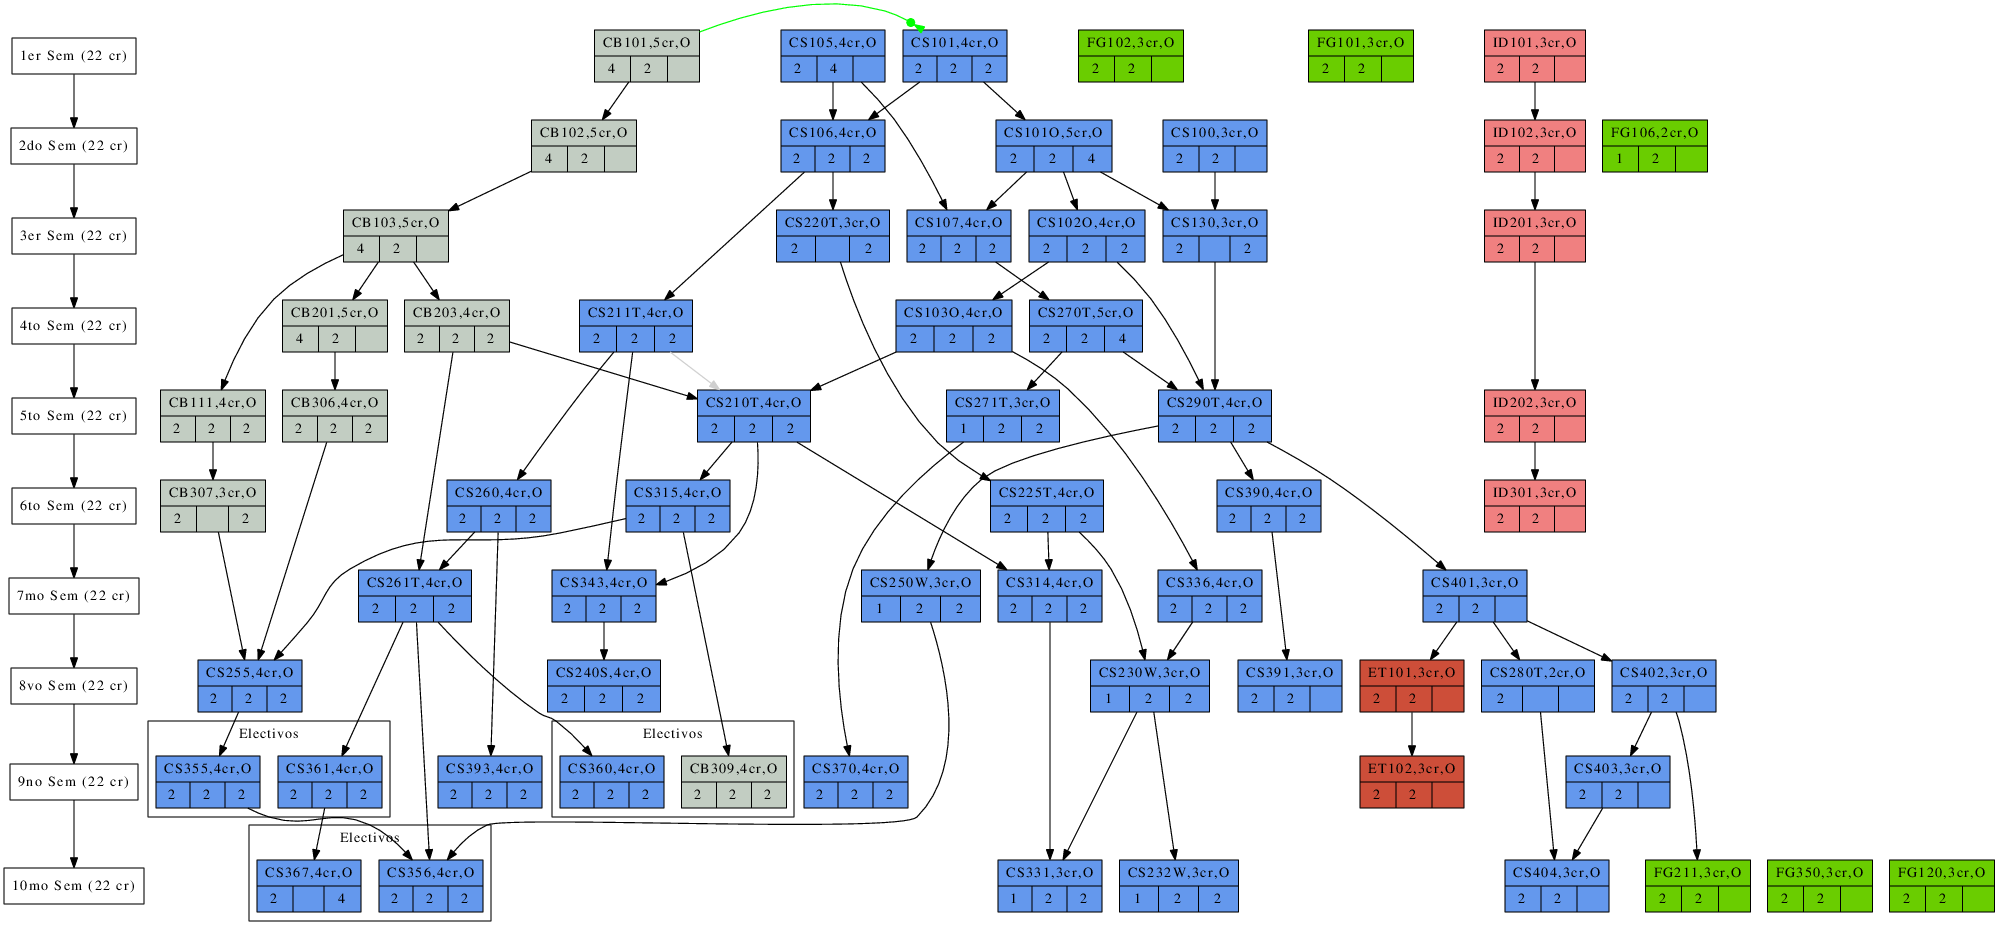
\includegraphics[width=23cm]{/home/ecuadros/Articles/Curricula/Curricula.Master/../Curricula.out/Peru/CS-UTEC/cycle/2017-I/Plan2017/fig/small-graph-curricula.ps}
      \label{fig:malla-curricular}
      \caption{Malla curricular \SchoolFullName}
\end{figure}
\end{landscape}

\section{Distribución de cursos en la carrera}

Esta propuesta puede ser analizada por el número de créditos dedicados a cada área
y por niveles de cursos (Introductorios, Intermedios, Avanzados y Proyectos).
\vspace{0.5cm}
 
\begin{figure}[h!]
      \centering
      \includegraphics[width=10cm]{/home/ecuadros/Articles/Curricula/Curricula.Master/../Curricula.out/Peru/CS-UTEC/cycle/2017-I/Plan2017/fig/pie-credits}
      \label{fig:pie-credits}
      \caption{Distribución de cursos por áreas considerando creditaje.}
\end{figure}


\begin{table}[h!]
\centering
\begin{tabularx}{10.2cm}{|X|c|c|c|c|c|} \hline
  & \colorbox{cornflowerblue}{{\bf AF}}& \colorbox{chartreuse3}{{\bf AE}}& \colorbox{chartreuse3}{{\bf AB}}& \colorbox{tomato3}{{\bf AC}} &  \\ \hline
{\bf Primer Semestre}& 8 & & 7 & 12  & 27 \\ \hline
{\bf Segundo Semestre}& 8 & & 8 & 9  & 25 \\ \hline
{\bf Tercer Semestre}& 9 & & 8 & 5  & 22 \\ \hline
{\bf Cuarto Semestre}& 12 & & 4 & 7  & 23 \\ \hline
{\bf Quinto Semestre}& 15 & & 6 & 2  & 23 \\ \hline
{\bf Sexto Semestre}& 12 & 4 & & 7  & 23 \\ \hline
{\bf Séptimo Semestre}& 4 & 3 & & 4  & 11 \\ \hline
{\bf Octavo Semestre}& 7 & 6 & & 2  & 15 \\ \hline
{\bf Noveno Semestre}& 4 & 11 & & 2.5  & 17.5 \\ \hline
{\bf Décimo Semestre}& 6 & 7 & & 3  & 16 \\ \hline
 {\bf Total}  & 85 & 31 & 33 & 53.5 & 208.5 \\ \hline
 & 40.7\% & 14.8\% & 15.8\% & 25.6\% &  \\ \hline
\end{tabularx}
\caption{Distribución de cursos por áreas}\label{tab:DistributionCreditsByArea}
\end{table}




\begin{figure}[h!]
      \centering
      \includegraphics[width=10cm]{/home/ecuadros/Articles/Curricula/Curricula.Master/../Curricula.out/Peru/CS-UTEC/cycle/2017-I/Plan2017/fig/pie-by-levels}
      \label{fig:pie-niveles}
      \caption{Distribución de créditos por niveles de cursos.}
\end{figure}
 






















\begin{btSect}[apalike]{curricula-main}
\section*{Referencias Bibliográficas}
\btPrintCited
\end{btSect}
\end{btUnit}
  
\chapter{Contenido detallado por curso}\label{chap:syllabi}

\newcounter{conti}

\addcontentsline{toc}{section}{Primer Semestre}
%


\section{CS1D1. Estructuras Discretas I (Obligatorio)}\label{sec:CS1D1}
\begin{itemize}
\item {\bf Semestre}: 1$^{er}$ Sem. {\bf Créditos}: 4
\item {\bf Horas del curso}: {\bf Teoría}: 2 horas; {\bf Práctica}: 4 horas; 
	\begin{htmlonly}
	\item {\bf Sílabo}:
		\begin{rawhtml}
			<a href="syllabi/CS1D1.pdf">Sílabo (PDF)</a>
			<a href="syllabi/CS1D1.pdf"><img alt="Silabus de CS1D1" src="./figs/pdf.jpeg" style="border: 0px solid ; width: 16px; height: 16px;"></a>
		\end{rawhtml}
	\end{htmlonly}
\item {\bf Prerrequisitos}: Ninguno
\end{itemize}



\begin{figure}
\centering
\includegraphics[scale=0.66]{/home/ecuadros/Articles/Curricula/Curricula.Master/../Curricula.out/Peru/CS-UTEC/cycle/2017-I/Plan2017/fig/CS1D1}
\caption{Cursos relacionados con \htmlref{CS1D1}{sec:CS1D1}}
\label{fig:prereq:CS1D1}
\end{figure}




\subsection{Justificación}

Las estructuras discretas proporcionan los fundamentos teóricos necesarios para la computación. Estos fundamentos no sólo son útiles para desarrollar la computación desde un punto de vista teórico como sucede
En el curso de la teoría computacional, pero también es útil para la práctica de la informática; En particular en aplicaciones tales como verificación,
Criptografía, métodos formales, etc.



\subsection{Objetivos Generales}
\begin{enumerate}
\item Aplicar Correctamente conceptos de matemáticas finitas (conjuntos, relaciones, funciones) para representar datos de problemas reales.
\item Modelar situaciones reales descritas en lenguaje natural, usando lógica proposicional y lógica predicada.
\item Determine las propiedades abstractas de las relaciones binarias.
\item Elijir el método de demostración más apropiado para determinar la veracidad de una propuesta y construir argumentos matemáticos correctos.
\item Interpretar soluciones matemáticas a un problema y determinar su fiabilidad, ventajas y desventajas.
\item Expresar el funcionamiento de un circuito electrónico simple usando álgebra booleana.
\end{enumerate}

\subsection{Contribución a los resultados ({\it Outcomes})}
\begin{description}
    \item \ShowOutcome{a}{2}
    \item \ShowOutcome{i}{3}
    \item \ShowOutcome{j}{2}
\end{description}


\subsection{Contribución a las habilidades de Ciencia de la Computación (IEEE)}
\begin{description}
    \item \ShowCompetence{C1}{a}
    \item \ShowCompetence{C20}{i,j}
\end{description}

\subsection{Unidades}

 \subsubsection{Funciones, relaciones y conjuntos\xspace (13 horas) [Habilidades C1,C20]}
\textbf{Referencias Bibliográficas}: \cite{Grimaldi03,Rosen2007}
   \textbf{Tópicos}
\begin{enumerate}
        \item Conjuntos:
\begin{subtopics}
\item Diagramas de Venn
\item Unión, intersección, complemento
\item Producto Cartesiano
\item Potencia de conjuntos
\item Cardinalidad de Conjuntos finitos
\end{subtopics}\xspace
        \item Relaciones:
\begin{subtopics}
\item Reflexividad, simetria, transitividad
\item Relaciones equivalentes, ordenes parciales
\end{subtopics}\xspace
        \item Funciones:
\begin{subtopics}
\item Suryecciones, inyecciones, biyecciones
\item Inversas
\item Composición
\end{subtopics}\xspace
   \end{enumerate}
   \textbf{Objetivos de Aprendizaje}
\begin{enumerate}
	\item Explicar con ejemplos la terminología básica de funciones, relaciones y conjuntos\xspace [Evaluar]
	\item Realizar las operaciones asociadas con conjuntos, funciones y relaciones\xspace [Evaluar]
	\item Relacionar ejemplos prácticos para conjuntos funciones o modelos de relación apropiados e interpretar la asociación de operaciones y terminología en contexto\xspace [Evaluar]
   \end{enumerate}
 

 \subsubsection{Lógica básica\xspace (14 horas) [Habilidades C1,C20]}
\textbf{Referencias Bibliográficas}: \cite{Rosen2007,Grimaldi03}
   \textbf{Tópicos}
\begin{enumerate}
        \item Lógica proposicional.\xspace
        \item Conectores lógicos.\xspace
        \item Tablas de verdad.\xspace
        \item Forma normal (conjuntiva y disyuntiva)\xspace
        \item Validación de fórmula bien formada.\xspace
        \item Reglas de inferencia proposicional (conceptos de modus ponens y modus tollens) \xspace
        \item Logica de predicados:
\begin{subtopics}
\item Cuantificación universal y existencial
\end{subtopics}\xspace
        \item Limitaciones de la lógica proposicional y de predicados (ej. problemas de expresividad)\xspace
   \end{enumerate}
   \textbf{Objetivos de Aprendizaje}
\begin{enumerate}
	\item Convertir declaraciones lógicas desde el lenguaje informal a expresiones de lógica proposicional y de predicados\xspace [Usar ]
	\item Aplicar métodos formales de simbolismo proposicional y lógica de predicados, como el cálculo de la validez de formulas y cálculo de formas normales\xspace [Usar ]
	\item Usar reglas de inferencia para construir demostraciones en lógica proposicional y de predicados\xspace [Usar]
	\item Describir como la lógica simbólica puede ser usada para modelar situaciones o aplicaciones de la vida real, incluidos aquellos planteados en el contexto computacional como análisis de software (ejm. programas correctores ), consulta de base de datos y algoritmos\xspace [Familiarizarse]
	\item Aplicar demostraciones de lógica formal y/o informal, pero rigurosa, razonamiento lógico para problemas reales, como la predicción del comportamiento de software o solución de problemas tales como rompecabezas\xspace [Usar ]
	\item Describir las fortalezas y limitaciones de la lógica proposicional y de predicados\xspace [Usar]
   \end{enumerate}
 

\subsubsection{Técnicas de demostración\xspace (14 horas) [Habilidades C1,C20]}
\textbf{Referencias Bibliográficas}: \cite{Rosen2007, Epp10, Scheinerman12}
\textbf{Tópicos}
\begin{enumerate}
        \item Nociones de implicancia, equivalencia, conversión, inversa, contrapositivo, negación, y contradicción\xspace
        \item Estructura de pruebas matemáticas.\xspace
        \item Demostración directa.\xspace
        \item Refutar por contraejemplo.\xspace
        \item Demostracción por contradicción.\xspace
        \item Inducción sobre números naturales.\xspace
        \item Inducción estructural.\xspace
        \item Inducción leve y fuerte (Ej. Primer y Segundo principio de la inducción)\xspace
        \item Definiciones matemáticas recursivas.\xspace
        \item Conjuntos bien ordenados.\xspace
\end{enumerate}

\textbf{Objetivos de Aprendizaje}
\begin{enumerate}
	\item Identificar la técnica de demostración utilizada en una demostración dada\xspace [Evaluar]
	\item Describir la estructura básica de cada técnica de demostración (demostración directa, demostración por contradicción e inducción) descritas en esta unidad\xspace [Usar ]
	\item Aplicar las técnicas de demostración (demostración directa, demostración por contradicción e inducción) correctamente en la construcción de un argumento solido\xspace [Usar ]
	\item Determine que tipo de demostración es la mejor para un problema dado\xspace [Evaluar]
	\item Explicar el paralelismo entre ideas matemáticas y/o inducción estructural para la recursión y definir estructuras recursivamente\xspace [Familiarizarse ]
	\item Explicar la relación entre inducción fuerte y débil y dar ejemplos del apropiado uso de cada uno\xspace [Evaluar]
	\item Enunciar el principio del buen-orden y su relación con la inducción matemática\xspace [Familiarizarse]
\end{enumerate}


\subsubsection{Lógica Digital y Representación de Datos (19 horas) [Habilidades C1,C20]}
\textbf{Referencias Bibliográficas}: \cite{Rosen2007,Grimaldi03}
   \textbf{Tópicos}
\begin{enumerate}
	\item Órdenes parciales y Conjuntos parcialmente ordenados.   
 	\item Elementos extremos de un conjunto parcialmente ordenado.
	\item Reticulo: Tipos y propiedades.
	\item Álgebras booleanas.
	\item Funciones y expresiones booleanas.
	\item Representación de las funciones booleanas: Disjuntiva normal y forma conjunta.
	\item Puertas Lógicas.
	\item Minimización del Circuito.
   \end{enumerate}

   \textbf{Objetivos de Aprendizaje}
\begin{enumerate}
	\item Explicar la importancia del álgebra booleana como una unificación de la teoría de conjuntos y la lógica proposicional [Evaluar].
	\item Conocer las estructuras algebraicas del retículo y sus tipos [Evaluar].
	\item Explicar la relación entre el retículo y el conjunto de ordenadas y el uso prudente para demostrar que un conjunto es un retículo [Evaluar].
	\item Conocer las propiedades que satisfacen un álgebra booleana [Evaluar].
	\item Demostrar si una terna formada por un conjunto y dos operaciones internas es o no Álgebra booleana [Evaluar].
	\item Encuentra las formas canónicas de una función booleana  [Evaluar].
	\item Representar una función booleana como un circuito booleano usando puertas lógica[Evaluar].
	\item Minimizar una función booleana [Evaluar].
    \end{enumerate}




\newpage%


\section{CS50. Introducción a la Ciencia de la Computación (Obligatorio)}\label{sec:CS111}
\begin{itemize}
\item {\bf Semestre}: 1$^{er}$ Sem. {\bf Créditos}: 4
\item {\bf Horas del curso}: {\bf Teoría}: 3 horas; {\bf Práctica}: 2 horas; 
	\begin{htmlonly}
	\item {\bf Sílabo}:
		\begin{rawhtml}
			<a href="syllabi/CS111.pdf">Sílabo (PDF)</a>
			<a href="syllabi/CS111.pdf"><img alt="Silabus de CS111" src="./figs/pdf.jpeg" style="border: 0px solid ; width: 16px; height: 16px;"></a>
		\end{rawhtml}
	\end{htmlonly}
\item {\bf Prerrequisitos}: Ninguno
\end{itemize}



\begin{figure}
\centering
\includegraphics[scale=0.66]{/home/ecuadros/Articles/Curricula/Curricula.Master/../Curricula.out/Peru/CS-UTEC/cycle/2017-I/Plan2017/fig/CS111}
\caption{Cursos relacionados con \htmlref{CS111}{sec:CS111}}
\label{fig:prereq:CS111}
\end{figure}




\subsection{Justificación}

Este es el primer curso en la secuencia de los cursos introductorios a la Ciencia de la Computación. 
En este curso se pretende cubrir los conceptos señalados por la Computing Curricula IEEE-CS/ACM 2013, bajo el enfoque orientado a objetos.
La programación es uno de los pilares de la Ciencia de la Computación; cualquier profesional del Área, necesitará programar para concretizar sus modelos y propuestas.
Este curso introdución a los participantes en los conceptos fundamentales de este arte. 
Lo tópicos incluyen tipos de datos, estructuras de control, funciones, listas, recursividad y la mecánica de la ejecución, prueba y depuración.


\subsection{Objetivos Generales}
\begin{enumerate}
\item Introducir los conceptos fundamentales de programación durante la construcción de un video juego
\item Desarrollar su capacidad de abstracción, utilizar un lenguaje de programación orientado a objetos.
\end{enumerate}

\subsection{Contribución a los resultados ({\it Outcomes})}
\begin{description}
    \item \ShowOutcome{a}{2}
    \item \ShowOutcome{b}{2}
    \item \ShowOutcome{c}{2}
    \item \ShowOutcome{i}{2}
    \item \ShowOutcome{k}{1}
\end{description}


\subsection{Contribución a las habilidades de Ciencia de la Computación (IEEE)}
\begin{description}
    \item \ShowCompetence{C1}{a} 
    \item \ShowCompetence{C2}{b,c,k} 
    \item \ShowCompetence{C5}{b} 
    \item \ShowCompetence{C4}{i}
\end{description}

\subsection{Unidades}

\subsubsection{Historia\xspace (5 horas) [Habilidades C4]}
\textbf{Referencias Bibliográficas}: \cite{Brookshear11,Guttag13,Zelle10}
    \textbf{Tópicos}
\begin{enumerate}
        \item Pre-historia -- El mundo antes de 1946.\xspace
        \item Historia del hardware, software, redes.\xspace
        \item Pioneros de la Computación.\xspace
        \item Historia de Internet.\xspace
    \end{enumerate}
    
    \textbf{Objetivos de Aprendizaje}
\begin{enumerate}
        \item Identificar importantes tendencias en la historia del campo de la computación\xspace [Familiarizarse]
        \item Identificar las contribuciones de varios pioneros en el campo de la computación\xspace [Familiarizarse]
        \item Discutir el contexto histórico de los paradigmas de diversos lenguajes de programación\xspace [Familiarizarse]
        \item Comparar la vida diaria antes y después de la llegada de los ordenadores personales y el Internet\xspace [Evaluar] 
    \end{enumerate}


\subsubsection{Sistemas de tipos básicos\xspace (2 horas) [Habilidades C1]}
\textbf{Referencias Bibliográficas}: \cite{Guttag13,Zelle10}
    \textbf{Tópicos}
\begin{enumerate}
        \item Tipos como conjunto de valores junto con un conjunto de operaciones.
\begin{subtopics}
\item Tipos primitivos (p.e. numeros, booleanos)
\item Composición de tipos construidos de otros tipos (p.e., registros, uniones, arreglos, listas, funciones, referencias)
\end{subtopics}\xspace
        \item Asociación de tipos de variables, argumentos, resultados y campos.\xspace
		\item Tipo de seguridad y los errores causados por el uso de valores de manera incompatible dadas sus tipos previstos.\xspace
    \end{enumerate}

    \textbf{Objetivos de Aprendizaje}
\begin{enumerate}
		\item Tanto para tipo primitivo y un tipo compuesto, describir de manera informal los valores que tiene dicho tipo\xspace [Familiarizarse]  
		\item Para un lenguaje con sistema de tipos estático, describir las operaciones que están prohibidas de forma estática, como pasar el tipo incorrecto de valor a una función o método\xspace [Familiarizarse]
		\item Describir ejemplos de errores de programa detectadas por un sistema de tipos\xspace [Familiarizarse]
		\item Para múltiples lenguajes de programación, identificar propiedades de un programa con verificación estática y propiedades de un programa con verificación dinámica\xspace [Usar] 
		\item Usar tipos y mensajes de error de tipos para escribir y depurar programas\xspace [Usar] 
		\item Definir y usar piezas de programas (tales como, funciones, clases, métodos) que usan tipos genéricos, incluyendo para colecciones\xspace [Usar] 
    \end{enumerate}


\subsubsection{Conceptos Fundamentales de Programación\xspace (9 horas) [Habilidades C1]}
\textbf{Referencias Bibliográficas}: \cite{Guttag13,Zelle10}
    \textbf{Tópicos}
\begin{enumerate}
        \item Sintaxis y semántica básica de un lenguaje de alto nivel.\xspace
        \item Variables y tipos de datos primitivos (ej., numeros, caracteres, booleanos)\xspace
        \item Expresiones y asignaciones.\xspace
        \item Operaciones básicas I/O incluyendo archivos I/O.\xspace
        \item Estructuras de control condicional e iterativas.\xspace
        \item Paso de funciones y parámetros.\xspace
        \item Concepto de recursividad.\xspace
    \end{enumerate}

    \textbf{Objetivos de Aprendizaje}
\begin{enumerate}
        \item Analiza y explica el comportamiento de programas simples que involucran estructuras fundamentales de programación variables, expresiones, asignaciones, E/S, estructuras de control, funciones, paso de parámetros, y recursividad\xspace [Evaluar] 
        \item Identifica y describe el uso de tipos de datos primitivos\xspace [Familiarizarse]
        \item Escribe programas que usan tipos de datos primitivos\xspace [Usar] 
        \item Modifica y expande programas cortos que usen estructuras de control condicionales e iterativas así como funciones\xspace [Usar] 
        \item Diseña, implementa, prueba, y depura un programa que usa cada una de las siguientes estructuras de datos fundamentales: cálculos básicos, E/S simple, condicional estándar y estructuras iterativas, definición de funciones, y paso de parámetros\xspace [Usar] 
        \item Escribe un programa que usa E/S de archivos para brindar persistencia a través de ejecuciones múltiples\xspace [Usar] 
        \item Escoje estructuras de condición y repetición adecuadas para una tarea de programación dada\xspace [Familiarizarse]
        \item Describe el concepto de recursividad y da ejemplos de su uso\xspace [Evaluar] 
        \item Identifica el caso base y el caso general de un problema basado en recursividad\xspace [Familiarizarse]
    \end{enumerate}


\subsubsection{Análisis Básico\xspace (2 horas) [Habilidades C1,C5]}
\textbf{Referencias Bibliográficas}: \cite{Guttag13,Zelle10}
    \textbf{Tópicos}
\begin{enumerate}
        \item Diferencias entre el mejor, el esperado y el peor caso de un algoritmo.\xspace
        \item Definición formal de la Notación Big O.\xspace
        \item Clases de complejidad como constante, logarítmica, lineal, cuadrática y exponencial.\xspace
        \item Uso de la notación Big O.\xspace
        \item Análisis de algoritmos iterativos y recursivos.\xspace
    \end{enumerate}

    \textbf{Objetivos de Aprendizaje}
\begin{enumerate}
	\item Explique a que se refiere con ``mejor", ``esperado" y ``peor" caso de comportamiento de un algoritmo\xspace [Familiarizarse] 
        \item En el contexto de a algoritmos específicos, identifique las características de data y/o otras condiciones o suposiciones que lleven a diferentes comportamientos\xspace [Familiarizarse] 
        \item Indique la definición formal de Big O\xspace [Familiarizarse] 
        \item Use la notación formal de la Big O para dar límites superiores asintóticos en la complejidad de tiempo y espacio de los algoritmos\xspace [Usar] 
        \item Usar la notación formal Big O para dar límites de casos esperados en el tiempo de complejidad de los algoritmos\xspace [Usar] 
    \end{enumerate}


\subsubsection{Algoritmos y Estructuras de Datos fundamentales\xspace (8 horas) [Habilidades C1,C2,C5]}
\textbf{Referencias Bibliográficas}: \cite{Guttag13,Zelle10}
    \textbf{Tópicos}
\begin{enumerate}
        \item Algoritmos numéricos simples, tales como el cálculo de la media de una lista de números, encontrar el mínimo y máximo.\xspace
        \item Algoritmos de búsqueda secuencial y binaria.\xspace
        \item Algoritmos de ordenamiento de peor caso cuadrático (selección, inserción)\xspace
        \item Algoritmos de ordenamiento con peor caso o caso promedio en O(N lg N) (Quicksort, Heapsort, Mergesort)\xspace
        \item Tablas Hash, incluyendo estratégias para evitar y resolver colisiones.\xspace
        \item Árboles de búsqueda binaria:
\begin{subtopics} 
\item Operaciones comunes en árboles de búsqueda binaria como seleccionar el mínimo, máximo, insertar, eliminar, recorrido en árboles. 
\end{subtopics}\xspace
        \item Grafos y algoritmos en grafos:
\begin{subtopics} 
\item Representación de grafos (ej., lista de adyacencia, matriz de adyacencia) 
\item Recorrido en profundidad y amplitud
\end{subtopics}\xspace
        \item Montículos (Heaps)\xspace
        \item Grafos y algoritmos en grafos:
\begin{subtopics} 
\item Algoritmos de la ruta más corta (algoritmos de Dijkstra y Floyd)
\item Árbol de expansión mínima (algoritmos de Prim y Kruskal) 
\end{subtopics}\xspace
        \item Búsqueda de patrones y algoritmos de cadenas/texto (ej. búsqueda de subcadena, búsqueda de expresiones regulares, algoritmos de subsecuencia común más larga)\xspace
    \end{enumerate}

    \textbf{Objetivos de Aprendizaje}
\begin{enumerate}
        \item Implementar algoritmos numéricos básicos\xspace [Usar] 
        \item Implementar algoritmos de busqueda simple y explicar las diferencias en sus tiempos de complejidad\xspace [Evaluar] 
        \item Ser capaz de implementar algoritmos de ordenamiento comunes cuádraticos y O(N log N)\xspace [Usar] 
        \item Describir la implementación de tablas hash, incluyendo resolución y el evitamiento de colisiones\xspace [Familiarizarse] 
        \item Discutir el tiempo de ejecución y eficiencia de memoria de los principales algoritmos de ordenamiento, busqueda y hashing\xspace [Familiarizarse]
        \item Discutir factores otros que no sean eficiencia computacional que influyan en la elección de algoritmos, tales como tiempo de programación, mantenibilidad, y el uso de patrones específicos de la aplicación en los datos de entrada\xspace [Familiarizarse]
        \item Explicar como el balanceamiento del arbol afecta la eficiencia de varias operaciones de un arbol de búsqueda binaria\xspace [Familiarizarse] 
        \item Resolver problemas usando algoritmos básicos de grafos, incluyendo busqueda por profundidad y busqueda por amplitud\xspace [Usar] 
        \item Demostrar habilidad para evaluar algoritmos, para seleccionar de un rango de posibles opciones, para proveer una  justificación por esa selección,y para implementar el algoritmo en un contexto en específico\xspace [Evaluar] 
        \item Describir la propiedad del heap y el uso de heaps como una implementación de colas de prioridad\xspace [Familiarizarse]
        \item Resolver problemas usando algoritmos de grafos, incluyendo camino más corto de una sola fuente y camino más corto de todos los pares, y como mínimo un algoritmo de arbol de expansion minima\xspace [Usar] 
        \item Trazar y/o implementar un algoritmo de comparación de string\xspace [Usar] 
    \end{enumerate}


\subsubsection{Algoritmos y Diseño\xspace (9 horas) [Habilidades C1,C2,C5]}
\textbf{Referencias Bibliográficas}: \cite{Guttag13,Zelle10}
    \textbf{Tópicos}
\begin{enumerate}
        \item Conceptos y propiedades de los algoritmos
\begin{subtopics}
\item Comparación informal de la eficiencia de los algoritmos (ej., conteo de operaciones)
\end{subtopics}\xspace
        \item Rol de los algoritmos en el proceso de solución de problemas\xspace
        \item Estrategias de solución de problemas
\begin{subtopics}
\item Funciones matemáticas iterativas y recursivas 
\item Recorrido iterativo y recursivo en estructura de datos
\item Estrategias Divide y Conquistar
\end{subtopics}\xspace
        \item Conceptos y principios fundamentales de diseño
\begin{subtopics}
\item Abstracción
\item Descomposición de Program 
\item Encapsulamiento y camuflaje de información 
\item Separación de comportamiento y aplicación
\end{subtopics}\xspace
    \end{enumerate}

    \textbf{Objetivos de Aprendizaje}
\begin{enumerate}
        \item Discute la importancia de los algoritmos en el proceso de solución de un problema\xspace [Familiarizarse]
        \item Discute como un problema puede ser resuelto por múltiples algoritmos, cada uno con propiedades diferentes\xspace [Familiarizarse] 
        \item Crea algoritmos para resolver problemas simples\xspace [Usar] 
        \item Usa un lenguaje de programación para implementar, probar, y depurar algoritmos para resolver problemas simples\xspace [Usar] 
        \item Implementa, prueba, y depura funciones recursivas simples y sus procedimientos\xspace [Usar] 
        \item Determina si una solución iterativa o recursiva es la más apropiada para un problema\xspace [Evaluar] 
        \item Implementa un algoritmo de divide y vencerás para resolver un problema\xspace [Usar] 
        \item Aplica técnicas de descomposición para dividir un programa en partes más pequeñas\xspace [Usar] 
        \item Identifica los componentes de datos y el comportamiento de mútiples tipos de datos abstractos\xspace [Usar] 
        \item Implementa un tipo de dato abstracto coherente, con la menor pérdida de acoplamiento entre componentes y comportamientos\xspace [Usar] 
        \item Identifica las fortalezas y las debilidades relativas entre múltiples diseños e implementaciones de un problema\xspace [Evaluar] 
    \end{enumerate}


\subsubsection{Programación orientada a objetos\xspace (4 horas) [Habilidades C2]}
\textbf{Referencias Bibliográficas}: \cite{Guttag13,Zelle10}
    \textbf{Tópicos}
\begin{enumerate}
        \item Lenguajes orientados a objetos para la encapsulación:
\begin{subtopics} 
\item privacidad y la visibilidad de miembros de la clase 
\item Interfaces revelan único método de firmas 
\item clases base abstractas 
\end{subtopics}\xspace
        \item Definición de las categorías, campos, métodos y constructores.\xspace
        \item Las subclases, herencia y método de alteración temporal.\xspace
        \item Subtipificación:
\begin{subtopics} 
\item Polimorfismo artículo Subtipo; upcasts implícitos en lenguajes con tipos.
\item Noción de reemplazo de comportamiento: los subtipos de actuar como supertipos.
\item Relación entre subtipos y la herencia.
\end{subtopics}\xspace
        \item Lenguajes orientados a objetos para la encapsulación:
\begin{subtopics} 
\item privacidad y la visibilidad de miembros de la clase 
\item Interfaces revelan único método de firmas 
\item clases base abstractas 
\end{subtopics}\xspace
    \end{enumerate}

    \textbf{Objetivos de Aprendizaje}
\begin{enumerate}
        \item Diseñar e implementar una clase\xspace [Usar] 
        \item Usar subclase para diseñar una jerarquía simple de clases que permita al código ser reusable por diferentes subclases\xspace [Familiarizarse] 
        \item Comparar y contrastar (1) el enfoque procedurar/funcional- definiendo una función por cada operación con el cuerdo de la función proporcionando un caso por cada variación de dato - y (2) el enfoque orientado a objetos - definiendo una clase por cada variación de dato con la definición de la clase proporcionando un método por cada operación. Entender ambos enfoques como una definición de variaciones y operaciones de una matriz\xspace [Familiarizarse]
        \item Explicar la relación entre la herencia orientada a objetos (codigo compartido y {\it overriding}) y subtipificación (la idea de un subtipo es ser utilizable en un contexto en el que espera al supertipo)\xspace [Familiarizarse] 
        \item Usar mecanismos de encapsulación orientada a objetos, tal como interfaces y miembros privados\xspace [Familiarizarse]
    \end{enumerate}


\subsubsection{Métodos de Desarrollo\xspace (1 horas) [Habilidades C2]}
\textbf{Referencias Bibliográficas}: \cite{Guttag13,Zelle10}
    \textbf{Tópicos}
\begin{enumerate}
        \item Entornos modernos de programación:
\begin{subtopics}
\item Búsqueda de código.
\item Programación usando libreria de componentes y sus APIs.
\end{subtopics}\xspace
    \end{enumerate}

    \textbf{Objetivos de Aprendizaje}
\begin{enumerate}
        \item Construir y depurar programas que utilizan las bibliotecas estándar disponibles con un lenguaje de programación elegido\xspace [Familiarizarse] 
    \end{enumerate}




\newpage%


\section{CB121. Quimica General (Obligatorio)}\label{sec:CQ121}
\begin{itemize}
\item {\bf Semestre}: 1$^{er}$ Sem. {\bf Créditos}: 3
\item {\bf Horas del curso}: {\bf Teoría}: 3 horas; 
	\begin{htmlonly}
	\item {\bf Sílabo}:
		\begin{rawhtml}
			<a href="syllabi/CQ121.pdf">Sílabo (PDF)</a>
			<a href="syllabi/CQ121.pdf"><img alt="Silabus de CQ121" src="./figs/pdf.jpeg" style="border: 0px solid ; width: 16px; height: 16px;"></a>
		\end{rawhtml}
	\end{htmlonly}
\item {\bf Prerrequisitos}: Ninguno
\end{itemize}



\begin{figure}
\centering
\includegraphics[scale=0.66]{/home/ecuadros/Articles/Curricula/Curricula.Master/../Curricula.out/Peru/CS-UTEC/cycle/2017-I/Plan2017/fig/CQ121}
\caption{Cursos relacionados con \htmlref{CQ121}{sec:CQ121}}
\label{fig:prereq:CQ121}
\end{figure}




\subsection{Justificación}

Este curso es útil en esta carrera para que el alumno aprenda a mostrar un alto grado de dominio de las leyes de la Química General.


\subsection{Objetivos Generales}
\begin{enumerate}
\item Capacitar y presentar al estudiante los principios básicos de la química como ciencia natural abarcando sus tópicos más importantes y su relación con los problemas cotidianos.
\end{enumerate}

\subsection{Contribución a los resultados ({\it Outcomes})}
\begin{description}
\item \ShowOutcome{d}{2}
\item \ShowOutcome{h}{2}
\end{description}


\subsection{Contribución a las habilidades de Ciencia de la Computación (IEEE)}
\begin{description}
    \item \ShowCompetence{C20}{d,h}
\end{description}

\subsection{Unidades}

\subsubsection{QU1. Termodinámica (4 horas) [Habilidades C20]}
\textbf{Referencias Bibliográficas}: \cite{Raymond99,Kennet92}
\textbf{Tópicos}
\begin{enumerate}
      \item Sistemas termodinámicos y su clasificación. Variables termodinámicas y funciones de estado.
      \item Estados de un sistema. Estados de equilibrio. Variables extensivas e intensivas.
      \item Equilibrios térmicos. Principio cero de la termodinámica.
      \item Primer principio de la termodinámica. Capacidad calorífica. Procesos reversibles y trabajo máximo.
      \item Energía interna de los gases ideales. Transformaciones adiabáticas. Termoquímica. Ley de Lavoisier y La Place, Ley de Hess. Ley de Kirchhoff.
      \item Segunda Ley de la termodinámica. Entropía. Eficiencia de un ciclo reversible.
	\item Energía libre. Tercera ley de la termodinámica.
   \end{enumerate}

   \textbf{Objetivos de Aprendizaje}
\begin{enumerate}
      \item Entender y trabajar con los principios de la Termodinámica.
      \item Abstraer de la naturaleza los conceptos de las transformaciones de los gases.
   \end{enumerate}


\subsubsection{QU2. Equilibrio Químico (4 horas) [Habilidades C20]}
\textbf{Referencias Bibliográficas}: \cite{Raymond99,Kennet92}
\textbf{Tópicos}
\begin{enumerate}
      \item Concepto. Constante de equilibrio.
      \item Ley de acción de las masas.
      \item Equilibrios homogéneos. Equilibrios heterogéneos. Equilibrios múltiples.
      \item Factores que afectan el equilibrio químico. Principio de Le Chatelier.
    \end{enumerate}
   \textbf{Objetivos de Aprendizaje}
\begin{enumerate}
      \item Describir, conocer y aplicar los conceptos del equilibrio químico.
      \item Resolver problemas.
   \end{enumerate}


\subsubsection{QU3. Estudios que Contribuyeron al Desarrollo de la Teoría del Átomo (4 horas) [Habilidades C20]}
\textbf{Referencias Bibliográficas}: \cite{Raymond99}
\textbf{Tópicos}
\begin{enumerate}
      \item Propiedades de las ondas.
      \item Radiación electromagnética. Característica. Espectros.
      \item Teoría Cuántica de Max Planck.
      \item Efecto fotoeléctrico.
      \item Relación entre la materia y energía.
      \item Rayos X, Rayos catódicos y rayos canales.
      \item Ejercicios y problemas
\end{enumerate}

   \textbf{Objetivos de Aprendizaje}
\begin{enumerate}
      \item Describir el comportamiento y características de las ondas.
      \item Entender qualitativa y quantitativamente el comportamiento corpuscular de las ondas electromagnéticas.
      \item Resolver problemas.
   \end{enumerate}


\subsubsection{QU4. Teorías del Átomo (6 horas) [Habilidades C20]}
\textbf{Referencias Bibliográficas}: \cite{Babor83,Kennet92}
\textbf{Tópicos}
\begin{enumerate}
      \item Postulados de Dalton. Modelo atómico de Thompson.
      \item Experimento de Rutherford, Modelo atómico de Rutherford. Inconsistencia.
      \item Modelo atómico de Bohr. Espectro de emisión del átomo de hidrógeno.
      \item Teoría atómica moderna. Dualidad de la materia.
      \item Principio de incertidumbre de Heisenberg.
      \item Orbitales atómicos. Ecuación de Schrodinguer.
      \item Descripción mecánico cuántica del átomo de hidrogeno Números cuánticos.
      \item Configuración electrónica. Principio de exclusión de Pauli.
      \item Regla de Hund. Excepciones.
      \item Paramagnetismo y diamagnetismo. Efecto pantalla.
      \item Ejercicios y problemas.
   \end{enumerate}

   \textbf{Objetivos de Aprendizaje}
\begin{enumerate}
      \item Conocer e interpretar los modelos atómicos clásicos.
      \item Entender los fundamentos de la teoría atómica moderna.
      \item Conocer los conceptos básicos de la mecánica cuántica.
      \item Resolver problemas.
   \end{enumerate}


\subsubsection{QU5. Tabla Periódica (4 horas) [Habilidades C20]}
\textbf{Referencias Bibliográficas}: \cite{Kennet92,Mahan92}
\textbf{Tópicos}
\begin{enumerate}
	\item Ley periódica.
	\item Descripción de la tabla periódica. Periodo y grupo. Ubicación de un elemento.
	\item Propiedades periódicas: Radio atómico, radio iónico, energía de ionización, afinidad electrónica. Electronegatividad.
	\item Variación de las propiedades químicas.
	\item Ejercicios y problemas.
   \end{enumerate}

   \textbf{Objetivos de Aprendizaje}
\begin{enumerate}
      \item Entender la estructura de la tabla periódica.
      \item Conocer las propiedades de los elementos.
      \item Resolver problemas.
   \end{enumerate}


\subsubsection{QU6. Enlace Químico (3 horas) [Habilidades C20]}
\textbf{Referencias Bibliográficas}: \cite{Mahan92,Ander83}
   \textbf{Tópicos}
\begin{enumerate}
	\item Teoría de  la valencia. Evolución.
	\item Regla del octeto.
	\item Teoría de Lewis.
	\item Enlace iónico y electrovalente.
	\item Formación del par iónico entre los elementos $s$ y los elementos $p$. Las energías iónicas de las redes cristalinas.
	\item Ciclo de Born Haber.
	\item Enlace covalente. Compartición de pares de electrones.
	\item Carga formal y estructura de Lewis. Concepto de resonancia.
	\item Excepciones a la regla del octeto. Fuerzas en enlace covalente.
	\item Teoría de la repulsión de pares electrónicos del nivel de valencia (RPENV).
	\item Concepto de hibridación. Hibridación sp, sp2, sp3 y otros tipos de hibridación.
	\item Teoría del orbital molecular.
	\item Ejercicios y problemas.
   \end{enumerate}

   \textbf{Objetivos de Aprendizaje}
\begin{enumerate}
      \item Conocer y entender las teorías de valencia y de enlaces químicos.
      \item Conocer y entender la teoría del orbital molecular.
      \item Resolver problemas.
   \end{enumerate}


\subsubsection{QU7. Gases (4 horas) [Habilidades C20]}
\textbf{Referencias Bibliográficas}: \cite{Ander83,Masterton98}
\textbf{Tópicos}
\begin{enumerate}
      \item Definición. Presión de un gas.
      \item Leyes de los gases: de Boyle, Gay-Lussac y Charles. Ecuación de un gas ideal.
      \item Ley de presiones parciales de Dalton.
      \item Teoría cinética de los gases. Distribución de velocidades moleculares. Trayectoria libre media.
      \item Ley de Graham de la difusión y efusión.
      \item Gases reales. Ecuación de Van der Waals.
      \item Ejercicios y problemas.
   \end{enumerate}

   \textbf{Objetivos de Aprendizaje}
\begin{enumerate}
      \item Conocer los conceptos básicos de los gases ideales.
      \item Entender y aplicar la teoría cinética de los gases.
      \item Conocer conceptos de difusión y efusión de gases.
      \item Entender los conceptos de gases reales.
      \item Resolver problemas.
   \end{enumerate}


\subsubsection{QU8. Fuerzas Intermoleculares y Líquidos (3 horas) [Habilidades C20]}
\textbf{Referencias Bibliográficas}: \cite{Masterton98,Babor83}
\textbf{Tópicos}
\begin{enumerate}
      \item Definición. La evaporación y la presión de vapor en el estado de equilibrio.
      \item Medida de la presión de vapor y del calor de vaporización. Punto de ebullición y calor latente de vaporización.
      \item Fuerzas intermoleculares; fuerzas dipolo-dipolo, ion-dipolo, disperso, fuerza y radio de van der Waals. Enlace de hidrógeno.
      \item Viscocidad. Tensión superficial y acción capilar.
      \item Cambios de fase.
      \item Ejercicios y problemas.
    \end{enumerate}

   \textbf{Objetivos de Aprendizaje}
\begin{enumerate}
      \item Conocer conceptos básicos de las fuerzas intermoleculares.
      \item Conocer y aplicar conceptos de vaporización y ebullición.
      \item Conocer y aplicar conceptos de tensión superficial y cambios de fase.
      \item Resolver problemas.
   \end{enumerate}


\subsubsection{QU9. Sólidos (3 horas) [Habilidades C20]}
\textbf{Referencias Bibliográficas}: \cite{Masterton98,Babor83}
\textbf{Tópicos}
\begin{enumerate}
      \item Definición. Empaquetación de esferas. Eficiencia de empaquetamiento. Empaquetamiento compacto.
      \item Empleo de los Rayos X en el estudio de la estructura de los cristales.
      \item Clases de estructuras cristalinas: cristales iónicos. Covalentes, moleculares, metálicos. Enlace metálico Cristales amorfos.
      \item Cambios de fase. Equilibrio líquido-vapor. Calor de vaporización y punto de ebullición.
      \item Equilibrio líquido-sólido. Equilibrio sólido-vapor. Diagrama de fase  del agua y del dióxido de carbono.
      \item Ejercicios y problemas.
    \end{enumerate}

   \textbf{Objetivos de Aprendizaje}
\begin{enumerate}
      \item Conocer conceptos básicos de las estructuras cristalinas de sólidos.
      \item Conocer y aplicar conceptos de cambios de fase y de equilibrio.
      \item Resolver problemas.
   \end{enumerate}


\subsubsection{QU10. Disoluciones (3 horas) [Habilidades C20]}
\textbf{Referencias Bibliográficas}: \cite{Masterton98,Babor83}
\textbf{Tópicos}
\begin{enumerate}
      \item Definición. Visión molecular del proceso de disolución.
      \item Disoluciones de líquidos en líquidos. Disoluciones de sólidos en líquidos.
      \item Unidades de concentración: porcentaje en masa, fracción molar, molaridad, molalidad Normalidad.
      \item Efecto de la temperatura en la solubilidad, la solubilidad de los sólidos y la temperatura, cristalización fraccionada.
      \item La solubilidad de los gases y la temperatura. Efecto  de la presión en la solubilidad de los gases.
      \item Propiedades coligativas de las soluciones. Dispersiones coloidales.
      \item Ejercicios y problemas.
    \end{enumerate}

   \textbf{Objetivos de Aprendizaje}
\begin{enumerate}
      \item Conocer conceptos básicos de las disoluciones moleculares.
      \item Conocer y aplicar conceptos de concentración y solubilidad.
      \item Resolver problemas.
   \end{enumerate}


\subsubsection{QU11. Estequiometría (3 horas) [Habilidades C20]}
\textbf{Referencias Bibliográficas}: \cite{Masterton98,Babor83}
\textbf{Tópicos}
\begin{enumerate}
      \item Reacción química. Expresiones de las reacciones químicas en forma de ecuaciones. Características de una ecuación química.
      \item Tipos de reacciones químicas: Precipitación, ácido-base, óxido-reducción. Cantidad de reactivos y productos.
      \item Relaciones estequiométricas: moles, masa y volumen.
      \item Leyes ponderales y volumétricas.
      \item Reactivo limitante. Rendimiento de las reacciones.
      \item Ejercicios y problemas.
    \end{enumerate}

   \textbf{Objetivos de Aprendizaje}
\begin{enumerate}
      \item Conocer conceptos básicos de las reacciones químicas.
      \item Conocer y aplicar las leyes ponderales y volumétricas.
      \item Resolver problemas.
   \end{enumerate}




\newpage%


\section{FG101A. Laboratorio de Comunicación I (Obligatorio)}\label{sec:GH1005}
\begin{itemize}
\item {\bf Semestre}: 1$^{er}$ Sem. {\bf Créditos}: 3
\item {\bf Horas del curso}: {\bf Teoría}: 2 horas; {\bf Práctica}: 2 horas; 
	\begin{htmlonly}
	\item {\bf Sílabo}:
		\begin{rawhtml}
			<a href="syllabi/GH1005.pdf">Sílabo (PDF)</a>
			<a href="syllabi/GH1005.pdf"><img alt="Silabus de GH1005" src="./figs/pdf.jpeg" style="border: 0px solid ; width: 16px; height: 16px;"></a>
		\end{rawhtml}
	\end{htmlonly}
\item {\bf Prerrequisitos}: Ninguno
\end{itemize}



\begin{figure}
\centering
\includegraphics[scale=0.66]{/home/ecuadros/Articles/Curricula/Curricula.Master/../Curricula.out/Peru/CS-UTEC/cycle/2017-I/Plan2017/fig/GH1005}
\caption{Cursos relacionados con \htmlref{GH1005}{sec:GH1005}}
\label{fig:prereq:GH1005}
\end{figure}




\subsection{Justificación}

A través de este curso, el alumno mejorará y fortalecerá sus capacidades para comunicarse tanto a nivel oral como escrito en un contexto académico. Para ello, el alumno se ejercitará en la composición de textos, tomando en cuenta las exigencias propias de un lenguaje formal académico: características de la redacción académica (reglas de puntuación, ortografía, competencia léxico gramatical, normativa) y empleo correcto de la información. A su vez, el curso promueve una lectura comprensiva que no se limita al nivel descriptivo, sino que abarca también lo conceptual y metafórico, pues solo de ese modo el estudiante desarrollará su capacidad crítica y analítica. El estudiante afrontará lecturas académicas y de divulgación científica que le permitirán distinguir los objetivos planteados en los distintos tipos de textos, y reconocer al texto oral y escrito como una unidad coherente y cohesionada en cuanto a forma y contenido. Alcanzados estos objetivos, el estudiante comprenderá que las habilidades comunicativas orales y escritas son competencias centrales de su vida universitaria y, posteriormente, de su vida profesional. 


\subsection{Objetivos Generales}
\begin{enumerate}
\item Con este curso el estudiante desarrolla y fortalece sus habilidades comunicativas orales y escritas en el marco de un contexto académico. Además, comprende conceptual y metafóricamente textos expositivos, e identifica los objetivos, jerarquía de las ideas y estructura de dichos textos. Al finalizar el curso, el estudiante es capaz de producir textos expositivos descriptivos e informativos. Así mismo, desarrolla su capacidad de apertura y tolerancia hacia la diversidad de puntos de vista gracias al continuo trabajo grupal, autoevaluaciones y evaluaciones de pares que enfrentará a lo largo del ciclo en el curso. 
\end{enumerate}

\subsection{Contribución a los resultados ({\it Outcomes})}
\begin{description}
     \item \ShowOutcome{e}{2}
     \item \ShowOutcome{f}{2}
     \item \ShowOutcome{i}{2}
     \item \ShowOutcome{n}{2}
\end{description}


\subsection{Contribución a las habilidades de Ciencia de la Computación (IEEE)}
\begin{description}
    \item \ShowCompetence{C17}{f,h,n}
    \item \ShowCompetence{C20}{f,n}
    \item \ShowCompetence{C24}{f,h}
\end{description}

\subsection{Unidades}

\subsubsection{Laboratorio de Comunicación I (12 horas) [Habilidades 4]}
\textbf{Referencias Bibliográficas}: \cite{Cassany93}
   \textbf{Tópicos}
\begin{enumerate}
      \item Características de Escritura Académica.
      \item Estrategias de Lectura.
      \item Estructura del texto.
      \item Estructura de párrafos.
      \item Características del párrafo.
      \item Texto argumentativo Vs. Texto expositivo.
      \item Proceso de Redacción.
      \item Citas:función y tipos -Bibiliografía.
      \item Aproximación a características de la exposición oral.
      \item Conferencia :caracterpisticas exposición formal.
      \item Redacción de texto completo con citas.  
   \end{enumerate}
   \textbf{Objetivos de Aprendizaje}
\begin{enumerate}
      \item Auto-evaluación: el estudiante es capaz de reconocer sus propias fortalezas y deficiencias al formular críticas constructivas sobre su propio trabajo.
   \end{enumerate}




\newpage%


\section{FG101A. Laboratorio de Comunicación I (Obligatorio)}\label{sec:GH1005}
\begin{itemize}
\item {\bf Semestre}: 1$^{er}$ Sem. {\bf Créditos}: 3
\item {\bf Horas del curso}: {\bf Teoría}: 2 horas; {\bf Práctica}: 2 horas; 
	\begin{htmlonly}
	\item {\bf Sílabo}:
		\begin{rawhtml}
			<a href="syllabi/GH1005.pdf">Sílabo (PDF)</a>
			<a href="syllabi/GH1005.pdf"><img alt="Silabus de GH1005" src="./figs/pdf.jpeg" style="border: 0px solid ; width: 16px; height: 16px;"></a>
		\end{rawhtml}
	\end{htmlonly}
\item {\bf Prerrequisitos}: Ninguno
\end{itemize}



\begin{figure}
\centering
\includegraphics[scale=0.66]{/home/ecuadros/Articles/Curricula/Curricula.Master/../Curricula.out/Peru/CS-UTEC/cycle/2017-I/Plan2017/fig/GH1005}
\caption{Cursos relacionados con \htmlref{GH1005}{sec:GH1005}}
\label{fig:prereq:GH1005}
\end{figure}




\subsection{Justificación}

A través de este curso, el alumno mejorará y fortalecerá sus capacidades para comunicarse tanto a nivel oral como escrito en un contexto académico. Para ello, el alumno se ejercitará en la composición de textos, tomando en cuenta las exigencias propias de un lenguaje formal académico: características de la redacción académica (reglas de puntuación, ortografía, competencia léxico gramatical, normativa) y empleo correcto de la información. A su vez, el curso promueve una lectura comprensiva que no se limita al nivel descriptivo, sino que abarca también lo conceptual y metafórico, pues solo de ese modo el estudiante desarrollará su capacidad crítica y analítica. El estudiante afrontará lecturas académicas y de divulgación científica que le permitirán distinguir los objetivos planteados en los distintos tipos de textos, y reconocer al texto oral y escrito como una unidad coherente y cohesionada en cuanto a forma y contenido. Alcanzados estos objetivos, el estudiante comprenderá que las habilidades comunicativas orales y escritas son competencias centrales de su vida universitaria y, posteriormente, de su vida profesional. 


\subsection{Objetivos Generales}
\begin{enumerate}
\item Con este curso el estudiante desarrolla y fortalece sus habilidades comunicativas orales y escritas en el marco de un contexto académico. Además, comprende conceptual y metafóricamente textos expositivos, e identifica los objetivos, jerarquía de las ideas y estructura de dichos textos. Al finalizar el curso, el estudiante es capaz de producir textos expositivos descriptivos e informativos. Así mismo, desarrolla su capacidad de apertura y tolerancia hacia la diversidad de puntos de vista gracias al continuo trabajo grupal, autoevaluaciones y evaluaciones de pares que enfrentará a lo largo del ciclo en el curso. 
\end{enumerate}

\subsection{Contribución a los resultados ({\it Outcomes})}
\begin{description}
     \item \ShowOutcome{e}{2}
     \item \ShowOutcome{f}{2}
     \item \ShowOutcome{i}{2}
     \item \ShowOutcome{n}{2}
\end{description}


\subsection{Contribución a las habilidades de Ciencia de la Computación (IEEE)}
\begin{description}
    \item \ShowCompetence{C17}{f,h,n}
    \item \ShowCompetence{C20}{f,n}
    \item \ShowCompetence{C24}{f,h}
\end{description}

\subsection{Unidades}

\subsubsection{Laboratorio de Comunicación I (12 horas) [Habilidades 4]}
\textbf{Referencias Bibliográficas}: \cite{Cassany93}
   \textbf{Tópicos}
\begin{enumerate}
      \item Características de Escritura Académica.
      \item Estrategias de Lectura.
      \item Estructura del texto.
      \item Estructura de párrafos.
      \item Características del párrafo.
      \item Texto argumentativo Vs. Texto expositivo.
      \item Proceso de Redacción.
      \item Citas:función y tipos -Bibiliografía.
      \item Aproximación a características de la exposición oral.
      \item Conferencia :caracterpisticas exposición formal.
      \item Redacción de texto completo con citas.  
   \end{enumerate}
   \textbf{Objetivos de Aprendizaje}
\begin{enumerate}
      \item Auto-evaluación: el estudiante es capaz de reconocer sus propias fortalezas y deficiencias al formular críticas constructivas sobre su propio trabajo.
   \end{enumerate}




\newpage%


\section{FG101D. Desafíos Globales (Obligatorio)}\label{sec:FG101D}
\begin{itemize}
\item {\bf Semestre}: 1$^{er}$ Sem. {\bf Créditos}: 3
\item {\bf Horas del curso}: {\bf Teoría}: 2 horas; {\bf Práctica}: 2 horas; 
	\begin{htmlonly}
	\item {\bf Sílabo}:
		\begin{rawhtml}
			<a href="syllabi/FG101D.pdf">Sílabo (PDF)</a>
			<a href="syllabi/FG101D.pdf"><img alt="Silabus de FG101D" src="./figs/pdf.jpeg" style="border: 0px solid ; width: 16px; height: 16px;"></a>
		\end{rawhtml}
	\end{htmlonly}
\item {\bf Prerrequisitos}: Ninguno
\end{itemize}



\begin{figure}
\centering
\includegraphics[scale=0.66]{/home/ecuadros/Articles/Curricula/Curricula.Master/../Curricula.out/Peru/CS-UTEC/cycle/2017-I/Plan2017/fig/FG101D}
\caption{Cursos relacionados con \htmlref{FG101D}{sec:FG101D}}
\label{fig:prereq:FG101D}
\end{figure}




\subsection{Justificación}

Durante las sesiones plenarias, se realizarán clases magistrales relacionadas a la metodología de Design Thinking así como su uso e importancia en los procesos de creación . Así mismo, durante estas sesiones tendremos ponencias sobre emprendimientos y startups relacionados a la ingeniería o tecnología.
Durante las sesiones de laboratorio, los alumnos forman equipos que mantienen durante el ciclo. Con la guía del profesor y a través de la metodología del Design Thinking desarrollada en las plenarias, los alumnos deberán plantear soluciones innovadoras a problemas reales inspirados en los Global Challenges de las Naciones Unidas.
Los alumnos contarán con una Bitácora Digital que será revisada constantemente por los docentes a cargo. En ella se encontrarán los avances, procesos y referentes del proyecto grupal. El curso culmina con las presentaciones de las propuestas planteadas por los grupos.


\subsection{Objetivos Generales}
\begin{enumerate}
\item Capacidad de diseñar y llevar a cabo experimentos 
\item Capacidad de analizar información
\item Capacidad para diseñar un sistema, un componente o un proceso para satisfacer las necesidades deseadas dentro de restricciones realistas (Nivel 1)
\item Capacidad de trabajo en equipo
\item Capacidad de liderar un equipo
\item Capacidad de comunicación oral (Nivel 1)
\item Capacidad de comunicación escrita (Nivel 1)
\item Comprende el impacto de las soluciones de la ingeniería en un contexto global, económico, ambiental y de la sociedad.

\end{enumerate}

\subsection{Contribución a los resultados ({\it Outcomes})}
\begin{description}
    \item \ShowOutcome{n}{2}
    \item \ShowOutcome{ñ}{2}
\end{description}


\subsection{Contribución a las habilidades de Ciencia de la Computación (IEEE)}
\begin{description}
    \item \ShowCompetence{C20}{n,ñ}
\end{description}

\subsection{Unidades}

\subsubsection{Desafíos Globales (12 horas) [Habilidades 4]}
\textbf{Referencias Bibliográficas}: \cite{Curedale12,Upton15}
   \textbf{Tópicos}
\begin{enumerate}
      \item Pasos de DT.
      \item Técnica y usos del Brainstorm.
      \item Conocimiento del usuario, empatía y uso de arquetipos.
      \item Tipos de Investigación, diferencias y usos.
      \item Estrategias de recolección de Insights.
      \item Métodos de Ideación.
      \item Introducción al Prototipado.
      \item Introducción a la Experiencia de Usuario.
      \item Estrategias de Testeo e Iteración
      \item Usos del Storytelling
   \end{enumerate}
   \textbf{Objetivos de Aprendizaje}
\begin{enumerate}
      \item Flexibilidad y Adaptabilidad: Los alumnos aprenden a trabajar en equipo, en un ambiente flexible, variable y de constantes retos.
   \end{enumerate}




\newpage%


\section{EG1003. Matemática I (Obligatorio)}\label{sec:EG1003}
\begin{itemize}
\item {\bf Semestre}: 1$^{er}$ Sem. {\bf Créditos}: 4
\item {\bf Horas del curso}: {\bf Teoría}: 4 horas; 
	\begin{htmlonly}
	\item {\bf Sílabo}:
		\begin{rawhtml}
			<a href="syllabi/EG1003.pdf">Sílabo (PDF)</a>
			<a href="syllabi/EG1003.pdf"><img alt="Silabus de EG1003" src="./figs/pdf.jpeg" style="border: 0px solid ; width: 16px; height: 16px;"></a>
		\end{rawhtml}
	\end{htmlonly}
\item {\bf Prerrequisitos}: Ninguno
\end{itemize}



\begin{figure}
\centering
\includegraphics[scale=0.66]{/home/ecuadros/Articles/Curricula/Curricula.Master/../Curricula.out/Peru/CS-UTEC/cycle/2017-I/Plan2017/fig/EG1003}
\caption{Cursos relacionados con \htmlref{EG1003}{sec:EG1003}}
\label{fig:prereq:EG1003}
\end{figure}




\subsection{Justificación}

El curso tiene como objetivo desarrollar en los estudiantes las habilidades para manejar modelos en ciencia e ingeniería relacionados con habilidades de cálculo diferencial simple. En el curso se estudian y aplican conceptos relacionados con el cálculo de Límites, derivados e integrales de funciones reales y vectoriales de variables reales únicas que se utilizarán como base y
apoyo al estudio de nuevos contenidos y materias. También busca lograr capacidades de razonamiento y aplicabilidad para interactuar con problemas del mundo real proporcionando una base matemática para actividades de desarrollo.


\subsection{Objetivos Generales}
\begin{enumerate}
\item Aplicar los conceptos de números complejos y funciones para resolver problemas relacionados con la ciencia.
\item Aplicar conceptos matemáticos y técnicas de cálculo diferencial de una variable para resolver situaciones problemáticas de la ciencia
\item Calcular las expresiones matemáticas de las integrales indefinidas con exactitud, orden y claridad en el tratamiento de los datos.

\end{enumerate}

\subsection{Contribución a los resultados ({\it Outcomes})}
\begin{description}
    \item \ShowOutcome{a}{3}
    \item \ShowOutcome{j}{3}
\end{description}


\subsection{Contribución a las habilidades de Ciencia de la Computación (IEEE)}
\begin{description}
    \item \ShowCompetence{C1}{a}
    \item \ShowCompetence{C20}{j}
    \item \ShowCompetence{C24}{j}
\end{description}

\subsection{Unidades}

\subsubsection{Números complejos (20 horas) [Habilidades C1]}
\textbf{Referencias Bibliográficas}: \cite{Stewart,RonLarson}

   \textbf{Tópicos}
\begin{enumerate}
    \item . 
    \item . 
   \end{enumerate}

   \textbf{Objetivos de Aprendizaje}
\begin{enumerate}
      \item . 
      \item . 
      \end{enumerate}


\subsubsection{Funciones de una sola variable (10 horas) [Habilidades C20]}
\textbf{Referencias Bibliográficas}: \cite{Stewart,RonLarson}

  
  \textbf{Tópicos}
\begin{enumerate}
    \item . 
    \item . 
    \item . 
    \item . 
    \item . 
    \item . 
   \end{enumerate}

   \textbf{Objetivos de Aprendizaje}
\begin{enumerate}
      \item . 
      \item . 
      \item . 
      \item . 
      \item . 
      \item . 
    \end{enumerate}


\subsubsection{Límites y derivadas (20 horas) [Habilidades C1]}
\textbf{Referencias Bibliográficas}: \cite{Stewart,RonLarson}

   \textbf{Tópicos}
\begin{enumerate}
      \item . 
      \item . 
      \item . 
      \item . 
      \item . 
   \end{enumerate}

   \textbf{Objetivos de Aprendizaje}
\begin{enumerate}
      \item . 
      \item . 
      \item . 
      \item . 
      \item . 
      \item . 
      \item . 
      \item . 
      \item . 
      \item . 
      \item . 
        \end{enumerate}


\subsubsection{Integrales (22 horas) [Habilidades C20]}
\textbf{Referencias Bibliográficas}: \cite{Stewart,RonLarson}

   \textbf{Tópicos}
\begin{enumerate}
    \item . 
    \item . 
    \item . 
    \item . 

   \end{enumerate}

   \textbf{Objetivos de Aprendizaje}
\begin{enumerate}
      \item . 
      \item . 
      \item . 
      \item . 
      \item . 
      \item . 
      \item . 
      \item . 
      \item . 
      \item . 
      \item . 
    \end{enumerate}




\newpage%


\section{ID101. Inglés I (Obligatorio)}\label{sec:ID101}
\begin{itemize}
\item {\bf Semestre}: 1$^{er}$ Sem. {\bf Créditos}: 3
\item {\bf Horas del curso}: {\bf Práctica}: 10 horas; 
	\begin{htmlonly}
	\item {\bf Sílabo}:
		\begin{rawhtml}
			<a href="syllabi/ID101.pdf">Sílabo (PDF)</a>
			<a href="syllabi/ID101.pdf"><img alt="Silabus de ID101" src="./figs/pdf.jpeg" style="border: 0px solid ; width: 16px; height: 16px;"></a>
		\end{rawhtml}
	\end{htmlonly}
\item {\bf Prerrequisitos}: Ninguno
\end{itemize}



\begin{figure}
\centering
\includegraphics[scale=0.66]{/home/ecuadros/Articles/Curricula/Curricula.Master/../Curricula.out/Peru/CS-UTEC/cycle/2017-I/Plan2017/fig/ID101}
\caption{Cursos relacionados con \htmlref{ID101}{sec:ID101}}
\label{fig:prereq:ID101}
\end{figure}




\subsection{Justificación}

Parte fundamental de la formación integral de un profesional es la habilidad de comunicarse en un idioma extranjero además del propio idioma nativo. No solamente amplí­a su horizonte cultural sino que permite una visión más humana y comprensiva de la vida de las personas. En el caso de los idiomas extranjeros, indudablemente el Inglés es el más prátcico porque es hablado alrededor de todo el mundo. No hay paí­s alguno donde éste no sea hablado. En las carreras relacionadas con los servicios al turista el Inglés es tal vez la herramienta práctica más importante que el alumno debe dominar desde el primer momento, como parte de su formación integral.


\subsection{Objetivos Generales}
\begin{enumerate}
\item Conocer el idioma Inglés y su estructura gramatical.
\item Identificar situaciones y emplear diálogos relacionados a ellas.
\end{enumerate}

\subsection{Contribución a los resultados ({\it Outcomes})}
\begin{description}
\item \ShowOutcome{f}{2}
\end{description}


\subsection{Contribución a las habilidades de Ciencia de la Computación (IEEE)}
\begin{description}
    \item \ShowCompetence{C25}{f}
\end{description}

\subsection{Unidades}

\subsubsection{Hello everybody (0 horas) [Habilidades C25]}
\textbf{Referencias Bibliográficas}: \cite{Soars022S,Cambridge06,MacGrew99}
   \textbf{Tópicos}
\begin{enumerate}
      \item Verbo To Be.
      \item Oraciones Afirmativas, Negativas y Preguntas.
      \item Expresiones Numéricas.
      \item Objetos y Paí­ses.
      \item Expresiones para saludar y hacer presentaciones.
   \end{enumerate}

   \textbf{Objetivos de Aprendizaje}
\begin{enumerate}
      \item Al terminar la primera unidad, cada uno de los alumnos, comprendiendo la gramática del tiempo presente es capaz de expresar una mayor cantidad de expresiones de tiempo y además usar oraciones con el verbo To Be para expresar situación y estado. 
      \item Que el alumno sea capaz de analizar y expresar ideas acerca de fechas y números en orden. 
   \end{enumerate}


\subsubsection{Meeting people (0 horas) [Habilidades C25]}
\textbf{Referencias Bibliográficas}: \cite{Soars022S,Cambridge06,MacGrew99}
   \textbf{Tópicos}
\begin{enumerate}
      \item Adjetivos Posesivos.
      \item Expresiones para averiguar precios.
      \item Expresiones de Posesión.
      \item Vocabulario de Familia, Comidas y Bebidas.
      \item Pedidos formales.
      \item Cartas informales.
   \end{enumerate}

   \textbf{Objetivos de Aprendizaje}
\begin{enumerate}
      \item Al terminar la segunda unidad, los alumnos habiendo identificado la forma de expresar pedidos y hacer ofrecimientos en restaurantes los utilizan en situaciones varias. Explica y aplica vocabulario de comidas y bebidas.  
   \end{enumerate}



\subsubsection{The world of work (0 horas) [Habilidades C25]}
\textbf{Referencias Bibliográficas}: \cite{Soars022S,Cambridge06,MacGrew99}
   \textbf{Tópicos}
\begin{enumerate}
      \item Tiempo Presente Simple. Auxiliares.
      \item Oraciones Afirmativas, Negativas y Preguntas.
      \item Verbos comunes y Ocupaciones.
      \item Indicaciones para expresar la hora.
   \end{enumerate}

   \textbf{Objetivos de Aprendizaje}
\begin{enumerate}
      \item Al terminar la tercera unidad, los alumnos habiendo reconocido las caracterí­sticas del presente simple, lo utiliza para hacer descripciones de diversos tipos. Describen personas y lugares y dan indicaciones de dirección. Expresa la hora. 
   \end{enumerate}



\subsubsection{Take it easy (0 horas) [Habilidades C25]}
\textbf{Referencias Bibliográficas}: \cite{Soars022S,Cambridge06,MacGrew99}
   \textbf{Tópicos}
\begin{enumerate}
      \item Presente Simple 2.
      \item Oraciones Afirmativas, Negativas y Preguntas.
      \item Uso de Verbos de entretenimiento.
      \item Tiempo Libre.
      \item Las estaciones del año.
      \item Expresiones de actividades sociales.
   \end{enumerate}

   \textbf{Objetivos de Aprendizaje}
\begin{enumerate}
      \item Al terminar la cuarta unidad, los alumnos habiendo identificado la idea de expresar ideas de acciones de tiempo libre en Presente Simple y Continuo. Expresan ideas de estaciones y actividades relacionadas.
   \end{enumerate}



\subsubsection{Where do you live ? (0 horas) [Habilidades C25]}
\textbf{Referencias Bibliográficas}: \cite{Soars022S,Cambridge06,MacGrew99}
   \textbf{Tópicos}
\begin{enumerate}
      \item Uso There is/There are.
      \item Oraciones con Preposiciones.
      \item Expresiones de Cantidad.
      \item Vocabulario de aviones y lugares.
      \item Expresiones de indicaciones de dirección.
   \end{enumerate}

   \textbf{Objetivos de Aprendizaje}
\begin{enumerate}
      \item Al finalizar la quinta unidad, los alumnos, a partir de la comprensión del tiempo presente continuo, elaborararán oraciones utilizando ideas de ubicación y de lugar. Asimilarán además la necesidad de expresar objetos de uso común. Adquirirán vocabulario para describir las partes de una casa usan expresiones para pedir indicaciones de dirección.
   \end{enumerate}


\subsubsection{Can you speak English? (0 horas) [Habilidades C25]}
\textbf{Referencias Bibliográficas}: \cite{Soars022S,Cambridge06,MacGrew99}
   \textbf{Tópicos}
\begin{enumerate}
      \item Can/cant.
      \item Pasado del verbo To Be. Uso de Could.
      \item Vocabulario de Paí­ses e idiomas.
      \item Expresiones para el uso del teléfono.
      \item Redacción de cartas formales.
      \item Lecturas.
   \end{enumerate}

   \textbf{Objetivos de Aprendizaje}
\begin{enumerate}
      \item Al finalizar la sexta unidad, los alumnos habiendo conocido los fundamentos del uso de auxiliares de modo, crearan oraciones aplicadas al contexto adecuado. Enfatizan la diferencia entre idiomas y nacionalidades. Describen sentimientos. Utilizan expresiones en el teléfono.
   \end{enumerate}


\subsubsection{Then and now (0 horas) [Habilidades C25]}
\textbf{Referencias Bibliográficas}: \cite{Soars022S,Cambridge06,MacGrew99}
   \textbf{Tópicos}
\begin{enumerate}
      \item Pasado Simple.
      \item Expresiones de tiempo pasado.
      \item Vocabulario verbos regulares e irregulares.
      \item Expresiones para describir el clima. 
      \item Redacción de párrafos descriptivos.
      \item Ocasiones Especiales.
   \end{enumerate}

   \textbf{Objetivos de Aprendizaje}
\begin{enumerate}
      \item Al finalizar la sétima unidad, los alumnos habiendo conocido los fundamentos de la estructuración del Pasado Simple experimentan la necesidad de poder expresar este tipo de tiempo en acciones. Realizarán prácticas en contextos adecuados. Enfatizan la diferencia entre verbos irregulares y regulares. Describen acciones con verbos varios. Utilizan expresiones para describir el clima.
   \end{enumerate}




\addcontentsline{toc}{section}{Segundo Semestre}
\newpage%


\section{CS1D2. Estructuras Discretas II (Obligatorio)}\label{sec:CS1D2}
\begin{itemize}
\item {\bf Semestre}: 2$^{do}$ Sem. {\bf Créditos}: 4
\item {\bf Horas del curso}: {\bf Teoría}: 2 horas; {\bf Práctica}: 4 horas; 
	\begin{htmlonly}
	\item {\bf Sílabo}:
		\begin{rawhtml}
			<a href="syllabi/CS1D2.pdf">Sílabo (PDF)</a>
			<a href="syllabi/CS1D2.pdf"><img alt="Silabus de CS1D2" src="./figs/pdf.jpeg" style="border: 0px solid ; width: 16px; height: 16px;"></a>
		\end{rawhtml}
	\end{htmlonly}
\item {\bf Prerrequisitos}: 
	\begin{itemize}
		\item \htmlref{CS1D1. Estructuras Discretas I}{sec:CS1D1}~(1$^{er}$ Sem-Pág.~\pageref{sec:CS1D1})
	\end{itemize}
\end{itemize}



\begin{figure}
\centering
\includegraphics[scale=0.66]{/home/ecuadros/Articles/Curricula/Curricula.Master/../Curricula.out/Peru/CS-UTEC/cycle/2017-I/Plan2017/fig/CS1D2}
\caption{Cursos relacionados con \htmlref{CS1D2}{sec:CS1D2}}
\label{fig:prereq:CS1D2}
\end{figure}




\subsection{Justificación}

Para entender las técnicas computacionales avanzadas, los estudiantes deberán tener un fuerte conocimiento de las
diversas estructuras discretas, estructuras que serán implementadas y usadas en laboratorio en el lenguaje de programación.


\subsection{Objetivos Generales}
\begin{enumerate}
\item Que el alumno sea capaz de modelar problemas de ciencia de la computación usando grafos y árboles relacionados con estructuras de datos
\item Que el alumno aplicar eficientemente estrategias de recorrido para poder buscar datos de una manera óptima
\end{enumerate}

\subsection{Contribución a los resultados ({\it Outcomes})}
\begin{description}
    \item \ShowOutcome{a}{1}
    \item \ShowOutcome{i}{1}	
    \item \ShowOutcome{j}{1}
\end{description}


\subsection{Contribución a las habilidades de Ciencia de la Computación (IEEE)}
\begin{description}
    \item \ShowCompetence{C1}{a}
    \item \ShowCompetence{C20}{i}
\end{description}

\subsection{Unidades}

\subsubsection{Fundamentos de conteo\xspace (25 horas) [Habilidades C1]}
\textbf{Referencias Bibliográficas}: \cite{Grimaldi97} 
    \textbf{Tópicos}
\begin{enumerate}
        \item Técnicas de Conteo:
\begin{subtopics}
\item Conteo y cardinalidad de un conjunto
\item Regla de la suma y producto
\item Principio de inclusión-exclusión
\item Progresión geométrica y aritmética
\end{subtopics}\xspace
	\item Principio de las casillas.\xspace
	\item Permutaciones y combinaciones:
\begin{subtopics}
\item Definiciones básicas
\item Identidad de Pascal
\item Teorema del binomio
\end{subtopics}\xspace
	\item Resolviendo relaciones de recurrencia:
\begin{subtopics}
\item Un ejemplo de una relación de recurrencia simple, como los números de Fibonacci
\item Otras ejemplos, mostrando una variedad de soluciones
\end{subtopics}\xspace
	\item Aritmetica modular basica\xspace
   \end{enumerate}
   \textbf{Objetivos de Aprendizaje}
\begin{enumerate}
	\item Aplicar argumentos de conteo, incluyendo las reglas del producto y de la suma, principio de inclusión-exclusión y progresiones aritméticas/geométricas\xspace [Familiarizarse]
	\item Aplicar el principio de las casillas en el contexto de una demostración formal\xspace[Familiarizarse]
	\item Calcular permutaciones y combinaciones en un conjunto, e interpreta su significado en el contexto de una aplicación en particular\xspace[Familiarizarse]
	\item Mapear aplicaciones del mundo real a formalismos de conteo adecuados, como el determinar el número de formas de acomodar a un conjunto de personas alrededor de una mesa, sujeto a restricciones en la disposición de los asientos, o en el número de maneras de determinar ciertas manos en juegos de cartas (ejm. una casa llena)\xspace[Familiarizarse]
	\item Resolver una variedad de relaciones de recurrencia básicas\xspace[Familiarizarse]
	\item Analizar un problema para determinar las relaciones de recurrencia implícitas\xspace[Familiarizarse]
	\item Realizar cálculos que involucran aritmética modular\xspace[Familiarizarse]
   \end{enumerate}


\subsubsection{Árboles y Grafos\xspace (25 horas) [Habilidades C1]}
\textbf{Referencias Bibliográficas}: \cite{Johnsonbaugh99}
    \textbf{Tópicos}
\begin{enumerate}
        \item Árboles.
\begin{subtopics}
\item Propiedades 
\item Estrategias de recorrido
\end{subtopics}\xspace
	\item Grafos no dirigidos\xspace
	\item Grafos dirigidos\xspace
	\item Grafos ponderados\xspace
	\item Arboles de expansion/bosques.\xspace
	\item Isomorfismo en grafos.\xspace
   \end{enumerate}
   \textbf{Objetivos de Aprendizaje}
\begin{enumerate}
	\item Ilustrar mediante ejemplos la terminología básica de teoría de grafos, y de alguna de las propiedades y casos especiales de cada tipo de grafos/árboles\xspace[Familiarizarse]
	\item Demostrar diversos métodos de recorrer árboles y grafos, incluyendo recorridos pre, post e inorden de árboles\xspace[Familiarizarse]
	\item Modelar una variedad de problemas del mundo real en ciencia de la computación usando formas adecuadas de grafos y árboles, como son la representación de una topología de red o la organización jerárquica de un sistema de archivos\xspace[Familiarizarse]
	\item Demuestrar como los conceptos de grafos y árboles aparecen en estructuras de datos, algoritmos, técnicas de prueba (inducción estructurada), y conteos\xspace[Familiarizarse]
	\item Explicar como construir un árbol de expansión de un grafo\xspace [Familiarizarse]
	\item Determinar si dos grafos son isomorfos\xspace [Familiarizarse]
   \end{enumerate}


\subsubsection{Probabilidad Discreta\xspace (10 horas) [Habilidades C20]}
\textbf{Referencias Bibliográficas}: \cite{Micha98,Rosen2007}
   \textbf{Tópicos}
\begin{enumerate}
        \item Espacio de probabilidad finita, eventos.\xspace
	\item Axiomas de Probabilidad y medidas de probabilidad.\xspace
	\item Probabilidad condicional, Teorema de Bayes.\xspace
	\item Independencia.\xspace
	\item Variables enteras aleatorias (Bernoulli, binomial).\xspace
	\item Esperado, Linearidad del esperado.\xspace
	\item Varianza.\xspace
	\item Independencia Condicional.\xspace
   \end{enumerate}
   \textbf{Objetivos de Aprendizaje}
\begin{enumerate}
	\item Calcular las probablidades de eventos y el valor esperado de variables aleatorias para problemas elementales como en los juegos de azar\xspace[Familiarizarse]
	\item Distinguir entre eventos dependientes e independientes\xspace[Familiarizarse]
	\item Identificar un caso de la distribución binomial y calcula la probabilidad usando dicha distribución\xspace[Familiarizarse]
	\item Aplicar el teorema de Bayes para determinar las probabilidades condicionales en un problema\xspace[Familiarizarse]
	\item Aplicar herramientas de probabilidades para resolver problemas como el análisis de caso promedio en algoritmos o en el análisis de hash\xspace [Familiarizarse]
	\item Calcular la varianza para una distribución de probabilidad dada\xspace [Familiarizarse]
	\item Explicar como los eventos que son independientes pueden ser condicionalmente dependientes (y vice versa) Identificar ejemplos del mundo real para estos casos\xspace [Familiarizarse]
   \end{enumerate}




\newpage%


\section{CS112. Programación Orientada a Objetos I (Obligatorio)}\label{sec:CS112}
\begin{itemize}
\item {\bf Semestre}: 2$^{do}$ Sem. {\bf Créditos}: 4
\item {\bf Horas del curso}: {\bf Teoría}: 2 horas; {\bf Práctica}: 4 horas; 
	\begin{htmlonly}
	\item {\bf Sílabo}:
		\begin{rawhtml}
			<a href="syllabi/CS112.pdf">Sílabo (PDF)</a>
			<a href="syllabi/CS112.pdf"><img alt="Silabus de CS112" src="./figs/pdf.jpeg" style="border: 0px solid ; width: 16px; height: 16px;"></a>
		\end{rawhtml}
	\end{htmlonly}
\item {\bf Prerrequisitos}: 
	\begin{itemize}
		\item \htmlref{CS111. Introducción a la Ciencia de la Computación}{sec:CS111}~(1$^{er}$ Sem-Pág.~\pageref{sec:CS111})
	\end{itemize}
\end{itemize}



\begin{figure}
\centering
\includegraphics[scale=0.66]{/home/ecuadros/Articles/Curricula/Curricula.Master/../Curricula.out/Peru/CS-UTEC/cycle/2017-I/Plan2017/fig/CS112}
\caption{Cursos relacionados con \htmlref{CS112}{sec:CS112}}
\label{fig:prereq:CS112}
\end{figure}




\subsection{Justificación}

Este es el segundo curso en la secuencia de los cursos introductorios a la informática.El curso servirá como puente entre el paradigma de la imperativo y el orientado al objeto, a demás introducirá a
los participantes en los diversos temas del área de computación como: algoritmos, estructuras de datos, ingeniería del software, etc.


\subsection{Objetivos Generales}
\begin{enumerate}
\item Introducir al alumno a los fundamentos del paradigma de orientación a objetos, permitiendo asimilar los conceptos necesarios para desarrollar sistemas de información.
\end{enumerate}

\subsection{Contribución a los resultados ({\it Outcomes})}
\begin{description}
    \item \ShowOutcome{a}{3}
    \item \ShowOutcome{c}{3}
    \item \ShowOutcome{h}{1}
    \item \ShowOutcome{i}{2}
\end{description}


\subsection{Contribución a las habilidades de Ciencia de la Computación (IEEE)}
\begin{description}
    \item \ShowCompetence{C1}{a} 
    \item \ShowCompetence{C2}{h} 
    \item \ShowCompetence{C3}{c} 
    \item \ShowCompetence{C23}{i}
    \item \ShowCompetence{C24}{i}
    \item \ShowCompetence{CS1}{c}
    \item \ShowCompetence{CS2}{c}
\end{description}

\subsection{Unidades}

\subsubsection{Visión General de los Lenguajes de Programación (1 horas) [Habilidades C1]}
\textbf{Referencias Bibliográficas}: \cite{Stroustrup2013,Deitel2013}
    \textbf{Tópicos}
\begin{enumerate}
        \item Breve revisión de los paradigmas de programación.
        \item Comparación entre programación funcional y programación imperativa.
        \item Historia de los lenguajes de programación.
    \end{enumerate}
    \textbf{Objetivos de Aprendizaje}
\begin{enumerate}
        \item Discutir el contexto histórico de los paradigmas de diversos lenguajes de programación\xspace [Familiarizarse]
    \end{enumerate}


\subsubsection{Máquinas virtuales\xspace (1 horas) [Habilidades C2]}
\textbf{Referencias Bibliográficas}: \cite{Stroustrup2013,Deitel2013}
    \textbf{Tópicos}
\begin{enumerate}
        \item El concepto de máquina virtual.
        \item Tipos de virtualización (incluyendo Hardware / Software, OS, Servidor, Servicio, Red) \xspace.
        \item Lenguajes intermedios.
    \end{enumerate}
    \textbf{Objetivos de Aprendizaje}
\begin{enumerate}
        \item Explicar el concepto de memoria virtual y la forma cómo se realiza en hadware y software\xspace [Familiarizarse]
        \item Diferenciar emulacion y el aislamiento\xspace [Familiarizarse]
        \item Evaluar virtualización de compensaciones\xspace [Evaluar]
    \end{enumerate}


\subsubsection{Sistemas de tipos básicos\xspace (2 horas) [Habilidades C1,C2,CS1]}
\textbf{Referencias Bibliográficas}: \cite{Stroustrup2013,Deitel2013}
    \textbf{Tópicos}
\begin{enumerate}
        \item Tipos como conjunto de valores junto con un conjunto de operaciones.
\begin{subtopics}
\item Tipos primitivos (p.e. numeros, booleanos)
\item Composición de tipos construidos de otros tipos (p.e., registros, uniones, arreglos, listas, funciones, referencias)
\end{subtopics}\xspace        
        \item Declaración de modelos (enlace, visibilidad, alcance y tiempo de vida).
        \item Vista general del chequeo de tipos.
    \end{enumerate}
    \textbf{Objetivos de Aprendizaje}
\begin{enumerate}
        \item Tanto para tipo primitivo y un tipo compuesto, describir de manera informal los valores que tiene dicho tipo\xspace [Familiarizarse] 
        \item Para un lenguaje con sistema de tipos estático, describir las operaciones que están prohibidas de forma estática, como pasar el tipo incorrecto de valor a una función o método\xspace [Familiarizarse] 
        \item Describir ejemplos de errores de programa detectadas por un sistema de tipos\xspace [Familiarizarse] 
        \item Para múltiples lenguajes de programación, identificar propiedades de un programa con verificación estática y propiedades de un programa con verificación dinámica\xspace [Usar] 
        \item Dar un ejemplo de un programa que no verifique tipos en un lenguaje particular y sin embargo no tenga error cuando es ejecutado\xspace [Familiarizarse] 
        \item Usar tipos y mensajes de error de tipos para escribir y depurar programas\xspace [Usar] 
        \item Explicar como las reglas de tipificación definen el conjunto de operaciones que legales para un tipo\xspace [Familiarizarse] 
        \item Escribir las reglas de tipo que rigen el uso de un particular tipo compuesto\xspace [Usar] 
        \item Explicar por qué indecidibilidad requiere sistemas de tipo para conservadoramente aproximar el comportamiento de un programa\xspace [Familiarizarse] 
        \item Definir y usar piezas de programas (tales como, funciones, clases, métodos) que usan tipos genéricos, incluyendo para colecciones\xspace [Usar] 
        \item Discutir las diferencias entre, genéricos ({\it generics}), subtipo y sobrecarga\xspace [Familiarizarse] 
        \item Explicar múltiples beneficios y limitaciones de tipificación estática en escritura, mantenimiento y depuración de un software\xspace [Familiarizarse] 
    \end{enumerate}


\subsubsection{Conceptos Fundamentales de Programación\xspace (6 horas) [Habilidades C1,C2,CS2]}
\textbf{Referencias Bibliográficas}: \cite{Stroustrup2013,Deitel2013}
    \textbf{Tópicos}
\begin{enumerate}
        \item Sintaxis y semántica básica de un lenguaje de alto nivel.\xspace
        \item Variables y tipos de datos primitivos (ej., numeros, caracteres, booleanos)\xspace
        \item Expresiones y asignaciones.\xspace
        \item Operaciones básicas I/O incluyendo archivos I/O.\xspace
        \item Estructuras de control condicional e iterativas.\xspace
        \item Paso de funciones y parámetros.\xspace
    \end{enumerate}
    \textbf{Objetivos de Aprendizaje}
\begin{enumerate}
        \item Analiza y explica el comportamiento de programas simples que involucran estructuras fundamentales de programación variables, expresiones, asignaciones, E/S, estructuras de control, funciones, paso de parámetros, y recursividad\xspace [Evaluar]
        \item Identifica y describe el uso de tipos de datos primitivos\xspace [Familiarizarse]
        \item Escribe programas que usan tipos de datos primitivos\xspace [Usar]
        \item Modifica y expande programas cortos que usen estructuras de control condicionales e iterativas así como funciones\xspace [Usar]
        \item Diseña, implementa, prueba, y depura un programa que usa cada una de las siguientes estructuras de datos fundamentales: cálculos básicos, E/S simple, condicional estándar y estructuras iterativas, definición de funciones, y paso de parámetros\xspace [Usar]
        \item Escribe un programa que usa E/S de archivos para brindar persistencia a través de ejecuciones múltiples\xspace [Usar]
        \item Escoje estructuras de condición y repetición adecuadas para una tarea de programación dada\xspace [Evaluar]
        \item Describe el concepto de recursividad y da ejemplos de su uso\xspace [Familiarizarse]
        \item Identifica el caso base y el caso general de un problema basado en recursividad\xspace [Evaluar]
    \end{enumerate}


\subsubsection{Programación orientada a objetos\xspace (10 horas) [Habilidades C2,C24,CS1,CS2]}
\textbf{Referencias Bibliográficas}: \cite{Stroustrup2013,Deitel2013}
    \textbf{Tópicos}
\begin{enumerate}
        \item Diseño orientado a objetos:
\begin{subtopics}
\item Descomposicion en objetos que almacenan estados y poseen comportamiento
\item Diseño basado en jerarquia de clases para modelamiento
\end{subtopics}\xspace
        \item Lenguajes orientados a objetos para la encapsulación:
\begin{subtopics} 
\item privacidad y la visibilidad de miembros de la clase 
\item Interfaces revelan único método de firmas 
\item clases base abstractas 
\end{subtopics}\xspace
        \item Definición de las categorías, campos, métodos y constructores.\xspace
        \item Las subclases, herencia y método de alteración temporal.\xspace
        \item Subtipificación:
\begin{subtopics} 
\item Polimorfismo artículo Subtipo; upcasts implícitos en lenguajes con tipos.
\item Noción de reemplazo de comportamiento: los subtipos de actuar como supertipos.
\item Relación entre subtipos y la herencia.
\end{subtopics}\xspace
        \item Uso de coleccion de clases, iteradores, y otros componentes de la libreria estandar.\xspace
        \item Asignación dinámica: definición de método de llamada.\xspace

    \end{enumerate}
    \textbf{Objetivos de Aprendizaje}
\begin{enumerate}
        \item Diseñar e implementar una clase\xspace [Usar]
        \item Usar subclase para diseñar una jerarquía simple de clases que permita al código ser reusable por diferentes subclases\xspace [Usar]
        \item Razonar correctamente sobre el flujo de control en un programa mediante el envío dinámico\xspace [Usar]
        \item Comparar y contrastar (1) el enfoque procedurar/funcional- definiendo una función por cada operación con el cuerdo de la función proporcionando un caso por cada variación de dato - y (2) el enfoque orientado a objetos - definiendo una clase por cada variación de dato con la definición de la clase proporcionando un método por cada operación. Entender ambos enfoques como una definición de variaciones y operaciones de una matriz\xspace [Evaluar]
        \item Explicar la relación entre la herencia orientada a objetos (codigo compartido y {\it overriding}) y subtipificación (la idea de un subtipo es ser utilizable en un contexto en el que espera al supertipo)\xspace [Familiarizarse]
        \item Usar mecanismos de encapsulación orientada a objetos, tal como interfaces y miembros privados\xspace [Usar]
        \item Definir y usar iteradores y otras operaciones sobre agregaciones, incluyendo operaciones que tienen funciones como argumentos, en múltiples lenguajes de programación, selecionar la forma mas natural por cada lenguaje\xspace [Usar]

    \end{enumerate}


\subsubsection{Algoritmos y Diseño\xspace (3 horas) [Habilidades C1,C2,C23]}
\textbf{Referencias Bibliográficas}: \cite{Stroustrup2013,Deitel2013}
    \textbf{Tópicos}
\begin{enumerate}
        \item Estrategias de solución de problemas
\begin{subtopics}
\item Funciones matemáticas iterativas y recursivas 
\item Recorrido iterativo y recursivo en estructura de datos
\item Estrategias Divide y Conquistar
\end{subtopics}\xspace
        \item Rol de los algoritmos en el proceso de solución de problemas\xspace
        \item Estrategias de solución de problemas
\begin{subtopics}
\item Funciones matemáticas iterativas y recursivas 
\item Recorrido iterativo y recursivo en estructura de datos
\item Estrategias Divide y Conquistar
\end{subtopics}\xspace
        \item Conceptos y principios fundamentales de diseño
\begin{subtopics}
\item Abstracción
\item Descomposición de Program 
\item Encapsulamiento y camuflaje de información 
\item Separación de comportamiento y aplicación
\end{subtopics}\xspace
    \end{enumerate}
    \textbf{Objetivos de Aprendizaje}
\begin{enumerate}
        \item Discute la importancia de los algoritmos en el proceso de solución de un problema\xspace [Familiarizarse]
        \item Discute como un problema puede ser resuelto por múltiples algoritmos, cada uno con propiedades diferentes\xspace [Familiarizarse] 
        \item Crea algoritmos para resolver problemas simples\xspace [Usar] 
        \item Usa un lenguaje de programación para implementar, probar, y depurar algoritmos para resolver problemas simples\xspace [Usar] 
        \item Implementa, prueba, y depura funciones recursivas simples y sus procedimientos\xspace [Usar] 
        \item Determina si una solución iterativa o recursiva es la más apropiada para un problema\xspace [Evaluar]
        \item Implementa un algoritmo de divide y vencerás para resolver un problema\xspace [Usar] 
        \item Aplica técnicas de descomposición para dividir un programa en partes más pequeñas\xspace [Usar] 
        \item Identifica los componentes de datos y el comportamiento de mútiples tipos de datos abstractos\xspace [Usar] 
        \item Implementa un tipo de dato abstracto coherente, con la menor pérdida de acoplamiento entre componentes y comportamientos\xspace [Usar] 
        \item Identifica las fortalezas y las debilidades relativas entre múltiples diseños e implementaciones de un problema\xspace [Evaluar]
    \end{enumerate}


\subsubsection{Estrategias Algorítmicas\xspace (3 horas) [Habilidades C1,C2,C24,CS1]}
\textbf{Referencias Bibliográficas}: \cite{Stroustrup2013,Deitel2013}
    \textbf{Tópicos}
\begin{enumerate}
        \item Algoritmos de fuerza bruta.\xspace
		\item Algoritmos voraces.\xspace
		\item Divide y vencerás.\xspace
		\item Bactraking recursivo.\xspace
		\item Programación Dinámica.\xspace
    \end{enumerate}
    \textbf{Objetivos de Aprendizaje}
\begin{enumerate}
        \item Para cada una de las estrategias (fuerza bruta, algoritmo goloso, divide y vencerás, recursividad en reversa y programación dinámica), identifica un ejemplo práctico en el cual se pueda aplicar\xspace [Familiarizarse] 
		\item Utiliza un enfoque voraz para resolver un problema específico y determina si la regla escogida lo guía a una solución óptima\xspace [Evaluar] 
		\item Usa un algoritmo de divide-y-vencerás para resolver un determinado problema\xspace [Usar] 
		\item Usa recursividad en reversa a fin de resover un problema como en el caso de recorrer un laberinto\xspace [Usar] 
		\item Usa programación dinámica para resolver un problema determinado\xspace [Usar] 
		\item Determina el enfoque algorítmico adecuado para un problema\xspace [Evaluar] 
		\item Describe varios métodos basados en heurísticas para resolver problemas\xspace [Familiarizarse] 
    \end{enumerate}


\subsubsection{Análisis Básico\xspace (2 horas) [Habilidades C1,C2,C24,CS1]}
\textbf{Referencias Bibliográficas}: \cite{Stroustrup2013,Deitel2013}
    \textbf{Tópicos}
\begin{enumerate}
        \item Diferencias entre el mejor, el esperado y el peor caso de un algoritmo.\xspace
    \end{enumerate}
    \textbf{Objetivos de Aprendizaje}
\begin{enumerate}
        \item Explique a que se refiere con ``mejor", ``esperado" y ``peor" caso de comportamiento de un algoritmo\xspace	[Familiarizarse]
    \end{enumerate}


\subsubsection{Algoritmos y Estructuras de Datos fundamentales\xspace (6 horas) [Habilidades C1,C2,C24,CS1]}
\textbf{Referencias Bibliográficas}: \cite{Stroustrup2013,Deitel2013}
    \textbf{Tópicos}
\begin{enumerate}
        \item Algoritmos numéricos simples, tales como el cálculo de la media de una lista de números, encontrar el mínimo y máximo.\xspace
        \item Algoritmos de búsqueda secuencial y binaria.\xspace
        \item Algoritmos de ordenamiento de peor caso cuadrático (selección, inserción)\xspace
        \item Algoritmos de ordenamiento con peor caso o caso promedio en O(N lg N) (Quicksort, Heapsort, Mergesort)\xspace
        \item Tablas Hash, incluyendo estratégias para evitar y resolver colisiones.\xspace
        \item Árboles de búsqueda binaria:
\begin{subtopics} 
\item Operaciones comunes en árboles de búsqueda binaria como seleccionar el mínimo, máximo, insertar, eliminar, recorrido en árboles. 
\end{subtopics}\xspace
        \item Grafos y algoritmos en grafos:
\begin{subtopics} 
\item Representación de grafos (ej., lista de adyacencia, matriz de adyacencia) 
\item Recorrido en profundidad y amplitud
\end{subtopics}\xspace
    \end{enumerate}
    \textbf{Objetivos de Aprendizaje}
\begin{enumerate}
        \item Implementar algoritmos numéricos básicos\xspace [Usar]
        \item Implementar algoritmos de busqueda simple y explicar las diferencias en sus tiempos de complejidad\xspace [Evaluar]
        \item Ser capaz de implementar algoritmos de ordenamiento comunes cuádraticos y O(N log N)\xspace [Usar]
        \item Describir la implementación de tablas hash, incluyendo resolución y el evitamiento de colisiones\xspace [Familiarizarse]
        \item Discutir el tiempo de ejecución y eficiencia de memoria de los principales algoritmos de ordenamiento, busqueda y hashing\xspace [Familiarizarse]
        \item Discutir factores otros que no sean eficiencia computacional que influyan en la elección de algoritmos, tales como tiempo de programación, mantenibilidad, y el uso de patrones específicos de la aplicación en los datos de entrada\xspace [Familiarizarse]
        \item Explicar como el balanceamiento del arbol afecta la eficiencia de varias operaciones de un arbol de búsqueda binaria\xspace [Familiarizarse]
        \item Resolver problemas usando algoritmos básicos de grafos, incluyendo busqueda por profundidad y busqueda por amplitud\xspace [Usar]
        \item Demostrar habilidad para evaluar algoritmos, para seleccionar de un rango de posibles opciones, para proveer una  justificación por esa selección,y para implementar el algoritmo en un contexto en específico\xspace [Evaluar]
        \item Describir la propiedad del heap y el uso de heaps como una implementación de colas de prioridad\xspace [Familiarizarse]
        \item Resolver problemas usando algoritmos de grafos, incluyendo camino más corto de una sola fuente y camino más corto de todos los pares, y como mínimo un algoritmo de arbol de expansion minima\xspace [Usar]
        \item Trazar y/o implementar un algoritmo de comparación de string\xspace [Usar]
    \end{enumerate}




\newpage%


\section{MA101. Matemática II (Obligatorio)}\label{sec:MA101}
\begin{itemize}
\item {\bf Semestre}: 2$^{do}$ Sem. {\bf Créditos}: 4
\item {\bf Horas del curso}: {\bf Teoría}: 4 horas; 
	\begin{htmlonly}
	\item {\bf Sílabo}:
		\begin{rawhtml}
			<a href="syllabi/MA101.pdf">Sílabo (PDF)</a>
			<a href="syllabi/MA101.pdf"><img alt="Silabus de MA101" src="./figs/pdf.jpeg" style="border: 0px solid ; width: 16px; height: 16px;"></a>
		\end{rawhtml}
	\end{htmlonly}
\item {\bf Prerrequisitos}: 
	\begin{itemize}
		\item \htmlref{EG1003. Matemática I}{sec:EG1003}~(1$^{er}$ Sem-Pág.~\pageref{sec:EG1003})
	\end{itemize}
\end{itemize}



\begin{figure}
\centering
\includegraphics[scale=0.66]{/home/ecuadros/Articles/Curricula/Curricula.Master/../Curricula.out/Peru/CS-UTEC/cycle/2017-I/Plan2017/fig/MA101}
\caption{Cursos relacionados con \htmlref{MA101}{sec:MA101}}
\label{fig:prereq:MA101}
\end{figure}




\subsection{Justificación}

El curso desarrolla en los estudiantes las habilidades para manejar modelos de habilidades de ingeniería y ciencia. En la primera parte
Del curso un estudio de las funciones de varias variables, derivadas parciales, integrales múltiples y una
Introducción a campos vectoriales. Luego el estudiante utilizará los conceptos básicos de cálculo para modelar y resolver ecuaciones diferenciales ordinarias utilizando técnicas como las transformadas de Laplace y las series de Fourier.



\subsection{Objetivos Generales}
\begin{enumerate}
  \item Aplicar reglas de derivación y diferenciación parcial en funciones de varias variables.
  \item Aplicar técnicas para el cálculo de integrales múltiples.
  \item Comprender y utilizar los conceptos de cálculo vectorial.
  \item Comprender la importancia de las series.
  \item Identificar y resolver ecuaciones diferenciales de primer orden y sus aplicaciones en problemas químicos y físicos.
\end{enumerate}

\subsection{Contribución a los resultados ({\it Outcomes})}
\begin{description}
    \item \ShowOutcome{a}{3}  
    \item \ShowOutcome{j}{3}
\end{description}


\subsection{Contribución a las habilidades de Ciencia de la Computación (IEEE)}
\begin{description}
    \item \ShowCompetence{C1}{a}
    \item \ShowCompetence{C20}{j}
\end{description}

\subsection{Unidades}

\subsubsection{Multi-Variable Function Differential (24 horas) [Habilidades C1,C20]}
\textbf{Referencias Bibliográficas}: \cite{Stewart,DennisZ}
   \textbf{Tópicos}
\begin{enumerate}
    \item Concepto de funciones multi-variables.
    \item Derivados Direccionales
    \item Línea tangente, plano normal a línea de curva y plano tangente, línea normal a un plano de curva. Conocer para calcular sus ecuaciones.
    \item Concepto de valor extremo y valor extremo condicional de funciones multi-variables.
    \item Problemas de aplicación tales como modelización de la producción total de un sistema económico, velocidad del sonido a través del océano, optimización del espesante, etc.
      \end{enumerate}

   \textbf{Objetivos de Aprendizaje}
\begin{enumerate}
    \item Comprender el concepto de funciones multi-variables.
    \item Dominar el concepto y método de cálculo de la derivada direccional y gradiente de la guía.
    \item Dominar el método de cálculo de la derivada parcial de primer orden y de segundo orden de las funciones compuestas.
    \item DomEntender línea tangente, plano normal a línea de curva y plano tangente, línea normal a un plan de curva. Saber calcular sus ecuaciones.inar el método de cálculo de las derivadas parciales para funciones implícitas.
    \item Entender línea tangente, plano normal a línea de curva y plano tangente, línea normal a un plan de curva. Saber calcular sus ecuaciones.
    \item Aprenda el concepto de valor extremo y valor extremo condicional de funciones multi-variables; Saber para averiguar el valor extremo de la función binaria.
    \item Ser capaz de resolver problemas de aplicaciones simples.
    \end{enumerate}


\subsubsection{Multi-Variable function Integral (12 horas) [Habilidades C1,C20]}
\textbf{Referencias Bibliográficas}: \cite{Stewart,DennisZ}
  \textbf{Tópicos}
\begin{enumerate}
    \item Integral doble, integral triple y naturaleza de la integral múltiple.
    \item Método de doble integral
    \item Línea integral
    \item La Divergencia, Rotación y Laplaciano
   \end{enumerate}
  
  \textbf{Objetivos de Aprendizaje}
\begin{enumerate}
    \item Entender la integral doble, integral triple, y entender la naturaleza de la integral múltiple.
    \item Dominar el método de cálculo de la integral doble (coordenadas cartesianas, coordenadas polares), la integral triple (coordenadas cartesianas, coordenadas cilíndricas, coordenadas esféricas).
    \item Entender el concepto de línea Integral, sus propiedades y relaciones.
    \item Saber calcular la integral de línea.
    \item Dominar el cálculo de la rotación, la divergencia y Laplacian.
  
    \end{enumerate}



\subsubsection{Series (24 horas) [Habilidades C1,C20]}
\textbf{Referencias Bibliográficas}: \cite{Stewart,DennisZ}
   \textbf{Tópicos}
\begin{enumerate}
    \item Serie convergente.
    \item Serie Taylor y MacLaurin.
    \item Funciones ortogonales.
 \end{enumerate}

   \textbf{Objetivos de Aprendizaje}
\begin{enumerate}
    \item Dominio del cálculo si la serie es convergente, y si es convergente, encontrar la suma de la serie tratando de encontrar el radio de convergencia y el intervalo de convergencia de una serie de potencia.
    \item Representa una función como una serie de potencias y encuentra la serie de Taylor y MacLaurin para estimar los valores de las funciones con la precisión deseada.
    \item Entender los conceptos de funciones ortogonales y la expansión de una función dada f para encontrar su serie de Fourier.
     \end{enumerate}


\subsubsection{Ordinary Differential Equations (30 horas) [Habilidades C1,C20]}
\textbf{Referencias Bibliográficas}: \cite{Stewart,DennisZ}
   \textbf{Tópicos}
\begin{enumerate}
    \item Concepto de ecuaciones diferenciales
    \item Métodos para resolver ecuaciones diferenciales
    \item Métodos para resolver las ecuaciones diferenciales lineales de segundo orden
    \item Ecuaciones diferenciales ordinarias lineales de orden superior
    \item Problemas de aplicaciones con las transformaciones de Laplace
      \end{enumerate}

   \textbf{Objetivos de Aprendizaje}
\begin{enumerate}
    \item Comprender ecuaciones diferenciales, soluciones, orden, solución general, condiciones iniciales y soluciones especiales, etc.
    \item Dominar el método de cálculo para las variables ecuación separable y ecuaciones lineales de primer orden. Conocido para resolver la ecuación homogénea y las ecuaciones de Bernoulli (Bernoulli); Entender la sustitución de la variable para resolver la ecuación.
    \item Diminio  para resolver ecuaciones diferenciales totales.
    \item Ser capaz de utilizar el método de orden reducido para resolver ecuaciones.
    \item Comprender la estructura de la ecuación diferencial lineal de segundo orden.
    \item Dominio del cálculo para las ecuaciones diferenciales lineales homogéneas de coeficiente constante; Y comprender el método de cálculo para las ecuaciones diferenciales lineales homogéneas de orden superior.
    \item Saber aplicar el método de cálculo de ecuaciones diferenciales para resolver problemas simples de aplicación geométrica y física.
    \item Resolver correctamente ciertos tipos de ecuaciones diferenciales utilizando transformadas de Laplace.

   \end{enumerate}




\newpage%


\section{CF141. Física I (Obligatorio)}\label{sec:CF141}
\begin{itemize}
\item {\bf Semestre}: 2$^{do}$ Sem. {\bf Créditos}: 4
\item {\bf Horas del curso}: {\bf Teoría}: 4 horas; 
	\begin{htmlonly}
	\item {\bf Sílabo}:
		\begin{rawhtml}
			<a href="syllabi/CF141.pdf">Sílabo (PDF)</a>
			<a href="syllabi/CF141.pdf"><img alt="Silabus de CF141" src="./figs/pdf.jpeg" style="border: 0px solid ; width: 16px; height: 16px;"></a>
		\end{rawhtml}
	\end{htmlonly}
\item {\bf Prerrequisitos}: Ninguno
\end{itemize}



\begin{figure}
\centering
\includegraphics[scale=0.66]{/home/ecuadros/Articles/Curricula/Curricula.Master/../Curricula.out/Peru/CS-UTEC/cycle/2017-I/Plan2017/fig/CF141}
\caption{Cursos relacionados con \htmlref{CF141}{sec:CF141}}
\label{fig:prereq:CF141}
\end{figure}




\subsection{Justificación}

Este curso es útil en esta carrera para que el alumno aprenda a mostrar un alto grado de dominio de las leyes del movimiento de la Física General.



\subsection{Objetivos Generales}
\begin{enumerate}
\item Capacitar y presentar al estudiante los principios básicos de la Física como ciencia natural abarcando sus tópicos más importantes y su relación con los problemas cotidianos.
\end{enumerate}

\subsection{Contribución a los resultados ({\it Outcomes})}
\begin{description}
  \item \ShowOutcome{a}{2}
  \item \ShowOutcome{i}{2}
  \item \ShowOutcome{j}{2}
\end{description}


\subsection{Contribución a las habilidades de Ciencia de la Computación (IEEE)}
\begin{description}
    \item \ShowCompetence{C1}{a}
    \item \ShowCompetence{C20}{i,j}
\end{description}

\subsection{Unidades}

\subsubsection{FI1. Introducción (4 horas) [Habilidades C1,C20]}
\textbf{Referencias Bibliográficas}: \cite{Serway2002,Alonso95}
\textbf{Tópicos}
\begin{enumerate}
      \item La investigación científica. El método científico.
      \item Concepto de Química. La Química en la actualidad.
      \item Materia. Clasificación y propiedades físicas, químicas, intensivas y extensivas.
      \item Modelo idealizado.
      \item Magnitudes físicas.
      \item Propiedades de los vectores.
      \item Componentes de un vector y vectores unitarios.
      \item Producto de vectores.
      \item Ejercicios y problemas.
   \end{enumerate}

   \textbf{Objetivos de Aprendizaje}
\begin{enumerate}
      \item Entender y trabajar con las magnitudes físicas del SI.
      \item Abstraer de la naturaleza los conceptos físicos rigurosos y representarlos en modelos vectoriales.
      \item Entender y aplicar los conceptos vectoriales a problemas físicos reales.
   \end{enumerate}


\subsubsection{FI2. Movimiento de partículas en una dimensión (2 horas) [Habilidades C1,C20]}
\textbf{Referencias Bibliográficas}: \cite{Serway2002,Alonso95}
\textbf{Tópicos}
\begin{enumerate}
      \item Desplazamiento, velocidad y rapidez.
      \item Velocidad instantánea.
      \item Aceleración media e instantánea.
      \item Movimiento con aceleración constante.
      \item Caída libre de los cuerpos.
      \item Ejercicios y problemas.
    \end{enumerate}
   \textbf{Objetivos de Aprendizaje}
\begin{enumerate}
      \item Describir matemáticamente el movimiento mecánico de una partícula unidimensional como un cuerpo de dimensiones despreciables.
      \item Conocer y aplicar conceptos de magnitudes cinemáticas.
      \item Describir el comportamiento de movimiento de part'iculas, teórica y gráficamente.
      \item Conocer representaciones vectoriales de estos movimientos unidimensionales.
      \item Resolver problemas.
   \end{enumerate}


\subsubsection{FI3. Movimiento de partículas en dos y tres dimensiones (4 horas) [Habilidades C1,C20]}
\textbf{Referencias Bibliográficas}: \cite{Serway2002,Alonso95}
\textbf{Tópicos}
\begin{enumerate}
      \item Desplazamiento y velocidad.
      \item El vector aceleración.
      \item Movimiento parabólico.
      \item Movimiento circular.
      \item Componentes tangencial y radial de la aceleración.
      \item Ejercicios y problemas
\end{enumerate}

   \textbf{Objetivos de Aprendizaje}
\begin{enumerate}
      \item Describir matematicamente el movimiento mecánico de una partícula en dos y tres dimensiones como un cuerpo de dimensiones despreciables.
      \item Conocer y aplicar conceptos de magnitudes cinemáticas vectoriales en dos y tres dimensiones.
      \item Describir el comportamiento de movimiento de partículas teórica y gráficamente en dos y tres dimensiones.
      \item Conocer y aplicar conceptos del movimiento circular.
      \item Resolver problemas.
   \end{enumerate}


\subsubsection{FI4. Leyes del movimiento (6 horas) [Habilidades C1,C20]}
\textbf{Referencias Bibliográficas}: \cite{Serway2002,Alonso95}
\textbf{Tópicos}
\begin{enumerate}
      \item Fuerza e interacciones.
      \item Primera ley de Newton.
      \item Masa inercial.
      \item Segunda ley de Newton.
      \item Peso.
      \item Diagramas de cuerpo libre.
      \item Tercera Ley de newton.
      \item Fuerzas de fricción.
      \item Dinámica del movimiento circular.
      \item Ejercicios y problemas.
   \end{enumerate}

   \textbf{Objetivos de Aprendizaje}
\begin{enumerate}
      \item Conocer los conceptos de fuerza.
      \item Conocer las interacciones mas importantes de la naturaleza y representarlos en un diagrama de cuerpo libre.
      \item Conocer los conceptos de equilibrio estático.
      \item Conocer y aplicar las leyes del movimiento y caracterizarlos vectorialmente.
      \item Conocer y aplicar las leyes de Newton.
      \item Resolver problemas.
   \end{enumerate}


\subsubsection{FI5. Trabajo y Energía (4 horas) [Habilidades C1,C20]}
\textbf{Referencias Bibliográficas}: \cite{Serway2002,Alonso95}
\textbf{Tópicos}
\begin{enumerate}
	\item Trabajo realizado por una fuerza constante.
	\item Trabajo realizado por fuerzas variables.
	\item Trabajo y energía cinética.
	\item Potencia.
	\item Energía potencial gravitatoria.
	\item Energía potencial elástica.
	\item Fuerzas conservativas y no conservativas.
	\item Principios de conservación de la energía.
	\item Ejercicios y problemas.
\end{enumerate}

   \textbf{Objetivos de Aprendizaje}
\begin{enumerate}
      \item Establecer los conceptos de energía física. (Física clásica)
      \item Conocer algunas formas de energía.
      \item Establecer la relación entre trabajo y energía.
      \item Conocer y aplicar los conceptos de conservación de energía.
      \item Resolver problemas.
   \end{enumerate}


\subsubsection{FI6. Momento lineal (3 horas) [Habilidades C1,C20]}
\textbf{Referencias Bibliográficas}: \cite{Serway2002,Alonso95}
\textbf{Tópicos}
\begin{enumerate}
      \item Momento lineal.
      \item Conservación del momento lineal.
      \item Centro de masa y de gravedad.
      \item Movimiento de un sistema de partículas.
      \item Ejercicios y problemas.
  \end{enumerate}

   \textbf{Objetivos de Aprendizaje}
\begin{enumerate}
      \item Establecer los conceptos de momento lineal.
      \item Conocer los conceptos de conservación del momento lineal.
      \item Conocer el movimiento de un sistema de partículas.
      \item Resolver problemas.
   \end{enumerate}


\subsubsection{FI7. Rotación de cuerpos rígidos (4 horas) [Habilidades C1,C20]}
\textbf{Referencias Bibliográficas}: \cite{Serway2002,Alonso95}
\textbf{Tópicos}
\begin{enumerate}
      \item Velocidad y aceleraciones angulares.
      \item Rotación con aceleración angular constante.
      \item Relación entre cinemática lineal y angular.
      \item Energía en el movimiento de rotación.
      \item Momento de torsión.
      \item Relación entre momento de torsión y aceleración angular.
      \item Ejercicios y problemas.
   \end{enumerate}

   \textbf{Objetivos de Aprendizaje}
\begin{enumerate}
      \item Conocer los conceptos básicos de cuerpo rígido.
      \item Conocer y aplicar conceptos de rotación de cuerpo rígido.
      \item Conocer conceptos de torsión.
      \item Aplicar conceptos de energía al movimiento de rotación.
      \item Resolver problemas.
   \end{enumerate}


\subsubsection{FI8. Dinámica del movimiento de rotación (3 horas) [Habilidades C1,C20]}
\textbf{Referencias Bibliográficas}: \cite{Serway2002,Alonso95}
\textbf{Tópicos}
\begin{enumerate}
      \item Momento de torsión y aceleración angular de un cuerpo rígido.
      \item Rotación de un cuerpo rígido sobre un eje móvil.
      \item Trabajo y potencia en el movimiento de rotación.
      \item Momento angular.
      \item Conservación del momento angular.
      \item Ejercicios y problemas.
    \end{enumerate}

   \textbf{Objetivos de Aprendizaje}
\begin{enumerate}
      \item Conocer conceptos básicos de dinámica de rotación.
      \item Conocer y aplicar conceptos de torsión.
      \item Entender el momento angular y su conservación.
      \item Resolver problemas.
   \end{enumerate}




\newpage%


\section{FG101B. Comunicación Oral y Escrita II (Obligatorio)}\label{sec:FG101B}
\begin{itemize}
\item {\bf Semestre}: 2$^{do}$ Sem. {\bf Créditos}: 3
\item {\bf Horas del curso}: {\bf Teoría}: 2 horas; {\bf Práctica}: 2 horas; 
	\begin{htmlonly}
	\item {\bf Sílabo}:
		\begin{rawhtml}
			<a href="syllabi/FG101B.pdf">Sílabo (PDF)</a>
			<a href="syllabi/FG101B.pdf"><img alt="Silabus de FG101B" src="./figs/pdf.jpeg" style="border: 0px solid ; width: 16px; height: 16px;"></a>
		\end{rawhtml}
	\end{htmlonly}
\item {\bf Prerrequisitos}: 
	\begin{itemize}
		\item \htmlref{GH1005. Laboratorio de Comunicación I}{sec:GH1005}~(1$^{er}$ Sem-Pág.~\pageref{sec:GH1005})
	\end{itemize}
\end{itemize}



\begin{figure}
\centering
\includegraphics[scale=0.66]{/home/ecuadros/Articles/Curricula/Curricula.Master/../Curricula.out/Peru/CS-UTEC/cycle/2017-I/Plan2017/fig/FG101B}
\caption{Cursos relacionados con \htmlref{FG101B}{sec:FG101B}}
\label{fig:prereq:FG101B}
\end{figure}




\subsection{Justificación}

Para lograr una eficaz comunicación en el ámbito personal y profesional, es prioritario el manejo adecuado de la Lengua en forma oral y escrita. Se justifica, por lo tanto, que los alumnos  conozcan, comprendan y apliquen los aspectos conceptuales y operativos de su idioma, para el desarrollo de sus habilidades comunicativas fundamentales: Escuchar, hablar, leer y escribir.
En consecuencia el ejercicio permanente y el aporte de los fundamentos contribuyen grandemente en la formación académica y, en el futuro, en el desempeño de su profesión


\subsection{Objetivos Generales}
\begin{enumerate}
\item Desarrollar capacidades comunicativas a través de la teoría y práctica del lenguaje que ayuden al estudiante a superar las exigencias académicas del pregrado y contribuyan a su formación humanística y como persona humana.
\end{enumerate}

\subsection{Contribución a los resultados ({\it Outcomes})}
\begin{description}
   \item \ShowOutcome{f}{2}
   \item \ShowOutcome{h}{2}
   \item \ShowOutcome{n}{2}
\end{description}


\subsection{Contribución a las habilidades de Ciencia de la Computación (IEEE)}
\begin{description}
    \item \ShowCompetence{C17}{f,h,n}
    \item \ShowCompetence{C20}{f,n}
    \item \ShowCompetence{C24}{f,h}
\end{description}

\subsection{Unidades}

\subsubsection{Comunicación Oral y Escrita II (16 horas) [Habilidades C17,C20]}
\textbf{Referencias Bibliográficas}: \cite{Real}
\textbf{Tópicos}
\begin{enumerate}
      \item Citado, referencias parentéticas y construcción de bibliografía.
\end{enumerate}

\textbf{Objetivos de Aprendizaje}
\begin{enumerate}
   \item Manejar adecuadamente el sistema de citado y de referencias bibliográficas, y reconocer la importancia de su uso.
\end{enumerate}




\newpage%


\section{GH1006. Laboratorio de Comunicación II (Obligatorio)}\label{sec:GH1006}
\begin{itemize}
\item {\bf Semestre}: 2$^{do}$ Sem. {\bf Créditos}: 3
\item {\bf Horas del curso}: {\bf Teoría}: 2 horas; {\bf Práctica}: 2 horas; 
	\begin{htmlonly}
	\item {\bf Sílabo}:
		\begin{rawhtml}
			<a href="syllabi/GH1006.pdf">Sílabo (PDF)</a>
			<a href="syllabi/GH1006.pdf"><img alt="Silabus de GH1006" src="./figs/pdf.jpeg" style="border: 0px solid ; width: 16px; height: 16px;"></a>
		\end{rawhtml}
	\end{htmlonly}
\item {\bf Prerrequisitos}: 
	\begin{itemize}
		\item \htmlref{GH1005. Laboratorio de Comunicación I}{sec:GH1005}~(1$^{er}$ Sem-Pág.~\pageref{sec:GH1005})
	\end{itemize}
\end{itemize}



\begin{figure}
\centering
\includegraphics[scale=0.66]{/home/ecuadros/Articles/Curricula/Curricula.Master/../Curricula.out/Peru/CS-UTEC/cycle/2017-I/Plan2017/fig/GH1006}
\caption{Cursos relacionados con \htmlref{GH1006}{sec:GH1006}}
\label{fig:prereq:GH1006}
\end{figure}




\subsection{Justificación}

Este laboratorio está orientado a consolidar las habilidades comunicativas del estudiante, tanto a nivel oral como escrito en el marco de la disciplina que se estudia. En particular, el estudiante fortalecerá sus capacidades expositivas al ejercitarse en toda la primera parte del curso en la escritura de un tipo de texto que
desarrollará a lo largo de su carrera como ingeniero: los informes de laboratorio. Reflexionará sobre la situación retórica que enfrenta al escribir este tipo de texto: quién será su lector, cuál es la intención comunicativa de ese texto y el tema sobre el que está escribiendo.
En una segunda parte, el curso se presenta como un espacio de discusión sobre el discurso argumentativo y de lectura crítica de textos argumentativos, para que el alumno reflexione, conozca y emplee las herramientas comunicativas para producir textos argumentativos formales. En este sentido, el curso se orienta hacia la producción
permanente de textos escritos y orales, por lo que el alumno participará no solo en foros de discusión sino que se espera que sea capaz de debatir con sus compañeros sobre un tema propuesto por el profesor. En suma, el curso busca consolidar las competencias de lectura, análisis y elaboración de textos escritos y orales, tanto expositivos como argumentativos.


\subsection{Objetivos Generales}
\begin{enumerate}
\item Desarrollar habilidades que les permitan a los estudiantes mejorar sus capacidades comunicativas, tanto orales como escritas.
\item Comprender y producir textos expositivos en los que informen sobre la aplicación del conocimiento teórico en un experimento o contexto diferente.
\item Comprender y producir textos argumentativos orales y escritos.
\item Se capaz de debatir empleando argumentos sólidos.
\item Emplear adecuadamente y reflexivamente la información obtenida en diferentes fuentes.
\item Mostrar apertura y respeto para escuchar la diversidad de opiniones o puntos de vista de los compañeros de clase.
\end{enumerate}

\subsection{Contribución a los resultados ({\it Outcomes})}
\begin{description}
   \item \ShowOutcome{i}{2}
   \item \ShowOutcome{f}{2}
\end{description}


\subsection{Contribución a las habilidades de Ciencia de la Computación (IEEE)}
\begin{description}
    \item \ShowCompetence{C17}{i}
    \item \ShowCompetence{C20}{f}
    \item \ShowCompetence{C24}{f}
\end{description}

\subsection{Unidades}

\subsubsection{Laboratorio de Comunicación II (12 horas) [Habilidades C17]}
\textbf{Referencias Bibliográficas}: \cite{Cassany08}
   \textbf{Tópicos}
\begin{enumerate}
      \item Qué es un informe de laboratorio ?
      \item Desarrollo del Laboratorio y aplicaciones.
      \item Resultados de Laborat y aplicaciones.
      \item Introducción y conclusiones.
      \item Citado,referencias parentéticas y contrucción de bibliografía.
      \item Preparación para la exposición oral.
      \item Presentación de un texto Argumentativo: textos formales y  no formales.
      \item Citado,referencias (formato APA)
      
   \end{enumerate}
\textbf{Objetivos de Aprendizaje}
\begin{enumerate}
      \item Manejar adecuadamente el sistema citado y de referencias bibliográficas,y reconocer la importacia de su uso.
   \end{enumerate}




\newpage%


\section{ID102. Inglés II (Obligatorio)}\label{sec:ID102}
\begin{itemize}
\item {\bf Semestre}: 2$^{do}$ Sem. {\bf Créditos}: 3
\item {\bf Horas del curso}: {\bf Práctica}: 10 horas; 
	\begin{htmlonly}
	\item {\bf Sílabo}:
		\begin{rawhtml}
			<a href="syllabi/ID102.pdf">Sílabo (PDF)</a>
			<a href="syllabi/ID102.pdf"><img alt="Silabus de ID102" src="./figs/pdf.jpeg" style="border: 0px solid ; width: 16px; height: 16px;"></a>
		\end{rawhtml}
	\end{htmlonly}
\item {\bf Prerrequisitos}: 
	\begin{itemize}
		\item \htmlref{ID101. Inglés I}{sec:ID101}~(1$^{er}$ Sem-Pág.~\pageref{sec:ID101})
	\end{itemize}
\end{itemize}



\begin{figure}
\centering
\includegraphics[scale=0.66]{/home/ecuadros/Articles/Curricula/Curricula.Master/../Curricula.out/Peru/CS-UTEC/cycle/2017-I/Plan2017/fig/ID102}
\caption{Cursos relacionados con \htmlref{ID102}{sec:ID102}}
\label{fig:prereq:ID102}
\end{figure}




\subsection{Justificación}

Parte fundamental de la formación integral de un profesional es la habilidad de 
comunicarse en un idioma extranjero además del propio idioma nativo. No solamente 
amplí­a su horizonte cultural sino que permite una visión más humana y comprensiva 
de la vida de las personas. En el caso de los idiomas extranjeros, indudablemente 
el Inglés es el más práctico porque es hablado alrededor de todo el mundo. No hay 
paí­s alguno donde éste no sea hablado. En las carreras relacionadas con los 
servicios al turista el Inglés es tal vez la herramienta práctica más importante 
que el alumno debe dominar desde el primer momento, como parte de su formación 
integral.


\subsection{Objetivos Generales}
\begin{enumerate}
    \item Desarrollar la capacidad de hablar fluí­damente el idioma.
    \item Incrementar el vocabulario y el manejo de expresiones simples.
\end{enumerate}

\subsection{Contribución a los resultados ({\it Outcomes})}
\begin{description}
    \item \ShowOutcome{f}{2}
\end{description}


\subsection{Contribución a las habilidades de Ciencia de la Computación (IEEE)}
\begin{description}
    \item \ShowCompetence{C25}{f}
\end{description}

\subsection{Unidades}

\subsubsection{How long ago? (0 horas) [Habilidades 2]}
\textbf{Referencias Bibliográficas}: \cite{Soars021S,Cambridge06, MacGrew99}
   \textbf{Tópicos}
\begin{enumerate}
      \item Pasado Simple
      \item Oraciones Negativas con ago.
      \item Conjunciones
      \item Expresiones de Tiempo en pasado
      \item Relaciones y sí­mbolos fonéticos
      \item Expresiones para dar la fecha
   \end{enumerate}

   \textbf{Objetivos de Aprendizaje}
\begin{enumerate}
      \item Al terminar la octava unidad, cada uno de los alumnos, comprendiendo la gramática del tiempo pasado es capaz de expresar una mayor cantidad de expresiones de tiempo y además usar preposiciones para describir lugares y tiempos variados. Además es capaz de analizar y expresar ideas acerca de fechas y números en orden. 
   \end{enumerate}


\subsubsection{Food you like! (0 horas) [Habilidades 2]}
\textbf{Referencias Bibliográficas}: \cite{Soars021S,Cambridge06, MacGrew99}
   \textbf{Tópicos}
\begin{enumerate}
      \item Sustantivos Contables y No Contables
      \item Expresiones con Would like y I'd like
      \item Cuantificadores
      \item Comidas alrededor del mundo
      \item Pedidos formales
      \item Cartas formales
   \end{enumerate}

   \textbf{Objetivos de Aprendizaje}
\begin{enumerate}
      \item Al terminar la novena unidad, los alumnos habiendo identificado la forma de expresar pedidos y hacer ofrecimientos, los utilizan en situaciones varias. Expresar situaciones y estados relacionados con cantidades. Explica y aplica vocabulario de comidas y bebidas.
   \end{enumerate}


\subsubsection{The world of work (0 horas) [Habilidades 2]}
\textbf{Referencias Bibliográficas}: \cite{Soars021S,Cambridge06, MacGrew99}
   \textbf{Tópicos}
\begin{enumerate}
      \item Adjetivos
      \item Oraciones con Adjetivos Comparativos.
      \item Oraciones con Adjetivos Superlativos
      \item Ciudades y el campo
      \item Indicaciones de dirección
   \end{enumerate}

   \textbf{Objetivos de Aprendizaje}
\begin{enumerate}
      \item Al terminar la décima unidad, los alumnos habiendo reconocido las caracterí­sticas de los adjetivos, utilizan éstos para hacer comparaciones de diversos tipos. Describen personas y lugares y dan indicaciones de dirección. Utilizarán conjunciones para unir ideas tipo. 
   \end{enumerate}



\subsubsection{Looking good! (0 horas) [Habilidades 2]}
\textbf{Referencias Bibliográficas}: \cite{Soars021S,Cambridge06, MacGrew99}
   \textbf{Tópicos}
\begin{enumerate}
      \item Presente Continuo
      \item Oraciones Afirmativas, Negativas y Preguntas
      \item Uso de Whose
      \item Pronombres Posesivos
      \item Ropa y colores
      \item Expresiones a usar en tiendas de ropa
      \item Símbolos fonéticos.
   \end{enumerate}

   \textbf{Objetivos de Aprendizaje}
\begin{enumerate}
      \item Al terminar la décimo primera unidad, los alumnos habiendo identificado la idea de expresar ideas de acciones que suceden en el momento o que se relacionan a cualquier tiempo estructuran oraciones en Presente Progresivo. Expresan ideas de posesión con respecto a la ropa y los colores.
   \end{enumerate}



\subsubsection{Life is an adventure! (0 horas) [Habilidades 2]}
\textbf{Referencias Bibliográficas}: \cite{Soars021S,Cambridge06, MacGrew99}
   \textbf{Tópicos}
\begin{enumerate}
      \item Uso de going to
      \item Oraciones en Tiempo Futuro
      \item Expresiones de Cantidad.
      \item Verbos de acción
      \item Vocabulario del clima
      \item Expresiones de Sugerencia
      \item Escribir una postal
   \end{enumerate}
   \textbf{Objetivos de Aprendizaje}
\begin{enumerate}
      \item Al finalizar la décimo segunda unidad, los alumnos, a partir de la comprensión del tiempo futuro, elaborarán oraciones utilizando los elementos necesarios. Asimilarán además la necesidad de expresar infinitivos de propósito. Adquirirán vocabulario para describir el clima. Se presentará expresiones para hacer y pedir sugerencias.
   \end{enumerate}


\subsubsection{You`re pretty smart! (0 horas) [Habilidades 2]}
\textbf{Referencias Bibliográficas}: \cite{Soars021S,Cambridge06,MacGrew99}
\textbf{Tópicos}
\begin{enumerate}
      \item Formas de Preguntas
      \item Adverbios y Adjetivos
      \item Vocabulario descripción de sentimientos
      \item Expresiones para viajes en tren 
      \item Redacción de historias cortas
      \item Lecturas.
   \end{enumerate}

   \textbf{Objetivos de Aprendizaje}
\begin{enumerate}
      \item Al finalizar la décimo tercera unidad, los alumnos habiendo conocido los fundamentos de la estructuración de preguntas diversas, realizarán trabajos aplicativos en contextos adecuados. Enfatizan la diferencia entre adjetivos y adverbios. Describen sentimientos. Utilizan expresiones para coger un tren. Asumen la idea se sufijos y prefijos.
   \end{enumerate}



\subsubsection{Have you ever? (0 horas) [Habilidades 2]}
\textbf{Referencias Bibliográficas}: \cite{Soars021S,Cambridge06, MacGrew99}
   \textbf{Tópicos}
\begin{enumerate}
      \item Presente Perfecto
      \item Expresiones con never, ever y yet
      \item Vocabulario verbos en Participio pasado
      \item Expresiones para viajes en avión 
      \item Redacción de cartas de agradecimiento
      \item Lecturas
   \end{enumerate}

   \textbf{Objetivos de Aprendizaje}
\begin{enumerate}
      \item Al finalizar la décimo cuarta unidad, los alumnos habiendo conocido los fundamentos de la estructuración del Presente Perfecto experimentan la necesidad de poder expresar este tipo de tiempo en acciones. Realizarán prácticas en contextos adecuados. Enfatizan la diferencia entre pasado simple y presente perfecto. Describen acciones con never, ever y yet. Utilizan expresiones para utilizar en un aeropuerto.
   \end{enumerate}





\addcontentsline{toc}{section}{Tercer Semestre}
\newpage%


\section{CS2B1. Desarrollo Basado en Plataformas (Obligatorio)}\label{sec:CS2B1}
\begin{itemize}
\item {\bf Semestre}: 3$^{er}$ Sem. {\bf Créditos}: 2
\item {\bf Horas del curso}: {\bf Teoría}: 1 horas; {\bf Práctica}: 2 horas; 
	\begin{htmlonly}
	\item {\bf Sílabo}:
		\begin{rawhtml}
			<a href="syllabi/CS2B1.pdf">Sílabo (PDF)</a>
			<a href="syllabi/CS2B1.pdf"><img alt="Silabus de CS2B1" src="./figs/pdf.jpeg" style="border: 0px solid ; width: 16px; height: 16px;"></a>
		\end{rawhtml}
	\end{htmlonly}
\item {\bf Prerrequisitos}: 
	\begin{itemize}
		\item \htmlref{CS112. Programación Orientada a Objetos I}{sec:CS112}~(2$^{do}$ Sem-Pág.~\pageref{sec:CS112})
	\end{itemize}
\end{itemize}



\begin{figure}
\centering
\includegraphics[scale=0.66]{/home/ecuadros/Articles/Curricula/Curricula.Master/../Curricula.out/Peru/CS-UTEC/cycle/2017-I/Plan2017/fig/CS2B1}
\caption{Cursos relacionados con \htmlref{CS2B1}{sec:CS2B1}}
\label{fig:prereq:CS2B1}
\end{figure}




\subsection{Justificación}

El mundo ha cambiado debido al uso de la web y tecnologías relacionadas, el acceso rápido, oportuno y personalizado de la 
información, a través de la tecnología web, ubícuo  y pervasiva; han cambiado la forma de ?`cómo hacemos las cosas?, ?`cómo pensamos? y ?`cómo la industria se desarrolla?.

Las tecnologías web, ubicuo  y pervasivo se basan en el desarrollo de servicios web, aplicaciones web y aplicaciones móviles, 
las cuales son necesarias entender la arquitectura, el diseño, y la implementación de servicios web, aplicaciones web y aplicaciones móviles.


\subsection{Objetivos Generales}
\begin{enumerate}
    \item Que el alumno sea capaz de diseño e implementación de servicios, aplicaciones web utilizando herramientas y lenguajes como HTML, CSS, 
    JavaScript (incluyendo AJAX) , back-end scripting y una base de datos, a un nivel intermedio.
    \item Que el alumno sea capaz de desarrollar aplicaciones móviles, administración de servidores web en un sistema Unix y una introducción a la seguridad web, a un nivel intermedio.
\end{enumerate}


\subsection{Contribución a los resultados ({\it Outcomes})}
\begin{description}
    \item \ShowOutcome{c}{2}
    \item \ShowOutcome{d}{2}
    \item \ShowOutcome{g}{2}
    \item \ShowOutcome{i}{2}
    \item \ShowOutcome{o}{2}
\end{description}


\subsection{Contribución a las habilidades de Ciencia de la Computación (IEEE)}
\begin{description}
    \item \ShowCompetence{C1}{c,d,i}
    \item \ShowCompetence{C6}{c,d,i}
    \item \ShowCompetence{CS8}{g,o}
\end{description}

\subsection{Unidades}


\subsubsection{Introducción\xspace (5 horas) [Habilidades CS8]}
\textbf{Referencias Bibliográficas}: \cite{grove2009web,annuzzi2013introduction}
\textbf{Tópicos}
\begin{enumerate}
    \item Visión general de plataformas (ejemplo, Web, Mobil, Juegos, Industrial)\xspace
    \item Programacíon a través de APIs específicos.\xspace
    \item Visión general de lenguajes de plataforma (ejemplo, Objective C, HTML5)\xspace
    \item Pogramacíón bajo restricciónes de plataforma.\xspace
\end{enumerate}
\textbf{Objetivos de Aprendizaje}
\begin{enumerate}
    \item Describir cómo el desarrollo basado en plataforma difiere de la programación de proposito general\xspace [Familiarizarse]
    \item Listar las características de lenguajes de plataforma\xspace [Familiarizarse]
    \item Escribir y ejecutar un programa simple basado en plataforma\xspace [Familiarizarse]
    \item Listar las ventajas y desventajas de la programación con restricciones de plataforma\xspace [Familiarizarse]
\end{enumerate}




\subsubsection{Plataformas web\xspace (5 horas) [Habilidades C1,C6]}
\textbf{Referencias Bibliográficas}: \cite{grove2009web}
\textbf{Tópicos}
\begin{enumerate}
    \item Lenguajes de programación web (e.g., HTML5, Javascript, PHP, CSS)\xspace
    \item Restricción de plataformas web.\xspace
    \item Software como servicio.\xspace
    \item Estándares web.\xspace
\end{enumerate}
\textbf{Objetivos de Aprendizaje}
\begin{enumerate}
    \item Diseñar e implementar una aplicación web sencilla\xspace [Familiarizarse]
    \item Describir las limitaciones que la web pone a los desarrolladores\xspace [Familiarizarse]
    \item Comparar y contrastar la programación web con  la programación de proposito general\xspace [Familiarizarse]
    \item Describir las diferencias entre software como un servicio y productos de software tradicionales\xspace [Familiarizarse]
    \item Discutir cómo los estándares de web  impactan el desarrollo de software\xspace [Familiarizarse]
    \item Revise una aplicación web existente con un estándar web actual\xspace [Familiarizarse]
\end{enumerate}



\subsubsection{Desarrollo de servicios y aplicaciones web (25 horas) [Habilidades C1,C6]}
\textbf{Referencias Bibliográficas}: \cite{grove2009web}
   \textbf{Tópicos}
\begin{enumerate}
    \item Describir, identificar y depurar problemas relacionados con el desarrollo de aplicaciones web
    \item Diseño y desarrollo de aplicaciones web interactivas usando este tipo de incrustar scripts en lenguaje python
    \item Utilice MySQL para la gestión de datos y manipular MySQL con python
    \item Diseño y desarrollo de aplicaciones web asíncronos utilizando técnicas Ajax
    \item Uso del lado del cliente dinámico lenguaje de script Javascript y del lado del servidor lenguaje de scripting python con Ajax
    \item Aplicar las tecnologías XML / JSON para la gestión de datos con Ajax
    \item Utilice marco, los servicios y APIs web Ajax y aplicar los patrones de diseño para el desarrollo de aplicaciones web
   \end{enumerate}
   \textbf{Objetivos de Aprendizaje}
\begin{enumerate}
      \item Del lado del servidor lenguaje de scripting python: variables, tipos de datos, operaciones, cadenas, 
            funciones, sentencias de control, matrices, archivos y el acceso a directorios, mantener el estado. [Usar]
      \item Enfoque de programación web usando python incrustado. [Usar]
      \item El acceso y la manipulación de MySQL. [Usar]
      \item El enfoque de desarrollo de aplicaciones web Ajax. [Usar]
      \item DOM y CSS utilizan en JavaScript. [Usar]
      \item Tecnologías de actualización de contenido asíncrono. [Usar]
      \item Objetos XMLHttpRequest utilizar para comunicarse entre clientes y servidores. [Usar]
      \item XML y JSON. [Usar]
      \item XSLT y XPath como mecanismos para transformar documentos XML. [Usar]
      \item Servicios web y APIs (especialmente Google Maps). [Usar]
      \item Marcos Ajax para el desarrollo de aplicaciones web contemporánea. [Usar]
      \item Los patrones de diseño utilizados en aplicaciones web. [Usar]
   \end{enumerate}


\subsubsection{Plataformas móviles\xspace (5 horas) [Habilidades C1,C6]}
\textbf{Referencias Bibliográficas}: \cite{annuzzi2013introduction}
\textbf{Tópicos}
\begin{enumerate}
    \item Lenguajes de Programación para Móviles.\xspace
    \item Desafíos con mobilidad y comunicación inalámbrica.\xspace
    \item Aplicaciones Location-aware.\xspace
    \item Rendimiento / Compensación de Potencia.\xspace
    \item Restricciones de las Plataformas Móviles.\xspace
    \item Tecnologías Emergentes.\xspace
\end{enumerate}
\textbf{Objetivos de Aprendizaje}
\begin{enumerate}
    \item Diseñar e implementar una aplicación móvil para una  plataforma móvil dada\xspace [Familiarizarse]
    \item Discutir las limitaciones que las plataformas móviles ponen a los desarrolladores\xspace [Familiarizarse]
    \item Discutir el rendimiento vs perdida de potencia\xspace [Familiarizarse]
    \item Compare y contraste la programación móvil con la programación de proposito general\xspace [Familiarizarse]
\end{enumerate}


\subsubsection{Mobile Applications for Android Handheld Systems (25 horas) [Habilidades C1,C6]}
\textbf{Referencias Bibliográficas}: \cite{annuzzi2013introduction}
\textbf{Tópicos}
\begin{enumerate}
    \item The Android Platform
    \item The Android Development Environment
    \item Application Fundamentals
    \item The Activity Class
    \item The Intent Class
    \item Permissions
    \item The Fragment Class
    \item User Interface Classes
    \item User Notifications
    \item The BroadcastReceiver Class
    \item Threads, AsyncTask \& Handlers
    \item Alarms
    \item Networking (http class)
    \item Multi-touch \& Gestures
    \item Sensors
    \item Location \& Maps
\end{enumerate}

\textbf{Objetivos de Aprendizaje}
\begin{enumerate}
    \item Los estudiantes identifican software necesario y lo instalan en sus ordenadores personales. 
          Los estudiantes realizan varias tareas para familiarizarse con la plataforma Android y Ambiente para el Desarrollo. [Usar]
    \item Los estudiantes construyen aplicaciones que trazan los métodos de devolución de llamada de ciclo de 
          vida emitidas por la plataforma Android y que demuestran el comportamiento de Android cuando los cambios de configuración de 
          dispositivos (por ejemplo, cuando el dispositivo se mueve de vertical a horizontal y viceversa). [Usar]
    \item Los estudiantes construyen aplicaciones que requieren iniciar múltiples actividades a través de ambos métodos estándar y personalizados. [Usar]
    \item Los estudiantes construyen aplicaciones que requieren permisos estándar y personalizados. [Usar]
    \item Los estudiantes construyen una aplicación que utiliza una única base de código, sino que crea diferentes interfaces de 
          usuario dependiendo del tamaño de la pantalla de un dispositivo. [Usar]
    \item Los estudiantes construyen un gestor de listas de tareas pendientes utilizando los elementos de la interfaz de 
          usuario discutidos en clase. La aplicación permite a los usuarios crear nuevos elementos y para mostrarlos en un ListView. [Usar]
    \item Los estudiantes construyen una aplicación que utiliza la información de ubicación para recoger latitud, longitud de los lugares que visitan. [Usar]
\end{enumerate}











\newpage%


\section{CS221. Arquitectura de Computadores (Obligatorio)}\label{sec:CS221}
\begin{itemize}
\item {\bf Semestre}: 3$^{er}$ Sem. {\bf Créditos}: 3
\item {\bf Horas del curso}: {\bf Teoría}: 2 horas; {\bf Práctica}: 2 horas; 
	\begin{htmlonly}
	\item {\bf Sílabo}:
		\begin{rawhtml}
			<a href="syllabi/CS221.pdf">Sílabo (PDF)</a>
			<a href="syllabi/CS221.pdf"><img alt="Silabus de CS221" src="./figs/pdf.jpeg" style="border: 0px solid ; width: 16px; height: 16px;"></a>
		\end{rawhtml}
	\end{htmlonly}
\item {\bf Prerrequisitos}: 
	\begin{itemize}
		\item \htmlref{CS1D2. Estructuras Discretas II}{sec:CS1D2}~(2$^{do}$ Sem-Pág.~\pageref{sec:CS1D2})
	\end{itemize}
\end{itemize}



\begin{figure}
\centering
\includegraphics[scale=0.66]{/home/ecuadros/Articles/Curricula/Curricula.Master/../Curricula.out/Peru/CS-UTEC/cycle/2017-I/Plan2017/fig/CS221}
\caption{Cursos relacionados con \htmlref{CS221}{sec:CS221}}
\label{fig:prereq:CS221}
\end{figure}




\subsection{Justificación}

Es necesario que el profesional en Ciencia de la COmputación tenga sólido  conocimiento de la organización y funcionamiento de los diversos sistema de cómputo actuales en los cuales gira se instala el entorno de programación. Con ello también sabrá establecer los alcances y límites de las aplicaciones que se desarrollen de acuerdo a la plataforma siendo usada.

Se tratarán los siguientes temas: componentes de lógica digital básicos en un sistema de computación, diseño de conjuntos de instrucciones, microarquitectura del procesador y ejecución en \textit{pipelining}, organización de la memoria: caché y memoria virtual, protección y compartición, sistema I/O e interrupciones, arquitecturas super escalares y ejecución fuera de orden, computadoras vectoriales, arquitecturas para \textit{multithreading}, multiprocesadores simétricos, modelo de memoria y sincronización, sistemas integrados y computadores en paralelo.



\subsection{Objetivos Generales}
\begin{enumerate}
\item Este curso tiene como propósito ofrecer al estudiante una base sólida de la evolución de las arquitecturas de computadores y los factores que influenciaron en el diseño de los elementos de \textit{hardware} y \textit{software} en sistemas de computación actuales. 
\item Garantizar la comprensión de cómo es el \textit{hardware} en sí y cómo interactuan \textit{hardware} y \textit{software} en un sistema de cómputo actual.
\item Tratar los siguientes temas: componentes de lógica digital básicos en un sistema de computación, diseño de conjuntos de instrucciones, microarquitectura del procesador y ejecución en \textit{pipelining}, organización de la memoria: caché y memoria virtual, protección y compartición, sistema I/O e interrupciones, arquitecturas super escalares y ejecución fuera de orden, computadoras vectoriales, arquitecturas para \textit{multithreading}, multiprocesadores simétricos, modelo de memoria y sincronización, sistemas integrados y computadores en paralelo.
\end{enumerate}

\subsection{Contribución a los resultados ({\it Outcomes})}
\begin{description}
    \item \ShowOutcome{b}{2}
    \item \ShowOutcome{i}{3}
\end{description}


\subsection{Contribución a las habilidades de Ciencia de la Computación (IEEE)}
\begin{description}
    \item \ShowCompetence{C4}{i} 
    \item \ShowCompetence{C8}{b,i}
    \item \ShowCompetence{C9}{b}
    \item \ShowCompetence{CS3}{i}
\end{description}

\subsection{Unidades}

\subsubsection{Lógica digital y sistemas digitales\xspace (18 horas) [Habilidades C8]}
\textbf{Referencias Bibliográficas}: \cite{Parhami2005,Patterson2004}
\textbf{Tópicos}
\begin{enumerate}
\item Revisión e historia de la Arquitectura de Computadores.\xspace
\item Lógica combinacional vs. secuencial/Arreglos de puertas de campo programables como bloque fundamental de construcción lógico combinacional-secuencial.\xspace
\item Multiples representaciones / Capas de interpretación (El hardware es solo otra capa)\xspace
\item Herramientas de diseño asistidas por computadora que procesan hardware y representaciones arquitecturales.\xspace
\item Registrar transferencia notación / Hardware lenguage descriptivo (Verilog/VHDL)\xspace
\item Restriccion física (Retrasos de Entrada, fan-in, fan-out, energia/poder)\xspace
\end{enumerate}
\textbf{Objetivos de Aprendizaje}
\begin{enumerate}
\item Describir el avance paulatino de los componentes de la tecnología de computación, desde los tubos de vacío hasta VLSI, desde las arquitecturas mainframe a las arquitecturas en escala warehouse\xspace [Familiarizarse]
\item Comprender que la tendencia de las arquitecturas modernas de computadores es hacia núcleos múltiples y que el paraleliso es inherente en todos los sistemas de hardware\xspace [Usar]
\item Explicar las implicancias de los límites de potencia para mejoras adicionales en el rendimiento de los procesadores y también en el aprovechamiento del paralelismo\xspace [Usar]
\item Relacionar las varias representaciones equivalentes de la funcionalidad de un computador, incluyendo expresiones y puertas lógicas, y ser capces de utilizar expresiones matemáticas para describir las funciones de circuitos combinacionales y secuenciales sencillos\xspace [Familiarizarse]
\item Diseñar los componentes básicos de construcción de un computador: unidad aritmético lógica (a nivel de puertas lógicas), unidad central de procesamiento (a nivel de registros de transferencia), memoria (a nivel de registros de transferencia)\xspace [Usar]
\item Usar herramientas CAD para capturar, sistetizar, y simular bloques de construcción (como ALUs, registros, movimiento entre registros) de un computador simple\xspace [Familiarizarse]
\item Evaluar el comportamiento de un diagrama de tiempos y funcional de un procesador simple implementado a nivel de circuitos lógicos\xspace [Evaluar]
\end{enumerate}


\subsubsection{Representación de datos a nivel máquina\xspace (8 horas) [Habilidades C9]}
\textbf{Referencias Bibliográficas}: \cite{Parhami2005,Stallings2010}
\textbf{Tópicos}
\begin{enumerate}
\item Bits, Bytes y Words.\xspace
\item Representacion de datos numérica y bases numéricas.\xspace
\item Sistemas de punto flotante y punto fijo.\xspace
\item Representaciones con signo y complemento a 2.\xspace
\item Representación de información no numérica (cdigos de caracteres, información gráfica)\xspace
\item Representación de registros y arreglos.\xspace
\end{enumerate}

\textbf{Objetivos de Aprendizaje}
\begin{enumerate}
\item Explicar porqué en computación todo es datos, inclusive las instrucciones\xspace [Evaluar]
\item Explicar las razones de usar formatos alternativos para representar datos numéricos\xspace [Familiarizarse]
\item Describir cómo los enteros negativos se almacenan con representaciones de bit de signo y complemento a 2\xspace [Usar]
\item Explicar cómo las representaciones de tamaño fijo afectan en la exactitud y la precisión\xspace [Usar]
\item Describir la representación interna de datos no numéricos como caracteres, cadenas, registros y arreglos\xspace [Usar]
\item Convertir datos numéricos de un formato a otro\xspace [Usar]
\end{enumerate}


\subsubsection{Organización de la Máquina a Nivel Ensamblador\xspace (8 horas) [Habilidades C4,CS3]}
\textbf{Referencias Bibliográficas}: \cite{Parhami2005,Patterson2004,Hennessy2006}
\textbf{Tópicos}
\begin{enumerate}
  \item Organización Básica de la Máquina de Von Neumann.\xspace
  \item Unidad de Control.\xspace
  \item Paquetes de instrucciones y tipos (manipulación de información, control, I/O)\xspace
  \item Assembler / Programación en Lenguaje de Máquina.\xspace
  \item Formato de instrucciones.\xspace
  \item Modos de direccionamiento.\xspace
  \item Llamada a subrutinas y mecanismos de retorno.\xspace
  \item I/O e Interrupciones.\xspace
  \item Montículo (Heap) vs. Estático vs. Pila vs. Segmentos de código.\xspace
\end{enumerate}

\textbf{Objetivos de Aprendizaje}
\begin{enumerate}
  \item Explicar la organización de la maquina clásica de von Neumann y sus principales unidades funcionales\xspace [Familiarizarse]
  \item Describir cómo se ejecuta una instrucción en una máquina de von Neumann con extensión para hebras, sincronización multiproceso y ejecucion SIMD (máquina vectorial)\xspace [Familiarizarse]
  \item Describir el paralelismo a nivel de instrucciones y sus peligros, y cómo es esto tratado en pipelines de proceso típicos\xspace [Familiarizarse]
  \item Resumir cómo se representan las instrucciones, tanto a nivel de máquina bajo el contexto de un ensamblador simbólico\xspace [Familiarizarse]
  \item Demostrar cómo se mapean los patrones de lenguajes de alto nivel en notaciones en lenguaje ensamblador o en código máquina\xspace [Usar]
  \item Explicar los diferentes formatos de instrucciones, así como el direccionamiento por instrucción, y comparar formatos de tamaño fijo y variable\xspace [Usar]
  \item Explicar como las llamadas a subrutinas son manejadas a nivel de ensamblador\xspace [Usar]
  \item Explicar los conceptos básicos de interrupciones y operaciones de entrada y salida (I/O)\xspace [Familiarizarse]
  \item Escribir segmentos de programa simples en lenguaje ensamblador\xspace [Usar]
  \item Ilustrar cómo los bloques constructores fundamentales en lenguajes de alto nivel son implementados a nivel de lenguaje máquina\xspace  [Usar]
\end{enumerate}



\subsubsection{Organización funcional\xspace (8 horas) [Habilidades C9]}
\textbf{Referencias Bibliográficas}: \cite{Parhami2005,Hennessy2006}
\textbf{Tópicos}
\begin{enumerate}
      \item Implementación de rutas de datos simples, incluyendo la canalización de instrucciones, detección de riesgos y la resolución.\xspace
      \item Control de unidades: Realización Cableada vs Realización Microprogramada.\xspace
      \item Instruccion (Pipelining)\xspace
      \item Introducción al paralelismo al nivel de instrucción (PNI)\xspace
\end{enumerate}

\textbf{Objetivos de Aprendizaje}
\begin{enumerate}
\item Comparar implementaciones alternativas de ruta de datos\xspace [Evaluar]
\item Discutir el concepto de puntos de control y la generación de señales de control usando implementaciones a nivel de circuito o microprogramadas\xspace [Familiarizarse]
\item Explicar el paralelismo a nivel de instrucciones básicas usando pipelining y los mayores riesgos que pueden ocurrir\xspace [Usar]
\item Diseñar e implementar un procesador completo, incluyendo ruta de datos y control\xspace [Usar]
\item Calcular la cantidad promedio de ciclos por instrucción de una implementación con procesador y sistema de memoria determinados\xspace [Evaluar]
\end{enumerate}



\subsubsection{Organización y Arquitectura del Sistema de Memoria\xspace (8 horas) [Habilidades CS3]}
\textbf{Referencias Bibliográficas}: \cite{Parhami2005,Patterson2004,Denning2005}
\textbf{Tópicos}
\begin{enumerate}
  \item Sistemas de Almacenamiento y su Tecnología.\xspace
  \item Jerarquía de Memoria: importancia de la localización temporal y espacial.\xspace
  \item Organización y Operaciones de la Memoria Principal.\xspace
  \item Latencia, ciclos de tiempo, ancho de banda e intercalación.\xspace
  \item Memorias caché (Mapeo de direcciones, Tamaño de bloques, Reemplazo y Politicas de almacenamiento)\xspace
  \item Multiprocesador coherencia cache / Usando el sistema de memoria para las operaciones de sincronización de memoria / atómica inter-core.\xspace
  \item Memoria virtual (tabla de página,  TLB)\xspace
  \item Manejo de Errores y confiabilidad.\xspace
  \item Error de codificación, compresión de datos y la integridad de datos.\xspace
\end{enumerate}

\textbf{Objetivos de Aprendizaje}
\begin{enumerate}
  \item Identifique las principales tecnologías de memoria (Por ejemplo: SRAM, DRAM, Flash,Disco Magnetico) y su  relación costo beneficio\xspace [Familiarizarse]
  \item Explique el efecto del retardo de la memoria en tiempo de ejecución\xspace [Familiarizarse]
  \item Describa como el uso de jerarquía de memoria (caché, memoria virtual) es aplicado para reducir el retardo efectivo en la memoria\xspace [Usar]
  \item Describa los principios de la administración de memoria\xspace [Usar] 
  \item Explique el funcionamiento de un sistema con gestión de memoria virtual\xspace [Usar] 
  \item Calcule el tiempo de acceso promedio a memoria bajo varias configuraciones de caché y memoria y para diversas combinaciones de instrucciones y referencias a datos\xspace [Evaluar]
\end{enumerate}



\subsubsection{Interfaz y comunicación\xspace (8 horas) [Habilidades C4,C9,CS3]}
\textbf{Referencias Bibliográficas}: \cite{Parhami2005,Stallings2010}
\textbf{Tópicos}
\begin{enumerate}
	\item Fundamentos de I/O: Handshaking, Bbuffering, I/O programadas, interrupciones dirigidas de I/O.\xspace
	\item Interrumpir estructuras: interrumpir reconocimiento, vectorizado y priorizado.\xspace
	\item Almacenamiento externo, organización fisica y discos.\xspace
	\item Buses: Protocoles de bus, arbitraje, acceso directo a memoria (DMA).\xspace
	\item Introducción a Redes: comunicación de redes como otra capa de acceso remoto.\xspace
	\item Soporte Multimedia.\xspace
	\item Arquitecturas RAID.\xspace
 \end{enumerate}
 
\textbf{Objetivos de Aprendizaje}
\begin{enumerate}
	\item Explicar como las interrupciones son aplicadas para implementar control de entrada-salida y transferencia de datos\xspace [Familiarizarse]
	\item Identificar diversos tipos de buses en un sistema computacional\xspace [Familiarizarse]
	\item Describir el acceso a datos desde una unidad de disco magnético \xspace [Usar]
	\item Comparar organizaciones de red conocidas como organizaciones en bus/Ethernet, en anillo y organizaciones conmutadas versus ruteadas\xspace [Evaluar]
	\item Identificar las interfaces entre capas necesarios para el acceso y presentación multimedia, desde la captura de la imagen en almacenamiento remoto, a través del transporte por una red de comunicaciones, hasta la puesta en la memoria local y la presentación final en una pantalla gráfica\xspace [Familiarizarse]
	\item Describir las ventajas y limitaciones de las arquitecturas RAID\xspace [Familiarizarse]
\end{enumerate}



\subsubsection{Multiprocesamiento y arquitecturas alternativas\xspace (8 horas) [Habilidades C9]}
\textbf{Referencias Bibliográficas}: \cite{Parhami2005,Parhami2002,ElRewini2005}
\textbf{Tópicos}
\begin{enumerate}
	\item Ley potencial.\xspace
	\item Ejemplos de juego de instrucciones y arquitecturas SIMD y MIMD.\xspace
	\item Redes de interconexión (Hypercube, Shuffle-exchange, Mesh, Crossbar)\xspace
	\item Sistemas de memoria de multiprocesador compartido y consistencia de memoria.\xspace
	\item Coherencia de cache multiprocesador.\xspace
\end{enumerate}

\textbf{Objetivos de Aprendizaje}
\begin{enumerate}
	\item Discutir el concepto de procesamiento paralelo mas allá del clásico modelo de von Neumann\xspace [Evaluar]
	\item Describir diferentes arquitecturas paralelas como SIMD y MIMD\xspace [Familiarizarse]
	\item Explicar el concepto de redes de interconexión y mostrar diferentes enfoques\xspace [Usar]
	\item Discutir los principales cuidados en los sistemas de multiprocesamiento presentes con respecto a la gestión de memoria y describir como son tratados\xspace [Familiarizarse]
	\item Describir las diferencias entre conectores electricos en paralelo backplane,  interconexión memoria procesador y memoria remota via red, sus implicaciones para la latencia de acceso y el impacto en el  rendimiento de un programa\xspace [Evaluar]
\end{enumerate}



\subsubsection{Mejoras de rendimiento\xspace (8 horas) [Habilidades C8,C9]}
\textbf{Referencias Bibliográficas}: \cite{Parhami2005,Parhami2002,Patterson2004,Dongarra2006,Johnson1991}
\textbf{Tópicos}
\begin{enumerate}
	\item Arquitectura superescalar.\xspace
	\item Predicción de ramificación, Ejecución especulativa, Ejecución fuera de orden.\xspace
	\item Prefetching.\xspace
	\item Procesadores vectoriales y GPU's\xspace
	\item Soporte de hardware para multiprocesamiento.\xspace
	\item Escalabilidad.\xspace
	\item Arquitecturas alternativas, como VLIW / EPIC y aceleradores y otros tipos de procesadores de propósito especial.\xspace
\end{enumerate}

\textbf{Objetivos de Aprendizaje}
\begin{enumerate}
  \item Describir las arquitecturas superescalares y sus ventajas\xspace [Familiarizarse]
  \item Explicar el concepto de predicción de bifurcaciones y su utilidad\xspace [Usar]
  \item Caracterizar los costos y beneficios de la precarga prefetching\xspace [Evaluar]
  \item Explicar la ejecución especulativa e identifique las condiciones que la justifican\xspace [Evaluar]
  \item Discutir las ventajas de rendimiento ofrecida en una arquitectura de multihebras junto con los factores que hacen dificil dar el maximo beneficio de estas\xspace [Evaluar]
  \item Describir la importancia de la escalabilidad en el rendimiento\xspace [Evaluar]
\end{enumerate}




\newpage%


\section{CS113. Programación Orientada a Objetos II (Obligatorio)}\label{sec:CS113}
\begin{itemize}
\item {\bf Semestre}: 3$^{er}$ Sem. {\bf Créditos}: 4
\item {\bf Horas del curso}: {\bf Teoría}: 3 horas; {\bf Práctica}: 2 horas; 
	\begin{htmlonly}
	\item {\bf Sílabo}:
		\begin{rawhtml}
			<a href="syllabi/CS113.pdf">Sílabo (PDF)</a>
			<a href="syllabi/CS113.pdf"><img alt="Silabus de CS113" src="./figs/pdf.jpeg" style="border: 0px solid ; width: 16px; height: 16px;"></a>
		\end{rawhtml}
	\end{htmlonly}
\item {\bf Prerrequisitos}: 
	\begin{itemize}
		\item \htmlref{CS112. Programación Orientada a Objetos I}{sec:CS112}~(2$^{do}$ Sem-Pág.~\pageref{sec:CS112})
	\end{itemize}
\end{itemize}



\begin{figure}
\centering
\includegraphics[scale=0.66]{/home/ecuadros/Articles/Curricula/Curricula.Master/../Curricula.out/Peru/CS-UTEC/cycle/2017-I/Plan2017/fig/CS113}
\caption{Cursos relacionados con \htmlref{CS113}{sec:CS113}}
\label{fig:prereq:CS113}
\end{figure}




\subsection{Justificación}

Este es el tercer curso en la secuencia de los cursos introductorios a la informática. En este curso se pretende cubrir los
conceptos señalados por la Computing Curricula IEEE(c)-ACM 2001, bajo el enfoque functional-first.
El paradigma orientado a objetos nos permite combatir la complejidad haciendo modelos a partir de abstracciones
de los elementos del problema y utilizando técnicas como encapsulamiento, modularidad, polimorfismo y herencia. El
dominio de estos temas permitirá que los participantes puedan dar soluciones computacionales a problemas de diseño
sencillos del mundo real.


\subsection{Objetivos Generales}
\begin{enumerate}
\item Introducir al alumno a los fundamentos del paradigma de orientación a objetos, permitiendo asimilar los conceptos
necesarios para desarrollar un sistema de información
\end{enumerate}

\subsection{Contribución a los resultados ({\it Outcomes})}
\begin{description}
    \item \ShowOutcome{a}{2}
    \item \ShowOutcome{b}{2}
    \item \ShowOutcome{d}{2}
\end{description}


\subsection{Contribución a las habilidades de Ciencia de la Computación (IEEE)}
\begin{description}
    \item \ShowCompetence{C1}{a} 
    \item \ShowCompetence{C3}{a} 
    \item \ShowCompetence{C18}{d}
    \item \ShowCompetence{CS1}{a} 
    \item \ShowCompetence{CS2}{b}
\end{description}

\subsection{Unidades}

\subsubsection{Árboles y Grafos\xspace (7 horas) [Habilidades C3,C18]}
\textbf{Referencias Bibliográficas}: \cite{Nakariakov2013}
\textbf{Tópicos}
\begin{enumerate}
	\item Árboles.
\begin{subtopics}
\item Propiedades 
\item Estrategias de recorrido
\end{subtopics}\xspace 
	\item Grafos no dirigidos\xspace
	\item Grafos dirigidos\xspace
	\item Grafos ponderados\xspace
	\item Arboles de expansion/bosques.\xspace
	\item Isomorfismo en grafos.\xspace
\end{enumerate}

\textbf{Objetivos de Aprendizaje}
\begin{enumerate}
	\item Ilustrar mediante ejemplos la terminología básica de teoría de grafos, y de alguna de las propiedades y casos especiales de cada tipo de grafos/árboles\xspace [Usar]
	\item Demostrar diversos métodos de recorrer árboles y grafos, incluyendo recorridos pre, post e inorden de árboles\xspace [Usar]
	\item Modelar una variedad de problemas del mundo real en ciencia de la computación usando formas adecuadas de grafos y árboles, como son la representación de una topología de red o la organización jerárquica de un sistema de archivos\xspace [Usar]
	\item Demuestrar como los conceptos de grafos y árboles aparecen en estructuras de datos, algoritmos, técnicas de prueba (inducción estructurada), y conteos\xspace [Usar]
	\item Explicar como construir un árbol de expansión de un grafo\xspace [Usar]
	\item Determinar si dos grafos son isomorfos\xspace [Usar]
\end{enumerate}


\subsubsection{Conceptos Fundamentales de Programación\xspace (5 horas) [Habilidades C1,C18]}
\textbf{Referencias Bibliográficas}: \cite{stroustrup2013}
\textbf{Tópicos}
\begin{enumerate}
	\item Sintaxis y semántica básica de un lenguaje de alto nivel.\xspace
	\item Variables y tipos de datos primitivos (ej., numeros, caracteres, booleanos)\xspace
	\item Expresiones y asignaciones.\xspace
	\item Operaciones básicas I/O incluyendo archivos I/O.\xspace
	\item Estructuras de control condicional e iterativas.\xspace
	\item Paso de funciones y parámetros.\xspace
	\item Concepto de recursividad.\xspace
\end{enumerate}

\textbf{Objetivos de Aprendizaje}
\begin{enumerate}
	\item Analiza y explica el comportamiento de programas simples que involucran estructuras fundamentales de programación variables, expresiones, asignaciones, E/S, estructuras de control, funciones, paso de parámetros, y recursividad\xspace [Usar]
	\item Identifica y describe el uso de tipos de datos primitivos\xspace [Usar]
	\item Escribe programas que usan tipos de datos primitivos\xspace [Usar]
	\item Modifica y expande programas cortos que usen estructuras de control condicionales e iterativas así como funciones\xspace [Usar]
	\item Diseña, implementa, prueba, y depura un programa que usa cada una de las siguientes estructuras de datos fundamentales: cálculos básicos, E/S simple, condicional estándar y estructuras iterativas, definición de funciones, y paso de parámetros\xspace [Usar]
	\item Escribe un programa que usa E/S de archivos para brindar persistencia a través de ejecuciones múltiples\xspace [Usar]
	\item Escoje estructuras de condición y repetición adecuadas para una tarea de programación dada\xspace [Usar]
	\item Describe el concepto de recursividad y da ejemplos de su uso\xspace [Usar]
	\item Identifica el caso base y el caso general de un problema basado en recursividad\xspace [Usar]
\end{enumerate}


\subsubsection{Algoritmos y Diseño\xspace (5 horas) [Habilidades C3,C18]}
\textbf{Referencias Bibliográficas}: \cite{stroustrup2013}
\textbf{Tópicos}
\begin{enumerate}
	\item Conceptos y propiedades de los algoritmos
\begin{subtopics}
\item Comparación informal de la eficiencia de los algoritmos (ej., conteo de operaciones)
\end{subtopics}\xspace
	\item Rol de los algoritmos en el proceso de solución de problemas\xspace
	\item Estrategias de solución de problemas
\begin{subtopics}
\item Funciones matemáticas iterativas y recursivas 
\item Recorrido iterativo y recursivo en estructura de datos
\item Estrategias Divide y Conquistar
\end{subtopics}\xspace
	\item Conceptos y principios fundamentales de diseño
\begin{subtopics}
\item Abstracción
\item Descomposición de Program 
\item Encapsulamiento y camuflaje de información 
\item Separación de comportamiento y aplicación
\end{subtopics}\xspace
\end{enumerate}

\textbf{Objetivos de Aprendizaje}
\begin{enumerate}
	\item Discute la importancia de los algoritmos en el proceso de solución de un problema\xspace [Usar]
	\item Discute como un problema puede ser resuelto por múltiples algoritmos, cada uno con propiedades diferentes\xspace [Usar]
	\item Crea algoritmos para resolver problemas simples\xspace [Usar]
	\item Usa un lenguaje de programación para implementar, probar, y depurar algoritmos para resolver problemas simples\xspace [Usar]
	\item Implementa, prueba, y depura funciones recursivas simples y sus procedimientos\xspace [Usar]
	\item Determina si una solución iterativa o recursiva es la más apropiada para un problema\xspace [Usar]
	\item Implementa un algoritmo de divide y vencerás para resolver un problema\xspace [Usar]
	\item Aplica técnicas de descomposición para dividir un programa en partes más pequeñas\xspace [Usar]
	\item Identifica los componentes de datos y el comportamiento de mútiples tipos de datos abstractos\xspace [Usar]
	\item Implementa un tipo de dato abstracto coherente, con la menor pérdida de acoplamiento entre componentes y comportamientos\xspace [Usar]
	\item Identifica las fortalezas y las debilidades relativas entre múltiples diseños e implementaciones de un problema\xspace [Usar]
\end{enumerate}


\subsubsection{Programación reactiva y dirigida por eventos\xspace (2 horas) [Habilidades C1,C18]}
\textbf{Referencias Bibliográficas}: \cite{stroustrup2013}
\textbf{Tópicos}
\begin{enumerate}
	\item Eventos y controladores de eventos.\xspace
	\item Usos canónicos como interfaces gráficas de usuario, dispositivos móviles, robots, servidores.\xspace
	\item Uso de frameworks reactivos.
\begin{subtopics}
\item Definición de controladores/oyentes (handles/listeners) de eventos.
\item Bucle principal de enventos no controlado po el escritor controlador de eventos (event-handler-writer)
\end{subtopics}\xspace
	\item Eventos y eventos del programa generados externamente generada.\xspace
	\item La separación de modelo, vista y controlador.\xspace
\end{enumerate}

\textbf{Objetivos de Aprendizaje}
\begin{enumerate}
	\item Escribir manejadores de eventos para su uso en sistemas reactivos tales como GUIs\xspace [Usar]
	\item Explicar porque el estilo de programación manejada por eventos es natural en dominios donde el programa reacciona a eventos externos\xspace [Usar]
	\item Describir un sistema interactivo en términos de un modelo, una vista y un controlador\xspace [Usar]
\end{enumerate}


\subsubsection{Análisis Básico\xspace (3 horas) [Habilidades CS2,C18]}
\textbf{Referencias Bibliográficas}: \cite{stroustrup2013}
\textbf{Tópicos}
\begin{enumerate}
	\item Diferencias entre el mejor, el esperado y el peor caso de un algoritmo.\xspace
	\item Análisis asintótico de complejidad de cotas superior y esperada.\xspace
	\item Definición formal de la Notación Big O.\xspace
	\item Clases de complejidad como constante, logarítmica, lineal, cuadrática y exponencial.\xspace
	\item Medidas empíricas de desempeño.\xspace
	\item Compensación entre espacio y tiempo en los algoritmos.\xspace
	\item Uso de la notación Big O.\xspace
	\item Notación Little o, Big omega y Big theta.\xspace
	\item Relaciones recurrentes.\xspace
	\item Análisis de algoritmos iterativos y recursivos.\xspace
	\item Algunas versiones del Teorema Maestro.\xspace
\end{enumerate}

\textbf{Objetivos de Aprendizaje}
\begin{enumerate}
	\item Explique a que se refiere con ``mejor", ``esperado" y ``peor" caso de comportamiento de un algoritmo\xspace [Usar] 
	\item En el contexto de a algoritmos específicos, identifique las características de data y/o otras condiciones o suposiciones que lleven a diferentes comportamientos\xspace [Usar]
	\item Determine informalmente el tiempo y el espacio de complejidad de simples algoritmos\xspace [Usar]
	\item Indique la definición formal de Big O\xspace [Usar]
	\item Lista y contraste de clases estándares de complejidad\xspace [Usar]
	\item Realizar estúdios empíricos para validar una hipótesis sobre runtime stemming desde un análisis matemático Ejecute algoritmos con entrada de varios tamaños y compare el desempeño\xspace [Usar]
	\item Da ejemplos que ilustran las compensaciones entre espacio y tiempo que se dan en los algoritmos\xspace [Usar]
	\item Use la notación formal de la Big O para dar límites superiores asintóticos en la complejidad de tiempo y espacio de los algoritmos\xspace [Usar]
	\item Usar la notación formal Big O para dar límites de casos esperados en el tiempo de complejidad de los algoritmos\xspace [Usar]
	\item Explicar el uso de la notación theta grande, omega grande y o pequeña para describir la cantidad de trabajo hecho por un algoritmo\xspace [Usar]
	\item Usar relaciones recurrentes para determinar el tiempo de complejidad de algoritmos recursivamente definidos\xspace [Usar]
	\item Resuelve relaciones de recurrencia básicas, por ejemplo. usando alguna forma del Teorema Maestro\xspace [Usar]
\end{enumerate}


\subsubsection{Algoritmos y Estructuras de Datos fundamentales\xspace (3 horas) [Habilidades C3,C18]}
\textbf{Referencias Bibliográficas}: \cite{stroustrup2013}
\textbf{Tópicos}
\begin{enumerate}
	\item Algoritmos numéricos simples, tales como el cálculo de la media de una lista de números, encontrar el mínimo y máximo.\xspace
	\item Algoritmos de búsqueda secuencial y binaria.\xspace
	\item Algoritmos de ordenamiento de peor caso cuadrático (selección, inserción)\xspace
	\item Algoritmos de ordenamiento con peor caso o caso promedio en O(N lg N) (Quicksort, Heapsort, Mergesort)\xspace
	\item Tablas Hash, incluyendo estratégias para evitar y resolver colisiones.\xspace
	\item Árboles de búsqueda binaria:
\begin{subtopics} 
\item Operaciones comunes en árboles de búsqueda binaria como seleccionar el mínimo, máximo, insertar, eliminar, recorrido en árboles. 
\end{subtopics}\xspace
	\item Grafos y algoritmos en grafos:
\begin{subtopics} 
\item Representación de grafos (ej., lista de adyacencia, matriz de adyacencia) 
\item Recorrido en profundidad y amplitud
\end{subtopics}\xspace
	\item Montículos (Heaps)\xspace
	\item Grafos y algoritmos en grafos:
\begin{subtopics} 
\item Algoritmos de la ruta más corta (algoritmos de Dijkstra y Floyd)
\item Árbol de expansión mínima (algoritmos de Prim y Kruskal) 
\end{subtopics}\xspace
	\item Búsqueda de patrones y algoritmos de cadenas/texto (ej. búsqueda de subcadena, búsqueda de expresiones regulares, algoritmos de subsecuencia común más larga)\xspace
\end{enumerate}

\textbf{Objetivos de Aprendizaje}
\begin{enumerate}
	\item Implementar algoritmos numéricos básicos\xspace [Usar]
	\item Implementar algoritmos de busqueda simple y explicar las diferencias en sus tiempos de complejidad\xspace [Usar]
	\item Ser capaz de implementar algoritmos de ordenamiento comunes cuádraticos y O(N log N)\xspace [Usar]
	\item Describir la implementación de tablas hash, incluyendo resolución y el evitamiento de colisiones\xspace [Usar]
	\item Discutir el tiempo de ejecución y eficiencia de memoria de los principales algoritmos de ordenamiento, busqueda y hashing\xspace [Usar]
	\item Discutir factores otros que no sean eficiencia computacional que influyan en la elección de algoritmos, tales como tiempo de programación, mantenibilidad, y el uso de patrones específicos de la aplicación en los datos de entrada\xspace [Usar]
	\item Explicar como el balanceamiento del arbol afecta la eficiencia de varias operaciones de un arbol de búsqueda binaria\xspace [Usar]
	\item Resolver problemas usando algoritmos básicos de grafos, incluyendo busqueda por profundidad y busqueda por amplitud\xspace [Usar]
	\item Demostrar habilidad para evaluar algoritmos, para seleccionar de un rango de posibles opciones, para proveer una  justificación por esa selección,y para implementar el algoritmo en un contexto en específico\xspace [Usar]
	\item Describir la propiedad del heap y el uso de heaps como una implementación de colas de prioridad\xspace [Usar]
	\item Resolver problemas usando algoritmos de grafos, incluyendo camino más corto de una sola fuente y camino más corto de todos los pares, y como mínimo un algoritmo de arbol de expansion minima\xspace [Usar]
	\item Trazar y/o implementar un algoritmo de comparación de string\xspace [Usar]
\end{enumerate}


\subsubsection{Sistemas de tipos básicos\xspace (5 horas) [Habilidades C1,C18]}
\textbf{Referencias Bibliográficas}: \cite{stroustrup2013}
\textbf{Tópicos}
\begin{enumerate}
	\item Tipos como conjunto de valores junto con un conjunto de operaciones.
\begin{subtopics}
\item Tipos primitivos (p.e. numeros, booleanos)
\item Composición de tipos construidos de otros tipos (p.e., registros, uniones, arreglos, listas, funciones, referencias)
\end{subtopics}\xspace
	\item Asociación de tipos de variables, argumentos, resultados y campos.\xspace
	\item Tipo de seguridad y los errores causados por el uso de valores de manera incompatible dadas sus tipos previstos.\xspace
	\item Metas y limitaciones de tipos estáticos
\begin{subtopics}
\item Eliminación de algunas clases de errores sin ejecutar el programa
\item Indecisión significa que un análisis estatico puede aproximar el comportamiento de un programa 
\end{subtopics}\xspace
	\item Tipos genéricos (polimorfismo paramétrico)
\begin{subtopics}
\item Definición
\item Uso de librerías genéricas tales como colecciones.
\item Comparación con polimorfismo ad-hoc y polimorfismo de subtipos
\end{subtopics}\xspace
	\item Beneficios complementarios de tipos estáticos y dinámicos:
\begin{subtopics}
\item Errores tempranos vs. errores tardíos/evitados.
\item Refuerzo invariante durante el desarrollo y mantenimiento del código vs. decisiones pospuestas de tipos durante la la creacion de prototipos y permitir convenientemente la codificación flexible de patrones tales como colecciones heterogéneas.
\item Evitar el mal uso del código vs. permitir más reuso de código.
\item Detectar programas incompletos vs. permitir que programas incompletos se ejecuten
\end{subtopics}\xspace
\end{enumerate}

\textbf{Objetivos de Aprendizaje}
\begin{enumerate}
	\item Tanto para tipo primitivo y un tipo compuesto, describir de manera informal los valores que tiene dicho tipo\xspace [Usar]
	\item Para un lenguaje con sistema de tipos estático, describir las operaciones que están prohibidas de forma estática, como pasar el tipo incorrecto de valor a una función o método\xspace [Usar]
	\item Describir ejemplos de errores de programa detectadas por un sistema de tipos\xspace [Usar] 
	\item Para múltiples lenguajes de programación, identificar propiedades de un programa con verificación estática y propiedades de un programa con verificación dinámica\xspace [Usar]
	\item Dar un ejemplo de un programa que no verifique tipos en un lenguaje particular y sin embargo no tenga error cuando es ejecutado\xspace [Usar]
	\item Usar tipos y mensajes de error de tipos para escribir y depurar programas\xspace [Usar]
	\item Explicar como las reglas de tipificación definen el conjunto de operaciones que legales para un tipo\xspace [Usar]
	\item Escribir las reglas de tipo que rigen el uso de un particular tipo compuesto\xspace [Usar]
	\item Explicar por qué indecidibilidad requiere sistemas de tipo para conservadoramente aproximar el comportamiento de un programa\xspace [Usar]
	\item Definir y usar piezas de programas (tales como, funciones, clases, métodos) que usan tipos genéricos, incluyendo para colecciones\xspace [Usar]
	\item Discutir las diferencias entre, genéricos ({\it generics}), subtipo y sobrecarga\xspace [Usar]
	\item Explicar múltiples beneficios y limitaciones de tipificación estática en escritura, mantenimiento y depuración de un software\xspace [Usar]
\end{enumerate}


\subsubsection{Programación orientada a objetos\xspace (7 horas) [Habilidades C1,C18]}
\textbf{Referencias Bibliográficas}: \cite{stroustrup2013}
\textbf{Tópicos}
\begin{enumerate}
	\item Diseño orientado a objetos:
\begin{subtopics}
\item Descomposicion en objetos que almacenan estados y poseen comportamiento
\item Diseño basado en jerarquia de clases para modelamiento
\end{subtopics}\xspace
	\item Definición de las categorías, campos, métodos y constructores.\xspace
	\item Las subclases, herencia y método de alteración temporal.\xspace
	\item Asignación dinámica: definición de método de llamada.\xspace
	\item Subtipificación:
\begin{subtopics} 
\item Polimorfismo artículo Subtipo; upcasts implícitos en lenguajes con tipos.
\item Noción de reemplazo de comportamiento: los subtipos de actuar como supertipos.
\item Relación entre subtipos y la herencia.
\end{subtopics}\xspace
	\item Lenguajes orientados a objetos para la encapsulación:
\begin{subtopics} 
\item privacidad y la visibilidad de miembros de la clase 
\item Interfaces revelan único método de firmas 
\item clases base abstractas 
\end{subtopics}\xspace
	\item Uso de coleccion de clases, iteradores, y otros componentes de la libreria estandar.\xspace
\end{enumerate}

\textbf{Objetivos de Aprendizaje}
\begin{enumerate}
	\item Diseñar e implementar una clase\xspace [Usar]
	\item Usar subclase para diseñar una jerarquía simple de clases que permita al código ser reusable por diferentes subclases\xspace [Usar]
	\item Razonar correctamente sobre el flujo de control en un programa mediante el envío dinámico\xspace [Usar]
	\item Comparar y contrastar (1) el enfoque procedurar/funcional- definiendo una función por cada operación con el cuerdo de la función proporcionando un caso por cada variación de dato - y (2) el enfoque orientado a objetos - definiendo una clase por cada variación de dato con la definición de la clase proporcionando un método por cada operación. Entender ambos enfoques como una definición de variaciones y operaciones de una matriz\xspace [Usar]
	\item Explicar la relación entre la herencia orientada a objetos (codigo compartido y {\it overriding}) y subtipificación (la idea de un subtipo es ser utilizable en un contexto en el que espera al supertipo)\xspace [Usar] 
	\item Usar mecanismos de encapsulación orientada a objetos, tal como interfaces y miembros privados\xspace [Usar]
	\item Definir y usar iteradores y otras operaciones sobre agregaciones, incluyendo operaciones que tienen funciones como argumentos, en múltiples lenguajes de programación, selecionar la forma mas natural por cada lenguaje\xspace [Usar]
\end{enumerate}


\subsubsection{Diseño de Software\xspace (6 horas) [Habilidades CS1,C18]}
\textbf{Referencias Bibliográficas}: \cite{stroustrup2013}
\textbf{Tópicos}
\begin{enumerate}
	\item Principios de diseño del sistema: niveles de abstracción (diseño arquitectónico y el diseño detallado), separación de intereses, ocultamiento de información, de acoplamiento y de cohesión, de reutilización de estructuras estándar.\xspace
	\item Diseño de paradigmas tales como diseño estructurado (descomposición funcional de arriba hacia abajo), el análisis orientado a objetos y diseño, orientado a eventos de diseño, diseño de nivel de componente, centrado datos estructurada, orientada a aspectos, orientado a la función, orientado al servicio.\xspace
	\item Modelos estructurales y de comportamiento de los diseños de software.\xspace
	\item Diseño de patrones.\xspace
	\item Relaciones entre los requisitos y diseños: La transformación de modelos, el diseño de los contratos, invariantes.\xspace
	\item Conceptos de arquitectura de software y arquitecturas estándar (por ejemplo, cliente-servidor, n-capas, transforman centrados, tubos y filtros).\xspace
	\item El uso de componentes de diseño: seleccion de componentes,diseño,adaptacion y componentes de ensamblaje, componentes y patrones, componentes y objetos(por ejemplo,construir una GUI usando un standar widget set)\xspace
	\item Diseños de refactorización utilizando patrones de diseño\xspace
	\item Calidad del diseño interno, y modelos para:  eficiencia y desempeño, redundancia  y  tolerancia  a fallos, trazavilidad de los requerimientos.\xspace
	\item Medición y análisis de la calidad de un diseño.\xspace
	\item Compensasiones entre diferentes aspectos de la calidad.\xspace
	\item Aaplicaciones en frameworks.\xspace
	\item Middleware: El paradigma de la orientacion a objetos con middleware, requerimientos para correr y clasificar objetos, monitores de procesamiento de transacciones y el sistema de flujo de trabajo.\xspace
	\item Principales diseños de seguridad y codificación(cross-reference IAS/Principles of securre design).
\begin{subtopics}
\item Principio de privilegios mínimos
\item Principio de falla segura por defecto
\item Principio de aceptabilidad psicológica
\end{subtopics}\xspace
\end{enumerate}

\textbf{Objetivos de Aprendizaje}
\begin{enumerate}
	\item Formular los principios de diseño, incluyendo la separación de problemas, ocultación de información, acoplamiento y cohesión, y la encapsulación\xspace [Usar]
	\item Usar un paradigma de diseño para diseñar un sistema de software básico y explicar cómo los principios de diseño del sistema se han aplicado en este diseño\xspace [Usar]
	\item Construir modelos del diseño de un sistema de software simple los cuales son apropiado para el paradigma utilizado para diseñarlo\xspace [Usar]
	\item En el contexto de un paradigma de diseño simple, describir uno o más patrones de diseño que podrían ser aplicables al diseño de un sistema de software simple\xspace [Usar]
	\item Para un sistema simple adecuado para una situación dada, discutir y seleccionar un paradigma de diseño apropiado\xspace [Usar]
	\item Crear modelos apropiados para la estructura y el comportamiento de los productos de software desde la especificaciones de requisitos\xspace [Usar]
	\item Explicar las relaciones entre los requisitos para un producto de software y su diseño, utilizando los modelos apropiados\xspace [Usar]
	\item Para el diseño de un sistema de software simple dentro del contexto de un único paradigma de diseño, describir la arquitectura de software de ese sistema\xspace [Usar]
	\item Dado un diseño de alto nivel, identificar la arquitectura de software mediante la diferenciación entre las arquitecturas comunes de software, tales como 3 capas ({\it 3-tier}), {\it pipe-and-filter}, y cliente-servidor\xspace [Usar]
	\item Investigar el impacto de la selección arquitecturas de software en el diseño de un sistema simple\xspace [Usar]
	\item Aplicar ejemplos simples de patrones en un diseño de software\xspace [Usar]
	\item Describir una manera de refactorar y discutir cuando esto debe ser aplicado\xspace [Usar]
	\item Seleccionar componentes adecuados para el uso en un diseño de un producto de software\xspace [Usar]
	\item Explicar cómo los componentes deben ser adaptados para ser usados en el diseño de un producto de software\xspace [Usar]
	\item Diseñar un contrato para un típico componente de software pequeño para el uso de un dado sistema\xspace [Usar]
	\item Discutir y seleccionar la arquitectura de software adecuada para un sistema de software simple para un dado escenario\xspace [Usar]
	\item Aplicar modelos de cualidades internas y externas en el diseño de componentes de software para lograr un equilibrio aceptable entre los aspectos de calidad en conflictos\xspace [Usar]
	\item Analizar un diseño de software desde la perspectiva de un atributo significativo de la calidad interna\xspace [Usar]
	\item Analizar un diseño de software desde la perspectiva de un atributo significativo de calidad externa\xspace [Usar]
	\item Explicar el papel de los objetos en los sistemas de middleware y la relación con los componentes\xspace [Usar]
	\item Aplicar métodos orientado a componentes para el diseño de una amplia gama de software, tales como el uso de componentes para la concurrencia y transacciones, para los servicios de comunicación confiables, para la interacción con la base de datos que incluye los servicios de consulta remota y gestión de bases de datos, o para la comunicación segura y el acceso\xspace [Usar]
	\item Refactorizar una implementación de software existente para mejorar algún aspecto de su diseño\xspace [Usar]
	\item Determinar y aplicar los principios de mínimo privilegio y defectos-a prueba de errores\xspace [Usar]
\end{enumerate}


\subsubsection{Ingeniería de Requisitos\xspace (1 horas) [Habilidades CS1,C18]}
\textbf{Referencias Bibliográficas}: \cite{stroustrup2013}
\textbf{Tópicos}
\begin{enumerate}
	\item Al describir los requisitos funcionales utilizando, por ejemplo, los casos de uso o historias de los usuarios.\xspace
	\item Propiedades de requisitos, incluyendo la consistencia, validez, integridad y viabilidad.\xspace
	\item Requisitos de software elicitatión.\xspace
	\item Descripción de datos del sistema utilizando, por ejemplo, los diagramas de clases o diagramas entidad-relación.\xspace
	\item Requisitos no funcionales y su relación con la calidad del software.\xspace
	\item Evaluación y uso de especificaciones de requisitos.\xspace
	\item Requisitos de las técnicas de modelado de análisis.\xspace
	\item La aceptabilidad de las consideraciones de certeza/incertidumbre sobre el comportamiento del software/sistema.\xspace
	\item Prototipos.\xspace
	\item Conceptos básicos de la especificación formal de requisitos.\xspace
	\item Especificación de requisitos.\xspace
	\item Validación de requisitos.\xspace
	\item Rastreo de requisitos.\xspace
\end{enumerate}

\textbf{Objetivos de Aprendizaje}
\begin{enumerate}
	\item Enumerar los componentes clave de un caso de uso o una descripción similar de algún comportamiento que es requerido para un sistema\xspace [Usar]
	\item Describir cómo el proceso de ingeniería de requisitos apoya la obtención y validación de los requisitos de comportamiento\xspace [Usar]
	\item Interpretar un modelo de requisitos dada por un sistema de software simple\xspace [Usar]
	\item Describir los retos fundamentales y técnicas comunes que se utilizan para la obtención de requisitos\xspace [Usar]
	\item Enumerar los componentes clave de un modelo de datos (por ejemplo, diagramas de clases o diagramas ER)\xspace [Usar]
	\item Identificar los requisitos funcionales y no funcionales en una especificación de requisitos dada por un sistema de software\xspace [Usar]
	\item Realizar una revisión de un conjunto de requisitos de software para determinar la calidad de los requisitos con respecto a las características de los buenos requisitos\xspace [Usar]
	\item Aplicar elementos clave y métodos comunes para la obtención y el análisis para producir un conjunto de requisitos de software para un sistema de software de tamaño medio\xspace [Usar]
	\item Comparar los métodos ágiles y el dirigido por planes para la especificación y validación de requisitos y describir los beneficios y riesgos asociados con cada uno\xspace [Usar]
	\item Usar un método común, no formal para modelar y especificar los requisitos para un sistema de software de tamaño medio\xspace [Usar]
	\item Traducir al lenguaje natural una especificación de requisitos de software (por ejemplo, un contrato de componentes de software) escrito en un lenguaje de especificación formal\xspace [Usar]
	\item Crear un prototipo de un sistema de software para reducir el riesgo en los requisitos\xspace [Usar]
	\item Diferenciar entre el rastreo ({\it tracing}) hacia adelante y hacia atrás y explicar su papel en el proceso de validación de requisitos\xspace [Usar]
\end{enumerate}




\newpage%


\section{MA102. Matemática III (Obligatorio)}\label{sec:MA102}
\begin{itemize}
\item {\bf Semestre}: 3$^{er}$ Sem. {\bf Créditos}: 4
\item {\bf Horas del curso}: {\bf Teoría}: 4 horas; 
	\begin{htmlonly}
	\item {\bf Sílabo}:
		\begin{rawhtml}
			<a href="syllabi/MA102.pdf">Sílabo (PDF)</a>
			<a href="syllabi/MA102.pdf"><img alt="Silabus de MA102" src="./figs/pdf.jpeg" style="border: 0px solid ; width: 16px; height: 16px;"></a>
		\end{rawhtml}
	\end{htmlonly}
\item {\bf Prerrequisitos}: 
	\begin{itemize}
		\item \htmlref{MA101. Matemática II}{sec:MA101}~(2$^{do}$ Sem-Pág.~\pageref{sec:MA101})
	\end{itemize}
\end{itemize}



\begin{figure}
\centering
\includegraphics[scale=0.66]{/home/ecuadros/Articles/Curricula/Curricula.Master/../Curricula.out/Peru/CS-UTEC/cycle/2017-I/Plan2017/fig/MA102}
\caption{Cursos relacionados con \htmlref{MA102}{sec:MA102}}
\label{fig:prereq:MA102}
\end{figure}




\subsection{Justificación}

Este curso introduce los primeros conceptos del álgebra lineal, así como los métodos numéricos con un énfasis en la resolución de problemas
con el paquete de sotfware libe de código abierto Scilab.
La teoría matemática se limita a los fundamentos, mientras que la aplicación efectiva para la resolución de problemas es privilegiada. 
En cada tópico, se enseña unos cuantos métodos de de relevancia para la ingeniería. 
Los conocimientos sobre estos métodos prepara a los estudiantes para la búsqueda de alternativas más avanzadas, si se lo requiere.


\subsection{Objetivos Generales}
\begin{enumerate}
\item Capacidad para aplicar los conocimientos sobre Matemáticas.
\item Capacidad para aplicar los conocimientos sobre Ingeniería.
\item Capacidad para aplicar los conocimientos, técnicas, habilidades y herramientas modernas de la ingeniería moderna para la práctica de la ingenieria.
\end{enumerate}

\subsection{Contribución a los resultados ({\it Outcomes})}
\begin{description}
    \item \ShowOutcome{a}{3}
    \item \ShowOutcome{j}{3}
\end{description}


\subsection{Contribución a las habilidades de Ciencia de la Computación (IEEE)}
\begin{description}
    \item \ShowCompetence{C1}{a} 
    \item \ShowCompetence{C20}{j} 
    \item \ShowCompetence{C24}{j} 
\end{description}

\subsection{Unidades}

\subsubsection{Introducción (18 horas) [Habilidades C1]}
\textbf{Referencias Bibliográficas}: \cite{Anton,Chapra}
  \textbf{Tópicos}
\begin{enumerate}
      \item Importancia del álgebra lineal y métodos numéricos. Ejemplos.
   \end{enumerate}

   \textbf{Objetivos de Aprendizaje}
\begin{enumerate}
      \item Ser capaz de entender los conceptos básicos y la importancia de Álgebra Lineal y Métodos Numéricos.
   \end{enumerate}


\subsubsection{Álgebra lineal (14 horas) [Habilidades C1]}
\textbf{Referencias Bibliográficas}: \cite{Anton,Chapra}
   \textbf{Tópicos}
\begin{enumerate}
    \item Álgebra matricial elemental y determinantes.
    \item Espacio nulo y soluciones exactas de sistemas de ecuaciones lineales Ax = b:
	  \begin{subtopics}
	    \item Sistemas tridiagonal y triangular y eliminación gaussiana con y sin giro.
	    \item Factorización LU y algoritmo Crout.
	  \end{subtopics}
    \item Conceptos básicos sobre valores propios y vectores propios
	  \begin{subtopics}
	    \item Polinomios característicos.
	    \item Multiplicaciones algebraicas y geométricas.
	  \end{subtopics}
    \item Estimación de mínimos cuadrados.
    \item Transformaciones lineales.
    \end{enumerate}

   \textbf{Objetivos de Aprendizaje}
\begin{enumerate}
      \item Comprender los conceptos básicos del Álgebra Lineal.
      \item Resolver problemas de transformaciones lineales.
   \end{enumerate}


\subsubsection{Métodos Numéricos (22 horas) [Habilidades C24]}
\textbf{Referencias Bibliográficas}: \cite{Anton,Chapra}
   \textbf{Tópicos}
\begin{enumerate}
    \item Fundamentos de soluciones de sistemas de ecuaciones lineales Ax = b: métodos de Jacobi y Gauss Seidel
    \item Aplicación de factorizaciones de matriz a la solución de sistemas lineales (descomposición de valores singulares, QR, Cholesky) Cálculo numérico del espacio nulo, rango y número de condición
    \item Conclusión de la raíz:
	  \begin{subtopics}
	    \item Bisección.
	    \item Iteración de punto fijo.
	    \item Métodos de Newton-Raphson.
	  \end{subtopics}
    \item Fundamentos de la interpolación:
	  \begin{subtopics}
	    \item Interpolaciones polinomiales de Newton y Lagrange.
	    \item Interpolación de spline.
	    \end{subtopics}
    \item Fundamentos de la diferenciación numérica y la aproximación de Taylor.
    \item Aspectos básicos de la integración numérica:
	  \begin{subtopics}
	    \item Trapecio, punto medio y regla de Simpson 
	    \item Cuadratura gaussiana
	  \end{subtopics}
    \item Conceptos básicos sobre las soluciones numéricas a las EDOs:
	  \begin{subtopics}
	    \item Diferencias finitas; Métodos de Euler y Runge-Kutta
	    \item Convertir ODEs de orden superior en un sistema de ODEs de bajo orden.
	    \item Métodos de Runge-Kutta para sistemas de ecuaciones
	    \item Método simple.XYZ
	  \end{subtopics}
    \item Breve introducción a las técnicas de optimización: visión general sobre la programación lineal, sistemas lineales acotados, programación cuadrática, descenso gradiente.
    \end{enumerate}

   \textbf{Objetivos de Aprendizaje}
\begin{enumerate}
      \item Comprender los conceptos básicos de los métodos numéricos.
      \item Aplicar los métodos más frecuentes para la resolución de problemas matemáticos.
      \item Implementación y aplicación de algoritmos numéricos para la solución de problemas matemáticos utilizando el paquete computacional Scilab open-source.
      \item Aplicación de Scilab para la solución de problemas matemáticos y para trazar  graficas.
      \end{enumerate}




\newpage%


\section{CF142. Física II (Obligatorio)}\label{sec:CF142}
\begin{itemize}
\item {\bf Semestre}: 3$^{er}$ Sem. {\bf Créditos}: 4
\item {\bf Horas del curso}: {\bf Teoría}: 4 horas; 
	\begin{htmlonly}
	\item {\bf Sílabo}:
		\begin{rawhtml}
			<a href="syllabi/CF142.pdf">Sílabo (PDF)</a>
			<a href="syllabi/CF142.pdf"><img alt="Silabus de CF142" src="./figs/pdf.jpeg" style="border: 0px solid ; width: 16px; height: 16px;"></a>
		\end{rawhtml}
	\end{htmlonly}
\item {\bf Prerrequisitos}: 
	\begin{itemize}
		\item \htmlref{CF141. Física I}{sec:CF141}~(2$^{do}$ Sem-Pág.~\pageref{sec:CF141})
	\end{itemize}
\end{itemize}



\begin{figure}
\centering
\includegraphics[scale=0.66]{/home/ecuadros/Articles/Curricula/Curricula.Master/../Curricula.out/Peru/CS-UTEC/cycle/2017-I/Plan2017/fig/CF142}
\caption{Cursos relacionados con \htmlref{CF142}{sec:CF142}}
\label{fig:prereq:CF142}
\end{figure}




\subsection{Justificación}

Mostrar un alto grado de dominio de las leyes del movimiento ondulatorio, la naturaleza de los fluidos y la termodinámica. Utilizando adecuadamente los conceptos de movimiento ondulatorio, de fluidos y de termodinámica en la resolución de problemas de la vida cotidiana. Poseer capacidad y habilidad en la interpretación de los fenómenos ondulatorios, de fluidos y termodinámicos, que contribuyan en la elaboración de soluciones eficientes y útiles en diferentes áreas de la ciencia de la computación.


\subsection{Objetivos Generales}
\begin{enumerate}
\item  Que el alumno aprenda y domine los principios fluídos estáticos y en movimiento.
\item  Que el alumno aprenda y domine los principios del MAS, particularmente del movimiento ondulatorio.
\item  Que el alumno aprenda y domine los principios de Termodinámica.
\item  Que el alumno aprenda a aplicar principios de la Física de fluídos, ondas y termodinámica para desarrollar modelos computacionales.
\end{enumerate}

\subsection{Contribución a los resultados ({\it Outcomes})}
\begin{description}
  \item \ShowOutcome{a}{2}
  \item \ShowOutcome{i}{2}
  \item \ShowOutcome{j}{2}
\end{description}


\subsection{Contribución a las habilidades de Ciencia de la Computación (IEEE)}
\begin{description}
    \item \ShowCompetence{C1}{a}
    \item \ShowCompetence{C20}{i,j}
\end{description}

\subsection{Unidades}

\subsubsection{FI1. Elasticidad (4 horas) [Habilidades C1,C20]}
\textbf{Referencias Bibliográficas}: \cite{Sears98,Eisberg98}
\textbf{Tópicos}
\begin{enumerate}
         \item  Esfuerzo y deformación unitaria
	 \item  Módulo de Young
         \item  Módulo y Coeficiente de Poisson
	 \item  Módulo de Rigidez
         \item  Módulo y Coeficiente de comprensibilidad
   \end{enumerate}

   \textbf{Objetivos de Aprendizaje}
\begin{enumerate}
         \item  Entender y caracterizar los procesos de elasticidad
         \item  Resolver problemas
   \end{enumerate}


\subsubsection{FI2. Fluidos (8 horas) [Habilidades C1,C20]}
\textbf{Referencias Bibliográficas}: \cite{}
\textbf{Tópicos}
\begin{enumerate}
         \item  Densidad y peso específico
	 \item  Presión en los fluidos. Presión atmosférica y presión manométrica
         \item  Principio de Pascal. Medición de la presión: manómetro y barómetro
	 \item  Flotabilidad y Principio de Arquímedes
         \item  Fluidos en movimiento: flujo y ecuación de continuidad
	 \item  Ecuación de Bernoulli. Aplicaciones del principio de Bernoulli: teorema de Torricelli, el tubo ventura
         \item  Tensión superficial y capilaridad
   \end{enumerate}

   \textbf{Objetivos de Aprendizaje}
\begin{enumerate}
         \item  Explicar, analizar y caracterizar la presión de fluidos
         \item  Entender, caracterizar y aplicar el principio de Arquímedes
         \item  Entender, caracterizar y aplicar el principio de Bernoulli
         \item  Explicar, analizar y caracterizar la tensión superficial y capilaridad
   \end{enumerate}


\subsubsection{FI3. Movimiento Periódico (8 horas) [Habilidades C1,C20]}
\textbf{Referencias Bibliográficas}: \cite{}
\textbf{Tópicos}
\begin{enumerate}
         \item  Introducción. Constante elástica de un resorte
	 \item  Movimiento armónico simple. Energía en el oscilador armónico simple
         \item  Círculo de referencia: el período y la naturaleza senoidal del movimiento armónico simple
	 \item  Péndulo simple.
         \item  Movimiento armónico amortiguado.
         \item  Oscilaciones forzadas: resonancia.
   \end{enumerate}

   \textbf{Objetivos de Aprendizaje}
\begin{enumerate}
         \item  Explicar, analizar y caracterizar el movimiento oscilatorio a partir del MAS.
         \item  Resolver problemas.
   \end{enumerate}


\subsubsection{FI4. Ondas (8 horas) [Habilidades C1,C20]}
\textbf{Referencias Bibliográficas}: \cite{}
\textbf{Tópicos}
\begin{enumerate}
         \item  Movimiento ondulatorio. Tipos de ondas. Ondas viajeras unidimensionales
	 \item  Superposición e interferencia de ondas
         \item  Velocidad de las ondas en una cuerda tensa. Reflexión y transmisión de ondas
	 \item  Ondas senoidales. Energía transmitida por ondas senoidales en cuerdas
         \item  Ondas estacionarias en una cuerda. Ondas sonoras. Velocidad de las ondas sonoras
	 \item  Ondas sonoras periódicas. Intensidad de ondas sonoras periódicas
	 \item  Fuentes de sonido: cuerdas vibratorias y columnas vibratorias de aire
	 \item  Efecto Doppler
   \end{enumerate}

   \textbf{Objetivos de Aprendizaje}
\begin{enumerate}
         \item  Explicar, encontrar y caracterizar mediante problemas de la vida cotidiana el movimiento ondulatorio, así como, la reflexión y transmisión de ondas en el espacio
         \item  Resolver problemas
   \end{enumerate}


\subsubsection{FI5. Temperatura y Teoría Cinética (12 horas) [Habilidades C1,C20]}
\textbf{Referencias Bibliográficas}: \cite{}
\textbf{Tópicos}
\begin{enumerate}
         \item  Átomos. Temperatura. Termómetros y escalas de temperatura
	 \item  Dilatación térmica de sólidos y líquidos. Coeficientes de dilatación lineal, superficial y cúbico
         \item  Leyes de los gases y la temperatura absoluta. La ley del gas ideal en términos moleculares: número de Avogadro
	 \item  Teoría cinética e interpretación molecular de la temperatura. Distribución de velocidades moleculares
         \item  Procesos isotérmicos y adiabáticos para un gas ideal. La equipartición de la energía
	 \item  Termodinámica. Tipos de sistemas que estudia la Termodinámica
         \item  Ley cero de la Termodinámica
	 \item  El termómetro de gas a volumen constante y la escala Kelvin
         \item  Punto triple del agua
   \end{enumerate}

   \textbf{Objetivos de Aprendizaje}
\begin{enumerate}
         \item  Explicar, analizar y caracterizar el concepto de Temperatura y la dilatación térmica de sólidos y líquidos
         \item  Entender la ley del gas ideal y los procesos isotérmicos y adiabáticos para un gas ideal
         \item  Entender la ley cero de la Termodinámica
         \item  Resolver problemas
   \end{enumerate}


\subsubsection{FI6. Calor y primera Ley de la Termodinámica (8 horas) [Habilidades C1,C20]}
\textbf{Referencias Bibliográficas}: \cite{Eisberg98,Resnick98}
\textbf{Tópicos}
\begin{enumerate}
         \item  Calor como transferencia de energía
	 \item  Capacidad calorífica y calor específico
         \item  Energía interna de un gas ideal
	 \item  Calor específico de un gas ideal
         \item  Cambios de fase. Calor latente de fusión y de vaporización
	 \item  Calorimetría. Trabajo y calor en procesos termodinámicos
         \item  La primera ley de la Termodinámica
	 \item  Algunas aplicaciones de la primera ley de la Termodinámica
         \item  Transmisión del calor por conducción, convección y radiación
   \end{enumerate}

   \textbf{Objetivos de Aprendizaje}
\begin{enumerate}
         \item  Entender el concepto de calor y de energía interna de un gas ideal
         \item  Explicar, analizar y caracterizar la primera ley de la Termodinámica
         \item  Resolver problemas
   \end{enumerate}


\subsubsection{FI7. Máquinas térmicas, entropía y la segunda ley de la Termodinámica (8 horas) [Habilidades C1,C20]}
\textbf{Referencias Bibliográficas}: \cite{Eisberg98,Resnick98}
\textbf{Tópicos}
\begin{enumerate}
         \item  Máquinas térmicas y la segunda ley de la Termodinámica
	 \item  Procesos reversibles e irreversibles. La máquina de Carnot
         \item  Escala de temperatura absoluta. Refrigeradores
	 \item  Entropía. Cambios de entropía en procesos irreversibles
   \end{enumerate}

   \textbf{Objetivos de Aprendizaje}
\begin{enumerate}
         \item  Explicar, analizar y caracterizar la primera ley de la Termodinámica
         \item  Explicar, analizar y caracterizar la máquina de Carnot
         \item  Resolver problemas
   \end{enumerate}




\newpage%


\section{GH1007. Introducción al Desarrollo de Empresas (Obligatorio)}\label{sec:GH1007}
\begin{itemize}
\item {\bf Semestre}: 3$^{er}$ Sem. {\bf Créditos}: 2
\item {\bf Horas del curso}: {\bf Teoría}: 1 horas; {\bf Práctica}: 2 horas; 
	\begin{htmlonly}
	\item {\bf Sílabo}:
		\begin{rawhtml}
			<a href="syllabi/GH1007.pdf">Sílabo (PDF)</a>
			<a href="syllabi/GH1007.pdf"><img alt="Silabus de GH1007" src="./figs/pdf.jpeg" style="border: 0px solid ; width: 16px; height: 16px;"></a>
		\end{rawhtml}
	\end{htmlonly}
\item {\bf Prerrequisitos}: 
	\begin{itemize}
		\item \htmlref{CS112. Programación Orientada a Objetos I}{sec:CS112}~(2$^{do}$ Sem-Pág.~\pageref{sec:CS112})
	\end{itemize}
\end{itemize}



\begin{figure}
\centering
\includegraphics[scale=0.66]{/home/ecuadros/Articles/Curricula/Curricula.Master/../Curricula.out/Peru/CS-UTEC/cycle/2017-I/Plan2017/fig/GH1007}
\caption{Cursos relacionados con \htmlref{GH1007}{sec:GH1007}}
\label{fig:prereq:GH1007}
\end{figure}




\subsection{Justificación}

Este curso tiene como objetivo proporcionar a los estudiantes una experiencia práctica de la vida  real en los  primeros pasos dentro de un ciclo de vida de negocios, a través del cual una idea se transforma en un modelo de negocio formal.
Es el primero de un conjunto de tres cursos diseñados para acompañar a los estudiantes a medida que transforman una idea en un negocio o negocio prospectivo, desde la idea  hasta la revisión de la estrategia empresarial actual.


\subsection{Objetivos Generales}
\begin{enumerate}
  \item Capacidad de Análisis de la información.
  \item Interpretación de información y resultados.
  \item Capacidad de Trabajo en equipo.
  \item Ética.
  \item Comunicación oral.
  \item Comunicación escrita.
  \item Comunicación gráfica.
  \item Entiender la necesidad de aprender de forma continua.
\end{enumerate}

\subsection{Contribución a los resultados ({\it Outcomes})}
\begin{description}
  \item \ShowOutcome{d}{2} 
  \item \ShowOutcome{e}{2} 
  \item \ShowOutcome{f}{2} 
  \item \ShowOutcome{n}{2} 
  \item \ShowOutcome{o}{2} 
\end{description}


\subsection{Contribución a las habilidades de Ciencia de la Computación (IEEE)}
\begin{description}
    \item \ShowCompetence{C10}{d,n,o}
    \item \ShowCompetence{C17}{f}
    \item \ShowCompetence{C18}{e}
\end{description}

\subsection{Unidades}

\subsubsection{Introducción al Desarrollo de Empresas. (12 horas) [Habilidades 4]}
\textbf{Referencias Bibliográficas}: \cite{Osterwalder10}
   \textbf{Tópicos}
\begin{enumerate}
      \item El ciclo de vida empresarial: desde la idea hasta la revisión de su estrategia.
      \item El proceso de ideación y la visión del cliente.
      \item Cómo construir y mantener equipos eficaces?
      \item Running LEAN: lo básico.
      \item Diseño de un modelo de negocio: herramientas de diseño y Canvas.
      \item Generación de Modelos de Negocio: Modelo de Negocio Canvas (Osterwalder).
      \item Venture Engineering:utilizando las habilidades de la informática para construir un modelo de negocio efectivo.
      \item Herramientas de investigación de mercado primario y nichos de mercado.
      \item La Importancia del Capital: Humano, Financiero e Intelectual
      \item Técnicas de monetización y financiamiento.
      \item Comunicación eficaz: crear una presentación de un modelo de negocio de impacto.
   \end{enumerate}
   \textbf{Objetivos de Aprendizaje}
\begin{enumerate}
      \item Transformar una idea inicial de negocio o un proceso de innovación en un modelo de negocio factible.
   \end{enumerate}




\newpage%


\section{ID201. Inglés III (Obligatorio)}\label{sec:ID103}
\begin{itemize}
\item {\bf Semestre}: 3$^{er}$ Sem. {\bf Créditos}: 3
\item {\bf Horas del curso}: {\bf Práctica}: 10 horas; 
	\begin{htmlonly}
	\item {\bf Sílabo}:
		\begin{rawhtml}
			<a href="syllabi/ID103.pdf">Sílabo (PDF)</a>
			<a href="syllabi/ID103.pdf"><img alt="Silabus de ID103" src="./figs/pdf.jpeg" style="border: 0px solid ; width: 16px; height: 16px;"></a>
		\end{rawhtml}
	\end{htmlonly}
\item {\bf Prerrequisitos}: 
	\begin{itemize}
		\item \htmlref{ID102. Inglés II}{sec:ID102}~(2$^{do}$ Sem-Pág.~\pageref{sec:ID102})
	\end{itemize}
\end{itemize}



\begin{figure}
\centering
\includegraphics[scale=0.66]{/home/ecuadros/Articles/Curricula/Curricula.Master/../Curricula.out/Peru/CS-UTEC/cycle/2017-I/Plan2017/fig/ID103}
\caption{Cursos relacionados con \htmlref{ID103}{sec:ID103}}
\label{fig:prereq:ID103}
\end{figure}




\subsection{Justificación}

Parte fundamental de la formación integral de un profesional es la habilidad de comunicarse en un idioma extranjero además del propio idioma nativo. No solamente amplí­a su horizonte cultural sino que permite una visión más humana y comprensiva de la vida. En el caso de los idiomas extranjeros, indudablemente el Inglés es el 
más práctico porque es hablado alrededor de todo el mundo. No hay paí­s alguno donde este no sea hablado. En las carreras relacionadas con los servicios al turista el inglés es tal vez la herramienta práctica más importante que el alumno debe dominar desde el primer momento como parte de su formación integral.


\subsection{Objetivos Generales}
\begin{enumerate}
\item Formar en el alumno de capacidad de comprender y retener una conversación.
\item Brindar técnicas de ilación de ideas.
\end{enumerate}

\subsection{Contribución a los resultados ({\it Outcomes})}
\begin{description}
\item \ShowOutcome{f}{2}
\end{description}


\subsection{Contribución a las habilidades de Ciencia de la Computación (IEEE)}
\begin{description}
\item \ShowCompetence{C25}{f}
\end{description}

\subsection{Unidades}

\subsubsection{Getting to know you! (0 horas) [Habilidades C25]}
\textbf{Referencias Bibliográficas}: \cite{Soars022S, Cambridge06, MacGrew99}
   \textbf{Tópicos}
\begin{enumerate}
      \item Tiempos Presente, Pasado y Futuro.
      \item Oraciones Interrogativas con Wh-.
      \item Palabras con más de un significado.
      \item Partes de la oración.
      \item Expresiones para tiempo libre.
   \end{enumerate}

   \textbf{Objetivos de Aprendizaje}
\begin{enumerate}
      \item Al terminar la primera unidad, cada uno de los alumnos, comprendiendo la gramática de los tiempos presente, pasado y futuro es capaz de expresar una mayor cantidad de acciones en forma de oraciones.  Además es capaz de expresar ideas en forma de preguntas.  Asume la idea de palabras con más de un significado. Utiliza expresiones sociales en situaciones de entretenimiento. 
   \end{enumerate}


\subsubsection{The way we live! (0 horas) [Habilidades C25]}
\textbf{Referencias Bibliográficas}: \cite{Soars022S, Cambridge06, MacGrew99}
   \textbf{Tópicos}
\begin{enumerate}
      \item Tiempo Presente Simple.
      \item Tiempo Presente Continuo.
      \item Colocaciones.
      \item Vocabulario de paí­ses del  mundo.
      \item Expresiones de enojo.
      \item Conectores.
   \end{enumerate}

   \textbf{Objetivos de Aprendizaje}
\begin{enumerate}
      \item Al terminar la segunda unidad, los alumnos habiendo identificado la forma de expresar presente reconocen la diferencia entre las formas del mismo y las aplican adecuadamente. Describen paí­ses acuciosamente.  Asumen expresiones para demostrar interés. Utilizan conectores para unir ideas varias.  
   \end{enumerate}


\subsubsection{It all went wrong! (0 horas) [Habilidades C25]}
\textbf{Referencias Bibliográficas}: \cite{Soars022S, Cambridge06, MacGrew99}
   \textbf{Tópicos}
\begin{enumerate}
      \item Tiempo Pasado Simple.
      \item Tiempo Pasado Continuo.
      \item Verbos Irregulares.
      \item Expresiones de Tiempo.
      \item Conectores de tiempo.
   \end{enumerate}

   \textbf{Objetivos de Aprendizaje}
\begin{enumerate}
      \item Al terminar la tercera unidad, los alumnos habiendo reconocido las caracterí­sticas de los tiempos en pasado los utilizan adecuadamente. Utilizan prefijos y sufijos para crear y reconocer nuevas palabras. Describen tiempo en forma amplia. Utilizarán conjunciones para unir ideas tipo. 
   \end{enumerate}


\subsubsection{Lets go shopping! (0 horas) [Habilidades C25]}
\textbf{Referencias Bibliográficas}: \cite{Soars022S, Cambridge06, MacGrew99}
   \textbf{Tópicos}
\begin{enumerate}
      \item Expresiones de Cantidad Indefinida
      \item Oraciones Afirmativas, Negativas y Preguntas
      \item Uso de Artí­culos
      \item Precios de productos
      \item Llenado de formatos y encuestas
      \item Expresiones para ir de compras
   \end{enumerate}

   \textbf{Objetivos de Aprendizaje}
\begin{enumerate}
      \item Al terminar la cuarta primera unidad, los alumnos habiendo identificado la idea de cantidad expresan diversas situaciones que la involucran. Reconocen y aplican artí­culos a sustantivos. Asumen la idea de ir de compras con la ayuda de expresiones. Expresan precios e ideas de dinero. Llenan formatos varios. Expresan actitudes.
   \end{enumerate}


\subsubsection{What do you want to do? (0 horas) [Habilidades C25]}
\textbf{Referencias Bibliográficas}: \cite{Soars022S, Cambridge06, MacGrew99}
   \textbf{Tópicos}
\begin{enumerate}
      \item Patrones Verbales I.
      \item Intenciones Futuras.
      \item Verbos de Percepción.
      \item Vocabulario de sentimientos.
      \item Expresiones de Planes y Ambiciones.
   \end{enumerate}

   \textbf{Objetivos de Aprendizaje}
\begin{enumerate}
      \item Al finalizar la quinta unidad, los alumnos, a partir de la comprensión de la idea de patrones verbales elaborarán oraciones utilizando los elementos necesarios. Asimilarán además la necesidad de expresar intenciones futuras. Adquirirán vocabulario para describir sentimientos. Se presentará expresiones para describir planes y ambiciones.
   \end{enumerate}


\subsubsection{The best in the world! (0 horas) [Habilidades C25]}
\textbf{Referencias Bibliográficas}: \cite{Soars022S, Cambridge06, MacGrew99}
   \textbf{Tópicos}
\begin{enumerate}
      \item Whats it like?.
      \item Adjetivos.
      \item Comparativos y Superlativos.
      \item Sinónimos y Antónimos. 
      \item Indicaciones de Dirección.
      \item Lecturas.
   \end{enumerate}

   \textbf{Objetivos de Aprendizaje}
\begin{enumerate}
      \item Al finalizar la sexta unidad, los alumnos habiendo conocido los fundamentos del uso de adjetivos, estructuran oraciones con diversas formas de los mismos en contextos adecuados. Enfatizan la diferencia entre tipos de ciudades y pueblos y estilos de vida. Utilizan expresiones indicación de direcciones.
   \end{enumerate}


\subsubsection{Fame! (0 horas) [Habilidades C25]}
\textbf{Referencias Bibliográficas}: \cite{Soars022S, Cambridge06, MacGrew99}
   \textbf{Tópicos}
\begin{enumerate}
      \item Presente Perfecto y Pasado Simple
      \item Expresiones for, ever, since
      \item Adverbios
      \item Expresiones que vienen en pares 
      \item Respuestas cortas
      \item Celebridades
   \end{enumerate}

   \textbf{Objetivos de Aprendizaje}
\begin{enumerate}
      \item Al finalizar la séptima unidad, los alumnos habiendo conocido los fundamentos de la estructuración del tiempo presente perfecto y lo diferencian del pasado simple. Enfatizan la diferencia entre formas de adjetivos. Describen ideas de la música. Utilizan expresiones para dar respuestas cortas. Asumen la idea de dar explicaciones extra de los elementos de una oración.
   \end{enumerate}




\addcontentsline{toc}{section}{Cuarto Semestre}
\newpage%


\section{CS210. Algoritmos y Estructuras de Datos (Obligatorio)}\label{sec:CS210}
\begin{itemize}
\item {\bf Semestre}: 4$^{to}$ Sem. {\bf Créditos}: 4
\item {\bf Horas del curso}: {\bf Teoría}: 2 horas; {\bf Práctica}: 4 horas; 
	\begin{htmlonly}
	\item {\bf Sílabo}:
		\begin{rawhtml}
			<a href="syllabi/CS210.pdf">Sílabo (PDF)</a>
			<a href="syllabi/CS210.pdf"><img alt="Silabus de CS210" src="./figs/pdf.jpeg" style="border: 0px solid ; width: 16px; height: 16px;"></a>
		\end{rawhtml}
	\end{htmlonly}
\item {\bf Prerrequisitos}: 
	\begin{itemize}
		\item \htmlref{CS113. Programación Orientada a Objetos II}{sec:CS113}~(3$^{er}$ Sem-Pág.~\pageref{sec:CS113})
	\end{itemize}
\end{itemize}



\begin{figure}
\centering
\includegraphics[scale=0.66]{/home/ecuadros/Articles/Curricula/Curricula.Master/../Curricula.out/Peru/CS-UTEC/cycle/2017-I/Plan2017/fig/CS210}
\caption{Cursos relacionados con \htmlref{CS210}{sec:CS210}}
\label{fig:prereq:CS210}
\end{figure}




\subsection{Justificación}

El fundamento teórico de todas las ramas de la informática descansa sobre los algoritmos y estructuras de datos, este curso brindará a los participantes una introducción a estos témas, formando así una base que servirá para los siguientes cursos en la carrera.


\subsection{Objetivos Generales}
\begin{enumerate}
\item Hacer que el alumno entienda la importancia de los algoritmos para la solución de problemas.
\item Introducir al alumno hacia el campo de la aplicación de las estructuras de datos.
\end{enumerate}

\subsection{Contribución a los resultados ({\it Outcomes})}
\begin{description}
    \item \ShowOutcome{a}{2}
    \item \ShowOutcome{b}{2}
    \item \ShowOutcome{c}{2}
    \item \ShowOutcome{j}{2}
    \item \ShowOutcome{k}{2}
\end{description}


\subsection{Contribución a las habilidades de Ciencia de la Computación (IEEE)}
\begin{description}
    \item \ShowCompetence{C1}{a} 
    \item \ShowCompetence{C1}{j}
    \item \ShowCompetence{C2}{b}
    \item \ShowCompetence{C5}{c}
    \item \ShowCompetence{CS2}{b}
    \item \ShowCompetence{CS2}{k}
    
\end{description}

\subsection{Unidades}


\subsubsection{Grafos (12 horas) [Habilidades C1,C2,C5]}
\textbf{Referencias Bibliográficas}: \cite{Cormen2009,Fager2014}
   \textbf{Tópicos}
\begin{enumerate}
    \item Concepto de Grafos.
    \item Grafos Dirigidos y Grafos no Dirigidos.
    \item Utilización de los Grafos.
    \item Medida de la Eficiencia. En tiempo y espacio.
    \item Matrices de Adyacencia.
    \item Matrices de Adyacencia etiquetada.
    \item Listas de Adyacencia.
    \item Implementación de Grafos usando Matrices de Adyacencia.
    \item Implementación de Grafos usando Listas de Adyacencia.
    \item Inserción, Búsqueda y Eliminación de nodos y aristas.
    \item Algoritmos de búsqueda en grafos.
   \end{enumerate}
   \textbf{Objetivos de Aprendizaje}
\begin{enumerate}
      \item  Adquirir destreza para realizar una implementación correcta. [Usar]
      \item  Desarrollar los conocimientos para decidir cuando es mejor usar una técnica de implementación que otra. [Usar]   
   \end{enumerate}


\subsubsection{Matrices Esparzas (8 horas) [Habilidades C1,C2,C5]}
\textbf{Referencias Bibliográficas}: \cite{Cormen2009,Fager2014}
   \textbf{Tópicos}
\begin{enumerate}
    \item  Conceptos  Iniciales.
    \item  Matrices poco densas
    \item  Medida de la Eficiencia en Tiempo  y en Espacio
    \item  Creación de la matriz esparza estática vs Dinámicas.
    \item  Métodos de inserción, búsqueda y eliminación
   \end{enumerate}

\textbf{Objetivos de Aprendizaje}
\begin{enumerate}
      \item Comprender el uso y implementacion de matrices esparzas.[Evaluar]
   \end{enumerate}


\subsubsection{Arboles Equilibrados (16 horas) [Habilidades C2,C5,C6]}
\textbf{Referencias Bibliográficas}: \cite{Cormen2009,Fager2014}
   \textbf{Tópicos}
\begin{enumerate}
        \item Árboles AVL.
	\item Medida de la Eficiencia.
	\item Rotaciones Simples y Compuestas
	\item Inserción, Eliminación y Búsqueda.
	\item Árboles B , B+ B* y Patricia.
   \end{enumerate}

   \textbf{Objetivos de Aprendizaje}
\begin{enumerate}
      \item Comprender las funciones básicas de estas estructuras complejas con el fin de adquirir la capacidad para su implementación. [Evaluar]
   \end{enumerate}




\newpage%


\section{CS211. Teoría de la Computación (Obligatorio)}\label{sec:CS211}
\begin{itemize}
\item {\bf Semestre}: 4$^{to}$ Sem. {\bf Créditos}: 4
\item {\bf Horas del curso}: {\bf Teoría}: 2 horas; {\bf Práctica}: 4 horas; 
	\begin{htmlonly}
	\item {\bf Sílabo}:
		\begin{rawhtml}
			<a href="syllabi/CS211.pdf">Sílabo (PDF)</a>
			<a href="syllabi/CS211.pdf"><img alt="Silabus de CS211" src="./figs/pdf.jpeg" style="border: 0px solid ; width: 16px; height: 16px;"></a>
		\end{rawhtml}
	\end{htmlonly}
\item {\bf Prerrequisitos}: 
	\begin{itemize}
		\item \htmlref{CS1D2. Estructuras Discretas II}{sec:CS1D2}~(2$^{do}$ Sem-Pág.~\pageref{sec:CS1D2})
	\end{itemize}
\end{itemize}



\begin{figure}
\centering
\includegraphics[scale=0.66]{/home/ecuadros/Articles/Curricula/Curricula.Master/../Curricula.out/Peru/CS-UTEC/cycle/2017-I/Plan2017/fig/CS211}
\caption{Cursos relacionados con \htmlref{CS211}{sec:CS211}}
\label{fig:prereq:CS211}
\end{figure}




\subsection{Justificación}

Este curso hace fasis en los lenguajes formales, modelos de computación y computabilidad, además de incluir fundamentos de la complejidad computacional y de los problemas NP completos.


\subsection{Objetivos Generales}
\begin{enumerate}
\item Que el alumno aprenda los conceptos fundamentales de la teoría de lenguajes formales.
\end{enumerate}

\subsection{Contribución a los resultados ({\it Outcomes})}
\begin{description}
    \item \ShowOutcome{a}{3}
    \item \ShowOutcome{b}{3}
    \item \ShowOutcome{j}{3}
\end{description}


\subsection{Contribución a las habilidades de Ciencia de la Computación (IEEE)}
\begin{description}
    \item \ShowCompetence{C8}{a} 
    \item \ShowCompetence{C9}{b,j} 
\end{description}

\subsection{Unidades}

\subsubsection{Computabilidad y complejidad básica de autómatas\xspace (20 horas) [Habilidades C9]}
\textbf{Referencias Bibliográficas}: \cite{Kolman97, Kelley95}
\textbf{Tópicos}
\begin{enumerate}
	\item Máquinas de estado finito.\xspace
	\item Expresiones regulares.\xspace
	\item Problema de la parada.\xspace
	\item Gramáticas libres de contexto.\xspace
	\item Introducción a las clases P y NP y al problema P vs. NP.\xspace
	\item Introducción y ejemplos de problemas NP- Completos y a clases NP-Completos.\xspace
	\item Máquinas de Turing, o un modelo formal equivalente de computación universal.\xspace
	\item Máquinas de Turing no determinísticas.\xspace
	\item Jerarquía de Chomsky.\xspace
	\item La tesis de Church-Turing.\xspace
	\item Computabilidad.\xspace
	\item Teorema de Rice.\xspace
	\item Ejemplos de funciones no computables.\xspace
	\item Implicaciones de la no-computabilidad.\xspace	
\end{enumerate}
\textbf{Objetivos de Aprendizaje}
\begin{enumerate}
	\item Discute el concepto de máquina de estado finito\xspace [Evaluar]
	\item Diseñe una máquina de estado finito determinista para aceptar un determinado lenguaje\xspace [Evaluar]
	\item Genere una expresión regular para representar un lenguaje específico\xspace [Evaluar]
	\item Explique porque el problema de la parada no tiene solucion algorítmica\xspace [Evaluar]
	\item Diseñe una gramática libre de contexto para representar un lenguaje especificado\xspace [Evaluar]
	\item Define las clases P y NP\xspace [Evaluar]
	\item Explique el significado de NP-Completitud\xspace [Evaluar]
	\item Explica la tesis de Church-Turing y su importancia\xspace [Familiarizarse]
	\item Explica el teorema de Rice y su importancia\xspace [Familiarizarse]
	\item Da ejemplos de funciones no computables\xspace [Familiarizarse]
	\item Demuestra que un problema es no computable al reducir un problema clásico no computable en base a él\xspace [Familiarizarse]
\end{enumerate}


\subsubsection{Complejidad Computacional Avanzada\xspace (20 horas) [Habilidades C8,C9]}
\textbf{Referencias Bibliográficas}: \cite{Kelley95,Hopcroft93}
\textbf{Tópicos}
\begin{enumerate}
	\item Revisión de las clases P y NP; introducir spacio P y EXP.\xspace
	\item Jerarquía polimonial.\xspace
	\item NP completitud (Teorema de Cook).\xspace
	\item Problemas NP completos clásicos.\xspace
	\item Técnicas de reducción.\xspace
\end{enumerate}
\textbf{Objetivos de Aprendizaje}
\begin{enumerate}
	\item Define las clases P y NP (También aparece en AL / Automata Básico, Computalidad y Complejidad)\xspace [Evaluar]
	\item Define la clase P-Space y su relación con la clase EXP\xspace [Evaluar]
	\item Explique el significado de NP-Completo  (También aparece en AL / Automata Básico, Computalidad y Complejidad)\xspace [Evaluar]
	\item Muestre ejemplos de problemas clásicos en NP - Completo\xspace [Evaluar]
	\item Pruebe que un problema es NP- Completo reduciendo un problema conocido como NP-Completo\xspace [Evaluar]
\end{enumerate}


\subsubsection{Teoría y Computabilidad Avanzada de Autómatas\xspace (20 horas) [Habilidades C8]}
\textbf{Referencias Bibliográficas}: \cite{Hopcroft93, Brookshear93}
\textbf{Tópicos}
\begin{enumerate}
	\item Conjuntos y Lenguajes:
\begin{subtopics} 
\item Lenguajes Regulares.
\item Revisión de autómatas finitos determinísticos (Deterministic Finite Automata DFAs) 
\item Autómata finito no determinístico (Nondeterministic Finite Automata NFAs) 
\item Equivalencia de DFAs y NFAs.
\item Revisión de expresiones regulares; su equivalencia con autómatas finitos.
\item Propiedades de cierre.
\item Probando no-regularidad de lenguajes, a través del lema de bombeo (Pumping Lemma) o medios alternativos.
\end{subtopics}\xspace
	\item Lenguajes libres de contexto:
\begin{subtopics} 
\item Autómatas de pila (Push-down automata (PDAs)
\item Relación entre PDA y gramáticas libres de contexto.
\item Propiedades de los lenguajes libres de contexto.
\end{subtopics}\xspace
\end{enumerate}
\textbf{Objetivos de Aprendizaje}
\begin{enumerate}
	\item Determina la ubicación de un lenguaje en la jerarquía de Chomsky (regular, libre de contexto, enumerable recursivamente)\xspace [Evaluar]
	\item Convierte entre notaciones igualmente poderosas para un lenguaje, incluyendo entre estas AFDs, AFNDs, expresiones regulares, y entre AP y GLCs\xspace [Evaluar]
\end{enumerate}




\newpage%


\section{CS271. Bases de Datos I (Obligatorio)}\label{sec:CS271}
\begin{itemize}
\item {\bf Semestre}: 4$^{to}$ Sem. {\bf Créditos}: 4
\item {\bf Horas del curso}: {\bf Teoría}: 2 horas; {\bf Práctica}: 4 horas; 
	\begin{htmlonly}
	\item {\bf Sílabo}:
		\begin{rawhtml}
			<a href="syllabi/CS271.pdf">Sílabo (PDF)</a>
			<a href="syllabi/CS271.pdf"><img alt="Silabus de CS271" src="./figs/pdf.jpeg" style="border: 0px solid ; width: 16px; height: 16px;"></a>
		\end{rawhtml}
	\end{htmlonly}
\item {\bf Prerrequisitos}: 
	\begin{itemize}
		\item \htmlref{CS112. Programación Orientada a Objetos I}{sec:CS112}~(2$^{do}$ Sem-Pág.~\pageref{sec:CS112})
		\item \htmlref{CS1D2. Estructuras Discretas II}{sec:CS1D2}~(2$^{do}$ Sem-Pág.~\pageref{sec:CS1D2})
	\end{itemize}
\end{itemize}



\begin{figure}
\centering
\includegraphics[scale=0.66]{/home/ecuadros/Articles/Curricula/Curricula.Master/../Curricula.out/Peru/CS-UTEC/cycle/2017-I/Plan2017/fig/CS271}
\caption{Cursos relacionados con \htmlref{CS271}{sec:CS271}}
\label{fig:prereq:CS271}
\end{figure}




\subsection{Justificación}

La gestión de la información (IM) juega un rol principal en casi todas las áreas donde los computadores son usados. 
Esta área incluye la captura, digitalización, representación, organización, transformación y presentación de información; 
algorítmos para mejorar la eficiencia y efectividad del acceso y actualización de información almacenada, 
modelamiento de datos y abstracción, y técnicas de almacenamiento de archivos físicos.

Este también abarca la seguridad de la información, privacidad, integridad y protección en un ambiente compartido. 
Los estudiantes necesitan ser capaces de desarrollar modelos de datos conceptuales y físicos, determinar que métodos de (IM) y 
técnicas son apropiados para un problema dado, y ser capaces de seleccionar e implementar una apropiada solución de IM 
que refleje todas las restricciones aplicables, incluyendo escalabilidad y usabilidad.


\subsection{Objetivos Generales}
\begin{enumerate}
\item Que el alumno aprenda a representar información en una base de datos priorizando la eficiencia en la recuperación de la misma
\item Que el alumno aprenda los conceptos fundamentales de gestión de bases de datos. Esto incluye aspectos de diseño de bases de datos, lenguajes de bases de datos y realización de bases de datos
\item Discutir el modelo de bases de datos con base en el álgebra relacional, cálculo relacional y en el estudio de sentencias SQL.
\end{enumerate}

\subsection{Contribución a los resultados ({\it Outcomes})}
\begin{description}
    \item \ShowOutcome{b}{2}
    \item \ShowOutcome{d}{2}
    \item \ShowOutcome{i}{3}
    \item \ShowOutcome{j}{3}
\end{description}


\subsection{Contribución a las habilidades de Ciencia de la Computación (IEEE)}
\begin{description}
    \item \ShowCompetence{C1}{b} 
    \item \ShowCompetence{C2}{d}
    \item \ShowCompetence{C7}{i}
    \item \ShowCompetence{CS4}{i}
    \item \ShowCompetence{CS5}{j}
\end{description}

\subsection{Unidades}

\subsubsection{Sistemas de Bases de Datos\xspace (14 horas) [Habilidades C1,C7,CS4,CS5]}
\textbf{Referencias Bibliográficas}: \cite{rob04,elmasri04,date04,korth02}
\textbf{Tópicos}
\begin{enumerate}
      \item Enfoque y Evolución de Sistemas de Bases de Datos.\xspace
      \item Componentes del Sistema de Bases de Datos.\xspace
      \item Diseño de las funciones principales de un DBMS.\xspace
      \item Arquitectura de base de datos e independencia de datos.\xspace
      \item Uso de un lenguaje de consulta declarativa.\xspace
      \item Sistemas de apoyo a contenido estructurado y / o corriente.\xspace
      \item Enfoques para la gestión de grandes volúmenes de datos (por ejemplo, sistemas de bases de datos NoSQL, uso de MapReduce).\xspace
\end{enumerate}
\textbf{Objetivos de Aprendizaje}
\begin{enumerate}
    \item Explica las características que distinguen un esquema de base de datos de aquellos basados en la programación de archivos de datos\xspace [Usar]
    \item Describe los diseños más comunes para los componentes base de sistemas de bases de datos incluyendo el optimizador de consultas, ejecutor de consultas, administrador de almacenamiento, métodos de acceso y procesador de transacciones\xspace [Usar]
    \item Cita las metas básicas, funciones y modelos de un sistema de bases de datos\xspace [Usar]
    \item Describe los componentes de un sistema de bases datos y da ejemplos de su uso\xspace [Usar]
    \item Identifica las funciones principales de un SGBD y describe sus roles en un sistema de bases de datos\xspace [Usar]
    \item Explica los conceptos de independencia de datos y su importancia en un sistema de bases de datos\xspace [Usar]
    \item Usa un lenguaje de consulta declarativo para recoger información de una base de datos\xspace [Usar]
    \item Describe las capacidades que las bases de datos brindan al apoyar estructuras y/o la secuencia de flujo de datos, ejm. texto\xspace [Usar]
    \item Describe los enfoques principales para almacenar y procesar larges volúmenes de datos\xspace [Usar]
\end{enumerate}


\subsubsection{Modelado de datos\xspace (14 horas) [Habilidades C1,C2,C7,CS4,CS5]}
\textbf{Referencias Bibliográficas}: \cite{simsion04,elmasri04,korth02}
\textbf{Tópicos}
\begin{enumerate}
    \item Modelado de datos\xspace
    \item Modelos conceptuales (e.g., entidad-relación, diagramas UML)\xspace
    \item Modelos de hoja de cálculo\xspace
    \item Modelos Relacionales.\xspace
    \item Modelos orientados a objetos.\xspace
    \item Modelos de datos semi-estructurados (expresados usando DTD o XML Schema, por ejemplo)\xspace
\end{enumerate}
\textbf{Objetivos de Aprendizaje}
\begin{enumerate}
    \item Compare y contrasta modelos apropiados de datos, incluyendo estructuras sus estructuras internas, para diversos tipos de datos\xspace [Usar]  
    \item Describe los conceptos en notación de modelos (ejm. Diagramas Entidad-Relación o UML) y cómo deben de ser usados\xspace [Usar]
    \item Define la terminología fundamental a ser usada en un modelo relacional de datos\xspace [Usar]
    \item Describe los principios básicos del modelo relacional de datos\xspace [Usar]
    \item Aplica los conceptos de modelado y la notación de un modelo relacional de datos\xspace [Usar]
    \item Describe los conceptos principales del modelado OO como son identidad de objetos, constructores de tipos, encapsulación, herencia, polimorfismo, y versiones\xspace [Usar]
    \item Describe las diferencias entre modelos de datos relacionales y semi-estructurados\xspace [Usar]
    \item Da una semi estructura equivalente (ejm. en DTD o Esquema XML) para un esquema relacional dado\xspace [Usar]
\end{enumerate}


\subsubsection{Indexación\xspace (4 horas) [Habilidades CS4,CS5]}
\textbf{Referencias Bibliográficas}: \cite{whitehorn01,date04,korth02}
\textbf{Tópicos}
\begin{enumerate}
    \item El impacto de indices en el rendimiento de consultas.\xspace
    \item La estructura basica de un indice.\xspace
    \item Mantener un buffer de datos en memoria.\xspace
    \item Creando indices con SQL.\xspace
    \item Indexando texto.\xspace
    \item Indexando la web (e.g., web crawling)\xspace
\end{enumerate}
\textbf{Objetivos de Aprendizaje}
\begin{enumerate}
    \item Generar un archivo índice para una colección de recursos\xspace [Usar]
    \item Explicar la función de un índice invertido en la localización de un documento en una colección\xspace [Usar] 
    \item Explicar cómo rechazar y detener palabras que afectan a la indexación\xspace [Usar]
    \item Identificar los índices adecuados para determinado el esquema relacional y el conjunto de consultas\xspace [Usar]
    \item Estimar el tiempo para recuperar información, cuando son usados los índices comparado con cuando no son usados\xspace [Usar]
    \item Describir los desafíos claves en el rastreo web, por ejemplo, la detección de documentos duplicados, la determinación de la frontera de rastreo\xspace [Usar]
\end{enumerate}


\subsubsection{Bases de Datos Relacionales\xspace (14 horas) [Habilidades 5]}
\textbf{Referencias Bibliográficas}: \cite{whitehorn01,date04,korth02}
\textbf{Tópicos}
\begin{enumerate}
    \item Mapeo de esquemas conceptuales a esquemas relacionales.\xspace
    \item Entidad y integridad referencial.\xspace
    \item Algebra relacional y calculo relacional.\xspace
    \item Diseño de bases de datos relacionales.\xspace
    \item Dependencia funcional.\xspace
    \item Descomposición de un esquema.\xspace
    \item Llaves candidatas, SuperLlaves y cierre de un conjunto de atributos.\xspace
    \item Formas Normales (BCNF)\xspace
    \item Dependencias multi-valoradas (4NF)\xspace
    \item Uniendo dependencias (PJNF, 5NF)\xspace
    \item Teoría de la representación.\xspace
\end{enumerate}
\textbf{Objetivos de Aprendizaje}
\begin{enumerate}
    \item Prepara un esquema relacional de un modelo conceptual desarrollado usando el modelo entidad-relación\xspace [Usar]
    \item Explica y demuestra los conceptos de restricciones de integridad de la entidad e integridad referencial (incluyendo la definición del concepto de clave foránea)\xspace [Usar]
    \item Demuestra el uso de las operaciones de álgebra relacional de la teoría matemática de conjuntos (unión, intersección, diferencia, y producto Cartesiano) y de las operaciones de álgebra relacional desarrolladas específicamente para las bases de datos relacionales (selección (restringida), proyección, unión y división)\xspace [Usar]
    \item Escribe consultas en álgebra relacional\xspace [Usar]
    \item Escribe consultas en cálculo relacional de tuplas\xspace [Usar]
    \item Determina la dependencia funcional entre dos o más atributos que son subconjunto de una relación\xspace [Usar]
    \item Conecta restricciones expresadas como clave primaria y foránea, con dependencias funcionales\xspace [Usar]
    \item Calcula la cerradura de un conjunto de atributos dado dependencias funcionales\xspace [Usar]
    \item Determina si un conjunto de atributos forma una superclave y/o una clave candidata de una relación dada dependencias funcionales\xspace [Usar]
    \item Evalua una descomposición propuesta, a fin de determinar si tiene una unión sin pérdidas o preservación de dependencias\xspace [Usar]
    \item Describe las propiedades de la FNBC, FNUP (forma normal unión de proyecto), 5FN\xspace [Usar]
    \item Explica el impacto de la normalización en la eficacia de las operaciones de una base de datos especialmente en la optimización de consultas\xspace [Usar]
    \item Describe que es una dependencia de multi valor y cual es el tipo de restricciones que especifica\xspace [Usar]
\end{enumerate}


\subsubsection{Lenguajes de Consulta\xspace (12 horas) [Habilidades C1,CS4,CS5]}
\textbf{Referencias Bibliográficas}: \cite{dietrich01,elmasri04,celko05,korth02}
\textbf{Tópicos}
\begin{enumerate}
    \item Visión general de lenguajes de base de datos.\xspace
    \item SQL (definición de datos, formulacion de consultas, sublenguaje update, restricciones, integridad)\xspace
    \item Selecciones\xspace
    \item Proyecciones\xspace
    \item Select-project-join\xspace
    \item Agregaciones y agrupaciones.\xspace
    \item Subconsultas.\xspace
    \item Entornos QBE de cuarta generación.\xspace
    \item Diferentes maneras de invocar las consultas no procedimentales en lenguajes convencionales.\xspace
    \item Introducción a otros lenguajes importantes de consulta (por ejemplo, XPATH, SPARQL)\xspace
    \item Procedimientos almacenados.\xspace
\end{enumerate}
\textbf{Objetivos de Aprendizaje}
\begin{enumerate}
    \item Crear un esquema relacional de bases de datos en SQL que incorpora restricciones clave y restricciones de integridad de entidad e integridad referencial\xspace [Usar]
    \item Usar SQL para crear tablas y devuelve (SELECT) la información de una base de datos\xspace [Usar]
    \item Evaluar un conjunto de estrategias de procesamiento de consultas y selecciona la estrategia óptima\xspace [Usar]
    \item Crear una consulta no-procedimental al llenar plantillas de relacines para construir un ejemplo del resultado de una consulta requerida\xspace [Usar]
    \item Adicionar consultas orientadas a objetos en un lenguaje stand-alone como C++ o Java (ejm. SELECT ColMethod() FROM Objeto)\xspace [Usar]
    \item Escribe un procedimiento almacenado que trata con parámetros y con algo de flujo de control de tal forma que tenga funcionalidad\xspace [Usar]
\end{enumerate}    


\subsubsection{Bases de Datos Relacionales\xspace (12 horas) [Habilidades C1,CS4,CS5]}
\textbf{Referencias Bibliográficas}: \cite{harrington02,elmasri04,date04,korth02}
\textbf{Tópicos}
\begin{enumerate}
    \item Mapeo de esquemas conceptuales a esquemas relacionales.\xspace
    \item Entidad y integridad referencial.\xspace
    \item Algebra relacional y calculo relacional.\xspace
    \item Diseño de bases de datos relacionales.\xspace
    \item Dependencia funcional.\xspace
    \item Descomposición de un esquema.\xspace
    \item Llaves candidatas, SuperLlaves y cierre de un conjunto de atributos.\xspace
    \item Formas Normales (BCNF)\xspace
    \item Dependencias multi-valoradas (4NF)\xspace
    \item Uniendo dependencias (PJNF, 5NF)\xspace
    \item Teoría de la representación.\xspace
\end{enumerate}
\textbf{Objetivos de Aprendizaje}
\begin{enumerate}
    \item Prepara un esquema relacional de un modelo conceptual desarrollado usando el modelo entidad-relación\xspace [Usar]
    \item Explica y demuestra los conceptos de restricciones de integridad de la entidad e integridad referencial (incluyendo la definición del concepto de clave foránea)\xspace [Usar]
    \item Demuestra el uso de las operaciones de álgebra relacional de la teoría matemática de conjuntos (unión, intersección, diferencia, y producto Cartesiano) y de las operaciones de álgebra relacional desarrolladas específicamente para las bases de datos relacionales (selección (restringida), proyección, unión y división)\xspace [Usar]
    \item Escribe consultas en álgebra relacional\xspace [Usar]
    \item Escribe consultas en cálculo relacional de tuplas\xspace [Usar]
    \item Determina la dependencia funcional entre dos o más atributos que son subconjunto de una relación\xspace [Usar]
    \item Conecta restricciones expresadas como clave primaria y foránea, con dependencias funcionales\xspace [Usar]
    \item Calcula la cerradura de un conjunto de atributos dado dependencias funcionales\xspace [Usar]
    \item Determina si un conjunto de atributos forma una superclave y/o una clave candidata de una relación dada dependencias funcionales\xspace [Usar]
    \item Evalua una descomposición propuesta, a fin de determinar si tiene una unión sin pérdidas o preservación de dependencias\xspace [Usar]
    \item Describe las propiedades de la FNBC, FNUP (forma normal unión de proyecto), 5FN\xspace [Usar]
    \item Explica el impacto de la normalización en la eficacia de las operaciones de una base de datos especialmente en la optimización de consultas\xspace [Usar]
    \item Describe que es una dependencia de multi valor y cual es el tipo de restricciones que especifica\xspace [Usar]
\end{enumerate}




\newpage%


\section{BM101. Gestión de Empresas (Obligatorio)}\label{sec:BM101}
\begin{itemize}
\item {\bf Semestre}: 4$^{to}$ Sem. {\bf Créditos}: 2
\item {\bf Horas del curso}: {\bf Teoría}: 1 horas; 
	\begin{htmlonly}
	\item {\bf Sílabo}:
		\begin{rawhtml}
			<a href="syllabi/BM101.pdf">Sílabo (PDF)</a>
			<a href="syllabi/BM101.pdf"><img alt="Silabus de BM101" src="./figs/pdf.jpeg" style="border: 0px solid ; width: 16px; height: 16px;"></a>
		\end{rawhtml}
	\end{htmlonly}
\item {\bf Prerrequisitos}: Ninguno
\end{itemize}



\begin{figure}
\centering
\includegraphics[scale=0.66]{/home/ecuadros/Articles/Curricula/Curricula.Master/../Curricula.out/Peru/CS-UTEC/cycle/2017-I/Plan2017/fig/BM101}
\caption{Cursos relacionados con \htmlref{BM101}{sec:BM101}}
\label{fig:prereq:BM101}
\end{figure}




\subsection{Justificación}

Este curso tiene como objetivo proporcionar a los estudiantes con las herramientas necesarias para ir un paso más allá de la idea inicial y modelo de negocio. Aprenderán los primeros pasos hacia la conceptualización de una empresa y la construcción de su equipo. También explorarán los fundamentos de la creación de un plan de negocios
eficaz.Es el segundo de un conjunto de tres cursos diseñados para acompañar a los estudiantes a medida que transforman una idea en un negocio o emprendimiento, desde la ideación, hasta la revisión de la estrategia empresarial actual


\subsection{Objetivos Generales}
\begin{enumerate}
\item Entendimiento de  los conceptos básicos del proceso de planificación de negocios y su papel dentro del ciclo de vida empresarial
\end{enumerate}

\subsection{Contribución a los resultados ({\it Outcomes})}
\begin{description}
   \item \ShowOutcome{f}{2}
   \item \ShowOutcome{h}{2}
   \item \ShowOutcome{n}{2}
\end{description}


\subsection{Contribución a las habilidades de Ciencia de la Computación (IEEE)}
\begin{description}
    \item \ShowCompetence{C17}{f,h,n}
    \item \ShowCompetence{C20}{f,n}
    \item \ShowCompetence{C24}{f,h}
\end{description}

\subsection{Unidades}

\subsubsection{Gestión de Empresas (16 horas) [Habilidades C17,C20]}
\textbf{Referencias Bibliográficas}: \cite{Maurya12,Kotler03}
\textbf{Tópicos}
\begin{enumerate}
      \item El ciclo de vida empresarial:?`Por qué necesito un plan de negocios?
      \item Diferencias entre el modelo de negocio y la planificación empresarial
      \item La importancia de un equipo bien estructurado
      \item Análisis ambiental y principales herramientas de investigación de mercado
      \item Planificación Estratégica: Por qué es necesario y cómo se hace
      \item La importancia del capital: humano, financiero e intelectual
      \item Cómo construir un plan de operaciones
      \item Los fundamentos del marketing: definir estrategia de marketing
      \item Proyecciones financieras: costos y ventas
      \item Asuntos legales
      \item Negocios Responsables: lo básico
\end{enumerate}

\textbf{Objetivos de Aprendizaje}
\begin{enumerate}
   \item Entendimiento de la importancia de una planificación eficaz y cómo contribuye al lanzamiento y éxito de una empresa.
\end{enumerate}




\newpage%


\section{XD101. Proyecto Interdisciplinario I (Obligatorio)}\label{sec:XD101}
\begin{itemize}
\item {\bf Semestre}: 4$^{to}$ Sem. {\bf Créditos}: 2
\item {\bf Horas del curso}: {\bf Teoría}: 2 horas; 
	\begin{htmlonly}
	\item {\bf Sílabo}:
		\begin{rawhtml}
			<a href="syllabi/XD101.pdf">Sílabo (PDF)</a>
			<a href="syllabi/XD101.pdf"><img alt="Silabus de XD101" src="./figs/pdf.jpeg" style="border: 0px solid ; width: 16px; height: 16px;"></a>
		\end{rawhtml}
	\end{htmlonly}
\item {\bf Prerrequisitos}: 
	\begin{itemize}
		\item \htmlref{CS113. Programación Orientada a Objetos II}{sec:CS113}~(3$^{er}$ Sem-Pág.~\pageref{sec:CS113})
	\end{itemize}
\end{itemize}



\begin{figure}
\centering
\includegraphics[scale=0.66]{/home/ecuadros/Articles/Curricula/Curricula.Master/../Curricula.out/Peru/CS-UTEC/cycle/2017-I/Plan2017/fig/XD101}
\caption{Cursos relacionados con \htmlref{XD101}{sec:XD101}}
\label{fig:prereq:XD101}
\end{figure}




\subsection{Justificación}

Proyectos Interdisciplinarios I es un curso en el que los estudiantes trabajan en equipos en un proyecto de investigación y desarrollo o emprendimiento, con el fin de plantear una solución a un problema relevante. El desarrollo del proyecto se centra en el uso de herramientas de ingeniería, tecnologia y la ciencia de la computación para proponer soluciones a problemas técnicos, tecnológicos, científicos y/o sociales. La integración del
conocimiento y aspectos multidisciplinarios e interdisciplinarios es un elemento esencial para el éxito del proyecto. A lo largo del curso, el estudiante aprende sobre el proceso de
diseño, a aplicar los contenidos de su carrera a un contexto real; a identificar y adquirir nuevos conocimientos relevantes; y a colaborar interdisciplinariamente. En este primer curso de Proyectos Interdisciplinarios, el estudiante está expuesto a problemas de complejidad moderada, con bajo nivel incertidumbre en la problemática y la solución, y cuenta con el
apoyo y supervisión cercana del asesor del proyecto. El curso enfatiza el desarrollo y reforzamiento de las habilidades de comunicación efectiva y colaboración, para propiciar la
formación de equipos de alto rendimiento. Se aprende a gestionar proyectos, aplicando buenas prácticas y estándares internacionales.


\subsection{Objetivos Generales}
\begin{enumerate}
   \item Identificar problemas
   \item Diseñar un componente o un proceso para satisfacer las necesidades deseadas dentro de restricciones realistas
   
\end{enumerate}

\subsection{Contribución a los resultados ({\it Outcomes})}
\begin{description}
   \item \ShowOutcome{f}{2}
   \item \ShowOutcome{n}{2}
\end{description}


\subsection{Contribución a las habilidades de Ciencia de la Computación (IEEE)}
\begin{description}
    \item \ShowCompetence{C17}{f}
    \item \ShowCompetence{C19}{n}
\end{description}

\subsection{Unidades}

\subsubsection{Proyecto Interdisciplinario I  (16 horas) [Habilidades C17]}
\textbf{Referencias Bibliográficas}: \cite{Zobel}
\textbf{Tópicos}
\begin{enumerate}
      \item Desarrollar ideas relacionas a las multiples discipiplinas  que aproximen al alumno a una idea real de una empresa.
\end{enumerate}

\textbf{Objetivos de Aprendizaje}
\begin{enumerate}
   \item Desarrollo del pensamiento crítico en la toma de decisiones en los procesos de diseño de productos o realización de las investigaciones.
\end{enumerate}




\newpage
%


\section{MA203. Estadística y Probabilidades (Obligatorio)}\label{sec:MA203}
\begin{itemize}
\item {\bf Semestre}: 4$^{to}$ Sem. {\bf Créditos}: 4
\item {\bf Horas del curso}: {\bf Teoría}: 3 horas; {\bf Práctica}: 2 horas; 
	\begin{htmlonly}
	\item {\bf Sílabo}:
		\begin{rawhtml}
			<a href="syllabi/MA203.pdf">Sílabo (PDF)</a>
			<a href="syllabi/MA203.pdf"><img alt="Silabus de MA203" src="./figs/pdf.jpeg" style="border: 0px solid ; width: 16px; height: 16px;"></a>
		\end{rawhtml}
	\end{htmlonly}
\item {\bf Prerrequisitos}: 
	\begin{itemize}
		\item \htmlref{EG1003. Matemática I}{sec:EG1003}~(1$^{er}$ Sem-Pág.~\pageref{sec:EG1003})
	\end{itemize}
\end{itemize}



\begin{figure}
\centering
\includegraphics[scale=0.66]{/home/ecuadros/Articles/Curricula/Curricula.Master/../Curricula.out/Peru/CS-UTEC/cycle/2017-I/Plan2017/fig/MA203}
\caption{Cursos relacionados con \htmlref{MA203}{sec:MA203}}
\label{fig:prereq:MA203}
\end{figure}




\subsection{Justificación}

Provee de una introducción a la teoría de las probabilidades e inferencia estadística con aplicaciones, necesarias en el análisis de datos, diseño de modelos aleatorios y toma de decisiones.


\subsection{Objetivos Generales}
\begin{enumerate}
\item Capacidad para diseñar y conducir experimentos, así como para analizar e interpretar datos.
\item Capacidad para identificar, formular y resolver problemas reales.
\end{enumerate}

\subsection{Contribución a los resultados ({\it Outcomes})}
\begin{description}
   \item \ShowOutcome{a}{2}
   \item \ShowOutcome{j}{3}
\end{description}


\subsection{Contribución a las habilidades de Ciencia de la Computación (IEEE)}
\begin{description}
    \item \ShowCompetence{C1}{a} 
    \item \ShowCompetence{CS2}{j}
\end{description}

\subsection{Unidades}


\subsubsection{Tipo de variable (6 horas) [Habilidades C1]}
\textbf{Referencias Bibliográficas}: \cite{Sheldon,Menden}
\textbf{Tópicos}
\begin{enumerate}
      \item Tipo de variable: Continua, discreta.
   \end{enumerate}

   \textbf{Objetivos de Aprendizaje}
\begin{enumerate}
      \item Clasificar las variables relevantes identificadas según su tipo: continuo (intervalo y razón), categórico (nominal, ordinario, dicotómico).
      \item Identificar las variables relevantes de un sistema utilizando un enfoque de proceso.
   \end{enumerate}


\subsubsection{Estadísticas descriptiva (6 horas) [Habilidades C1]}
\textbf{Referencias Bibliográficas}: \cite{Sheldon,Menden}
\textbf{Tópicos}
\begin{enumerate}
      \item Tendencia Central (Media, mediana, modo)
      \item Dispersión (Rango, desviación estándar, cuartil)
      \item Gráficos: histograma, boxplot, etc .: Capacidad de comunicación.
   \end{enumerate}
   \textbf{Objetivos de Aprendizaje}
\begin{enumerate}
      \item Utilizar medidas de tendencia central y medidas de dispersión para describir los datos recopilados.
      \item Utilizar gráficos para comunicar las características de los datos recopilados.
   \end{enumerate}


\subsubsection{Estadística inferencial (6 horas) [Habilidades CS2]}
\textbf{Referencias Bibliográficas}: \cite{Sheldon,Menden}
\textbf{Tópicos}
\begin{enumerate}
      \item Determinación del tamaño de la muestra
      \item Intervalo de confianza
      \item Tipo I y error del tipo II
      \item Tipo de distribución
      \item Prueba de hipótesis (t-student, medias, proporciones y ANOVA)
      \item Relaciones entre variables: correlación, regresión.
   \end{enumerate}

   \textbf{Objetivos de Aprendizaje}
\begin{enumerate}
      \item Proponer preguntas e hipótesis de interés.
      \item Analizar los datos recopilados utilizando diferentes herramientas estadísticas para responder preguntas de interés.
      \item Dibujar conclusiones basadas en el análisis realizado.
   \end{enumerate}








\newpage%

\course{GH2009. Perú ¿país industrial?}{Obligatorio}{GH2009}

\subsection{Justificación}

El objetivo de este curso es situar ala estudiante dentro de la historia del desarrollo de la industria peruana tomando como punto de partida la Reforma Agraria .Durante el curso , se espera que el estudiante logre articular los distintos 
procesos que han dado forma a  la industria peruana hoy enfocándose  especialmente en las industrias extractivas .Se Busca que el estudiante  comprenda,como partes de un todo cómo las condiciones sociales y políticas,
económicas y geográficas del Perú  han configurado nuestro desarrollo industrial en los últimos 50 años.En términos de aprendizaje, el curso debeb ser capaz de desarrollar en el estudiante  una narrativa más crítica y compleja de escenarios como ,por ejemplo,Conga,el  Baguazo 
o la  miniría informal .En términos de competencias,este curso debe centrarse en  trabajar las capacidades de análisis e interpretación del estudiante.



\subsection{Objetivos Generales}
\begin{enumerate}
\item Capacidad de interpretar información.
\item Capacidad para identificar problemas.
\item Capacidad de comprender textos.
\item Interés por conocer sobre temas actuales en la sociedad peruana y el mundo. 
\end{enumerate}

\subsection{Contribución a los resultados ({\it Outcomes})}
\begin{description}
    \item \ShowOutcome{d}{2} 
    \item \ShowOutcome{e}{2} 
    \item \ShowOutcome{f}{2} 
    \item \ShowOutcome{n}{2} 
    \item \ShowOutcome{o}{2} 
\end{description}


\subsection{Contribución a las habilidades de Ciencia de la Computación (IEEE)}
\begin{description}
    \item \ShowCompetence{C10}{d,n,o}
    \item \ShowCompetence{C17}{f}
    \item \ShowCompetence{C18}{f}
    \item \ShowCompetence{C21}{e}
\end{description}

\subsection{Unidades}

\subsubsection{Perú ¿país industrial?. (12 horas) [Habilidades 4]}
\textbf{Referencias Bibliográficas}: \cite{Mayer44}
   \textbf{Tópicos}
\begin{enumerate}
      \item Descripción de América Latina y el mundo en la década de 1960 con miras a contextualizar el Perú en relación al resto del mundo: influencia de la guerra fría,la revolución cubana (1959), la visión industrial de la Cepal que implicaba la sustitución de importaciones, etc.
      \item La foto económica y social del Perú en 1960: población, pobreza, distribución de la riqueza, estructura económica.
      \item La reforma agraria: lógica y efectos económicos y sociales. Procesos y resultados. ?`Cuánto de la realidad actual del Perú se explica por la reforma agraria?
      \item Política industrial: lógica y desenlace de las políticas estatistas/proteccionistas en la industria.
      \item El terrorismo y la sociedad: ?`Qué sabemos sobre sus causas y sus consecuencias?
      \item La crisis de fines de los 80. La hiperinflación y el intervencionismo económico.
      \item Los principios del modelo peruano. La constitución del 93.?` Por qué se prefirió la propiedad privada de las empresas? ?`Qué fue lo que realmente cambió y para qué?
      \item Política industrial, marco promotor y resultados. Estructura actual de la industria y potencial.
      \item Cambios generales en las relaciones de poder: partidos políticos, sindicatos, desarrollo de los liderazgos locales, y finalmente, la descentralización del 2004.
      \item La tributación de actividades extractivas, el canon y el desarrollo local.
      \item Las políticas ambientales y los conflictos sociales.
      \item La relación de las empresas con las comunidades locales.
   \end{enumerate}
   \textbf{Objetivos de Aprendizaje}
\begin{enumerate}
      \item Capacidad de analizar información e Interés por conocer sobre la sociedad peruana y el mundo.
   \end{enumerate}




\newpage%


\section{ID202. Inglés IV (Obligatorio)}\label{sec:ID104}
\begin{itemize}
\item {\bf Semestre}: 4$^{to}$ Sem. {\bf Créditos}: 3
\item {\bf Horas del curso}: {\bf Práctica}: 10 horas; 
	\begin{htmlonly}
	\item {\bf Sílabo}:
		\begin{rawhtml}
			<a href="syllabi/ID104.pdf">Sílabo (PDF)</a>
			<a href="syllabi/ID104.pdf"><img alt="Silabus de ID104" src="./figs/pdf.jpeg" style="border: 0px solid ; width: 16px; height: 16px;"></a>
		\end{rawhtml}
	\end{htmlonly}
\item {\bf Prerrequisitos}: 
	\begin{itemize}
		\item \htmlref{ID103. Inglés III}{sec:ID103}~(3$^{er}$ Sem-Pág.~\pageref{sec:ID103})
	\end{itemize}
\end{itemize}



\begin{figure}
\centering
\includegraphics[scale=0.66]{/home/ecuadros/Articles/Curricula/Curricula.Master/../Curricula.out/Peru/CS-UTEC/cycle/2017-I/Plan2017/fig/ID104}
\caption{Cursos relacionados con \htmlref{ID104}{sec:ID104}}
\label{fig:prereq:ID104}
\end{figure}




\subsection{Justificación}

Parte fundamental de la formación integral de un profesional es la habilidad de comunicarse en un idioma extranjero además del propio idioma nativo. No solamente amplí­a su horizonte cultural sino que permite una visión más humana y comprensiva de la vida. En el caso de los idiomas extranjeros, indudablemente el Inglés es el 
más práctico porque es hablado alrededor de todo el mundo. No hay paí­s alguno donde este no sea hablado. En las carreras relacionadas con los servicios al turista el inglés es tal vez la herramienta práctica más importante que el alumno debe dominar desde el primer momento como parte de su formación integral.


\subsection{Objetivos Generales}
\begin{enumerate}
\item Incrementar el nivel de conversación en diferentes temas, en los alumnos. Así­ como la capacidad de escribir y leer documentación de todo tipo.
\item Llevar al alumno a una exŕesión más intensa en el dominio del idioma.
\end{enumerate}

\subsection{Contribución a los resultados ({\it Outcomes})}
\begin{description}
\item \ShowOutcome{f}{2}
\end{description}


\subsection{Contribución a las habilidades de Ciencia de la Computación (IEEE)}
\begin{description}
\item \ShowCompetence{C25}{f}
\end{description}

\subsection{Unidades}

\subsubsection{Do and don't! (0 horas) [Habilidades C25]}
\textbf{Referencias Bibliográficas}: \cite{Soars022S, Cambridge06, MacGrew99}
   \textbf{Tópicos}
\begin{enumerate}
      \item Auxiliares de Modo should, must y have got to.
      \item Oraciones afirmativas, negativas e interrogativas con modals.
      \item Términos para cartas formales.
      \item Partes de las respuestas cortas.
      \item Expresiones para ocupaciones.
   \end{enumerate}

   \textbf{Objetivos de Aprendizaje}
\begin{enumerate}
      \item Al terminar la octava unidad, cada una de las alumnas, comprendiendo la gramática de los auxiliares should y must  es capaz de expresar una mayor cantidad de acciones en forma obligación y sugerencia.  Además es capaz de expresar ideas describiendo ocupaciones.  Asume la necesidad de escribir cartas formales. 
   \end{enumerate}


\subsubsection{Going places! (0 horas) [Habilidades C25]}
\textbf{Referencias Bibliográficas}: \cite{Soars022S, Cambridge06, MacGrew99}
   \textbf{Tópicos}
\begin{enumerate}
      \item Tiempo Presente Simple y Futuro con Will
      \item Primer Condicional
      \item Colocaciones
      \item Vocabulario de preposiciones de lugar y de tiempo
      \item Expresiones de conexión de ideas
   \end{enumerate}

   \textbf{Objetivos de Aprendizaje}
\begin{enumerate}
      \item Al terminar la novena unidad, los alumnos habiendo identificado la forma de expresar presente reconocen la diferencia entre las formas de futuro y las aplican adecuadamente. Describen condiciones acuciosamente.  Asumen expresiones para demostrar ubicación de lugar. Utilizan expresiones de tiempo y conectores para unir ideas varias.
   \end{enumerate}


\subsubsection{Scared to death! (0 horas) [Habilidades C25]}
\textbf{Referencias Bibliográficas}: \cite{Soars022S, Cambridge06, MacGrew99}
   \textbf{Tópicos}
\begin{enumerate}
      \item Patrones de Verbos Infinitivos y gerundios
      \item What + Infinitivo
      \item Something + infinitive
      \item Expresiones de sentimientos
      \item Exclamaciones de sorpresa 
   \end{enumerate}

   \textbf{Objetivos de Aprendizaje}
\begin{enumerate}
      \item Al terminar la décimo unidad los alumnos serán capaces de reconocer y utilizar patrones tiempos en pasado los utilizan adecuadamente. Utilizan expresiones de exclamación. Y describen sentimientos.Utilizarán conjunciones para unir ideas tipo.
   \end{enumerate}


\subsubsection{Things that changed the world! (0 horas) [Habilidades C25]}
\textbf{Referencias Bibliográficas}: \cite{Soars022S, Cambridge06, MacGrew99}
   \textbf{Tópicos}
\begin{enumerate}
      \item Voz Pasiva
      \item Oraciones Afirmativas, Negativas y Preguntas
      \item Uso de Participios, verbos y sustantivos que van unidos
      \item Señales. Signos y notas
      \item Resúmenes
      \item Expresiones para indicar prohibición
   \end{enumerate}

   \textbf{Objetivos de Aprendizaje}
\begin{enumerate}
      \item Al terminar la décimo primera primera unidad, los alumnos habiendo identificado la idea de acciones pasivas describen acciones adecuadamente en diversas situaciones que la involucran. Reconocen y aplican participios. Asumen la idea de respetar signos y señales públicas. Expresan ideas de hábitos . Hacen resúmenes.
   \end{enumerate}


\subsubsection{Dreams and reality! (0 horas) [Habilidades C25]}
\textbf{Referencias Bibliográficas}: \cite{Soars022S, Cambridge06, MacGrew99}
   \textbf{Tópicos}
\begin{enumerate}
      \item Segundo Condicional
      \item Auxiliar de Modo Might
      \item Verbos de Frase
      \item Vocabulario de expresiones sociales
      \item Adverbios
      \item Expresiones para dar consejo
   \end{enumerate}

   \textbf{Objetivos de Aprendizaje}
\begin{enumerate}
      \item Al finalizar la décimo segunda unidad, los alumnos, a partir de la comprensión de la idea de Condicionales y de expresar posibilidad elaborarán oraciones utilizando los elementos necesarios.Asimilarán además la necesidad de frases verbales (verbos de 2 palabras).Adquirirán vocabulario para describir expresiones sociales.
   \end{enumerate}


\subsubsection{Making a living! (0 horas) [Habilidades C25]}
\textbf{Referencias Bibliográficas}: \cite{Soars022S, Cambridge06, MacGrew99}
   \textbf{Tópicos}
\begin{enumerate}
      \item Present Perfect Continuous
      \item Present Continuous
      \item Ocupaciones 
      \item Formación de palabras
      \item Adverbios
      \item Expresiones de uso en el teléfono.
   \end{enumerate}

   \textbf{Objetivos de Aprendizaje}
\begin{enumerate}
      \item Al finalizar la décimo tercera unidad estructuran oraciones con acciones que incluyen presente y pasado en contextos adecuados. Enfatizan la diferencia entre tipos de ocupaciones. Utilizan expresiones adecuadas para conversaciones telefónicas
   \end{enumerate}


\subsubsection{All you need is love! (0 horas) [Habilidades C25]}
\textbf{Referencias Bibliográficas}: \cite{Soars022S, Cambridge06, MacGrew99}
   \textbf{Tópicos}
\begin{enumerate}
      \item Pasado Perfecto y Pasado Simple
      \item Expresiones de Reporte
      \item Expresiones de palabras en contextos diferentes 
      \item Despedidas cortas y formales 
      \item Historias de amor
   \end{enumerate}

   \textbf{Objetivos de Aprendizaje}
\begin{enumerate}
      \item Al finalizar la décimo cuarta unidad, los alumnos habiendo conocido los fundamentos de la estructuración del tiempo pasado perfecto, lo diferencian del pasado simple. Enfatizan la diferencia entre palabras en contextos diferentes. Describen ideas de despedidas. Utilizan expresiones para escribir historias de amor. Asumen la idea de dar y hacer entrevistas.
   \end{enumerate}




\addcontentsline{toc}{section}{Quinto Semestre}
\newpage%


\section{CS291. Ingeniería de Software I (Obligatorio)}\label{sec:CS291}
\begin{itemize}
\item {\bf Semestre}: 5$^{to}$ Sem. {\bf Créditos}: 4
\item {\bf Horas del curso}: {\bf Teoría}: 2 horas; {\bf Práctica}: 4 horas; 
	\begin{htmlonly}
	\item {\bf Sílabo}:
		\begin{rawhtml}
			<a href="syllabi/CS291.pdf">Sílabo (PDF)</a>
			<a href="syllabi/CS291.pdf"><img alt="Silabus de CS291" src="./figs/pdf.jpeg" style="border: 0px solid ; width: 16px; height: 16px;"></a>
		\end{rawhtml}
	\end{htmlonly}
\item {\bf Prerrequisitos}: 
	\begin{itemize}
		\item \htmlref{CS113. Programación Orientada a Objetos II}{sec:CS113}~(3$^{er}$ Sem-Pág.~\pageref{sec:CS113})
		\item \htmlref{CS271. Bases de Datos I}{sec:CS271}~(4$^{to}$ Sem-Pág.~\pageref{sec:CS271})
	\end{itemize}
\end{itemize}



\begin{figure}
\centering
\includegraphics[scale=0.66]{/home/ecuadros/Articles/Curricula/Curricula.Master/../Curricula.out/Peru/CS-UTEC/cycle/2017-I/Plan2017/fig/CS291}
\caption{Cursos relacionados con \htmlref{CS291}{sec:CS291}}
\label{fig:prereq:CS291}
\end{figure}




\subsection{Justificación}

La taréa de desarrollar software, excepto para aplicaciones sumamente simples, exige la ejecución de un proceso de desarrollo bien definido. 
Los profesionales de esta área requieren un alto grado de conocimiento de los diferentes modelos e proceso de desarrollo, 
para que sean capaces de elegir el más idóneo para cada proyecto de desarrollo. Por otro lado, el desarrollo de sistemas 
de mediana y gran escala requiere del uso de bibliotecas de patrones y componentes y del dominio de técnicas relacionadas al 
diseño basado en componentes.


\subsection{Objetivos Generales}
\begin{enumerate}
\item Brindar al alumno un marco teórico y práctico para el desarrollo de software bajo estándares de calidad.
\item Familiarizar al alumno con los procesos de modelamiento y construcción de software a través del uso de herramientas CASE.
\item Los alumnos debe ser capaces de seleccionar Arquitecturas y Plataformas tecnológicas ad-hoc a los escenarios de implementación.
\item Aplicar el modelamiento basado en componentes y fin de asegurar variables como calidad, costo  y {\it time-to-market} en los procesos de desarrollo.
\item Brindar a los alumnos mejores prácticas para la verificación y validación del software.
\end{enumerate}

\subsection{Contribución a los resultados ({\it Outcomes})}
\begin{description}
    \item \ShowOutcome{b}{2}
    \item \ShowOutcome{c}{2}
    \item \ShowOutcome{i}{3}
    \item \ShowOutcome{k}{2}
\end{description}


\subsection{Contribución a las habilidades de Ciencia de la Computación (IEEE)}
\begin{description}
      \item \ShowCompetence{C7}{b,k} 
      \item \ShowCompetence{C8}{b,c,k} 
      \item \ShowCompetence{C12}{c,i}
      \item \ShowCompetence{C18}{k}
      \item \ShowCompetence{CS1}{c}
      \item \ShowCompetence{CS2}{b,c}
      \item \ShowCompetence{CS4}{b,c,i}
      \item \ShowCompetence{CS5}{b,c,i}
      \item \ShowCompetence{CS10}{i,k}
\end{description}

\subsection{Unidades}

\subsubsection{Ingeniería de Requisitos\xspace (18 horas) [Habilidades C7, C11, CS2]}
\textbf{Referencias Bibliográficas}: \cite{Pressman2005, Sommerville2008, Larman2008} 
\textbf{Tópicos}
\begin{enumerate}
    \item Al describir los requisitos funcionales utilizando, por ejemplo, los casos de uso o historias de los usuarios.\xspace
    \item Propiedades de requisitos, incluyendo la consistencia, validez, integridad y viabilidad.\xspace
    \item Requisitos de software elicitatión.\xspace
    \item Descripción de datos del sistema utilizando, por ejemplo, los diagramas de clases o diagramas entidad-relación.\xspace
    \item Requisitos no funcionales y su relación con la calidad del software.\xspace
    \item Evaluación y uso de especificaciones de requisitos.\xspace
    \item Requisitos de las técnicas de modelado de análisis.\xspace
    \item La aceptabilidad de las consideraciones de certeza/incertidumbre sobre el comportamiento del software/sistema.\xspace
    \item Prototipos.\xspace
    \item Conceptos básicos de la especificación formal de requisitos.\xspace
    \item Especificación de requisitos.\xspace
    \item Validación de requisitos.\xspace
    \item Rastreo de requisitos.\xspace
\end{enumerate}
 
\textbf{Objetivos de Aprendizaje}
\begin{enumerate}
    \item Enumerar los componentes clave de un caso de uso o una descripción similar de algún comportamiento que es requerido para un sistema\xspace [Evaluar]
    \item Describir cómo el proceso de ingeniería de requisitos apoya la obtención y validación de los requisitos de comportamiento\xspace [Evaluar]
    \item Interpretar un modelo de requisitos dada por un sistema de software simple\xspace [Evaluar]
    \item Describir los retos fundamentales y técnicas comunes que se utilizan para la obtención de requisitos\xspace [Evaluar]
    \item Enumerar los componentes clave de un modelo de datos (por ejemplo, diagramas de clases o diagramas ER)\xspace [Evaluar]
    \item Identificar los requisitos funcionales y no funcionales en una especificación de requisitos dada por un sistema de software\xspace [Evaluar]
    \item Realizar una revisión de un conjunto de requisitos de software para determinar la calidad de los requisitos con respecto a las características de los buenos requisitos\xspace [Evaluar]
    \item Aplicar elementos clave y métodos comunes para la obtención y el análisis para producir un conjunto de requisitos de software para un sistema de software de tamaño medio\xspace [Evaluar]
    \item Comparar los métodos ágiles y el dirigido por planes para la especificación y validación de requisitos y describir los beneficios y riesgos asociados con cada uno\xspace [Evaluar]
    \item Usar un método común, no formal para modelar y especificar los requisitos para un sistema de software de tamaño medio\xspace [Evaluar]
    \item Traducir al lenguaje natural una especificación de requisitos de software (por ejemplo, un contrato de componentes de software) escrito en un lenguaje de especificación formal\xspace [Evaluar]
    \item Crear un prototipo de un sistema de software para reducir el riesgo en los requisitos\xspace [Evaluar]
    \item Diferenciar entre el rastreo ({\it tracing}) hacia adelante y hacia atrás y explicar su papel en el proceso de validación de requisitos\xspace [Evaluar]
\end{enumerate}


\subsubsection{Diseño de Software\xspace (18 horas) [Habilidades C5, C7, C8, CS10]}
\textbf{Referencias Bibliográficas}: \cite{Pressman2005, Sommerville2008, Larman2008}
\textbf{Tópicos}
\begin{enumerate}
    \item Principios de diseño del sistema: niveles de abstracción (diseño arquitectónico y el diseño detallado), separación de intereses, ocultamiento de información, de acoplamiento y de cohesión, de reutilización de estructuras estándar.\xspace
    \item Diseño de paradigmas tales como diseño estructurado (descomposición funcional de arriba hacia abajo), el análisis orientado a objetos y diseño, orientado a eventos de diseño, diseño de nivel de componente, centrado datos estructurada, orientada a aspectos, orientado a la función, orientado al servicio.\xspace
    \item Modelos estructurales y de comportamiento de los diseños de software.\xspace
    \item Diseño de patrones.\xspace
    \item Relaciones entre los requisitos y diseños: La transformación de modelos, el diseño de los contratos, invariantes.\xspace
    \item Conceptos de arquitectura de software y arquitecturas estándar (por ejemplo, cliente-servidor, n-capas, transforman centrados, tubos y filtros).\xspace
    \item El uso de componentes de diseño: seleccion de componentes,diseño,adaptacion y componentes de ensamblaje, componentes y patrones, componentes y objetos(por ejemplo,construir una GUI usando un standar widget set)\xspace
    \item Diseños de refactorización utilizando patrones de diseño\xspace
    \item Calidad del diseño interno, y modelos para:  eficiencia y desempeño, redundancia  y  tolerancia  a fallos, trazavilidad de los requerimientos.\xspace
    \item Medición y análisis de la calidad de un diseño.\xspace
    \item Compensasiones entre diferentes aspectos de la calidad.\xspace
    \item Aaplicaciones en frameworks.\xspace
    \item Middleware: El paradigma de la orientacion a objetos con middleware, requerimientos para correr y clasificar objetos, monitores de procesamiento de transacciones y el sistema de flujo de trabajo.\xspace
    \item Principales diseños de seguridad y codificación(cross-reference IAS/Principles of securre design).
\begin{subtopics}
\item Principio de privilegios mínimos
\item Principio de falla segura por defecto
\item Principio de aceptabilidad psicológica
\end{subtopics}\xspace
\end{enumerate}
\textbf{Objetivos de Aprendizaje}
\begin{enumerate}
    \item Formular los principios de diseño, incluyendo la separación de problemas, ocultación de información, acoplamiento y cohesión, y la encapsulación\xspace [Familiarizarse] 
    \item Usar un paradigma de diseño para diseñar un sistema de software básico y explicar cómo los principios de diseño del sistema se han aplicado en este diseño\xspace [Usar] 
    \item Construir modelos del diseño de un sistema de software simple los cuales son apropiado para el paradigma utilizado para diseñarlo\xspace [Usar] 
    \item En el contexto de un paradigma de diseño simple, describir uno o más patrones de diseño que podrían ser aplicables al diseño de un sistema de software simple\xspace [Familiarizarse] 
    \item Para un sistema simple adecuado para una situación dada, discutir y seleccionar un paradigma de diseño apropiado\xspace [Usar] 
    \item Crear modelos apropiados para la estructura y el comportamiento de los productos de software desde la especificaciones de requisitos\xspace [Usar] 
    \item Explicar las relaciones entre los requisitos para un producto de software y su diseño, utilizando los modelos apropiados\xspace [Evaluar] 
    \item Para el diseño de un sistema de software simple dentro del contexto de un único paradigma de diseño, describir la arquitectura de software de ese sistema\xspace [Familiarizarse] 
    \item Dado un diseño de alto nivel, identificar la arquitectura de software mediante la diferenciación entre las arquitecturas comunes de software, tales como 3 capas ({\it 3-tier}), {\it pipe-and-filter}, y cliente-servidor\xspace [Familiarizarse] 
    \item Investigar el impacto de la selección arquitecturas de software en el diseño de un sistema simple\xspace [Evaluar] 
    \item Aplicar ejemplos simples de patrones en un diseño de software\xspace [Usar] 
    \item Describir una manera de refactorar y discutir cuando esto debe ser aplicado\xspace [Familiarizarse] 
    \item Seleccionar componentes adecuados para el uso en un diseño de un producto de software\xspace [Usar] 
    \item Explicar cómo los componentes deben ser adaptados para ser usados en el diseño de un producto de software\xspace [Familiarizarse] 
    \item Diseñar un contrato para un típico componente de software pequeño para el uso de un dado sistema\xspace [Usar] 
    \item Discutir y seleccionar la arquitectura de software adecuada para un sistema de software simple para un dado escenario\xspace [Usar] 
    \item Aplicar modelos de cualidades internas y externas en el diseño de componentes de software para lograr un equilibrio aceptable entre los aspectos de calidad en conflictos\xspace [Usar] 
    \item Analizar un diseño de software desde la perspectiva de un atributo significativo de la calidad interna\xspace [Evaluar] 
    \item Analizar un diseño de software desde la perspectiva de un atributo significativo de calidad externa\xspace [Evaluar] 
    \item Explicar el papel de los objetos en los sistemas de middleware y la relación con los componentes\xspace [Familiarizarse] 
    \item Aplicar métodos orientado a componentes para el diseño de una amplia gama de software, tales como el uso de componentes para la concurrencia y transacciones, para los servicios de comunicación confiables, para la interacción con la base de datos que incluye los servicios de consulta remota y gestión de bases de datos, o para la comunicación segura y el acceso\xspace [Usar] 
    \item Refactorizar una implementación de software existente para mejorar algún aspecto de su diseño\xspace [Usar] 
    \item Determinar y aplicar los principios de mínimo privilegio y defectos-a prueba de errores\xspace [Familiarizarse] 
\end{enumerate}


\subsubsection{Construcción de Software\xspace (24 horas) [Habilidades C4, C5, C7, C8, CS2]}
\textbf{Referencias Bibliográficas}: \cite{Pressman2005, Sommerville2008, Larman2008}
\textbf{Tópicos}
\begin{enumerate}
    \item Prácticas de codificación: técnicas, idiomas/patrones, mecanismos para construcción de programas de calidad:
\begin{subtopics}
\item Prácticas de codificación defensive
\item Prácticas de codificación segura
\item Utilizando mecanismos de manejo de excepciones para hacer el programa más robusto, tolerante a fallas
\end{subtopics}\xspace
    \item Normas de codificación.\xspace
    \item Estrategias de integración.\xspace
    \item Desarrollando contexto: ""campo verde"" frente a la base de código existente :
\begin{subtopics} 
\item Análisis de cambio impacto 
\item Cambio de actualización 
\end{subtopics}\xspace
    \item Los problemas de seguridad potenciales en los programas :
\begin{subtopics} 
\item Buffer y otros tipos de desbordamientos 
\item Condiciones elemento Race 
\item Inicialización incorrecta, incluyendo la elección de los privilegios 
\item Entrada Comprobación 
\item Suponiendo éxito y corrección 
\item La validación de las hipótesis 
\end{subtopics}\xspace
\end{enumerate}
\textbf{Objetivos de Aprendizaje}
\begin{enumerate}
    \item Describir técnicas, lenguajes de codificación y mecanismos de implementación para conseguir las propiedades deseadas, tales como la confiabilidad, la eficiencia y la robustez\xspace [Evaluar]
    \item Construir código robusto utilizando los mecanismos de manejo de excepciones\xspace [Evaluar]
    \item Describir la codificación segura y prácticas de codificación de defensa\xspace [Evaluar]
    \item Seleccionar y utilizar un estándar de codificación definido en un pequeño proyecto de software\xspace [Evaluar]
    \item Comparar y contrastar las estrategias de integración incluyendo: de arriba hacia abajo ({\it top-down}), de abajo hacia arriba ({\it bottom-up}), y la integración Sándwich\xspace [Evaluar]
    \item Describir el proceso de analizar e implementar los cambios a la base de código desarrollado para un proyecto específico\xspace [Evaluar]
    \item Describir el proceso de analizar e implementar los cambios a una gran base de código existente\xspace [Evaluar]
    \item Reescribir un programa sencillo para eliminar vulnerabilidades comunes, tales como desbordamientos de búffer, desbordamientos de enteros y condiciones de carrera\xspace [Evaluar]
    \item Escribir un componente de software que realiza alguna tarea no trivial y es resistente a errores en la entrada y en tiempo de ejecución\xspace [Evaluar]
\end{enumerate}




\newpage%


\section{CS342. Compiladores (Obligatorio)}\label{sec:CS342}
\begin{itemize}
\item {\bf Semestre}: 5$^{to}$ Sem. {\bf Créditos}: 4
\item {\bf Horas del curso}: {\bf Teoría}: 2 horas; {\bf Práctica}: 4 horas; 
	\begin{htmlonly}
	\item {\bf Sílabo}:
		\begin{rawhtml}
			<a href="syllabi/CS342.pdf">Sílabo (PDF)</a>
			<a href="syllabi/CS342.pdf"><img alt="Silabus de CS342" src="./figs/pdf.jpeg" style="border: 0px solid ; width: 16px; height: 16px;"></a>
		\end{rawhtml}
	\end{htmlonly}
\item {\bf Prerrequisitos}: 
	\begin{itemize}
		\item \htmlref{CS211. Teoría de la Computación}{sec:CS211}~(4$^{to}$ Sem-Pág.~\pageref{sec:CS211})
	\end{itemize}
\end{itemize}



\begin{figure}
\centering
\includegraphics[scale=0.66]{/home/ecuadros/Articles/Curricula/Curricula.Master/../Curricula.out/Peru/CS-UTEC/cycle/2017-I/Plan2017/fig/CS342}
\caption{Cursos relacionados con \htmlref{CS342}{sec:CS342}}
\label{fig:prereq:CS342}
\end{figure}




\subsection{Justificación}

Que el alumno conozca y comprenda los conceptos y principios fundamentales de la teoría de compilación para realizar la construcción de un compilador


\subsection{Objetivos Generales}
\begin{enumerate}
\item Conocer las técnicas básicas empleadas durante el proceso de generación intermedio, optimización y generación de código.
\item Aprender a implementar pequeños compiladores.
\end{enumerate}

\subsection{Contribución a los resultados ({\it Outcomes})}
\begin{description}
    \item \ShowOutcome{a}{3}
    \item \ShowOutcome{b}{3}
    \item \ShowOutcome{j}{3}
\end{description}


\subsection{Contribución a las habilidades de Ciencia de la Computación (IEEE)}
\begin{description}
    \item \ShowCompetence{C8}{a} 
    \item \ShowCompetence{C9}{b,j} 
\end{description}

\subsection{Unidades}

\subsubsection{Representación de programas\xspace (5 horas) [Habilidades C9]}
\textbf{Referencias Bibliográficas}: \cite{Lou004LP,Pratt98}
\textbf{Tópicos}
\begin{enumerate}
	\item Programas que tienen otros programas como entrada tales como interpretes, compiladores, revisores de tipos y generadores de documentación.\xspace
	\item Arboles de sintaxis abstracta, para contrastar la sintaxis correcta.\xspace
	\item Estructuras de datos que representan código para ejecución, traducción o transmisión.\xspace
	\item Compilación en tiempo just-in time y re-compilación dinámica.\xspace
	\item Otras características comunes de las máquinas virtuales, tales como carga de clases, hilos y seguridad.\xspace
\end{enumerate}

\textbf{Objetivos de Aprendizaje}
\begin{enumerate}
	\item Explicar como programas que procesan otros programas tratan a los otros programas como su entrada de datos\xspace [Familiarizarse]
	\item Describir un árbol de sintaxis abstracto para un lenguaje pequeño\xspace [Familiarizarse]
	\item Describir los beneficios de tener representaciones de programas que no sean cadenas de código fuente\xspace [Familiarizarse]
	\item Escribir un programa para procesar alguna representación de código para algún propósito, tales como un interprete, una expresión optimizada, o un generador de documentación\xspace [Familiarizarse]
	\item Explicar el uso de metadatos en las representaciones de tiempo de ejecución de objetos y registros de activación, tales como los punteros de la clase, las longitudes de arreglos, direcciones de retorno, y punteros de {\it frame}\xspace [Familiarizarse]
	\item Discutir las ventajas, desventajas y dificultades del término ({\it just-in-time}) y recompilación automática\xspace [Familiarizarse]
	\item Identificar los servicios proporcionados por los sistemas de tiempo de ejecución en lenguajes modernos\xspace [Familiarizarse]
\end{enumerate}


\subsubsection{Traducción y ejecución de lenguajes\xspace (10 horas) [Habilidades C8]}
\textbf{Referencias Bibliográficas}: \cite{Aho2008,Aho90,Lou004CO,Teu98,Lem96,Appe002}
\textbf{Tópicos}
\begin{enumerate}
	\item Interpretación vs. compilación a código nativo vs. compilación de representación portable intermedia.\xspace
	\item Pipeline de traducción de lenguajes: análisis, revisión opcional de tipos, traducción, enlazamiento, ejecución:
\begin{subtopics}
\item Ejecución como código nativo o con una máquina virtual
\item Alternativas como carga dinámica y codificación dinámica de código (o ``just-in-time"")
\end{subtopics}\xspace
	\item Representación en tiempo de ejecución de construcción del lenguaje núcleo tales como objetos (tablas de métodos) y funciones de primera clase (cerradas)\xspace
	\item Ejecución en tiempo real de asignación de memoria: pila de llamdas, montículo, datos estáticos:
\begin{subtopics}
\item Implementación de bucles, recursividad y llamadas de cola
\end{subtopics}\xspace
	\item Gestión de memoria:
\begin{subtopics}
\item Gestión manual de memoria: asignación, limpieza y reuso de la pila de memoria
\item Gestión automática de memoria: recolección de datos no utilizados ({\it garbage colletion}) como una técnica automática usando la noción de accesibilidad
\end{subtopics}\xspace
\end{enumerate}
\textbf{Objetivos de Aprendizaje}
\begin{enumerate}
	\item Distinguir una definición de un lenguaje de una implementación particular de un lenguaje (compilador vs interprete, tiempo de ejecución de la representación de los objetos de datos, etc)\xspace [Evaluar]
	\item Distinguir sintaxis y parseo de la semantica y la evaluación\xspace [Evaluar]
	\item Bosqueje una representación de bajo nivel de tiempo de ejecución de construcciones del lenguaje base, tales como objetos o cierres ({\it closures})\xspace [Evaluar]
	\item Explicar cómo las implementaciones de los lenguajes de programación tipicamente organizan la memoria en datos globales, texto, {\it heap}, y secciones de pila y cómo las características tales como recursión y administración de memoria son mapeados a esté modelo de memoria\xspace [Evaluar]
	\item Identificar y corregir las pérdidas de memoria y punteros desreferenciados\xspace [Evaluar]
	\item Discutir los beneficios y limitaciones de la recolección de basura ({\it garbage collection}), incluyendo la noción de accesibilidad\xspace [Evaluar]
\end{enumerate}


\subsubsection{Análisis de sintaxis\xspace (10 horas) [Habilidades C8]}
\textbf{Referencias Bibliográficas}: \cite{Aho2008,Aho90,Lou004CO,Teu98,Lem96,Appe002}
\textbf{Tópicos}
\begin{enumerate}
	\item Exploración (análisis léxico) usando expresiones regulares.\xspace
	\item Estratégias de análisis incluyendo técnicas de arriba a abajo (top-down) (p.e. descenso recursivo, análisis temprano o LL) y de abajo a arriba (bottom-up) (ej, `llamadas hacia atrás -  bracktracking,  o LR); rol de las gramáticas libres de contexto.\xspace
	\item Generación de exploradores (scanners) y analizadores a partir de especificaciones declarativas.\xspace
\end{enumerate}
\textbf{Objetivos de Aprendizaje}
\begin{enumerate}
	\item Usar gramáticas formales para especificar la sintaxis de los lenguajes\xspace [Evaluar]
	\item Usar herramientas declarativas para generar parseadores y escáneres\xspace [Evaluar]
	\item Identificar las características clave en las definiciones de sintaxis: ambiguedad, asociatividad, precedencia\xspace [Evaluar]
\end{enumerate}


\subsubsection{Análisis semántico de compiladores\xspace (15 horas) [Habilidades C8]}
\textbf{Referencias Bibliográficas}: \cite{Aho2008,Aho90,Lou004CO,Teu98,Lem96,Appe002}
\textbf{Tópicos}
\begin{enumerate}
	\item Representaciones de programas de alto nivel tales como árboles de sintaxis abstractas.\xspace
	\item Alcance y resolución de vínculos.\xspace
	\item Revisión de tipos.\xspace
	\item Especificaciones declarativas tales como gramáticas atribuídas.\xspace
\end{enumerate}
\textbf{Objetivos de Aprendizaje}
\begin{enumerate}
	\item Implementar analizadores sensibles al contexto y estáticos a nivel de fuente, tales como, verificadores de tipos o resolvedores de identificadores para identificar las ocurrencias de vinculo\xspace [Evaluar]
	\item Describir analizadores semanticos usando una gramatica con atributos\xspace [Evaluar]
\end{enumerate}


\subsubsection{Generación de código\xspace (20 horas) [Habilidades C8]}
\textbf{Referencias Bibliográficas}: \cite{Aho2008,Aho90,Lou004CO,Teu98,Lem96,Appe002}
\textbf{Tópicos}
\begin{enumerate}
	\item Llamadas a procedimientos y métodos en envío.\xspace
	\item Compilación separada; vinculación.\xspace
	\item Selección de instrucciones.\xspace
	\item Calendarización de instrucciones.\xspace
	\item Asignación de registros.\xspace
	\item Optimización por rendija (peephole)\xspace
\end{enumerate}
\textbf{Objetivos de Aprendizaje}
\begin{enumerate}
	\item Identificar todos los pasos esenciales para convertir automáticamente código fuente en código emsamblador o otros lenguajes de bajo nivel\xspace [Evaluar]
	\item Generar código de bajo nivel para llamadas a funciones en lenguajes modernos\xspace [Evaluar]
	\item Discutir por qué la compilación separada requiere convenciones de llamadas uniformes\xspace [Evaluar]
	\item Discutir por qué la compilación separada limita la optimización debido a efectos de llamadas desconocidas\xspace [Evaluar]
	\item Discutir oportunidades para optimización introducida por la traducción y enfoques para alcanzar la optimización, tales como la selección de la instrucción, planificación de instruccion, asignación de registros y optimización de tipo mirilla ({\it peephole optimization})\xspace [Evaluar]
\end{enumerate}




\newpage%


\section{CS212. Análisis y Diseño de Algoritmos (Obligatorio)}\label{sec:CS212}
\begin{itemize}
\item {\bf Semestre}: 5$^{to}$ Sem. {\bf Créditos}: 4
\item {\bf Horas del curso}: {\bf Teoría}: 2 horas; {\bf Práctica}: 4 horas; 
	\begin{htmlonly}
	\item {\bf Sílabo}:
		\begin{rawhtml}
			<a href="syllabi/CS212.pdf">Sílabo (PDF)</a>
			<a href="syllabi/CS212.pdf"><img alt="Silabus de CS212" src="./figs/pdf.jpeg" style="border: 0px solid ; width: 16px; height: 16px;"></a>
		\end{rawhtml}
	\end{htmlonly}
\item {\bf Prerrequisitos}: 
	\begin{itemize}
		\item \htmlref{CS210. Algoritmos y Estructuras de Datos}{sec:CS210}~(4$^{to}$ Sem-Pág.~\pageref{sec:CS210})
	\end{itemize}
\end{itemize}



\begin{figure}
\centering
\includegraphics[scale=0.66]{/home/ecuadros/Articles/Curricula/Curricula.Master/../Curricula.out/Peru/CS-UTEC/cycle/2017-I/Plan2017/fig/CS212}
\caption{Cursos relacionados con \htmlref{CS212}{sec:CS212}}
\label{fig:prereq:CS212}
\end{figure}




\subsection{Justificación}

Un algoritmo es, esencialmente, un conjunto bien definido de reglas o instrucciones
que permitan resolver un problema computacional. El estudio teórico del desempeño
de los algoritmos y los recursos utilizados por estos, generalmente tiempo y espacio, 
nos permite evaluar si un algoritmo es adecuado para un resolver un problema 
específico, compararlo con otros algoritmos para el mismo problema o incluso
delimitar la frontera entre lo viable y lo imposible.

Esta materia es tan importante que incluso Donald E. Knuth definió a
Ciencia de la Computación como el estudio de algoritmos.

En este curso serán presentadas las técnicas más comunes utilizadas en el análisis y diseño de 
algoritmos eficientes, con el propósito de aprender los principios fundamentales
del diseño, implementación y análisis de algoritmos para la solución de problemas
computacionales.


\subsection{Objetivos Generales}
\begin{enumerate}
\item Desarrollar la capacidad para evaluar la complejidad y calidad de algoritmos propuestos para un determinado problema.
\item Estudiar los algoritmos más representativos, introductorios de las clases más importantes de problemas tratados en computación.
\item Desarrollar la capacidad de resolución de problemas algorítmicos utilizando los principios fundamentales de diseño de algoritmos aprendidos.
\item Ser capaz de responder a las siguientes preguntas cuando le sea presentado un nuevo algoritmo: ?`Cuán buen desempeño tiene?, ?`Existe una mejor forma de resolver el problema?
\end{enumerate}

\subsection{Contribución a los resultados ({\it Outcomes})}
\begin{description}
    \item \ShowOutcome{a}{3} 
    \item \ShowOutcome{b}{3} 
    \item \ShowOutcome{h}{2}
    \item \ShowOutcome{i}{2} 
\end{description}


\subsection{Contribución a las habilidades de Ciencia de la Computación (IEEE)}
\begin{description}
    \item \ShowCompetence{C1}{a} 
    \item \ShowCompetence{C2}{b} 
    \item \ShowCompetence{C3}{b} 
    \item \ShowCompetence{C5}{i} 
    \item \ShowCompetence{C6}{i} 
    \item \ShowCompetence{C9}{a} 
    \item \ShowCompetence{C16}{h} 
\end{description}

\subsection{Unidades}

\subsubsection{Análisis Básico\xspace (10 horas) [Habilidades C1]}
\textbf{Referencias Bibliográficas}: \cite{KT2005, DPV2006, CLRS2009, S2013, K1997}
\textbf{Tópicos}
\begin{enumerate}
    \item Diferencias entre el mejor, el esperado y el peor caso de un algoritmo.\xspace 
    \item Análisis asintótico de complejidad de cotas superior y esperada.\xspace 
    \item Definición formal de la Notación Big O.\xspace 
    \item Clases de complejidad como constante, logarítmica, lineal, cuadrática y exponencial.\xspace 
    \item Uso de la notación Big O.\xspace 
    \item Relaciones recurrentes.\xspace 
    \item Análisis de algoritmos iterativos y recursivos.\xspace 
    \item Algunas versiones del Teorema Maestro.\xspace 
\end{enumerate}
\textbf{Objetivos de Aprendizaje}
\begin{enumerate}
    \item Explique a que se refiere con ``mejor", ``esperado" y ``peor" caso de comportamiento de un algoritmo\xspace [Evaluar] 
    \item En el contexto de a algoritmos específicos, identifique las características de data y/o otras condiciones o suposiciones que lleven a diferentes comportamientos\xspace [Evaluar] 
    \item Determine informalmente el tiempo y el espacio de complejidad de simples algoritmos\xspace [Evaluar] 
    \item Indique la definición formal de Big O\xspace [Evaluar] 
    \item Lista y contraste de clases estándares de complejidad\xspace [Evaluar] 
    \item Use la notación formal de la Big O para dar límites superiores asintóticos en la complejidad de tiempo y espacio de los algoritmos\xspace [Evaluar] 
    \item Usar la notación formal Big O para dar límites de casos esperados en el tiempo de complejidad de los algoritmos\xspace [Evaluar] 
    \item Explicar el uso de la notación theta grande, omega grande y o pequeña para describir la cantidad de trabajo hecho por un algoritmo\xspace [Evaluar] 
    \item Usar relaciones recurrentes para determinar el tiempo de complejidad de algoritmos recursivamente definidos\xspace [Evaluar] 
    \item Resuelve relaciones de recurrencia básicas, por ejemplo. usando alguna forma del Teorema Maestro\xspace [Evaluar] 
\end{enumerate}


\subsubsection{Estrategias Algorítmicas\xspace (30 horas) [Habilidades C2]}
\textbf{Referencias Bibliográficas}: \cite{KT2005, DPV2006, CLRS2009, A1999}
\textbf{Tópicos}
\begin{enumerate}
    \item Algoritmos de fuerza bruta.\xspace 
    \item Algoritmos voraces.\xspace 
    \item Divide y vencerás.\xspace 
    \item Programación Dinámica.\xspace 
\end{enumerate}
\textbf{Objetivos de Aprendizaje}
\begin{enumerate}
    \item Para cada una de las estrategias (fuerza bruta, algoritmo goloso, divide y vencerás, recursividad en reversa y programación dinámica), identifica un ejemplo práctico en el cual se pueda aplicar\xspace [Evaluar] 
    \item Utiliza un enfoque voraz para resolver un problema específico y determina si la regla escogida lo guía a una solución óptima\xspace [Evaluar] 
    \item Usa un algoritmo de divide-y-vencerás para resolver un determinado problema\xspace [Evaluar] 
    \item Usa programación dinámica para resolver un problema determinado\xspace [Evaluar] 
    \item Determina el enfoque algorítmico adecuado para un problema\xspace [Evaluar] 
\end{enumerate}


\subsubsection{Algoritmos y Estructuras de Datos fundamentales\xspace (10 horas) [Habilidades C6]}
\textbf{Referencias Bibliográficas}: \cite{KT2005, DPV2006, CLRS2009, S2011, GT2009}
\textbf{Tópicos}
\begin{enumerate}
    \item Algoritmos numéricos simples, tales como el cálculo de la media de una lista de números, encontrar el mínimo y máximo.\xspace 
    \item Algoritmos de búsqueda secuencial y binaria.\xspace 
    \item Algoritmos de ordenamiento de peor caso cuadrático (selección, inserción)\xspace 
    \item Algoritmos de ordenamiento con peor caso o caso promedio en O(N lg N) (Quicksort, Heapsort, Mergesort)\xspace 
    \item Grafos y algoritmos en grafos:
\begin{subtopics} 
\item Representación de grafos (ej., lista de adyacencia, matriz de adyacencia) 
\item Recorrido en profundidad y amplitud
\end{subtopics}\xspace 
							    
							    
							    
							    
    \item Montículos (Heaps)\xspace 
    \item Grafos y algoritmos en grafos:
\begin{subtopics} 
\item Algoritmos de la ruta más corta (algoritmos de Dijkstra y Floyd)
\item Árbol de expansión mínima (algoritmos de Prim y Kruskal) 
\end{subtopics}\xspace 
									      
										  
										  
										    
\end{enumerate}
\textbf{Objetivos de Aprendizaje}
\begin{enumerate}
    \item Implementar algoritmos numéricos básicos\xspace [Evaluar] 
    \item Implementar algoritmos de busqueda simple y explicar las diferencias en sus tiempos de complejidad\xspace [Evaluar] 
    \item Ser capaz de implementar algoritmos de ordenamiento comunes cuádraticos y O(N log N)\xspace [Evaluar] 
    \item Discutir el tiempo de ejecución y eficiencia de memoria de los principales algoritmos de ordenamiento, busqueda y hashing\xspace [Usar] 
    \item Discutir factores otros que no sean eficiencia computacional que influyan en la elección de algoritmos, tales como tiempo de programación, mantenibilidad, y el uso de patrones específicos de la aplicación en los datos de entrada\xspace [Familiarizarse] 
    \item Resolver problemas usando algoritmos básicos de grafos, incluyendo busqueda por profundidad y busqueda por amplitud\xspace [Evaluar] 
    \item Demostrar habilidad para evaluar algoritmos, para seleccionar de un rango de posibles opciones, para proveer una  justificación por esa selección,y para implementar el algoritmo en un contexto en específico\xspace [Evaluar] 
    \item Describir la propiedad del heap y el uso de heaps como una implementación de colas de prioridad\xspace [Evaluar] 
    \item Resolver problemas usando algoritmos de grafos, incluyendo camino más corto de una sola fuente y camino más corto de todos los pares, y como mínimo un algoritmo de arbol de expansion minima\xspace [Evaluar] 
\end{enumerate}


\subsubsection{Computabilidad y complejidad básica de autómatas\xspace (2 horas) [Habilidades C9]}
\textbf{Referencias Bibliográficas}: \cite{KT2005, DPV2006, CLRS2009}
\textbf{Tópicos}
\begin{enumerate}
    \item Introducción a las clases P y NP y al problema P vs. NP.\xspace 
    \item Introducción y ejemplos de problemas NP- Completos y a clases NP-Completos.\xspace 
\end{enumerate}
\textbf{Objetivos de Aprendizaje}
\begin{enumerate}
    \item Define las clases P y NP\xspace [Familiarizarse] 
    \item Explique el significado de NP-Completitud\xspace [Familiarizarse] 
\end{enumerate}


\subsubsection{Estructuras de Datos Avanzadas y Análisis de Algoritmos\xspace (8 horas) [Habilidades C16]}
\textbf{Referencias Bibliográficas}: \cite{KT2005, DPV2006, CLRS2009, T1983, R1992}
\textbf{Tópicos}
\begin{enumerate}
    \item Grafos (ej. Ordenamiento Topológico, encontrando componentes puertemente conectados)\xspace 
    \item Algoritmos Teórico-Numéricos (Aritmética Modular, Prueba del Número Primo, Factorización Entera)\xspace 
    \item Algoritmos aleatorios.\xspace 
    \item Análisis amortizado.\xspace 
    \item Análisis Probabilístico.\xspace 
\end{enumerate}
\textbf{Objetivos de Aprendizaje}
\begin{enumerate}
    \item Entender el mapeamento de problemas del mundo real a soluciones algorítmicas (ejemplo, problemas de grafos, programas lineares,etc)\xspace [Familiarizarse]
    \item Seleccionar y aplicar técnicas de algoritmos avanzadas (ejemplo, randonmización, aproximación) para resolver problemas reales\xspace [Usar] 
    \item Seleccionar y aplicar técnicas avanzadas de análisis (ejemplo, amortizado, probabilistico,etc) para algoritmos\xspace [Usar] 
\end{enumerate}




\newpage%


\section{CS272. Bases de Datos II (Obligatorio)}\label{sec:CS272}
\begin{itemize}
\item {\bf Semestre}: 5$^{to}$ Sem. {\bf Créditos}: 3
\item {\bf Horas del curso}: {\bf Teoría}: 1 horas; {\bf Práctica}: 4 horas; 
	\begin{htmlonly}
	\item {\bf Sílabo}:
		\begin{rawhtml}
			<a href="syllabi/CS272.pdf">Sílabo (PDF)</a>
			<a href="syllabi/CS272.pdf"><img alt="Silabus de CS272" src="./figs/pdf.jpeg" style="border: 0px solid ; width: 16px; height: 16px;"></a>
		\end{rawhtml}
	\end{htmlonly}
\item {\bf Prerrequisitos}: 
	\begin{itemize}
		\item \htmlref{CS271. Bases de Datos I}{sec:CS271}~(4$^{to}$ Sem-Pág.~\pageref{sec:CS271})
	\end{itemize}
\end{itemize}



\begin{figure}
\centering
\includegraphics[scale=0.66]{/home/ecuadros/Articles/Curricula/Curricula.Master/../Curricula.out/Peru/CS-UTEC/cycle/2017-I/Plan2017/fig/CS272}
\caption{Cursos relacionados con \htmlref{CS272}{sec:CS272}}
\label{fig:prereq:CS272}
\end{figure}




\subsection{Justificación}

La Gestión de la Información (IM-\textit{Information Management}) juega un rol principal en casi todas las áreas donde los computadores son usados. Esta área incluye la captura, digitalización, representación, organización, transformación y presentación de información; algorítmos para mejorar la eficiencia y efectividad del acceso y actualización de información almacenada, modelamiento de datos y abstracción, y técnicas de almacenamiento de archivos físicos.

Este también abarca la seguridad de la información, privacidad, integridad y protección en un ambiente compartido. Los estudiantes necesitan ser capaces de desarrollar modelos de datos conceptuales y físicos, determinar que métodos de IM y técnicas son apropiados para un problema dado, y ser capaces de seleccionar e implementar una apropiada solución de IM que refleje todas las restricciones aplicables, incluyendo escalabilidad y usabilidad.


\subsection{Objetivos Generales}
\begin{enumerate}
\item Hacer que el alumno entienda las diferentes aplicaciones que tienen las bases de datos, en las diversas áreas de conocimiento.
\item Mostrar las formas adecuadas de almacenamiento de información basada en sus diversos enfoques y su posterior recuperación de información.
\end{enumerate}

\subsection{Contribución a los resultados ({\it Outcomes})}
\begin{description}
    \item \ShowOutcome{b}{3}
    \item \ShowOutcome{i}{2}
    \item \ShowOutcome{j}{2}
\end{description}


\subsection{Contribución a las habilidades de Ciencia de la Computación (IEEE)}
\begin{description}
    \item \ShowCompetence{C1}{b} 
    \item \ShowCompetence{C7}{j}
    \item \ShowCompetence{CS4}{i}
\end{description}

\subsection{Unidades}

\subsubsection{Diseño Físico de Bases de Datos\xspace (10 horas) [Habilidades C1]}
\textbf{Referencias Bibliográficas}: \cite{burleson04,date04,celko05}
\textbf{Tópicos}
\begin{enumerate}
      \item Almacenamiento y estructura de archivos.\xspace
      \item Archivos indexados.\xspace
      \item Archivos Hash.\xspace
      \item Archivos de Firma.\xspace
      \item Árboles B.\xspace
      \item Archivos con índice denso.\xspace
      \item Archivos con registros de tamaño variable.\xspace
      \item Eficiencia y Afinación de Bases de Datos.\xspace
\end{enumerate}
\textbf{Objetivos de Aprendizaje}
\begin{enumerate}
	\item Explica los conceptos de registro, tipos de registro, y archivos, así como las diversas técnicas para colocar registros de archivos en un disco\xspace [Usar]
	\item Da ejemplos de la aplicación de índices primario, secundario y de agrupamiento\xspace [Usar]
	\item Distingue entre un índice no denso y uno denso\xspace [Usar]
	\item Implementa índices de multinivel dinámicos usando árboles-B\xspace [Usar]
	\item Explica la teoría y la aplicación de técnicas de hash internas y externas\xspace [Usar]
	\item Usa técnicas de hasp para facilitar la expansión de archivos dinámicos\xspace [Usar]
	\item Describe las relaciones entre hashing, compresión, y búsquedas eficientes en bases de datos\xspace [Usar]
	\item Evalúa el costo y beneficio de diversos esquemas de hashing\xspace [Usar]
	\item Explica como el diseño físico de una base de datos afecta la eficiencia de las transacciones en ésta\xspace [Usar]
\end{enumerate}


\subsubsection{Procesamiento de Transacciones\xspace (12 horas) [Habilidades C1]}
\textbf{Referencias Bibliográficas}: \cite{bernstein97,elmasri04}
\textbf{Tópicos}
\begin{enumerate}
      \item Transacciones.\xspace
      \item Fallo y recuperación.\xspace
      \item Control concurente.\xspace
      \item Interacción de gestión de transacciones con el almacenamiento, especialmente en almacenamiento.\xspace
\end{enumerate}
\textbf{Objetivos de Aprendizaje}
\begin{enumerate}
	\item Crear una transacción mediante la incorporación de SQL en un programa de aplicación\xspace [Usar]
	\item Explicar el concepto de confimaciones implicitas\xspace [Usar]
	\item Describir los problemas especificos para la ejecución  de una transacción eficiente\xspace [Usar]
	\item Explicar cuando y porqué se necesita un {\it rollback}, y cómo registrar todo asegura un {\it rollback} adecuado\xspace [Usar]
	\item Explicar el efecto de diferentes niveles de aislamiento sobre los mecanismos de control de concurrencia\xspace [Usar]
	\item Elejir el nivel de aislamiento adecuado para la aplicación de un protocolo de transacción especificado\xspace [Usar]
	\item Identificar los límites apropiados de la transacción en programas de aplicación\xspace [Usar]
\end{enumerate}


\subsubsection{Almacenamiento y Recuperación de Información\xspace (10 horas) [Habilidades C1]}
\textbf{Referencias Bibliográficas}: \cite{brusilovsky98,elmasri04}
\textbf{Tópicos}
\begin{enumerate}
      \item Documentos, publicación electrónica, markup, y lenguajes markup.\xspace
      \item Tries, archivos invertidos, Árboles PAT, archivos de firma, indexación.\xspace
      \item Análisis Morfológico, stemming, frases, stop lists.\xspace
      \item Distribuciones de frecuencia de términos, incertidumbre, fuzificación (fuzzyness), ponderación.\xspace
      \item Espacio vectorial, probabilidad, lógica, y modelos avanzados.\xspace
      \item Necesidad de Información , Relevancia, evaluación, efectividad.\xspace
      \item Thesauri, ontologías, clasificación y categorización, metadata.\xspace
      \item Información bibliográfica, bibliometría, citaciones.\xspace
      \item Enrutamiento y filtrado.\xspace
      \item Búsqueda multimedia.\xspace
      \item Información de resumen y visualización.\xspace
      \item Búsqueda por facetas (por ejemplo, el uso de citas, palabras clave, esquemas de clasificación).\xspace
      \item Librerías digitales.\xspace
      \item Digitalización, almacenamiento, intercambio, objetos digitales, composición y paquetes.\xspace
      \item Metadata y catalogación.\xspace
      \item Nombramiento, repositorios, archivos\xspace
      \item Archivamiento y preservación, integrdad\xspace
      \item Espacios (Conceptual, geográfico, 2/3D, Realidad virtual)\xspace
      \item Arquitecturas (agentes, autobuses, envolturas / mediadores), de interoperabilidad.\xspace
      \item Servicios (búsqueda, de unión, de navegación, y así sucesivamente).\xspace
      \item Gestión de derechos de propiedad intelectual, la privacidad y la protección (marcas de agua).\xspace
\end{enumerate}
\textbf{Objetivos de Aprendizaje}
\begin{enumerate}
	\item Explica los conceptos básicos de almacenamiento y recuperación de la información\xspace [Usar]
	\item Describe que temas son específicos para una recuperación de la información eficiente\xspace [Usar]
	\item Da aplicaciones de estrategias alternativas de búsqueda y explica porqué una estrategia en particular es apropiada para una aplicación\xspace [Usar]
	\item Diseña e implementa un sistema de almacenamiento y recuperación de la información o librería digital de tamaño pequeño a mediano\xspace [Usar]
	\item Describe algunas de las soluciones técnicas a los problemas relacionados al archivamiento y preservación de la información en una librería digital\xspace [Usar]
\end{enumerate}


\subsubsection{Bases de Datos Distribuidas\xspace (36 horas) [Habilidades C1]}
\textbf{Referencias Bibliográficas}: \cite{ozsu99,date04}
\textbf{Tópicos}
\begin{enumerate}
	\item DBMS Distribuidas
\begin{subtopics}
\item Almacenamiento de datos distribuido
\item Procesamiento de consultas distribuido
\item Modelo de transacciones distribuidas
\item Soluciones homogéneas y heterogéneas
\item Bases de datos distribuidas cliente-servidor
\end{subtopics}\xspace
	\item Parallel DBMS
\begin{subtopics}
\item Arquitecturas paralelas DBMS: memoria compartida, disco compartido, nada compratido;
\item Aceleracion y ampliación, por ejemplo, el uso del modelo de procesamiento MapReduce
\item Replicacion de informacion y modelos de consistencia debil
\end{subtopics}\xspace
\end{enumerate}

\textbf{Objetivos de Aprendizaje}
\begin{enumerate}
    \item Explicar las técnicas usadas para la fragmentación de  datos, replicación, y la asignación durante el proceso de diseño de base de datos distribuida\xspace [Usar]
	\item Evaluar estrategias simples para la ejecución de una consulta distribuida para seleccionar una estrategia que minimise la cantidad de transferencia de datos\xspace [Usar]
	\item Explicar como el protocolo de dos fases de {\it commit} es usado para resolver problemas de transacciones que acceden a bases de datos almacenadas en múltiples nodos\xspace [Usar]
	\item Describir el control concurrente distribuido basados en técnicas de copia distinguidos y el método de votación. \xspace [Usar]
	\item Describir los tres niveles del software en el modelo cliente servidor\xspace [Usar]
\end{enumerate} 




\newpage%


\section{XD201. Proyecto Interdisciplinario II (Obligatorio)}\label{sec:XD201}
\begin{itemize}
\item {\bf Semestre}: 5$^{to}$ Sem. {\bf Créditos}: 2
\item {\bf Horas del curso}: {\bf Teoría}: 2 horas; 
	\begin{htmlonly}
	\item {\bf Sílabo}:
		\begin{rawhtml}
			<a href="syllabi/XD201.pdf">Sílabo (PDF)</a>
			<a href="syllabi/XD201.pdf"><img alt="Silabus de XD201" src="./figs/pdf.jpeg" style="border: 0px solid ; width: 16px; height: 16px;"></a>
		\end{rawhtml}
	\end{htmlonly}
\item {\bf Prerrequisitos}: 
	\begin{itemize}
		\item \htmlref{XD101. Proyecto Interdisciplinario I}{sec:XD101}~(4$^{to}$ Sem-Pág.~\pageref{sec:XD101})
	\end{itemize}
\end{itemize}



\begin{figure}
\centering
\includegraphics[scale=0.66]{/home/ecuadros/Articles/Curricula/Curricula.Master/../Curricula.out/Peru/CS-UTEC/cycle/2017-I/Plan2017/fig/XD201}
\caption{Cursos relacionados con \htmlref{XD201}{sec:XD201}}
\label{fig:prereq:XD201}
\end{figure}




\subsection{Justificación}

Proyectos Interdisciplinarios II es un curso en el que los estudiantes trabajan en equipos en un proyecto de investigación y desarrollo o emprendimiento, con el fin de plantear una solución a un problema relevante. El desarrollo del proyecto se centra en el uso de herramientas de ingeniería, tecnologia y la ciencia de la computación para proponer soluciones a problemas técnicos, tecnológicos, científicos y/o sociales. La integración del
conocimiento y aspectos multidisciplinarios e interdisciplinarios es un elemento esencial para el éxito del proyecto. A lo largo del curso, el estudiante aprende sobre el proceso de
diseño, a aplicar los contenidos de su carrera a un contexto real; a identificar y adquirir nuevos conocimientos relevantes; y a colaborar interdisciplinariamente. En este segundo curso de Proyectos Interdisciplinarios, el estudiante está expuesto a problemas de complejidad moderada, con bajo nivel incertidumbre en la problemática y la solución, y cuenta con el
apoyo y supervisión cercana del asesor del proyecto. El curso enfatiza el desarrollo y reforzamiento de las habilidades de comunicación efectiva y colaboración, para propiciar la
formación de equipos de alto rendimiento. Se aprende a gestionar proyectos, aplicando buenas prácticas y estándares internacionales.


\subsection{Objetivos Generales}
\begin{enumerate}
   \item Identificar problemas
   \item Diseñar un componente o un proceso para satisfacer las necesidades deseadas dentro de restricciones realistas. 
\end{enumerate}

\subsection{Contribución a los resultados ({\it Outcomes})}
\begin{description}
   \item \ShowOutcome{f}{2}
   \item \ShowOutcome{n}{2}
\end{description}


\subsection{Contribución a las habilidades de Ciencia de la Computación (IEEE)}
\begin{description}
    \item \ShowCompetence{C17}{f}
    \item \ShowCompetence{C19}{n}
\end{description}

\subsection{Unidades}

\subsubsection{Proyecto Interdisciplinario II  (16 horas) [Habilidades C17]}
\textbf{Referencias Bibliográficas}: \cite{Zobel}
\textbf{Tópicos}
\begin{enumerate}
      \item Desarrollar ideas relacionas a las multiples discipiplinas  que aproximen al alumno a una idea real de una empresa.
\end{enumerate}

\textbf{Objetivos de Aprendizaje}
\begin{enumerate}
   \item Desarrollo del pensamiento crítico en la toma de decisiones en los procesos de diseño de productos o realización de las investigaciones.
\end{enumerate}




\newpage%


\section{CB320. Ciencia de Materiales (Obligatorio)}\label{sec:CB320}
\begin{itemize}
\item {\bf Semestre}: 5$^{to}$ Sem. {\bf Créditos}: 4
\item {\bf Horas del curso}: {\bf Teoría}: 4 horas; 
	\begin{htmlonly}
	\item {\bf Sílabo}:
		\begin{rawhtml}
			<a href="syllabi/CB320.pdf">Sílabo (PDF)</a>
			<a href="syllabi/CB320.pdf"><img alt="Silabus de CB320" src="./figs/pdf.jpeg" style="border: 0px solid ; width: 16px; height: 16px;"></a>
		\end{rawhtml}
	\end{htmlonly}
\item {\bf Prerrequisitos}: 
	\begin{itemize}
		\item \htmlref{CQ121. Quimica General}{sec:CQ121}~(1$^{er}$ Sem-Pág.~\pageref{sec:CQ121})
	\end{itemize}
\end{itemize}



\begin{figure}
\centering
\includegraphics[scale=0.66]{/home/ecuadros/Articles/Curricula/Curricula.Master/../Curricula.out/Peru/CS-UTEC/cycle/2017-I/Plan2017/fig/CB320}
\caption{Cursos relacionados con \htmlref{CB320}{sec:CB320}}
\label{fig:prereq:CB320}
\end{figure}




\subsection{Justificación}

La introducción y la innovación de este curso empieza con la presentación selecta de los fundamentos generales sobre Ciencia de los materiales e Ingeniería.
Luego, se enfoca en seminarios sobre la familia de materiales: metales y aleaciones, cerámicos y vidrios, polímeros y copolímeros, y compuestos y nanomateriales.
Las aplicaciones abarcan materiales tradicionales y de vanguardia. EL estudido de estas aplicaciones cubre el papel desempeñado por los materiales, 
las mismas aplicaciones y su relevancia. Casos avanzados sobre materiales e innovadores aplicaciones de relevancia potencial sobre el contexto peruano son cubiertos.



\subsection{Objetivos Generales}
\begin{enumerate}
\item Capacity for teamwork.
\item Capacity to identify Engineering problems.
\item Capacity to communicate orally.
\item Capacity to communicate in writing.
\end{enumerate}

\subsection{Contribución a los resultados ({\it Outcomes})}
\begin{description}
    \item \ShowOutcome{d}{2}
    \item \ShowOutcome{f}{2}
\end{description}


\subsection{Contribución a las habilidades de Ciencia de la Computación (IEEE)}
\begin{description}
    \item \ShowCompetence{C20}{d,f}
\end{description}

\subsection{Unidades}

\subsubsection{Comprensión aplicada de los materiales (0 horas) [Habilidades C20]}
\textbf{Referencias Bibliográficas}: \cite{MSaE2014}
\textbf{Tópicos}
\begin{enumerate}
      \item Presentación y organización del curso.
      \item Importancia de los materiales para las Ciencias de la Ingeniería.
      \item Clasificación general de los materiales.
      \item Funciones deseables para materiales.
	  \begin{subtopics}
	      \item Propiedades mecánicas (por ejemplo materiales estructurales).
	      \item Conductividad eléctrica y térmica (por ejemplo, circuitos, células, sensores).
	      \item Resistencia química (por ejemplo compatibilidad química, corrosión).
	      \item Compatibilidad ambiental y biológica.
	  \end{subtopics}
      \item Fundamentos generales
	  \begin{subtopics}
	      \item Enlace químico y su impacto sobre la maleabilidad y la ductilidad
	      \item Aleaciones y diagramas de fases
	      \item Cristales crecimiento y defectos
	      \item Reactividad química (defectos, límites de grano)
	      \item Pares galvánicos
	      \item Diagramas de Pourbaix
	      \item Teoría de banda ,calor y conducción eléctrica
	      \item Conductores, semiconductores.
	  \end{subtopics}      
\end{enumerate}
   \textbf{Objetivos de Aprendizaje}
\begin{enumerate}
    \item Comprender los fundamentos generales y las funciones deseables para los materiales.
    \item Reconociendo la importancia de adquirir una comprensión básica de los materiales para avanzar de forma autónoma en el área.
   \end{enumerate}


\subsubsection{Manejo de Metales y Aleaciones (0 horas) [Habilidades C20]}
\textbf{Referencias Bibliográficas}: \cite{MSaE2014}
\textbf{Tópicos}
\begin{enumerate}
      \item Otros fundamentos específicos necesarios.
      \item Propiedades y aplicaciones correlacionadas.
      \item Estudio de metales y aleaciones - aplicaciones tradicionales
      \item Estudio de cerámica y vidrios - aplicaciones de vanguardia
\end{enumerate}
   \textbf{Objetivos de Aprendizaje}
\begin{enumerate}
      \item Reconocer el propósito, requisitos y características generales de Metales y Aleaciones.
   \end{enumerate}



\subsubsection{Tratamiento con Cerámica y Vidrios  (0 horas) [Habilidades C20]}
\textbf{Referencias Bibliográficas}: \cite{MSaE2014}
\textbf{Tópicos}
\begin{enumerate}
      \item Otros fundamentos específicos necesarios
      \item Propiedades y aplicaciones correlacionadas
      \item Estudio de metales y aleaciones - aplicaciones tradicionales
      \item Estudio de cerámica y vidrios - aplicaciones de vanguardia
\end{enumerate}
   \textbf{Objetivos de Aprendizaje}
\begin{enumerate}
      \item Recognize the purpose, requirements, and general characteristics of Ceramics and Glasses.
   \end{enumerate}


\subsubsection{Tratamiento con Polímeros y Copolímeros (0 horas) [Habilidades C20]}
\textbf{Referencias Bibliográficas}: \cite{MSaE2014}
\textbf{Tópicos}
\begin{enumerate}
      \item Otros fundamentos específicos necesarios
      \item Propiedades y aplicaciones correlacionadas
      \item Estudio de polímeros y copolímeros - aplicaciones tradicionales
      \item Estudio de polímeros y copolímeros - aplicaciones de vanguardia
\end{enumerate}
   \textbf{Objetivos de Aprendizaje}
\begin{enumerate}
      \item Reconocer el propósito, requisitos y características generales de Polímeros y Copolímeros.
   \end{enumerate}


\subsubsection{Tratamiento de compuestos y con nanomateriales (0 horas) [Habilidades C20]}
\textbf{Referencias Bibliográficas}: \cite{MSaE2014}
\textbf{Tópicos}
\begin{enumerate}
      \item Otros fundamentos específicos necesarios.
      \item Propiedades y aplicaciones correlacionadas.
      \item Estudio de compuestos - aplicaciones tradicionales y de vanguardia
      \item Encuesta de nanomateriales: aplicaciones tradicionales y de vanguardia
\end{enumerate}
   \textbf{Objetivos de Aprendizaje}
\begin{enumerate}
      \item Reconocer el propósito, los requisitos y las características generales de los compuestos y nanomateriales.
   \end{enumerate}


\subsubsection{Búsqueda de nuevos materiales y desarrollo de aplicaciones (0 horas) [Habilidades C20]}
\textbf{Referencias Bibliográficas}: \cite{MSaE2014}
\textbf{Tópicos}
\begin{enumerate}
      \item Par innovador  "material - aplicación", por ejemplo:
	  \begin{subtopics}
	    \item  Arte y conservación / restauración arqueológica
	    \item  Ambiente
	    \item  Nanomateriales
	    \item  Bioingeniería
	    \item  Impresión 3d
	    \item  Materiales funcionales
	    \item  Embalaje
	  \end{subtopics}  
\end{enumerate}
   \textbf{Objetivos de Aprendizaje}
\begin{enumerate}
      \item Capacidad para integrar la comprensión de los nuevos materiales a las aplicaciones en desarrollo.
   \end{enumerate}












\newpage%


\section{GH2011. Innovación y Desarrollo de Productos (Obligatorio)}\label{sec:GH2011}
\begin{itemize}
\item {\bf Semestre}: 5$^{to}$ Sem. {\bf Créditos}: 2
\item {\bf Horas del curso}: {\bf Práctica}: 4 horas; 
	\begin{htmlonly}
	\item {\bf Sílabo}:
		\begin{rawhtml}
			<a href="syllabi/GH2011.pdf">Sílabo (PDF)</a>
			<a href="syllabi/GH2011.pdf"><img alt="Silabus de GH2011" src="./figs/pdf.jpeg" style="border: 0px solid ; width: 16px; height: 16px;"></a>
		\end{rawhtml}
	\end{htmlonly}
\item {\bf Prerrequisitos}: Ninguno
\end{itemize}



\begin{figure}
\centering
\includegraphics[scale=0.66]{/home/ecuadros/Articles/Curricula/Curricula.Master/../Curricula.out/Peru/CS-UTEC/cycle/2017-I/Plan2017/fig/GH2011}
\caption{Cursos relacionados con \htmlref{GH2011}{sec:GH2011}}
\label{fig:prereq:GH2011}
\end{figure}




\subsection{Justificación}

Este curso está diseñado para proporcionar a los estudiantes una sólida comprensión del proceso de innovación dentro de una empresa. Se centra en la aplicación de las habilidades de innovación empresarial en una empresa bien establecida. Esto se conoce como Intrapreneurship.
Es el tercero de un conjunto de tres cursos diseñados para acompañar a los estudiantes a medida que transforman una idea en un negocio o empresa potencial. El estudiante experimentará el proceso desde la fase de ideación hasta la revisión de las estrategias de negocios actuales.
El material visto en este curso responde a 2 preguntas principales: "?` Qué debe hacer?" Y "?` Cómo debe hacerlo?". 



\subsection{Objetivos Generales}
\begin{enumerate}
\item Identificar cómo se relaciona la innovación con el proceso emprendedor e intraempresarial
\item Familiarizarse con las herramientas de innovación y practicar cómo hacer uso de ellas.
\item Aprender a integrar la innovación en el ciclo económico.
\item Comprender la importancia de la estrategia y la implementación y cómo una idea debe ir acompañada de un plan de implementación efectivo
\item Análisis de la información
\item Interpretación de información y resultados.
\item Trabajo en equipo.
\item Ética.
\item Comunicación oral.
\item Comunicación escrita
\item Comunicación gráfica
\item Entiendimiento de la necesidad de aprender de forma continua
\end{enumerate}

\subsection{Contribución a los resultados ({\it Outcomes})}
\begin{description}
    \item \ShowOutcome{d}{2} 
    \item \ShowOutcome{e}{2} 
    \item \ShowOutcome{f}{2} 
    \item \ShowOutcome{n}{2} 
    \item \ShowOutcome{o}{2} 
\end{description}


\subsection{Contribución a las habilidades de Ciencia de la Computación (IEEE)}
\begin{description}
    \item \ShowCompetence{C10}{d,n,o}
    \item \ShowCompetence{C17}{f}
    \item \ShowCompetence{C18}{f}
    \item \ShowCompetence{C21}{e}
\end{description}

\subsection{Unidades}

\subsubsection{Innovación y Desarrollo de Productos (12 horas) [Habilidades 4]}
\textbf{Referencias Bibliográficas}: \cite{Morales13}
   \textbf{Tópicos}
\begin{enumerate}
      \item Creatividad:entendiendo cómo funciona nuestro cerebro.
      \item Innovación: ?` Quién ,Qué,Por qué, Cuándo,Dónde ?
      \item Los grandes mitos de la innovación
      \item Estrategias de innovación : cómo introducir la innovación en una empresa.
      \item El proceso de innovación.
      \item Implementando y gestionando la innovación.
      \item Corporate spinouts.
      \item Emprendedores e intra emprendedores.
      \item Economía circular.
      \item Huella de carbon.
      \item Eco eficiencia.
      \item Desarrollo de producto.
   \end{enumerate}
   \textbf{Objetivos de Aprendizaje}
\begin{enumerate}
      \item Los estudiantes habrán adquirido un conjunto de herramientas para ayudarles a lo largo del proceso de innovación , incluyendo también las estrategias de gestión de la innovación.
   \end{enumerate}




\newpage%


\section{GH2010. Ética y Tecnología (Obligatorio)}\label{sec:GH2010}
\begin{itemize}
\item {\bf Semestre}: 5$^{to}$ Sem. {\bf Créditos}: 2
\item {\bf Horas del curso}: {\bf Teoría}: 1 horas; {\bf Práctica}: 2 horas; 
	\begin{htmlonly}
	\item {\bf Sílabo}:
		\begin{rawhtml}
			<a href="syllabi/GH2010.pdf">Sílabo (PDF)</a>
			<a href="syllabi/GH2010.pdf"><img alt="Silabus de GH2010" src="./figs/pdf.jpeg" style="border: 0px solid ; width: 16px; height: 16px;"></a>
		\end{rawhtml}
	\end{htmlonly}
\item {\bf Prerrequisitos}: Ninguno
\end{itemize}



\begin{figure}
\centering
\includegraphics[scale=0.66]{/home/ecuadros/Articles/Curricula/Curricula.Master/../Curricula.out/Peru/CS-UTEC/cycle/2017-I/Plan2017/fig/GH2010}
\caption{Cursos relacionados con \htmlref{GH2010}{sec:GH2010}}
\label{fig:prereq:GH2010}
\end{figure}




\subsection{Justificación}

Este curso busca proporcionar a los y las estudiantes ciertos marcos referenciales con los cuales analizar las disyuntivas que se pueden presentar en su ejercicio profesional. 
El curso pone en práctica constante el razonamiento crítico y responsable de los  y las estudiantes, siendo esta una competencia fundamental para los procesos de toma de decisión que asumiremos como profesionales y ciudadanos.

\subsection{Objetivos Generales}
\begin{enumerate}
\item Introducir a los estudiantes al pensamiento crítico y ético aplicado a su campo profesional.
\item Desarrollar la competencia de mirar un fenómeno desde varias disciplinas y perspectivas genera en la persona empatía y respeto a la diversidad de opinión.
\item Capacidad de trabajo en equipo.
\item Capacidad para identificar problemas.
\item Capacidad de comunicación oral.
\item Tiene interés por conocer sobre temas actuales de la sociedad peruana y del mundo.
\item Capacidad de comunicación escrita.
\end{enumerate}

\subsection{Contribución a los resultados ({\it Outcomes})}
\begin{description}
    \item \ShowOutcome{d}{2}
    \item \ShowOutcome{e}{2}
    \item \ShowOutcome{f}{2}
    \item \ShowOutcome{n}{2}
    \item \ShowOutcome{o}{2}
\end{description}


\subsection{Contribución a las habilidades de Ciencia de la Computación (IEEE)}
\begin{description}
    \item \ShowCompetence{C10}{d,n,o}
    \item \ShowCompetence{C17}{f}
    \item \ShowCompetence{C18}{f}
    \item \ShowCompetence{C21}{e}
\end{description}

\subsection{Unidades}

\subsubsection{Ética, ciencia y tecnología. (12 horas) [Habilidades C10]}
\textbf{Referencias Bibliográficas}: \cite{Garcia06}
   \textbf{Tópicos}
\begin{enumerate}
      \item Definición y alcance de la ética Pensamiento crítico /  argumentación ética.
      \item Ciencia y Tecnología , ?`Son las ingenierías y la tecnología cuestiones objetivas? 
      \item Tecnología: concepto y límites.
      \item Importancia de la ética en las ciencias e ingeniería .
   \end{enumerate}
   \textbf{Objetivos de Aprendizaje}
\begin{enumerate}
      \item Fortalecer en el estudiante la capacidad de pensar interdisciplinariamente..
   \end{enumerate}


\subsubsection{Responsabilidad en la ciencia e ingeniería (24 horas) [Habilidades C17,C21]}
\textbf{Referencias Bibliográficas}: \cite{Alvarado05}
   \textbf{Tópicos}
\begin{enumerate}
      \item Alcance del concepto  Responsabilidad en la ciencia (Imperative of Responsability)
      \item Introducción al tema Responsabilidad / libertad 
      \end{enumerate}

   \textbf{Objetivos de Aprendizaje}
\begin{enumerate}
      \item  Comprender las responsabilidades profesionales y éticas.
   \end{enumerate}


\subsubsection{Ciudadanía y ejercicio de la justicia en la era digital (30 horas) [Habilidades C17,C21]}
\textbf{Referencias Bibliográficas}: \cite{Alvarado05}
   \textbf{Tópicos}
\begin{enumerate}
      \item Introducción al tema de ciudadanía en la era digital
      \item Tecnología,  nuevos activismos y ciudadanía
   \end{enumerate}

   \textbf{Objetivos de Aprendizaje}
\begin{enumerate}
      \item Comprende el impacto de las soluciones de la ingeniería en un contexto global, económico, ambiental y de la sociedad.
   \end{enumerate}




\addcontentsline{toc}{section}{Sexto Semestre}
\newpage%


\section{CS2S1. Sistemas Operativos (Obligatorio)}\label{sec:CS2S1}
\begin{itemize}
\item {\bf Semestre}: 6$^{to}$ Sem. {\bf Créditos}: 4
\item {\bf Horas del curso}: {\bf Teoría}: 2 horas; {\bf Práctica}: 4 horas; 
	\begin{htmlonly}
	\item {\bf Sílabo}:
		\begin{rawhtml}
			<a href="syllabi/CS2S1.pdf">Sílabo (PDF)</a>
			<a href="syllabi/CS2S1.pdf"><img alt="Silabus de CS2S1" src="./figs/pdf.jpeg" style="border: 0px solid ; width: 16px; height: 16px;"></a>
		\end{rawhtml}
	\end{htmlonly}
\item {\bf Prerrequisitos}: 
	\begin{itemize}
		\item \htmlref{CS221. Arquitectura de Computadores}{sec:CS221}~(3$^{er}$ Sem-Pág.~\pageref{sec:CS221})
	\end{itemize}
\end{itemize}



\begin{figure}
\centering
\includegraphics[scale=0.66]{/home/ecuadros/Articles/Curricula/Curricula.Master/../Curricula.out/Peru/CS-UTEC/cycle/2017-I/Plan2017/fig/CS2S1}
\caption{Cursos relacionados con \htmlref{CS2S1}{sec:CS2S1}}
\label{fig:prereq:CS2S1}
\end{figure}




\subsection{Justificación}

Un Sistema Operativo es un programa que actúa como intermediario entre el usuario y la máquina.

El propósito de un sistema operativo es proveer un ambiente en que el usuario pueda ejecutar sus aplicaciones.

En este curso se estudiará el diseño del núcleo de los sistemas operativos.
Además el curso contempla actividades prácticas en donde se resolverán problemas de
concurrencia y se modificará el funcionamiento de un pseudo Sistema Operativo.


\subsection{Objetivos Generales}
\begin{enumerate}
	\item Conocer los elementos básicos del diseño de los sistemas operativos.
\end{enumerate}


\subsection{Contribución a los resultados ({\it Outcomes})}
\begin{description}
    \item \ShowOutcome{b}{3}
    \item \ShowOutcome{g}{3}
    \item \ShowOutcome{h}{2}
\end{description}


\subsection{Contribución a las habilidades de Ciencia de la Computación (IEEE)}
\begin{description}
    \item \ShowCompetence{C1}{g}
    \item \ShowCompetence{C6}{h}
    \item \ShowCompetence{CS8}{b, g}
\end{description}

\subsection{Unidades}

\subsubsection{Visión general de Sistemas Operativos\xspace (3 horas) [Habilidades C1]}
\textbf{Referencias Bibliográficas}: \cite{silberschatz2012, stallings2005, tanenbaum2006, tanenbaum2001, mateu1999}
\textbf{Tópicos}
\begin{enumerate}
      \item Papel y el propósito del sistema operativo.\xspace
      \item Funcionalidad de un sistema operativo típico.\xspace
      \item Los mecanismos de apoyo modelos cliente-servidor, dispositivos de mano.\xspace
      \item Cuestiones de diseño (eficiencia, robustez, flexibilidad, portabilidad, seguridad, compatibilidad) \xspace
      \item Influencias de seguridad, creación de redes, multimedia, sistemas de ventanas.\xspace
\end{enumerate}
\textbf{Objetivos de Aprendizaje}
\begin{enumerate}
	\item Explicar los objetivos y funciones de un sistema operativo moderno\xspace [Familiarizarse]
	\item Analizar las ventajas y desventajas inherentes en el diseño de un sistema operativo\xspace [Evaluar]
	\item Describir las funciones de un sistema operativo contemporaneo respecto a conveniencia, eficiencia, y su habilidad para evolucionar\xspace [Familiarizarse]
	\item Discutir acerca de sistemas operativos cliente-servidor, en red, distribuidos y cómo se diferencian de los sistemas operativos de un solo usuario\xspace [Familiarizarse]
	\item Identificar amenazas potenciales a sistemas operativos y las características del diseño de seguridad para protegerse de ellos\xspace [Familiarizarse]
\end{enumerate}


\subsubsection{Principios de Sistemas Operativos\xspace (6 horas) [Habilidades C1]}
\textbf{Referencias Bibliográficas}: \cite{silberschatz2012, stallings2005, tanenbaum2006, tanenbaum2001, mateu1999}
\textbf{Tópicos}
\begin{enumerate}
      \item Métodos de estructuración (monolítico, capas, modular, los modelos micro-kernel) \xspace
      \item Abstracciones, procesos y recursos.\xspace
      \item Los conceptos de interfaces de programa de aplicación (API) \xspace
      \item La evolución de las técnicas de hardware / software y las necesidades de aplicación \xspace
      \item Organización de dispositivos.\xspace
      \item Interrupciones: métodos e implementaciones.\xspace
      \item Concepto de usuario de estado / sistema y la protección, la transición al modo kernel.\xspace
\end{enumerate}
\textbf{Objetivos de Aprendizaje}
\begin{enumerate}
	\item Explicar el concepto de una capa lógica\xspace [Familiarizarse]
	\item Explicar los beneficios de construir capas abstractas en forma jerárquica\xspace [Familiarizarse]
	\item Describir el valor de la API y {\it middleware}\xspace [Familiarizarse]
	\item Describir como los recursos computacionales son usados por aplicaciones de software y administradas por el software del sistema\xspace [Familiarizarse]
	\item Contrastar el modo {\it kernel} y modo usuario en un sistema operativo\xspace [Evaluar]
	\item Discutir las ventajas y desventajas del uso de procesamiento interrumpido\xspace [Familiarizarse]
	\item Explicar el uso de una lista de dispositivos y el controlador de colas de entrada y salida\xspace [Familiarizarse]
\end{enumerate}


\subsubsection{Concurrencia\xspace (9 horas) [Habilidades C6]}
\textbf{Referencias Bibliográficas}: \cite{silberschatz2012, stallings2005, tanenbaum2006, tanenbaum2001, mateu1999}
\textbf{Tópicos}
\begin{enumerate}
      \item Diagramas de estado.\xspace
      \item Estructuras (lista preparada, bloques de control de procesos, y así sucesivamente) \xspace
      \item Despacho y cambio de contexto.\xspace
      \item El papel de las interrupciones.\xspace
      \item Gestionar el acceso a los objetos del sistema operativo atómica.\xspace
      \item La implementación de primitivas de sincronización.\xspace
      \item Cuestiones multiprocesador (spin-locks, reentrada) \xspace
\end{enumerate}
\textbf{Objetivos de Aprendizaje}
\begin{enumerate}
	\item Describir la necesidad de concurrencia en el marco de un sistema operativo\xspace [Familiarizarse]
	\item Demostrar los potenciales problemas de tiempo de ejecución derivados de la operación simultánea de muchas tareas diferentes\xspace [Usar]
	\item Resumir el rango de mecanismos que pueden ser usados a nivel del sistema operativo para realizar sistemas concurrentes y describir los beneficios de cada uno\xspace [Familiarizarse]
	\item Explicar los diferentes estados por los que una tarea debe pasar y las estructuras de datos necesarias para el manejo de varias tareas\xspace [Familiarizarse]
	\item Resumir las técnicas para lograr sicronización en un sistema operativo(por ejemplo, describir como implementar semáforos usando primitivas del sistema operativo.)\xspace [Familiarizarse]
	\item Describir las razones para usar interruptores, despacho, y cambio de contexto para soportar concurrencia en un sistema operativo\xspace [Familiarizarse]
	\item Crear diagramas de estado y transición para los dominios de problemas simples\xspace [Usar]
\end{enumerate}


\subsubsection{Planificación y despacho\xspace (6 horas) [Habilidades CS8]}
\textbf{Referencias Bibliográficas}: \cite{silberschatz2012, stallings2005, tanenbaum2006, tanenbaum2001, mateu1999}
\textbf{Tópicos}
\begin{enumerate}
      \item Planificación preventiva y no preferente.\xspace
      \item Planificadores y políticas.\xspace
      \item Procesos y subprocesos.\xspace
      \item Plazos y cuestiones en tiempo real.\xspace
\end{enumerate}
\textbf{Objetivos de Aprendizaje}
\begin{enumerate}
	\item Comparar y contrastar los algoritmos comunes que se utilizan tanto para un programa preferente y no preferente de las tareas en los sistemas operativos, como la comparación de prioridad, el rendimiento, y los esquemas de distribución equitativa\xspace  [Evaluar]
	\item Describir las relaciones entre los algoritmos de planificación y dominios de aplicación\xspace [Familiarizarse]
	\item Discutir los tipos de planeamiento de procesos {\it scheduling} de corto, a mediano, a largo plazo y I/O\xspace [Familiarizarse]
	\item Describir las diferencias entre procesos y hebras\xspace [Familiarizarse]
	\item Comparar y contrastar enfoques estáticos y dinámicos para {\it scheduling} en tiempo real\xspace  [Evaluar]
	\item Hablar sobre la necesidad de tiempos límites de {\it scheduling}\xspace [Familiarizarse]
	\item Identificar formas en que la lógica expresada en algoritmos de planificación son de aplicación a otros ámbitos, tales como I/O del disco, la programación de disco de red, programación de proyectos y problemas más allá de la computación\xspace [Familiarizarse]
\end{enumerate}


\subsubsection{Manejo de memoria\xspace (6 horas) [Habilidades C1]}
\textbf{Referencias Bibliográficas}: \cite{silberschatz2012, stallings2005, tanenbaum2006, tanenbaum2001, mateu1999}
\textbf{Tópicos}
\begin{enumerate}
	\item Revisión de la memoria física y hardware de gestión de memoria.\xspace
	\item Conjuntos de trabajo y thrashing.\xspace
	\item El almacenamiento en caché\xspace
\end{enumerate}
\textbf{Objetivos de Aprendizaje}
\begin{enumerate}
	\item Explicar la jerarquía de la memoria y costo-rendimiento de intercambio\xspace [Familiarizarse]
	\item Resumir los principios de memoria virtual tal como se aplica para el almacenamiento en cache y paginación\xspace [Familiarizarse]
	\item Evaluar las ventajas y desventajas en términos del tamaño de memoria (memoria principal, memoria caché, memoria axiliar) y la velocidad del procesador\xspace [Evaluar]
	\item Defiende las diferentes formas de asignar memoria a las tareas, citando las ventajas relativas de cada uno\xspace [Familiarizarse]
	\item Describir el motivo y el uso de memoria caché (rendimiento y proximidad, dimensión diferente de como los caches complican el aislamiento y abstracción en VM)\xspace [Familiarizarse]
	\item Estudiar los conceptos de \textit{thrashing}, tanto en términos de las razones por las que se produce y las técnicas usadas para el reconocimiento y manejo del problema\xspace [Familiarizarse]
\end{enumerate}




\subsubsection{Seguridad y protección\xspace (6 horas) [Habilidades C1]}
\textbf{Referencias Bibliográficas}: \cite{silberschatz2012, stallings2005, tanenbaum2006, tanenbaum2001, mateu1999}
\textbf{Tópicos}
\begin{enumerate}
      \item Visión general de la seguridad del sistema .\xspace
      \item Política / mecanismo de separación.\xspace
      \item Métodos de seguridad y dispositivos.\xspace
      \item Protección, control de acceso y autenticación.\xspace
      \item Las copias de seguridad.\xspace
\end{enumerate}
\textbf{Objetivos de Aprendizaje}
\begin{enumerate}
	\item Articular la necesidad para la protección y seguridad en un sistema operativo\xspace [Familiarizarse]
	\item Resumir las caracteristicas y limitaciones de un sistema operativo usado para proporcionar protección y seguridad\xspace [Familiarizarse]
	\item Explicar el mecanismo disponible en un OS para controlar los accesos a los recursos\xspace [Familiarizarse]
	\item Realizar tareas de administración de sistemas sencillas de acuerdo a una política de seguridad, por ejemplo la creación de cuentas, el establecimiento de permisos, aplicación de parches y organización de backups regulares\xspace [Familiarizarse]
\end{enumerate}




\subsubsection{Máquinas virtuales\xspace (6 horas) [Habilidades CS8]}
\textbf{Referencias Bibliográficas}: \cite{silberschatz2012, stallings2005, tanenbaum2006, tanenbaum2001, mateu1999}
\textbf{Tópicos}
\begin{enumerate}
      \item Tipos de virtualización (incluyendo Hardware / Software, OS, Servidor, Servicio, Red) \xspace
      \item Paginación y la memoria virtual.\xspace
      \item Sistemas de archivos virtuales.\xspace
      \item Los Hypervisor.\xspace
      \item Virtualización portátil; emulación vs aislamiento.\xspace
      \item Costo de la virtualización.\xspace
\end{enumerate}
\textbf{Objetivos de Aprendizaje}
\begin{enumerate}
	\item Explicar el concepto de memoria virtual y la forma cómo se realiza en hadware y software\xspace [Familiarizarse]
	\item Diferenciar emulacion y el aislamiento\xspace [Familiarizarse]
	\item Evaluar virtualización de compensaciones\xspace [Evaluar]
	\item Discutir sobre hipervisores y la necesidad para ellos en conjunto con diferentes tipos de hipervisores\xspace [Familiarizarse]
\end{enumerate}




\subsubsection{Manejo de dispositivos\xspace (6 horas) [Habilidades C6]}
\textbf{Referencias Bibliográficas}: \cite{silberschatz2012, stallings2005, tanenbaum2006, tanenbaum2001, mateu1999}
\textbf{Tópicos}
\begin{enumerate}
      \item Características de los dispositivos serie y paralelo.\xspace
      \item Haciendo de abstracción de dispositivos.\xspace
      \item Estrategias de buffering. \xspace
      \item Acceso directo a memoria.\xspace
      \item La recuperación de fallos.\xspace
\end{enumerate}
\textbf{Objetivos de Aprendizaje}
\begin{enumerate}
	\item Explique la diferencia clave entre dispositivos seriales y paralelos e identificar las condiciones en las cuales cada uno es apropiado\xspace [Familiarizarse]
	\item Identificar la relación entre el hardware físico y los dispositivos virtuales mantenidos por el sistema operativo\xspace [Familiarizarse]
	\item Explique {\it buffering} y describir las estrategias para su aplicación\xspace [Familiarizarse]
	\item Diferenciar los mecanismos utilizados en la interconexión de un rango de dispositivos (incluyendo dispositivos portátiles, redes, multimedia) a un ordenador y explicar las implicaciones de éstas para el diseño de un sistema operativo\xspace [Familiarizarse]
	\item Describir las ventajas y desventajas de acceso directo a memoria y discutir las cirscunstancias en cuales se justifica su uso\xspace [Familiarizarse]
	\item Identificar los requerimientos para recuperación de errores\xspace [Familiarizarse]
	\item Implementar un controlador de dispositivo simple para una gama de posibles equipos\xspace [Usar]
\end{enumerate}


\subsubsection{Sistema de archivos\xspace (6 horas) [Habilidades CS8]}
\textbf{Referencias Bibliográficas}: \cite{silberschatz2012, stallings2005, tanenbaum2006, tanenbaum2001, mateu1999}
\textbf{Tópicos}
\begin{enumerate}
      \item Archivos: los datos, metadatos, operaciones, organización, amortiguadores, secuenciales, no secuencial. \xspace
      \item Directorios: contenido y estructura. \xspace
      \item Los sistemas de archivos: partición, montar sistemas de archivos / desmontar, virtuales. \xspace
      \item Técnicas estándar de implementación .\xspace
      \item Archivos asignados en memoria.\xspace
      \item Sistemas de archivos de propósito especial. \xspace
      \item Naming, búsqueda, acceso, copias de seguridad.\xspace
      \item La bitacora y los sistemas de archivos estructurados (log)\xspace
\end{enumerate}
\textbf{Objetivos de Aprendizaje}
\begin{enumerate}
	\item Describir las decisiones que deben tomarse en el diseño de sistemas de archivos\xspace [Familiarizarse]
	\item Comparar y contrastar los diferentes enfoques para la organización de archivos, el reconocimiento de las fortalezas y debilidades de cada uno. \xspace [Evaluar]
	\item Resumir cómo el desarrollo de hadware ha dado lugar a cambios en las prioridades para el diseño y la gestión de sistemas de archivos\xspace [Familiarizarse]
	\item Resumir el uso de diarios y como los sistemas de archivos de registro estructurado mejora la tolerancia a fallos\xspace [Familiarizarse]
\end{enumerate}


\subsubsection{Sistemas empotrados y de tiempo real\xspace (6 horas) [Habilidades C1]}
\textbf{Referencias Bibliográficas}: \cite{silberschatz2012, stallings2005, tanenbaum2006, tanenbaum2001, mateu1999}
\textbf{Tópicos}
\begin{enumerate}
      \item Proceso y programación de tareas.\xspace
      \item Los requisitos de gestión de memoria / disco en un entorno en tiempo real.\xspace
      \item Los fracasos, los riesgos y la recuperación. \xspace
      \item Preocupaciones especiales en sistemas de tiempo real. \xspace
\end{enumerate}
\textbf{Objetivos de Aprendizaje}
\begin{enumerate}
	\item Describir que hace a un sistema un sistema en tiempo real\xspace [Familiarizarse]
	\item Explicar la presencia y describir las características de latencia en sistemas de tiempo real\xspace [Familiarizarse]
	\item Resumir los problemas especiales que los sistemas en tiempo real presentan, incluyendo el riesgo, y cómo se tratan estos problemas\xspace [Familiarizarse]
\end{enumerate}




\subsubsection{Tolerancia a fallas\xspace (3 horas) [Habilidades C1]}
\textbf{Referencias Bibliográficas}: \cite{silberschatz2012, stallings2005, tanenbaum2006, tanenbaum2001, mateu1999}
\textbf{Tópicos}
\begin{enumerate}
      \item Conceptos fundamentales: sistemas fiables y disponibles.\xspace
      \item Redundancia espacial y temporal.\xspace
      \item Los métodos utilizados para implementar la tolerancia a fallos.\xspace
      \item Los ejemplos de los mecanismos del sistema operativo para la detección, recuperación, reinicie para implementar la tolerancia a fallos, el uso de estas técnicas para los servicios propios del sistema operativo. \xspace
\end{enumerate}
\textbf{Objetivos de Aprendizaje}
\begin{enumerate}
	\item Explicar la importancia de los términos tolerancia a fallos, fiabilidad y disponibilidad\xspace [Familiarizarse]
	\item Explicar en términos generales la gama de métodos para implementar la tolerancia a fallos en un sistema operativo\xspace [Familiarizarse]
	\item Explicar cómo un sistema operativo puede continar funcionando después de que ocurra una falla\xspace [Familiarizarse]
\end{enumerate}




\subsubsection{Evaluación del desempeño de sistemas\xspace (3 horas) [Habilidades C1]}
\textbf{Referencias Bibliográficas}: \cite{silberschatz2012, stallings2005, tanenbaum2006, tanenbaum2001, mateu1999}
\textbf{Tópicos}
\begin{enumerate}
      \item ?`Por qué el rendimiento del sistema debe ser evaluado?\xspace
      \item ?`Qué se va a evaluar?\xspace
      \item Sistemas de políticas de rendimiento, por ejemplo, el almacenamiento en caché, de paginación, la programación, la gestión de memoria, y la seguridad.\xspace
      \item Modelos de evaluación: analítica, simulación, o de implementación específico determinista.\xspace
      \item Cómo recoger los datos de evaluación (perfiles y mecanismos de localización)\xspace
\end{enumerate}
\textbf{Objetivos de Aprendizaje}
\begin{enumerate}
	\item Describir las medidas de rendimiento utilizados para determinar cómo el sistema funciona\xspace [Familiarizarse]
	\item Explicar los principales modelos de evaluación utilizados para evaluar un sistema\xspace [Familiarizarse]
\end{enumerate}








\newpage%


\section{CS311. Programación Competitiva (Obligatorio)}\label{sec:CS311}
\begin{itemize}
\item {\bf Semestre}: 6$^{to}$ Sem. {\bf Créditos}: 4
\item {\bf Horas del curso}: {\bf Teoría}: 2 horas; {\bf Práctica}: 4 horas; 
	\begin{htmlonly}
	\item {\bf Sílabo}:
		\begin{rawhtml}
			<a href="syllabi/CS311.pdf">Sílabo (PDF)</a>
			<a href="syllabi/CS311.pdf"><img alt="Silabus de CS311" src="./figs/pdf.jpeg" style="border: 0px solid ; width: 16px; height: 16px;"></a>
		\end{rawhtml}
	\end{htmlonly}
\item {\bf Prerrequisitos}: 
	\begin{itemize}
		\item \htmlref{CS212. Análisis y Diseño de Algoritmos}{sec:CS212}~(5$^{to}$ Sem-Pág.~\pageref{sec:CS212})
	\end{itemize}
\end{itemize}



\begin{figure}
\centering
\includegraphics[scale=0.66]{/home/ecuadros/Articles/Curricula/Curricula.Master/../Curricula.out/Peru/CS-UTEC/cycle/2017-I/Plan2017/fig/CS311}
\caption{Cursos relacionados con \htmlref{CS311}{sec:CS311}}
\label{fig:prereq:CS311}
\end{figure}




\subsection{Justificación}

La Programación Competitiva combina retos de solucionar problemas con la diversión de competir con otras personas. Enseña a los participantes a pensar más rápido y desarrollar habilidades para resolver problemas, que son de gran demanda en la industria. 
Este curso enseñará la resolución de problemas algorítmicos de manera rápida combinando la teoría de algoritmos y estructuras de datos con la práctica la solución de los problemas.


\subsection{Objetivos Generales}
\begin{enumerate}
\item Que el alumno utilice técnicas de estructuras de datos y algoritmos complejos.
\item Que el alumno aplique los conceptos aprendidos para la aplicación sobre un problema real.
\item Que el alumno investigue la posibilidad de crear un nuevo algoritmo y/o técnica nueva para resolver un problema real.
\end{enumerate}

\subsection{Contribución a los resultados ({\it Outcomes})}
\begin{description}
    \item \ShowOutcome{a}{2}
    \item \ShowOutcome{b}{2}
    \item \ShowOutcome{i}{2}
    \item \ShowOutcome{j}{2}
\end{description}


\subsection{Contribución a las habilidades de Ciencia de la Computación (IEEE)}
\begin{description}
    \item \ShowCompetence{C1}{a,b}
    \item \ShowCompetence{C24}{i,j}
\end{description}

\subsection{Unidades}

\subsubsection{Primera Unidad (20 horas) [Habilidades C24,C1]}
\textbf{Referencias Bibliográficas}: \cite{Cormen2009}
\textbf{Tópicos}
\begin{enumerate}
        \item Estructura de datos
        \item Programación dinámica
        \item Algoritmos basados en grafos
        \item Geometría computacional
        \item Algoritmos de ordenamiento
\end{enumerate}
\textbf{Objetivos de Aprendizaje}
\begin{enumerate}
        \item Aprender a seleccionar los algoritmos adecuados para un problema dado, integrando múltiples algoritmos para la solución de un problema complejo. [Usar]
	\item Diseñar nuevos algoritmos para la resolución de problemas del mundo real.[Usar]
\end{enumerate}




\newpage%


\section{CS312. Estructuras de Datos Avanzadas (Obligatorio)}\label{sec:CS312}
\begin{itemize}
\item {\bf Semestre}: 6$^{to}$ Sem. {\bf Créditos}: 4
\item {\bf Horas del curso}: {\bf Teoría}: 2 horas; {\bf Práctica}: 4 horas; 
	\begin{htmlonly}
	\item {\bf Sílabo}:
		\begin{rawhtml}
			<a href="syllabi/CS312.pdf">Sílabo (PDF)</a>
			<a href="syllabi/CS312.pdf"><img alt="Silabus de CS312" src="./figs/pdf.jpeg" style="border: 0px solid ; width: 16px; height: 16px;"></a>
		\end{rawhtml}
	\end{htmlonly}
\item {\bf Prerrequisitos}: 
	\begin{itemize}
		\item \htmlref{CS212. Análisis y Diseño de Algoritmos}{sec:CS212}~(5$^{to}$ Sem-Pág.~\pageref{sec:CS212})
	\end{itemize}
\end{itemize}



\begin{figure}
\centering
\includegraphics[scale=0.66]{/home/ecuadros/Articles/Curricula/Curricula.Master/../Curricula.out/Peru/CS-UTEC/cycle/2017-I/Plan2017/fig/CS312}
\caption{Cursos relacionados con \htmlref{CS312}{sec:CS312}}
\label{fig:prereq:CS312}
\end{figure}




\subsection{Justificación}

Los algoritmos y estructuras de datos son una parte fundamental de la ciencia de la computación que nos 
permiten organizar la información de una manera más eficiente, por lo que es importante para todo 
profesional del área tener una sólida formación en este aspecto.

En el curso de estructuras de datos avanzadas nuestro objetivo es que el alumno conozca y analize 
estructuras complejas, como los Métodos de Acceso Multidimensional, 
Métodos de Acceso Espacio-Temporal y 
Métodos de Acceso Métrico, etc.


\subsection{Objetivos Generales}
\begin{enumerate}
\item Que el alumno entienda, diseñe, implemente, aplique y
proponga estructuras de datos innovadoras para solucionar
problemas relacionados al tratamiento de datos multidimensionales,
recuperación de información por similitud, motores de búsqueda y
otros problemas computacionales.
\end{enumerate}

\subsection{Contribución a los resultados ({\it Outcomes})}
\begin{description}
   \item \ShowOutcome{a}{1}
   \item \ShowOutcome{b}{2}
   \item \ShowOutcome{c}{1}
   \item \ShowOutcome{j}{1}
\end{description}


\subsection{Contribución a las habilidades de Ciencia de la Computación (IEEE)}
\begin{description}
    \item \ShowCompetence{C1}{a,j} 
    \item \ShowCompetence{C20}{b}
    \item \ShowCompetence{CS2}{c}
\end{description}

\subsection{Unidades}

\subsubsection{Técnicas Básicas de Implementación de Estructuras de Datos (16 horas) [Habilidades C1]}
\textbf{Referencias Bibliográficas}: \cite{Cuadros2004Implementing,Knuth2007TAOCP-V-I,Knuth2007TAOCP-V-II,Gamma94}
   \textbf{Tópicos}
\begin{enumerate}
         \item Programación estructurada
         \item Programación Orientada a Objetos
         \item Tipos Abstractos de Datos
         \item Independencia del lenguaje de programación del usuario de la estructura
         \item Independencia de Plataforma
         \item Control de concurrencia
         \item Protección de Datos
         \item Niveles de encapsulamiento (struct, class, namespace, etc)
   \end{enumerate}
   \textbf{Objetivos de Aprendizaje}
\begin{enumerate}
         \item Que el alumno entienda las diferencias básicas que involucran las distintas técnicas de implementación de estructuras de datos[Usar]
         \item Que el alumno analice las ventajas y desventajas de cada una de las técnicas existentes[Usar]
   \end{enumerate}


\subsubsection{Métodos de Acceso Multidimensionales (16 horas) [Habilidades C20]}
\textbf{Referencias Bibliográficas}: \cite{Samet2004SAM-MAM,Gaede98multidimensional}
   \textbf{Tópicos}
\begin{enumerate}
         \item Métodos de Acceso para datos puntuales
         \item Métodos de Acceso para datos no puntuales
         \item Problemas relacionados con el aumento de dimensión
   \end{enumerate}
   \textbf{Objetivos de Aprendizaje}
\begin{enumerate}
         \item Que el alumno entienda conozca e implemente algunos Métodos de Acceso para datos multidimensionales y espacio temporales[Usar]
         \item Que el alumno entienda el potencial de estos Métodos de Acceso en el futuro de las bases de datos comerciales[Usar]
   \end{enumerate}


\subsubsection{Métodos de Acceso Métrico (20 horas) [Habilidades C24]}
\textbf{Referencias Bibliográficas}: \cite{Samet2004SAM-MAM,Chavez:01,Traina00SlimTree,Zezula07}
   \textbf{Tópicos}
\begin{enumerate}
         \item Métodos de Acceso Métrico para distancias discretas
         \item Métodos de Acceso Métrico para distancias continuas
   \end{enumerate}
   \textbf{Objetivos de Aprendizaje}
\begin{enumerate}
         \item Que el alumno entienda conozca e implemente algunos métodos de acceso métrico[Usar]
         \item Que el alumno entienda la importancia de estos Métodos de Acceso para la Recuperación de Información por Similitud[Usar]
   \end{enumerate}


\subsubsection{Métodos de Acceso Aproximados (20 horas) [Habilidades C1]}
\textbf{Referencias Bibliográficas}: \cite{Indyk06,Zezula07,Samet2004SAM-MAM}
   \textbf{Tópicos}
\begin{enumerate}
         \item Space Filling Curves
         \item Locality Sensitive Hashing
   \end{enumerate}
   \textbf{Objetivos de Aprendizaje}
\begin{enumerate}
         \item Que el alumno entienda conozca e implemente algunos métodos de acceso aproximados[Usar]
         \item Que el alumno entienda la importancia de estos Métodos de Acceso para la Recuperación de Información por Similitud en entornos donde la Escalabilidad sea una factor muy importante[Usar]
   \end{enumerate}


\subsubsection{Seminarios (8 horas) [Habilidades C20]}
\textbf{Referencias Bibliográficas}: \cite{Samet2004SAM-MAM,Chavez:01}
	\textbf{Tópicos}
\begin{enumerate}
         \item Métodos de Acceso Espacio Temporal
         \item Estructuras de Datos con programación genérica
   \end{enumerate}
   \textbf{Objetivos de Aprendizaje}
\begin{enumerate}
         \item Que el alumno pueda discutir sobre los últimos avances en métodos de acceso para distintos dominios de conocimiento[Usar]
   \end{enumerate}




\newpage%


\section{CS393. Sistemas de Infomación (Obligatorio)}\label{sec:CS393}
\begin{itemize}
\item {\bf Semestre}: 6$^{to}$ Sem. {\bf Créditos}: 4
\item {\bf Horas del curso}: {\bf Teoría}: 2 horas; {\bf Práctica}: 4 horas; 
	\begin{htmlonly}
	\item {\bf Sílabo}:
		\begin{rawhtml}
			<a href="syllabi/CS393.pdf">Sílabo (PDF)</a>
			<a href="syllabi/CS393.pdf"><img alt="Silabus de CS393" src="./figs/pdf.jpeg" style="border: 0px solid ; width: 16px; height: 16px;"></a>
		\end{rawhtml}
	\end{htmlonly}
\item {\bf Prerrequisitos}: 
	\begin{itemize}
		\item \htmlref{CS291. Ingeniería de Software I}{sec:CS291}~(5$^{to}$ Sem-Pág.~\pageref{sec:CS291})
	\end{itemize}
\end{itemize}



\begin{figure}
\centering
\includegraphics[scale=0.66]{/home/ecuadros/Articles/Curricula/Curricula.Master/../Curricula.out/Peru/CS-UTEC/cycle/2017-I/Plan2017/fig/CS393}
\caption{Cursos relacionados con \htmlref{CS393}{sec:CS393}}
\label{fig:prereq:CS393}
\end{figure}




\subsection{Justificación}

Analizar técnicas para la correcta implementación de Sistemas de Información escalables, robustos, confiables y eficientes en las organizaciones.


\subsection{Objetivos Generales}
\begin{enumerate}
\item Implementar de forma correcta (escalables, robustos, confiables y eficientes) Sistemas de Información en las organizaciones.
\end{enumerate}

\subsection{Contribución a los resultados ({\it Outcomes})}
\begin{description}
    \item \ShowOutcome{c}{2}
    \item \ShowOutcome{i}{2}
    \item \ShowOutcome{k}{3}
\end{description}


\subsection{Contribución a las habilidades de Ciencia de la Computación (IEEE)}
\begin{description}
    \item \ShowCompetence{C7}{c} 
    \item \ShowCompetence{C8}{c} 
    \item \ShowCompetence{C16}{k} 
    \item \ShowCompetence{CS4}{k} 
    \item \ShowCompetence{CS6}{i} 
    \item \ShowCompetence{CS10}{k} 
\end{description}

\subsection{Unidades}

\subsubsection{Introducción (15 horas) [Habilidades C7,C8]}
\textbf{Referencias Bibliográficas}: \cite{Sommerville2010,Pressman2014}
\textbf{Tópicos}
\begin{enumerate}
    \item Introducción a la gestión de la información
    \item Software para gestión de información.
    \item Tecnología para gestión de información.
\end{enumerate}
\textbf{Objetivos de Aprendizaje}
\begin{enumerate}
    \item Aplicar correctamente la tecnología para la gestión de la información [Evaluar]
\end{enumerate}


\subsubsection{Estrategia (15 horas) [Habilidades C16, CS4]}
\textbf{Referencias Bibliográficas}: \cite{Sommerville2010,Pressman2014}
\textbf{Tópicos}
\begin{enumerate}
    \item Estrategia para gestión de información
    \item Estrategia para gestión conocimiento
    \item Estrategia para sistema de información.
\end{enumerate}
\textbf{Objetivos de Aprendizaje}
\begin{enumerate}
    \item Aplicar y evaluar correctamente estrategias de gestión [Evaluar]
\end{enumerate}


\subsubsection{Implementación (15 horas) [Habilidades CS4, CS6, CS10]}
\textbf{Referencias Bibliográficas}: \cite{Sommerville2010,Pressman2014}
\textbf{Tópicos}
\begin{enumerate}
    \item Gestión de desarrollo de sistemas de información.
    \item Gestión del cambio
    \item Arquitectura de Información
\end{enumerate}
\textbf{Objetivos de Aprendizaje}
\begin{enumerate}
    \item Aplicar y evaluar correctamente estrategias de implementación [Evaluar]
\end{enumerate}




\newpage%


\section{XD301. Proyecto Interdisciplinario III (Obligatorio)}\label{sec:XD301}
\begin{itemize}
\item {\bf Semestre}: 6$^{to}$ Sem. {\bf Créditos}: 2
\item {\bf Horas del curso}: {\bf Teoría}: 2 horas; 
	\begin{htmlonly}
	\item {\bf Sílabo}:
		\begin{rawhtml}
			<a href="syllabi/XD301.pdf">Sílabo (PDF)</a>
			<a href="syllabi/XD301.pdf"><img alt="Silabus de XD301" src="./figs/pdf.jpeg" style="border: 0px solid ; width: 16px; height: 16px;"></a>
		\end{rawhtml}
	\end{htmlonly}
\item {\bf Prerrequisitos}: 
	\begin{itemize}
		\item \htmlref{XD201. Proyecto Interdisciplinario II}{sec:XD201}~(5$^{to}$ Sem-Pág.~\pageref{sec:XD201})
	\end{itemize}
\end{itemize}



\begin{figure}
\centering
\includegraphics[scale=0.66]{/home/ecuadros/Articles/Curricula/Curricula.Master/../Curricula.out/Peru/CS-UTEC/cycle/2017-I/Plan2017/fig/XD301}
\caption{Cursos relacionados con \htmlref{XD301}{sec:XD301}}
\label{fig:prereq:XD301}
\end{figure}




\subsection{Justificación}

Proyectos Interdisciplinarios III es un curso en el que los estudiantes trabajan en equipos en un proyecto de investigación y desarrollo o emprendimiento, con el fin de plantear una solución a un problema relevante. El desarrollo del proyecto se centra en el uso de herramientas de ingeniería, tecnologia y la ciencia de la computación para proponer soluciones a problemas técnicos, tecnológicos, científicos y/o sociales. La integración del
conocimiento y aspectos multidisciplinarios e interdisciplinarios es un elemento esencial para el éxito del proyecto. A lo largo del curso, el estudiante aprende sobre el proceso de
diseño, a aplicar los contenidos de su carrera a un contexto real; a identificar y adquirir nuevos conocimientos relevantes; y a colaborar interdisciplinariamente. En este tercer curso de Proyectos Interdisciplinarios, el estudiante está expuesto a problemas de complejidad moderada, con bajo nivel incertidumbre en la problemática y la solución, y cuenta con el
apoyo y supervisión cercana del asesor del proyecto. El curso enfatiza el desarrollo y reforzamiento de las habilidades de comunicación efectiva y colaboración, para propiciar la
formación de equipos de alto rendimiento. Se aprende a gestionar proyectos, aplicando buenas prácticas y estándares internacionales.


\subsection{Objetivos Generales}
\begin{enumerate}
   \item Identificar problemas
   \item Diseñar un componente o un proceso para satisfacer las necesidades deseadas dentro de restricciones realistas.  
\end{enumerate}

\subsection{Contribución a los resultados ({\it Outcomes})}
\begin{description}
   \item \ShowOutcome{f}{2}
   \item \ShowOutcome{n}{2}
\end{description}


\subsection{Contribución a las habilidades de Ciencia de la Computación (IEEE)}
\begin{description}
    \item \ShowCompetence{C17}{f}
    \item \ShowCompetence{C19}{n}
\end{description}

\subsection{Unidades}

\subsubsection{Proyecto Interdisciplinario III  (16 horas) [Habilidades C17]}
\textbf{Referencias Bibliográficas}: \cite{Zobel}
\textbf{Tópicos}
\begin{enumerate}
      \item Desarrollar ideas relacionas a las multiples discipiplinas  que aproximen al alumno a una idea real de una empresa.
\end{enumerate}

\textbf{Objetivos de Aprendizaje}
\begin{enumerate}
   \item Desarrollo del pensamiento crítico en la toma de decisiones en los procesos de diseño de productos o realización de las investigaciones.
\end{enumerate}




\newpage%


\section{GH2012. Economías en Desarrollo (Obligatorio)}\label{sec:GH2012}
\begin{itemize}
\item {\bf Semestre}: 6$^{to}$ Sem. {\bf Créditos}: 3
\item {\bf Horas del curso}: {\bf Teoría}: 2 horas; {\bf Práctica}: 2 horas; 
	\begin{htmlonly}
	\item {\bf Sílabo}:
		\begin{rawhtml}
			<a href="syllabi/GH2012.pdf">Sílabo (PDF)</a>
			<a href="syllabi/GH2012.pdf"><img alt="Silabus de GH2012" src="./figs/pdf.jpeg" style="border: 0px solid ; width: 16px; height: 16px;"></a>
		\end{rawhtml}
	\end{htmlonly}
\item {\bf Prerrequisitos}: Ninguno
\end{itemize}



\begin{figure}
\centering
\includegraphics[scale=0.66]{/home/ecuadros/Articles/Curricula/Curricula.Master/../Curricula.out/Peru/CS-UTEC/cycle/2017-I/Plan2017/fig/GH2012}
\caption{Cursos relacionados con \htmlref{GH2012}{sec:GH2012}}
\label{fig:prereq:GH2012}
\end{figure}




\subsection{Justificación}

Este curso busca introducir al estudiante a los conceptos generales de microeconomía y macroeconomía. El objetivo es que los estudiantes puedan explicar procesos de la realidad desde la lógica de la economía. Después de haber llevado los módulos de micro y macroeconomía, los estudiantes deben elegir uno de los dos tracks electivos propuestos.
Los tracks electivos son i) Casos de economías de rápido crecimiento y de dramáticas recesiones y ii) políticas públicas para la reducción de la pobreza en América Latina.


\subsection{Objetivos Generales}
\begin{enumerate}
\item Capacidad de interpretar información.
\item Capacidad para formular alternativas de solución.
\item Capacidad de comprender textos.
\end{enumerate}

\subsection{Contribución a los resultados ({\it Outcomes})}
\begin{description}
    \item \ShowOutcome{d}{2} 
    \item \ShowOutcome{e}{2} 
    \item \ShowOutcome{f}{2} 
    \item \ShowOutcome{n}{2} 

\end{description}


\subsection{Contribución a las habilidades de Ciencia de la Computación (IEEE)}
\begin{description}
    \item \ShowCompetence{C10}{d,n}
    \item \ShowCompetence{C17}{f}
    \item \ShowCompetence{C18}{f}
    \item \ShowCompetence{C21}{e}
\end{description}

\subsection{Unidades}

\subsubsection{Economías en Desarrollo (12 horas) [Habilidades 4]}
\textbf{Referencias Bibliográficas}: \cite{Gregory02}
   \textbf{Tópicos}
\begin{enumerate}
      \item Microeconomía.
      \item Macroeconomía.
      \item Casos de Economías de rápido crecimiento de dramáticas recesiones.
      \item Políticas públicas para la reducción de la pobreza en América Latina.
   \end{enumerate}
   \textbf{Objetivos de Aprendizaje}
\begin{enumerate}
      \item Desarrollo del innterés por conocer sobre temas actuales en la sociedad peruana y el mundo
   \end{enumerate}




\newpage%


\section{GH2015. Imágen y marca personal (Obligatorio)}\label{sec:GH2015}
\begin{itemize}
\item {\bf Semestre}: 6$^{to}$ Sem. {\bf Créditos}: 4
\item {\bf Horas del curso}: {\bf Teoría}: 2 horas; {\bf Práctica}: 2 horas; {\bf Laboratorio}: 2 horas; 
	\begin{htmlonly}
	\item {\bf Sílabo}:
		\begin{rawhtml}
			<a href="syllabi/GH2015.pdf">Sílabo (PDF)</a>
			<a href="syllabi/GH2015.pdf"><img alt="Silabus de GH2015" src="./figs/pdf.jpeg" style="border: 0px solid ; width: 16px; height: 16px;"></a>
		\end{rawhtml}
	\end{htmlonly}
\item {\bf Prerrequisitos}: Ninguno
\end{itemize}



\begin{figure}
\centering
\includegraphics[scale=0.66]{/home/ecuadros/Articles/Curricula/Curricula.Master/../Curricula.out/Peru/CS-UTEC/cycle/2017-I/Plan2017/fig/GH2015}
\caption{Cursos relacionados con \htmlref{GH2015}{sec:GH2015}}
\label{fig:prereq:GH2015}
\end{figure}




\subsection{Justificación}

El curso de Imagen y Marca Personal , es el primero de dos cursos del área de desarrollo de competencias personales y profesionales. Este curso brinda
oportunidades al estudiante para que se autoevalúe y reconozca las oportunidades de mejora, sentirse capaz de realizar cada uno de los retos que se le proponga a nivel
personal y profesional y de realizar un adecuado análisis de su situación, ejecución y propuesta de resolución.
El aprendizaje a través de la experiencia, le ayudará a evaluar desde su propia perspectiva, las diferentes formas de pensar y la capacidad de aportar individualmente o en equipo al logro de un determinado objetivo; a través del intercambio de ideas, la
evaluación de propuestas y la ejecución de la alternativa de solución idónea.



\subsection{Objetivos Generales}
\begin{enumerate}
\item Comprende las responsabilidades profesional y ética
\item Capacidad de comunicación oral
\item Capacidad de comunicación escrita
\item Reconoce la necesidad del aprendizaje permanente
\end{enumerate}

\subsection{Contribución a los resultados ({\it Outcomes})}
\begin{description}
    \item \ShowOutcome{d}{2} 
    \item \ShowOutcome{e}{2} 
    \item \ShowOutcome{f}{2} 
    \item \ShowOutcome{n}{2} 
\end{description}


\subsection{Contribución a las habilidades de Ciencia de la Computación (IEEE)}
\begin{description}
    \item \ShowCompetence{C10}{d,n}
    \item \ShowCompetence{C17}{f}
    \item \ShowCompetence{C18}{f}
    \item \ShowCompetence{C21}{e}
\end{description}

\subsection{Unidades}

\subsubsection{Introducción al curso. (12 horas) [Habilidades 4]}
\textbf{Referencias Bibliográficas}: \cite{Robbins05}
   \textbf{Tópicos}
\begin{enumerate}
      \item Introducción al curso. Presentación de la metodología a aplicar (tipos de evaluación, cronograma de clases, talleres)
      \item Presentación a las competencias que se buscan desarrollar(liderazgo, trabajo en equipo, pensamiento crítico, entre otros). Teoría de las competencias y lo que quiere el mercado.
      \item Envío del DISC - online.
   \end{enumerate}
   \textbf{Objetivos de Aprendizaje}
\begin{enumerate}
      \item Desarrollar métodos asertivos y proactivos para la presentación de proyectos.
   \end{enumerate}


\subsubsection{Autoconocimiento. (24 horas) [Habilidades 3]}
\textbf{Referencias Bibliográficas}: \cite{Gomez09}
   \textbf{Tópicos}
\begin{enumerate}
      \item Repaso de los compromisos y acuerdos de la clase .
      \item Assessment center de autoevaluación.
      \item Dinámica sobre el autoconocimiento, la identificación de FODA personal y visión de futuro personal
   \end{enumerate}

   \textbf{Objetivos de Aprendizaje}
\begin{enumerate}
      \item Reconocer Fortalezas y puntos de mejora.
      \end{enumerate}


\subsubsection{Personal branding. (24 horas) [Habilidades 3]}
\textbf{Referencias Bibliográficas}: \cite{Robbins05}
   \textbf{Tópicos}
\begin{enumerate}
      \item Teoría. Personal branding. Plan de posicionamiento en el mercado (como voy hacer que mis competencias puedan ingresar al mercado).
      \item Cómo uno se debe comunicar, la utilización de la voz para potenciar sus habilidades y conseguir seguridad y eficacia en su comunicación.
      \item Teoría ¿Qué es un CV? ¿Cómo crear un CV innovador? Implementación de proyectos; actualización de datos, armado de portafolio de proyectos; comunicación virtual.
      \item Creación de un CV por grupo.
   \end{enumerate}

   \textbf{Objetivos de Aprendizaje}
\begin{enumerate}
      \item Aprender a mostrar su marca personal a través de diferentes medios profesionales y sociales.
   \end{enumerate}


\subsubsection{Entrevistas (30 horas) [Habilidades 3]}
\textbf{Referencias Bibliográficas}: \cite{Robbins05}
   \textbf{Tópicos}
\begin{enumerate}
      \item Charla: Expectativas del mercado laboral. ¿Qué busca y quiere el mercado?
      \item Tipos de entrevistas y evaluaciones en el proceso de reclutamiento y selección. Uso de estrategias de persuasión; formas y técnicas exitosas para entrevistas, tips y recomendaciones.
      \item Entrega del Reto 1: Envío del CV
      \item Charla VOLCAN: Tips de entrevistas y evaluaciones de reclutamiento y selección en Jueves del Conocimiento
      \item Tarea. Después de conocerse y saber lo que quiere el mercado, se crean los elementos para diseñar la propia estrategia de cada alumno
   \end{enumerate}

   \textbf{Objetivos de Aprendizaje}
\begin{enumerate}
      \item Capacidad de afrontar una entrevista de trabajo.
   \end{enumerate}


\subsubsection{Plataformas virtuales (24 horas) [Habilidades 3]}
\textbf{Referencias Bibliográficas}: \cite{Gomez09}
   \textbf{Tópicos}
\begin{enumerate}
      \item Conversatorio de la charla de Volcan y de la clase anterior.
      \item Plataformas virtuales de empleo: revisión de las principales plataformas virtuales (CSM), correcto uso de la Bolsa UTEC.
      \item Linkedin como creador de relaciones: introducción a la red social; utilidad y trascendencia en la actualidad; reglas de uso y herramientas de LinkedIn. Exposición de los estudiantes sobre LinkedIn y herramientas similares
      \item Explicación del networkingUTEC.   
   \end{enumerate}

   \textbf{Objetivos de Aprendizaje}
\begin{enumerate}
      \item Aprender las técnicas de búsqueda de empleo y criterios para un buen desempeño en las evaluaciones profesionales.
   \end{enumerate}


\subsubsection{Networking. (24 horas) [Habilidades 3]}
\textbf{Referencias Bibliográficas}: \cite{Robbins05}
   \textbf{Tópicos}
\begin{enumerate}
      \item Networking UTEC: Reto 2: Consigue una entrevista. Envía tu CV a 40 empresas. Tómate una foto con tu vestimenta
   \end{enumerate}

   \textbf{Objetivos de Aprendizaje}
\begin{enumerate}
      \item Desarrollar competencias profesionales orientadas a la asertividad de las la búsqueda de oportunidades laborales.
   \end{enumerate}


\subsubsection{Feedback. (24 horas) [Habilidades 3]}
\textbf{Referencias Bibliográficas}: \cite{Bolles15}
   \textbf{Tópicos}
\begin{enumerate}
      \item Encuesta sobre el feedback- Networking UTEC.
      \item Dinámica Reto 3: Círculo de Entrevistas por competencias con profesionales
   \end{enumerate}

   \textbf{Objetivos de Aprendizaje}
\begin{enumerate}
      \item Fomentar la actitud positiva hacia el trabajo y la pasión por sobresalir en las prácticas preprofesionales mediante la detección de oportunidades de mejora.
   \end{enumerate}


\subsubsection{Examen Parcial. (24 horas) [Habilidades 3]}
\textbf{Referencias Bibliográficas}: \cite{Gomez09}
   \textbf{Tópicos}
\begin{enumerate}
      \item PARCIALES ( Entrevistas por competencias. Revisión del CV y LinkedIn) 
   \end{enumerate}

   \textbf{Objetivos de Aprendizaje}
\begin{enumerate}
      \item Desarrollar en el alumno la capacidad para abordar asertivamente situaciones o problemas, con una mirada integradora.
   \end{enumerate}


\subsubsection{Assessment center  (24 horas) [Habilidades 3]}
\textbf{Referencias Bibliográficas}: \cite{Robbins05}
   \textbf{Tópicos}
\begin{enumerate}
      \item Entrega y discusión de los resultados del assessment center.
      \item Assessment center en clase, con la aplicación de casos reales, en la medición de las competencias : Proactividad, análisis de problemas, pensamiento analítico y planificación y organización, trabajo en equipo y liderazgo, adaptabilidad, comunicación asertiva, ética
    \end{enumerate}

   \textbf{Objetivos de Aprendizaje}
\begin{enumerate}
      \item Desarrollar la capacidad de reconocer y proponer soluciones ante oportunidades de mejora dentro del ambiente laboral, utilizando sus propios recursos, competencias y relaciones interpersonales.
   \end{enumerate}


\subsubsection{Conversatorio. (24 horas) [Habilidades 3]}
\textbf{Referencias Bibliográficas}: \cite{Bolles15}
   \textbf{Tópicos}
\begin{enumerate}
      \item Conversatorio sobre los resultados de la clase anterior
      \item Taller fuera del salón: Proactividad, análisis de problemas, pensamiento analítico y planificación y organización, trabajo en equipo y liderazgo, adaptabilidad, comunicación asertiva, ética. Se tendrá el feedback.
   \end{enumerate}

   \textbf{Objetivos de Aprendizaje}
\begin{enumerate}
      \item Fomentar la actitud positiva hacia el trabajo.
   \end{enumerate}


\subsubsection{Derechos y obligaciones laborales de los practicantes. (24 horas) [Habilidades 3]}
\textbf{Referencias Bibliográficas}: \cite{Gomez09}
   \textbf{Tópicos}
\begin{enumerate}
      \item Charla: Derechos y obligaciones laborales de los practicantes.
   \end{enumerate}

   \textbf{Objetivos de Aprendizaje}
\begin{enumerate}
      \item Capacidad de reconocer derechos y  resposabilidades.
   \end{enumerate}


\subsubsection{Entrevista a expertos. (24 horas) [Habilidades 3]}
\textbf{Referencias Bibliográficas}: \cite{Robbins05}
   \textbf{Tópicos}
\begin{enumerate}
      \item Entrevista a expertos: El mundo real laboral desde la visión del área de recursos humanos -RRHH, con jefes corporativos de selección como invitados
   \end{enumerate}

   \textbf{Objetivos de Aprendizaje}
\begin{enumerate}
      \item Desarrollar competencias profesionales orientadas a la asertividad de las la búsqueda de oportunidades laborales.
   \end{enumerate}


\subsubsection{Dinámicas de reclutamiento. (24 horas) [Habilidades 3]}
\textbf{Referencias Bibliográficas}: \cite{Bolles15}
   \textbf{Tópicos}
\begin{enumerate}
      \item Conversatorio y presentación de los alumnos sobre la entrevista a expertos y temas relacionados.
      \item Reforzamiento de las evaluaciones de reclutamiento y selección.
      \item Dinámica de reclutamiento: Reto 4: Cómo te va.
      \end{enumerate}

   \textbf{Objetivos de Aprendizaje}
\begin{enumerate}
      \item Fomentar la actitud positiva hacia el trabajo y la pasión por sobresalir en las prácticas preprofesionales mediante la detección de oportunidades de mejora y la formulación de un proyecto de ingeniería.
   \end{enumerate}


\subsubsection{Competencias. (24 horas) [Habilidades 3]}
\textbf{Referencias Bibliográficas}: \cite{Robbins05}
   \textbf{Tópicos}
\begin{enumerate}
      \item Caso de Estudio
      \item Competencias: Planificación y organización y confianza en sí mismo, asociado a la resolución de problemas.
      \item Feedback de resultados sobre la dinámica de refuerzo.
   \end{enumerate}

   \textbf{Objetivos de Aprendizaje}
\begin{enumerate}
      \item Desarrollar en el alumno la capacidad para abordar asertivamente situaciones o problemas, con una mirada integradora para luego, proponer y ejecutar alguna de las alternativas hacia la solución de las mismas
   \end{enumerate}




\addcontentsline{toc}{section}{Séptimo Semestre}
\newpage%


\section{CS292. Ingeniería de Software II (Electivo)}\label{sec:CS292}
\begin{itemize}
\item {\bf Semestre}: 7$^{mo}$ Sem. {\bf Créditos}: 4
\item {\bf Horas del curso}: {\bf Teoría}: 2 horas; {\bf Práctica}: 4 horas; 
	\begin{htmlonly}
	\item {\bf Sílabo}:
		\begin{rawhtml}
			<a href="syllabi/CS292.pdf">Sílabo (PDF)</a>
			<a href="syllabi/CS292.pdf"><img alt="Silabus de CS292" src="./figs/pdf.jpeg" style="border: 0px solid ; width: 16px; height: 16px;"></a>
		\end{rawhtml}
	\end{htmlonly}
\item {\bf Prerrequisitos}: 
	\begin{itemize}
		\item \htmlref{CS291. Ingeniería de Software I}{sec:CS291}~(5$^{to}$ Sem-Pág.~\pageref{sec:CS291})
	\end{itemize}
\end{itemize}



\begin{figure}
\centering
\includegraphics[scale=0.66]{/home/ecuadros/Articles/Curricula/Curricula.Master/../Curricula.out/Peru/CS-UTEC/cycle/2017-I/Plan2017/fig/CS292}
\caption{Cursos relacionados con \htmlref{CS292}{sec:CS292}}
\label{fig:prereq:CS292}
\end{figure}




\subsection{Justificación}

Los tópicos de este curso extienden las ideas del diseño y desarrollo de software desde la secuencia de introducción a la programación para
abarcar los problemas encontrados en proyectos de gran escala. Es una visión más amplia y completa de la Ingeniería
de Software apreciada desde un punto de vista de Proyectos.


\subsection{Objetivos Generales}
\begin{enumerate}
\item Capacitar a los alumnos para formar parte y definir equipos de desarrollo de software que afronten problemas de envergadura real.
\item Familiarizar a los alumnos con el proceso de administración de un proyecto de software de tal manera que sea capaz de crear, mejorar y utilizar herramientas y métricas que le permitan realizar la estimación y seguimiento de un proyecto de software.
\item Crear, evaluar e implementar un plan de prueba para segmentos de código de tamaño medio  , Distinguir entre los diferentes tipos de pruebas ,  sentar las bases para  crear, mejorar los procedimientos de prueba y las herramientas utilizadas con ese propósito.
\item Seleccionar con justificación un apropiado conjunto de herramientas para soportar el desarrollo de un rango de productos de software.
\item Crear, mejorar y utilizar  los patrones existentes para el mantenimiento de software . Dar a conocer las características y patrones de diseño para la reutilización de software.
\item Identificar y discutir diferentes sistemas especializados , crear , mejorar y utilizar los patrones especializados para el diseño , implementación , mantenimiento y prueba   de sistemas especializados
\end{enumerate}

\subsection{Contribución a los resultados ({\it Outcomes})}
\begin{description}
    \item \ShowOutcome{b}{2}
    \item \ShowOutcome{c}{2}
    \item \ShowOutcome{f}{2}
    \item \ShowOutcome{i}{3}
    \item \ShowOutcome{k}{2}
\end{description}


\subsection{Contribución a las habilidades de Ciencia de la Computación (IEEE)}
\begin{description}
    \item \ShowCompetence{C7}{b,k} 
    \item \ShowCompetence{C8}{b,c,k}
    \item \ShowCompetence{C11}{c}
    \item \ShowCompetence{C12}{c,i}
    \item \ShowCompetence{C18}{k}
    \item \ShowCompetence{CS1}{c}
    \item \ShowCompetence{CS2}{b,c}
    \item \ShowCompetence{CS4}{b,c,i}
    \item \ShowCompetence{CS5}{b,c,i}
    \item \ShowCompetence{CS10}{i,k}
\end{description}

\subsection{Unidades}

\subsubsection{Herramientas y Entornos\xspace (12 horas) [Habilidades C1]}
\textbf{Referencias Bibliográficas}: \cite{Pressman04, Blum92, Schach04, Wang00, Keyes04, Windle02, Priest01, Schach04, Montangero96, Ambriola01, Conradi00, Oquendo03}
\textbf{Tópicos}
\begin{enumerate}
    \item Administración de configuración de software  y control de versiones.\xspace
    \item Administración de despliegues.\xspace
    \item Análisis de requerimientos y herramientas para modelado del diseño.\xspace
    \item Herramientas de {\it testing} incluyendo herramientas de análisis estático y dinámico.\xspace
    \item Entornos de programación que automatizan el proceso de construcción de partes de programa (ejem., construcciones automatizadas)
\begin{subtopics}
\item Integración continua.
\end{subtopics}\xspace
    \item Mecanismos y conceptos de herramientas de integración.\xspace
\end{enumerate}
\textbf{Objetivos de Aprendizaje}
\begin{enumerate}
    \item Administración de configuración de software  y control de versiones.\xspace[Usar]
    \item Administración de despliegues.\xspace[Usar]
    \item Análisis de requerimientos y herramientas para modelado del diseño.\xspace[Usar]
    \item Herramientas de {\it testing} incluyendo herramientas de análisis estático y dinámico.\xspace[Usar]
    \item Entornos de programación que automatizan el proceso de construcción de partes de programa (ejem., construcciones automatizadas)
\begin{subtopics}
\item Integración continua.
\end{subtopics}\xspace[Usar]
    \item Mecanismos y conceptos de herramientas de integración.\xspace[Usar]
\end{enumerate}


\subsubsection{Verificación y Validación de Software\xspace (12 horas) [Habilidades C20]}
\textbf{Referencias Bibliográficas}: \cite{Pressman04, Blum92, Schach04, Wang00, Keyes04, Windle02, Priest01, Schach04, Montangero96, Ambriola01, Conradi00, Oquendo03}
\textbf{Tópicos}
\begin{enumerate}
    \item Verificación y validación de conceptos.\xspace
    \item Inspecciones, revisiones, auditorias.\xspace
    \item Tipos de pruebas, incluyendo la interfas humano computador, usabildiad, confiabilidad , seguridad,desempeño para la especificación.\xspace
    \item Fundamentos de testeo:
\begin{subtopics}
\item Pruebas de Unit, integración, validación y de Sistema
\item Creación de plan de pruebas y generación de casos de test
\item Técnicas de test de caja negra y caja blanca
\item Test de regresión y automatización de pruebas
\end{subtopics}\xspace
    \item Seguimiento de defectos.\xspace
    \item Limitaciones de testeo en dominios particulares, tales como sistemas paralelos o críticos en cuanto a seguridad.\xspace
    \item Enfoques estáticos y enfoques dinámicos para la  verificación.\xspace
    \item Desarrollo basado en pruebas.\xspace
    \item Plan de Validación, documentación para validación.\xspace
    \item Pruebas Orientadas a Objetos, Sistema de Pruebas.\xspace
    \item Verificación y validación de artefactos no codificados (documentación, archivos de ayuda, materiales de entrenamiento)\xspace
    \item Logeo fallido, error crítico y apoyo técnico para dichas actividades.\xspace
    \item Estimación fallida y terminación de las pruebas que incluye la envios por defecto.\xspace
\end{enumerate}
\textbf{Objetivos de Aprendizaje}
\begin{enumerate}
    \item Distinguir entre la validación y verificación del programa\xspace[Usar]
    \item Describir el papel que las herramientas pueden desempeñar en la validación de software\xspace[Usar]
    \item Realizar, como parte de una actividad de equipo, una inspección de un segmento de código de tamaño medio\xspace[Usar]
    \item Describir y distinguir entre diferentes tipos y niveles de pruebas (unitaria, integracion, sistemas y aceptacion)\xspace[Usar]
    \item Describir tecnicas para identificar casos de prueba representativos para integracion, regresion y pruebas del sistema\xspace[Usar]
    \item Crear y documentar un conjunto de pruebas para un segmento de código de mediano tamaño\xspace[Usar]
    \item Describir cómo seleccionar buenas pruebas de regresión y automatizarlas\xspace[Usar]
    \item Utilizar una herramienta de seguimiento de defectos para manejar defectos de software en un pequeño proyecto de software\xspace[Usar]
    \item Discutir las limitaciones de las pruebas en un dominio particular\xspace[Usar]
    \item Evaluar un banco de pruebas ({\it a test suite}) para un segmento de código de tamaño medio\xspace[Usar]
    \item Comparar los enfoques estáticos y dinámicos para la verificación\xspace[Usar]
    \item Identificar los principios fundamentales de los métodos de desarrollo basado en pruebas y explicar el papel de las pruebas automatizadas en estos métodos\xspace[Usar]
    \item Discutir los temas relacionados con las pruebas de software orientado a objetos\xspace[Usar]
    \item Describir las técnicas para la verificación y validación de los artefactos de no código\xspace[Usar]
    \item Describir los enfoques para la estimación de fallos\xspace[Usar]
    \item Estimar el número de fallos en una pequeña aplicación de software basada en la densidad de defectos y siembra  de errores\xspace[Usar]
    \item Realizar una inspección o revisión del de código fuente de un software para un proyecto de software de tamaño pequeño o mediano\xspace[Usar]
\end{enumerate}


\subsubsection{Evolución de Software\xspace (12 horas) [Habilidades C20]}
\textbf{Referencias Bibliográficas}: \cite{Pressman04, Blum92, Schach04, Wang00, Keyes04, Windle02, Priest01, Schach04, Montangero96, Ambriola01, Conradi00, Oquendo03}
\textbf{Tópicos}
\begin{enumerate}
    \item Desarrollo de Software en el contexto de código grande pre existente
\begin{subtopics}
\item Cambios de software
\item Preocupaciones y ubicación de preocupaciones
\item {\it Refactoring}
\end{subtopics}\xspace
    \item Evolución de Software.\xspace
    \item Características de Software mantenible.\xspace
    \item Sistemas de Reingeniería.\xspace
    \item Reuso de Software.
\begin{subtopics}
\item Segmentos de código
\item Bibliotecas y {\it frameworks}
\item Componentes
\item Líneas de Producto
\end{subtopics}\xspace
\end{enumerate}
\textbf{Objetivos de Aprendizaje}
\begin{enumerate}
    \item Identificar los problemas principales asociados con la evolución del software y explicar su impacto en el ciclo de vida del software\xspace[Usar]
    \item Estimar el impacto del cambio de requerimientos en productos existentes de tamaño medio\xspace[Usar]
    \item Usar refactorización en el proceso de modificación de un componente de sosftware\xspace[Usar]
    \item Estudiar los desafios de mejorar sistemas en un entorno cambiante\xspace[Usar]
    \item Perfilar los procesos de pruebas de regresión y su rol en el manejo de versiones\xspace[Usar]
    \item Estudiar las ventajas y desventajas de diferentes tipos de niveles de confiabilidad\xspace[Usar]
\end{enumerate}


\subsubsection{Gestión de Proyectos de Software\xspace (12 horas) [Habilidades C24]}
\textbf{Referencias Bibliográficas}: \cite{Pressman04, Blum92, Schach04, Wang00, Keyes04, Windle02, Priest01, Schach04, Montangero96, Ambriola01, Conradi00, Oquendo03}
    \textbf{Tópicos}
\begin{enumerate}
    \item La participación del equipo:
\begin{subtopics} 
\item Procesos elemento del equipo, incluyendo responsabilidades de tarea, la estructura de reuniones y horario de trabajo 
\item Roles y responsabilidades en un equipo de software 
\item Equipo de resolución de conflictos 
\item Los riesgos asociados con los equipos virtuales (comunicación, la percepción, la estructura) 
\end{subtopics}\xspace
    \item Estimación de esfuerzo (a nivel personal)\xspace
    \item Riesgo.
\begin{subtopics} 
\item El papel del riesgo en el ciclo de vida 
\item Categorías elemento de riesgo, incluyendo la seguridad, la seguridad, mercado, finanzas, tecnología, las personas, la calidad, la estructura y el proceso de 
\end{subtopics}\xspace
    \item Gestión de equipos:
\begin{subtopics} 
\item Organización de equipo y la toma de decisiones 
\item Roles de identificación  y asignación 
\item Individual y el desempeño del equipo de evaluación 
\end{subtopics}\xspace
    \item Gestión de proyectos:
\begin{subtopics} 
\item Programación y seguimiento de elementos 
\item Herramientas de gestión de proyectos 
\item Análisis de Costo/Beneficio
\end{subtopics}\xspace
    \item Software de medición y técnicas de estimación.\xspace
    \item Aseguramiento de la calidad del software y el rol de las mediciones.\xspace
    \item Riesgo.
\begin{subtopics} 
\item Identificación de riesgos y gestión.
\item Análisis riesgo y evaluación.
\item La tolerancia al riesgo (por ejemplo, riesgo adverso, riesgo neutral, la búsqueda de riesgo) 
\item Planificación de Riesgo 
\end{subtopics}\xspace
    \item En todo el sistema de aproximación al riesgo, incluyendo riesgos asociados con herramientas.\xspace
\end{enumerate}
\textbf{Objetivos de Aprendizaje}
\begin{enumerate}
    \item Discutir los comportamientos comunes que contribuyen al buen funcionamiento de un equipo\xspace[Usar]
    \item Crear y seguir un programa para una reunión del equipo\xspace[Usar]
    \item Identificar y justificar las funciones necesarias en un equipo de desarrollo de software\xspace[Usar]
    \item Entender las fuentes, obstáculos y beneficios potenciales de un conflicto de equipo\xspace[Usar]
    \item Aplicar una estrategia de resolución de conflictos en un ambiente de equipo\xspace[Usar]
    \item Utilizar un método ad hoc para estimar el esfuerzo de desarrollo del software (ejemplo, tiempo) y comparar con el esfuerzo actual requerido\xspace[Usar]
    \item Listar varios ejemplos de los riesgos del software\xspace[Usar]
    \item Describir el impacto del riesgo en el ciclo de vida de desarrollo de software\xspace[Usar]
    \item Describir las diferentes categorías de riesgo en los sistemas de software\xspace[Usar]
    \item Demostrar a través de la colaboración de proyectos de equipo los elementos centrales de la contrucción de equipos y gestión de equipos\xspace[Usar]
\end{enumerate}




\newpage%


\section{CS251. Computación Gráfica (Electivo)}\label{sec:CS251}
\begin{itemize}
\item {\bf Semestre}: 7$^{mo}$ Sem. {\bf Créditos}: 4
\item {\bf Horas del curso}: {\bf Teoría}: 2 horas; {\bf Práctica}: 4 horas; 
	\begin{htmlonly}
	\item {\bf Sílabo}:
		\begin{rawhtml}
			<a href="syllabi/CS251.pdf">Sílabo (PDF)</a>
			<a href="syllabi/CS251.pdf"><img alt="Silabus de CS251" src="./figs/pdf.jpeg" style="border: 0px solid ; width: 16px; height: 16px;"></a>
		\end{rawhtml}
	\end{htmlonly}
\item {\bf Prerrequisitos}: 
	\begin{itemize}
		\item \htmlref{CS312. Estructuras de Datos Avanzadas}{sec:CS312}~(6$^{to}$ Sem-Pág.~\pageref{sec:CS312})
	\end{itemize}
\end{itemize}



\begin{figure}
\centering
\includegraphics[scale=0.66]{/home/ecuadros/Articles/Curricula/Curricula.Master/../Curricula.out/Peru/CS-UTEC/cycle/2017-I/Plan2017/fig/CS251}
\caption{Cursos relacionados con \htmlref{CS251}{sec:CS251}}
\label{fig:prereq:CS251}
\end{figure}




\subsection{Justificación}

Ofrece una introducción para el área de Computación Gráfica, la cual es una parte importante dentro de Ciencias de la
Computación. El proposito de este curso es investigar los principios, técnicas y herramientas fundamentales para esta área.


\subsection{Objetivos Generales}
\begin{enumerate}
\item Acercar al alumno a conceptos y técnicas usados en aplicaciones gráficas 3-D complejas.
\item Dar al alumno las herramientas necesarias para determinar que software gráfico y que plataforma son los más adecuados para desarrollar una aplicación específica.
\end{enumerate}

\subsection{Contribución a los resultados ({\it Outcomes})}
\begin{description}
    \item \ShowOutcome{a}{2}
    \item \ShowOutcome{b}{2}
    \item \ShowOutcome{i}{2}
    \item \ShowOutcome{j}{2}
\end{description}


\subsection{Contribución a las habilidades de Ciencia de la Computación (IEEE)}
\begin{description}
    \item \ShowCompetence{C1}{a} 
    \item \ShowCompetence{C2}{b} 
    \item \ShowCompetence{C5}{b} 
    \item \ShowCompetence{C4}{i} 
    \item \ShowCompetence{C8}{i} 
\end{description}

\subsection{Unidades}

\subsubsection{Conceptos Fundamentales\xspace (6 horas) [Habilidades C1,C2]}
\textbf{Referencias Bibliográficas}: \cite{Hearn90}
    \textbf{Tópicos}
\begin{enumerate}
    	\item Aplicaciones multimedia, incluyendo interfaces de usuario, edición de audio y vídeo, motores de juego, cad, visualización, realidad virtual.\xspace
    	\item Soluciones de compensación entre el almacenamiento de datos y los datos re-computing es personalizado por vectores y raster en representaciones de imágenes.\xspace
    	\item Modelos de color sustractivo Aditivo y (CMYK y RGB) y por qué estos proporcionan una gama de colores.\xspace             
    	\item Animación como una secuencia de imágenes fijas.\xspace
    \end{enumerate}

    \textbf{Objetivos de Aprendizaje}
\begin{enumerate}
    	\item Explicar en términos generales cómo las señales analógicas pueden ser representadas por muestras discretas, por ejemplo,cómo las imagenes pueden ser representadas por pixeles\xspace [Familiarizarse]
    	\item Describir modelos de color y su uso en los dispositivos de visualización de gráficos\xspace [Familiarizarse]
    	\item Describir las ventajas y desventajas entre el almacenamiento de información vs almacenar suficiente información para reproducir la información, como en la diferencia entre el vector y la representación de la trama\xspace [Familiarizarse] 
    	\item Describir los procesos básico de la producción de movimiento continuo a partir de una secuencia de cuadros discretos(algunas veces llamado it flicker fusion )\xspace [Familiarizarse]
    \end{enumerate}


\subsubsection{Rendering Básico\xspace (12 horas) [Habilidades C1,C4]}
\textbf{Referencias Bibliográficas}: \cite{Hearn90,Foley13,Wolff11,Shreiner13}
   \textbf{Tópicos}
\begin{enumerate}
        \item Renderizado en la naturaleza, por ejemplo, la emisión y dispersión de la luz y su relación con la integración numérica.\xspace
        \item Renderizado Fordward and Backward (i.e., {\it ray-casting} y rasterización)\xspace 
        \item Radiometría básica, triángulos similares y modelos de proyecciones\xspace
        \item Afinamiento y Transformaciones de Sistemas de coordenadas\xspace 
        \item {\it Ray tracing}\xspace 
        \item Visibilidad y oclusión, incluyendo soluciones a este problema, como el almacenamiento en búfer de profundidad, algoritmo del pintor, y el trazado de rayos.\xspace 
        \item Rasterización triangular simple.\xspace 
        \item Renderización con una API basada en shader.\xspace 
        \item Aplicación de la representación de estructuras de datos espaciales.\xspace 
        \item Muestreo y anti-aliasing.\xspace 
        \item Renderizado Fordward and Backward (i.e., {\it ray-casting} y rasterización)\xspace 
   \end{enumerate}

   \textbf{Objetivos de Aprendizaje}
\begin{enumerate}
        \item Discutir el problema de transporte de la luz y su relación con la integración numérica, es decir, se emite luz, dispersa alrededor de la escena, y es medida por el ojo\xspace [Familiarizarse]
        \item Describir la tubería básica gráficos y cómo el factor de representación va hacia adelante y atrás en esta\xspace [Familiarizarse]
        \item Crear un programa para visualizar modelos 3D de imagenes gráficas simples\xspace [Usar]
        \item Obtener puntos en 2-dimensiones y 3-dimensiones por aplicación de transformaciones afín\xspace [Usar]
        \item Aplicar sistema de coordenadas de 3-dimensiones y los cambios necesarios para extender las operaciones de transformación 2D para manejar las transformaciones en 3D\xspace [Usar]
        \item Contrastar la renderización hacia adelanate {\it forward} y hacia atras {\it backward}\xspace [Evaluar]
        \item Explicar el concepto y las aplicaciones de mapeo de texturas, muestreo y el {\it anti-aliasing}\xspace [Familiarizarse]
        \item Explicar la dualidad de rastreo de rayos/rasterización para el problema de visibilidad\xspace [Familiarizarse]
        \item Implementar un sencillo renderizador en tiempo real utilizando una API de rasterización (por ejemplo, OpenGL) utilizando buffers de vértices y {\it shaders}\xspace [Usar]
        \item Calcular las necesidades de espacio en base a la resolución y codificación de color\xspace [Evaluar]
        \item Calcular los requisitos de tiempo sobre la base de las frecuencias de actualización, técnicas de rasterización\xspace [Evaluar]
   \end{enumerate}


\subsubsection{Programación de Sistemas Interactivos\xspace (2 horas) [Habilidades C8]}
\textbf{Referencias Bibliográficas}: \cite{Hearn90}
    \textbf{Tópicos}
\begin{enumerate}
    	\item Manejo de eventos e interacción de usuario.\xspace
    	\item Approaches to design, implementation and evaluation of non-mouse interaction
\begin{subtopics} 
\item Touch and multi-touch interfaces
\item Shared, embodied, and large interfaces
\item New input modalities (such as sensor and location data)
\item New Windows, e.g., iPhone, Android
\item Speech recognition and natural language processing
\item Wearable and tangible interfaces
\item Persuasive interaction and emotion
\item Ubiquitous and context-aware interaction technologies (Ubicomp)
\item Bayesian inference (e.g. predictive text, guided pointing)
\item Ambient/peripheral display and interaction
\end{subtopics}\xspace
    \end{enumerate}

    \textbf{Objetivos de Aprendizaje}
\begin{enumerate}
    	\item Discute las ventajas (y desventajas) de las interfaces no basadas en ratón\xspace [Evaluar]
    \end{enumerate}


\subsubsection{Modelado Geométrico\xspace (15 horas) [Habilidades C1,C5]}
\textbf{Referencias Bibliográficas}: \cite{Hearn90,Shreiner13}
   \textbf{Tópicos}
\begin{enumerate}
        \item Operaciones geométricas básicas como cálculo de intersección y pruebas de proximidad.\xspace
        \item Volúmenes, voxels y representaciones basadas en puntos.\xspace
        \item Curvas polinomiales y Superficies paramétricas.\xspace
        \item Representación ímplicita de curvas y superficies.\xspace
        \item Técnicas de aproximación, tales como curvas polinómicas, curvas Bezier, curvas spline y superficies, y base racional no uniforme (NURB) espinas, y el método de ajuste de nivel.\xspace
        \item Técnicas de superficie de representación incluyendo teselación, la representación de malla, carenado malla, y las técnicas de generación de mallas, como la triangulación de Delaunay, marchando cubos.\xspace
        \item Técnicas de subdivisión espacial.\xspace
        \item Modelos procedimentales como fractales, modelamiento generativo y sistemas L.\xspace
        \item Modelos deformables de forma libre y elásticamente deformables.\xspace
        \item Subdivisión de superficies.\xspace
        \item Modelado multiresolución.\xspace
        \item Reconstrucción.\xspace
        \item Representación de Geometría Sólida Constructiva (GSC)\xspace
   \end{enumerate}

   \textbf{Objetivos de Aprendizaje}
\begin{enumerate}
		\item Representar curvas y superficies utilizando formas tanto implícitas y paramétricas\xspace [Usar]
        \item Crear modelos poliédrico simples por teselación de superficies\xspace [Usar]
        \item Generar una representación de malla de una superficie implícita\xspace [Usar]
        \item Generar una malla de un conjunto de puntos adquiridos por un scaner laser\xspace [Usar]
        \item Construct modelos de geometría sólida constructiva a partir de simples primitivas, tales como cubos y superficies cuádricas\xspace [Usar]
        \item Contrastar métodos de modelización con respecto a espacio y tiempo de complejidad y calidad de imagen\xspace [Evaluar]
   \end{enumerate}


\subsubsection{Renderizado Avanzado\xspace (6 horas) [Habilidades C1,C4]}
\textbf{Referencias Bibliográficas}: \cite{Hearn90,Foley13,Wolff11,Shreiner13}
   \textbf{Tópicos}
\begin{enumerate}
        \item Tiempo (desenfoque de movimiento), la posición del objetivo (enfoque), y la frecuencia continua (color) y su impacto en la representación.\xspace
        \item Mapeo de Sombras.\xspace
        \item Selectiva de oclusión.\xspace
        \item Disperción de la Superficie.\xspace
        \item Renderizado no fotorealistico.\xspace
        \item Arquitectura del GPU.\xspace
        \item Sistemas visuales humanos incluida la adaptación a la luz, la sensibilidad al ruido, y la fusión de parpadeo.\xspace
   \end{enumerate}

   \textbf{Objetivos de Aprendizaje}
\begin{enumerate}
        \item Demostrar como un algoritmo calcula una solución a la ecuación de renderización\xspace [Evaluar]
        \item Demostrar las propiedades de un algoritmo de renderización, por ejemplo, completo, consistente, e imparcial\xspace [Evaluar]
        \item Implementar un algoritmo no trivial de sombreado(por ejemplo, sombreado caricaturizado({\it toon shading}), mapas de sombras en cascada({\it cascaded shadow maps}) ) bajo una APi de rasterización\xspace [Usar]
        \item Discutir como una técnica artística particular puede ser implementada en un renderizador\xspace [Familiarizarse]
        \item Explicar como reconocer las técnicas gráficas usadas para crear una imagen en particular\xspace [Familiarizarse]
   \end{enumerate}


\subsubsection{Animación por computadora\xspace (4 horas) [Habilidades C1]}
\textbf{Referencias Bibliográficas}: \cite{Hearn90,Shreiner13}
   \textbf{Tópicos}
\begin{enumerate}
        \item Cinématica directa e inversa.\xspace
        \item Detección de colisiones y respuesta.\xspace
        \item Animación procedimental empleando ruido, reglas (boids/crowds) y sistemas de partículas.\xspace
        \item Algoritmos Skinning.\xspace
        \item Movimientos basado en la física, incluyendo la dinámica del cuerpo rígido, sistemas de partículas físicas, redes de masa-muelle de tela y la carne y el pelo.\xspace
        \item Animación de Cuadros Principales\xspace
        \item Splines\xspace
        \item Estructuras de datos para rotaciones, como cuaterniones.\xspace
        \item Animación de Cámara.\xspace
        \item Captura de Movimiento.\xspace
   \end{enumerate}

   \textbf{Objetivos de Aprendizaje}
\begin{enumerate}
        \item Calcular la localización y orientación de partes de un modelo usando un enfoque de cinemática hacia delante\xspace [Usar]
        \item Implementar el método de interpolación {\it spline} para producir las posiciones y orientaciones en medio\xspace [Usar]
        \item Implementar algoritmos para el modelamiento físico de partículas dinámicas usando simplemente la mecánica de Newton, por ejemplo Witkin \& Kass , serpientes y gusanos, Euler simpléctica, Stormer/Verlet, o métodos de punto medio de Euler\xspace [Usar]
        \item Discutir las ideas básicas detrás de algunos métodos para dinámica de fluidos para el modelamiento de trayectorias balísticas, por ejemplo salpicaduras, polvo, fuego, o humo\xspace [Familiarizarse]
        \item Usar el software de animación común para construir formas orgánicas simples usando {\it metaball} y el esqueleto\xspace [Usar]
   \end{enumerate}




\newpage%


\section{CS231. Redes y Comunicaciones (Obligatorio)}\label{sec:CS231}
\begin{itemize}
\item {\bf Semestre}: 7$^{mo}$ Sem. {\bf Créditos}: 3
\item {\bf Horas del curso}: {\bf Teoría}: 1 horas; {\bf Práctica}: 4 horas; 
	\begin{htmlonly}
	\item {\bf Sílabo}:
		\begin{rawhtml}
			<a href="syllabi/CS231.pdf">Sílabo (PDF)</a>
			<a href="syllabi/CS231.pdf"><img alt="Silabus de CS231" src="./figs/pdf.jpeg" style="border: 0px solid ; width: 16px; height: 16px;"></a>
		\end{rawhtml}
	\end{htmlonly}
\item {\bf Prerrequisitos}: 
	\begin{itemize}
		\item \htmlref{CS2S1. Sistemas Operativos}{sec:CS2S1}~(6$^{to}$ Sem-Pág.~\pageref{sec:CS2S1})
	\end{itemize}
\end{itemize}



\begin{figure}
\centering
\includegraphics[scale=0.66]{/home/ecuadros/Articles/Curricula/Curricula.Master/../Curricula.out/Peru/CS-UTEC/cycle/2017-I/Plan2017/fig/CS231}
\caption{Cursos relacionados con \htmlref{CS231}{sec:CS231}}
\label{fig:prereq:CS231}
\end{figure}




\subsection{Justificación}

El siempre creciente desarrollo de las tecnologías de comunicación y la
información hace que exista una marcada tendencia a  establecer
más redes de computadores que permitan una mejor
gestión de la información.

En este segundo curso se brindará a los participantes una introducción a los
problemas que conlleva la comunicación entre computadores, a través del
estudio e implementación de protocolos de comunicación como TCP/IP y
la implementación de software sobre estos protocolos.


\subsection{Objetivos Generales}
\begin{enumerate}
\item Que el alumno implemente y/o modifique un protocolo de comunicación de datos.
\item Que el alumno domine las técnicas de transmisión de datos utilizadas por los protocolos de red existentes.
\end{enumerate}


\subsection{Contribución a los resultados ({\it Outcomes})}
\begin{description}
    \item \ShowOutcome{b}{1}
    \item \ShowOutcome{c}{2}
    \item \ShowOutcome{e}{1}
    \item \ShowOutcome{g}{3}
    \item \ShowOutcome{i}{2}
    \item \ShowOutcome{j}{2}
\end{description}



\subsection{Contribución a las habilidades de Ciencia de la Computación (IEEE)}
\begin{description}
    \item \ShowCompetence{C1}{j,e}
    \item \ShowCompetence{C6}{c,b}
    \item \ShowCompetence{C7}{c}
    \item \ShowCompetence{CS2}{g,b}
    \item \ShowCompetence{CS5}{c}
    \item \ShowCompetence{CS8}{b}
    \item \ShowCompetence{CS12}{i}
\end{description}

\subsection{Unidades}

\subsubsection{Introducción\xspace (5 horas) [Habilidades C1,CS8]}
\textbf{Referencias Bibliográficas}: \cite{kurose2013computer}
\textbf{Tópicos}
\begin{enumerate}
    \item Organización de la Internet (proveedores de servicios de Internet, proveedores de contenido, etc) \xspace
    \item Técnicas de Switching (por ejemplo, de circuitos, de paquetes) \xspace
    \item Piezas físicas de una red, incluidos hosts, routers, switches, ISPs, inalámbrico, LAN, punto de acceso y firewalls.\xspace
    \item Principios de capas (encapsulación, multiplexación) \xspace
    \item Roles de las diferentes capas (aplicación, transporte, red, enlace de datos, física) \xspace
\end{enumerate}
\textbf{Objetivos de Aprendizaje}
\begin{enumerate}
    \item Articular la organización de la Internet\xspace [Familiarizarse]
    \item Listar y definir la terminología de red apropiada\xspace [Familiarizarse]
    \item Describir la estructura en capas de una arquitectura típica en red\xspace [Familiarizarse]
      \item Identificar los diferentes tipos de complejidad en una red (bordes, núcleo, etc.)\xspace [Familiarizarse]
\end{enumerate}


\subsubsection{Aplicaciones en red\xspace (5 horas) [Habilidades CS2,CS5]}
\textbf{Referencias Bibliográficas}: \cite{kurose2013computer}
\textbf{Tópicos}
\begin{enumerate}
    \item Esquemas de denominación y dirección (DNS, direcciones IP, identificadores de recursos uniformes, etc) \xspace
    \item Las aplicaciones distribuidas (cliente / servidor, peer-to-peer, nube, etc) \xspace
    \item HTTP como protocolo de capa de aplicación .\xspace
    \item Multiplexación con TCP y UDP \xspace
    \item API de Socket\xspace
\end{enumerate}
\textbf{Objetivos de Aprendizaje}
\begin{enumerate}
	\item Listar las diferencias y las relaciones entre los nombres y direcciones en una red\xspace [Familiarizarse]
	\item Definir los principios detrás de esquemas de denominación y ubicación del recurso\xspace [Familiarizarse]
	\item Implementar una aplicación simple cliente-servidor basada en {\it sockets} \xspace [Usar]
\end{enumerate}


\subsubsection{Entrega confiable de datos\xspace (10 horas) [Habilidades C6,CS2,CS5]}
\textbf{Referencias Bibliográficas}: \cite{kurose2013computer}
\textbf{Tópicos}
\begin{enumerate}
    \item Control de errores (técnicas de retransmisión, temporizadores) \xspace
    \item El control de flujo (agradecimientos, ventana deslizante) \xspace
    \item Problemas de rendimiento (pipelining) \xspace
    \item TCP \xspace
\end{enumerate}
\textbf{Objetivos de Aprendizaje}
\begin{enumerate}
	\item Describir el funcionamiento de los protocolos de entrega fiables\xspace [Familiarizarse]
	\item Listar los factores que afectan al rendimiento de los protocolos de entrega fiables\xspace [Familiarizarse]
	\item Diseñar e implementar un protocolo confiable simple\xspace [Usar]
\end{enumerate}


\subsubsection{Ruteo y reenvío\xspace (12 horas) [Habilidades CS2,CS5]}
\textbf{Referencias Bibliográficas}: \cite{kurose2013computer}
\textbf{Tópicos}
\begin{enumerate}
    \item Enrutamiento vs reenvío .\xspace
    \item Enrutamiento estático .\xspace
    \item Protocolo de Internet (IP) \xspace
    \item Problemas de escalabilidad (direccionamiento jerárquico) \xspace
\end{enumerate}
\textbf{Objetivos de Aprendizaje}
\begin{enumerate}
	\item Describir la organización de la capa de red\xspace [Familiarizarse]
	\item Describir cómo los paquetes se envían en una red IP\xspace [Familiarizarse]
	\item Listar las ventajas de escalabilidad de direccionamiento jerárquico\xspace [Familiarizarse]
\end{enumerate}


\subsubsection{Redes de área local \xspace (10 horas) [Habilidades C1,C7]}
\textbf{Referencias Bibliográficas}: \cite{kurose2013computer}
\textbf{Tópicos}
\begin{enumerate}
    \item Problemas de Acceso Múltiple.\xspace
    \item Enfoques comunes a Acceso múltiple (exponencial backoff, multiplexación por división de tiempo, etc) \xspace
    \item Redes de área local .\xspace
    \item Ethernet .\xspace
    \item Switching .\xspace
\end{enumerate}
\textbf{Objetivos de Aprendizaje}
\begin{enumerate}
	\item Describir como los paquetes son enviados en una red Ethernet\xspace [Familiarizarse]
	\item Describir las relaciones entre IP y Ethernet\xspace [Familiarizarse]
	\item Describir las relaciones entre IP y Ethernet\xspace [Familiarizarse]
	\item Describir las etapas usadas en un enfoque común para el problema de múltiples accesos\xspace [Familiarizarse]
\end{enumerate}


\subsubsection{Asignación de recursos\xspace (12 horas) [Habilidades C6,CS5,CS12]}
\textbf{Referencias Bibliográficas}: \cite{kurose2013computer}
\textbf{Tópicos}
\begin{enumerate}
    \item Necesidad de asignación de recursos .\xspace
    \item Asignación fija (TDM, FDM, WDM) versus la asignación dinámica .\xspace
    \item De extremo a extremo frente a las red de enfoque asistida .\xspace
    \item Justicia.\xspace
    \item Principios del control de congestión.\xspace
    \item Enfoques para la congestión (por ejemplo, redes de distribución de contenidos)\xspace
\end{enumerate}
\textbf{Objetivos de Aprendizaje}
\begin{enumerate}
	\item Describir como los recursos pueden ser almacenados en la red\xspace [Familiarizarse]
	\item Describir los problemas de congestión en una red grande\xspace [Familiarizarse]
	\item Comparar y contrastar las técnicas de almacenamiento estático y dinámico\xspace [Familiarizarse]
	\item Comparar y contrastar los enfoques actuales de la congestión\xspace [Familiarizarse]
\end{enumerate}


\subsubsection{Celulares\xspace (5 horas) [Habilidades C1,C7]}
\textbf{Referencias Bibliográficas}: \cite{kurose2013computer}
\textbf{Tópicos}
\begin{enumerate}
    \item Principios de redes celulares.\xspace
    \item Redes 802.11 \xspace
    \item Problemas en el apoyo a los nodos móviles (agente local)\xspace
\end{enumerate}
\textbf{Objetivos de Aprendizaje}
\begin{enumerate}
	\item Describir la organización de una red inalambrica\xspace [Familiarizarse]
	\item Describir como las redes inalámbricas soportan usuarios móviles\xspace [Familiarizarse]
\end{enumerate}


\subsubsection{Redes sociales\xspace (5 horas) [Habilidades C1,CS2,CS8]}
\textbf{Referencias Bibliográficas}: \cite{kurose2013computer}
\textbf{Tópicos}
\begin{enumerate}
    \item Panorama de las redes sociales.\xspace
    \item Ejemplo plataformas de redes sociales.\xspace
    \item Estructura de los grafos de redes sociales.\xspace
    \item Análisis de redes sociales.\xspace
\end{enumerate}
\textbf{Objetivos de Aprendizaje}
\begin{enumerate}
    \item Discutir los principios fundamentales(como pertenencia, confianza) de una red social\xspace [Familiarizarse]
    \item Describir como redes sociales existentes operan\xspace [Familiarizarse]
    \item Construir un grafo de una red social a partir de datos de la red\xspace [Usar]
    \item Analizar una red social para determinar quienes son las personas importantes\xspace [Usar]
    \item Evaluar una determinada interpretación de una pregunta de red social con los datos asociados\xspace [Familiarizarse]
\end{enumerate}








\newpage%


\section{CS261. Inteligencia Artificial (Electivo)}\label{sec:CS261}
\begin{itemize}
\item {\bf Semestre}: 7$^{mo}$ Sem. {\bf Créditos}: 4
\item {\bf Horas del curso}: {\bf Teoría}: 2 horas; {\bf Práctica}: 4 horas; 
	\begin{htmlonly}
	\item {\bf Sílabo}:
		\begin{rawhtml}
			<a href="syllabi/CS261.pdf">Sílabo (PDF)</a>
			<a href="syllabi/CS261.pdf"><img alt="Silabus de CS261" src="./figs/pdf.jpeg" style="border: 0px solid ; width: 16px; height: 16px;"></a>
		\end{rawhtml}
	\end{htmlonly}
\item {\bf Prerrequisitos}: 
	\begin{itemize}
		\item \htmlref{MA203. Estadística y Probabilidades}{sec:MA203}~(4$^{to}$ Sem-Pág.~\pageref{sec:MA203})
	\end{itemize}
\end{itemize}



\begin{figure}
\centering
\includegraphics[scale=0.66]{/home/ecuadros/Articles/Curricula/Curricula.Master/../Curricula.out/Peru/CS-UTEC/cycle/2017-I/Plan2017/fig/CS261}
\caption{Cursos relacionados con \htmlref{CS261}{sec:CS261}}
\label{fig:prereq:CS261}
\end{figure}




\subsection{Justificación}

La investigación en Inteligencia Artificial ha conducido al desarrollo de
numerosas tónicas relevantes, dirigidas a la automatización de la
inteligencia humana, dando una visión panorámica de diferentes
algoritmos que simulan los diferentes aspectos del comportamiento
y la inteligencia del ser humano.


\subsection{Objetivos Generales}
\begin{enumerate}
\item Evaluar las posibilidades de simulación de la inteligencia, para lo cual se estudiarán las técnicas de modelización del conocimiento.
\item Construir una noción de inteligencia que soporte después las tareas de su simulación.
\end{enumerate}

\subsection{Contribución a los resultados ({\it Outcomes})}
\begin{description}
  \item \ShowOutcome{a}{2}
  \item \ShowOutcome{h}{1}
  \item \ShowOutcome{i}{1}
  \item \ShowOutcome{j}{1}
\end{description}


\subsection{Contribución a las habilidades de Ciencia de la Computación (IEEE)}
\begin{description}
    \item \ShowCompetence{C1}{a} 
    \item \ShowCompetence{C20}{c}
    \item \ShowCompetence{CS2}{i,j}
\end{description}

\subsection{Unidades}

\subsubsection{Cuestiones fundamentales\xspace (2 horas) [Habilidades C1]}
\textbf{Referencias Bibliográficas}: \cite{Castro06,Ponce14}
\textbf{Tópicos}
\begin{enumerate}
    \item Descripción general de los problemas de Inteligencia Artificial, ejemplos recientes de aplicaciones de Inteligencia artificial.\xspace
    \item ?`Qué es comportamiento inteligente?
\begin{subtopics}
\item El Test de Turing 
\item Razonamiento Racional versus No Racional
\end{subtopics}\xspace
    \item Características del Problema:
\begin{subtopics}
\item Observable completamente versus observable parcialmente
\item Individual versus multi-agente
\item Deterministico versus estocástico
\item Estático versus dinámico
\item Discreto versus continuo
\end{subtopics}\xspace
    \item Naturaleza de agentes:
\begin{subtopics}
\item Autónomo versus semi-autónomo
\item Reflexivo, basado en objetivos, y basado en utilidad
\item La importancia en percepción e interacciones con el entorno
\end{subtopics}\xspace
    \item Cuestiones filosóficas y éticas.\xspace
\end{enumerate}
\textbf{Objetivos de Aprendizaje}
\begin{enumerate}
    \item Describir el test de Turing  y el experimento pensado cuarto chino" ({\it Chinese Room})\xspace [Usar]
    \item Determinando las caracteristicas de un problema dado que sistemas inteligentes deberian resolver\xspace [Usar]
\end{enumerate}


\subsubsection{Estrategias de búsquedas básicas\xspace (4 horas) [Habilidades C20]}
\textbf{Referencias Bibliográficas}: \cite{Nilsson01,Ponce14}
\textbf{Tópicos}
\begin{enumerate}
    \item Espacios de Problemas  (estados, metas y operadores), solución de problemas mediante búsqueda.\xspace
    \item Factored representation (factoring state hacia variables)\xspace
    \item Uninformed search (breadth-first, depth-first, depth-first with iterative deepening)\xspace
    \item Heurísticas y búsqueda informada (hill-climbing, generic best-first, A*)\xspace
    \item El espacio y el tiempo de la eficiencia de búsqueda.\xspace
    \item Dos jugadores juegos (introducción a la búsqueda minimax).\xspace
    \item Satisfacción de restricciones (backtracking y métodos de búsqueda local).\xspace
\end{enumerate}
\textbf{Objetivos de Aprendizaje}
\begin{enumerate}
    \item Formula el espacio eficiente de un problema para un caso expresado en lenguaje natural (ejm. Inglés) en términos de estados de inicio y final, así como sus operadores\xspace [Usar]
    \item Describe el rol de las heurísticas y describe los intercambios entre completitud, óptimo, complejidad de tiempo, y complejidad de espacio\xspace [Usar]
    \item Describe el problema de la explosión combinatoria del espacio de búsqueda y sus consecuencias\xspace [Usar]
    \item Selecciona e implementa un apropiado algoritmo de búsqueda no informado para un problema, y describe sus complejidades de tiempo y espacio\xspace [Usar]
    \item Selecciona e implementa un apropiado algoritmo de búsqueda informado para un problema al definir la función heurística de evaluación necesaria\xspace [Usar]
    \item Evalúa si una heurística dada para un determinado problema es admisible/puede garantizar una solución óptima\xspace [Usar]
    \item Formula un problema en particular en lenguaje natural (ejm. Inglés) como un problema de satisfacción de restricciones y lo implementa usando un algoritmo de retroceso cronológico o una búsqueda estocástica local\xspace [Usar]
    \item Compara y contrasta tópicos de búsqueda básica con temas jugabilidad de juegos\xspace [Usar]
\end{enumerate}


\subsubsection{Raciocinio y representación básica de conocimiento\xspace (6 horas) [Habilidades C24]}
\textbf{Referencias Bibliográficas}: \cite{Nilsson01,Russell03,Ponce14}
\textbf{Tópicos}
\begin{enumerate}
    \item Revisión de la lógica proposicional y de predicados\xspace
    \item Resolución y demostración de teoremas (sólo la lógica proposicional).\xspace
    \item Encadenamiento hacia adelante, encadenamiento hacia atrás.\xspace
    \item Examen de razonamiento probabilístico, el teorema de Bayes.\xspace
\end{enumerate}
\textbf{Objetivos de Aprendizaje}
\begin{enumerate}
    \item Traducir una sentencia en lenguaje natural (Por ejemplo español) en una declaración lógica de predicados\xspace [Usar]
    \item Convertir una declaración lógica en forma de cláusula\xspace [Usar]
    \item Aplicar resolución a un conjunto de declaraciones lógicas para responder una consulta\xspace [Usar]
    \item Hacer una inferencia probabilística para un problema real usando el teorema de Bayes para determinar la probabilidad que se cumpla una hipótesis\xspace [Usar]
\end{enumerate}


\subsubsection{Búsqueda Avanzada\xspace (4 horas) [Habilidades C1]}
\textbf{Referencias Bibliográficas}: \cite{Goldberg89,Nilsson01,Russell03,Ponce14}
\textbf{Tópicos}
\begin{enumerate}
    \item Construcción de árboles de búsqueda, espacio de búsqueda dinámico, explosión combinatoria del espacio de búsqueda.\xspace
    \item Búsqueda estocástica:
\begin{subtopics}
\item Simulated annealing
\item Algoritmos genéticos
\item Búsqueda de árbol Monte-Carlo 
\end{subtopics}\xspace
    \item Implementación de búsqueda A *, búsqueda en haz.\xspace
    \item Búsqueda Minimax, poda alfa-beta.\xspace
    \item Búsqueda Expectimax (MDP-Solving) y los nodos de azar.\xspace
\end{enumerate}
\textbf{Objetivos de Aprendizaje}
\begin{enumerate}
    \item Diseñar e implementar una solución a un problema con algoritmo genético\xspace [Usar]
    \item Diseñar e implementar un esquema de recocido simulado ({\it simulated annealing}) para evitar mínimos locales en un problema\xspace [Usar]
    \item Diseñar e implementar una búsqueda A* y búsqueda en haz ({\it beam search}) para solucionar un problema\xspace [Usar]
    \item Aplicar búsqueda minimax con poda alfa-beta para simplifiar el espacio de búsqueda en un juego con dos jugadores\xspace [Usar]
    \item Comparar y contrastar los algoritmos genéticos con técnicas clásicas de búsqueda\xspace [Usar]
    \item Comparar y contrastar la aplicabilidad de varias heurísticas de búsqueda, para un determinado problema\xspace [Usar]
\end{enumerate}


\subsubsection{Representación Avanzada y Razonamiento\xspace (6 horas) [Habilidades C1]}
\textbf{Referencias Bibliográficas}: \cite{Nilsson01,Russell03,Ponce14}
\textbf{Tópicos}
\begin{enumerate}
    \item Problemas de Representación del Conocimiento:
\begin{subtopics}
\item Lógica de Descripción
\item Ingeniería de Ontología
\end{subtopics}\xspace
    \item Razonamiento no monotónico (p.e., lógica no clásica, razonamiento por defecto)\xspace
    \item Argumentación\xspace
    \item El razonamiento sobre la acción y el cambio (por ejemplo, la situación y cálculo de eventos).\xspace
    \item Razonamiento temporal y espacial.\xspace
    \item Sistemas Expertos basados en reglas.\xspace
    \item Redes semánticas.\xspace
    \item Razonamiento basado en modelos y razonamiento basado en casos.\xspace
\end{enumerate}
\textbf{Objetivos de Aprendizaje}
\begin{enumerate}
    \item Comparar y contrastar los modelos más usados para la representación del conocimiento estructurado, destacando sus puntos fuertes y débiles\xspace [Usar]
    \item Identificar los componentes de razonamiento no monótono y su utilidad como mecanismo de representación de los sistemas de confianza\xspace [Usar]
    \item Comparar y contrastas las técnicas básicas para la representación de la incertidumbre\xspace [Usar]
    \item Comparar y contrastar las técnicas básicas para la representación cualitativa\xspace [Usar]
    \item Aplicar cálculo de situaciones y eventos a problemas de acción y cambios\xspace [Usar]
    \item Explicar la diferencia entre razonamiento temporal y espacial, y cómo se relacionan entre sí. \xspace [Usar]
    \item Explicar la diferencia entre técnicas de razonamiento basado en modelos, basado en casos y basados en reglas\xspace [Usar]
    \item Definir el concepto de un sistema planificación y cómo se diferencia de las técnicas de búsqueda clásicas\xspace [Usar]
\end{enumerate}


\subsubsection{Agentes\xspace (6 horas) [Habilidades C1]}
\textbf{Referencias Bibliográficas}: \cite{Nilsson01,Russell03,Ponce14}
\textbf{Tópicos}
\begin{enumerate}
    \item Definición de Agentes\xspace
    \item Arquitectura de agentes (Ej. reactivo, en capa, cognitivo)\xspace
    \item Teoría de agentes\xspace
    \item Racionalidad, teoría de juegos:
\begin{subtopics}
\item Agentes de decisión teórica
\item Procesos de decisión de Markov (MDP)
\end{subtopics}\xspace
    \item Agentes de Software, asistentes personales, y acceso a información:
\begin{subtopics}
\item Agentes colaborativos
\item Agentes de recolección de información
\item Agentes creíbles (carácter sintético, modelamiento de emociones en agentes)
\end{subtopics}\xspace
    \item Agentes de aprendizaje\xspace
    \item Sistemas Multi-agente
\begin{subtopics}
\item Agentes Colaborativos
\item Equipos de Agentes
\item Agentes Competitivos (ej., subastas, votaciones)
\item Sistemas de enjambre y modelos biológicamente inspirados \end{subtopics}\xspace
\end{enumerate}
\textbf{Objetivos de Aprendizaje}
\begin{enumerate}
    \item Lista las características que definen un agente inteligente\xspace [Usar]
    \item Describe y contrasta las arquitecturas de agente estándares\xspace [Usar]
    \item Describe las aplicaciones de teoría de agentes para dominios como agentes de software, asistentes personales, y agentes creibles\xspace [Usar]
    \item Describe los paradigmas primarios usados por agentes de aprendizaje\xspace [Usar]
    \item Demuestra mediante ejemplos adecuados como los sistemas multi-agente soportan interacción entre agentes\xspace [Usar]
\end{enumerate}


\subsubsection{Procesamiento del Lenguaje Natural\xspace (4 horas) [Habilidades C1]}
\textbf{Referencias Bibliográficas}: \cite{Nilsson01,Russell03,Ponce14}
\textbf{Tópicos}
\begin{enumerate}
    \item Gramaticas determinísticas y estocásticas\xspace
    \item Algoritmos de parseo
\begin{subtopics}
\item Gramáticas libres de contexto (CFGs) y cuadros de parseo (e.g. Cocke-Younger-Kasami CYK)
\item CFGs probabilísticos y ponderados CYK
\end{subtopics}\xspace
    \item Representación del significado / Semántica
\begin{subtopics}
\item Representación de conocimiento basado en lógica
\item Roles semánticos
\item Representaciones temporales
\item Creencias, deseos e intenciones
\end{subtopics}\xspace
    \item Metodos basados en el corpus\xspace
    \item N-gramas y Modelos ocultos de Markov (HMMs)\xspace
    \item Suavizado y back-off\xspace
    \item Ejemplos de uso: POS etiquetado y morfologia\xspace
    \item Recuperación de la información:
\begin{subtopics}
\item Modelo de espacio vectorial
\begin{subtopics}
\item TF \& IDF
\end{subtopics}
\item Precision y cobertura
\end{subtopics}\xspace
    \item Extracción de información\xspace
    \item Traducción de lenguaje\xspace
    \item Clasificación y categorización de texto:
\begin{subtopics}
\item Modelo de bolsa de palabras
\end{subtopics}\xspace
\end{enumerate}
\textbf{Objetivos de Aprendizaje}
\begin{enumerate}
    \item Define y contrasta gramáticas de tipo estocásticas y determinísticas, dando ejemplos y demostrando como adecuar cada una de ellas\xspace [Usar]
    \item Simula, aplica, o implementa algoritmos clásicos y estocásticos para el parseo de un lenguaje natural\xspace [Usar]
    \item Identifica los retos de la representación del significado\xspace [Usar]
    \item Lista las ventajas de usar corpus estándares. Identifica ejemplos de corpus actuales para una variedad de tareas de PLN\xspace [Usar]
    \item Identifica técnicas para la recuperación de la información, traducción de lenguajes, y clasificación de textos\xspace [Usar]
\end{enumerate}


\subsubsection{Aprendizaje Automático Básico\xspace (10 horas) [Habilidades C1]}
\textbf{Referencias Bibliográficas}: \cite{Haykin99,Nilsson01,Russell03,Ponce14}
\textbf{Tópicos}
\begin{enumerate}
    \item Definición y ejemplos de la extensa variedad de tareas de aprendizaje de máquina, incluida la clasificación.\xspace
    \item Aprendizaje inductivo\xspace
    \item Aprendizaje simple basado en estadísticas, como el clasificador ingenuo de Bayes, árboles de decisión.\xspace
    \item El problema exceso de ajuste.\xspace
    \item Medicion clasificada con exactitud.\xspace
\end{enumerate}
\textbf{Objetivos de Aprendizaje}
\begin{enumerate}
    \item Listar las diferencias entre los tres principales tipos de aprendizaje: supervisado, no supervisado y por refuerzo\xspace [Usar]
    \item Identificar ejemplos de tareas de clasificación, considerando las características de entrada disponibles y las salidas a ser predecidas\xspace [Usar]
    \item Explicar la diferencia entre aprendizaje inductivo y deductivo\xspace [Usar]
    \item Describir el sobre ajuste ({\it overfitting}) en el contexto de un problema\xspace [Usar]
    \item Aplicar un algoritmo de aprendizaje estadístico simple como el Clasificador Naive Bayesiano  e un problema de clasificacion y medirla precisión del clasificador\xspace [Usar]
\end{enumerate}


\subsubsection{Robótica\xspace (6 horas) [Habilidades C1]}
\textbf{Referencias Bibliográficas}: \cite{Nilsson01,Russell03,Ponce14}
\textbf{Tópicos}
\begin{enumerate}
    \item Vision general: problemas y progreso
\begin{subtopics}
\item Estado del arte de los sistemas robóticos, incluyendo sus sensores y una visión general de su procesamiento
\item Arquitecturas de control robótico, ejem., deliverado vs. control reactivo y vehiculos Braitenberg
\item Modelando el mundo y modelos de mundo
\item Incertidumbre inherente en detección y control
\end{subtopics}\xspace
    \item Configuración de espacio y mapas de entorno.\xspace
    \item Interpretando datos del sensor con incertidumbre.\xspace
    \item Localización y mapeo.\xspace
    \item Navegación y control.\xspace
    \item Planeando el movimiento.\xspace
    \item Coordinación multi-robots.\xspace
\end{enumerate}
\textbf{Objetivos de Aprendizaje}
\begin{enumerate}
    \item Listar capacidades y limitaciones de sistemas del estado del arte en robótica de hoy , incluyendo sus sensores y el procesamiento del sensor crucial que informa a esos sistemas\xspace [Usar]
    \item Integrar sensores, actuadores y software en un robot diseñado para emprender alguna tarea\xspace [Usar]
    \item Programar un robot para llevar a cabo tareas simples usando arquitecturas de control deliverativo, reactivo y/o híbrido \xspace [Usar]
    \item Implementar algoritmos de planificación de movimientos fundamentales dentro del espacio de configuración de un robot\xspace [Usar]
    \item Caracterizar las incertidumbres asociadas con sensores y actuadores de robot comunes; articular estrategias para mitigar esas incertidumbres. \xspace [Usar]
    \item Listar las diferencias entre representaciones de los robot de su enterno externo, incluyendo sus fortalezas y defectos\xspace [Usar]
    \item Comparar y contrastar al menos tres estrategias para la navegación de robots dentro de entornos conocidos y/o no conocidos, incluyendo sus fortalezas y defectos\xspace [Usar]
    \item Describir al menos una aproximación para la coordinación de acciones y detección de varios robots para realizar una simple tarea\xspace [Usar]
\end{enumerate}


\subsubsection{Visión y percepción por computador\xspace (6 horas) [Habilidades C1]}
\textbf{Referencias Bibliográficas}: \cite{Nilsson01,Russell03,Ponce14}
\textbf{Tópicos}
\begin{enumerate}
    \item Visión Computacional
\begin{subtopics}
\item Adquisición de imágenes, representación, procesamiento y propiedades
\item Representación de formas, reconocimiento y segmentación de objetos
\item Análisis de movimiento
\end{subtopics}\xspace
    \item Audio y reconocimiento de dictado.\xspace
    \item Modularidad en reconocimiento.\xspace
    \item Enfoques de reconocimiento de patrones
\begin{subtopics}
\item Algoritmos de clasificación y medidas de calidad de la clasificación.
\item Técnicas estadísticas.
\end{subtopics}\xspace
\end{enumerate}
\textbf{Objetivos de Aprendizaje}
\begin{enumerate}
    \item Resumir la importancia del reconocimiento de imagenes y objetos en Inteligencia Artificial (AI) e indicar varias aplicaciones significativas de esta tecnologia\xspace [Usar]
    \item Listar al menos tres aproximaciones de segmentación de imágenes, tales como algoritmos de limites (thresholding), basado en el borde y basado en regiones, junto con sus características definitorias, fortalezas y debilidades\xspace [Usar]
    \item Implementar reconocimiento de objetos en 2d basados en la representación del contorno y/o regiones basadas en formas\xspace [Usar]
    \item Destinguir las metas de reconocimiento de sonido, palabras y del habla e identificar como la señal de audio bruto sera manejada diferentemente en cada uno de esos casos.\xspace [Usar]
    \item Proporcionar al menos dos ejemplos de transformación de una fuente de datos de un dominio sensorial a otro, ejemplo, datos táctiles interpretados como imágenes en 2d de una sola banda\xspace [Usar]
    \item Implementar un algoritmo para la extracción de caracteristicas en información real, ejemplo, un detector de bordes  o esquinas para imágenes o vectores de coeficientes de Fourier describiendo una pequeña porción de señal de audio\xspace [Usar]
    \item Implementar un algoritmo que combina características en percepciones de más alto nivel, p.e., un contorno o poligono a partir de primitivas visuales o fonemas de una señal de audio\xspace [Usar]
    \item Implementar un algoritmo de clasificación que segmenta percepciones de entrada en categorias de salida y evalua cuantitativamente la clasificación resultante\xspace [Usar]
    \item Evaluar el desempeño de la función de extracción subyacente, en relación con al menos una aproximación alternativa posible (ya sea implementado o no) en su contribución a la tarea de clasificación (8) anterior\xspace [Usar]
    \item Describir por lo menos tres enfoques de clasificación, sus pre requisitos para aplicabilidad, fortalezas y deficiencias\xspace [Usar]
\end{enumerate}




\newpage%


\section{GH1002. Arte y Tecnología (Obligatorio)}\label{sec:GH1002}
\begin{itemize}
\item {\bf Semestre}: 7$^{mo}$ Sem. {\bf Créditos}: 1
\item {\bf Horas del curso}: {\bf Práctica}: 2 horas; 
	\begin{htmlonly}
	\item {\bf Sílabo}:
		\begin{rawhtml}
			<a href="syllabi/GH1002.pdf">Sílabo (PDF)</a>
			<a href="syllabi/GH1002.pdf"><img alt="Silabus de GH1002" src="./figs/pdf.jpeg" style="border: 0px solid ; width: 16px; height: 16px;"></a>
		\end{rawhtml}
	\end{htmlonly}
\item {\bf Prerrequisitos}: Ninguno
\end{itemize}



\begin{figure}
\centering
\includegraphics[scale=0.66]{/home/ecuadros/Articles/Curricula/Curricula.Master/../Curricula.out/Peru/CS-UTEC/cycle/2017-I/Plan2017/fig/GH1002}
\caption{Cursos relacionados con \htmlref{GH1002}{sec:GH1002}}
\label{fig:prereq:GH1002}
\end{figure}




\subsection{Justificación}

El curso busca  dar  una visión  global, histórica  y crítica de las transformaciones y sinergias del arte contemporáneo. Donde los alumnos se aproximan a dos componentes del arte y diseño contemporáneo: las prácticas interdisciplinarias  y a los puntos de contacto entre las artes y los procesos tecnológicos y de ingeniería.


\subsection{Objetivos Generales}
\begin{enumerate}
    \item Desarrollar la capacidad de analizar información .
    \item Desarrollar la capacidad de interpretar información.
    \item Desarrollar la Capacidad de trabajo en equipo.
    \item Desarrollar la Capacidad de comunicación oral.
    \item Reconocer la necesidad del aprendizaje permanente.
\end{enumerate}

\subsection{Contribución a los resultados ({\it Outcomes})}
\begin{description}
    \item \ShowOutcome{d}{2} 
    \item \ShowOutcome{e}{2} 
    \item \ShowOutcome{f}{2} 
    \item \ShowOutcome{n}{2} 
    \item \ShowOutcome{o}{2} 
\end{description}


\subsection{Contribución a las habilidades de Ciencia de la Computación (IEEE)}
\begin{description}
    \item \ShowCompetence{C10}{d,n,o}
    \item \ShowCompetence{C17}{f}
    \item \ShowCompetence{C18}{f}
    \item \ShowCompetence{C21}{e}
\end{description}

\subsection{Unidades}

\subsubsection{Arte y Técnologia (12 horas) [Habilidades 4]}
\textbf{Referencias Bibliográficas}: \cite{Wilson02}
   \textbf{Tópicos}
\begin{enumerate}
      \item ?`Qué es el arte y para qué sirve?
      \item El discurso artístico: identidad, territorio, política y sociedad.
   \end{enumerate}
   \textbf{Objetivos de Aprendizaje}
\begin{enumerate}
      \item Impulsar el interés por conocer sobre temas actuales de la sociedad peruana y del mundo.
   \end{enumerate}


\subsubsection{Arte Digita (24 horas) [Habilidades 3]}
\textbf{Referencias Bibliográficas}: \cite{Maeda12}
   \textbf{Tópicos}
\begin{enumerate}
      \item Arte Generativo.
      \item Net Art.
      \item Realidad Virtual.
   \end{enumerate}

   \textbf{Objetivos de Aprendizaje}
\begin{enumerate}
      \item Desarrollo de habilidades como: creatividad, pensamiento crítico, observación y síntesis.
      \end{enumerate}


\subsubsection{Prototipado, análisis y creación (24 horas) [Habilidades 3]}
\textbf{Referencias Bibliográficas}: \cite{Wilson02}
   \textbf{Tópicos}
\begin{enumerate}
      \item Fabricación Digital.
      \item Intervención: Acción y espacio público.
      \item Presentación: Montaje, portafolio.
      \end{enumerate}

   \textbf{Objetivos de Aprendizaje}
\begin{enumerate}
      \item Los alumnos entienden la importancia y efectividad del trabajo en equipo tanto en la vida académica como profesional. Durante el semestre los estudiantes realizan actividades grupales e individuales cuyo objetivo común es la generación de un
            proyecto que vincule conceptos de arte, tecnología e ingeniería.
     
   \end{enumerate}




\newpage%


\section{GH1014. Culturas de gobernanza y distribución de poder (Obligatorio)}\label{sec:GH1014}
\begin{itemize}
\item {\bf Semestre}: 7$^{mo}$ Sem. {\bf Créditos}: 3
\item {\bf Horas del curso}: {\bf Teoría}: 3 horas; 
	\begin{htmlonly}
	\item {\bf Sílabo}:
		\begin{rawhtml}
			<a href="syllabi/GH1014.pdf">Sílabo (PDF)</a>
			<a href="syllabi/GH1014.pdf"><img alt="Silabus de GH1014" src="./figs/pdf.jpeg" style="border: 0px solid ; width: 16px; height: 16px;"></a>
		\end{rawhtml}
	\end{htmlonly}
\item {\bf Prerrequisitos}: Ninguno
\end{itemize}



\begin{figure}
\centering
\includegraphics[scale=0.66]{/home/ecuadros/Articles/Curricula/Curricula.Master/../Curricula.out/Peru/CS-UTEC/cycle/2017-I/Plan2017/fig/GH1014}
\caption{Cursos relacionados con \htmlref{GH1014}{sec:GH1014}}
\label{fig:prereq:GH1014}
\end{figure}




\subsection{Justificación}

El objetivo del curso es que el estudiante comprenda la interrelación que existe entre los sistemas políticos y económicos de un país o región. El hilo conductor de este curso será el libro “Why Nations Fail: The Origins of Power, Prosperity, and Poverty” de Acemoglu-Robinson. El aprendizaje del curso debe ser una interpretación informada de distintas dinámicas sociales en las que se organiza y reparte poder, sea de carácter simbólico, económico y/o político.  
Este curso debe trabajar la capacidad del estudiante de utilizar conceptos más complejos y desarrollar interpretaciones más elaboradas de la realidad.


\subsection{Objetivos Generales}
\begin{enumerate}
\item Capacidad de interpretar información.
\item Capacidad para formular alternativas de solución.
\item Capacidad de comprender textos
\end{enumerate}

\subsection{Contribución a los resultados ({\it Outcomes})}
\begin{description}
    \item \ShowOutcome{d}{2}
    \item \ShowOutcome{e}{2}
    \item \ShowOutcome{n}{2}
    
\end{description}


\subsection{Contribución a las habilidades de Ciencia de la Computación (IEEE)}
\begin{description}
    \item \ShowCompetence{C10}{d,n}
    \item \ShowCompetence{C17}{d}
    \item \ShowCompetence{C18}{n}
    \item \ShowCompetence{C21}{e}
\end{description}

\subsection{Unidades}

\subsubsection{Culturas de Gobernanza y Distribución de Poder (12 horas) [Habilidades 4]}
\textbf{Referencias Bibliográficas}: \cite{Lessig15}
   \textbf{Tópicos}
\begin{enumerate}
      \item ?`Cómo se relaciona la economía con la política?.
      \item El rol de las Instituciones.
      \item Análisis de casos.
   \end{enumerate}
   \textbf{Objetivos de Aprendizaje}
\begin{enumerate}
      \item Desarrollo del innterés por conocer sobre temas actuales en la sociedad peruana y el mundo.
   \end{enumerate}




\addcontentsline{toc}{section}{Octavo Semestre}
\newpage%


\section{CS2H1. Interacción Humano Computador (Obligatorio)}\label{sec:CS2H1}
\begin{itemize}
\item {\bf Semestre}: 8$^{vo}$ Sem. {\bf Créditos}: 3
\item {\bf Horas del curso}: {\bf Teoría}: 1 horas; {\bf Práctica}: 4 horas; 
	\begin{htmlonly}
	\item {\bf Sílabo}:
		\begin{rawhtml}
			<a href="syllabi/CS2H1.pdf">Sílabo (PDF)</a>
			<a href="syllabi/CS2H1.pdf"><img alt="Silabus de CS2H1" src="./figs/pdf.jpeg" style="border: 0px solid ; width: 16px; height: 16px;"></a>
		\end{rawhtml}
	\end{htmlonly}
\item {\bf Prerrequisitos}: 
	\begin{itemize}
		\item \htmlref{CS393. Sistemas de Infomación}{sec:CS393}~(6$^{to}$ Sem-Pág.~\pageref{sec:CS393})
	\end{itemize}
\end{itemize}



\begin{figure}
\centering
\includegraphics[scale=0.66]{/home/ecuadros/Articles/Curricula/Curricula.Master/../Curricula.out/Peru/CS-UTEC/cycle/2017-I/Plan2017/fig/CS2H1}
\caption{Cursos relacionados con \htmlref{CS2H1}{sec:CS2H1}}
\label{fig:prereq:CS2H1}
\end{figure}




\subsection{Justificación}

El lenguaje ha sido una de las creaciones más significativas de la humanidad. Desde el lenguaje corporal y gestual, 
pasando por la comunicación verbal y escrita, hasta códigos simbólicos icónicos y otros, ha posibilitado interacciones complejas 
entre los seres humanos y facilitado considerablemente la comunicación de información. 
Con la invención de dispositivos automáticos y semiautomáticos, entre los que se cuentan las computadoras, 
la necesidad de lenguajes o interfaces para poder interactuar con ellos, ha cobrado gran importancia. 

La usabilidad del software, aunada a la satisfacción del usuario y su incremento de productividad, depende de la eficacia de la Interfaz Usuario-Computador.
Tanto es así, que a menudo la interfaz es el factor más importante en el éxito o el fracaso de cualquier sistema computacional. 
El diseño e implementación de adecuadas Interfaces Humano-Computador, que además de cumplir los requisitos técnicos y la 
lógica transaccional de la aplicación, considere las sutiles implicaciones psicológicas, culturales y estéticas de los usuarios, 
consume buena parte del ciclo de vida de un proyecto software, y requiere habilidades especializadas, 
tanto para la construcción de las mismas, como para la realización de pruebas de usabilidad.


\subsection{Objetivos Generales}
\begin{enumerate}
\item Conocer y aplicar criterios de usabilidad y accesibilidad al diseño y construcción de interfaces humano-computador, buscando siempre que la tecnología se adapte a las personas y no las personas a la tecnología.
\item Que el alumno tenga una visión centrada en la experiencia de usuario al aplicar apropiados enfoques conceptuales y tecnológicos.
\item Entender como la tecnologica emergente hace posible nuevos estilos de interacción. 
\item Determinar los requerimientos básicos a nivel de interfaces, hardware y software para la construcción de ambientes inmersivos.
\end{enumerate}

\subsection{Contribución a los resultados ({\it Outcomes})}
\begin{description}
    \item \ShowOutcome{b}{1}
    \item \ShowOutcome{c}{3}
    \item \ShowOutcome{d}{2}
    \item \ShowOutcome{g}{1}
    \item \ShowOutcome{o}{1}
\end{description}


\subsection{Contribución a las habilidades de Ciencia de la Computación (IEEE)}
\begin{description}
    \item \ShowCompetence{CS8}{b} 
    \item \ShowCompetence{C7}{c}
    \item \ShowCompetence{C9}{o}
    \item \ShowCompetence{C15}{g}
    \item \ShowCompetence{CS10}{d}
\end{description}

\subsection{Unidades}

\subsubsection{Fundamentos\xspace (8 horas) [Habilidades CS8]}
\textbf{Referencias Bibliográficas}: \cite{Dix2004,Stone2005, Sharp2011}
\textbf{Tópicos}
\begin{enumerate}
    \item Contextos para IHC (cualquiera relacionado con una interfaz de usuario, p.e., página web, aplicaciones de negocios, aplicaciones móviles y juegos)\xspace
    \item Heurística de usabilidad y los principios de pruebas de usabilidad.\xspace
    \item Procesos para desarrollo centrado en usuarios, p.e., enfoque inicial en usuarios, pruebas empíricas, diseño iterativo.\xspace
    \item Principios del buen diseño y buenos diseñadores; ventajas y desventajas de ingeniería.\xspace
    \item Diferentes medidas para evaluación, p.e., utilidad, eficiencia, facilidad de aprendizaje, satisfacción de usuario.\xspace
\end{enumerate}
\textbf{Objetivos de Aprendizaje}
\begin{enumerate}
    \item Discutir por qué el desarrollo de software centrado en el hombre es importante\xspace [Familiarizarse]
    \item Define un proceso de diseño centralizado en el usario que de forma explícita considere el hecho que un usuario no es como un desarrollador o como sus conocimientos\xspace [Familiarizarse]
    \item Resumir los preceptos básicos de la interacción psicológica y social\xspace [Familiarizarse]
      \item Desarrollar y usar un vocabulario conceptual para analizar la interación humana con el software: disponibilidad, modelo conceptual, retroalimentación, y demás\xspace	[Familiarizarse]
\end{enumerate}


\subsubsection{Factores Humanos (8 horas) [Habilidades CS8]}
\textbf{Referencias Bibliográficas}: \cite{Dix2004,Stone2005, Sharp2011, Mathis2011, Donald2004}
\textbf{Tópicos}
\begin{enumerate}
    \item Modelos cognoscitivos que informan diseño de interacciones, p.e., atención, percepción y reconocimiento, movimiento, memoria, golfos de expectativa y ejecución.\xspace
    \item Capacidades físicas que informan diseño de interacción, p.e. percepción del color, ergonomía.\xspace
    \item Accesibilidad, p.e., interfaces para poblaciones con diferentes habilidades (p.e., invidentes, discapacitados)\xspace
    \item Interfaces para grupos de población de diferentes edades (p.e., niños, mayores de 80)\xspace
\end{enumerate}
\textbf{Objetivos de Aprendizaje}
\begin{enumerate}
    \item Crear y dirigir una simple pruebga de usabilidad para una aplicación existente de software\xspace [Familiarizarse]
\end{enumerate}


\subsubsection{Diseño y Testing centrados en el usuario\xspace (16 horas) [Habilidades C7, CS8, CS10]}
\textbf{Referencias Bibliográficas}: \cite{Dix2004,Stone2005, Sharp2011, Mathis2011, Buxton2007}
\textbf{Tópicos}
\begin{enumerate}
    \item Enfoque y características del proceso de diseño.\xspace
    \item Requerimientos de funcionalidad y usabilidad.\xspace
    \item Técnicas de recolección de requerimientos, ej. entrevistas, encuentas, etnografía e investigación contextual.\xspace
    \item Técnicas y herramientas para el análisis y presentación de requerimientos ej. reportes,  personas.\xspace
    \item Análisis de tareas, incluidos los aspectos cualitativos de la generación de modelos de análisis de tareas.\xspace
    \item Consideración de IHC como una disciplina de diseño:
\begin{subtopics}
\item Sketching
\item Diseño participativo
\end{subtopics}\xspace
    \begin{subtopics}
	\item Sketching
	\item Diseño participativo
    \end{subtopics}
    \item Técnicas de creación de prototipos y herramientas, ej.bosquejos, {\it storyboards}, prototipos de baja fidelidad, esquemas de página.\xspace
    \item Prototipos de baja fidelidad (papel)\xspace
    \item Técnicas de evaluación cuantitativa ej. evaluación Keystroke-level.\xspace
    \item Evaluación sin usuarios, usando ambas técnicas cualitativas y cuantitativas. Ej. Revisión estructurada, GOMS, análisis basado en expertos, heurísticas, lineamientos y estándar.\xspace
    \item Evaluación con usuarios. Ej. Observación, Método de pensamiento en voz alta, entrevistas,  encuentas, experimentación.\xspace
    \item Desafíos para la evaluación efectiva, por ejemplo, toma de muestras, la generalización.\xspace
    \item Reportar los resultados de las evaluaciones.\xspace
    \item Internacionalización, diseño para usuarios de otras culturas, intercultural.\xspace
\end{enumerate}
\textbf{Objetivos de Aprendizaje}
\begin{enumerate}
	\item Llevar a cabo una evaluación cuantitativa y discutir / informar sobre los resultados\xspace[Familiarizarse]
	\item Para un grupo de usuarios determinado, realizar y documentar un análisis de sus necesidades\xspace [Familiarizarse]
	\item Discutir al menos un standard nacional o internacional de diseño de interfaz de usuario\xspace [Familiarizarse]
	\item Explicar cómo el diseño centrado en el usuario complementa a otros modelos de proceso software\xspace [Familiarizarse]
	\item Utilizar {\it lo-fi} (baja fidelidad) técnicas de prototipado para recopilar y reportar, las respuestas del usuario\xspace [Usar]
	\item Elegir los métodos adecuados para apoyar el desarrollo de una específica interfaz de usuario\xspace [Evaluar]
	\item Utilizar una variedad de técnicas para evaluar una interfaz de usuario dada\xspace [Evaluar]
	\item Comparar las limitaciones y beneficios de los diferentes métodos de evaluación\xspace [Evaluar]
\end{enumerate}


\subsubsection{Diseño de Interacción\xspace (8 horas) [Habilidades CS8, CS15]}
\textbf{Referencias Bibliográficas}: \cite{Dix2004,Stone2005, Sharp2011, Johnson2010, Mathis2011, Leavitt2006}
\textbf{Tópicos}
\begin{enumerate}
    \item Principios de interfaces gráficas de usuario (GUIs)\xspace
    \item Elementos de diseño visual (disposición, color, fuentes, etiquetado)\xspace
    \item Manejo de fallas humanas/sistema.\xspace
    \item Estándares de interfaz de usuario.\xspace
    \item Presentación de información: navegación, representación, manipulación.\xspace
    \item Técnicas de animación de interfaz (ej. grafo de escena)\xspace
    \item Clases Widget y bibliotecas.\xspace
    \item Internacionalización, diseño para usuarios de otras culturas, intercultural.\xspace
    \item Elección de estilos de interacción y técnicas de interacción.\xspace
\end{enumerate}
\textbf{Objetivos de Aprendizaje}
\begin{enumerate}
    \item Crear una aplicación simple, junto con la ayuda y la documentación, que soporta una interfaz gráfica de usuario\xspace [Usar]
\end{enumerate}


\subsubsection{Nuevas Tecnologías Interactivas\xspace (8 horas) [Habilidades C9]}
\textbf{Referencias Bibliográficas}: \cite{Dix2004,Stone2005, Sharp2011, Wigdor2011, Mathis2011}
\textbf{Tópicos}
\begin{enumerate}
	\item Elección de estilos de interacción y técnicas de interacción.\xspace
	\item Approaches to design, implementation and evaluation of non-mouse interaction
\begin{subtopics} 
\item Touch and multi-touch interfaces
\item Shared, embodied, and large interfaces
\item New input modalities (such as sensor and location data)
\item New Windows, e.g., iPhone, Android
\item Speech recognition and natural language processing
\item Wearable and tangible interfaces
\item Persuasive interaction and emotion
\item Ubiquitous and context-aware interaction technologies (Ubicomp)
\item Bayesian inference (e.g. predictive text, guided pointing)
\item Ambient/peripheral display and interaction
\end{subtopics}\xspace
	\item Salida:
\begin{subtopics}
\item Sonido
\item Visualización estereoscópica
\item Forzar la simulación de retroalimentación, dispositivos hápticos
\end{subtopics}\xspace
	\item Arquitectura de Sistemas:
\begin{subtopics}
\item Motores de Juego
\item Relidad Aumentada móvil
\item Simuladores de vuelo
\item CAVEs
\item Imágenes médicas
\end{subtopics}\xspace
\end{enumerate}
\textbf{Objetivos de Aprendizaje}
\begin{enumerate}
	\item Describe cuando son adecuadas las interfaces sin uso de ratón\xspace [Familiarizarse]
	\item Comprende las posibilidades de interacción que van más allá de las interfaces de ratón y puntero\xspace [Familiarizarse]
	\item Discute las ventajas (y desventajas) de las interfaces no basadas en ratón\xspace [Usar]
	\item Describir el modelo óptico realizado por un sistema de gráficos por computadora para sintetizar  una visión estereoscópica\xspace [Familiarizarse]
	\item Describir los principios de las diferentes tecnologias de seguimiento de espectador\xspace [Familiarizarse]
	\item Determinar los requerimientos básicos en interfaz, software, hardware, y cofiguraciones de software de un sistema VR para una aplicación específica\xspace [Evaluar]
\end{enumerate}


\subsubsection{Colaboración y Comunicación\xspace (8 horas) [Habilidades CS8, CS9]}
\textbf{Referencias Bibliográficas}: \cite{Dix2004,Stone2005, Sharp2011}
\textbf{Tópicos}
\begin{enumerate}
	\item La comunicación asíncrona en grupo, por ejemplo, el correo electrónico, foros, redes sociales.\xspace
	\item Medios de comunicación social, informática social, y el análisis de redes sociales.\xspace
	\item Colaboración en línea, espacios "inteligentes" y aspectos de coordinación social de tecnologías de flujo de trabajo.\xspace
	\item Comunidades en línea.\xspace
	\item Personajes de Software y agentes inteligentes, mundos virtuales y avatares.\xspace
	\item Psicología Social\xspace
\end{enumerate} 
\textbf{Objetivos de Aprendizaje}
\begin{enumerate}
	\item Describir la diferencia entre la comunicación sincrónica y asincrónica\xspace[Familiarizarse]
	\item Comparar los problemas de IHC en la interacción individual con la interacción del grupo\xspace[Familiarizarse]
	\item Discuta varias problemas de interés social planteados por el software colaborativo\xspace[Usar]
	\item Discutir los problemas de IHC en software que personifica la intención humana\xspace [Evaluar]
\end{enumerate}














\newpage%


\section{CS3I1.  (Obligatorio)}\label{sec:CS3I1}
\begin{itemize}
\item {\bf Semestre}: 8$^{vo}$ Sem. {\bf Créditos}: 3
\item {\bf Horas del curso}: {\bf Teoría}: 1 horas; {\bf Práctica}: 4 horas; 
	\begin{htmlonly}
	\item {\bf Sílabo}:
		\begin{rawhtml}
			<a href="syllabi/CS3I1.pdf">Sílabo (PDF)</a>
			<a href="syllabi/CS3I1.pdf"><img alt="Silabus de CS3I1" src="./figs/pdf.jpeg" style="border: 0px solid ; width: 16px; height: 16px;"></a>
		\end{rawhtml}
	\end{htmlonly}
\item {\bf Prerrequisitos}: 
	\begin{itemize}
		\item \htmlref{CS231. Redes y Comunicaciones}{sec:CS231}~(7$^{mo}$ Sem-Pág.~\pageref{sec:CS231})
	\end{itemize}
\end{itemize}



\begin{figure}
\centering
\includegraphics[scale=0.66]{/home/ecuadros/Articles/Curricula/Curricula.Master/../Curricula.out/Peru/CS-UTEC/cycle/2017-I/Plan2017/fig/CS3I1}
\caption{Cursos relacionados con \htmlref{CS3I1}{sec:CS3I1}}
\label{fig:prereq:CS3I1}
\end{figure}




\subsection{Justificación}

Hoy en dia la información es uno de los activos más preciados en cualquier organización.
Este cursos está orientado a poder brindar al alumno los elementos de seguridad orientados a proteger la
información de la organización y principalmente poder preveer los posibles problemas relacionados con este rubro.
Esta materia involucra el desarrollo de una actitud preventiva por parte del alumno en todas las áreas
relacionadas al desarrollo de software.


\subsection{Objetivos Generales}
\begin{enumerate}
\item Discutir a un nivel intermedio avanzado los los fundamentos de la Seguridad Informática.
\item Brindar los diferentes aspectos que presenta el código malicioso.
\item Que el alumno conozca los conceptos de criptografí­a y seguridad en redes de computadoras.
\item Discutir y analizar junto con el alumno los aspectos de la Seguridad en Internet.
\end{enumerate}


\subsection{Contribución a los resultados ({\it Outcomes})}
\begin{description}
    \item \ShowOutcome{a}{2}
    \item \ShowOutcome{b}{3}
    \item \ShowOutcome{c}{3}
    \item \ShowOutcome{g}{3}
    \item \ShowOutcome{h}{2}
    \item \ShowOutcome{i}{3}
    \item \ShowOutcome{j}{2}
\end{description}



\subsection{Contribución a las habilidades de Ciencia de la Computación (IEEE)}
\begin{description}
    \item \ShowCompetence{C2}{a}
    \item \ShowCompetence{C8}{j,g}
    \item \ShowCompetence{C9}{g,a}
    \item \ShowCompetence{C22}{h,c}
    \item \ShowCompetence{CS7}{i,h,c}
    \item \ShowCompetence{CS9}{j,b}
    \item \ShowCompetence{CS11}{g,b}
\end{description}

\subsection{Unidades}



\subsubsection{Fundamentos y Conceptos en Seguridad\xspace (25 horas) [Habilidades C2,C8]}
\textbf{Referencias Bibliográficas}: \cite{stallings2014computer}
\textbf{Tópicos}
\begin{enumerate}
    \item CIA (Confidencialidad, Integridad, Disponibilidad) \xspace
    \item Conceptos de riesgo, amenazas, vulnerabilidades, y los tipos de ataque .\xspace
    \item Autenticación y autorización, control de acceso (vs. obligatoria discrecional) \xspace
    \item Concepto de la confianza y la honradez .\xspace
    \item Ética (revelación responsable)\xspace	
\end{enumerate}
\textbf{Objetivos de Aprendizaje}
\begin{enumerate}
    \item Analizar las ventajas y desventajas de equilibrar las propiedades clave de seguridad(Confidenciabilidad, Integridad, Disponibilidad)\xspace [Familiarizarse]
    \item Describir los conceptos de riesgo, amenazas, vulnerabilidades y vectores de ataque(incluyendo el hecho de que no existe tal cosa como la seguridad perfecta)\xspace [Familiarizarse]
    \item Explicar los conceptos de autentificación, autorización, control de acceso\xspace [Familiarizarse]
    \item Explicar el concepto de confianza y confiabilidad\xspace [Familiarizarse]
    \item Reconocer de que hay problemas éticos más importantes que considerar en seguridad computacional, incluyendo problemas éticos asociados a arreglar o no arreglar vulnerabilidades y revelar o no revelar vulnerabilidades\xspace [Familiarizarse]
\end{enumerate}


\subsubsection{Principios de Diseño Seguro\xspace (25 horas) [Habilidades C,9C21,C22]}
\textbf{Referencias Bibliográficas}: \cite{stallings2014computer}
\textbf{Tópicos}
\begin{enumerate}
    \item Menor privilegio y aislamiento.\xspace
    \item Valores predeterminados a prueba de fallos.\xspace
    \item Diseño abierto.\xspace
    \item La seguridad de extremo a extremo.\xspace
    \item La defensa en profundidad (por ejemplo, la programación defensiva, defensa en capas)\xspace
    \item Diseño de seguridad.\xspace
    \item Las tensiones entre la seguridad y otros objetivos de diseño.\xspace
    \item Mediación completa.\xspace
    \item El uso de componentes de seguridad vetados.\xspace
    \item Economía del mecanismo (la reducción de la base informática de confianza, minimizar la superficie de ataque)\xspace
    \item Seguridad utilizable.\xspace
    \item Componibilidad de seguridad.\xspace
    \item Prevención, detección y disuasión.\xspace
\end{enumerate}
\textbf{Objetivos de Aprendizaje}
\begin{enumerate}
    \item Describir el principio de privilegios mínimos y el aislamiento que se aplican al diseño del sistema\xspace [Familiarizarse]
    \item Resumir el principio de prueba de fallos y negar por defecto\xspace [Familiarizarse]
    \item Discutir las implicaciones de depender de diseño abierto o secreto de diseño para la seguridad\xspace [Familiarizarse]
    \item Explicar los objetivos de seguridad de datos de extremo a extremo\xspace [Familiarizarse]
    \item Discutir los beneficios de tener múltiples capas de defensas\xspace [Familiarizarse]
    \item Por cada etapa en el ciclo de vida de un producto, describir que consideraciones de seguridad deberian ser evaluadas\xspace [Familiarizarse]
    \item Describir el costo y ventajas y desventajas asociadas con el diseño de seguridad de un producto. \xspace [Familiarizarse]
    \item Describir el concepto de mediación y el principio de mediación completa\xspace [Familiarizarse]
    \item Conocer los componentes estándar para las operaciones de seguridad, en lugar de reinventar las operaciones fundamentales\xspace [Familiarizarse]
    \item Explicar el concepto de computación confiable incluyendo base informática confiable y de la superficie de ataque y el principio de minimización de base informática confiable\xspace [Familiarizarse]
    \item Discutir la importancia de la usabilidad en el diseño de mecanismos de seguridad\xspace [Familiarizarse]
    \item Describir problemas de seguridad que surgen en los límites entre varios componentes\xspace [Familiarizarse]
    \item Identificar los diferentes roles de mecanismos de prevención y mecanismos de eliminación/disuación\xspace [Familiarizarse]
\end{enumerate}


\subsubsection{Programación Defensiva\xspace (25 horas) [Habilidades CS6,CS7,CS9]}
\textbf{Referencias Bibliográficas}: \cite{stallings2014computer}
\textbf{Tópicos}
\begin{enumerate}
    \item Validación de datos de entrada y sanitización \xspace
    \item Elección del lenguaje de programación y lenguajes con tipos de datos seguro.\xspace
    \item Ejemplos de validación de entrada de datos y sanitización de errores.
\begin{subtopics}
\item Desbordamiento de búfer
\item Errores enteros
\item Inyección SQL
\item Vulnerabilidad XSS
\end{subtopics}\xspace
    \item Las condiciones de carrera.\xspace
    \item Manejo correcto de las excepciones y comportamientos inesperados.\xspace
    \item Uso correcto de los componentes de terceros.\xspace
    \item Desplegar eficazmente las actualizaciones de seguridad.\xspace
    \item Información de control de flujo.\xspace
    \item Generando correctamente el azar con fines de seguridad.\xspace
    \item Mecanismos para la detección y mitigación de datos de entrada y errores de sanitización.\xspace
    \item Fuzzing\xspace
    \item El análisis estático y análisis dinámico.\xspace
    \item Programa de verificación.\xspace
    \item Soporte del sistema operativo (por ejemplo, la asignación al azar del espacio de direcciones, canarios) \xspace
    \item El soporte de hardware (por ejemplo, el DEP, TPM)\xspace
\end{enumerate}
\textbf{Objetivos de Aprendizaje}
\begin{enumerate}
    \item Explicar por que la validación de entrada y desinfección de datos es necesario en el frente del control contencioso del canal de entrada\xspace [Usar]
    \item Explicar por que uno deberia escoger para desallorrar un programa en un lenguaje tipo seguro como Java, en contraste con un lenguaje de programación no seguro como C/C++\xspace [Usar]
    \item Clasificar los errores de validación de entrada común, y escribir correctamente el código de validación de entrada\xspace [Usar]
    \item Demostrar el uso de un lenguaje de programación de alto nivel cómo prevenir una condición de competencia que ocurran y cómo manejar una excepción\xspace [Usar]
    \item Demostrar la identificación y el manejo elegante de las condiciones de error\xspace [Familiarizarse]
    \item Explique los riesgos de mal uso de las interfaces con código de terceros y cómo utilizar correctamente el código de terceros\xspace [Familiarizarse]
    \item Discutir la necesidad de actualizar el software para corregir las vulnerabilidades de seguridad y la gestión del ciclo de vida de la corrección\xspace [Familiarizarse]
\end{enumerate}


\subsubsection{Ataques y Amenazas\xspace (25 horas) [Habilidades CS6,CS7,CS9]}
\textbf{Referencias Bibliográficas}: \cite{stallings2014computer}
\textbf{Tópicos}
\begin{enumerate}
    \item Atacante metas, capacidades y motivaciones (como economía sumergida, el espionaje digital, la guerra cibernética, las amenazas internas, hacktivismo, las amenazas persistentes avanzadas) \xspace
    \item Los ejemplos de malware (por ejemplo, virus, gusanos, spyware, botnets, troyanos o rootkits) \xspace
    \item Denegación de Servicio (DoS) y Denegación de Servicio Distribuida (DDoS) \xspace
    \item Ingeniería social (por ejemplo, perscando) \xspace
    \item Los ataques a la privacidad y el anonimato .\xspace
    \item El malware / comunicaciones no deseadas, tales como canales encubiertos y esteganografía.\xspace
\end{enumerate}
\textbf{Objetivos de Aprendizaje}
\begin{enumerate}
    \item Describir tipos de ataques similares en contra de un sistema en particular\xspace [Familiarizarse]
    \item Discutir los limitantes de las medidas en contra del malware (ejm. detección basada en firmas, detección de comportamiento)\xspace [Familiarizarse]
    \item Identificar las instancias de los ataques de ingeniería social y de los ataques de negación de servicios\xspace [Familiarizarse]
    \item Discutir como los ataques de negación de servicos puede ser identificados y reducido\xspace [Familiarizarse]
    \item Describir los riesgos de la privacidad y del anonimato en aplicaciones comunmente usadas\xspace [Familiarizarse]
    \item Discutir los conceptos de conversión de canales y otros procedimientos de filtrado de datos\xspace [Familiarizarse]
\end{enumerate}


\subsubsection{Seguridad de Red\xspace (25 horas) [Habilidades CS6,CS7,CS9]}
\textbf{Referencias Bibliográficas}: \cite{stallings2014computer}
\textbf{Tópicos}
\begin{enumerate}
    \item Red de amenazas y tipos de ataques específicos (por ejemplo, la denegación de servicio, spoofing, olfateando y la redirección del tráfico, el hombre en el medio, ataques integridad de los mensajes, los ataques de enrutamiento, y el análisis de tráfico) \xspace
    \item El uso de cifrado de datos y seguridad de la red .\xspace
    \item Arquitecturas para redes seguras (por ejemplo, los canales seguros, los protocolos de enrutamiento seguro, DNS seguro, VPN, protocolos de comunicación anónimos, aislamiento)\xspace
    \item Los mecanismos de defensa y contramedidas (por ejemplo, monitoreo de red, detección de intrusos, firewalls, suplantación de identidad y protección DoS, honeypots, seguimientos)\xspace
    \item Seguridad para redes inalámbricas, celulares .\xspace
    \item Otras redes no cableadas (por ejemplo, ad hoc, sensor, y redes vehiculares) \xspace
    \item Resistencia a la censura.\xspace
    \item Gestión de la seguridad operativa de la red (por ejemplo, control de acceso a la red configure)\xspace
\end{enumerate}
\textbf{Objetivos de Aprendizaje}
\begin{enumerate}
    \item Describir las diferentes categorías de amenazas y ataques en redes\xspace [Familiarizarse]
    \item Describir las arquitecturas de criptografía de clave pública y privada y cómo las ICP brindan apoyo a la seguridad en redes\xspace [Familiarizarse]
    \item Describir ventajas y limitaciones de las tecnologías de seguridad en cada capa de una torre de red\xspace [Familiarizarse]
    \item Identificar los adecuados mecanismos de defensa y sus limitaciones dada una amenaza de red\xspace [Usar]
\end{enumerate}


\subsubsection{Criptografía\xspace (25 horas) [Habilidades CS6,CS7,CS9]}
\textbf{Referencias Bibliográficas}: \cite{stallings2014computer}
\textbf{Tópicos}
\begin{enumerate}
    \item Terminología básica de criptografía cubriendo las nociones relacionadas con los diferentes socios (comunicación), canal seguro / inseguro, los atacantes y sus capacidades, cifrado, descifrado, llaves y sus características, firmas.\xspace
    \item Tipos de cifrado (por ejemplo, cifrado César, cifrado affine), junto con los métodos de ataque típicas como el análisis de frecuencia.\xspace
    \item Apoyo a la infraestructura de clave pública para la firma digital y el cifrado y sus desafíos.\xspace
    \item Criptografía de clave simétrica:
\begin{subtopics}
\item El secreto perfecto y el cojín de una sola vez 
\item Modos de funcionamiento para la seguridad semántica y encriptación autenticada (por ejemplo, cifrar-entonces-MAC, OCB, GCM) 
\item Integridad de los mensajes (por ejemplo, CMAC, HMAC) 
\end{subtopics}\xspace
    \item La criptografía de clave pública: 
\begin{subtopics}
\item Permutación de trampilla, por ejemplo, RSA 
\item Cifrado de clave pública, por ejemplo, el cifrado RSA, cifrado El Gamal 
\item Las firmas digitales 
\item Infraestructura de clave pública (PKI) y certificados 
\item Supuestos de dureza, por ejemplo, Diffie-Hellman, factoring entero
\end{subtopics}\xspace
    \item Protocolos de intercambio de claves autenticadas, por ejemplo, TLS .\xspace
    \item Primitivas criptográficas: 
\begin{subtopics}
\item generadores pseudo-aleatorios y cifrados de flujo 
\item cifrados de bloque (permutaciones pseudo-aleatorios), por ejemplo, AES 
\item funciones de pseudo-aleatorios 
\item funciones de hash, por ejemplo, SHA2, resistencia colisión 
\item códigos de autenticación de mensaje 
\item funciones derivaciones clave 
\end{subtopics}\xspace
\end{enumerate}
\textbf{Objetivos de Aprendizaje}
\begin{enumerate}
    \item Describir el propósito de la Criptografía y listar formas en las cuales es usada en comunicación de datos\xspace [Familiarizarse]
    \item Definir los siguientes términos: Cifrado, Criptoanálisis, Algorítmo Criptográfico, y Criptología y describe dos métodos básicos (cifrados) para transformar texto plano en un texto cifrado\xspace [Familiarizarse]
    \item Discutir la importancia de los números primos en criptografía y explicar su uso en algoritmos criptográficos\xspace [Familiarizarse]
    \item Ilustrar como medir la entropía y como generar aleatoriedad criptográfica\xspace [Usar]
    \item Usa primitivas de clave pública y sus aplicaciones\xspace [Usar]
    \item Explicar como los protocolos de intercambio de claves trabajan y como es que pueden fallar\xspace [Familiarizarse]
    \item Discutir protocolos criptográficos y sus propiedades\xspace [Familiarizarse]
\end{enumerate}


\subsubsection{Seguridad en la Web\xspace (25 horas) [Habilidades C8,C9]}
\textbf{Referencias Bibliográficas}: \cite{stallings2014computer}
\textbf{Tópicos}
\begin{enumerate}
    \item Modelo de seguridad Web 
\begin{subtopics}
\item Modelo de seguridad del navegador incluida la política de mismo origen 
\item Los límites de confianza de cliente-servidor, por ejemplo, no pueden depender de la ejecución segura en el cliente 
\end{subtopics}\xspace
    \item Gestión de sesiones, la autenticación:
\begin{subtopics}
\item Single Sign-On 
\item HTTPS y certificados
\end{subtopics}\xspace
    \item Vulnerabilidades de las aplicaciones y defensas :
\begin{subtopics}
\item Inyección SQL 
\item XSS 
\item CSRF
\end{subtopics}\xspace
    \item Seguridad del lado del cliente :
\begin{subtopics}
\item Política de seguridad Cookies 
\item Extensiones de seguridad HTTP, por ejemplo HSTS 
\item Plugins, extensiones y aplicaciones web 
\item Seguimiento de los usuarios Web
\end{subtopics}\xspace
    \item Herramientas de seguridad del lado del servidor, por ejemplo, los cortafuegos de aplicación Web (WAFS) y fuzzers\xspace
\end{enumerate}
\textbf{Objetivos de Aprendizaje}
\begin{enumerate}
    \item Describe el modelo de seguridad de los navegadores incluyendo las políticas del mismo origen y modelos de amenazas en seguridad web\xspace [Familiarizarse]
    \item Discutir los conceptos de sesiones web, canales de comunicación seguros tales como Seguridad en la Capa de Transporte({\it TLS}) y la importancia de certificados de seguridad, autenticación incluyendo inicio de sesión único, como OAuth y Lenguaje de Marcado para Confirmaciones de Seguridad({\it SAML})\xspace [Familiarizarse]
    \item Investigar los tipos comunes de vulnerabilidades y ataques en las aplicaciones web, y defensas contra ellos\xspace [Familiarizarse]
    \item Utilice las funciones de seguridad del lado del cliente\xspace [Usar]
\end{enumerate}


\subsubsection{Seguridad de plataformas\xspace (25 horas) [Habilidades CS6,CS7,CS9]}
\textbf{Referencias Bibliográficas}: \cite{stallings2014computer}
\textbf{Tópicos}
\begin{enumerate}
    \item Integridad de código y firma de código.\xspace
    \item Arranque seguro, arranque medido, y la raíz de confianza.\xspace
    \item Testimonio.\xspace
    \item TPM y coprocesadores seguros.\xspace
    \item Las amenazas de seguridad de los periféricos, por ejemplo, DMA, IOMMU.\xspace
    \item Ataques físicos: troyanos de hardware, sondas de memoria, ataques de arranque en frío.\xspace
    \item Seguridad de dispositivos integrados, por ejemplo, dispositivos médicos, automóviles.\xspace
    \item Ruta confiable.\xspace
\end{enumerate}
\textbf{Objetivos de Aprendizaje}
\begin{enumerate}
    \item Explica el concepto de integridad de código y firma de códigos, así como el alcance al cual se aplica\xspace [Familiarizarse]
    \item Discute los conceptos del origen de la confidencialidad y el de los procesos de arranque y carga segura\xspace [Familiarizarse]
    \item Describe los mecanismos de arresto remoto de la integridad de un sistema\xspace [Familiarizarse]
    \item Resume las metas y las primitivas claves de los modelos de plataforma confiable (TPM)\xspace [Familiarizarse]
    \item Identifica las amenazas de conectar periféricos en un dispositivo\xspace [Familiarizarse]
    \item Identifica ataques físicos y sus medidas de control\xspace [Familiarizarse]
    \item Identifica ataques en plataformas con hardware que no son del tipo PC\xspace [Familiarizarse]
    \item Discute los conceptos y la importancia de ruta confiable\xspace [Familiarizarse]
\end{enumerate}


\subsubsection{Investigación digital (Digital Forensics)\xspace (25 horas) [Habilidades C8,C9]}
\textbf{Referencias Bibliográficas}: \cite{stallings2014computer}
\textbf{Tópicos}
\begin{enumerate}
    \item Principios básicos y metodologías de análisis digital forensico.\xspace
    \item Diseñar sistemas con necesidades forenses en mente.\xspace
    \item Reglas de Evidencia - conceptos generales y las diferencias entre las jurisdicciones y la Cadena de Custodia.\xspace
    \item Búsqueda y captura de comprobación: requisitos legales y de procedimiento.\xspace
    \item Métodos y normas de evidencia digital.\xspace
    \item Las técnicas y los estándares para la conservación de los datos.\xspace
    \item Cuestiones legales y reportes incluyendo el trabajo como perito.\xspace
    \item Investigación digital de los sistema de archivos.\xspace
    \item Los forenses de aplicación.\xspace
    \item Investigación digital en la web.\xspace
    \item Investigación digital en redes.\xspace
    \item Investigación digital en dispositivos móviles.\xspace
    \item Ataques al computador/red/sistema.\xspace
    \item Detección e investigación de ataque.\xspace
    \item Contra investigación digital.\xspace
\end{enumerate}
\textbf{Objetivos de Aprendizaje}
\begin{enumerate}
    \item Describe qué es una investigación digital, las fuentes de evidencia digital, y los límites de técnicas forenses\xspace [Familiarizarse]
    \item Explica como diseñar software de apoyo a técnicas forenses\xspace [Familiarizarse]
    \item Describe los requisitos legales para usar datos recuperados\xspace [Familiarizarse]
    \item Describe el proceso de recolección de evidencia desde el tiempo en que se identifico el requisito hasta la colocación de los datos\xspace [Familiarizarse]
    \item Describe como se realiza la recolección de datos y el adecuado almacenamiento de los datos originales y de la copia forense\xspace [Familiarizarse]
    \item Realiza recolección de datos en un disco duro\xspace [Usar]
    \item Describe la responsabilidad y obligación de una persona mientras testifica como un examinador forense\xspace [Familiarizarse]
    \item Recupera datos basados en un determinado término de búsqueda en una imagen del sistema\xspace [Usar]
    \item Reconstruye el historial de una aplicación a partir de los artefactos de la aplicación\xspace [Familiarizarse]
    \item Reconstruye el historial de navegación web de los artefactos web\xspace [Familiarizarse]
    \item Captura e interpreta el tráfico de red\xspace [Familiarizarse]
    \item Discute los retos asociados con técnicas forenses de dispositivos móviles\xspace [Familiarizarse]
\end{enumerate}


\subsubsection{Seguridad en Ingeniería de Software\xspace (25 horas) [Habilidades C21,C22]}
\textbf{Referencias Bibliográficas}: \cite{stallings2014computer}
\textbf{Tópicos}
\begin{enumerate}
    \item La construcción de la seguridad en el ciclo de vida de desarrollo de software.\xspace
    \item Principios y patrones de diseño seguros.\xspace
    \item Especificaciones de software seguros y requisitos.\xspace
    \item Prácticas de desarrollo de software de seguros.\xspace
    \item Asegure probar el proceso de las pruebas de que se cumplan los requisitos de seguridad (incluyendo análisis estático y dinámico)\xspace
\end{enumerate}
\textbf{Objetivos de Aprendizaje}
\begin{enumerate}
    \item Describir los requisitos para la integración de la seguridad en el SDL\xspace [Familiarizarse]
    \item Aplicar los conceptos de los principios de diseño para mecanismos de protección, los principios para seguridad de software (Viega and McGraw) y los principios de diseño de seguridad (Morrie Gasser) en un proyecto de desarrollo de software\xspace [Familiarizarse]
    \item Desarrollar especificaciones para un esfuerzo de desarrollo de software que especifica completamente los requisitos funcionales y se identifican las rutas de ejecución esperadas\xspace [Familiarizarse]
\end{enumerate}














\newpage%


\section{CS402. Proyecto de Final de Carrera I (Obligatorio)}\label{sec:CS402}
\begin{itemize}
\item {\bf Semestre}: 8$^{vo}$ Sem. {\bf Créditos}: 3
\item {\bf Horas del curso}: {\bf Teoría}: 3 horas; 
	\begin{htmlonly}
	\item {\bf Sílabo}:
		\begin{rawhtml}
			<a href="syllabi/CS402.pdf">Sílabo (PDF)</a>
			<a href="syllabi/CS402.pdf"><img alt="Silabus de CS402" src="./figs/pdf.jpeg" style="border: 0px solid ; width: 16px; height: 16px;"></a>
		\end{rawhtml}
	\end{htmlonly}
\item {\bf Prerrequisitos}: 
	\begin{itemize}
		\item \htmlref{CS212. Análisis y Diseño de Algoritmos}{sec:CS212}~(5$^{to}$ Sem-Pág.~\pageref{sec:CS212})
	\end{itemize}
\end{itemize}



\begin{figure}
\centering
\includegraphics[scale=0.66]{/home/ecuadros/Articles/Curricula/Curricula.Master/../Curricula.out/Peru/CS-UTEC/cycle/2017-I/Plan2017/fig/CS402}
\caption{Cursos relacionados con \htmlref{CS402}{sec:CS402}}
\label{fig:prereq:CS402}
\end{figure}




\subsection{Justificación}

Este curso tiene por objetivo que el alumno pueda realizar un estudio del estado del arte de un que el alumno ha elegido como tema para su tesis.


\subsection{Objetivos Generales}
\begin{enumerate}
\item Que el alumno realice una investigación inicial en un tema especifico realizando el estudio del estado del arte del tema elegido.
\item Que el alumno muestre dominio en el tema de la línea de investigación elegida.
\item Que el alumno elija un docente que domine el de investigación elegida como asesor. 
\item Los entregables de este curso son:
	\begin{description}
		\item [Avance parcial:] Bibliografía sólida y avance de un Reporte Técnico.
		\item [Final:] Reporte Técnico con experimentos preliminares comparativos que demuestren que el alumno ya conoce las técnicas existentes en el área de su proyecto y elegir a un docente que domine el área de su proyecto como asesor de su proyecto.
	\end{description}
\end{enumerate}

\subsection{Contribución a los resultados ({\it Outcomes})}
\begin{description}
\item \ShowOutcome{a}{2}
\item \ShowOutcome{b}{3}
\item \ShowOutcome{c}{2}
\item \ShowOutcome{e}{3}
\item \ShowOutcome{f}{2}
\item \ShowOutcome{h}{2}
\item \ShowOutcome{i}{3}
\item \ShowOutcome{l}{2}
\end{description}


\subsection{Contribución a las habilidades de Ciencia de la Computación (IEEE)}
\begin{description}
\item \ShowCompetence{C1}{a,b,c} 
\item \ShowCompetence{C20}{e,f,g}
\item \ShowCompetence{CS2}{h,i,l}
\end{description}

\subsection{Unidades}

\subsubsection{Levantamiento del estado del arte (60 horas) [Habilidades C1,C20,CS2]}
\textbf{Referencias Bibliográficas}: \cite{ieee,acm,citeseer}
  \textbf{Tópicos}
\begin{enumerate}
      \item Realizar un estudio profundo del estado del arte en un determinado tópico del área de Computación.
      \item Redacción de artículos técnicos en computación.
  \end{enumerate}
  \textbf{Objetivos de Aprendizaje}
\begin{enumerate}
      \item Hacer un levantamiento bibliográfico del estado del arte del tema escogido (esto significa muy probablemente 1 o 2 capítulos de marco teórico además de la introducción que es el capítulo I de la tesis) [Usar]
      \item Redactar un documento en latex en formato articulo (\emph{paper}) con mayor calidad que en Proyecto I (dominar tablas, figuras, ecuaciones, índices, bibtex, referencias cruzadas, citaciones, pstricks) [Usar]
      \item Tratar de hacer las presentaciones utilizando prosper [Usar]
      \item Mostrar experimentos básicos [Usar]
      \item Elegir un asesor que domine el área de investigación realizada [Usar]
   \end{enumerate}




\newpage%


\section{CS3P1. Computación Paralela y Distribuída (Obligatorio)}\label{sec:CS3P1}
\begin{itemize}
\item {\bf Semestre}: 8$^{vo}$ Sem. {\bf Créditos}: 4
\item {\bf Horas del curso}: {\bf Teoría}: 2 horas; {\bf Práctica}: 4 horas; 
	\begin{htmlonly}
	\item {\bf Sílabo}:
		\begin{rawhtml}
			<a href="syllabi/CS3P1.pdf">Sílabo (PDF)</a>
			<a href="syllabi/CS3P1.pdf"><img alt="Silabus de CS3P1" src="./figs/pdf.jpeg" style="border: 0px solid ; width: 16px; height: 16px;"></a>
		\end{rawhtml}
	\end{htmlonly}
\item {\bf Prerrequisitos}: 
	\begin{itemize}
		\item \htmlref{CS212. Análisis y Diseño de Algoritmos}{sec:CS212}~(5$^{to}$ Sem-Pág.~\pageref{sec:CS212})
		\item \htmlref{CS231. Redes y Comunicaciones}{sec:CS231}~(7$^{mo}$ Sem-Pág.~\pageref{sec:CS231})
	\end{itemize}
\end{itemize}



\begin{figure}
\centering
\includegraphics[scale=0.66]{/home/ecuadros/Articles/Curricula/Curricula.Master/../Curricula.out/Peru/CS-UTEC/cycle/2017-I/Plan2017/fig/CS3P1}
\caption{Cursos relacionados con \htmlref{CS3P1}{sec:CS3P1}}
\label{fig:prereq:CS3P1}
\end{figure}




\subsection{Justificación}

La última década ha traído un crecimiento explosivo en computación con multiprocesadores, incluyendo 
los procesadores de varios núcleos y centros de datos distribuidos. Como resultado, la computación 
paralela y distribuida se ha convertido de ser un tema ampliamente electivo para ser uno de los principales componentes
en la malla estudios en ciencia de la computación de pregrado. Tanto la computación paralela como la distribuida implica 
la ejecución simultánea de múltiples procesos, cuyas operaciones tienen el potencial para 
intercalar de manera compleja. La computación paralela y distribuida construye sobre cimientos en muchas 
áreas, incluyendo la comprensión de los conceptos fundamentales de los sistemas, tales como: concurrencia 
y ejecución en paralelo, consistencia en el estado/manipulación de la memoria, y latencia. La 
comunicación y la coordinación entre los procesos tiene sus cimientos en el paso de mensajes y modelos de 
memoria compartida de la computación y conceptos algorítmicos como atomicidad, el consenso y espera condicional. 
El logro de aceleración en la práctica requiere una comprensión de algoritmos paralelos, estrategias para la 
descomposición problema, arquitectura de sistemas, estrategias de implementación y análisis de 
rendimiento. Los sistemas distribuidos destacan los problemas de la seguridad y tolerancia a 
fallos, hacen hincapié en el mantenimiento del estado replicado e introducen problemas adicionales en el campo de 
las redes de computadoras.


\subsection{Objetivos Generales}
\begin{enumerate}
\item Que el alumno sea capaz de crear aplicaciones paralelas de mediana complejidad aprovechando eficientemente máquinas con múltiples núcleos.
\item Que el alumno sea capaz de comparar aplicaciones secuenciales y paralelas.
\item Que el alumno sea capaz de convertir, cuando la situación lo amerite, aplicaciones secuenciales a paralelas de forma eficiente.
\end{enumerate}

\subsection{Contribución a los resultados ({\it Outcomes})}
\begin{description}
    \item \ShowOutcome{a}{2} 
    \item \ShowOutcome{b}{2} 
    \item \ShowOutcome{i}{2} 
    \item \ShowOutcome{j}{2} 
\end{description}


\subsection{Contribución a las habilidades de Ciencia de la Computación (IEEE)}
\begin{description}
    \item \ShowCompetence{C2}{a} 
    \item \ShowCompetence{C4}{b}
    \item \ShowCompetence{C16}{i} 
    \item \ShowCompetence{CS2}{i} 
    \item \ShowCompetence{CS3}{j} 
  \item \ShowCompetence{CS6}{j} 
\end{description}

\subsection{Unidades}

\subsubsection{Fundamentos de paralelismo\xspace (18 horas) [Habilidades C2]}
\textbf{Referencias Bibliográficas}: \cite{peterpacheco,matloff,quinn}
\textbf{Tópicos}
\begin{enumerate}
    \item Procesamiento Simultáneo Múltiple.\xspace
    \item Metas del Paralelismo (ej. rendimineto) frente a Concurrencia (ej. control de acceso a recursos compartidos)\xspace
    \item Paralelismo, comunicación, y  coordinación:
\begin{subtopics}
\item Paralelismo, comunicación, y  coordinación
\item Necedidad de Sincronización
\end{subtopics}\xspace
    \item Errores de Programación ausentes en programación secuencial:
\begin{subtopics}
\item Tipos de Datos ( lectura/escritura simultánea o escritura/escritura compartida)
\item Tipos de Nivél más alto (interleavings violating program intention, no determinismo no deseado)
\item Falta de vida/progreso (deadlock, starvation)
\end{subtopics}\xspace
\end{enumerate}    
\textbf{Objetivos de Aprendizaje}
\begin{enumerate}
    \item Distinguir el uso de recursos computacionales para una respuesta mas rápida para administrar el acceso eficiente a un recurso compartido\xspace~[Familiarizarse] 
    \item Distinguir múltiples estructuras de programación suficientes para la sincronización que pueden ser inter-implementables pero tienen ventajas complementarias\xspace~[Familiarizarse] 
    \item Distinguir datos de carrera ({\it data races}) a partir de carreras de mas alto nivel\xspace~[Familiarizarse] 
\end{enumerate}


\subsubsection{Arquitecturas paralelas\xspace (12 horas) [Habilidades C4]}
\textbf{Referencias Bibliográficas}: \cite{peterpacheco,wenmei,sanders}
\textbf{Tópicos}
\begin{enumerate}
    \item Procesadores mutlinúcleo.\xspace
    \item Memoria compartida vs memoria distribuida.\xspace
    \item Multiprocesamiento simétrico.\xspace
    \item SIMD, procesamiento de vectores.\xspace
    \item GPU, coprocesamiento.\xspace
    \item Taxonomia de Flynn.\xspace
    \item Soporte a nivel de instrucciones para programación paralela.
\begin{subtopics}
\item Instrucciones atómicas como Compare/Set (Comparar / Establecer)
\end{subtopics}\xspace
    \item Problemas de Memoria:
\begin{subtopics}
\item Caches multiprocesador y coherencia de cache
\item Acceso a Memoria no uniforme (NUMA) 
\end{subtopics}\xspace
    \item Topologías.
\begin{subtopics}
\item Interconecciones
\item Clusters
\item Compartir recursos  (p.e., buses e interconexiones)
\end{subtopics}\xspace
\end{enumerate}
\textbf{Objetivos de Aprendizaje}
\begin{enumerate}
    \item Explicar las diferencias entre memoria distribuida y memoria compartida\xspace~[Evaluar] 
    \item Describir la arquitectura SMP y observar sus principales caracteristicas\xspace~[Evaluar] 
    \item Distinguir los tipos de tareas que son adecuadas para máquinas SIMD\xspace~[Usar] 
    \item Describir las ventajas y limitaciones de GPUs vs CPUs\xspace~[Usar] 
    \item Explicar las caracteristicas de cada clasificación en la taxonomía de Flynn\xspace~[Usar] 
    \item Describir los desafíos para mantener la coherencia de la caché\xspace~[Familiarizarse] 
    \item Describir los desafíos clave del desempeño en diferentes memorias y topologías de sistemas distribuidos\xspace~[Familiarizarse] 
\end{enumerate}


\subsubsection{Descomposición en paralelo\xspace (18 horas) [Habilidades C16]}
\textbf{Referencias Bibliográficas}: \cite{peterpacheco,matloff,quinn}
\textbf{Tópicos}
\begin{enumerate}
    \item Necesidad de Comunicación y coordinación/sincronización.\xspace
    \item Independencia y Particionamiento.\xspace
    \item Conocimiento Básico del Concepto de Descomposición Paralela.\xspace
    \item Decomposición basada en tareas:
\begin{subtopics}
\item Implementación de estrategias como hebras
\end{subtopics}\xspace
    \item Descomposición de Información Paralela
\begin{subtopics}
\item Estrategias como  SIMD y MapReduce
\end{subtopics}\xspace
    \item Actores y Procesos Reactivos (solicitud de gestores)\xspace
\end{enumerate}
\textbf{Objetivos de Aprendizaje}
\begin{enumerate}
    \item Explicar por qué la sincronización es necesaria en un programa paralelo especifico\xspace~[Usar] 
    \item Identificar oportunidades para particionar un programa serial en módulos paralelos independientes\xspace~[Familiarizarse] 
    \item Escribir un algoritmo paralelo correcto y escalable\xspace~[Usar] 
    \item Paralelizar un algoritmo mediante la aplicación de descomposición basada en tareas\xspace~[Usar] 
    \item Paralelizar un algoritmo mediante la aplicación de descomposición datos en paralelo\xspace~[Usar] 
    \item Escribir un programa usando actores y/o procesos reactivos\xspace~[Usar] 
\end{enumerate}


\subsubsection{Comunicación y coordinación\xspace (18 horas) [Habilidades C16]}
\textbf{Referencias Bibliográficas}: \cite{peterpacheco,matloff,quinn}
\textbf{Tópicos}
\begin{enumerate}
    \item Memoria Compartida.\xspace
    \item La consistencia, y su papel en los lenguaje de programación garantias para los programas de carrera libre.\xspace
    \item Pasos de Mensaje:
\begin{subtopics}
\item Mensajes Punto a Punto versus multicast (o basados en eventos)
\item Estilos para enviar y recibir mensajes Blocking vs non-blocking
\item Buffering de mensajes
\end{subtopics}\xspace
    \item Atomicidad:
\begin{subtopics}
\item Especificar y probar atomicidad y requerimientos de seguridad
\item Granularidad de accesos atómicos y actualizaciones, y uso de estructuras como secciones críticas o transacciones para describirlas
\item Exclusión mutua usando bloques, semáforos, monitores o estructuras relacionadas
\begin{subtopics}
\item Potencial para fallas y bloqueos ({\it deadlock}) (causas, condiciones, prevención)
\end{subtopics}
\item Composición
\begin{subtopics}
\item Componiendo acciones atómicas granulares más grandes usando sincronización
\item Transacciones, incluyendo enfoques optimistas y conservadores
\end{subtopics}
\end{subtopics}\xspace
    \item Consensos:
\begin{subtopics}
\item (Ciclicos) barerras, contadores y estructuras relacionadas
\end{subtopics}\xspace
    \item Acciones condicionales:
\begin{subtopics}
\item Espera condicional (p.e., empleando variables de condición)
\end{subtopics}\xspace
\end{enumerate}
\textbf{Objetivos de Aprendizaje}
\begin{enumerate}
    \item Usar exclusión mútua para evitar una condición de carrera\xspace~[Usar] 
    \item Dar un ejemplo de una ordenación de accesos entre actividades concurrentes (por ejemplo, un programa con condición de carrera) que no son secuencialmente consistentes\xspace~[Familiarizarse] 
    \item Dar un ejemplo de un escenario en el que el bloqueo de mensajes enviados pueden dar {\it deadlock}\xspace~[Usar] 
    \item Explicar cuándo y por qué mensajes de multidifusión ({\it multicast}) o basado en eventos puede ser preferible a otras alternativas\xspace~[Familiarizarse] 
    \item Escribir un programa que termine correctamente cuando todo el conjunto de procesos concurrentes hayan sido completados\xspace~[Usar] 
    \item Dar un ejemplo de un escenario en el que un intento optimista de actualización puede nunca completarse\xspace~[Familiarizarse] 
    \item Usar semaforos o variables de condición para bloquear hebras hasta una necesaria precondición de mantenga\xspace~[Usar] 
\end{enumerate}


\subsubsection{Análisis y programación de algoritmos paralelos\xspace (18 horas) [Habilidades CS2]}
\textbf{Referencias Bibliográficas}: \cite{matloff,quinn}
\textbf{Tópicos}
\begin{enumerate}
    \item Caminos críticos, el trabajo y la duración y la relación con la ley de Amdahl.\xspace
    \item Aceleración y escalabilidad.\xspace
    \item Naturalmente (vergonzosamente) algoritmos paralelos.\xspace
    \item Patrones Algoritmicos paralelos (divide-y-conquista, map/reduce, amos-trabajadores, otros)
\begin{subtopics}
\item Algortimos específicos (p.e., MergeSort paralelo)
\end{subtopics}\xspace
    \item Algoritmos de grafos paralelo (por ejemplo, la ruta más corta en paralelo, árbol de expansión paralela)\xspace
    \item Cálculos de matriz paralelas.\xspace
    \item Productor-consumidor y algoritmos paralelos segmentados.\xspace
    \item Ejemplos de algoritmos paralelos no-escalables.\xspace
\end{enumerate}
\textbf{Objetivos de Aprendizaje}
\begin{enumerate}
        \item Definir: camino crítico, trabajo y {\it span}\xspace~[Familiarizarse] 
        \item Calcular el trabajo y el {\it span} y determinar el camino crítico con respecto a un diagrama de ejecución paralela. \xspace~[Usar] 
        \item Definir {\it speed-up} y explicar la noción de escalabilidad de un algoritmo en este sentido\xspace~[Familiarizarse] 
        \item Identificar tareas independientes en un programa que debe ser paralelizado\xspace~[Usar] 
        \item Representar características de una carga de trabajo que permita o evite que sea naturalmente paralelizable\xspace~[Familiarizarse] 
        \item Implementar un algoritmo dividir y conquistar paralelo (y/o algoritmo de un grafo) y medir empiricamente su desempeño relativo a su analogo secuencial\xspace~[Usar] 
        \item Descomponer un problema (por ejemplo, contar el número de ocurrencias de una palabra en un documento) via operaciones {\it map} y {\it reduce}\xspace~[Usar] 
        \item Proporcionar un ejemplo de un problema que se corresponda con el paradigma productor-consumidor\xspace~[Usar] 
        \item Dar ejemplos de problemas donde el uso de {\it pipelining} sería un medio eficaz para la paralelización\xspace~[Usar] 
        \item Implementar un algoritmo de matriz paralela\xspace~[Usar] 
        \item Identificar los problemas que surgen en los algoritmos del tipo productor-consumidor y los mecanismos que pueden utilizarse para superar dichos problemas\xspace~[Usar] 
\end{enumerate}


\subsubsection{Desempeño en paralelo\xspace (18 horas) [Habilidades CS3]}
\textbf{Referencias Bibliográficas}: \cite{peterpacheco,matloff,wenmei,sanders}
\textbf{Tópicos}
\begin{enumerate}
    \item Equilibrio de carga.\xspace
    \item La medición del desempeño.\xspace
    \item Programación y contención.\xspace
    \item Evaluación de la comunicación de arriba.\xspace
    \item Gestión de datos:
\begin{subtopics}
\item Costos de comunicación no uniforme debidos a proximidad 
\item Efectos de Cache (p.e., false sharing)
\item Manteniendo localidad espacial
\end{subtopics}\xspace
    \item Consumo de energía y gestión.\xspace
\end{enumerate}
\textbf{Objetivos de Aprendizaje}
\begin{enumerate}
    \item Detectar y corregir un desbalanceo de carga\xspace~[Usar] 
    \item Calcular las implicaciones de la ley de Amdahl para un algoritmo paralelo particular\xspace~[Usar] 
    \item Describir como la distribuición/disposición de datos puede afectar a los costos de comunicación de un algoritmo\xspace~[Familiarizarse] 
    \item Detectar y corregir una instancia de uso compartido falso ({\it false sharing})\xspace~[Usar] 
    \item Explicar el impacto de la planificación en el desempeño paralelo\xspace~[Familiarizarse] 
    \item Explicar el impacto en el desempeño de la localidad de datos\xspace~[Familiarizarse] 
    \item Explicar el impacto y los puntos de equilibrio relacionados al uso de energía en el desempeño paralelo\xspace~[Familiarizarse] 
\end{enumerate}




\newpage%


\section{GH1013. Ciencia, Arte y Sociedad (Obligatorio)}\label{sec:GH1013}
\begin{itemize}
\item {\bf Semestre}: 8$^{vo}$ Sem. {\bf Créditos}: 2
\item {\bf Horas del curso}: {\bf Teoría}: 2 horas; 
	\begin{htmlonly}
	\item {\bf Sílabo}:
		\begin{rawhtml}
			<a href="syllabi/GH1013.pdf">Sílabo (PDF)</a>
			<a href="syllabi/GH1013.pdf"><img alt="Silabus de GH1013" src="./figs/pdf.jpeg" style="border: 0px solid ; width: 16px; height: 16px;"></a>
		\end{rawhtml}
	\end{htmlonly}
\item {\bf Prerrequisitos}: Ninguno
\end{itemize}



\begin{figure}
\centering
\includegraphics[scale=0.66]{/home/ecuadros/Articles/Curricula/Curricula.Master/../Curricula.out/Peru/CS-UTEC/cycle/2017-I/Plan2017/fig/GH1013}
\caption{Cursos relacionados con \htmlref{GH1013}{sec:GH1013}}
\label{fig:prereq:GH1013}
\end{figure}




\subsection{Justificación}

El desarrollo del curso obedece a tres objetivos: primero, comprender la modernidad desde tres aspectos: científico, social y artístico-cultural; segundo, revisar los conceptos fundamentales que constituyeron el imaginario moderno desde la perspectiva de sus obras culturales, científicas e institucionales; y, tercero, discutir y dialogar en torno a las
actuales críticas a la modernidad y sus presupuestos desde las nuevas teorías filosóficas, sociológicas y artísticas del siglo XX y siglo XXI. Estos tres objetivos se organizan alrededor de los tres horizontes que conforman la intención principal de nuestro curso: el
horizonte científico moderno, el horizonte socio-político y el horizonte artístico. Desde este triple horizonte expondremos, dialogaremos y participaremos en la reconstrucción
del imaginario y de la mentalidad moderna, cuyos aportes y desarrollos múltiples constituyen e impactan aún en nuestro imaginario contemporáneo. En efecto, no nos es posible interpretar nuestra actualidad y sus consecuencias si no es a partir de los productos sociales, científicos y artísticos proyectados desde la modernidad. Sin embargo, nuestro curso no solo se limita a la revisión histórica; además de ello ofrece un
componente esencial en cualquier comprensión histórica: el análisis y la revisión de los límites y alcances de la modernidad. Desde esta revisión entenderemos mejor las
consecuencias contemporáneas de los proyectos modernos y cómo ellas, o fueron superadas, o fueron continuadas o accedieron a la reelaboración de sus intenciones desde una perspectiva no moderna, sino postmoderna.


\subsection{Objetivos Generales}
\begin{enumerate}
\item Identificar los conceptos fundamentales de la Modernidad
\item Comprender la situación histórico-cultural del siglo XX y XXI denominada Postmodernidad.
\end{enumerate}

\subsection{Contribución a los resultados ({\it Outcomes})}
\begin{description}
    \item \ShowOutcome{d}{2} 
    \item \ShowOutcome{e}{2} 
    \item \ShowOutcome{f}{2} 
    \item \ShowOutcome{n}{2} 
    \item \ShowOutcome{o}{2} 
\end{description}


\subsection{Contribución a las habilidades de Ciencia de la Computación (IEEE)}
\begin{description}
    \item \ShowCompetence{C10}{d,n,o}
    \item \ShowCompetence{C17}{f}
    \item \ShowCompetence{C18}{f}
    \item \ShowCompetence{C21}{e}
\end{description}

\subsection{Unidades}

\subsubsection{Crítica de la Modernidad (12 horas) [Habilidades 4]}
\textbf{Referencias Bibliográficas}: \cite{Danto99}
   \textbf{Tópicos}
\begin{enumerate}
      \item ?`Qué significa ser moderno?.
      \item Las Revoluciones Científicas.
      \item El Modelo Matemático De Naturaleza: Copernico (El Matematización) y Newton (Causa-Efecto).
      \item Las nuevas Revoluciones Científicas: El Apogeo del Siglo XX.
      \item La Ciencia desde la Vida.
      \item Naturaleza y Arte.
      \item Nacimiento del Sujeto.
      \item Individuo vs. Sociedad.
      \item Desenmascarar La Sociedad: Freud, Nietzsche y Freud.
      \item Baudelaire Y Benjamin: Estéticas desde la Urb.
      \item El Fin del Arte: De Urinarios y Ruedas De Bicicletas.
   \end{enumerate}
   \textbf{Objetivos de Aprendizaje}
\begin{enumerate}
      \item Valorar y revisar críticamente los desarrollos artísticos y culturales en general de la Modernidad desde consideraciones contemporáneas.
   \end{enumerate}




\addcontentsline{toc}{section}{Noveno Semestre}
\newpage%


\section{CS370. Big Data (Obligatorio)}\label{sec:CS370}
\begin{itemize}
\item {\bf Semestre}: 9$^{no}$ Sem. {\bf Créditos}: 3
\item {\bf Horas del curso}: {\bf Teoría}: 1 horas; {\bf Práctica}: 4 horas; 
	\begin{htmlonly}
	\item {\bf Sílabo}:
		\begin{rawhtml}
			<a href="syllabi/CS370.pdf">Sílabo (PDF)</a>
			<a href="syllabi/CS370.pdf"><img alt="Silabus de CS370" src="./figs/pdf.jpeg" style="border: 0px solid ; width: 16px; height: 16px;"></a>
		\end{rawhtml}
	\end{htmlonly}
\item {\bf Prerrequisitos}: 
	\begin{itemize}
		\item \htmlref{CS272. Bases de Datos II}{sec:CS272}~(5$^{to}$ Sem-Pág.~\pageref{sec:CS272})
		\item \htmlref{CS3P1. Computación Paralela y Distribuída}{sec:CS3P1}~(8$^{vo}$ Sem-Pág.~\pageref{sec:CS3P1})
	\end{itemize}
\end{itemize}



\begin{figure}
\centering
\includegraphics[scale=0.66]{/home/ecuadros/Articles/Curricula/Curricula.Master/../Curricula.out/Peru/CS-UTEC/cycle/2017-I/Plan2017/fig/CS370}
\caption{Cursos relacionados con \htmlref{CS370}{sec:CS370}}
\label{fig:prereq:CS370}
\end{figure}




\subsection{Justificación}

En la actualidad conocer enfoques escalables para procesar y almacenar grande volumenes de información (terabytes, petabytes e inclusive exabytes) es fundamental en cursos de ciencia de la computación. Cada dia, cada hora, cada minuto se genera gran cantidad de información la cual necesitá ser procesada, almacenada, analisada.


\subsection{Objetivos Generales}
\begin{enumerate}
\item Que el alumno sea capaz de crear aplicaciones paralelas para procesar grandes volumenes de información.
\item Que el alumno sea capaz de comparar las alternativas para el procesamiento de big data.
\item Que el alumno sea capaz de proponer arquitecturas para una aplicación escalable.
\end{enumerate}

\subsection{Contribución a los resultados ({\it Outcomes})}
\begin{description}
    \item \ShowOutcome{a}{2} 
    \item \ShowOutcome{b}{2} 
    \item \ShowOutcome{i}{2} 
    \item \ShowOutcome{j}{2} 
\end{description}


\subsection{Contribución a las habilidades de Ciencia de la Computación (IEEE)}
\begin{description}
    \item \ShowCompetence{C2}{a}
    \item \ShowCompetence{C4}{b}
    \item \ShowCompetence{C16}{i} 
    \item \ShowCompetence{CS2}{i} 
    \item \ShowCompetence{CS3}{j} 
    \item \ShowCompetence{CS6}{j} 
\end{description}

\subsection{Unidades}

\subsubsection{Introducción a Big Data (15 horas) [Habilidades C2, C4]}
\textbf{Referencias Bibliográficas}: \cite{coulouris}
\textbf{Tópicos}
\begin{enumerate}
        \item 
        \item Visión global sobre Cloud Computing
        \item Visión global sobre Sistema de Archivos Distribuidos
        \item Visión global sobre el modelo de programación MapReduce
\end{enumerate}
\textbf{Objetivos de Aprendizaje}
\begin{enumerate}
        \item Explicar el concepto de Cloud Computing desde el punto de vista de Big Data[Familiarizarse] 
        \item Explicar el concepto de los Sistema de Archivos Distribuidos [Familiarizarse] 
        \item Explicar el concepto del modelo de programación MapReduce[Familiarizarse] 
\end{enumerate}


\subsubsection{Hadoop (15 horas) [Habilidades C2, C4]}
\textbf{Referencias Bibliográficas}: \cite{dongarra, buyya}
\textbf{Tópicos}
\begin{enumerate}
    \item Visión global de Hadoop.
    \item Historia.
    \item Estructura de Hadoop.
    \item HDFS, Hadoop Distributed File System.
    \item Modelo de Programación MapReduce
\end{enumerate}
\textbf{Objetivos de Aprendizaje}
\begin{enumerate}
      \item Entender y explicar la suite de Hadoop. [Familiarizarse]
      \item Implementar soluciones usando el modelo de programación MapReduce. [Usar]
      \item Entender la forma como se guardan los datos en el HDFS. [Familiarizarse] 
\end{enumerate}


\subsubsection{Procesamiento de Grafos en larga escala (10 horas) [Habilidades C16]}
\textbf{Referencias Bibliográficas}: \cite{graphlab, pregel, giraph}
\textbf{Tópicos}
\begin{enumerate}
    \item Pregel: A System for Large-scale Graph Processing.
    \item Distributed GraphLab: A Framework for Machine Learning and Data Mining in the Cloud.
    \item Apache Giraph is an iterative graph processing system built for high scalability.
\end{enumerate}
\textbf{Objetivos de Aprendizaje}
\begin{enumerate}
      \item Entender y explicar la arquitectura del proyecto Pregel. [Familiarizarse]
	  \item Entender la arquitectura del proyecto GraphLab. [Familiarizarse]
	  \item Entender la arquitectura del proyecto Giraph.  [Familiarizarse]
	  \item Implementar soluciones usando Pregel, GraphLab o Giraph. [Usar]
\end{enumerate}




\newpage%


\section{CS351. Tópicos en Computación Gráfica (Electivo)}\label{sec:CS351}
\begin{itemize}
\item {\bf Semestre}: 9$^{no}$ Sem. {\bf Créditos}: 4
\item {\bf Horas del curso}: {\bf Teoría}: 2 horas; {\bf Práctica}: 4 horas; 
	\begin{htmlonly}
	\item {\bf Sílabo}:
		\begin{rawhtml}
			<a href="syllabi/CS351.pdf">Sílabo (PDF)</a>
			<a href="syllabi/CS351.pdf"><img alt="Silabus de CS351" src="./figs/pdf.jpeg" style="border: 0px solid ; width: 16px; height: 16px;"></a>
		\end{rawhtml}
	\end{htmlonly}
\item {\bf Prerrequisitos}: 
	\begin{itemize}
		\item \htmlref{CS251. Computación Gráfica}{sec:CS251}~(7$^{mo}$ Sem-Pág.~\pageref{sec:CS251})
	\end{itemize}
\end{itemize}



\begin{figure}
\centering
\includegraphics[scale=0.66]{/home/ecuadros/Articles/Curricula/Curricula.Master/../Curricula.out/Peru/CS-UTEC/cycle/2017-I/Plan2017/fig/CS351}
\caption{Cursos relacionados con \htmlref{CS351}{sec:CS351}}
\label{fig:prereq:CS351}
\end{figure}




\subsection{Justificación}

En este curso se puede profundizar en alguno de los tópicos
mencionados en el área de Computación Gráfica (\textit{Graphics and Visual
Computing} - GV).

Éste curso está destinado a realizar algun curso avanzado sugerido por la curricula de la ACM/IEEE. \cite{Foley13,Hearn90}


\subsection{Objetivos Generales}
\begin{enumerate}
\item Que el alumno utilice técnicas de computación gráfica más sofisticadas que involucren estructuras de datos y algoritmos complejos.
\item Que el alumno aplique los conceptos aprendidos para crear una aplicación sobre un problema real.
\item Que el alumno investigue la posibilidad de crear un nuevo algoritmo y/o técnica nueva para resolver un problema real.
\end{enumerate}

\subsection{Contribución a los resultados ({\it Outcomes})}
\begin{description}
    \item \ShowOutcome{a}{2}
    \item \ShowOutcome{b}{2}
    \item \ShowOutcome{i}{2}
    \item \ShowOutcome{j}{2}
\end{description}


\subsection{Contribución a las habilidades de Ciencia de la Computación (IEEE)}
\begin{description}
    \item \ShowCompetence{C1}{a,b}
    \item \ShowCompetence{C24}{i,j}
\end{description}

\subsection{Unidades}

\subsubsection{Topicos Avanzados en Computación Gráfica (0 horas) [Habilidades 4]}
\textbf{Referencias Bibliográficas}: \cite{Soars022S,Soars022W,Soars022T, Cambridge06, MacGrew99}
   \textbf{Tópicos}
\begin{enumerate}
      \item CS355. Advanced Computer Graphics
      \item CS356. Computer animation
      \item CS313. Geometric Algorithms
      \item CS357. Visualización
      \item CS358. Virtual reality
      \item CS359. Genetic algorithms
   \end{enumerate}

   \textbf{Objetivos de Aprendizaje}
\begin{enumerate}
      \item Tópicos Avanzados en Computación Gráfica
   \end{enumerate}




\newpage%


\section{CS362. Robótica (Electivo)}\label{sec:CS362}
\begin{itemize}
\item {\bf Semestre}: 9$^{no}$ Sem. {\bf Créditos}: 4
\item {\bf Horas del curso}: {\bf Teoría}: 2 horas; {\bf Práctica}: 4 horas; 
	\begin{htmlonly}
	\item {\bf Sílabo}:
		\begin{rawhtml}
			<a href="syllabi/CS362.pdf">Sílabo (PDF)</a>
			<a href="syllabi/CS362.pdf"><img alt="Silabus de CS362" src="./figs/pdf.jpeg" style="border: 0px solid ; width: 16px; height: 16px;"></a>
		\end{rawhtml}
	\end{htmlonly}
\item {\bf Prerrequisitos}: 
	\begin{itemize}
		\item \htmlref{CS261. Inteligencia Artificial}{sec:CS261}~(7$^{mo}$ Sem-Pág.~\pageref{sec:CS261})
	\end{itemize}
\end{itemize}



\begin{figure}
\centering
\includegraphics[scale=0.66]{/home/ecuadros/Articles/Curricula/Curricula.Master/../Curricula.out/Peru/CS-UTEC/cycle/2017-I/Plan2017/fig/CS362}
\caption{Cursos relacionados con \htmlref{CS362}{sec:CS362}}
\label{fig:prereq:CS362}
\end{figure}




\subsection{Justificación}

Que el alumno conozca y comprenda los conceptos y principios fundamentales de control, planificación de caminos y
definición de estratégias en robótica móvil así como conceptos de percepción robótica de forma que entienda el potencial
de los sistemas robóticos actuales


\subsection{Objetivos Generales}
\begin{enumerate}
\item Sintetizar el potencial y las limitaciones del estado del arte de los sistemas robóticos actuales.
\item Implementar algoritmos de planeamiento de movimientos simples.
\item Explicar las incertezas asociadas con sensores y la forma de tratarlas.
\item Diseñar una arquitectura de control simple
\item Describir varias estratégias de navegación
\item Entender el rol y las aplicaciones de la percepción robótica
\item Describir la importancia del reconocimiento de imagenes y objetos en sistemas inteligentes
\item Delinear las principales técnicas de reconocimiento de objetos
\item Describir las diferentes características de las tecnologías usadas en percepción
\end{enumerate}

\subsection{Contribución a los resultados ({\it Outcomes})}
\begin{description}
    \item \ShowOutcome{a}{2}
    \item \ShowOutcome{b}{2}
    \item \ShowOutcome{h}{1}
    \item \ShowOutcome{i}{2}
\end{description}


\subsection{Contribución a las habilidades de Ciencia de la Computación (IEEE)}
\begin{description}
    \item \ShowCompetence{C2}{a} 
    \item \ShowCompetence{C23}{b,h} 
    \item \ShowCompetence{CS1}{b}
    \item \ShowCompetence{CS12}{i}
\end{description}

\subsection{Unidades}

\subsubsection{Robótica\xspace (5 horas) [Habilidades CS12]}
\textbf{Referencias Bibliográficas}: \cite{Siegwart04,Trun05,Stone00}
\textbf{Tópicos}
\begin{enumerate}
	\item Vision general: problemas y progreso
\begin{subtopics}
\item Estado del arte de los sistemas robóticos, incluyendo sus sensores y una visión general de su procesamiento
\item Arquitecturas de control robótico, ejem., deliverado vs. control reactivo y vehiculos Braitenberg
\item Modelando el mundo y modelos de mundo
\item Incertidumbre inherente en detección y control
\end{subtopics}\xspace
	\item Configuración de espacio y mapas de entorno.\xspace
\end{enumerate}
\textbf{Objetivos de Aprendizaje}
\begin{enumerate}
	\item Listar capacidades y limitaciones de sistemas del estado del arte en robótica de hoy , incluyendo sus sensores y el procesamiento del sensor crucial que informa a esos sistemas\xspace [Familiarizarse]
	\item Integrar sensores, actuadores y software en un robot diseñado para emprender alguna tarea\xspace [Usar]
\end{enumerate}


\subsubsection{Robótica\xspace (15 horas) [Habilidades C2,C23]}
\textbf{Referencias Bibliográficas}: \cite{Siegwart04,Trun05}
\textbf{Tópicos}
\begin{enumerate}
	\item Interpretando datos del sensor con incertidumbre.\xspace
	\item Localización y mapeo.\xspace
\end{enumerate}
\textbf{Objetivos de Aprendizaje}
\begin{enumerate}
	\item Programar un robot para llevar a cabo tareas simples usando arquitecturas de control deliverativo, reactivo y/o híbrido \xspace [Usar]
	\item Implementar algoritmos de planificación de movimientos fundamentales dentro del espacio de configuración de un robot\xspace [Usar]
\end{enumerate}


\subsubsection{Robótica\xspace (20 horas) [Habilidades CS1]}
\textbf{Referencias Bibliográficas}: \cite{Siegwart04}
\textbf{Tópicos}
\begin{enumerate}
	\item Navegación y control.\xspace
	\item Planeando el movimiento.\xspace
\end{enumerate}
\textbf{Objetivos de Aprendizaje}
\begin{enumerate}
	\item Caracterizar las incertidumbres asociadas con sensores y actuadores de robot comunes; articular estrategias para mitigar esas incertidumbres. \xspace [Usar]
	\item Listar las diferencias entre representaciones de los robot de su enterno externo, incluyendo sus fortalezas y defectos\xspace [Usar]
\end{enumerate}


\subsubsection{Visión y percepción por computador\xspace (10 horas) [Habilidades C2,CS1]}
\textbf{Referencias Bibliográficas}: \cite{Sonka07,Gonzales07}
\textbf{Tópicos}
\begin{enumerate}
    \item Visión Computacional
\begin{subtopics}
\item Adquisición de imágenes, representación, procesamiento y propiedades
\item Representación de formas, reconocimiento y segmentación de objetos
\item Análisis de movimiento
\end{subtopics}\xspace
    \item Modularidad en reconocimiento.\xspace
\end{enumerate}
\textbf{Objetivos de Aprendizaje}
\begin{enumerate}
    \item Resumir la importancia del reconocimiento de imagenes y objetos en Inteligencia Artificial (AI) e indicar varias aplicaciones significativas de esta tecnologia\xspace [Usar]
    \item Implementar reconocimiento de objetos en 2d basados en la representación del contorno y/o regiones basadas en formas\xspace [Usar]
\end{enumerate}


\subsubsection{Robótica\xspace (10 horas) [Habilidades C23,CS1]}
\textbf{Referencias Bibliográficas}: \cite{Stone00}
\textbf{Tópicos}
\begin{enumerate}
    \item Coordinación multi-robots.\xspace
\end{enumerate}
\textbf{Objetivos de Aprendizaje}
\begin{enumerate}
    \item Comparar y contrastar al menos tres estrategias para la navegación de robots dentro de entornos conocidos y/o no conocidos, incluyendo sus fortalezas y defectos\xspace [Familiarizarse]
    \item Describir al menos una aproximación para la coordinación de acciones y detección de varios robots para realizar una simple tarea\xspace [Familiarizarse]
\end{enumerate}




\newpage%


\section{CS391. Ingeniería de Software III (Electivo)}\label{sec:CS391}
\begin{itemize}
\item {\bf Semestre}: 9$^{no}$ Sem. {\bf Créditos}: 4
\item {\bf Horas del curso}: {\bf Teoría}: 2 horas; {\bf Práctica}: 4 horas; 
	\begin{htmlonly}
	\item {\bf Sílabo}:
		\begin{rawhtml}
			<a href="syllabi/CS391.pdf">Sílabo (PDF)</a>
			<a href="syllabi/CS391.pdf"><img alt="Silabus de CS391" src="./figs/pdf.jpeg" style="border: 0px solid ; width: 16px; height: 16px;"></a>
		\end{rawhtml}
	\end{htmlonly}
\item {\bf Prerrequisitos}: 
	\begin{itemize}
		\item \htmlref{CS292. Ingeniería de Software II}{sec:CS292}~(7$^{mo}$ Sem-Pág.~\pageref{sec:CS292})
	\end{itemize}
\end{itemize}



\begin{figure}
\centering
\includegraphics[scale=0.66]{/home/ecuadros/Articles/Curricula/Curricula.Master/../Curricula.out/Peru/CS-UTEC/cycle/2017-I/Plan2017/fig/CS391}
\caption{Cursos relacionados con \htmlref{CS391}{sec:CS391}}
\label{fig:prereq:CS391}
\end{figure}




\subsection{Justificación}

El desarrollo de software requiere del uso de mejores prácticas de desarrollo, gestión de proyectos de TI, manejo de equipos 
y uso eficiente y racional de frameworks de aseguramiento de la calidad, estos elemento son pieza clave y transversal durante 
todo el proceso productivo.

La construcción de software contempla la implementación y uso de procesos, métodos, modelos y herramientas que permitan lograr 
la realización de los atributos de calidad de un producto.


\subsection{Objetivos Generales}
\begin{enumerate}
  \item Comprender y poner en práctica los conceptos fundamentales sobre la gestión de proyectos y manejo de equipos de software.
  \item Comprender los fundamentos de la gestión de proyectos, incluyendo su definición, alcance, y la necesidad de gestión de proyectos en la organización moderna.
  \item Los alumnos deben comprender los conceptos fundamentales de CMMI, PSP, TSP para que sean adoptados en los proyectos de software.
  \item Describir y comprender los modelos de aseguramiento de la calidad como marco clave para el éxitos de los proyectos de TI.
\end{enumerate}

\subsection{Contribución a los resultados ({\it Outcomes})}
\begin{description}
    \item \ShowOutcome{c}{2}
    \item \ShowOutcome{d}{2}
    \item \ShowOutcome{i}{2}
    \item \ShowOutcome{j}{3}
    \item \ShowOutcome{m}{3}
    \item \ShowOutcome{o}{2}
\end{description}


\subsection{Contribución a las habilidades de Ciencia de la Computación (IEEE)}
\begin{description}
    \item \ShowCompetence{C7}{c} 
    \item \ShowCompetence{C11}{i,k}
    \item \ShowCompetence{C12}{j,m} 
    \item \ShowCompetence{C13}{c,i,m} 
    \item \ShowCompetence{C18}{d} 
    \item \ShowCompetence{C19}{j} 
    \item \ShowCompetence{CS6}{c,i,m} 
    \item \ShowCompetence{CS7}{d,i,o} 
    \item \ShowCompetence{CS9}{c,d,m}  
\end{description}

\subsection{Unidades}

\subsubsection{Evolución de Software\xspace (12 horas) [Habilidades C7, C11, C12, CS6]}
\textbf{Referencias Bibliográficas}: \cite{Pressman2014,Sommerville2010}
\textbf{Tópicos}
\begin{enumerate}
    \item Desarrollo de Software en el contexto de código grande pre existente
\begin{subtopics}
\item Cambios de software
\item Preocupaciones y ubicación de preocupaciones
\item {\it Refactoring}
\end{subtopics}\xspace
    \item Evolución de Software.\xspace
    \item Características de Software mantenible.\xspace
    \item Sistemas de Reingeniería.\xspace
    \item Reuso de Software.
\begin{subtopics}
\item Segmentos de código
\item Bibliotecas y {\it frameworks}
\item Componentes
\item Líneas de Producto
\end{subtopics}\xspace
\end{enumerate}
\textbf{Objetivos de Aprendizaje}
\begin{enumerate}
    \item Identificar los problemas principales asociados con la evolución del software y explicar su impacto en el ciclo de vida del software\xspace [Familiarizarse] 
    \item Estimar el impacto del cambio de requerimientos en productos existentes de tamaño medio\xspace [Usar] 
    \item Usar refactorización en el proceso de modificación de un componente de sosftware\xspace [Usar] 
    \item Estudiar los desafios de mejorar sistemas en un entorno cambiante\xspace [Familiarizarse] 
    \item Perfilar los procesos de pruebas de regresión y su rol en el manejo de versiones\xspace [Familiarizarse] 
    \item Estudiar las ventajas y desventajas de diferentes tipos de niveles de confiabilidad\xspace [Familiarizarse] 
\end{enumerate}


\subsubsection{Gestión de Proyectos de Software\xspace (18 horas) [Habilidades C18, C19, CS7, CS9]}
\textbf{Referencias Bibliográficas}: \cite{Pressman2014,Sommerville2010}
\textbf{Tópicos}
\begin{enumerate}
	\item La participación del equipo:
\begin{subtopics} 
\item Procesos elemento del equipo, incluyendo responsabilidades de tarea, la estructura de reuniones y horario de trabajo 
\item Roles y responsabilidades en un equipo de software 
\item Equipo de resolución de conflictos 
\item Los riesgos asociados con los equipos virtuales (comunicación, la percepción, la estructura) 
\end{subtopics}\xspace
	\item Estimación de esfuerzo (a nivel personal)\xspace
	\item Riesgo.
\begin{subtopics} 
\item El papel del riesgo en el ciclo de vida 
\item Categorías elemento de riesgo, incluyendo la seguridad, la seguridad, mercado, finanzas, tecnología, las personas, la calidad, la estructura y el proceso de 
\end{subtopics}\xspace
	\item Gestión de equipos:
\begin{subtopics} 
\item Organización de equipo y la toma de decisiones 
\item Roles de identificación  y asignación 
\item Individual y el desempeño del equipo de evaluación 
\end{subtopics}\xspace
	\item Gestión de proyectos:
\begin{subtopics} 
\item Programación y seguimiento de elementos 
\item Herramientas de gestión de proyectos 
\item Análisis de Costo/Beneficio
\end{subtopics}\xspace
	\item Software de medición y técnicas de estimación.\xspace
	\item Aseguramiento de la calidad del software y el rol de las mediciones.\xspace
	\item Riesgo.
\begin{subtopics} 
\item Identificación de riesgos y gestión.
\item Análisis riesgo y evaluación.
\item La tolerancia al riesgo (por ejemplo, riesgo adverso, riesgo neutral, la búsqueda de riesgo) 
\item Planificación de Riesgo 
\end{subtopics}\xspace
	\item En todo el sistema de aproximación al riesgo, incluyendo riesgos asociados con herramientas.\xspace
\end{enumerate}
\textbf{Objetivos de Aprendizaje}
\begin{enumerate}
	\item Discutir los comportamientos comunes que contribuyen al buen funcionamiento de un equipo\xspace [Familiarizarse] 
	\item Crear y seguir un programa para una reunión del equipo\xspace [Usar] 
	\item Identificar y justificar las funciones necesarias en un equipo de desarrollo de software\xspace [Usar] 
	\item Entender las fuentes, obstáculos y beneficios potenciales de un conflicto de equipo\xspace [Usar] 
	\item Aplicar una estrategia de resolución de conflictos en un ambiente de equipo\xspace [Usar] 
	\item Utilizar un método ad hoc para estimar el esfuerzo de desarrollo del software (ejemplo, tiempo) y comparar con el esfuerzo actual requerido\xspace [Usar] 
	\item Listar varios ejemplos de los riesgos del software\xspace [Familiarizarse] 
	\item Describir el impacto del riesgo en el ciclo de vida de desarrollo de software\xspace [Familiarizarse] 
	\item Describir las diferentes categorías de riesgo en los sistemas de software\xspace [Familiarizarse] 
	\item Demostrar a través de la colaboración de proyectos de equipo los elementos centrales de la contrucción de equipos y gestión de equipos\xspace [Usar] 
	\item Describir como la elección de modelos de procesos afectan la estructura organizacional de equipos y procesos de toma de decisiones\xspace [Familiarizarse] 
	\item Crear un equipo mediante la identificación de los roles apropiados y la asignación de funciones a los miembros del equipo\xspace [Usar] 
	\item Evaluar y retroalimentar a los equipos e individuos sobre su desempeño en un ambiente de equipo\xspace [Usar] 
	\item Usando un software particular procesar, describir los aspectos de un proyecto que encesita ser planeado y monitoreado, (ejemplo, estimar el tamaño y esfuerzo, un horario, reasignación de recursos, control de configuración, gestión de cambios, identificación de riesgos en un proyecto y gestión)\xspace [Familiarizarse] 
	\item Realizar el seguimiento del progreso de alguna etapa de un proyecto que utiliza métricas de proyectos apropiados\xspace [Usar] 
	\item Comparar las técnicas simples de tamaño de software y estimación de costos\xspace [Usar] 
	\item Usar una herramienta de gestión de proyectos para ayudar en la asignación y rastreo de tareas en un proyecto de desarrollo de software\xspace [Usar] 
	\item Describir el impacto de la tolerancia de riesgos en el proceso de desarrollo de software\xspace [Evaluar] 
	\item Identificar riesgos y describir enfoques para manejar riesgos (evitar, aceptar, tranferir, mitigar) y caracterizar fortalezas y defectos para cada uno\xspace [Familiarizarse] 
	\item Explicar cómo el riesgo afecta las decisiones en el proceso de desarrollo de software\xspace [Usar] 
	\item Identificar los riesgos de seguridad para un sistema de software\xspace [Usar] 
	\item Demostrar un enfoque sistemático para la tarea de identificar los peligros y riesgos en una situación particular\xspace [Usar] 
	\item Aplicar los principios básicos del manejo de riesgos en una variedad de escenarios simples incluyendo una situación de seguridad\xspace [Usar] 
	\item Dirigir un análisis de costo/beneficio para el enfoque de mitigación de riesgos\xspace [Usar] 
	\item Identificar y analizar alguno de los riesgos para un sistema entero que surgen de aspectos distintos del software\xspace [Usar] 
\end{enumerate}


\subsubsection{Procesos de Software\xspace (12 horas) [Habilidades C7, C13, C19, CS6, CS7]}
\textbf{Referencias Bibliográficas}: \cite{Pressman2014,Sommerville2010}
\textbf{Tópicos}
\begin{enumerate}
    \item Consideraciones a nivel de sistemas, ejem., la interacción del software con su entorno.\xspace
    \item Introducción a modelos del proceso de software (e.g., cascada, incremental, agil):
\begin{subtopics}
\item Actividades con ciclos de vida de software.
\end{subtopics}\xspace
    \item Programación a gran escala versus programación individual.\xspace
    \item Evaluación de modelos de proceso de software.\xspace
    \item Conceptos de calidad de software.\xspace
    \item Mejoramiento de procesos.\xspace
    \item Modelos de madurez de procesos de software.\xspace
    \item Mediciones del proceso de software.\xspace
\end{enumerate}
\textbf{Objetivos de Aprendizaje}
\begin{enumerate}
    \item Describa cómo el software puede interactuar y participar en varios sistemas, incluyendo la gestión de información, integración, control de procesos y sistemas de comunicaciones\xspace [Usar] 
    \item Describir las ventajas y desventajas relativas entre varios modelos importantes de procesos (por ejemplo, la cascada, iterativo y ágil)\xspace [Usar] 
    \item Describir las diferentes prácticas que son componentes clave de los diversos modelos de procesos\xspace [Usar] 
    \item Diferenciar entre las fases de desarrollo de software\xspace [Usar] 
    \item Describir cómo la programación en grandes equipos difiere de esfuerzos individuales con respecto a la comprensión de una gran base de código, lectura de código, comprensión de las construcciones, y comprensión de contexto de cambios\xspace [Usar] 
    \item Explicar el concepto de ciclo de vida del software y proporcionar un ejemplo que ilustra sus fases incluyendo los entregables que se producen\xspace [Usar] 
    \item Comparar varios modelos comunes de procesos con respecto a su valor para el desarrollo de las clases particulares de sistemas de software, teniendo en cuenta diferentes aspectos tales como, estabilidad de los requisitos, tamaño y características no funcionales\xspace [Usar] 
    \item Definir la calidad del software y describir el papel de las actividades de aseguramiento de la calidad en el proceso de software\xspace [Usar] 
    \item Describir el objetivo y similitudes fundamentales entre los enfoques de mejora de procesos\xspace [Usar] 
    \item Comparar varios modelos de mejora de procesos, tales como CMM, CMMI, CQI, {\it Plan-Do-Check-Act}, o ISO9000\xspace [Usar] 
    \item Evaluar un esfuerzo de desarrollo y recomendar cambios potenciales al participar en la mejora de procesos (usando un modelo como PSP) o involucración en una retrospectiva de un proyecto\xspace [Usar] 
    \item Explicar el papel de los modelos de madurez de procesos en la mejora de procesos\xspace [Usar] 
    \item Describir varias métricas de procesos para la evaluación y el control de un proyecto\xspace [Usar] 
    \item Usar las medidas en proyecto para describir el estado actual de un proyecto\xspace  [Usar] 
\end{enumerate}


\subsubsection{Estándares ISO/IEC (6 horas) [Habilidades C7, C13, C19, CS6, CS7]}
\textbf{Referencias Bibliográficas}: \cite{Sommerville2010,Pressman2014}
\textbf{Tópicos}
\begin{enumerate}
    \item ISO 9001:2001.
    \item ISO 9000-3.
    \item ISO/IEC 9126.
    \item ISO/IEC 12207.
    \item ISO/IEC 15939.
    \item ISO/IEC 14598.
    \item ISO/IEC 15504-SPICE.
    \item IT Mark.
    \item SCRUM.
    \item SQuaRE.
    \item CISQ.
\end{enumerate}
\textbf{Objetivos de Aprendizaje}
\begin{enumerate}
    \item Aprender y aplciar correctamente normas y estandares internacionales. [Usar]
\end{enumerate}




\newpage%


\section{CS403. Proyecto de Final de Carrera II (Obligatorio)}\label{sec:CS403}
\begin{itemize}
\item {\bf Semestre}: 9$^{no}$ Sem. {\bf Créditos}: 4
\item {\bf Horas del curso}: {\bf Teoría}: 2 horas; {\bf Práctica}: 4 horas; 
	\begin{htmlonly}
	\item {\bf Sílabo}:
		\begin{rawhtml}
			<a href="syllabi/CS403.pdf">Sílabo (PDF)</a>
			<a href="syllabi/CS403.pdf"><img alt="Silabus de CS403" src="./figs/pdf.jpeg" style="border: 0px solid ; width: 16px; height: 16px;"></a>
		\end{rawhtml}
	\end{htmlonly}
\item {\bf Prerrequisitos}: 
	\begin{itemize}
		\item \htmlref{CS402. Proyecto de Final de Carrera I}{sec:CS402}~(8$^{vo}$ Sem-Pág.~\pageref{sec:CS402})
	\end{itemize}
\end{itemize}



\begin{figure}
\centering
\includegraphics[scale=0.66]{/home/ecuadros/Articles/Curricula/Curricula.Master/../Curricula.out/Peru/CS-UTEC/cycle/2017-I/Plan2017/fig/CS403}
\caption{Cursos relacionados con \htmlref{CS403}{sec:CS403}}
\label{fig:prereq:CS403}
\end{figure}




\subsection{Justificación}

Este curso tiene por objetivo que el alumno concluya su proyecto de tesis.


\subsection{Objetivos Generales}
\begin{enumerate}
\item Que el alumno este en la capacidad de presentar formalmente su proyecto de tesis con el marco teórico y levantamiento bibliográfico completo.
\item Que el alumno domine el estado del arte de su área de investigación.
\item Los entregables de este curso son:
	\begin{description}
	\item [Avance parcial:] Avance del plan de tesis incluyendo motivación y contexto, definición del problema, objetivos, cronograma de actividades hasta el proyecto final de tesis y el estado del arte del tema abordado.
	\item [Final:] Plan de tesis completo y Avance de la Tesis incluyendo los capítulos de marco teórico, trabajos relacionados y resultados (formales o estadísticos) preliminares orientados a su tema de tesis.
	\end{description}
\end{enumerate}

\subsection{Contribución a los resultados ({\it Outcomes})}
\begin{description}
\item \ShowOutcome{a}{3}
\item \ShowOutcome{b}{3}
\item \ShowOutcome{c}{3}
\item \ShowOutcome{e}{3}
\item \ShowOutcome{f}{3}
\item \ShowOutcome{h}{3}
\item \ShowOutcome{i}{3}
\item \ShowOutcome{l}{3}
\end{description}


\subsection{Contribución a las habilidades de Ciencia de la Computación (IEEE)}
\begin{description}
\item \ShowCompetence{C1}{a,b,c} 
\item \ShowCompetence{C20}{e,f.g}
\item \ShowCompetence{CS2}{h,i,l}
\end{description}

\subsection{Unidades}

\subsubsection{Proyecto de Tesis (30 horas) [Habilidades C1,C20,CS2]}
\textbf{Referencias Bibliográficas}: \cite{ieee,acm,citeseer}
\textbf{Objetivos de Aprendizaje}
\begin{enumerate}
      \item Descripción del formato utilizado por la Universidad para el plan de tesis [Evaluar]
      \item Concluir el plan del proyecto de tesis[Evaluar]
      \item Presentar el estado del arte del tema de tesis (50\%)[Evaluar]
   \end{enumerate}


\subsubsection{Avance de Tesis (30 horas) [Habilidades C1,C20,CS2]}
\textbf{Referencias Bibliográficas}: \cite{ieee,acm,citeseer}
\textbf{Objetivos de Aprendizaje}
\begin{enumerate}
      \item Descripción del formato utilizado por la Universidad para la tesis[Evaluar]
      \item Concluir el capítulo del Marco Teórico de la Tesis[Evaluar]
      \item Concluir el capítulo de Trabajos Relacionados (35\%)[Evaluar]
      \item Planear, desarrollar y presentar resultados (formales o estadísticos) de experimentos orientados a su tema de tesis (35\%)[Evaluar]
   \end{enumerate}











\newpage%


\section{CB309. Bioinformática (Obligatorio)}\label{sec:CB309}
\begin{itemize}
\item {\bf Semestre}: 9$^{no}$ Sem. {\bf Créditos}: 4
\item {\bf Horas del curso}: {\bf Teoría}: 2 horas; {\bf Práctica}: 4 horas; 
	\begin{htmlonly}
	\item {\bf Sílabo}:
		\begin{rawhtml}
			<a href="syllabi/CB309.pdf">Sílabo (PDF)</a>
			<a href="syllabi/CB309.pdf"><img alt="Silabus de CB309" src="./figs/pdf.jpeg" style="border: 0px solid ; width: 16px; height: 16px;"></a>
		\end{rawhtml}
	\end{htmlonly}
\item {\bf Prerrequisitos}: 
	\begin{itemize}
		\item \htmlref{CS212. Análisis y Diseño de Algoritmos}{sec:CS212}~(5$^{to}$ Sem-Pág.~\pageref{sec:CS212})
	\end{itemize}
\end{itemize}



\begin{figure}
\centering
\includegraphics[scale=0.66]{/home/ecuadros/Articles/Curricula/Curricula.Master/../Curricula.out/Peru/CS-UTEC/cycle/2017-I/Plan2017/fig/CB309}
\caption{Cursos relacionados con \htmlref{CB309}{sec:CB309}}
\label{fig:prereq:CB309}
\end{figure}




\subsection{Justificación}

El uso de métodos computacionales en las ciencias biológicas se ha convertido en una de las herramientas claves para el campo de la biología molecular, siendo parte fundamental en las investigaciones de esta área. 
\\
En Biología Molecular, existen diversas aplicaciones que involucran tanto al ADN, al análisis de proteínas o al secuenciamiento del genoma humano, que dependen de métodos computacionales. Muchos de estos problemas son realmente complejos y tratan con grandes conjuntos de datos. 
\\
Este curso puede ser aprovechado para ver casos de uso concretos de varias áreas de conocimiento de Ciencia de la Computacion como: Lenguajes de Programación (PL), Algoritmos y Complejidad (AL), Probabilidades y Estadística, Manejo de Información (IM), Sistemas Inteligentes (IS).


\subsection{Objetivos Generales}
\begin{enumerate}
\item Que el alumno tenga un conocimiento sólido de los problemas biológicos moleculares que desafían a la computación.
\item Que el alumno sea capaz de abstraer la esencia de los diversos problemas biológicos para plantear soluciones usando sus conocimientos de Ciencia de la Computación
\end{enumerate}

\subsection{Contribución a los resultados ({\it Outcomes})}
\begin{description}
    \item \ShowOutcome{a}{2}
    \item \ShowOutcome{b}{3}
    \item \ShowOutcome{l}{3}
\end{description}


\subsection{Contribución a las habilidades de Ciencia de la Computación (IEEE)}
\begin{description}
    \item \ShowCompetence{C1}{a,b} 
    \item \ShowCompetence{C3}{b,l}
    \item \ShowCompetence{C5}{a,b}
\end{description}

\subsection{Unidades}

\subsubsection{Introducción a la Biología Molecular (4 horas) [Habilidades CS1]}
\textbf{Referencias Bibliográficas}: \cite{Clote2000,Setubal1997}
\textbf{Tópicos}
\begin{enumerate}
\item Revisión de la química orgánica: moléculas y macromoléculas, azúcares, acidos nucleicos, nuclótidos, ARN, ADN, proteínas, aminoácidos y nivels de estructura en las proteinas. 
\item El dogma de la vida: del ADN a las proteinas, transcripción, traducción, síntesis de proteinas
\item Estudio del genoma: Mapas y secuencias, técnicas específicas
\end{enumerate}
   \textbf{Objetivos de Aprendizaje}
\begin{enumerate}
      \item  Lograr un conocimiento general de los tópicos más importantes en Biología Molecular. [Familiarizarse]
	  \item Entender que los problemas biológicos son un desafío al mundo computacional. [Evaluar]
   \end{enumerate}


\subsubsection{Comparación de Secuencias (4 horas) [Habilidades CS2]}
\textbf{Referencias Bibliográficas}: \cite{Clote2000,Setubal1997,Pevzner2000}
\textbf{Tópicos}
\begin{enumerate}
\item Secuencias de nucléotidos y secuencias de aminoácidos.
\item Alineamiento de secuencias, el problema de alineamiento por pares, búsqueda exhaustiva, Programación dinámica, alineamiento global, alineamiento local, penalización por gaps
\item Comparación de múltiples secuencias: suma de pares, análisis de complejidad por programación dinámica, heurísticas de alineamiento, algoritmo estrella, algoritmos de alineamiento progresivo.
\end{enumerate}
\textbf{Objetivos de Aprendizaje}
\begin{enumerate}
\item  Entender y solucionar el problema de alineamiento de un par de secuencias. [Usar]
\item  Comprender y solucionar el problema de alineamiento de múltiples secuencias. [Usar]
\item Conocer los diversos algoritmos de alineamiento de secuencias existentes en la literatura. [Familiarizarse]
\end{enumerate}


\subsubsection{Árboles Filogenéticos (4 horas) [Habilidades CS2]}
\textbf{Referencias Bibliográficas}: \cite{Clote2000,Setubal1997,Pevzner2000}
\textbf{Tópicos}
\begin{enumerate}
\item Filogenia: Introducción y relaciones filogenéticas.
\item Arboles Filogenéticos: definición, tipo de árboles, problema de búsqueda y reconstrucción de árboles
\item Métodos de Reconstrucción: métodos por parsimonia, métodos por distancia, métodos por máxima verosimilitud, confianza de los árboles reconstruidos
\end{enumerate}

\textbf{Objetivos de Aprendizaje}
\begin{enumerate}
\item  Comprender el concepto de filogenia, árboles filogenéticos y la diferencia metodológica entre biología y biología molecular. [Familiarizarse]
\item Comprender el problema de reconstrucción de árboles filogenéticos, conocer y aplicar los principales algoritmos para reconstrucción de árboles filogenéticos. [Evaluar]
\end{enumerate}


\subsubsection{Ensamblaje de Secuencias de ADN (4 horas) [Habilidades CS2]}
\textbf{Referencias Bibliográficas}: \cite{Setubal1997,Aluru2006}
\textbf{Tópicos}
\begin{enumerate}
\item Fundamento biológico: caso ideal, dificultades, métodos alternativos para secuenciamiento de ADN
\item Modelos formales de ensamblaje: \textit{Shortest Common Superstring}, \textit{Reconstruction}, \textit{Multicontig}
\item Algoritmos para ensamblaje de secuencias: representación de overlaps, caminos para crear \textit{superstrings}, algoritmo voraz, grafos acíclicos.
\item Heurísticas para ensamblaje: búsqueda de sobreposiciones, ordenación de fragmentos, alineamientos y consenso.
\end{enumerate}

\textbf{Objetivos de Aprendizaje}
\begin{enumerate}
\item Comprender el desafío computacional que ofrece el problema de Ensamblaje de Secuencias. [Familiarizarse]
\item Entender el principio de modelo formal para ensamblaje. [Evaluar]
\item Conocer las principales heurísticas para el problema de ensambjale de secuencias ADN [Usar]
\end{enumerate}


\subsubsection{Estructuras secundarias y terciarias (4 horas) [Habilidades CS2]}
\textbf{Referencias Bibliográficas}: \cite{Setubal1997,Clote2000,Aluru2006}
   \textbf{Tópicos}
\begin{enumerate}
    \item Estructuras moleculares: primaria, secundaria, terciaria, cuaternaria.
    \item Predicción de estructuras secundarias de ARN: modelo formal, energia de pares, estructuras con bases independientes, solución con Programación Dinámica, estructuras con bucles.
    \item {\it Protein folding}: Estructuras en proteinas, problema de \textit{protein folding}.
    \item {\it Protein Threading}: Definiciones, Algoritmo \textit{Branch \& Bound}, \textit{Branch \& Bound} para \textit{protein threading}.
    \item {\it Structural Alignment}: definiciones, algoritmo DALI
   \end{enumerate}
   \textbf{Objetivos de Aprendizaje}
\begin{enumerate}
     \item Conocer las estructuras protéicas y la necesidad de métodos computacionales para la predicción de la geometría. [Familiarizarse]
	   \item Cnocer ls algoritmos de solución de problemas de predicción de estructuras secundarias ARN, y de estructuras en proteínas. [Evaluar]
   \end{enumerate}


\subsubsection{Modelos Probabilísticos en Biología Molecular (4 horas) [Habilidades CS2]}
\textbf{Referencias Bibliográficas}: \cite{Durbin1998,Clote2000,Aluru2006,Krogh1994}
   \textbf{Tópicos}
\begin{enumerate}
    \item Probabilidad: Variables aleatorias, Cadenas de Markov, Algoritmo de Metropoli-Hasting, Campos Aleatorios de Markov y Muestreador de Gibbs, Máxima Verosimilitud.
    \item Modelos Ocultos de Markov (HMM), estimación de parámetros, algoritmo de Viterbi y método Baul-Welch, Aplicación en alineamientos de pares y múltiples, en detección de Motifs en proteínas, en ADN eucariótico, en familias de secuencias.
		\item Filogenia Probabilística: Modelos probabilísticos de evolución, verosimilitud de alineamientos, verosimilitud para inferencia, comparación de métodos probailísticos y no probabilísticos
   \end{enumerate}
   \textbf{Objetivos de Aprendizaje}
\begin{enumerate}
      \item  Revisar conceptos de Modelos Probabilísticos y comprender su importancia en Biología Molecular Computacional. [Evaluar]
	  \item Conocer y aplicar Modelos Ocultos de Markov para varios análisis en Biología Molecular. [Usar]
		\item Conocer la aplicación de modelos probabilísticos en Filogenia y comparalos con modelos no probabilísticos [Evaluar]
   \end{enumerate}




\newpage%


\section{GH2016. Liderazgo y Negociación (Obligatorio)}\label{sec:GH2016}
\begin{itemize}
\item {\bf Semestre}: 9$^{no}$ Sem. {\bf Créditos}: 2.5
\item {\bf Horas del curso}: {\bf Teoría}: 1 horas; {\bf Práctica}: 3 horas; 
	\begin{htmlonly}
	\item {\bf Sílabo}:
		\begin{rawhtml}
			<a href="syllabi/GH2016.pdf">Sílabo (PDF)</a>
			<a href="syllabi/GH2016.pdf"><img alt="Silabus de GH2016" src="./figs/pdf.jpeg" style="border: 0px solid ; width: 16px; height: 16px;"></a>
		\end{rawhtml}
	\end{htmlonly}
\item {\bf Prerrequisitos}: Ninguno
\end{itemize}



\begin{figure}
\centering
\includegraphics[scale=0.66]{/home/ecuadros/Articles/Curricula/Curricula.Master/../Curricula.out/Peru/CS-UTEC/cycle/2017-I/Plan2017/fig/GH2016}
\caption{Cursos relacionados con \htmlref{GH2016}{sec:GH2016}}
\label{fig:prereq:GH2016}
\end{figure}




\subsection{Justificación}

Este curso está diseñado para ayudar a los estudiantes a desarrollar habilidades relacionadas al liderazgo, así como también, introducirlos en los elementos esenciales de una negociación, de modo que ganen experiencia y confianza para desenvolverse en sus ámbitos laborales.
El curso busca entrenar a los estudiantes en las herramientas necesarias para formar profesionales íntegros y resueltos, capaces de enfrentar retos a nivel individual y colectivo. El aprendizaje se da a través de la experiencia y el pensamiento crítico. Para ello, se expondrán a los estudiantes a diferentes temas y actividades que permitan distintas formas pensar y de tomar decisiones. Siempre sobre la base de tres ejes: las reglas éticas, la
constante auto evaluación y la planificación de actividades.


\subsection{Objetivos Generales}
\begin{enumerate}
\item Capacidad de analizar información
\item Capacidad para identificar problemas
\item Capacidad para formular alternativas de solución
\item Comprende las responsabilidades profesional y ética
\item Capacidad de liderar un equipo
\end{enumerate}

\subsection{Contribución a los resultados ({\it Outcomes})}
\begin{description}
    \item \ShowOutcome{d}{2} 
    \item \ShowOutcome{e}{2} 
    \item \ShowOutcome{f}{2} 
    \item \ShowOutcome{n}{2} 
    \item \ShowOutcome{o}{2} 
\end{description}


\subsection{Contribución a las habilidades de Ciencia de la Computación (IEEE)}
\begin{description}
    \item \ShowCompetence{C10}{d,n,o}
    \item \ShowCompetence{C17}{f}
    \item \ShowCompetence{C18}{f}
    \item \ShowCompetence{C21}{e}
\end{description}

\subsection{Unidades}

\subsubsection{Liderazgo y Negociación. (12 horas) [Habilidades 4]}
\textbf{Referencias Bibliográficas}: \cite{Caravedo11,Robbins04}
   \textbf{Tópicos}
\begin{enumerate}
      \item Introducción al Liderazgo y Negociación
      \item Introducción al Liderazgo y autoevaluación de competencias
      \item Liderazgo: Influencia y Motivación
      \item Entrevistas por Competencias
      \item Comunicación Líder
      \item Aplicación vivencial de competencias líderes
      \item Liderazgo y Negociación
      \item Negociación Bipartidaria
      \item Negociación y Trabajo en equipo
      \item Negociación de Beneficios
      \item Negociación y Ética
      
   \end{enumerate}
   \textbf{Objetivos de Aprendizaje}
\begin{enumerate}
      \item Desarrollo del potencial de liderazgo a través de estudios de casos, dinámicas y assessment center en clases con coaches especializados.
   \end{enumerate}




\addcontentsline{toc}{section}{Décimo Semestre}
\newpage%


\section{CS3P3. Internet de las Cosas (Obligatorio)}\label{sec:CS3P3}
\begin{itemize}
\item {\bf Semestre}: 10$^{mo}$ Sem. {\bf Créditos}: 4
\item {\bf Horas del curso}: {\bf Teoría}: 1 horas; {\bf Práctica}: 4 horas; 
	\begin{htmlonly}
	\item {\bf Sílabo}:
		\begin{rawhtml}
			<a href="syllabi/CS3P3.pdf">Sílabo (PDF)</a>
			<a href="syllabi/CS3P3.pdf"><img alt="Silabus de CS3P3" src="./figs/pdf.jpeg" style="border: 0px solid ; width: 16px; height: 16px;"></a>
		\end{rawhtml}
	\end{htmlonly}
\item {\bf Prerrequisitos}: 
	\begin{itemize}
		\item \htmlref{CS3P1. Computación Paralela y Distribuída}{sec:CS3P1}~(8$^{vo}$ Sem-Pág.~\pageref{sec:CS3P1})
	\end{itemize}
\end{itemize}



\begin{figure}
\centering
\includegraphics[scale=0.66]{/home/ecuadros/Articles/Curricula/Curricula.Master/../Curricula.out/Peru/CS-UTEC/cycle/2017-I/Plan2017/fig/CS3P3}
\caption{Cursos relacionados con \htmlref{CS3P3}{sec:CS3P3}}
\label{fig:prereq:CS3P3}
\end{figure}




\subsection{Justificación}

La última década ha traído un crecimiento explosivo en computación con multiprocesadores, incluyendo 
los procesadores de varios núcleos y centros de datos distribuidos. Como resultado, la computación 
paralela y distribuida se ha convertido de ser un tema ampliamente electivo para ser uno de los principales componentes
en la malla estudios en ciencia de la computación de pregrado. Tanto la computación paralela como la distribuida implica 
la ejecución simultánea de múltiples procesos en diferentes dispositivos que cambian de posición.


\subsection{Objetivos Generales}
\begin{enumerate}
\item Que el alumno sea capaz de crear aplicaciones paralelas de mediana complejidad aprovechando eficientemente distintos dispositivos móviles.


\end{enumerate}

\subsection{Contribución a los resultados ({\it Outcomes})}
\begin{description}
    \item \ShowOutcome{a}{2} 
    \item \ShowOutcome{b}{2} 
    \item \ShowOutcome{i}{2} 
    \item \ShowOutcome{j}{2} 
\end{description}


\subsection{Contribución a las habilidades de Ciencia de la Computación (IEEE)}
\begin{description}
    \item \ShowCompetence{C2}{a} 
    \item \ShowCompetence{C4}{b}
    \item \ShowCompetence{C16}{i} 
    \item \ShowCompetence{CS2}{i} 
    \item \ShowCompetence{CS3}{j} 
  \item \ShowCompetence{CS6}{j} 
\end{description}

\subsection{Unidades}

\subsubsection{Fundamentos de paralelismo\xspace (18 horas) [Habilidades C2]}
\textbf{Referencias Bibliográficas}: \cite{peterpacheco,matloff,quinn}
\textbf{Tópicos}
\begin{enumerate}
    \item Procesamiento Simultáneo Múltiple.\xspace
    \item Metas del Paralelismo (ej. rendimineto) frente a Concurrencia (ej. control de acceso a recursos compartidos)\xspace
    \item Paralelismo, comunicación, y  coordinación:
\begin{subtopics}
\item Paralelismo, comunicación, y  coordinación
\item Necedidad de Sincronización
\end{subtopics}\xspace
    \item Errores de Programación ausentes en programación secuencial:
\begin{subtopics}
\item Tipos de Datos ( lectura/escritura simultánea o escritura/escritura compartida)
\item Tipos de Nivél más alto (interleavings violating program intention, no determinismo no deseado)
\item Falta de vida/progreso (deadlock, starvation)
\end{subtopics}\xspace
\end{enumerate}    
\textbf{Objetivos de Aprendizaje}
\begin{enumerate}
    \item Distinguir el uso de recursos computacionales para una respuesta mas rápida para administrar el acceso eficiente a un recurso compartido\xspace~[Familiarizarse] 
    \item Distinguir múltiples estructuras de programación suficientes para la sincronización que pueden ser inter-implementables pero tienen ventajas complementarias\xspace~[Familiarizarse] 
    \item Distinguir datos de carrera ({\it data races}) a partir de carreras de mas alto nivel\xspace~[Familiarizarse] 
\end{enumerate}


\subsubsection{Arquitecturas paralelas\xspace (12 horas) [Habilidades C4]}
\textbf{Referencias Bibliográficas}: \cite{peterpacheco,wenmei,sanders}
\textbf{Tópicos}
\begin{enumerate}
    \item Procesadores mutlinúcleo.\xspace
    \item Memoria compartida vs memoria distribuida.\xspace
    \item Multiprocesamiento simétrico.\xspace
    \item SIMD, procesamiento de vectores.\xspace
    \item GPU, coprocesamiento.\xspace
    \item Taxonomia de Flynn.\xspace
    \item Soporte a nivel de instrucciones para programación paralela.
\begin{subtopics}
\item Instrucciones atómicas como Compare/Set (Comparar / Establecer)
\end{subtopics}\xspace
    \item Problemas de Memoria:
\begin{subtopics}
\item Caches multiprocesador y coherencia de cache
\item Acceso a Memoria no uniforme (NUMA) 
\end{subtopics}\xspace
    \item Topologías.
\begin{subtopics}
\item Interconecciones
\item Clusters
\item Compartir recursos  (p.e., buses e interconexiones)
\end{subtopics}\xspace
\end{enumerate}
\textbf{Objetivos de Aprendizaje}
\begin{enumerate}
    \item Explicar las diferencias entre memoria distribuida y memoria compartida\xspace~[Evaluar] 
    \item Describir la arquitectura SMP y observar sus principales caracteristicas\xspace~[Evaluar] 
    \item Distinguir los tipos de tareas que son adecuadas para máquinas SIMD\xspace~[Usar] 
    \item Describir las ventajas y limitaciones de GPUs vs CPUs\xspace~[Usar] 
    \item Explicar las caracteristicas de cada clasificación en la taxonomía de Flynn\xspace~[Usar] 
    \item Describir los desafíos para mantener la coherencia de la caché\xspace~[Familiarizarse] 
    \item Describir los desafíos clave del desempeño en diferentes memorias y topologías de sistemas distribuidos\xspace~[Familiarizarse] 
\end{enumerate}


\subsubsection{Descomposición en paralelo\xspace (18 horas) [Habilidades C16]}
\textbf{Referencias Bibliográficas}: \cite{peterpacheco,matloff,quinn}
\textbf{Tópicos}
\begin{enumerate}
    \item Necesidad de Comunicación y coordinación/sincronización.\xspace
    \item Independencia y Particionamiento.\xspace
    \item Conocimiento Básico del Concepto de Descomposición Paralela.\xspace
    \item Decomposición basada en tareas:
\begin{subtopics}
\item Implementación de estrategias como hebras
\end{subtopics}\xspace
    \item Descomposición de Información Paralela
\begin{subtopics}
\item Estrategias como  SIMD y MapReduce
\end{subtopics}\xspace
    \item Actores y Procesos Reactivos (solicitud de gestores)\xspace
\end{enumerate}
\textbf{Objetivos de Aprendizaje}
\begin{enumerate}
    \item Explicar por qué la sincronización es necesaria en un programa paralelo especifico\xspace~[Usar] 
    \item Identificar oportunidades para particionar un programa serial en módulos paralelos independientes\xspace~[Familiarizarse] 
    \item Escribir un algoritmo paralelo correcto y escalable\xspace~[Usar] 
    \item Paralelizar un algoritmo mediante la aplicación de descomposición basada en tareas\xspace~[Usar] 
    \item Paralelizar un algoritmo mediante la aplicación de descomposición datos en paralelo\xspace~[Usar] 
    \item Escribir un programa usando actores y/o procesos reactivos\xspace~[Usar] 
\end{enumerate}


\subsubsection{Comunicación y coordinación\xspace (18 horas) [Habilidades C16]}
\textbf{Referencias Bibliográficas}: \cite{peterpacheco,matloff,quinn}
\textbf{Tópicos}
\begin{enumerate}
    \item Memoria Compartida.\xspace
    \item La consistencia, y su papel en los lenguaje de programación garantias para los programas de carrera libre.\xspace
    \item Pasos de Mensaje:
\begin{subtopics}
\item Mensajes Punto a Punto versus multicast (o basados en eventos)
\item Estilos para enviar y recibir mensajes Blocking vs non-blocking
\item Buffering de mensajes
\end{subtopics}\xspace
    \item Atomicidad:
\begin{subtopics}
\item Especificar y probar atomicidad y requerimientos de seguridad
\item Granularidad de accesos atómicos y actualizaciones, y uso de estructuras como secciones críticas o transacciones para describirlas
\item Exclusión mutua usando bloques, semáforos, monitores o estructuras relacionadas
\begin{subtopics}
\item Potencial para fallas y bloqueos ({\it deadlock}) (causas, condiciones, prevención)
\end{subtopics}
\item Composición
\begin{subtopics}
\item Componiendo acciones atómicas granulares más grandes usando sincronización
\item Transacciones, incluyendo enfoques optimistas y conservadores
\end{subtopics}
\end{subtopics}\xspace
    \item Consensos:
\begin{subtopics}
\item (Ciclicos) barerras, contadores y estructuras relacionadas
\end{subtopics}\xspace
    \item Acciones condicionales:
\begin{subtopics}
\item Espera condicional (p.e., empleando variables de condición)
\end{subtopics}\xspace
\end{enumerate}
\textbf{Objetivos de Aprendizaje}
\begin{enumerate}
    \item Usar exclusión mútua para evitar una condición de carrera\xspace~[Usar] 
    \item Dar un ejemplo de una ordenación de accesos entre actividades concurrentes (por ejemplo, un programa con condición de carrera) que no son secuencialmente consistentes\xspace~[Familiarizarse] 
    \item Dar un ejemplo de un escenario en el que el bloqueo de mensajes enviados pueden dar {\it deadlock}\xspace~[Usar] 
    \item Explicar cuándo y por qué mensajes de multidifusión ({\it multicast}) o basado en eventos puede ser preferible a otras alternativas\xspace~[Familiarizarse] 
    \item Escribir un programa que termine correctamente cuando todo el conjunto de procesos concurrentes hayan sido completados\xspace~[Usar] 
    \item Dar un ejemplo de un escenario en el que un intento optimista de actualización puede nunca completarse\xspace~[Familiarizarse] 
    \item Usar semaforos o variables de condición para bloquear hebras hasta una necesaria precondición de mantenga\xspace~[Usar] 
\end{enumerate}


\subsubsection{Análisis y programación de algoritmos paralelos\xspace (18 horas) [Habilidades CS2]}
\textbf{Referencias Bibliográficas}: \cite{matloff,quinn}
\textbf{Tópicos}
\begin{enumerate}
    \item Caminos críticos, el trabajo y la duración y la relación con la ley de Amdahl.\xspace
    \item Aceleración y escalabilidad.\xspace
    \item Naturalmente (vergonzosamente) algoritmos paralelos.\xspace
    \item Patrones Algoritmicos paralelos (divide-y-conquista, map/reduce, amos-trabajadores, otros)
\begin{subtopics}
\item Algortimos específicos (p.e., MergeSort paralelo)
\end{subtopics}\xspace
    \item Algoritmos de grafos paralelo (por ejemplo, la ruta más corta en paralelo, árbol de expansión paralela)\xspace
    \item Cálculos de matriz paralelas.\xspace
    \item Productor-consumidor y algoritmos paralelos segmentados.\xspace
    \item Ejemplos de algoritmos paralelos no-escalables.\xspace
\end{enumerate}
\textbf{Objetivos de Aprendizaje}
\begin{enumerate}
        \item Definir: camino crítico, trabajo y {\it span}\xspace~[Familiarizarse] 
        \item Calcular el trabajo y el {\it span} y determinar el camino crítico con respecto a un diagrama de ejecución paralela. \xspace~[Usar] 
        \item Definir {\it speed-up} y explicar la noción de escalabilidad de un algoritmo en este sentido\xspace~[Familiarizarse] 
        \item Identificar tareas independientes en un programa que debe ser paralelizado\xspace~[Usar] 
        \item Representar características de una carga de trabajo que permita o evite que sea naturalmente paralelizable\xspace~[Familiarizarse] 
        \item Implementar un algoritmo dividir y conquistar paralelo (y/o algoritmo de un grafo) y medir empiricamente su desempeño relativo a su analogo secuencial\xspace~[Usar] 
        \item Descomponer un problema (por ejemplo, contar el número de ocurrencias de una palabra en un documento) via operaciones {\it map} y {\it reduce}\xspace~[Usar] 
        \item Proporcionar un ejemplo de un problema que se corresponda con el paradigma productor-consumidor\xspace~[Usar] 
        \item Dar ejemplos de problemas donde el uso de {\it pipelining} sería un medio eficaz para la paralelización\xspace~[Usar] 
        \item Implementar un algoritmo de matriz paralela\xspace~[Usar] 
        \item Identificar los problemas que surgen en los algoritmos del tipo productor-consumidor y los mecanismos que pueden utilizarse para superar dichos problemas\xspace~[Usar] 
\end{enumerate}


\subsubsection{Desempeño en paralelo\xspace (18 horas) [Habilidades CS3]}
\textbf{Referencias Bibliográficas}: \cite{peterpacheco,matloff,wenmei,sanders}
\textbf{Tópicos}
\begin{enumerate}
    \item Equilibrio de carga.\xspace
    \item La medición del desempeño.\xspace
    \item Programación y contención.\xspace
    \item Evaluación de la comunicación de arriba.\xspace
    \item Gestión de datos:
\begin{subtopics}
\item Costos de comunicación no uniforme debidos a proximidad 
\item Efectos de Cache (p.e., false sharing)
\item Manteniendo localidad espacial
\end{subtopics}\xspace
    \item Consumo de energía y gestión.\xspace
\end{enumerate}
\textbf{Objetivos de Aprendizaje}
\begin{enumerate}
    \item Detectar y corregir un desbalanceo de carga\xspace~[Usar] 
    \item Calcular las implicaciones de la ley de Amdahl para un algoritmo paralelo particular\xspace~[Usar] 
    \item Describir como la distribuición/disposición de datos puede afectar a los costos de comunicación de un algoritmo\xspace~[Familiarizarse] 
    \item Detectar y corregir una instancia de uso compartido falso ({\it false sharing})\xspace~[Usar] 
    \item Explicar el impacto de la planificación en el desempeño paralelo\xspace~[Familiarizarse] 
    \item Explicar el impacto en el desempeño de la localidad de datos\xspace~[Familiarizarse] 
    \item Explicar el impacto y los puntos de equilibrio relacionados al uso de energía en el desempeño paralelo\xspace~[Familiarizarse] 
\end{enumerate}




\newpage%


\section{CS3P2. Cloud Computing (Obligatorio)}\label{sec:CS3P2}
\begin{itemize}
\item {\bf Semestre}: 10$^{mo}$ Sem. {\bf Créditos}: 3
\item {\bf Horas del curso}: {\bf Teoría}: 1 horas; {\bf Práctica}: 4 horas; 
	\begin{htmlonly}
	\item {\bf Sílabo}:
		\begin{rawhtml}
			<a href="syllabi/CS3P2.pdf">Sílabo (PDF)</a>
			<a href="syllabi/CS3P2.pdf"><img alt="Silabus de CS3P2" src="./figs/pdf.jpeg" style="border: 0px solid ; width: 16px; height: 16px;"></a>
		\end{rawhtml}
	\end{htmlonly}
\item {\bf Prerrequisitos}: 
	\begin{itemize}
		\item \htmlref{CS370. Big Data}{sec:CS370}~(9$^{no}$ Sem-Pág.~\pageref{sec:CS370})
	\end{itemize}
\end{itemize}



\begin{figure}
\centering
\includegraphics[scale=0.66]{/home/ecuadros/Articles/Curricula/Curricula.Master/../Curricula.out/Peru/CS-UTEC/cycle/2017-I/Plan2017/fig/CS3P2}
\caption{Cursos relacionados con \htmlref{CS3P2}{sec:CS3P2}}
\label{fig:prereq:CS3P2}
\end{figure}




\subsection{Justificación}

Para entender las técnicas computacionales avanzadas, los estudiantes deberán tener un fuerte conocimiento de las
diversas estructuras discretas, estructuras que serán implementadas y usadas en laboratorio en el lenguaje de programación.


\subsection{Objetivos Generales}
\begin{enumerate}
\item Que el alumno sea capaz de modelar problemas de ciencia de la computación usando grafos y árboles relacionados con estructuras de datos.
\item Que el alumno aplicar eficientemente estrategias de recorrido para poder buscar datos de una manera óptima.
\end{enumerate}


\subsection{Contribución a los resultados ({\it Outcomes})}
\begin{description}
    \item \ShowOutcome{a}{2} 
    \item \ShowOutcome{b}{2} 
    \item \ShowOutcome{i}{2} 
    \item \ShowOutcome{j}{2} 
\end{description}


\subsection{Contribución a las habilidades de Ciencia de la Computación (IEEE)}
\begin{description}
    \item \ShowCompetence{C2}{a} 
    \item \ShowCompetence{C4}{b}
    \item \ShowCompetence{C16}{i} 
    \item \ShowCompetence{CS2}{i} 
    \item \ShowCompetence{CS3}{j} 
    \item \ShowCompetence{CS6}{j} 
\end{description}

\subsection{Unidades}

\subsubsection{Sistemas distribuídos\xspace (15 horas) [Habilidades C2, C4]}
\textbf{Referencias Bibliográficas}: \cite{coulouris}
\textbf{Tópicos}
\begin{enumerate}
    \item Fallos:
\begin{subtopics}
\item Fallos basados en red (incluyendo particiones) y fallos basados en nodos
\item Impacto en garantías a nivel de sistema (p.e., disponibilidad)
\end{subtopics}\xspace
    \item Envío de mensajes distribuido:
\begin{subtopics}
\item Conversión y transmisión de datos
\item Sockets
\item Secuenciamiento de mensajes
\item Almacenando {\it Buffering}, renviando y desechando mensajes
\end{subtopics}\xspace
    \item Compensaciones de diseño para Sistemas Distribuidos:
\begin{subtopics}
\item Latencia versus rendimiento
\item Consistencia, disponibilidad, tolerancia de particiones
\end{subtopics}\xspace
    \item Diseño de Servicio Distribuido:
\begin{subtopics}
\item Protocolos y servicios Stateful versus stateless
\item Diseños de Sesión (basados en la conexión)
\item Diseños reactivos (provocados por E/S) y diseños de múltiples hilos
\end{subtopics}\xspace
    \item Algoritmos de Distribución de Núcleos:
\begin{subtopics}
\item Elección, descubrimiento
\end{subtopics}\xspace
\end{enumerate}
\textbf{Objetivos de Aprendizaje}
\begin{enumerate}
    \item Distinguir las fallas de red de otros tipos de fallas\xspace~[Familiarizarse] 
    \item Explicar por qué estructuras de sincronización como cerraduras simples ({\it locks}) no son útiles en la presencia de fallas distribuidas\xspace~[Familiarizarse] 
    \item Escribir un programa que realiza cualquier proceso de {\it marshalling} requerido y la conversión en unidades de mensajes, tales como paquetes, para comunicar datos importantes entre dos {\it hosts}\xspace~[Usar] 
    \item Medir el rendimiento observado y la latencia de la respuesta a través de los {\it hosts} en una red dada\xspace~[Usar] 
    \item Explicar por qué un sistema distribuido no puede ser simultaneamente Consistente ({\it Consistent}), Disponible ({\it Available}) y Tolerante a fallas ({\it Partition tolerant}). \xspace~[Familiarizarse] 
    \item Implementar un servidor sencillo - por ejemplo, un servicio de corrección ortográfica\xspace~[Usar] 
    \item Explicar las ventajas y desventajas entre: {\it overhead}, escalabilidad y tolerancia a fallas entre escojer un diseño sin estado ({\it stateless}) y un diseño con estado ({\it stateful}) para un determinado servicio\xspace~[Familiarizarse] 
    \item Describir los desafios en la escalabilidad, asociados con un servicio cresciente para soportar muchos clientes, así como los asociados con un servicio que tendrá transitoriamente muchos clientes\xspace~[Familiarizarse] 
    \item Dar ejemplos de problemas donde algoritmos de consenso son requeridos, por ejemplo, la elección de líder\xspace~[Usar] 
\end{enumerate}


\subsubsection{Cloud Computing\xspace (15 horas) [Habilidades C2, C4]}
\textbf{Referencias Bibliográficas}: \cite{dongarra, buyya}
\textbf{Tópicos}
\begin{enumerate}
    \item Visión global de {\it Cloud Computing}.
    \item Historia.
    \item Visión global de las tecnologias que envuelve.
    \item Beneficios, riesgos y aspectos económicos.
    \item Servicios en la nube.
\begin{subtopics}
\item Infraestructura como servicio
\begin{subtopics}
\item Elasticidad de recursos
\item APIs de la Platforma
\end{subtopics}
\item Software como servicio
\item Securidad
\item Administración del Costo
\end{subtopics}\xspace
    \item Computación a Escala de Internet:
\begin{subtopics}
\item Particionamiento de Tareas
\item Acceso a datos
\item Clusters, grids y mallas
\end{subtopics}\xspace
\end{enumerate}
\textbf{Objetivos de Aprendizaje}
\begin{enumerate}
    \item Explicar el concepto de Cloud Computing. [Familiarizarse]
    \item Listar algunas tecnologias relacionadas con Cloud Computing. [Familiarizarse]
    \item Explicar las estrategias para sincronizar una vista comun de datos compartidos a través de una colección de dispositivos\xspace~[Familiarizarse] 
    \item Discutir las ventajas y desventajas del paradigma de Cloud Computing.  [Familiarizarse]
    \item Expresar los beneficios económicos así como las características y riesgos del paradigma de Cloud para negocios y proveedores de cloud.   [Familiarizarse]
    \item Diferenciar entre los modelos de servicio.   [Usar]
\end{enumerate}


\subsubsection{Centros de Procesamiento de Datos (10 horas) [Habilidades C16]}
\textbf{Referencias Bibliográficas}: \cite{dongarra, buyya}
\textbf{Tópicos}
\begin{enumerate}
    \item Visión global de un centro de procesamiento de datos.
    \item Consideraciones en el diseño.
    \item Comparación de actuales grandes centros de procesamiento de datos.
\end{enumerate}
\textbf{Objetivos de Aprendizaje}
\begin{enumerate}
    \item Describir la evolución de los Data Centers. [Familiarizarse]
    \item Esbozar la arquitectura de un data center en detalle. [Familiarizarse]
    \item Indicar consideraciones de diseño y discutir su impacto.  [Familiarizarse]
\end{enumerate}


\subsubsection{Cloud Computing\xspace (20 horas) [Habilidades CS2, CS3]}
\textbf{Referencias Bibliográficas}: \cite{dongarra, buyya}
\textbf{Tópicos}
\begin{enumerate}
    \item Virtualización.
\begin{subtopics}
\item Gestión de recursos compartidos
\item Migración de procesos
\end{subtopics}\xspace
    \item Seguridad, recursos y isolamiento de fallas.
    \item Almacenamiento como servicio.
    \item Elasticidad.
    \item Xen y WMware.
    \item Amazon EC2.
\end{enumerate}
\textbf{Objetivos de Aprendizaje}
\begin{enumerate}
    \item Virtualización.
\begin{subtopics}
\item Gestión de recursos compartidos
\item Migración de procesos
\end{subtopics}\xspace. [Familiarizarse]
    \item Explicar las ventajas y desventajas de usar una infraestructura vistualizada\xspace. [Familiarizarse]
    \item Identificar las razones por qué la virtualización está llegando a ser enormente útil, especialmente en la cloud. [Familiarizarse]
    \item Explicar diferentes tipos de isolamiento como falla, recursos y seguridad proporcionados por la virtualización y utilizado por la cloud. [Familiarizarse]
    \item Explicar la complejidad que puede tener el administrar en términos de niveles de abstracción y interfaces bien definidas y su aplicabilidad para la virtualización en la cloud.  [Familiarizarse]
    \item Definir virtualización y identificar diferentes tipos de máquinas virtuales. [Familiarizarse]
    \item Identificar condiciones de virtualización de CPU, reconocer la diferencia entre {\em full virtualization} y {\em paravirtualization}, explicar emulación como mayor técnica para virtualización del CPU y examinar planificación virtual del CPU en Xen. [Familiarizarse]
    \item Esbozar la diferencia entre la clásica memoria virtual del SO y la virtualización de memoria. Explicar los múltiplos niveles de mapeamiento de páginas en oposición a la virtualización de la memoria. Definir memoria {\em over-commitment} e ilustrar sobre WMware {\em memory ballooning} como técnica de reclamo para sistemas virtualizados con memoria {\em over-committed}. [Familiarizarse]
\end{enumerate}


\subsubsection{Cloud Computing\xspace (12 horas) [Habilidades CS2, CS3]}
\textbf{Referencias Bibliográficas}: \cite{dongarra, buyya}
\textbf{Tópicos}
\begin{enumerate}
    \item Almacenamiento de datos en la nube:
\begin{subtopics}
\item Acceso compartido a data stores de consistencia débil
\item Sincronización de datos
\item Particionamiento de datos
\item Sistemas de Archivos Distribuidos
\item Replicación
\end{subtopics}\xspace
    \item Visión global sobre tecnologías de almacenamiento.
    \item Conceptos fundamentales sobre almacenamiento en la cloud.
    \item Amazon S3 y EBS.
    \item Sistema de archivos distribuidos.
    \item Sistema de bases de datos NoSQL.
\end{enumerate}
\textbf{Objetivos de Aprendizaje}
\begin{enumerate}
    \item Describir la organización general de datos y almacenamiento. [Familiarizarse]
    \item Identificar los problemas de escalabilidad y administración de la big data. Discutir varias abstracciones en almacenamiento. [Familiarizarse]
    \item Comparar y contrastar diferentes tipos de sistema de archivos. Comparar y contrastar el Sistema de Archivos Distribuido de Hadoop (HDFS) y el Sistema de Archivos Paralelo Virtual (PVFS).  [Usar]
    \item Comparar y contrastar diferentes tipos de bases de datos. Discutir las ventajas y desventajas sobre las bases de datos NoSQL. [Usar]
    \item Discutir los conceptos de almacenamiento en la cloud. [Familiarizarse]
\end{enumerate}


\subsubsection{Modelos de Programación (12 horas) [Habilidades CS6]}
\textbf{Referencias Bibliográficas}: \cite{dongarra, buyya, graphlab, pregel, giraph}
\textbf{Tópicos}
\begin{enumerate}
    \item Visión global de los modelso de programación basados en cloud computing.
    \item Modelo de Programación MapReduce.
    \item Modelo de programación para aplicaciones basadas en Grafos.
\end{enumerate}
\textbf{Objetivos de Aprendizaje}
\begin{enumerate}
    \item Explicar los aspectos fundamentales de los modelos de programación paralela y distribuida. [Familiarizarse]
    \item Diferencias entre los modelos de programación: MapReduce, Pregel, GraphLab y Giraph. [Usar]
    \item Explicar los principales conceptos en el modelo de programación MapReduce.  [Usar]
\end{enumerate}




\newpage%


\section{CS404. Proyecto de Final de Carrera III (Obligatorio)}\label{sec:CS404}
\begin{itemize}
\item {\bf Semestre}: 10$^{mo}$ Sem. {\bf Créditos}: 6
\item {\bf Horas del curso}: {\bf Teoría}: 2 horas; {\bf Práctica}: 8 horas; 
	\begin{htmlonly}
	\item {\bf Sílabo}:
		\begin{rawhtml}
			<a href="syllabi/CS404.pdf">Sílabo (PDF)</a>
			<a href="syllabi/CS404.pdf"><img alt="Silabus de CS404" src="./figs/pdf.jpeg" style="border: 0px solid ; width: 16px; height: 16px;"></a>
		\end{rawhtml}
	\end{htmlonly}
\item {\bf Prerrequisitos}: 
	\begin{itemize}
		\item \htmlref{CS403. Proyecto de Final de Carrera II}{sec:CS403}~(9$^{no}$ Sem-Pág.~\pageref{sec:CS403})
	\end{itemize}
\end{itemize}



\begin{figure}
\centering
\includegraphics[scale=0.66]{/home/ecuadros/Articles/Curricula/Curricula.Master/../Curricula.out/Peru/CS-UTEC/cycle/2017-I/Plan2017/fig/CS404}
\caption{Cursos relacionados con \htmlref{CS404}{sec:CS404}}
\label{fig:prereq:CS404}
\end{figure}




\subsection{Justificación}

Este curso tiene por objetivo que el alumno logre finalizar adecuadamente su borrador de tesis.


\subsection{Objetivos Generales}
\begin{enumerate}
\item Que el alumno complete este curso con su tesis elaborada en calidad suficiente como para una inmediata sustentación.
\item Que el alumno presente formalmente el borrador de tesis ante las autoridades de la facultad.
\item Los entregables de este curso son:
	\begin{description}
	\item [Parcial:] Avance del proyecto de tesis incluyendo en el documento: introducción, marco teorico, estado del arte, propuesta, análisis y/o experimentos y bibliografía sólida.
	\item [Final:] Documento de tesis completo y listo para sustentar en un plazo no mayor de quince días.
	\end{description}
\end{enumerate}

\subsection{Contribución a los resultados ({\it Outcomes})}
\begin{description}
\item \ShowOutcome{a}{3}
\item \ShowOutcome{b}{3}
\item \ShowOutcome{c}{3}
\item \ShowOutcome{e}{3}
\item \ShowOutcome{f}{3}
\item \ShowOutcome{h}{3}
\item \ShowOutcome{i}{3}
\item \ShowOutcome{l}{3}
\end{description}


\subsection{Contribución a las habilidades de Ciencia de la Computación (IEEE)}
\begin{description}
\item \ShowCompetence{C1}{a,b,c} 
\item \ShowCompetence{C20}{e,f.g}
\item \ShowCompetence{CS2}{h,i,l}
\end{description}

\subsection{Unidades}

\subsubsection{Escritura del Borrador del trabajo de final de carrera (tesis) (60 horas) [Habilidades C1,C20,CS2]}
\textbf{Referencias Bibliográficas}: \cite{ieee,acm,citeseer}
\textbf{Tópicos}
\begin{enumerate}
    \item Redacción y correccion del trabajo de final de carrera
\end{enumerate}

\textbf{Objetivos de Aprendizaje}
\begin{enumerate}
    \item Parte experimental concluída (si fuese adecuado al proyecto) [Evaluar]
    \item Verificar que el documento cumpla con el formato de tesis de la carrera [Evaluar]
    \item Entrega del borrador de tesis finalizado y considerado listo para una sustentación pública del mismo (requisito de aprobación) [Evaluar]
\end{enumerate}




\newpage%


\section{GH1017. Introducción al Quechua (Electivo)}\label{sec:GH1017}
\begin{itemize}
\item {\bf Semestre}: 10$^{mo}$ Sem. {\bf Créditos}: 3
\item {\bf Horas del curso}: {\bf Teoría}: 3 horas; 
	\begin{htmlonly}
	\item {\bf Sílabo}:
		\begin{rawhtml}
			<a href="syllabi/GH1017.pdf">Sílabo (PDF)</a>
			<a href="syllabi/GH1017.pdf"><img alt="Silabus de GH1017" src="./figs/pdf.jpeg" style="border: 0px solid ; width: 16px; height: 16px;"></a>
		\end{rawhtml}
	\end{htmlonly}
\item {\bf Prerrequisitos}: Ninguno
\end{itemize}



\begin{figure}
\centering
\includegraphics[scale=0.66]{/home/ecuadros/Articles/Curricula/Curricula.Master/../Curricula.out/Peru/CS-UTEC/cycle/2017-I/Plan2017/fig/GH1017}
\caption{Cursos relacionados con \htmlref{GH1017}{sec:GH1017}}
\label{fig:prereq:GH1017}
\end{figure}




\subsection{Justificación}

El curso de Quechua comunicativo permite acercar a los estudiantes al uso práctico de la lengua andina en su variedad chanca. Esta es una de las variedades de mayor difusión y modelo para abordar otras variedades del denominado quechua sureño o quechua II. Además, se presenta sencilla en su aprendizaje por compartir sonidos con el castellano. Asimismo, el curso busca familiarizar al alumno con las estructuras básicas de esta lengua, así como con la traducción y producción de textos. El objetivo último es proporcionar las herramientas básicas de aprendizaje de modo que el estudiante pueda expresarse en ella a un nivel básico y funcional, así como conducir y desarrollar su propio aprendizaje de la lengua.
Consideramos que hablar quechua en ciertas situaciones donde los ingenieros UTEC tienen que desarrollarse es una ventaja importantísima: los hablantes nativos de quechua practican un trato diferenciado con las personas que lo hablan por sentir que se está respetando su tradición y, a la vez, se está haciendo un esfuerzo por entablar un diálogo en su propia lengua. Esto representa ventajas operativas muy puntuales en el trato y el acuerdo de intereses. 


\subsection{Objetivos Generales}
\begin{enumerate}
\item Otorgar herramientas básicas para presentarse y conversar en la lengua quechua, en la variedad chanca.
\item Acercar al estudiante a las estructuras básicas de la lengua con el fin de dirigir su estudio y auto aprendizaje.
\item Entrenar al alumno en la traducción y producción de textos en la lengua nativa.
\item Proporcionar herramientas para que el alumno desarrolle el conocimiento de esta lengua de manera individual.
\item Dar herramientas para reconocer la procedencia del quechua al cual se enfrentan a través de elementos de análisis lingüístico
\end{enumerate}

\subsection{Contribución a los resultados ({\it Outcomes})}
\begin{description}
    \item \ShowOutcome{d}{2} 
    \item \ShowOutcome{e}{2} 
    \item \ShowOutcome{f}{2} 
    \item \ShowOutcome{n}{2} 
    \item \ShowOutcome{o}{2} 
\end{description}


\subsection{Contribución a las habilidades de Ciencia de la Computación (IEEE)}
\begin{description}
    \item \ShowCompetence{C10}{d,n,o}
    \item \ShowCompetence{C17}{f}
    \item \ShowCompetence{C18}{f}
    \item \ShowCompetence{C21}{e}
\end{description}

\subsection{Unidades}

\subsubsection{Introducción al Quechua (12 horas) [Habilidades 4]}
\textbf{Referencias Bibliográficas}: \cite{Cerron76,Press82}
   \textbf{Tópicos}
\begin{enumerate}
      \item Dialectología general del quechua.
      \item Sistema fonológico del quechua chanca: fonemas, sílaba, acento, pronunciación.
      \item Presentación, preguntas básicas, pedidos básicos.
      \item Frase nominal: pronombres, persona posesora, plural, casos gramaticales y pronombres interrogativos.
      \item Frase verbal: tiempos, personas verbales.
      \item Derivación deverbativa y denominativa.
      \item Temas oracionales: sintaxis.
      \item Partículas discursivas: validadores, reportativos, etc.
                
   \end{enumerate}

   \textbf{Objetivos de Aprendizaje}
\begin{enumerate}
      \item Empleo de recursos comunicativos básicos en lengua quechua.
   \end{enumerate}




\newpage%


\section{GH1018. Introducción a neurociencias (Electivo)}\label{sec:GH1018}
\begin{itemize}
\item {\bf Semestre}: 10$^{mo}$ Sem. {\bf Créditos}: 3
\item {\bf Horas del curso}: {\bf Teoría}: 3 horas; 
	\begin{htmlonly}
	\item {\bf Sílabo}:
		\begin{rawhtml}
			<a href="syllabi/GH1018.pdf">Sílabo (PDF)</a>
			<a href="syllabi/GH1018.pdf"><img alt="Silabus de GH1018" src="./figs/pdf.jpeg" style="border: 0px solid ; width: 16px; height: 16px;"></a>
		\end{rawhtml}
	\end{htmlonly}
\item {\bf Prerrequisitos}: Ninguno
\end{itemize}



\begin{figure}
\centering
\includegraphics[scale=0.66]{/home/ecuadros/Articles/Curricula/Curricula.Master/../Curricula.out/Peru/CS-UTEC/cycle/2017-I/Plan2017/fig/GH1018}
\caption{Cursos relacionados con \htmlref{GH1018}{sec:GH1018}}
\label{fig:prereq:GH1018}
\end{figure}




\subsection{Justificación}

xyz


\subsection{Objetivos Generales}
\begin{enumerate}
\item .
\item .
\end{enumerate}

\subsection{Contribución a los resultados ({\it Outcomes})}
\begin{description}
    \item \ShowOutcome{d}{2} 
    \item \ShowOutcome{e}{2} 
    \item \ShowOutcome{f}{2} 
    \item \ShowOutcome{n}{2} 
    \item \ShowOutcome{o}{2} 
\end{description}


\subsection{Contribución a las habilidades de Ciencia de la Computación (IEEE)}
\begin{description}
    \item \ShowCompetence{C10}{d,n,o}
    \item \ShowCompetence{C17}{f}
    \item \ShowCompetence{C18}{f}
    \item \ShowCompetence{C21}{e}
\end{description}

\subsection{Unidades}

\subsubsection{Sistemas de coordenadas. La recta. (12 horas) [Habilidades 4]}
\textbf{Referencias Bibliográficas}: \cite{Lehmann05}
   \textbf{Tópicos}
\begin{enumerate}
      \item .
      \item .
   \end{enumerate}
   \textbf{Objetivos de Aprendizaje}
\begin{enumerate}
      \item .
   \end{enumerate}


\subsubsection{Cónicas y Coordenadas polares (24 horas) [Habilidades 3]}
\textbf{Referencias Bibliográficas}: \cite{Lehmann05}
   \textbf{Tópicos}
\begin{enumerate}
      \item .
      \item .
   \end{enumerate}

   \textbf{Objetivos de Aprendizaje}
\begin{enumerate}
      \item .
      \item .
      \item .
      \end{enumerate}


\subsubsection{Sistemas de ecuaciones. Matrices y determinantes (24 horas) [Habilidades 3]}
\textbf{Referencias Bibliográficas}: \cite{Strang03,Grossman96}
   \textbf{Tópicos}
\begin{enumerate}
      \item .
      \item .
      \item .
      \end{enumerate}

   \textbf{Objetivos de Aprendizaje}
\begin{enumerate}
      \item .
      \item .
      \item .
     
   \end{enumerate}


\subsubsection{Vectores en $R^2$ y vectores en $R^3$ (30 horas) [Habilidades 3]}
\textbf{Referencias Bibliográficas}: \cite{Grossman96}
   \textbf{Tópicos}
\begin{enumerate}
      \item .
      \item .
   \end{enumerate}

   \textbf{Objetivos de Aprendizaje}
\begin{enumerate}
      \item .
      \item .
      \item .
   \end{enumerate}




\newpage%


\section{GH1019. Emprendedores en Acción (Electivo)}\label{sec:GH1019}
\begin{itemize}
\item {\bf Semestre}: 10$^{mo}$ Sem. {\bf Créditos}: 3
\item {\bf Horas del curso}: {\bf Teoría}: 3 horas; 
	\begin{htmlonly}
	\item {\bf Sílabo}:
		\begin{rawhtml}
			<a href="syllabi/GH1019.pdf">Sílabo (PDF)</a>
			<a href="syllabi/GH1019.pdf"><img alt="Silabus de GH1019" src="./figs/pdf.jpeg" style="border: 0px solid ; width: 16px; height: 16px;"></a>
		\end{rawhtml}
	\end{htmlonly}
\item {\bf Prerrequisitos}: Ninguno
\end{itemize}



\begin{figure}
\centering
\includegraphics[scale=0.66]{/home/ecuadros/Articles/Curricula/Curricula.Master/../Curricula.out/Peru/CS-UTEC/cycle/2017-I/Plan2017/fig/GH1019}
\caption{Cursos relacionados con \htmlref{GH1019}{sec:GH1019}}
\label{fig:prereq:GH1019}
\end{figure}




\subsection{Justificación}

.


\subsection{Objetivos Generales}
\begin{enumerate}
\item .
\end{enumerate}

\subsection{Contribución a los resultados ({\it Outcomes})}
\begin{description}
    \item \ShowOutcome{d}{2} 
    \item \ShowOutcome{e}